\documentclass{book}
\usepackage[a4paper,top=2.5cm,bottom=2.5cm,left=2.5cm,right=2.5cm]{geometry}
\usepackage{makeidx}
\usepackage{natbib}
\usepackage{graphicx}
\usepackage{multicol}
\usepackage{float}
\usepackage{listings}
\usepackage{color}
\usepackage{ifthen}
\usepackage[table]{xcolor}
\usepackage{textcomp}
\usepackage{alltt}
\usepackage{ifpdf}
\ifpdf
\usepackage[pdftex,
            pagebackref=true,
            colorlinks=true,
            linkcolor=blue,
            unicode
           ]{hyperref}
\else
\usepackage[ps2pdf,
            pagebackref=true,
            colorlinks=true,
            linkcolor=blue,
            unicode
           ]{hyperref}
\usepackage{pspicture}
\fi
\usepackage[utf8]{inputenc}
\usepackage{mathptmx}
\usepackage[scaled=.90]{helvet}
\usepackage{courier}
\usepackage{sectsty}
\usepackage[titles]{tocloft}
\usepackage{doxygen}
\lstset{language=C++,inputencoding=utf8,basicstyle=\footnotesize,breaklines=true,breakatwhitespace=true,tabsize=4,numbers=left }
\makeindex
\setcounter{tocdepth}{3}
\renewcommand{\footrulewidth}{0.4pt}
\renewcommand{\familydefault}{\sfdefault}
\hfuzz=15pt
\setlength{\emergencystretch}{15pt}
\hbadness=750
\tolerance=750
\begin{document}
\hypersetup{pageanchor=false,citecolor=blue}
\begin{titlepage}
\vspace*{7cm}
\begin{center}
{\Large U\-N\-I\-S\-Y\-S\-D\-B\-M\-S \\[1ex]\large 1 }\\
\vspace*{1cm}
{\large Generated by Doxygen 1.8.1.1}\\
\vspace*{0.5cm}
{\small Tue Aug 14 2012 16:26:10}\\
\end{center}
\end{titlepage}
\clearemptydoublepage
\pagenumbering{roman}
\tableofcontents
\clearemptydoublepage
\pagenumbering{arabic}
\hypersetup{pageanchor=true,citecolor=blue}
\chapter{Uni\-Sys\-D\-B library}
\label{index}\hypertarget{index}{}\hypertarget{index_Service_bindings}{}\section{Service Bindings}\label{index_Service_bindings}

\begin{DoxyItemize}
\item \hyperlink{OntologyQuerySoapBinding}{Binding \char`\"{}OntologyQuerySoapBinding\char`\"{}}
\end{DoxyItemize}\hypertarget{index_Service_more}{}\section{More Information}\label{index_Service_more}

\begin{DoxyItemize}
\item \hyperlink{page_notes}{Usage Notes}
\end{DoxyItemize}


\begin{DoxyItemize}
\item \hyperlink{page_XMLDataBinding}{XML Data Binding}
\end{DoxyItemize}


\begin{DoxyItemize}
\item \hyperlink{structSOAP__ENV____Header}{SOAP Header Content} (when applicable)
\end{DoxyItemize}


\begin{DoxyItemize}
\item \hyperlink{structSOAP__ENV____Detail}{SOAP Fault Detail Content} (when applicable) 
\end{DoxyItemize}
\chapter{Module Index}
\section{Modules}
Here is a list of all modules\-:\begin{DoxyCompactList}
\item \contentsline{section}{The X\-M\-L parser}{\pageref{group__XMLParserGeneral}}{}
\begin{DoxyCompactList}
\item \contentsline{section}{Parsing X\-M\-L files/strings to an X\-M\-L\-Node structure and Rendering X\-M\-L\-Node's to files/string.}{\pageref{group__conversions}}{}
\item \contentsline{section}{Navigate the X\-M\-L\-Node structure}{\pageref{group__navigate}}{}
\item \contentsline{section}{Create or Update the X\-M\-L\-Node structure}{\pageref{group__xmlModify}}{}
\begin{DoxyCompactList}
\item \contentsline{section}{Creating from scratch a X\-M\-L\-Node structure}{\pageref{group__creation}}{}
\item \contentsline{section}{Updating Nodes}{\pageref{group__xmlUpdate}}{}
\item \contentsline{section}{Deleting Nodes or Attributes}{\pageref{group__xmlDelete}}{}
\item \contentsline{section}{???\-\_\-\-W\-O\-S\-D functions.}{\pageref{group__xmlWOSD}}{}
\item \contentsline{section}{Position helper functions (use in conjunction with the update\&add functions}{\pageref{group__xmlPosition}}{}
\item \contentsline{section}{String Allocation/\-Free functions}{\pageref{group__StringAlloc}}{}
\end{DoxyCompactList}
\item \contentsline{section}{ato? like functions}{\pageref{group__atoX}}{}
\item \contentsline{section}{Helper class to create X\-M\-L files using \char`\"{}printf\char`\"{}, \char`\"{}fprintf\char`\"{}, \char`\"{}cout\char`\"{},... functions.}{\pageref{group__ToXMLStringTool}}{}
\item \contentsline{section}{Helper class to include binary data inside X\-M\-L strings using \char`\"{}\-Base64 encoding\char`\"{}.}{\pageref{group__XMLParserBase64Tool}}{}
\end{DoxyCompactList}
\end{DoxyCompactList}

\chapter{Namespace Index}
\section{Namespace List}
Here is a list of all namespaces with brief descriptions\-:\begin{DoxyCompactList}
\item\contentsline{section}{\hyperlink{namespaceunisys}{unisys} \\*This namespace }{\pageref{namespaceunisys}}{}
\end{DoxyCompactList}

\chapter{Class Index}
\section{Class Hierarchy}
This inheritance list is sorted roughly, but not completely, alphabetically\-:\begin{DoxyCompactList}
\item \contentsline{section}{unisys\-:\-:B\-I\-O\-P\-A\-X2}{\pageref{classunisys_1_1BIOPAX2}}{}
\item \contentsline{section}{unisys\-:\-:B\-I\-O\-P\-A\-X\-\_\-obj}{\pageref{classunisys_1_1BIOPAX__obj}}{}
\item \contentsline{section}{unisys\-:\-:Ch\-E\-B\-I\-O\-W\-L}{\pageref{classunisys_1_1ChEBIOWL}}{}
\item \contentsline{section}{unisys\-:\-:Ch\-E\-B\-I\-O\-W\-L\-Class}{\pageref{classunisys_1_1ChEBIOWLClass}}{}
\item \contentsline{section}{unisys\-:\-:Class\-Bean}{\pageref{classunisys_1_1ClassBean}}{}
\item \contentsline{section}{unisys\-:\-:Database}{\pageref{classunisys_1_1Database}}{}
\item \contentsline{section}{unisys\-:\-:Data\-Obj}{\pageref{classunisys_1_1DataObj}}{}
\begin{DoxyCompactList}
\item \contentsline{section}{unisys\-:\-:Id\-Ref}{\pageref{classunisys_1_1IdRef}}{}
\begin{DoxyCompactList}
\item \contentsline{section}{unisys\-:\-:Int\-Id\-Ref}{\pageref{classunisys_1_1IntIdRef}}{}
\item \contentsline{section}{unisys\-:\-:Onto\-Id\-Ref}{\pageref{classunisys_1_1OntoIdRef}}{}
\item \contentsline{section}{unisys\-:\-:P\-E\-Id\-Ref}{\pageref{classunisys_1_1PEIdRef}}{}
\end{DoxyCompactList}
\item \contentsline{section}{unisys\-:\-:Literal}{\pageref{classunisys_1_1Literal}}{}
\begin{DoxyCompactList}
\item \contentsline{section}{unisys\-:\-:Annotation}{\pageref{classunisys_1_1Annotation}}{}
\item \contentsline{section}{unisys\-:\-:Bio\-Source}{\pageref{classunisys_1_1BioSource}}{}
\item \contentsline{section}{unisys\-:\-:Cellular\-Location}{\pageref{classunisys_1_1CellularLocation}}{}
\item \contentsline{section}{unisys\-:\-:Evidence}{\pageref{classunisys_1_1Evidence}}{}
\item \contentsline{section}{unisys\-:\-:Kinetic\-Parameter}{\pageref{classunisys_1_1KineticParameter}}{}
\item \contentsline{section}{unisys\-:\-:Math\-M\-L}{\pageref{classunisys_1_1MathML}}{}
\item \contentsline{section}{unisys\-:\-:Metadata}{\pageref{classunisys_1_1Metadata}}{}
\item \contentsline{section}{unisys\-:\-:Onto\-Relationship}{\pageref{classunisys_1_1OntoRelationship}}{}
\item \contentsline{section}{unisys\-:\-:Relation}{\pageref{classunisys_1_1Relation}}{}
\item \contentsline{section}{unisys\-:\-:Score}{\pageref{classunisys_1_1Score}}{}
\item \contentsline{section}{unisys\-:\-:Sub\-Region}{\pageref{classunisys_1_1SubRegion}}{}
\item \contentsline{section}{unisys\-:\-:Xref}{\pageref{classunisys_1_1Xref}}{}
\end{DoxyCompactList}
\item \contentsline{section}{unisys\-:\-:Object}{\pageref{classunisys_1_1Object}}{}
\begin{DoxyCompactList}
\item \contentsline{section}{unisys\-:\-:Bio\-Object}{\pageref{classunisys_1_1BioObject}}{}
\begin{DoxyCompactList}
\item \contentsline{section}{unisys\-:\-:Interaction}{\pageref{classunisys_1_1Interaction}}{}
\begin{DoxyCompactList}
\item \contentsline{section}{unisys\-:\-:Control}{\pageref{classunisys_1_1Control}}{}
\item \contentsline{section}{unisys\-:\-:Conversion}{\pageref{classunisys_1_1Conversion}}{}
\begin{DoxyCompactList}
\item \contentsline{section}{unisys\-:\-:Biochemical\-Reaction}{\pageref{classunisys_1_1BiochemicalReaction}}{}
\item \contentsline{section}{unisys\-:\-:Biochemical\-Reaction\-With\-Transport}{\pageref{classunisys_1_1BiochemicalReactionWithTransport}}{}
\item \contentsline{section}{unisys\-:\-:Transport}{\pageref{classunisys_1_1Transport}}{}
\end{DoxyCompactList}
\item \contentsline{section}{unisys\-:\-:Genetic\-Interaction}{\pageref{classunisys_1_1GeneticInteraction}}{}
\item \contentsline{section}{unisys\-:\-:Molecular\-Interaction}{\pageref{classunisys_1_1MolecularInteraction}}{}
\end{DoxyCompactList}
\item \contentsline{section}{unisys\-:\-:Physical\-Entity}{\pageref{classunisys_1_1PhysicalEntity}}{}
\begin{DoxyCompactList}
\item \contentsline{section}{unisys\-:\-:Complex}{\pageref{classunisys_1_1Complex}}{}
\item \contentsline{section}{unisys\-:\-:D\-N\-A}{\pageref{classunisys_1_1DNA}}{}
\item \contentsline{section}{unisys\-:\-:D\-N\-A\-Region}{\pageref{classunisys_1_1DNARegion}}{}
\item \contentsline{section}{unisys\-:\-:Protein}{\pageref{classunisys_1_1Protein}}{}
\item \contentsline{section}{unisys\-:\-:R\-N\-A}{\pageref{classunisys_1_1RNA}}{}
\item \contentsline{section}{unisys\-:\-:Small\-Molecule}{\pageref{classunisys_1_1SmallMolecule}}{}
\end{DoxyCompactList}
\end{DoxyCompactList}
\item \contentsline{section}{unisys\-:\-:Ontology}{\pageref{classunisys_1_1Ontology}}{}
\end{DoxyCompactList}
\item \contentsline{section}{unisys\-:\-:Tracking}{\pageref{classunisys_1_1Tracking}}{}
\end{DoxyCompactList}
\item \contentsline{section}{unisys\-:\-:Literal\-B\-S\-O\-N}{\pageref{classunisys_1_1LiteralBSON}}{}
\item \contentsline{section}{unisys\-:\-:Miriam}{\pageref{classunisys_1_1Miriam}}{}
\item \contentsline{section}{unisys\-:\-:O\-B\-O\-X\-M\-L}{\pageref{classunisys_1_1OBOXML}}{}
\item \contentsline{section}{unisys\-:\-:P\-S\-I\-M\-I}{\pageref{classunisys_1_1PSIMI}}{}
\item \contentsline{section}{unisys\-:\-:Query}{\pageref{classunisys_1_1Query}}{}
\item \contentsline{section}{unisys\-:\-:Class\-Bean\-:\-:relation\-Data\-Structure}{\pageref{structunisys_1_1ClassBean_1_1relationDataStructure}}{}
\item \contentsline{section}{unisys\-:\-:R\-E\-S\-T}{\pageref{classunisys_1_1REST}}{}
\begin{DoxyCompactList}
\item \contentsline{section}{unisys\-:\-:Rest\-Bio\-Mart}{\pageref{classunisys_1_1RestBioMart}}{}
\item \contentsline{section}{unisys\-:\-:Rest\-Bio\-Portal}{\pageref{classunisys_1_1RestBioPortal}}{}
\item \contentsline{section}{unisys\-:\-:Rest\-Miriam}{\pageref{classunisys_1_1RestMiriam}}{}
\end{DoxyCompactList}
\item \contentsline{section}{unisys\-:\-:Rest\-Bio\-Mart\-Result}{\pageref{classunisys_1_1RestBioMartResult}}{}
\item \contentsline{section}{unisys\-:\-:Rest\-Bio\-Portal\-Result}{\pageref{classunisys_1_1RestBioPortalResult}}{}
\begin{DoxyCompactList}
\item \contentsline{section}{unisys\-:\-:Rest\-Bio\-Portal\-Search\-Result}{\pageref{classunisys_1_1RestBioPortalSearchResult}}{}
\item \contentsline{section}{unisys\-:\-:Rest\-Bio\-Portal\-Term\-Result}{\pageref{classunisys_1_1RestBioPortalTermResult}}{}
\end{DoxyCompactList}
\item \contentsline{section}{unisys\-:\-:Stanza}{\pageref{classunisys_1_1Stanza}}{}
\item \contentsline{section}{To\-X\-M\-L\-String\-Tool}{\pageref{structToXMLStringTool}}{}
\item \contentsline{section}{unisys\-:\-:Uni\-Sys\-Error}{\pageref{classunisys_1_1UniSysError}}{}
\begin{DoxyCompactList}
\item \contentsline{section}{unisys\-:\-:Connection\-Error}{\pageref{classunisys_1_1ConnectionError}}{}
\item \contentsline{section}{unisys\-:\-:Data\-Error}{\pageref{classunisys_1_1DataError}}{}
\item \contentsline{section}{unisys\-:\-:Parsing\-Error}{\pageref{classunisys_1_1ParsingError}}{}
\item \contentsline{section}{unisys\-:\-:Query\-Error}{\pageref{classunisys_1_1QueryError}}{}
\item \contentsline{section}{unisys\-:\-:R\-E\-S\-T\-Service\-Error}{\pageref{classunisys_1_1RESTServiceError}}{}
\item \contentsline{section}{unisys\-:\-:Update\-Error}{\pageref{classunisys_1_1UpdateError}}{}
\end{DoxyCompactList}
\item \contentsline{section}{unisys\-:\-:Updater}{\pageref{classunisys_1_1Updater}}{}
\begin{DoxyCompactList}
\item \contentsline{section}{unisys\-:\-:Batch\-Insert}{\pageref{classunisys_1_1BatchInsert}}{}
\end{DoxyCompactList}
\item \contentsline{section}{X\-M\-L\-Attribute}{\pageref{structXMLAttribute}}{}
\item \contentsline{section}{X\-M\-L\-Clear}{\pageref{structXMLClear}}{}
\item \contentsline{section}{X\-M\-L\-Node}{\pageref{structXMLNode}}{}
\item \contentsline{section}{X\-M\-L\-Node\-Contents}{\pageref{structXMLNodeContents}}{}
\item \contentsline{section}{X\-M\-L\-Node\-:\-:X\-M\-L\-Node\-Data\-Tag}{\pageref{structXMLNode_1_1XMLNodeDataTag}}{}
\item \contentsline{section}{X\-M\-L\-Parser\-Base64\-Tool}{\pageref{structXMLParserBase64Tool}}{}
\item \contentsline{section}{X\-M\-L\-Results}{\pageref{structXMLResults}}{}
\end{DoxyCompactList}

\chapter{Class Index}
\section{Class List}
Here are the classes, structs, unions and interfaces with brief descriptions\-:\begin{DoxyCompactList}
\item\contentsline{section}{\hyperlink{classunisys_1_1Annotation}{unisys\-::\-Annotation} \\*The C++ representative class for annotation data class }{\pageref{classunisys_1_1Annotation}}{}
\item\contentsline{section}{\hyperlink{classunisys_1_1BatchInsert}{unisys\-::\-Batch\-Insert} }{\pageref{classunisys_1_1BatchInsert}}{}
\item\contentsline{section}{\hyperlink{classunisys_1_1BiochemicalReaction}{unisys\-::\-Biochemical\-Reaction} \\*This class is for miriam cross reference annotation }{\pageref{classunisys_1_1BiochemicalReaction}}{}
\item\contentsline{section}{\hyperlink{classunisys_1_1BiochemicalReactionWithTransport}{unisys\-::\-Biochemical\-Reaction\-With\-Transport} \\*This class is for miriam cross reference annotation }{\pageref{classunisys_1_1BiochemicalReactionWithTransport}}{}
\item\contentsline{section}{\hyperlink{classunisys_1_1BioObject}{unisys\-::\-Bio\-Object} \\*This class is for miriam cross reference annotation }{\pageref{classunisys_1_1BioObject}}{}
\item\contentsline{section}{\hyperlink{classunisys_1_1BIOPAX2}{unisys\-::\-B\-I\-O\-P\-A\-X2} \\*This class is used to parse O\-W\-L format }{\pageref{classunisys_1_1BIOPAX2}}{}
\item\contentsline{section}{\hyperlink{classunisys_1_1BIOPAX__obj}{unisys\-::\-B\-I\-O\-P\-A\-X\-\_\-obj} \\*This class is used to parse O\-W\-L format }{\pageref{classunisys_1_1BIOPAX__obj}}{}
\item\contentsline{section}{\hyperlink{classunisys_1_1BioSource}{unisys\-::\-Bio\-Source} \\*The C++ representative class for Biological Source data class. This class is designed to manage the biological data of source organism }{\pageref{classunisys_1_1BioSource}}{}
\item\contentsline{section}{\hyperlink{classunisys_1_1CellularLocation}{unisys\-::\-Cellular\-Location} \\*The C++ representative class for cellular location data class }{\pageref{classunisys_1_1CellularLocation}}{}
\item\contentsline{section}{\hyperlink{classunisys_1_1ChEBIOWL}{unisys\-::\-Ch\-E\-B\-I\-O\-W\-L} \\*Used to parse Ch\-E\-B\-I O\-W\-L format }{\pageref{classunisys_1_1ChEBIOWL}}{}
\item\contentsline{section}{\hyperlink{classunisys_1_1ChEBIOWLClass}{unisys\-::\-Ch\-E\-B\-I\-O\-W\-L\-Class} \\*To handle owl\-:class tag of Ch\-E\-B\-I O\-W\-L format }{\pageref{classunisys_1_1ChEBIOWLClass}}{}
\item\contentsline{section}{\hyperlink{classunisys_1_1ClassBean}{unisys\-::\-Class\-Bean} \\*This class is for taking care of the specific structure of response data call class\-Bean }{\pageref{classunisys_1_1ClassBean}}{}
\item\contentsline{section}{\hyperlink{classunisys_1_1Complex}{unisys\-::\-Complex} \\*This class is for miriam cross reference annotation }{\pageref{classunisys_1_1Complex}}{}
\item\contentsline{section}{\hyperlink{classunisys_1_1ConnectionError}{unisys\-::\-Connection\-Error} }{\pageref{classunisys_1_1ConnectionError}}{}
\item\contentsline{section}{\hyperlink{classunisys_1_1Control}{unisys\-::\-Control} \\*This class is for miriam cross reference annotation }{\pageref{classunisys_1_1Control}}{}
\item\contentsline{section}{\hyperlink{classunisys_1_1Conversion}{unisys\-::\-Conversion} \\*This class is for miriam cross reference annotation }{\pageref{classunisys_1_1Conversion}}{}
\item\contentsline{section}{\hyperlink{classunisys_1_1Database}{unisys\-::\-Database} \\*This class is a database handle class }{\pageref{classunisys_1_1Database}}{}
\item\contentsline{section}{\hyperlink{classunisys_1_1DataError}{unisys\-::\-Data\-Error} }{\pageref{classunisys_1_1DataError}}{}
\item\contentsline{section}{\hyperlink{classunisys_1_1DataObj}{unisys\-::\-Data\-Obj} }{\pageref{classunisys_1_1DataObj}}{}
\item\contentsline{section}{\hyperlink{classunisys_1_1DNA}{unisys\-::\-D\-N\-A} \\*This class is for miriam cross reference annotation }{\pageref{classunisys_1_1DNA}}{}
\item\contentsline{section}{\hyperlink{classunisys_1_1DNARegion}{unisys\-::\-D\-N\-A\-Region} \\*This class is for miriam cross reference annotation }{\pageref{classunisys_1_1DNARegion}}{}
\item\contentsline{section}{\hyperlink{classunisys_1_1Evidence}{unisys\-::\-Evidence} \\*The C++ representative class for evidence data class }{\pageref{classunisys_1_1Evidence}}{}
\item\contentsline{section}{\hyperlink{classunisys_1_1GeneticInteraction}{unisys\-::\-Genetic\-Interaction} \\*This class is for miriam cross reference annotation }{\pageref{classunisys_1_1GeneticInteraction}}{}
\item\contentsline{section}{\hyperlink{classunisys_1_1IdRef}{unisys\-::\-Id\-Ref} \\*Identifier reference class }{\pageref{classunisys_1_1IdRef}}{}
\item\contentsline{section}{\hyperlink{classunisys_1_1Interaction}{unisys\-::\-Interaction} \\*This class is for miriam cross reference annotation }{\pageref{classunisys_1_1Interaction}}{}
\item\contentsline{section}{\hyperlink{classunisys_1_1IntIdRef}{unisys\-::\-Int\-Id\-Ref} \\*Identifier reference class specific to Iinteraction collection namespace }{\pageref{classunisys_1_1IntIdRef}}{}
\item\contentsline{section}{\hyperlink{classunisys_1_1KineticParameter}{unisys\-::\-Kinetic\-Parameter} \\*The C++ representative class for kinetic parameter data class }{\pageref{classunisys_1_1KineticParameter}}{}
\item\contentsline{section}{\hyperlink{classunisys_1_1Literal}{unisys\-::\-Literal} \\*\hyperlink{classunisys_1_1Literal}{Literal} class }{\pageref{classunisys_1_1Literal}}{}
\item\contentsline{section}{\hyperlink{classunisys_1_1LiteralBSON}{unisys\-::\-Literal\-B\-S\-O\-N} \\*Specific B\-S\-O\-N object to manage general \hyperlink{classunisys_1_1Literal}{Literal} data object }{\pageref{classunisys_1_1LiteralBSON}}{}
\item\contentsline{section}{\hyperlink{classunisys_1_1MathML}{unisys\-::\-Math\-M\-L} \\*The C++ representative class for \hyperlink{classunisys_1_1MathML}{Math\-M\-L} data class }{\pageref{classunisys_1_1MathML}}{}
\item\contentsline{section}{\hyperlink{classunisys_1_1Metadata}{unisys\-::\-Metadata} \\*The C++ representative class for metadata data class }{\pageref{classunisys_1_1Metadata}}{}
\item\contentsline{section}{\hyperlink{classunisys_1_1Miriam}{unisys\-::\-Miriam} \\*This class is for miriam cross reference annotation }{\pageref{classunisys_1_1Miriam}}{}
\item\contentsline{section}{\hyperlink{classunisys_1_1MolecularInteraction}{unisys\-::\-Molecular\-Interaction} \\*This class is for miriam cross reference annotation }{\pageref{classunisys_1_1MolecularInteraction}}{}
\item\contentsline{section}{\hyperlink{classunisys_1_1Object}{unisys\-::\-Object} \\*Root of all object classes This class does not have any interfaces }{\pageref{classunisys_1_1Object}}{}
\item\contentsline{section}{\hyperlink{classunisys_1_1OBOXML}{unisys\-::\-O\-B\-O\-X\-M\-L} \\*This class is used to parse O\-W\-L format }{\pageref{classunisys_1_1OBOXML}}{}
\item\contentsline{section}{\hyperlink{classunisys_1_1OntoIdRef}{unisys\-::\-Onto\-Id\-Ref} \\*Identifier reference class specific to obo collection namespace }{\pageref{classunisys_1_1OntoIdRef}}{}
\item\contentsline{section}{\hyperlink{classunisys_1_1Ontology}{unisys\-::\-Ontology} \\*\hyperlink{classunisys_1_1Ontology}{Ontology} data class }{\pageref{classunisys_1_1Ontology}}{}
\item\contentsline{section}{\hyperlink{classunisys_1_1OntoRelationship}{unisys\-::\-Onto\-Relationship} \\*The C++ representative class for relationship data class }{\pageref{classunisys_1_1OntoRelationship}}{}
\item\contentsline{section}{\hyperlink{classunisys_1_1ParsingError}{unisys\-::\-Parsing\-Error} }{\pageref{classunisys_1_1ParsingError}}{}
\item\contentsline{section}{\hyperlink{classunisys_1_1PEIdRef}{unisys\-::\-P\-E\-Id\-Ref} \\*Identifier reference class specific to physicalentity collection namespace }{\pageref{classunisys_1_1PEIdRef}}{}
\item\contentsline{section}{\hyperlink{classunisys_1_1PhysicalEntity}{unisys\-::\-Physical\-Entity} \\*This class is for miriam cross reference annotation }{\pageref{classunisys_1_1PhysicalEntity}}{}
\item\contentsline{section}{\hyperlink{classunisys_1_1Protein}{unisys\-::\-Protein} \\*This class is for miriam cross reference annotation }{\pageref{classunisys_1_1Protein}}{}
\item\contentsline{section}{\hyperlink{classunisys_1_1PSIMI}{unisys\-::\-P\-S\-I\-M\-I} \\*A \hyperlink{classunisys_1_1PSIMI}{P\-S\-I\-M\-I} class is used for a data in P\-S\-I-\/\-M\-I X\-M\-L2.\-5 file format }{\pageref{classunisys_1_1PSIMI}}{}
\item\contentsline{section}{\hyperlink{classunisys_1_1Query}{unisys\-::\-Query} }{\pageref{classunisys_1_1Query}}{}
\item\contentsline{section}{\hyperlink{classunisys_1_1QueryError}{unisys\-::\-Query\-Error} }{\pageref{classunisys_1_1QueryError}}{}
\item\contentsline{section}{\hyperlink{classunisys_1_1Relation}{unisys\-::\-Relation} \\*The C++ representative class for relationship data class }{\pageref{classunisys_1_1Relation}}{}
\item\contentsline{section}{\hyperlink{structunisys_1_1ClassBean_1_1relationDataStructure}{unisys\-::\-Class\-Bean\-::relation\-Data\-Structure} }{\pageref{structunisys_1_1ClassBean_1_1relationDataStructure}}{}
\item\contentsline{section}{\hyperlink{classunisys_1_1REST}{unisys\-::\-R\-E\-S\-T} \\*Used for managing the request and response of \hyperlink{classunisys_1_1REST}{R\-E\-S\-T} service }{\pageref{classunisys_1_1REST}}{}
\item\contentsline{section}{\hyperlink{classunisys_1_1RestBioMart}{unisys\-::\-Rest\-Bio\-Mart} \\*General class for taking care the response from Bio\-Portal's \hyperlink{classunisys_1_1REST}{R\-E\-S\-T} service }{\pageref{classunisys_1_1RestBioMart}}{}
\item\contentsline{section}{\hyperlink{classunisys_1_1RestBioMartResult}{unisys\-::\-Rest\-Bio\-Mart\-Result} \\*General class for taking care the response from Bio\-Portal's \hyperlink{classunisys_1_1REST}{R\-E\-S\-T} service }{\pageref{classunisys_1_1RestBioMartResult}}{}
\item\contentsline{section}{\hyperlink{classunisys_1_1RestBioPortal}{unisys\-::\-Rest\-Bio\-Portal} \\*The main class of Bio\-Portal \hyperlink{classunisys_1_1REST}{R\-E\-S\-T} service library }{\pageref{classunisys_1_1RestBioPortal}}{}
\item\contentsline{section}{\hyperlink{classunisys_1_1RestBioPortalResult}{unisys\-::\-Rest\-Bio\-Portal\-Result} \\*General class for taking care the response from Bio\-Portal's \hyperlink{classunisys_1_1REST}{R\-E\-S\-T} service }{\pageref{classunisys_1_1RestBioPortalResult}}{}
\item\contentsline{section}{\hyperlink{classunisys_1_1RestBioPortalSearchResult}{unisys\-::\-Rest\-Bio\-Portal\-Search\-Result} \\*General class for taking care the response from Bio\-Portal's search command of \hyperlink{classunisys_1_1REST}{R\-E\-S\-T} service }{\pageref{classunisys_1_1RestBioPortalSearchResult}}{}
\item\contentsline{section}{\hyperlink{classunisys_1_1RestBioPortalTermResult}{unisys\-::\-Rest\-Bio\-Portal\-Term\-Result} \\*This class is for parsing the response of term command }{\pageref{classunisys_1_1RestBioPortalTermResult}}{}
\item\contentsline{section}{\hyperlink{classunisys_1_1RestMiriam}{unisys\-::\-Rest\-Miriam} \\*General class for taking care the response from Bio\-Portal's \hyperlink{classunisys_1_1REST}{R\-E\-S\-T} service }{\pageref{classunisys_1_1RestMiriam}}{}
\item\contentsline{section}{\hyperlink{classunisys_1_1RESTServiceError}{unisys\-::\-R\-E\-S\-T\-Service\-Error} }{\pageref{classunisys_1_1RESTServiceError}}{}
\item\contentsline{section}{\hyperlink{classunisys_1_1RNA}{unisys\-::\-R\-N\-A} \\*This class is for miriam cross reference annotation }{\pageref{classunisys_1_1RNA}}{}
\item\contentsline{section}{\hyperlink{classunisys_1_1Score}{unisys\-::\-Score} \\*The C++ representative class for \hyperlink{classunisys_1_1Score}{Score} class in data structure }{\pageref{classunisys_1_1Score}}{}
\item\contentsline{section}{\hyperlink{classunisys_1_1SmallMolecule}{unisys\-::\-Small\-Molecule} \\*This class is for miriam cross reference annotation }{\pageref{classunisys_1_1SmallMolecule}}{}
\item\contentsline{section}{\hyperlink{classunisys_1_1Stanza}{unisys\-::\-Stanza} \\*This class is used to parse O\-W\-L format }{\pageref{classunisys_1_1Stanza}}{}
\item\contentsline{section}{\hyperlink{classunisys_1_1SubRegion}{unisys\-::\-Sub\-Region} \\*The C++ representative class for sub-\/region data class }{\pageref{classunisys_1_1SubRegion}}{}
\item\contentsline{section}{\hyperlink{structToXMLStringTool}{To\-X\-M\-L\-String\-Tool} \\*Helper class to create X\-M\-L files using \char`\"{}printf\char`\"{}, \char`\"{}fprintf\char`\"{}, \char`\"{}cout\char`\"{},... functions }{\pageref{structToXMLStringTool}}{}
\item\contentsline{section}{\hyperlink{classunisys_1_1Tracking}{unisys\-::\-Tracking} \\*Data updating history class }{\pageref{classunisys_1_1Tracking}}{}
\item\contentsline{section}{\hyperlink{classunisys_1_1Transport}{unisys\-::\-Transport} \\*This class is for miriam cross reference annotation }{\pageref{classunisys_1_1Transport}}{}
\item\contentsline{section}{\hyperlink{classunisys_1_1UniSysError}{unisys\-::\-Uni\-Sys\-Error} }{\pageref{classunisys_1_1UniSysError}}{}
\item\contentsline{section}{\hyperlink{classunisys_1_1UpdateError}{unisys\-::\-Update\-Error} }{\pageref{classunisys_1_1UpdateError}}{}
\item\contentsline{section}{\hyperlink{classunisys_1_1Updater}{unisys\-::\-Updater} }{\pageref{classunisys_1_1Updater}}{}
\item\contentsline{section}{\hyperlink{structXMLAttribute}{X\-M\-L\-Attribute} \\*Structure for X\-M\-L attribute }{\pageref{structXMLAttribute}}{}
\item\contentsline{section}{\hyperlink{structXMLClear}{X\-M\-L\-Clear} \\*Structure for X\-M\-L clear (unformatted) node (usually comments) }{\pageref{structXMLClear}}{}
\item\contentsline{section}{\hyperlink{structXMLNode}{X\-M\-L\-Node} \\*Main Class representing a X\-M\-L node }{\pageref{structXMLNode}}{}
\item\contentsline{section}{\hyperlink{structXMLNodeContents}{X\-M\-L\-Node\-Contents} \\*This structure is given by the function \hyperlink{group__navigate_gaf56414ef38a13892afc4f22177a7760a}{X\-M\-L\-Node\-::enum\-Contents} }{\pageref{structXMLNodeContents}}{}
\item\contentsline{section}{\hyperlink{structXMLNode_1_1XMLNodeDataTag}{X\-M\-L\-Node\-::\-X\-M\-L\-Node\-Data\-Tag} }{\pageref{structXMLNode_1_1XMLNodeDataTag}}{}
\item\contentsline{section}{\hyperlink{structXMLParserBase64Tool}{X\-M\-L\-Parser\-Base64\-Tool} \\*Helper class to include binary data inside X\-M\-L strings using \char`\"{}\-Base64 encoding\char`\"{} }{\pageref{structXMLParserBase64Tool}}{}
\item\contentsline{section}{\hyperlink{structXMLResults}{X\-M\-L\-Results} \\*Structure used to obtain error details if the parse fails }{\pageref{structXMLResults}}{}
\item\contentsline{section}{\hyperlink{classunisys_1_1Xref}{unisys\-::\-Xref} \\*The C++ representative class for Cross reference data class }{\pageref{classunisys_1_1Xref}}{}
\end{DoxyCompactList}

\chapter{File Index}
\section{File List}
Here is a list of all files with brief descriptions\-:\begin{DoxyCompactList}
\item\contentsline{section}{\hyperlink{biopax_8h}{biopax.\-h} \\*It contain B\-I\-O\-P\-A\-X class using for parsing O\-W\-L (Web Ontology Language) format especially B\-I\-O\-P\-A\-X }{\pageref{biopax_8h}}{}
\item\contentsline{section}{\hyperlink{chebiowl_8h}{chebiowl.\-h} }{\pageref{chebiowl_8h}}{}
\item\contentsline{section}{\hyperlink{database_8h}{database.\-h} }{\pageref{database_8h}}{}
\item\contentsline{section}{\hyperlink{DBClass_8h}{D\-B\-Class.\-h} \\*It contain Miriam, Id\-Ref, Tracking and Literal\-B\-S\-O\-N class using for formating data to database structure }{\pageref{DBClass_8h}}{}
\item\contentsline{section}{\hyperlink{exception_8h}{exception.\-h} }{\pageref{exception_8h}}{}
\item\contentsline{section}{\hyperlink{LitClass_8h}{Lit\-Class.\-h} \\*It contain all literal dirived class }{\pageref{LitClass_8h}}{}
\item\contentsline{section}{\hyperlink{ObjClass_8h}{Obj\-Class.\-h} \\*It contain all object derived class }{\pageref{ObjClass_8h}}{}
\item\contentsline{section}{\hyperlink{objElement_8h}{obj\-Element.\-h} }{\pageref{objElement_8h}}{}
\item\contentsline{section}{\hyperlink{oboXML_8h}{obo\-X\-M\-L.\-h} \\*It contain O\-B\-O\-X\-M\-L and Stanza class using for parsing O\-B\-O-\/\-X\-M\-L format }{\pageref{oboXML_8h}}{}
\item\contentsline{section}{\hyperlink{parser_8h}{parser.\-h} }{\pageref{parser_8h}}{}
\item\contentsline{section}{\hyperlink{psimi_8h}{psimi.\-h} \\*It contains P\-S\-I\-M\-I class for parsing P\-S\-I-\/\-M\-I X\-M\-L2.\-5 file }{\pageref{psimi_8h}}{}
\item\contentsline{section}{\hyperlink{query_8h}{query.\-h} }{\pageref{query_8h}}{}
\item\contentsline{section}{\hyperlink{rest_8h}{rest.\-h} \\*It contains the library to handle the R\-E\-S\-T service request and response }{\pageref{rest_8h}}{}
\item\contentsline{section}{\hyperlink{restBioMart_8h}{rest\-Bio\-Mart.\-h} }{\pageref{restBioMart_8h}}{}
\item\contentsline{section}{\hyperlink{restBioPortal_8h}{rest\-Bio\-Portal.\-h} \\*Bio\-Portal's R\-E\-S\-T service library }{\pageref{restBioPortal_8h}}{}
\item\contentsline{section}{\hyperlink{restMiriam_8h}{rest\-Miriam.\-h} \\*Miriam's R\-E\-S\-T service library }{\pageref{restMiriam_8h}}{}
\item\contentsline{section}{\hyperlink{unisysdb_8h}{unisysdb.\-h} }{\pageref{unisysdb_8h}}{}
\item\contentsline{section}{\hyperlink{updater_8h}{updater.\-h} \\*It contain K\-G\-M\-L\-Plus and its subclass Graphic }{\pageref{updater_8h}}{}
\item\contentsline{section}{\hyperlink{xmlParser_8h}{xml\-Parser.\-h} }{\pageref{xmlParser_8h}}{}
\end{DoxyCompactList}

\chapter{Module Documentation}
\hypertarget{group__XMLParserGeneral}{\section{The X\-M\-L parser}
\label{group__XMLParserGeneral}\index{The X\-M\-L parser@{The X\-M\-L parser}}
}
Collaboration diagram for The X\-M\-L parser\-:
\nopagebreak
\begin{figure}[H]
\begin{center}
\leavevmode
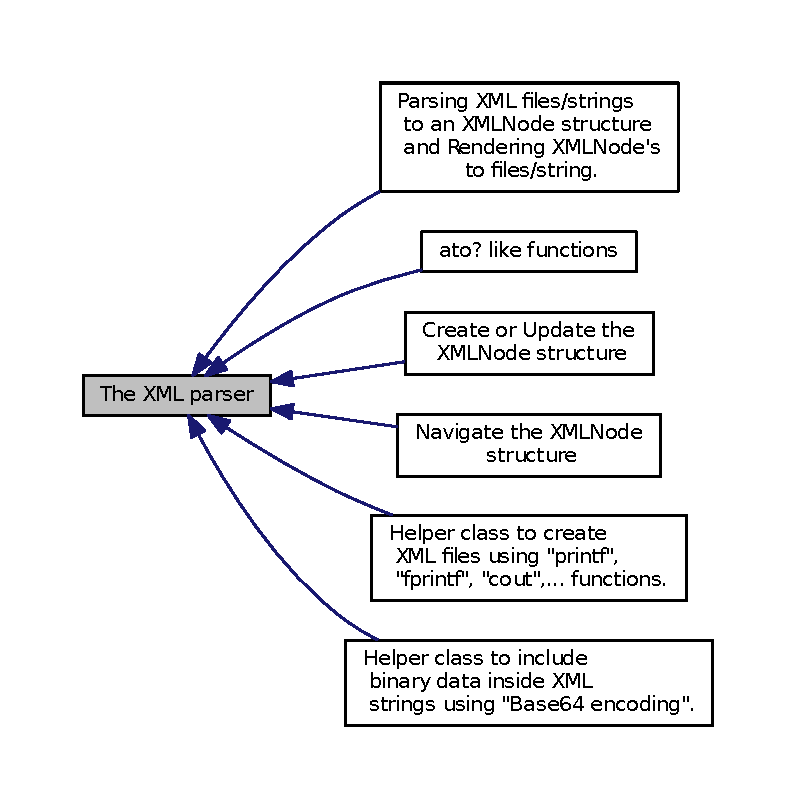
\includegraphics[width=350pt]{group__XMLParserGeneral}
\end{center}
\end{figure}
\subsection*{Modules}
\begin{DoxyCompactItemize}
\item 
\hyperlink{group__conversions}{Parsing X\-M\-L files/strings to an X\-M\-L\-Node structure and Rendering X\-M\-L\-Node's to files/string.}
\item 
\hyperlink{group__navigate}{Navigate the X\-M\-L\-Node structure}
\item 
\hyperlink{group__xmlModify}{Create or Update the X\-M\-L\-Node structure}
\item 
\hyperlink{group__atoX}{ato? like functions}
\item 
\hyperlink{group__ToXMLStringTool}{Helper class to create X\-M\-L files using \char`\"{}printf\char`\"{}, \char`\"{}fprintf\char`\"{}, \char`\"{}cout\char`\"{},... functions.}
\item 
\hyperlink{group__XMLParserBase64Tool}{Helper class to include binary data inside X\-M\-L strings using \char`\"{}\-Base64 encoding\char`\"{}.}
\end{DoxyCompactItemize}


\subsection{Detailed Description}

\hypertarget{group__conversions}{\section{Parsing X\-M\-L files/strings to an X\-M\-L\-Node structure and Rendering X\-M\-L\-Node's to files/string.}
\label{group__conversions}\index{Parsing X\-M\-L files/strings to an X\-M\-L\-Node structure and Rendering X\-M\-L\-Node's to files/string.@{Parsing X\-M\-L files/strings to an X\-M\-L\-Node structure and Rendering X\-M\-L\-Node's to files/string.}}
}
Collaboration diagram for Parsing X\-M\-L files/strings to an X\-M\-L\-Node structure and Rendering X\-M\-L\-Node's to files/string.\-:
\nopagebreak
\begin{figure}[H]
\begin{center}
\leavevmode
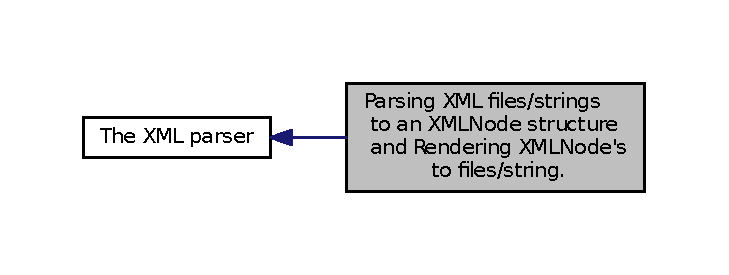
\includegraphics[width=350pt]{group__conversions}
\end{center}
\end{figure}
\subsection*{Functions}
\begin{DoxyCompactItemize}
\item 
static \hyperlink{structXMLNode}{X\-M\-L\-Node} \hyperlink{group__conversions_ga72125a4ccfae9b39bafab768346bbc7e}{X\-M\-L\-Node\-::parse\-String} (\hyperlink{xmlParser_8h_acdb0d6fd8dd596384b438d86cfb2b182}{X\-M\-L\-C\-S\-T\-R} lp\-X\-M\-L\-String, \hyperlink{xmlParser_8h_acdb0d6fd8dd596384b438d86cfb2b182}{X\-M\-L\-C\-S\-T\-R} tag=N\-U\-L\-L, \hyperlink{structXMLResults}{X\-M\-L\-Results} $\ast$p\-Results=N\-U\-L\-L)
\begin{DoxyCompactList}\small\item\em Parse an X\-M\-L string and return the root of a \hyperlink{structXMLNode}{X\-M\-L\-Node} tree representing the string. \end{DoxyCompactList}\item 
static \hyperlink{structXMLNode}{X\-M\-L\-Node} \hyperlink{group__conversions_gae984d7ebce97fad429b2b786439815fb}{X\-M\-L\-Node\-::parse\-File} (\hyperlink{xmlParser_8h_acdb0d6fd8dd596384b438d86cfb2b182}{X\-M\-L\-C\-S\-T\-R} filename, \hyperlink{xmlParser_8h_acdb0d6fd8dd596384b438d86cfb2b182}{X\-M\-L\-C\-S\-T\-R} tag=N\-U\-L\-L, \hyperlink{structXMLResults}{X\-M\-L\-Results} $\ast$p\-Results=N\-U\-L\-L)
\begin{DoxyCompactList}\small\item\em Parse an X\-M\-L file and return the root of a \hyperlink{structXMLNode}{X\-M\-L\-Node} tree representing the file. \end{DoxyCompactList}\item 
static \hyperlink{structXMLNode}{X\-M\-L\-Node} \hyperlink{group__conversions_ga46f99cf406604471e15d4378f74ecc63}{X\-M\-L\-Node\-::open\-File\-Helper} (\hyperlink{xmlParser_8h_acdb0d6fd8dd596384b438d86cfb2b182}{X\-M\-L\-C\-S\-T\-R} filename, \hyperlink{xmlParser_8h_acdb0d6fd8dd596384b438d86cfb2b182}{X\-M\-L\-C\-S\-T\-R} tag=N\-U\-L\-L)
\begin{DoxyCompactList}\small\item\em Parse an X\-M\-L file and return the root of a \hyperlink{structXMLNode}{X\-M\-L\-Node} tree representing the file. A very crude error checking is made. An attempt to guess the Char Encoding used in the file is made. \end{DoxyCompactList}\item 
static \hyperlink{xmlParser_8h_acdb0d6fd8dd596384b438d86cfb2b182}{X\-M\-L\-C\-S\-T\-R} \hyperlink{group__conversions_ga615a6ca792929132043d1de511023772}{X\-M\-L\-Node\-::get\-Error} (\hyperlink{xmlParser_8h_ac39bd07b1461aaa70afffe2d7162b4f5}{X\-M\-L\-Error} error)
\begin{DoxyCompactList}\small\item\em this gives you a user-\/friendly explanation of the parsing error \end{DoxyCompactList}\item 
\hyperlink{xmlParser_8h_a849d96105aa0c8f64b5c10d9151a3cdc}{X\-M\-L\-S\-T\-R} \hyperlink{group__conversions_gac8710ba5e7ff6e62a222445501ef9972}{X\-M\-L\-Node\-::create\-X\-M\-L\-String} (int n\-Format=1, int $\ast$pn\-Size=N\-U\-L\-L) const 
\begin{DoxyCompactList}\small\item\em Create an X\-M\-L string starting from the current \hyperlink{structXMLNode}{X\-M\-L\-Node}. \end{DoxyCompactList}\item 
\hyperlink{xmlParser_8h_ac39bd07b1461aaa70afffe2d7162b4f5}{X\-M\-L\-Error} \hyperlink{group__conversions_gab8d92d057c0072cc195b1935b2f53d80}{X\-M\-L\-Node\-::write\-To\-File} (\hyperlink{xmlParser_8h_acdb0d6fd8dd596384b438d86cfb2b182}{X\-M\-L\-C\-S\-T\-R} filename, const char $\ast$encoding=N\-U\-L\-L, char n\-Format=1) const 
\begin{DoxyCompactList}\small\item\em Save the content of an xml\-Node inside a file. \end{DoxyCompactList}\item 
static char \hyperlink{group__conversions_ga2e3943ac932bf3e786810234e7c295b9}{X\-M\-L\-Node\-::set\-Global\-Options} (X\-M\-L\-Char\-Encoding character\-Encoding=\hyperlink{structXMLNode_a81bcd09f9c752b65633c1ca28ea025f2a0b35b4d55aae2d232400578ab1123d5a}{X\-M\-L\-Node\-::char\-\_\-encoding\-\_\-\-U\-T\-F8}, char guess\-Wide\-Char\-Chars=1, char drop\-White\-Space=1, char remove\-Comments\-In\-Middle\-Of\-Text=1)
\begin{DoxyCompactList}\small\item\em Sets the global options for the conversions. \end{DoxyCompactList}\item 
static X\-M\-L\-Char\-Encoding \hyperlink{group__conversions_ga2fb8e9b250d669776e5e1962a70a4196}{X\-M\-L\-Node\-::guess\-Char\-Encoding} (void $\ast$buffer, int buf\-Len, char use\-X\-M\-L\-Encoding\-Attribute=1)
\begin{DoxyCompactList}\small\item\em Guess the character encoding of the string (ascii, utf8 or shift-\/\-J\-I\-S) \end{DoxyCompactList}\end{DoxyCompactItemize}


\subsection{Detailed Description}


\subsection{Function Documentation}
\hypertarget{group__conversions_gac8710ba5e7ff6e62a222445501ef9972}{\index{Parsing X\-M\-L files/strings to an X\-M\-L\-Node structure and Rendering X\-M\-L\-Node's to files/string.@{Parsing X\-M\-L files/strings to an X\-M\-L\-Node structure and Rendering X\-M\-L\-Node's to files/string.}!create\-X\-M\-L\-String@{create\-X\-M\-L\-String}}
\index{create\-X\-M\-L\-String@{create\-X\-M\-L\-String}!Parsing XML files/strings to an XMLNode structure and Rendering XMLNode's to files/string.@{Parsing X\-M\-L files/strings to an X\-M\-L\-Node structure and Rendering X\-M\-L\-Node's to files/string.}}
\subsubsection[{create\-X\-M\-L\-String}]{\setlength{\rightskip}{0pt plus 5cm}{\bf X\-M\-L\-S\-T\-R} X\-M\-L\-Node\-::create\-X\-M\-L\-String (
\begin{DoxyParamCaption}
\item[{int}]{n\-Format = {\ttfamily 1}, }
\item[{int $\ast$}]{pn\-Size = {\ttfamily NULL}}
\end{DoxyParamCaption}
) const}}\label{group__conversions_gac8710ba5e7ff6e62a222445501ef9972}


Create an X\-M\-L string starting from the current \hyperlink{structXMLNode}{X\-M\-L\-Node}. 

The returned string should be free'd using the \char`\"{}free\-X\-M\-L\-String\char`\"{} function. \begin{DoxyVerb}    If nFormat==0, no formatting is required otherwise this returns an user friendly XML string from a given element
    with appropriate white spaces and carriage returns. if pnSize is given it returns the size in character of the string.  \end{DoxyVerb}
 \hypertarget{group__conversions_ga615a6ca792929132043d1de511023772}{\index{Parsing X\-M\-L files/strings to an X\-M\-L\-Node structure and Rendering X\-M\-L\-Node's to files/string.@{Parsing X\-M\-L files/strings to an X\-M\-L\-Node structure and Rendering X\-M\-L\-Node's to files/string.}!get\-Error@{get\-Error}}
\index{get\-Error@{get\-Error}!Parsing XML files/strings to an XMLNode structure and Rendering XMLNode's to files/string.@{Parsing X\-M\-L files/strings to an X\-M\-L\-Node structure and Rendering X\-M\-L\-Node's to files/string.}}
\subsubsection[{get\-Error}]{\setlength{\rightskip}{0pt plus 5cm}static {\bf X\-M\-L\-C\-S\-T\-R} X\-M\-L\-Node\-::get\-Error (
\begin{DoxyParamCaption}
\item[{{\bf X\-M\-L\-Error}}]{error}
\end{DoxyParamCaption}
)\hspace{0.3cm}{\ttfamily [static]}}}\label{group__conversions_ga615a6ca792929132043d1de511023772}


this gives you a user-\/friendly explanation of the parsing error 

\hypertarget{group__conversions_ga2fb8e9b250d669776e5e1962a70a4196}{\index{Parsing X\-M\-L files/strings to an X\-M\-L\-Node structure and Rendering X\-M\-L\-Node's to files/string.@{Parsing X\-M\-L files/strings to an X\-M\-L\-Node structure and Rendering X\-M\-L\-Node's to files/string.}!guess\-Char\-Encoding@{guess\-Char\-Encoding}}
\index{guess\-Char\-Encoding@{guess\-Char\-Encoding}!Parsing XML files/strings to an XMLNode structure and Rendering XMLNode's to files/string.@{Parsing X\-M\-L files/strings to an X\-M\-L\-Node structure and Rendering X\-M\-L\-Node's to files/string.}}
\subsubsection[{guess\-Char\-Encoding}]{\setlength{\rightskip}{0pt plus 5cm}static X\-M\-L\-Char\-Encoding X\-M\-L\-Node\-::guess\-Char\-Encoding (
\begin{DoxyParamCaption}
\item[{void $\ast$}]{buffer, }
\item[{int}]{buf\-Len, }
\item[{char}]{use\-X\-M\-L\-Encoding\-Attribute = {\ttfamily 1}}
\end{DoxyParamCaption}
)\hspace{0.3cm}{\ttfamily [static]}}}\label{group__conversions_ga2fb8e9b250d669776e5e1962a70a4196}


Guess the character encoding of the string (ascii, utf8 or shift-\/\-J\-I\-S) 

The \char`\"{}guess\-Char\-Encoding\char`\"{} function try to guess the character encoding. You most-\/probably will never have to use this function. It then returns the appropriate value of the global parameter \char`\"{}character\-Encoding\char`\"{} described in the \hyperlink{group__conversions_ga2e3943ac932bf3e786810234e7c295b9}{X\-M\-L\-Node\-::set\-Global\-Options}. The guess is based on the content of a buffer of length \char`\"{}buf\-Len\char`\"{} bytes that contains the first bytes (minimum 25 bytes; 200 bytes is a good value) of the file to be parsed. The \hyperlink{group__conversions_ga46f99cf406604471e15d4378f74ecc63}{X\-M\-L\-Node\-::open\-File\-Helper} function is using this function to automatically compute the value of the \char`\"{}character\-Encoding\char`\"{} global parameter. There are several heuristics used to do the guess. One of the heuristic is based on the \char`\"{}encoding\char`\"{} attribute. The original X\-M\-L specifications forbids to use this attribute to do the guess but you can still use it if you set \char`\"{}use\-X\-M\-L\-Encoding\-Attribute\char`\"{} to 1 (this is the default behavior and the behavior of most parsers). If an inconsistency in the encoding is detected, then the return value is \char`\"{}0\char`\"{}. \hypertarget{group__conversions_ga46f99cf406604471e15d4378f74ecc63}{\index{Parsing X\-M\-L files/strings to an X\-M\-L\-Node structure and Rendering X\-M\-L\-Node's to files/string.@{Parsing X\-M\-L files/strings to an X\-M\-L\-Node structure and Rendering X\-M\-L\-Node's to files/string.}!open\-File\-Helper@{open\-File\-Helper}}
\index{open\-File\-Helper@{open\-File\-Helper}!Parsing XML files/strings to an XMLNode structure and Rendering XMLNode's to files/string.@{Parsing X\-M\-L files/strings to an X\-M\-L\-Node structure and Rendering X\-M\-L\-Node's to files/string.}}
\subsubsection[{open\-File\-Helper}]{\setlength{\rightskip}{0pt plus 5cm}static {\bf X\-M\-L\-Node} X\-M\-L\-Node\-::open\-File\-Helper (
\begin{DoxyParamCaption}
\item[{{\bf X\-M\-L\-C\-S\-T\-R}}]{filename, }
\item[{{\bf X\-M\-L\-C\-S\-T\-R}}]{tag = {\ttfamily NULL}}
\end{DoxyParamCaption}
)\hspace{0.3cm}{\ttfamily [static]}}}\label{group__conversions_ga46f99cf406604471e15d4378f74ecc63}


Parse an X\-M\-L file and return the root of a \hyperlink{structXMLNode}{X\-M\-L\-Node} tree representing the file. A very crude error checking is made. An attempt to guess the Char Encoding used in the file is made. 

The \char`\"{}open\-File\-Helper\char`\"{} function reports to the screen all the warnings and errors that occurred during parsing of the X\-M\-L file. This function also tries to guess char Encoding (U\-T\-F-\/8, A\-S\-C\-I\-I or S\-H\-I\-T-\/\-J\-I\-S) based on the first 200 bytes of the file. Since each application has its own way to report and deal with errors, you should rather use the \char`\"{}parse\-File\char`\"{} function to parse X\-M\-L files and program yourself thereafter an \char`\"{}error reporting\char`\"{} tailored for your needs (instead of using the very crude \char`\"{}error reporting\char`\"{} mechanism included inside the \char`\"{}open\-File\-Helper\char`\"{} function).

If the X\-M\-L document is corrupted, the \char`\"{}open\-File\-Helper\char`\"{} method will\-:
\begin{DoxyItemize}
\item display an error message on the console (or inside a message\-Box for windows).
\item stop execution (exit).
\end{DoxyItemize}

I strongly suggest that you write your own \char`\"{}open\-File\-Helper\char`\"{} method tailored to your needs. If you still want to parse the file, you can use the A\-P\-P\-R\-O\-X\-I\-M\-A\-T\-E\-\_\-\-P\-A\-R\-S\-I\-N\-G option as explained inside the note at the beginning of the \char`\"{}xml\-Parser.\-cpp\char`\"{} file.


\begin{DoxyParams}{Parameters}
{\em filename} & the path of the X\-M\-L file to parse. \\
\hline
{\em tag} & the name of the first tag inside the X\-M\-L file. If the tag parameter is omitted, this function returns a node that represents the head of the xml document including the declaration term ($<$? ... ?$>$). \\
\hline
\end{DoxyParams}
\hypertarget{group__conversions_gae984d7ebce97fad429b2b786439815fb}{\index{Parsing X\-M\-L files/strings to an X\-M\-L\-Node structure and Rendering X\-M\-L\-Node's to files/string.@{Parsing X\-M\-L files/strings to an X\-M\-L\-Node structure and Rendering X\-M\-L\-Node's to files/string.}!parse\-File@{parse\-File}}
\index{parse\-File@{parse\-File}!Parsing XML files/strings to an XMLNode structure and Rendering XMLNode's to files/string.@{Parsing X\-M\-L files/strings to an X\-M\-L\-Node structure and Rendering X\-M\-L\-Node's to files/string.}}
\subsubsection[{parse\-File}]{\setlength{\rightskip}{0pt plus 5cm}static {\bf X\-M\-L\-Node} X\-M\-L\-Node\-::parse\-File (
\begin{DoxyParamCaption}
\item[{{\bf X\-M\-L\-C\-S\-T\-R}}]{filename, }
\item[{{\bf X\-M\-L\-C\-S\-T\-R}}]{tag = {\ttfamily NULL}, }
\item[{{\bf X\-M\-L\-Results} $\ast$}]{p\-Results = {\ttfamily NULL}}
\end{DoxyParamCaption}
)\hspace{0.3cm}{\ttfamily [static]}}}\label{group__conversions_gae984d7ebce97fad429b2b786439815fb}


Parse an X\-M\-L file and return the root of a \hyperlink{structXMLNode}{X\-M\-L\-Node} tree representing the file. 

The \char`\"{}parse\-File\char`\"{} function parse an X\-M\-L file and return the root of a \hyperlink{structXMLNode}{X\-M\-L\-Node} tree. The \char`\"{}opposite\char`\"{} of this function is the function \char`\"{}write\-To\-File\char`\"{} that re-\/creates an X\-M\-L file from an \hyperlink{structXMLNode}{X\-M\-L\-Node} tree. If the X\-M\-L document is corrupted, the \char`\"{}parse\-File\char`\"{} method will initialize the \char`\"{}p\-Results\char`\"{} variable with some information that can be used to trace the error. If you still want to parse the file, you can use the A\-P\-P\-R\-O\-X\-I\-M\-A\-T\-E\-\_\-\-P\-A\-R\-S\-I\-N\-G option as explained inside the note at the beginning of the \char`\"{}xml\-Parser.\-cpp\char`\"{} file.


\begin{DoxyParams}{Parameters}
{\em filename} & the path to the X\-M\-L file to parse \\
\hline
{\em tag} & the name of the first tag inside the X\-M\-L file. If the tag parameter is omitted, this function returns a node that represents the head of the xml document including the declaration term ($<$? ... ?$>$). \\
\hline
{\em p\-Results} & a pointer to a \hyperlink{structXMLResults}{X\-M\-L\-Results} variable that will contain some information that can be used to trace the X\-M\-L parsing error. You can have a user-\/friendly explanation of the parsing error with the \char`\"{}get\-Error\char`\"{} function. \\
\hline
\end{DoxyParams}
\hypertarget{group__conversions_ga72125a4ccfae9b39bafab768346bbc7e}{\index{Parsing X\-M\-L files/strings to an X\-M\-L\-Node structure and Rendering X\-M\-L\-Node's to files/string.@{Parsing X\-M\-L files/strings to an X\-M\-L\-Node structure and Rendering X\-M\-L\-Node's to files/string.}!parse\-String@{parse\-String}}
\index{parse\-String@{parse\-String}!Parsing XML files/strings to an XMLNode structure and Rendering XMLNode's to files/string.@{Parsing X\-M\-L files/strings to an X\-M\-L\-Node structure and Rendering X\-M\-L\-Node's to files/string.}}
\subsubsection[{parse\-String}]{\setlength{\rightskip}{0pt plus 5cm}static {\bf X\-M\-L\-Node} X\-M\-L\-Node\-::parse\-String (
\begin{DoxyParamCaption}
\item[{{\bf X\-M\-L\-C\-S\-T\-R}}]{lp\-X\-M\-L\-String, }
\item[{{\bf X\-M\-L\-C\-S\-T\-R}}]{tag = {\ttfamily NULL}, }
\item[{{\bf X\-M\-L\-Results} $\ast$}]{p\-Results = {\ttfamily NULL}}
\end{DoxyParamCaption}
)\hspace{0.3cm}{\ttfamily [static]}}}\label{group__conversions_ga72125a4ccfae9b39bafab768346bbc7e}


Parse an X\-M\-L string and return the root of a \hyperlink{structXMLNode}{X\-M\-L\-Node} tree representing the string. 

The \char`\"{}parse\-String\char`\"{} function parse an X\-M\-L string and return the root of a \hyperlink{structXMLNode}{X\-M\-L\-Node} tree. The \char`\"{}opposite\char`\"{} of this function is the function \char`\"{}create\-X\-M\-L\-String\char`\"{} that re-\/creates an X\-M\-L string from an \hyperlink{structXMLNode}{X\-M\-L\-Node} tree. If the X\-M\-L document is corrupted, the \char`\"{}parse\-String\char`\"{} method will initialize the \char`\"{}p\-Results\char`\"{} variable with some information that can be used to trace the error. If you still want to parse the file, you can use the A\-P\-P\-R\-O\-X\-I\-M\-A\-T\-E\-\_\-\-P\-A\-R\-S\-I\-N\-G option as explained inside the note at the beginning of the \char`\"{}xml\-Parser.\-cpp\char`\"{} file.


\begin{DoxyParams}{Parameters}
{\em lp\-X\-M\-L\-String} & the X\-M\-L string to parse \\
\hline
{\em tag} & the name of the first tag inside the X\-M\-L file. If the tag parameter is omitted, this function returns a node that represents the head of the xml document including the declaration term ($<$? ... ?$>$). \\
\hline
{\em p\-Results} & a pointer to a \hyperlink{structXMLResults}{X\-M\-L\-Results} variable that will contain some information that can be used to trace the X\-M\-L parsing error. You can have a user-\/friendly explanation of the parsing error with the \char`\"{}get\-Error\char`\"{} function. \\
\hline
\end{DoxyParams}
\hypertarget{group__conversions_ga2e3943ac932bf3e786810234e7c295b9}{\index{Parsing X\-M\-L files/strings to an X\-M\-L\-Node structure and Rendering X\-M\-L\-Node's to files/string.@{Parsing X\-M\-L files/strings to an X\-M\-L\-Node structure and Rendering X\-M\-L\-Node's to files/string.}!set\-Global\-Options@{set\-Global\-Options}}
\index{set\-Global\-Options@{set\-Global\-Options}!Parsing XML files/strings to an XMLNode structure and Rendering XMLNode's to files/string.@{Parsing X\-M\-L files/strings to an X\-M\-L\-Node structure and Rendering X\-M\-L\-Node's to files/string.}}
\subsubsection[{set\-Global\-Options}]{\setlength{\rightskip}{0pt plus 5cm}static char X\-M\-L\-Node\-::set\-Global\-Options (
\begin{DoxyParamCaption}
\item[{{\bf X\-M\-L\-Char\-Encoding}}]{character\-Encoding = {\ttfamily {\bf X\-M\-L\-Node\-::char\-\_\-encoding\-\_\-\-U\-T\-F8}}, }
\item[{char}]{guess\-Wide\-Char\-Chars = {\ttfamily 1}, }
\item[{char}]{drop\-White\-Space = {\ttfamily 1}, }
\item[{char}]{remove\-Comments\-In\-Middle\-Of\-Text = {\ttfamily 1}}
\end{DoxyParamCaption}
)\hspace{0.3cm}{\ttfamily [static]}}}\label{group__conversions_ga2e3943ac932bf3e786810234e7c295b9}


Sets the global options for the conversions. 

The \char`\"{}set\-Global\-Options\char`\"{} function allows you to change four global parameters that affect string \& file parsing. First of all, you most-\/probably will never have to change these 3 global parameters.


\begin{DoxyParams}{Parameters}
{\em guess\-Wide\-Char\-Chars} & If \char`\"{}guess\-Wide\-Char\-Chars\char`\"{}=1 and if this library is compiled in Wide\-Char mode, then the \hyperlink{group__conversions_gae984d7ebce97fad429b2b786439815fb}{X\-M\-L\-Node\-::parse\-File} and \hyperlink{group__conversions_ga46f99cf406604471e15d4378f74ecc63}{X\-M\-L\-Node\-::open\-File\-Helper} functions will test if the file contains A\-S\-C\-I\-I characters. If this is the case, then the file will be loaded and converted in memory to Wide\-Char before being parsed. If 0, no conversion will be performed.\\
\hline
{\em guess\-Wide\-Char\-Chars} & If \char`\"{}guess\-Wide\-Char\-Chars\char`\"{}=1 and if this library is compiled in A\-S\-C\-I\-I/\-U\-T\-F8/char$\ast$ mode, then the \hyperlink{group__conversions_gae984d7ebce97fad429b2b786439815fb}{X\-M\-L\-Node\-::parse\-File} and \hyperlink{group__conversions_ga46f99cf406604471e15d4378f74ecc63}{X\-M\-L\-Node\-::open\-File\-Helper} functions will test if the file contains Wide\-Char characters. If this is the case, then the file will be loaded and converted in memory to A\-S\-C\-I\-I/\-U\-T\-F8/char$\ast$ before being parsed. If 0, no conversion will be performed.\\
\hline
{\em character\-Encoding} & This parameter is only meaningful when compiling in char$\ast$ mode (multibyte character mode). In wchar\-\_\-t$\ast$ (wide char mode), this parameter is ignored. This parameter should be one of the three currently recognized encodings\-: X\-M\-L\-Node\-::encoding\-\_\-\-U\-T\-F8, X\-M\-L\-Node\-::encoding\-\_\-ascii, X\-M\-L\-Node\-::encoding\-\_\-\-Shift\-J\-I\-S.\\
\hline
{\em drop\-White\-Space} & In most situations, text fields containing only white spaces (and carriage returns) are useless. Even more, these \char`\"{}empty\char`\"{} text fields are annoying because they increase the complexity of the user's code for parsing. So, 99\% of the time, it's better to drop the \char`\"{}empty\char`\"{} text fields. However The X\-M\-L specification indicates that no white spaces should be lost when parsing the file. So to be perfectly X\-M\-L-\/compliant, you should set drop\-White\-Space=0. A note of caution\-: if you set \char`\"{}drop\-White\-Space=0\char`\"{}, the parser will be slower and your code will be more complex.\\
\hline
{\em remove\-Comments\-In\-Middle\-Of\-Text} & To explain this parameter, let's consider this code\-: 
\begin{DoxyCode}
              \hyperlink{structXMLNode}{XMLNode} x=\hyperlink{group__conversions_ga72125a4ccfae9b39bafab768346bbc7e}{XMLNode::parseString}(\textcolor{stringliteral}{"
      <a>foo<!-- hello -->bar<!DOCTYPE world >chu</a>"},\textcolor{stringliteral}{"a"});
\end{DoxyCode}
 If remove\-Comments\-In\-Middle\-Of\-Text=0, then we will have\-: 
\begin{DoxyCode}
              x.\hyperlink{group__navigate_gaeb607292b18d4615b7c169c7c08c0a8b}{getText}(0) -> \textcolor{stringliteral}{"foo"}
              x.\hyperlink{group__navigate_gaeb607292b18d4615b7c169c7c08c0a8b}{getText}(1) -> \textcolor{stringliteral}{"bar"}
              x.\hyperlink{group__navigate_gaeb607292b18d4615b7c169c7c08c0a8b}{getText}(2) -> \textcolor{stringliteral}{"chu"}
              x.\hyperlink{group__navigate_gab99fbcb5534ab2194889c4802e290354}{getClear}(0) --> \textcolor{stringliteral}{"<!-- hello -->"}
              x.\hyperlink{group__navigate_gab99fbcb5534ab2194889c4802e290354}{getClear}(1) --> \textcolor{stringliteral}{"<!DOCTYPE world >"}
\end{DoxyCode}
 If remove\-Comments\-In\-Middle\-Of\-Text=1, then we will have\-: 
\begin{DoxyCode}
              x.\hyperlink{group__navigate_gaeb607292b18d4615b7c169c7c08c0a8b}{getText}(0) -> \textcolor{stringliteral}{"foobar"}
              x.\hyperlink{group__navigate_gaeb607292b18d4615b7c169c7c08c0a8b}{getText}(1) -> \textcolor{stringliteral}{"chu"}
              x.\hyperlink{group__navigate_gab99fbcb5534ab2194889c4802e290354}{getClear}(0) --> \textcolor{stringliteral}{"<!DOCTYPE world >"}
\end{DoxyCode}
\\
\hline
\end{DoxyParams}
\begin{DoxyReturn}{Returns}
\char`\"{}0\char`\"{} when there are no errors. If you try to set an unrecognized encoding then the return value will be \char`\"{}1\char`\"{} to signal an error.
\end{DoxyReturn}
\begin{DoxyNote}{Note}
Sometime, it's useful to set \char`\"{}guess\-Wide\-Char\-Chars=0\char`\"{} to disable any conversion because the test to detect the file-\/type (A\-S\-C\-I\-I/\-U\-T\-F8/char$\ast$ or Wide\-Char) may fail (rarely). 
\end{DoxyNote}
\hypertarget{group__conversions_gab8d92d057c0072cc195b1935b2f53d80}{\index{Parsing X\-M\-L files/strings to an X\-M\-L\-Node structure and Rendering X\-M\-L\-Node's to files/string.@{Parsing X\-M\-L files/strings to an X\-M\-L\-Node structure and Rendering X\-M\-L\-Node's to files/string.}!write\-To\-File@{write\-To\-File}}
\index{write\-To\-File@{write\-To\-File}!Parsing XML files/strings to an XMLNode structure and Rendering XMLNode's to files/string.@{Parsing X\-M\-L files/strings to an X\-M\-L\-Node structure and Rendering X\-M\-L\-Node's to files/string.}}
\subsubsection[{write\-To\-File}]{\setlength{\rightskip}{0pt plus 5cm}{\bf X\-M\-L\-Error} X\-M\-L\-Node\-::write\-To\-File (
\begin{DoxyParamCaption}
\item[{{\bf X\-M\-L\-C\-S\-T\-R}}]{filename, }
\item[{const char $\ast$}]{encoding = {\ttfamily NULL}, }
\item[{char}]{n\-Format = {\ttfamily 1}}
\end{DoxyParamCaption}
) const}}\label{group__conversions_gab8d92d057c0072cc195b1935b2f53d80}


Save the content of an xml\-Node inside a file. 

If n\-Format==0, no formatting is required otherwise this returns an user friendly X\-M\-L string from a given element with appropriate white spaces and carriage returns. If the global parameter \char`\"{}character\-Encoding==encoding\-\_\-\-U\-T\-F8\char`\"{}, then the \char`\"{}encoding\char`\"{} parameter is ignored and always set to \char`\"{}utf-\/8\char`\"{}. If the global parameter \char`\"{}character\-Encoding==encoding\-\_\-\-Shift\-J\-I\-S\char`\"{}, then the \char`\"{}encoding\char`\"{} parameter is ignored and always set to \char`\"{}\-S\-H\-I\-F\-T-\/\-J\-I\-S\char`\"{}. If \char`\"{}\-\_\-\-X\-M\-L\-W\-I\-D\-E\-C\-H\-A\-R=1\char`\"{}, then the \char`\"{}encoding\char`\"{} parameter is ignored and always set to \char`\"{}utf-\/16\char`\"{}. If no \char`\"{}encoding\char`\"{} parameter is given the \char`\"{}\-I\-S\-O-\/8859-\/1\char`\"{} encoding is used. 
\hypertarget{group__navigate}{\section{Navigate the X\-M\-L\-Node structure}
\label{group__navigate}\index{Navigate the X\-M\-L\-Node structure@{Navigate the X\-M\-L\-Node structure}}
}
Collaboration diagram for Navigate the X\-M\-L\-Node structure\-:
\nopagebreak
\begin{figure}[H]
\begin{center}
\leavevmode
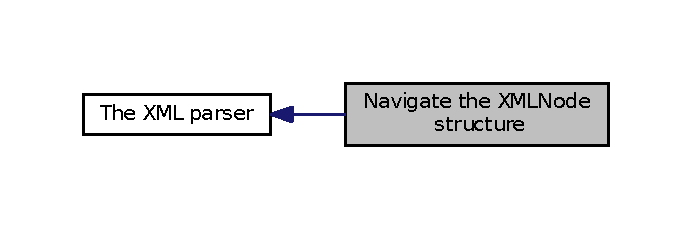
\includegraphics[width=332pt]{group__navigate}
\end{center}
\end{figure}
\subsection*{Functions}
\begin{DoxyCompactItemize}
\item 
\hyperlink{xmlParser_8h_acdb0d6fd8dd596384b438d86cfb2b182}{X\-M\-L\-C\-S\-T\-R} \hyperlink{group__navigate_ga7e07715aa0ed894da96bd66c90d423f0}{X\-M\-L\-Node\-::get\-Name} () const 
\begin{DoxyCompactList}\small\item\em name of the node \end{DoxyCompactList}\item 
\hyperlink{xmlParser_8h_acdb0d6fd8dd596384b438d86cfb2b182}{X\-M\-L\-C\-S\-T\-R} \hyperlink{group__navigate_gaeb607292b18d4615b7c169c7c08c0a8b}{X\-M\-L\-Node\-::get\-Text} (int i=0) const 
\begin{DoxyCompactList}\small\item\em return ith text field \end{DoxyCompactList}\item 
int \hyperlink{group__navigate_ga22e7e7cf8f173a1ec3ec3d6ff60819d9}{X\-M\-L\-Node\-::n\-Text} () const 
\begin{DoxyCompactList}\small\item\em nbr of text field \end{DoxyCompactList}\item 
\hyperlink{structXMLNode}{X\-M\-L\-Node} \hyperlink{group__navigate_gad30a8420556e220742c681e353a875d8}{X\-M\-L\-Node\-::get\-Parent\-Node} () const 
\begin{DoxyCompactList}\small\item\em return the parent node \end{DoxyCompactList}\item 
\hyperlink{structXMLNode}{X\-M\-L\-Node} \hyperlink{group__navigate_ga77a21438b6d48a52cf8a1270f82f4475}{X\-M\-L\-Node\-::get\-Child\-Node} (int i=0) const 
\begin{DoxyCompactList}\small\item\em return ith child node \end{DoxyCompactList}\item 
\hyperlink{structXMLNode}{X\-M\-L\-Node} \hyperlink{group__navigate_gaf46d002a855acb46c18e47b70e686808}{X\-M\-L\-Node\-::get\-Child\-Node} (\hyperlink{xmlParser_8h_acdb0d6fd8dd596384b438d86cfb2b182}{X\-M\-L\-C\-S\-T\-R} name, int i) const 
\begin{DoxyCompactList}\small\item\em return ith child node with specific name (return an empty node if failing). If i==-\/1, this returns the last \hyperlink{structXMLNode}{X\-M\-L\-Node} with the given name. \end{DoxyCompactList}\item 
\hyperlink{structXMLNode}{X\-M\-L\-Node} \hyperlink{group__navigate_gac2e8c96fc51b59b6667ee02785cb6943}{X\-M\-L\-Node\-::get\-Child\-Node} (\hyperlink{xmlParser_8h_acdb0d6fd8dd596384b438d86cfb2b182}{X\-M\-L\-C\-S\-T\-R} name, int $\ast$i=N\-U\-L\-L) const 
\begin{DoxyCompactList}\small\item\em return next child node with specific name (return an empty node if failing) \end{DoxyCompactList}\item 
\hyperlink{structXMLNode}{X\-M\-L\-Node} \hyperlink{group__navigate_ga5d2775ee0704a2c028d76d267db7960a}{X\-M\-L\-Node\-::get\-Child\-Node\-With\-Attribute} (\hyperlink{xmlParser_8h_acdb0d6fd8dd596384b438d86cfb2b182}{X\-M\-L\-C\-S\-T\-R} tag\-Name, \hyperlink{xmlParser_8h_acdb0d6fd8dd596384b438d86cfb2b182}{X\-M\-L\-C\-S\-T\-R} attribute\-Name, \hyperlink{xmlParser_8h_acdb0d6fd8dd596384b438d86cfb2b182}{X\-M\-L\-C\-S\-T\-R} attribute\-Value=N\-U\-L\-L, int $\ast$i=N\-U\-L\-L) const 
\begin{DoxyCompactList}\small\item\em return child node with specific name/attribute (return an empty node if failing) \end{DoxyCompactList}\item 
\hyperlink{structXMLNode}{X\-M\-L\-Node} \hyperlink{group__navigate_ga18176d2a9e4830dcb1bca62f9c664b15}{X\-M\-L\-Node\-::get\-Child\-Node\-By\-Path} (\hyperlink{xmlParser_8h_acdb0d6fd8dd596384b438d86cfb2b182}{X\-M\-L\-C\-S\-T\-R} path, char create\-Node\-If\-Missing=0, \hyperlink{xmlParser_8h_a9f587fbd233e721e8818a3bf8102838f}{X\-M\-L\-C\-H\-A\-R} sep='/')
\begin{DoxyCompactList}\small\item\em return the first child node with specific path \end{DoxyCompactList}\item 
\hyperlink{structXMLNode}{X\-M\-L\-Node} \hyperlink{group__navigate_ga0f3b175875c5d35a0dd88b4ed836079d}{X\-M\-L\-Node\-::get\-Child\-Node\-By\-Path\-Non\-Const} (\hyperlink{xmlParser_8h_a849d96105aa0c8f64b5c10d9151a3cdc}{X\-M\-L\-S\-T\-R} path, char create\-Node\-If\-Missing=0, \hyperlink{xmlParser_8h_a9f587fbd233e721e8818a3bf8102838f}{X\-M\-L\-C\-H\-A\-R} sep='/')
\begin{DoxyCompactList}\small\item\em return the first child node with specific path. \end{DoxyCompactList}\item 
int \hyperlink{group__navigate_ga8e52198f258167cd796dae21f1ffc352}{X\-M\-L\-Node\-::n\-Child\-Node} (\hyperlink{xmlParser_8h_acdb0d6fd8dd596384b438d86cfb2b182}{X\-M\-L\-C\-S\-T\-R} name) const 
\begin{DoxyCompactList}\small\item\em return the number of child node with specific name \end{DoxyCompactList}\item 
int \hyperlink{group__navigate_ga65aad0220b231b1bf5cd5c69d7c5de41}{X\-M\-L\-Node\-::n\-Child\-Node} () const 
\begin{DoxyCompactList}\small\item\em nbr of child node \end{DoxyCompactList}\item 
\hyperlink{structXMLAttribute}{X\-M\-L\-Attribute} \hyperlink{group__navigate_gaa07572a057ce7ffc8843e468d952f490}{X\-M\-L\-Node\-::get\-Attribute} (int i=0) const 
\begin{DoxyCompactList}\small\item\em return ith attribute \end{DoxyCompactList}\item 
\hyperlink{xmlParser_8h_acdb0d6fd8dd596384b438d86cfb2b182}{X\-M\-L\-C\-S\-T\-R} \hyperlink{group__navigate_ga67cf7717fa32175d8c6daa8f3f03ce7a}{X\-M\-L\-Node\-::get\-Attribute\-Name} (int i=0) const 
\begin{DoxyCompactList}\small\item\em return ith attribute name \end{DoxyCompactList}\item 
\hyperlink{xmlParser_8h_acdb0d6fd8dd596384b438d86cfb2b182}{X\-M\-L\-C\-S\-T\-R} \hyperlink{group__navigate_ga4abc0c5a3eec14e2f67518b625431541}{X\-M\-L\-Node\-::get\-Attribute\-Value} (int i=0) const 
\begin{DoxyCompactList}\small\item\em return ith attribute value \end{DoxyCompactList}\item 
char \hyperlink{group__navigate_ga8059888e8dd5d9caf04f765059c1b934}{X\-M\-L\-Node\-::is\-Attribute\-Set} (\hyperlink{xmlParser_8h_acdb0d6fd8dd596384b438d86cfb2b182}{X\-M\-L\-C\-S\-T\-R} name) const 
\begin{DoxyCompactList}\small\item\em test if an attribute with a specific name is given \end{DoxyCompactList}\item 
\hyperlink{xmlParser_8h_acdb0d6fd8dd596384b438d86cfb2b182}{X\-M\-L\-C\-S\-T\-R} \hyperlink{group__navigate_gaba897c342d3c55d71f4d987332789f69}{X\-M\-L\-Node\-::get\-Attribute} (\hyperlink{xmlParser_8h_acdb0d6fd8dd596384b438d86cfb2b182}{X\-M\-L\-C\-S\-T\-R} name, int i) const 
\begin{DoxyCompactList}\small\item\em return ith attribute content with specific name (return a N\-U\-L\-L if failing) \end{DoxyCompactList}\item 
\hyperlink{xmlParser_8h_acdb0d6fd8dd596384b438d86cfb2b182}{X\-M\-L\-C\-S\-T\-R} \hyperlink{group__navigate_ga23af0b5c771a9a5e7503a7dd2de72fc8}{X\-M\-L\-Node\-::get\-Attribute} (\hyperlink{xmlParser_8h_acdb0d6fd8dd596384b438d86cfb2b182}{X\-M\-L\-C\-S\-T\-R} name, int $\ast$i=N\-U\-L\-L) const 
\begin{DoxyCompactList}\small\item\em return next attribute content with specific name (return a N\-U\-L\-L if failing) \end{DoxyCompactList}\item 
int \hyperlink{group__navigate_ga9561f62b9ed1fa653fe9135c4f16a41d}{X\-M\-L\-Node\-::n\-Attribute} () const 
\begin{DoxyCompactList}\small\item\em nbr of attribute \end{DoxyCompactList}\item 
\hyperlink{structXMLClear}{X\-M\-L\-Clear} \hyperlink{group__navigate_gab99fbcb5534ab2194889c4802e290354}{X\-M\-L\-Node\-::get\-Clear} (int i=0) const 
\begin{DoxyCompactList}\small\item\em return ith clear field (comments) \end{DoxyCompactList}\item 
int \hyperlink{group__navigate_ga87d34f1ba1ba7d49e8aeacc63548dead}{X\-M\-L\-Node\-::n\-Clear} () const 
\begin{DoxyCompactList}\small\item\em nbr of clear field \end{DoxyCompactList}\item 
\hyperlink{structXMLNodeContents}{X\-M\-L\-Node\-Contents} \hyperlink{group__navigate_gaf56414ef38a13892afc4f22177a7760a}{X\-M\-L\-Node\-::enum\-Contents} (\hyperlink{xmlParser_8h_aab10d65aadeca1f026f6416becde7432}{X\-M\-L\-Element\-Position} i) const 
\begin{DoxyCompactList}\small\item\em enumerate all the different contents (attribute,child,text, clear) of the current \hyperlink{structXMLNode}{X\-M\-L\-Node}. The order is reflecting the order of the original file/string. N\-O\-T\-E\-: 0 $<$= i $<$ \hyperlink{group__navigate_ga8e9538deb9144dcab39b3a510a8202f1}{n\-Element()}; \end{DoxyCompactList}\item 
int \hyperlink{group__navigate_ga8e9538deb9144dcab39b3a510a8202f1}{X\-M\-L\-Node\-::n\-Element} () const 
\begin{DoxyCompactList}\small\item\em nbr of different contents for current node \end{DoxyCompactList}\item 
char \hyperlink{group__navigate_ga764ce0ff117af3e30ab0959114d36f9c}{X\-M\-L\-Node\-::is\-Empty} () const 
\begin{DoxyCompactList}\small\item\em is this node Empty? \end{DoxyCompactList}\item 
char \hyperlink{group__navigate_ga71df27d54a2dc09b0a456406a7e8c6d3}{X\-M\-L\-Node\-::is\-Declaration} () const 
\begin{DoxyCompactList}\small\item\em is this node a declaration $<$? .... ?$>$ \end{DoxyCompactList}\item 
\hyperlink{structXMLNode}{X\-M\-L\-Node} \hyperlink{group__navigate_gadb69f8d2db5997d84590ce3380e210f1}{X\-M\-L\-Node\-::deep\-Copy} () const 
\begin{DoxyCompactList}\small\item\em deep copy (duplicate/clone) a \hyperlink{structXMLNode}{X\-M\-L\-Node} \end{DoxyCompactList}\item 
static \hyperlink{structXMLNode}{X\-M\-L\-Node} \hyperlink{group__navigate_ga47c8238226a693d0aaf1111f1fa44ea0}{X\-M\-L\-Node\-::empty\-Node} ()
\begin{DoxyCompactList}\small\item\em return \hyperlink{structXMLNode_a90565bdb240d2f14f6a3d43f15100b63}{X\-M\-L\-Node\-::empty\-X\-M\-L\-Node}; \end{DoxyCompactList}\end{DoxyCompactItemize}


\subsection{Detailed Description}


\subsection{Function Documentation}
\hypertarget{group__navigate_gadb69f8d2db5997d84590ce3380e210f1}{\index{Navigate the X\-M\-L\-Node structure@{Navigate the X\-M\-L\-Node structure}!deep\-Copy@{deep\-Copy}}
\index{deep\-Copy@{deep\-Copy}!Navigate the XMLNode structure@{Navigate the X\-M\-L\-Node structure}}
\subsubsection[{deep\-Copy}]{\setlength{\rightskip}{0pt plus 5cm}{\bf X\-M\-L\-Node} X\-M\-L\-Node\-::deep\-Copy (
\begin{DoxyParamCaption}
{}
\end{DoxyParamCaption}
) const}}\label{group__navigate_gadb69f8d2db5997d84590ce3380e210f1}


deep copy (duplicate/clone) a \hyperlink{structXMLNode}{X\-M\-L\-Node} 

\hypertarget{group__navigate_ga47c8238226a693d0aaf1111f1fa44ea0}{\index{Navigate the X\-M\-L\-Node structure@{Navigate the X\-M\-L\-Node structure}!empty\-Node@{empty\-Node}}
\index{empty\-Node@{empty\-Node}!Navigate the XMLNode structure@{Navigate the X\-M\-L\-Node structure}}
\subsubsection[{empty\-Node}]{\setlength{\rightskip}{0pt plus 5cm}static {\bf X\-M\-L\-Node} X\-M\-L\-Node\-::empty\-Node (
\begin{DoxyParamCaption}
{}
\end{DoxyParamCaption}
)\hspace{0.3cm}{\ttfamily [static]}}}\label{group__navigate_ga47c8238226a693d0aaf1111f1fa44ea0}


return \hyperlink{structXMLNode_a90565bdb240d2f14f6a3d43f15100b63}{X\-M\-L\-Node\-::empty\-X\-M\-L\-Node}; 

\hypertarget{group__navigate_gaf56414ef38a13892afc4f22177a7760a}{\index{Navigate the X\-M\-L\-Node structure@{Navigate the X\-M\-L\-Node structure}!enum\-Contents@{enum\-Contents}}
\index{enum\-Contents@{enum\-Contents}!Navigate the XMLNode structure@{Navigate the X\-M\-L\-Node structure}}
\subsubsection[{enum\-Contents}]{\setlength{\rightskip}{0pt plus 5cm}{\bf X\-M\-L\-Node\-Contents} X\-M\-L\-Node\-::enum\-Contents (
\begin{DoxyParamCaption}
\item[{{\bf X\-M\-L\-Element\-Position}}]{i}
\end{DoxyParamCaption}
) const}}\label{group__navigate_gaf56414ef38a13892afc4f22177a7760a}


enumerate all the different contents (attribute,child,text, clear) of the current \hyperlink{structXMLNode}{X\-M\-L\-Node}. The order is reflecting the order of the original file/string. N\-O\-T\-E\-: 0 $<$= i $<$ \hyperlink{group__navigate_ga8e9538deb9144dcab39b3a510a8202f1}{n\-Element()}; 

\hypertarget{group__navigate_gaa07572a057ce7ffc8843e468d952f490}{\index{Navigate the X\-M\-L\-Node structure@{Navigate the X\-M\-L\-Node structure}!get\-Attribute@{get\-Attribute}}
\index{get\-Attribute@{get\-Attribute}!Navigate the XMLNode structure@{Navigate the X\-M\-L\-Node structure}}
\subsubsection[{get\-Attribute}]{\setlength{\rightskip}{0pt plus 5cm}{\bf X\-M\-L\-Attribute} X\-M\-L\-Node\-::get\-Attribute (
\begin{DoxyParamCaption}
\item[{int}]{i = {\ttfamily 0}}
\end{DoxyParamCaption}
) const}}\label{group__navigate_gaa07572a057ce7ffc8843e468d952f490}


return ith attribute 

\hypertarget{group__navigate_gaba897c342d3c55d71f4d987332789f69}{\index{Navigate the X\-M\-L\-Node structure@{Navigate the X\-M\-L\-Node structure}!get\-Attribute@{get\-Attribute}}
\index{get\-Attribute@{get\-Attribute}!Navigate the XMLNode structure@{Navigate the X\-M\-L\-Node structure}}
\subsubsection[{get\-Attribute}]{\setlength{\rightskip}{0pt plus 5cm}{\bf X\-M\-L\-C\-S\-T\-R} X\-M\-L\-Node\-::get\-Attribute (
\begin{DoxyParamCaption}
\item[{{\bf X\-M\-L\-C\-S\-T\-R}}]{name, }
\item[{int}]{i}
\end{DoxyParamCaption}
) const}}\label{group__navigate_gaba897c342d3c55d71f4d987332789f69}


return ith attribute content with specific name (return a N\-U\-L\-L if failing) 

\hypertarget{group__navigate_ga23af0b5c771a9a5e7503a7dd2de72fc8}{\index{Navigate the X\-M\-L\-Node structure@{Navigate the X\-M\-L\-Node structure}!get\-Attribute@{get\-Attribute}}
\index{get\-Attribute@{get\-Attribute}!Navigate the XMLNode structure@{Navigate the X\-M\-L\-Node structure}}
\subsubsection[{get\-Attribute}]{\setlength{\rightskip}{0pt plus 5cm}{\bf X\-M\-L\-C\-S\-T\-R} X\-M\-L\-Node\-::get\-Attribute (
\begin{DoxyParamCaption}
\item[{{\bf X\-M\-L\-C\-S\-T\-R}}]{name, }
\item[{int $\ast$}]{i = {\ttfamily NULL}}
\end{DoxyParamCaption}
) const}}\label{group__navigate_ga23af0b5c771a9a5e7503a7dd2de72fc8}


return next attribute content with specific name (return a N\-U\-L\-L if failing) 

\hypertarget{group__navigate_ga67cf7717fa32175d8c6daa8f3f03ce7a}{\index{Navigate the X\-M\-L\-Node structure@{Navigate the X\-M\-L\-Node structure}!get\-Attribute\-Name@{get\-Attribute\-Name}}
\index{get\-Attribute\-Name@{get\-Attribute\-Name}!Navigate the XMLNode structure@{Navigate the X\-M\-L\-Node structure}}
\subsubsection[{get\-Attribute\-Name}]{\setlength{\rightskip}{0pt plus 5cm}{\bf X\-M\-L\-C\-S\-T\-R} X\-M\-L\-Node\-::get\-Attribute\-Name (
\begin{DoxyParamCaption}
\item[{int}]{i = {\ttfamily 0}}
\end{DoxyParamCaption}
) const}}\label{group__navigate_ga67cf7717fa32175d8c6daa8f3f03ce7a}


return ith attribute name 

\hypertarget{group__navigate_ga4abc0c5a3eec14e2f67518b625431541}{\index{Navigate the X\-M\-L\-Node structure@{Navigate the X\-M\-L\-Node structure}!get\-Attribute\-Value@{get\-Attribute\-Value}}
\index{get\-Attribute\-Value@{get\-Attribute\-Value}!Navigate the XMLNode structure@{Navigate the X\-M\-L\-Node structure}}
\subsubsection[{get\-Attribute\-Value}]{\setlength{\rightskip}{0pt plus 5cm}{\bf X\-M\-L\-C\-S\-T\-R} X\-M\-L\-Node\-::get\-Attribute\-Value (
\begin{DoxyParamCaption}
\item[{int}]{i = {\ttfamily 0}}
\end{DoxyParamCaption}
) const}}\label{group__navigate_ga4abc0c5a3eec14e2f67518b625431541}


return ith attribute value 

\hypertarget{group__navigate_ga77a21438b6d48a52cf8a1270f82f4475}{\index{Navigate the X\-M\-L\-Node structure@{Navigate the X\-M\-L\-Node structure}!get\-Child\-Node@{get\-Child\-Node}}
\index{get\-Child\-Node@{get\-Child\-Node}!Navigate the XMLNode structure@{Navigate the X\-M\-L\-Node structure}}
\subsubsection[{get\-Child\-Node}]{\setlength{\rightskip}{0pt plus 5cm}{\bf X\-M\-L\-Node} X\-M\-L\-Node\-::get\-Child\-Node (
\begin{DoxyParamCaption}
\item[{int}]{i = {\ttfamily 0}}
\end{DoxyParamCaption}
) const}}\label{group__navigate_ga77a21438b6d48a52cf8a1270f82f4475}


return ith child node 

\hypertarget{group__navigate_gaf46d002a855acb46c18e47b70e686808}{\index{Navigate the X\-M\-L\-Node structure@{Navigate the X\-M\-L\-Node structure}!get\-Child\-Node@{get\-Child\-Node}}
\index{get\-Child\-Node@{get\-Child\-Node}!Navigate the XMLNode structure@{Navigate the X\-M\-L\-Node structure}}
\subsubsection[{get\-Child\-Node}]{\setlength{\rightskip}{0pt plus 5cm}{\bf X\-M\-L\-Node} X\-M\-L\-Node\-::get\-Child\-Node (
\begin{DoxyParamCaption}
\item[{{\bf X\-M\-L\-C\-S\-T\-R}}]{name, }
\item[{int}]{i}
\end{DoxyParamCaption}
) const}}\label{group__navigate_gaf46d002a855acb46c18e47b70e686808}


return ith child node with specific name (return an empty node if failing). If i==-\/1, this returns the last \hyperlink{structXMLNode}{X\-M\-L\-Node} with the given name. 

\hypertarget{group__navigate_gac2e8c96fc51b59b6667ee02785cb6943}{\index{Navigate the X\-M\-L\-Node structure@{Navigate the X\-M\-L\-Node structure}!get\-Child\-Node@{get\-Child\-Node}}
\index{get\-Child\-Node@{get\-Child\-Node}!Navigate the XMLNode structure@{Navigate the X\-M\-L\-Node structure}}
\subsubsection[{get\-Child\-Node}]{\setlength{\rightskip}{0pt plus 5cm}{\bf X\-M\-L\-Node} X\-M\-L\-Node\-::get\-Child\-Node (
\begin{DoxyParamCaption}
\item[{{\bf X\-M\-L\-C\-S\-T\-R}}]{name, }
\item[{int $\ast$}]{i = {\ttfamily NULL}}
\end{DoxyParamCaption}
) const}}\label{group__navigate_gac2e8c96fc51b59b6667ee02785cb6943}


return next child node with specific name (return an empty node if failing) 

\hypertarget{group__navigate_ga18176d2a9e4830dcb1bca62f9c664b15}{\index{Navigate the X\-M\-L\-Node structure@{Navigate the X\-M\-L\-Node structure}!get\-Child\-Node\-By\-Path@{get\-Child\-Node\-By\-Path}}
\index{get\-Child\-Node\-By\-Path@{get\-Child\-Node\-By\-Path}!Navigate the XMLNode structure@{Navigate the X\-M\-L\-Node structure}}
\subsubsection[{get\-Child\-Node\-By\-Path}]{\setlength{\rightskip}{0pt plus 5cm}{\bf X\-M\-L\-Node} X\-M\-L\-Node\-::get\-Child\-Node\-By\-Path (
\begin{DoxyParamCaption}
\item[{{\bf X\-M\-L\-C\-S\-T\-R}}]{path, }
\item[{char}]{create\-Node\-If\-Missing = {\ttfamily 0}, }
\item[{{\bf X\-M\-L\-C\-H\-A\-R}}]{sep = {\ttfamily '/'}}
\end{DoxyParamCaption}
)}}\label{group__navigate_ga18176d2a9e4830dcb1bca62f9c664b15}


return the first child node with specific path 

\hypertarget{group__navigate_ga0f3b175875c5d35a0dd88b4ed836079d}{\index{Navigate the X\-M\-L\-Node structure@{Navigate the X\-M\-L\-Node structure}!get\-Child\-Node\-By\-Path\-Non\-Const@{get\-Child\-Node\-By\-Path\-Non\-Const}}
\index{get\-Child\-Node\-By\-Path\-Non\-Const@{get\-Child\-Node\-By\-Path\-Non\-Const}!Navigate the XMLNode structure@{Navigate the X\-M\-L\-Node structure}}
\subsubsection[{get\-Child\-Node\-By\-Path\-Non\-Const}]{\setlength{\rightskip}{0pt plus 5cm}{\bf X\-M\-L\-Node} X\-M\-L\-Node\-::get\-Child\-Node\-By\-Path\-Non\-Const (
\begin{DoxyParamCaption}
\item[{{\bf X\-M\-L\-S\-T\-R}}]{path, }
\item[{char}]{create\-Node\-If\-Missing = {\ttfamily 0}, }
\item[{{\bf X\-M\-L\-C\-H\-A\-R}}]{sep = {\ttfamily '/'}}
\end{DoxyParamCaption}
)}}\label{group__navigate_ga0f3b175875c5d35a0dd88b4ed836079d}


return the first child node with specific path. 

\hypertarget{group__navigate_ga5d2775ee0704a2c028d76d267db7960a}{\index{Navigate the X\-M\-L\-Node structure@{Navigate the X\-M\-L\-Node structure}!get\-Child\-Node\-With\-Attribute@{get\-Child\-Node\-With\-Attribute}}
\index{get\-Child\-Node\-With\-Attribute@{get\-Child\-Node\-With\-Attribute}!Navigate the XMLNode structure@{Navigate the X\-M\-L\-Node structure}}
\subsubsection[{get\-Child\-Node\-With\-Attribute}]{\setlength{\rightskip}{0pt plus 5cm}{\bf X\-M\-L\-Node} X\-M\-L\-Node\-::get\-Child\-Node\-With\-Attribute (
\begin{DoxyParamCaption}
\item[{{\bf X\-M\-L\-C\-S\-T\-R}}]{tag\-Name, }
\item[{{\bf X\-M\-L\-C\-S\-T\-R}}]{attribute\-Name, }
\item[{{\bf X\-M\-L\-C\-S\-T\-R}}]{attribute\-Value = {\ttfamily NULL}, }
\item[{int $\ast$}]{i = {\ttfamily NULL}}
\end{DoxyParamCaption}
) const}}\label{group__navigate_ga5d2775ee0704a2c028d76d267db7960a}


return child node with specific name/attribute (return an empty node if failing) 

\hypertarget{group__navigate_gab99fbcb5534ab2194889c4802e290354}{\index{Navigate the X\-M\-L\-Node structure@{Navigate the X\-M\-L\-Node structure}!get\-Clear@{get\-Clear}}
\index{get\-Clear@{get\-Clear}!Navigate the XMLNode structure@{Navigate the X\-M\-L\-Node structure}}
\subsubsection[{get\-Clear}]{\setlength{\rightskip}{0pt plus 5cm}{\bf X\-M\-L\-Clear} X\-M\-L\-Node\-::get\-Clear (
\begin{DoxyParamCaption}
\item[{int}]{i = {\ttfamily 0}}
\end{DoxyParamCaption}
) const}}\label{group__navigate_gab99fbcb5534ab2194889c4802e290354}


return ith clear field (comments) 

\hypertarget{group__navigate_ga7e07715aa0ed894da96bd66c90d423f0}{\index{Navigate the X\-M\-L\-Node structure@{Navigate the X\-M\-L\-Node structure}!get\-Name@{get\-Name}}
\index{get\-Name@{get\-Name}!Navigate the XMLNode structure@{Navigate the X\-M\-L\-Node structure}}
\subsubsection[{get\-Name}]{\setlength{\rightskip}{0pt plus 5cm}{\bf X\-M\-L\-C\-S\-T\-R} X\-M\-L\-Node\-::get\-Name (
\begin{DoxyParamCaption}
{}
\end{DoxyParamCaption}
) const}}\label{group__navigate_ga7e07715aa0ed894da96bd66c90d423f0}


name of the node 

\hypertarget{group__navigate_gad30a8420556e220742c681e353a875d8}{\index{Navigate the X\-M\-L\-Node structure@{Navigate the X\-M\-L\-Node structure}!get\-Parent\-Node@{get\-Parent\-Node}}
\index{get\-Parent\-Node@{get\-Parent\-Node}!Navigate the XMLNode structure@{Navigate the X\-M\-L\-Node structure}}
\subsubsection[{get\-Parent\-Node}]{\setlength{\rightskip}{0pt plus 5cm}{\bf X\-M\-L\-Node} X\-M\-L\-Node\-::get\-Parent\-Node (
\begin{DoxyParamCaption}
{}
\end{DoxyParamCaption}
) const}}\label{group__navigate_gad30a8420556e220742c681e353a875d8}


return the parent node 

\hypertarget{group__navigate_gaeb607292b18d4615b7c169c7c08c0a8b}{\index{Navigate the X\-M\-L\-Node structure@{Navigate the X\-M\-L\-Node structure}!get\-Text@{get\-Text}}
\index{get\-Text@{get\-Text}!Navigate the XMLNode structure@{Navigate the X\-M\-L\-Node structure}}
\subsubsection[{get\-Text}]{\setlength{\rightskip}{0pt plus 5cm}{\bf X\-M\-L\-C\-S\-T\-R} X\-M\-L\-Node\-::get\-Text (
\begin{DoxyParamCaption}
\item[{int}]{i = {\ttfamily 0}}
\end{DoxyParamCaption}
) const}}\label{group__navigate_gaeb607292b18d4615b7c169c7c08c0a8b}


return ith text field 

\hypertarget{group__navigate_ga8059888e8dd5d9caf04f765059c1b934}{\index{Navigate the X\-M\-L\-Node structure@{Navigate the X\-M\-L\-Node structure}!is\-Attribute\-Set@{is\-Attribute\-Set}}
\index{is\-Attribute\-Set@{is\-Attribute\-Set}!Navigate the XMLNode structure@{Navigate the X\-M\-L\-Node structure}}
\subsubsection[{is\-Attribute\-Set}]{\setlength{\rightskip}{0pt plus 5cm}char X\-M\-L\-Node\-::is\-Attribute\-Set (
\begin{DoxyParamCaption}
\item[{{\bf X\-M\-L\-C\-S\-T\-R}}]{name}
\end{DoxyParamCaption}
) const}}\label{group__navigate_ga8059888e8dd5d9caf04f765059c1b934}


test if an attribute with a specific name is given 

\hypertarget{group__navigate_ga71df27d54a2dc09b0a456406a7e8c6d3}{\index{Navigate the X\-M\-L\-Node structure@{Navigate the X\-M\-L\-Node structure}!is\-Declaration@{is\-Declaration}}
\index{is\-Declaration@{is\-Declaration}!Navigate the XMLNode structure@{Navigate the X\-M\-L\-Node structure}}
\subsubsection[{is\-Declaration}]{\setlength{\rightskip}{0pt plus 5cm}char X\-M\-L\-Node\-::is\-Declaration (
\begin{DoxyParamCaption}
{}
\end{DoxyParamCaption}
) const}}\label{group__navigate_ga71df27d54a2dc09b0a456406a7e8c6d3}


is this node a declaration $<$? .... ?$>$ 

\hypertarget{group__navigate_ga764ce0ff117af3e30ab0959114d36f9c}{\index{Navigate the X\-M\-L\-Node structure@{Navigate the X\-M\-L\-Node structure}!is\-Empty@{is\-Empty}}
\index{is\-Empty@{is\-Empty}!Navigate the XMLNode structure@{Navigate the X\-M\-L\-Node structure}}
\subsubsection[{is\-Empty}]{\setlength{\rightskip}{0pt plus 5cm}char X\-M\-L\-Node\-::is\-Empty (
\begin{DoxyParamCaption}
{}
\end{DoxyParamCaption}
) const}}\label{group__navigate_ga764ce0ff117af3e30ab0959114d36f9c}


is this node Empty? 

\hypertarget{group__navigate_ga9561f62b9ed1fa653fe9135c4f16a41d}{\index{Navigate the X\-M\-L\-Node structure@{Navigate the X\-M\-L\-Node structure}!n\-Attribute@{n\-Attribute}}
\index{n\-Attribute@{n\-Attribute}!Navigate the XMLNode structure@{Navigate the X\-M\-L\-Node structure}}
\subsubsection[{n\-Attribute}]{\setlength{\rightskip}{0pt plus 5cm}int X\-M\-L\-Node\-::n\-Attribute (
\begin{DoxyParamCaption}
{}
\end{DoxyParamCaption}
) const}}\label{group__navigate_ga9561f62b9ed1fa653fe9135c4f16a41d}


nbr of attribute 

\hypertarget{group__navigate_ga8e52198f258167cd796dae21f1ffc352}{\index{Navigate the X\-M\-L\-Node structure@{Navigate the X\-M\-L\-Node structure}!n\-Child\-Node@{n\-Child\-Node}}
\index{n\-Child\-Node@{n\-Child\-Node}!Navigate the XMLNode structure@{Navigate the X\-M\-L\-Node structure}}
\subsubsection[{n\-Child\-Node}]{\setlength{\rightskip}{0pt plus 5cm}int X\-M\-L\-Node\-::n\-Child\-Node (
\begin{DoxyParamCaption}
\item[{{\bf X\-M\-L\-C\-S\-T\-R}}]{name}
\end{DoxyParamCaption}
) const}}\label{group__navigate_ga8e52198f258167cd796dae21f1ffc352}


return the number of child node with specific name 

\hypertarget{group__navigate_ga65aad0220b231b1bf5cd5c69d7c5de41}{\index{Navigate the X\-M\-L\-Node structure@{Navigate the X\-M\-L\-Node structure}!n\-Child\-Node@{n\-Child\-Node}}
\index{n\-Child\-Node@{n\-Child\-Node}!Navigate the XMLNode structure@{Navigate the X\-M\-L\-Node structure}}
\subsubsection[{n\-Child\-Node}]{\setlength{\rightskip}{0pt plus 5cm}int X\-M\-L\-Node\-::n\-Child\-Node (
\begin{DoxyParamCaption}
{}
\end{DoxyParamCaption}
) const}}\label{group__navigate_ga65aad0220b231b1bf5cd5c69d7c5de41}


nbr of child node 

\hypertarget{group__navigate_ga87d34f1ba1ba7d49e8aeacc63548dead}{\index{Navigate the X\-M\-L\-Node structure@{Navigate the X\-M\-L\-Node structure}!n\-Clear@{n\-Clear}}
\index{n\-Clear@{n\-Clear}!Navigate the XMLNode structure@{Navigate the X\-M\-L\-Node structure}}
\subsubsection[{n\-Clear}]{\setlength{\rightskip}{0pt plus 5cm}int X\-M\-L\-Node\-::n\-Clear (
\begin{DoxyParamCaption}
{}
\end{DoxyParamCaption}
) const}}\label{group__navigate_ga87d34f1ba1ba7d49e8aeacc63548dead}


nbr of clear field 

\hypertarget{group__navigate_ga8e9538deb9144dcab39b3a510a8202f1}{\index{Navigate the X\-M\-L\-Node structure@{Navigate the X\-M\-L\-Node structure}!n\-Element@{n\-Element}}
\index{n\-Element@{n\-Element}!Navigate the XMLNode structure@{Navigate the X\-M\-L\-Node structure}}
\subsubsection[{n\-Element}]{\setlength{\rightskip}{0pt plus 5cm}int X\-M\-L\-Node\-::n\-Element (
\begin{DoxyParamCaption}
{}
\end{DoxyParamCaption}
) const}}\label{group__navigate_ga8e9538deb9144dcab39b3a510a8202f1}


nbr of different contents for current node 

\hypertarget{group__navigate_ga22e7e7cf8f173a1ec3ec3d6ff60819d9}{\index{Navigate the X\-M\-L\-Node structure@{Navigate the X\-M\-L\-Node structure}!n\-Text@{n\-Text}}
\index{n\-Text@{n\-Text}!Navigate the XMLNode structure@{Navigate the X\-M\-L\-Node structure}}
\subsubsection[{n\-Text}]{\setlength{\rightskip}{0pt plus 5cm}int X\-M\-L\-Node\-::n\-Text (
\begin{DoxyParamCaption}
{}
\end{DoxyParamCaption}
) const}}\label{group__navigate_ga22e7e7cf8f173a1ec3ec3d6ff60819d9}


nbr of text field 


\hypertarget{group__xmlModify}{\section{Create or Update the X\-M\-L\-Node structure}
\label{group__xmlModify}\index{Create or Update the X\-M\-L\-Node structure@{Create or Update the X\-M\-L\-Node structure}}
}
Collaboration diagram for Create or Update the X\-M\-L\-Node structure\-:
\nopagebreak
\begin{figure}[H]
\begin{center}
\leavevmode
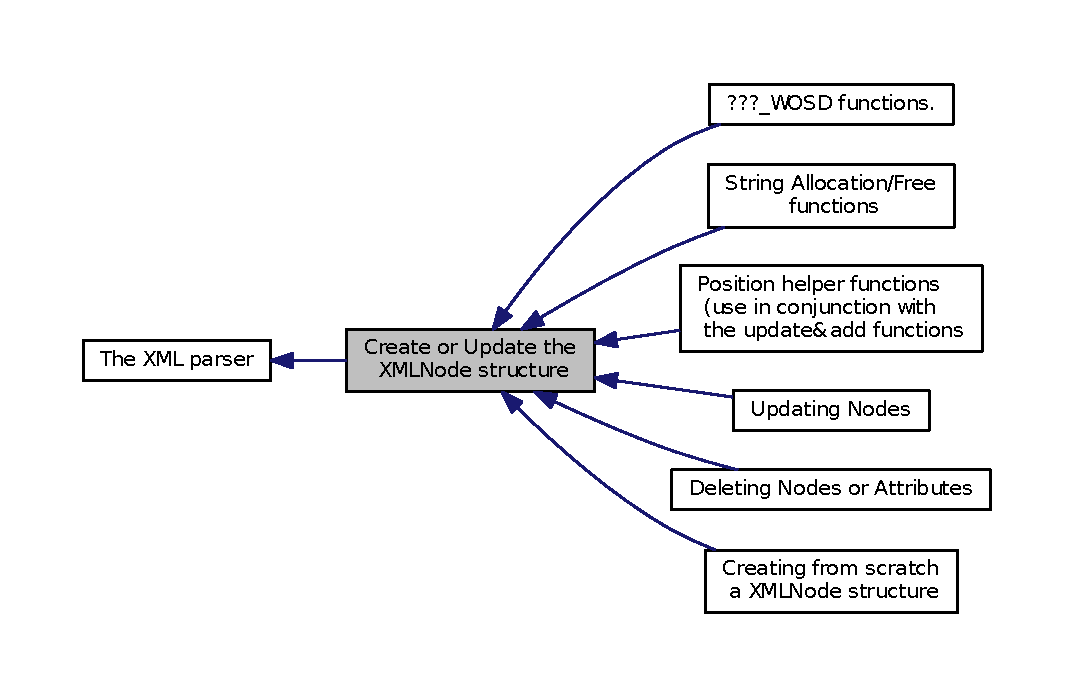
\includegraphics[width=350pt]{group__xmlModify}
\end{center}
\end{figure}
\subsection*{Modules}
\begin{DoxyCompactItemize}
\item 
\hyperlink{group__creation}{Creating from scratch a X\-M\-L\-Node structure}
\item 
\hyperlink{group__xmlUpdate}{Updating Nodes}
\item 
\hyperlink{group__xmlDelete}{Deleting Nodes or Attributes}
\item 
\hyperlink{group__xmlWOSD}{???\-\_\-\-W\-O\-S\-D functions.}
\item 
\hyperlink{group__xmlPosition}{Position helper functions (use in conjunction with the update\&add functions}
\item 
\hyperlink{group__StringAlloc}{String Allocation/\-Free functions}
\end{DoxyCompactItemize}


\subsection{Detailed Description}
The functions in this group allows you to create from scratch (or update) a \hyperlink{structXMLNode}{X\-M\-L\-Node} structure. Start by creating your top node with the \char`\"{}create\-X\-M\-L\-Top\-Node\char`\"{} function and then add new nodes with the \char`\"{}add\-Child\char`\"{} function. The parameter 'pos' gives the position where the child\-Node, the text or the X\-M\-L\-Clear\-Tag will be inserted. The default value (pos=-\/1) inserts at the end. The value (pos=0) insert at the beginning (Insertion at the beginning is slower than at the end). \par


R\-E\-M\-A\-R\-K\-: 0 $<$= pos $<$ n\-Child()+n\-Text()+n\-Clear() \par
 
\hypertarget{group__creation}{\section{Creating from scratch a X\-M\-L\-Node structure}
\label{group__creation}\index{Creating from scratch a X\-M\-L\-Node structure@{Creating from scratch a X\-M\-L\-Node structure}}
}
Collaboration diagram for Creating from scratch a X\-M\-L\-Node structure\-:
\nopagebreak
\begin{figure}[H]
\begin{center}
\leavevmode
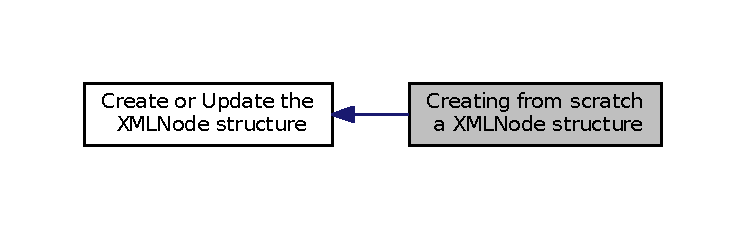
\includegraphics[width=350pt]{group__creation}
\end{center}
\end{figure}
\subsection*{Functions}
\begin{DoxyCompactItemize}
\item 
static \hyperlink{structXMLNode}{X\-M\-L\-Node} \hyperlink{group__creation_ga1e2d0403450db891eedc76b6bfdba452}{X\-M\-L\-Node\-::create\-X\-M\-L\-Top\-Node} (\hyperlink{xmlParser_8h_acdb0d6fd8dd596384b438d86cfb2b182}{X\-M\-L\-C\-S\-T\-R} lpsz\-Name, char is\-Declaration=\hyperlink{xmlParser_8h_aa93f0eb578d23995850d61f7d61c55c1}{F\-A\-L\-S\-E})
\begin{DoxyCompactList}\small\item\em Create the top node of an \hyperlink{structXMLNode}{X\-M\-L\-Node} structure. \end{DoxyCompactList}\item 
\hyperlink{structXMLNode}{X\-M\-L\-Node} \hyperlink{group__creation_ga51baa56a48f69cdea6f41ed38a2cbadd}{X\-M\-L\-Node\-::add\-Child} (\hyperlink{xmlParser_8h_acdb0d6fd8dd596384b438d86cfb2b182}{X\-M\-L\-C\-S\-T\-R} lpsz\-Name, char is\-Declaration=\hyperlink{xmlParser_8h_aa93f0eb578d23995850d61f7d61c55c1}{F\-A\-L\-S\-E}, \hyperlink{xmlParser_8h_aab10d65aadeca1f026f6416becde7432}{X\-M\-L\-Element\-Position} pos=-\/1)
\begin{DoxyCompactList}\small\item\em Add a new child node. \end{DoxyCompactList}\item 
\hyperlink{structXMLNode}{X\-M\-L\-Node} \hyperlink{group__creation_ga37c862f1d4a86f95417f97ceaa40d0fa}{X\-M\-L\-Node\-::add\-Child} (\hyperlink{structXMLNode}{X\-M\-L\-Node} node\-To\-Add, \hyperlink{xmlParser_8h_aab10d65aadeca1f026f6416becde7432}{X\-M\-L\-Element\-Position} pos=-\/1)
\begin{DoxyCompactList}\small\item\em If the \char`\"{}node\-To\-Add\char`\"{} has some parents, it will be detached from it's parents before being attached to the current \hyperlink{structXMLNode}{X\-M\-L\-Node}. \end{DoxyCompactList}\item 
\hyperlink{structXMLAttribute}{X\-M\-L\-Attribute} $\ast$ \hyperlink{group__creation_ga4f0e996a36cdda88b76bdf49d0d2e50c}{X\-M\-L\-Node\-::add\-Attribute} (\hyperlink{xmlParser_8h_acdb0d6fd8dd596384b438d86cfb2b182}{X\-M\-L\-C\-S\-T\-R} lpsz\-Name, \hyperlink{xmlParser_8h_acdb0d6fd8dd596384b438d86cfb2b182}{X\-M\-L\-C\-S\-T\-R} lpsz\-Valuev)
\begin{DoxyCompactList}\small\item\em Add a new attribute. \end{DoxyCompactList}\item 
\hyperlink{xmlParser_8h_acdb0d6fd8dd596384b438d86cfb2b182}{X\-M\-L\-C\-S\-T\-R} \hyperlink{group__creation_ga1de718e237befa215381d294fc644f11}{X\-M\-L\-Node\-::add\-Text} (\hyperlink{xmlParser_8h_acdb0d6fd8dd596384b438d86cfb2b182}{X\-M\-L\-C\-S\-T\-R} lpsz\-Value, \hyperlink{xmlParser_8h_aab10d65aadeca1f026f6416becde7432}{X\-M\-L\-Element\-Position} pos=-\/1)
\begin{DoxyCompactList}\small\item\em Add a new text content. \end{DoxyCompactList}\item 
\hyperlink{structXMLClear}{X\-M\-L\-Clear} $\ast$ \hyperlink{group__creation_gafb513cd0d881bcb153d702a885aebc44}{X\-M\-L\-Node\-::add\-Clear} (\hyperlink{xmlParser_8h_acdb0d6fd8dd596384b438d86cfb2b182}{X\-M\-L\-C\-S\-T\-R} lpsz\-Value, \hyperlink{xmlParser_8h_acdb0d6fd8dd596384b438d86cfb2b182}{X\-M\-L\-C\-S\-T\-R} lpsz\-Open=N\-U\-L\-L, \hyperlink{xmlParser_8h_acdb0d6fd8dd596384b438d86cfb2b182}{X\-M\-L\-C\-S\-T\-R} lpsz\-Close=N\-U\-L\-L, \hyperlink{xmlParser_8h_aab10d65aadeca1f026f6416becde7432}{X\-M\-L\-Element\-Position} pos=-\/1)
\end{DoxyCompactItemize}


\subsection{Detailed Description}


\subsection{Function Documentation}
\hypertarget{group__creation_ga4f0e996a36cdda88b76bdf49d0d2e50c}{\index{Creating from scratch a X\-M\-L\-Node structure@{Creating from scratch a X\-M\-L\-Node structure}!add\-Attribute@{add\-Attribute}}
\index{add\-Attribute@{add\-Attribute}!Creating from scratch a XMLNode structure@{Creating from scratch a X\-M\-L\-Node structure}}
\subsubsection[{add\-Attribute}]{\setlength{\rightskip}{0pt plus 5cm}{\bf X\-M\-L\-Attribute}$\ast$ X\-M\-L\-Node\-::add\-Attribute (
\begin{DoxyParamCaption}
\item[{{\bf X\-M\-L\-C\-S\-T\-R}}]{lpsz\-Name, }
\item[{{\bf X\-M\-L\-C\-S\-T\-R}}]{lpsz\-Valuev}
\end{DoxyParamCaption}
)}}\label{group__creation_ga4f0e996a36cdda88b76bdf49d0d2e50c}


Add a new attribute. 

\hypertarget{group__creation_ga51baa56a48f69cdea6f41ed38a2cbadd}{\index{Creating from scratch a X\-M\-L\-Node structure@{Creating from scratch a X\-M\-L\-Node structure}!add\-Child@{add\-Child}}
\index{add\-Child@{add\-Child}!Creating from scratch a XMLNode structure@{Creating from scratch a X\-M\-L\-Node structure}}
\subsubsection[{add\-Child}]{\setlength{\rightskip}{0pt plus 5cm}{\bf X\-M\-L\-Node} X\-M\-L\-Node\-::add\-Child (
\begin{DoxyParamCaption}
\item[{{\bf X\-M\-L\-C\-S\-T\-R}}]{lpsz\-Name, }
\item[{char}]{is\-Declaration = {\ttfamily {\bf F\-A\-L\-S\-E}}, }
\item[{{\bf X\-M\-L\-Element\-Position}}]{pos = {\ttfamily -\/1}}
\end{DoxyParamCaption}
)}}\label{group__creation_ga51baa56a48f69cdea6f41ed38a2cbadd}


Add a new child node. 

\hypertarget{group__creation_ga37c862f1d4a86f95417f97ceaa40d0fa}{\index{Creating from scratch a X\-M\-L\-Node structure@{Creating from scratch a X\-M\-L\-Node structure}!add\-Child@{add\-Child}}
\index{add\-Child@{add\-Child}!Creating from scratch a XMLNode structure@{Creating from scratch a X\-M\-L\-Node structure}}
\subsubsection[{add\-Child}]{\setlength{\rightskip}{0pt plus 5cm}{\bf X\-M\-L\-Node} X\-M\-L\-Node\-::add\-Child (
\begin{DoxyParamCaption}
\item[{{\bf X\-M\-L\-Node}}]{node\-To\-Add, }
\item[{{\bf X\-M\-L\-Element\-Position}}]{pos = {\ttfamily -\/1}}
\end{DoxyParamCaption}
)}}\label{group__creation_ga37c862f1d4a86f95417f97ceaa40d0fa}


If the \char`\"{}node\-To\-Add\char`\"{} has some parents, it will be detached from it's parents before being attached to the current \hyperlink{structXMLNode}{X\-M\-L\-Node}. 

\hypertarget{group__creation_gafb513cd0d881bcb153d702a885aebc44}{\index{Creating from scratch a X\-M\-L\-Node structure@{Creating from scratch a X\-M\-L\-Node structure}!add\-Clear@{add\-Clear}}
\index{add\-Clear@{add\-Clear}!Creating from scratch a XMLNode structure@{Creating from scratch a X\-M\-L\-Node structure}}
\subsubsection[{add\-Clear}]{\setlength{\rightskip}{0pt plus 5cm}{\bf X\-M\-L\-Clear}$\ast$ X\-M\-L\-Node\-::add\-Clear (
\begin{DoxyParamCaption}
\item[{{\bf X\-M\-L\-C\-S\-T\-R}}]{lpsz\-Value, }
\item[{{\bf X\-M\-L\-C\-S\-T\-R}}]{lpsz\-Open = {\ttfamily NULL}, }
\item[{{\bf X\-M\-L\-C\-S\-T\-R}}]{lpsz\-Close = {\ttfamily NULL}, }
\item[{{\bf X\-M\-L\-Element\-Position}}]{pos = {\ttfamily -\/1}}
\end{DoxyParamCaption}
)}}\label{group__creation_gafb513cd0d881bcb153d702a885aebc44}
Add a new clear tag 
\begin{DoxyParams}{Parameters}
{\em lpsz\-Open} & default value \char`\"{}$<$!\mbox{[}\-C\-D\-A\-T\-A\mbox{[}\char`\"{} \\
\hline
{\em lpsz\-Close} & default value \char`\"{}\mbox{]}\mbox{]}$>$\char`\"{} \\
\hline
{\em lpsz\-Value} & \\
\hline
{\em pos} & \\
\hline
\end{DoxyParams}
\hypertarget{group__creation_ga1de718e237befa215381d294fc644f11}{\index{Creating from scratch a X\-M\-L\-Node structure@{Creating from scratch a X\-M\-L\-Node structure}!add\-Text@{add\-Text}}
\index{add\-Text@{add\-Text}!Creating from scratch a XMLNode structure@{Creating from scratch a X\-M\-L\-Node structure}}
\subsubsection[{add\-Text}]{\setlength{\rightskip}{0pt plus 5cm}{\bf X\-M\-L\-C\-S\-T\-R} X\-M\-L\-Node\-::add\-Text (
\begin{DoxyParamCaption}
\item[{{\bf X\-M\-L\-C\-S\-T\-R}}]{lpsz\-Value, }
\item[{{\bf X\-M\-L\-Element\-Position}}]{pos = {\ttfamily -\/1}}
\end{DoxyParamCaption}
)}}\label{group__creation_ga1de718e237befa215381d294fc644f11}


Add a new text content. 

\hypertarget{group__creation_ga1e2d0403450db891eedc76b6bfdba452}{\index{Creating from scratch a X\-M\-L\-Node structure@{Creating from scratch a X\-M\-L\-Node structure}!create\-X\-M\-L\-Top\-Node@{create\-X\-M\-L\-Top\-Node}}
\index{create\-X\-M\-L\-Top\-Node@{create\-X\-M\-L\-Top\-Node}!Creating from scratch a XMLNode structure@{Creating from scratch a X\-M\-L\-Node structure}}
\subsubsection[{create\-X\-M\-L\-Top\-Node}]{\setlength{\rightskip}{0pt plus 5cm}static {\bf X\-M\-L\-Node} X\-M\-L\-Node\-::create\-X\-M\-L\-Top\-Node (
\begin{DoxyParamCaption}
\item[{{\bf X\-M\-L\-C\-S\-T\-R}}]{lpsz\-Name, }
\item[{char}]{is\-Declaration = {\ttfamily {\bf F\-A\-L\-S\-E}}}
\end{DoxyParamCaption}
)\hspace{0.3cm}{\ttfamily [static]}}}\label{group__creation_ga1e2d0403450db891eedc76b6bfdba452}


Create the top node of an \hyperlink{structXMLNode}{X\-M\-L\-Node} structure. 


\hypertarget{group__xmlUpdate}{\section{Updating Nodes}
\label{group__xmlUpdate}\index{Updating Nodes@{Updating Nodes}}
}
Collaboration diagram for Updating Nodes\-:
\nopagebreak
\begin{figure}[H]
\begin{center}
\leavevmode
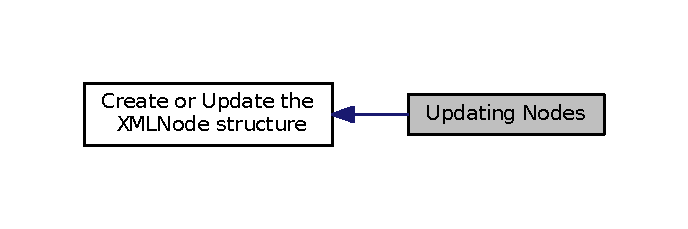
\includegraphics[width=330pt]{group__xmlUpdate}
\end{center}
\end{figure}
\subsection*{Functions}
\begin{DoxyCompactItemize}
\item 
\hyperlink{xmlParser_8h_acdb0d6fd8dd596384b438d86cfb2b182}{X\-M\-L\-C\-S\-T\-R} \hyperlink{group__xmlUpdate_gae08b643a2b87a77bad3c70eb57ea3043}{X\-M\-L\-Node\-::update\-Name} (\hyperlink{xmlParser_8h_acdb0d6fd8dd596384b438d86cfb2b182}{X\-M\-L\-C\-S\-T\-R} lpsz\-Name)
\begin{DoxyCompactList}\small\item\em change node's name \end{DoxyCompactList}\item 
\hyperlink{structXMLAttribute}{X\-M\-L\-Attribute} $\ast$ \hyperlink{group__xmlUpdate_ga49449139e44ef214d0c861e0b84f3757}{X\-M\-L\-Node\-::update\-Attribute} (\hyperlink{structXMLAttribute}{X\-M\-L\-Attribute} $\ast$new\-Attribute, \hyperlink{structXMLAttribute}{X\-M\-L\-Attribute} $\ast$old\-Attribute)
\begin{DoxyCompactList}\small\item\em if the attribute to update is missing, a new one will be added \end{DoxyCompactList}\item 
\hyperlink{structXMLAttribute}{X\-M\-L\-Attribute} $\ast$ \hyperlink{group__xmlUpdate_ga43e30a2630824996f5eb74ffcfa54adf}{X\-M\-L\-Node\-::update\-Attribute} (\hyperlink{xmlParser_8h_acdb0d6fd8dd596384b438d86cfb2b182}{X\-M\-L\-C\-S\-T\-R} lpsz\-New\-Value, \hyperlink{xmlParser_8h_acdb0d6fd8dd596384b438d86cfb2b182}{X\-M\-L\-C\-S\-T\-R} lpsz\-New\-Name=N\-U\-L\-L, int i=0)
\begin{DoxyCompactList}\small\item\em if the attribute to update is missing, a new one will be added \end{DoxyCompactList}\item 
\hyperlink{structXMLAttribute}{X\-M\-L\-Attribute} $\ast$ \hyperlink{group__xmlUpdate_gad334b0726cb7075a16aaca98aaff6372}{X\-M\-L\-Node\-::update\-Attribute} (\hyperlink{xmlParser_8h_acdb0d6fd8dd596384b438d86cfb2b182}{X\-M\-L\-C\-S\-T\-R} lpsz\-New\-Value, \hyperlink{xmlParser_8h_acdb0d6fd8dd596384b438d86cfb2b182}{X\-M\-L\-C\-S\-T\-R} lpsz\-New\-Name, \hyperlink{xmlParser_8h_acdb0d6fd8dd596384b438d86cfb2b182}{X\-M\-L\-C\-S\-T\-R} lpsz\-Old\-Name)
\begin{DoxyCompactList}\small\item\em set lpsz\-New\-Name=N\-U\-L\-L if you don't want to change the name of the attribute if the attribute to update is missing, a new one will be added \end{DoxyCompactList}\item 
\hyperlink{xmlParser_8h_acdb0d6fd8dd596384b438d86cfb2b182}{X\-M\-L\-C\-S\-T\-R} \hyperlink{group__xmlUpdate_gaad04ffd86ca67253bbc81f941608f8d2}{X\-M\-L\-Node\-::update\-Text} (\hyperlink{xmlParser_8h_acdb0d6fd8dd596384b438d86cfb2b182}{X\-M\-L\-C\-S\-T\-R} lpsz\-New\-Value, int i=0)
\begin{DoxyCompactList}\small\item\em if the text to update is missing, a new one will be added \end{DoxyCompactList}\item 
\hyperlink{xmlParser_8h_acdb0d6fd8dd596384b438d86cfb2b182}{X\-M\-L\-C\-S\-T\-R} \hyperlink{group__xmlUpdate_ga476a872fa595ea8416d2991ce3bea7a6}{X\-M\-L\-Node\-::update\-Text} (\hyperlink{xmlParser_8h_acdb0d6fd8dd596384b438d86cfb2b182}{X\-M\-L\-C\-S\-T\-R} lpsz\-New\-Value, \hyperlink{xmlParser_8h_acdb0d6fd8dd596384b438d86cfb2b182}{X\-M\-L\-C\-S\-T\-R} lpsz\-Old\-Value)
\begin{DoxyCompactList}\small\item\em if the text to update is missing, a new one will be added \end{DoxyCompactList}\item 
\hyperlink{structXMLClear}{X\-M\-L\-Clear} $\ast$ \hyperlink{group__xmlUpdate_gafe78ceff29e1853fdef9f9c3ac2605eb}{X\-M\-L\-Node\-::update\-Clear} (\hyperlink{xmlParser_8h_acdb0d6fd8dd596384b438d86cfb2b182}{X\-M\-L\-C\-S\-T\-R} lpsz\-New\-Content, int i=0)
\begin{DoxyCompactList}\small\item\em if the clear\-Tag to update is missing, a new one will be added \end{DoxyCompactList}\item 
\hyperlink{structXMLClear}{X\-M\-L\-Clear} $\ast$ \hyperlink{group__xmlUpdate_ga1279bfaade1376d25342440bd14dbb74}{X\-M\-L\-Node\-::update\-Clear} (\hyperlink{structXMLClear}{X\-M\-L\-Clear} $\ast$new\-P, \hyperlink{structXMLClear}{X\-M\-L\-Clear} $\ast$old\-P)
\begin{DoxyCompactList}\small\item\em if the clear\-Tag to update is missing, a new one will be added \end{DoxyCompactList}\item 
\hyperlink{structXMLClear}{X\-M\-L\-Clear} $\ast$ \hyperlink{group__xmlUpdate_ga49ad66755cd9b69fc1ec7a78cd162c70}{X\-M\-L\-Node\-::update\-Clear} (\hyperlink{xmlParser_8h_acdb0d6fd8dd596384b438d86cfb2b182}{X\-M\-L\-C\-S\-T\-R} lpsz\-New\-Value, \hyperlink{xmlParser_8h_acdb0d6fd8dd596384b438d86cfb2b182}{X\-M\-L\-C\-S\-T\-R} lpsz\-Old\-Value)
\begin{DoxyCompactList}\small\item\em if the clear\-Tag to update is missing, a new one will be added \end{DoxyCompactList}\end{DoxyCompactItemize}


\subsection{Detailed Description}
Some update functions\-: 

\subsection{Function Documentation}
\hypertarget{group__xmlUpdate_ga49449139e44ef214d0c861e0b84f3757}{\index{Updating Nodes@{Updating Nodes}!update\-Attribute@{update\-Attribute}}
\index{update\-Attribute@{update\-Attribute}!Updating Nodes@{Updating Nodes}}
\subsubsection[{update\-Attribute}]{\setlength{\rightskip}{0pt plus 5cm}{\bf X\-M\-L\-Attribute}$\ast$ X\-M\-L\-Node\-::update\-Attribute (
\begin{DoxyParamCaption}
\item[{{\bf X\-M\-L\-Attribute} $\ast$}]{new\-Attribute, }
\item[{{\bf X\-M\-L\-Attribute} $\ast$}]{old\-Attribute}
\end{DoxyParamCaption}
)}}\label{group__xmlUpdate_ga49449139e44ef214d0c861e0b84f3757}


if the attribute to update is missing, a new one will be added 

\hypertarget{group__xmlUpdate_ga43e30a2630824996f5eb74ffcfa54adf}{\index{Updating Nodes@{Updating Nodes}!update\-Attribute@{update\-Attribute}}
\index{update\-Attribute@{update\-Attribute}!Updating Nodes@{Updating Nodes}}
\subsubsection[{update\-Attribute}]{\setlength{\rightskip}{0pt plus 5cm}{\bf X\-M\-L\-Attribute}$\ast$ X\-M\-L\-Node\-::update\-Attribute (
\begin{DoxyParamCaption}
\item[{{\bf X\-M\-L\-C\-S\-T\-R}}]{lpsz\-New\-Value, }
\item[{{\bf X\-M\-L\-C\-S\-T\-R}}]{lpsz\-New\-Name = {\ttfamily NULL}, }
\item[{int}]{i = {\ttfamily 0}}
\end{DoxyParamCaption}
)}}\label{group__xmlUpdate_ga43e30a2630824996f5eb74ffcfa54adf}


if the attribute to update is missing, a new one will be added 

\hypertarget{group__xmlUpdate_gad334b0726cb7075a16aaca98aaff6372}{\index{Updating Nodes@{Updating Nodes}!update\-Attribute@{update\-Attribute}}
\index{update\-Attribute@{update\-Attribute}!Updating Nodes@{Updating Nodes}}
\subsubsection[{update\-Attribute}]{\setlength{\rightskip}{0pt plus 5cm}{\bf X\-M\-L\-Attribute}$\ast$ X\-M\-L\-Node\-::update\-Attribute (
\begin{DoxyParamCaption}
\item[{{\bf X\-M\-L\-C\-S\-T\-R}}]{lpsz\-New\-Value, }
\item[{{\bf X\-M\-L\-C\-S\-T\-R}}]{lpsz\-New\-Name, }
\item[{{\bf X\-M\-L\-C\-S\-T\-R}}]{lpsz\-Old\-Name}
\end{DoxyParamCaption}
)}}\label{group__xmlUpdate_gad334b0726cb7075a16aaca98aaff6372}


set lpsz\-New\-Name=N\-U\-L\-L if you don't want to change the name of the attribute if the attribute to update is missing, a new one will be added 

\hypertarget{group__xmlUpdate_gafe78ceff29e1853fdef9f9c3ac2605eb}{\index{Updating Nodes@{Updating Nodes}!update\-Clear@{update\-Clear}}
\index{update\-Clear@{update\-Clear}!Updating Nodes@{Updating Nodes}}
\subsubsection[{update\-Clear}]{\setlength{\rightskip}{0pt plus 5cm}{\bf X\-M\-L\-Clear}$\ast$ X\-M\-L\-Node\-::update\-Clear (
\begin{DoxyParamCaption}
\item[{{\bf X\-M\-L\-C\-S\-T\-R}}]{lpsz\-New\-Content, }
\item[{int}]{i = {\ttfamily 0}}
\end{DoxyParamCaption}
)}}\label{group__xmlUpdate_gafe78ceff29e1853fdef9f9c3ac2605eb}


if the clear\-Tag to update is missing, a new one will be added 

\hypertarget{group__xmlUpdate_ga1279bfaade1376d25342440bd14dbb74}{\index{Updating Nodes@{Updating Nodes}!update\-Clear@{update\-Clear}}
\index{update\-Clear@{update\-Clear}!Updating Nodes@{Updating Nodes}}
\subsubsection[{update\-Clear}]{\setlength{\rightskip}{0pt plus 5cm}{\bf X\-M\-L\-Clear}$\ast$ X\-M\-L\-Node\-::update\-Clear (
\begin{DoxyParamCaption}
\item[{{\bf X\-M\-L\-Clear} $\ast$}]{new\-P, }
\item[{{\bf X\-M\-L\-Clear} $\ast$}]{old\-P}
\end{DoxyParamCaption}
)}}\label{group__xmlUpdate_ga1279bfaade1376d25342440bd14dbb74}


if the clear\-Tag to update is missing, a new one will be added 

\hypertarget{group__xmlUpdate_ga49ad66755cd9b69fc1ec7a78cd162c70}{\index{Updating Nodes@{Updating Nodes}!update\-Clear@{update\-Clear}}
\index{update\-Clear@{update\-Clear}!Updating Nodes@{Updating Nodes}}
\subsubsection[{update\-Clear}]{\setlength{\rightskip}{0pt plus 5cm}{\bf X\-M\-L\-Clear}$\ast$ X\-M\-L\-Node\-::update\-Clear (
\begin{DoxyParamCaption}
\item[{{\bf X\-M\-L\-C\-S\-T\-R}}]{lpsz\-New\-Value, }
\item[{{\bf X\-M\-L\-C\-S\-T\-R}}]{lpsz\-Old\-Value}
\end{DoxyParamCaption}
)}}\label{group__xmlUpdate_ga49ad66755cd9b69fc1ec7a78cd162c70}


if the clear\-Tag to update is missing, a new one will be added 

\hypertarget{group__xmlUpdate_gae08b643a2b87a77bad3c70eb57ea3043}{\index{Updating Nodes@{Updating Nodes}!update\-Name@{update\-Name}}
\index{update\-Name@{update\-Name}!Updating Nodes@{Updating Nodes}}
\subsubsection[{update\-Name}]{\setlength{\rightskip}{0pt plus 5cm}{\bf X\-M\-L\-C\-S\-T\-R} X\-M\-L\-Node\-::update\-Name (
\begin{DoxyParamCaption}
\item[{{\bf X\-M\-L\-C\-S\-T\-R}}]{lpsz\-Name}
\end{DoxyParamCaption}
)}}\label{group__xmlUpdate_gae08b643a2b87a77bad3c70eb57ea3043}


change node's name 

\hypertarget{group__xmlUpdate_gaad04ffd86ca67253bbc81f941608f8d2}{\index{Updating Nodes@{Updating Nodes}!update\-Text@{update\-Text}}
\index{update\-Text@{update\-Text}!Updating Nodes@{Updating Nodes}}
\subsubsection[{update\-Text}]{\setlength{\rightskip}{0pt plus 5cm}{\bf X\-M\-L\-C\-S\-T\-R} X\-M\-L\-Node\-::update\-Text (
\begin{DoxyParamCaption}
\item[{{\bf X\-M\-L\-C\-S\-T\-R}}]{lpsz\-New\-Value, }
\item[{int}]{i = {\ttfamily 0}}
\end{DoxyParamCaption}
)}}\label{group__xmlUpdate_gaad04ffd86ca67253bbc81f941608f8d2}


if the text to update is missing, a new one will be added 

\hypertarget{group__xmlUpdate_ga476a872fa595ea8416d2991ce3bea7a6}{\index{Updating Nodes@{Updating Nodes}!update\-Text@{update\-Text}}
\index{update\-Text@{update\-Text}!Updating Nodes@{Updating Nodes}}
\subsubsection[{update\-Text}]{\setlength{\rightskip}{0pt plus 5cm}{\bf X\-M\-L\-C\-S\-T\-R} X\-M\-L\-Node\-::update\-Text (
\begin{DoxyParamCaption}
\item[{{\bf X\-M\-L\-C\-S\-T\-R}}]{lpsz\-New\-Value, }
\item[{{\bf X\-M\-L\-C\-S\-T\-R}}]{lpsz\-Old\-Value}
\end{DoxyParamCaption}
)}}\label{group__xmlUpdate_ga476a872fa595ea8416d2991ce3bea7a6}


if the text to update is missing, a new one will be added 


\hypertarget{group__xmlDelete}{\section{Deleting Nodes or Attributes}
\label{group__xmlDelete}\index{Deleting Nodes or Attributes@{Deleting Nodes or Attributes}}
}
Collaboration diagram for Deleting Nodes or Attributes\-:
\nopagebreak
\begin{figure}[H]
\begin{center}
\leavevmode
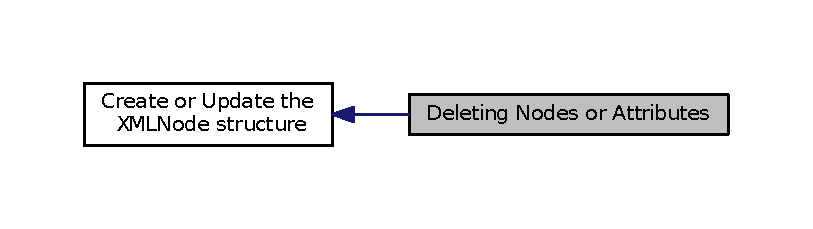
\includegraphics[width=350pt]{group__xmlDelete}
\end{center}
\end{figure}
\subsection*{Functions}
\begin{DoxyCompactItemize}
\item 
void \hyperlink{group__xmlDelete_gaa4d133999da220e916bdf3a969d493c4}{X\-M\-L\-Node\-::delete\-Node\-Content} ()
\begin{DoxyCompactList}\small\item\em The \char`\"{}delete\-Node\-Content\char`\"{} function forces the deletion of the content of this \hyperlink{structXMLNode}{X\-M\-L\-Node} and the subtree. \end{DoxyCompactList}\item 
void \hyperlink{group__xmlDelete_ga61b2405305063594b35b309cc2e22c01}{X\-M\-L\-Node\-::delete\-Attribute} (int i=0)
\begin{DoxyCompactList}\small\item\em Delete the ith attribute of the current \hyperlink{structXMLNode}{X\-M\-L\-Node}. \end{DoxyCompactList}\item 
void \hyperlink{group__xmlDelete_ga2b21339e5b370f1d7ebde2dc51217eed}{X\-M\-L\-Node\-::delete\-Attribute} (\hyperlink{xmlParser_8h_acdb0d6fd8dd596384b438d86cfb2b182}{X\-M\-L\-C\-S\-T\-R} lpsz\-Name)
\begin{DoxyCompactList}\small\item\em Delete the attribute with the given name (the \char`\"{}strcmp\char`\"{} function is used to find the right attribute) \end{DoxyCompactList}\item 
void \hyperlink{group__xmlDelete_ga6f00d7c1b4eaa29cfdd9d4a709495aca}{X\-M\-L\-Node\-::delete\-Attribute} (\hyperlink{structXMLAttribute}{X\-M\-L\-Attribute} $\ast$an\-Attribute)
\begin{DoxyCompactList}\small\item\em Delete the attribute with the name \char`\"{}an\-Attribute-\/$>$lpsz\-Name\char`\"{} (the \char`\"{}strcmp\char`\"{} function is used to find the right attribute) \end{DoxyCompactList}\item 
void \hyperlink{group__xmlDelete_ga14a49a23735ea10a44864cb6b4302250}{X\-M\-L\-Node\-::delete\-Text} (int i=0)
\begin{DoxyCompactList}\small\item\em Delete the Ith text content of the current \hyperlink{structXMLNode}{X\-M\-L\-Node}. \end{DoxyCompactList}\item 
void \hyperlink{group__xmlDelete_ga21ee499630d71ab6026753a85f02f582}{X\-M\-L\-Node\-::delete\-Text} (\hyperlink{xmlParser_8h_acdb0d6fd8dd596384b438d86cfb2b182}{X\-M\-L\-C\-S\-T\-R} lpsz\-Value)
\begin{DoxyCompactList}\small\item\em Delete the text content \char`\"{}lpsz\-Value\char`\"{} inside the current \hyperlink{structXMLNode}{X\-M\-L\-Node} (direct \char`\"{}pointer-\/to-\/pointer\char`\"{} comparison is used to find the right text) \end{DoxyCompactList}\item 
void \hyperlink{group__xmlDelete_ga44b72c82310eb4319dba46eb9cc9f6e9}{X\-M\-L\-Node\-::delete\-Clear} (int i=0)
\begin{DoxyCompactList}\small\item\em Delete the Ith clear tag inside the current \hyperlink{structXMLNode}{X\-M\-L\-Node}. \end{DoxyCompactList}\item 
void \hyperlink{group__xmlDelete_ga8fff4baa9a8000f8662ee302438fff64}{X\-M\-L\-Node\-::delete\-Clear} (\hyperlink{xmlParser_8h_acdb0d6fd8dd596384b438d86cfb2b182}{X\-M\-L\-C\-S\-T\-R} lpsz\-Value)
\begin{DoxyCompactList}\small\item\em Delete the clear tag \char`\"{}lpsz\-Value\char`\"{} inside the current \hyperlink{structXMLNode}{X\-M\-L\-Node} (direct \char`\"{}pointer-\/to-\/pointer\char`\"{} comparison is used to find the clear tag) \end{DoxyCompactList}\item 
void \hyperlink{group__xmlDelete_gae92182823d3d5b40893103ad222ec4a8}{X\-M\-L\-Node\-::delete\-Clear} (\hyperlink{structXMLClear}{X\-M\-L\-Clear} $\ast$p)
\begin{DoxyCompactList}\small\item\em Delete the clear tag \char`\"{}p\char`\"{} inside the current \hyperlink{structXMLNode}{X\-M\-L\-Node} (direct \char`\"{}pointer-\/to-\/pointer\char`\"{} comparison on the lpsz\-Name of the clear tag is used to find the clear tag) \end{DoxyCompactList}\end{DoxyCompactItemize}


\subsection{Detailed Description}
Some deletion functions\-: 

\subsection{Function Documentation}
\hypertarget{group__xmlDelete_ga61b2405305063594b35b309cc2e22c01}{\index{Deleting Nodes or Attributes@{Deleting Nodes or Attributes}!delete\-Attribute@{delete\-Attribute}}
\index{delete\-Attribute@{delete\-Attribute}!Deleting Nodes or Attributes@{Deleting Nodes or Attributes}}
\subsubsection[{delete\-Attribute}]{\setlength{\rightskip}{0pt plus 5cm}void X\-M\-L\-Node\-::delete\-Attribute (
\begin{DoxyParamCaption}
\item[{int}]{i = {\ttfamily 0}}
\end{DoxyParamCaption}
)}}\label{group__xmlDelete_ga61b2405305063594b35b309cc2e22c01}


Delete the ith attribute of the current \hyperlink{structXMLNode}{X\-M\-L\-Node}. 

\hypertarget{group__xmlDelete_ga2b21339e5b370f1d7ebde2dc51217eed}{\index{Deleting Nodes or Attributes@{Deleting Nodes or Attributes}!delete\-Attribute@{delete\-Attribute}}
\index{delete\-Attribute@{delete\-Attribute}!Deleting Nodes or Attributes@{Deleting Nodes or Attributes}}
\subsubsection[{delete\-Attribute}]{\setlength{\rightskip}{0pt plus 5cm}void X\-M\-L\-Node\-::delete\-Attribute (
\begin{DoxyParamCaption}
\item[{{\bf X\-M\-L\-C\-S\-T\-R}}]{lpsz\-Name}
\end{DoxyParamCaption}
)}}\label{group__xmlDelete_ga2b21339e5b370f1d7ebde2dc51217eed}


Delete the attribute with the given name (the \char`\"{}strcmp\char`\"{} function is used to find the right attribute) 

\hypertarget{group__xmlDelete_ga6f00d7c1b4eaa29cfdd9d4a709495aca}{\index{Deleting Nodes or Attributes@{Deleting Nodes or Attributes}!delete\-Attribute@{delete\-Attribute}}
\index{delete\-Attribute@{delete\-Attribute}!Deleting Nodes or Attributes@{Deleting Nodes or Attributes}}
\subsubsection[{delete\-Attribute}]{\setlength{\rightskip}{0pt plus 5cm}void X\-M\-L\-Node\-::delete\-Attribute (
\begin{DoxyParamCaption}
\item[{{\bf X\-M\-L\-Attribute} $\ast$}]{an\-Attribute}
\end{DoxyParamCaption}
)}}\label{group__xmlDelete_ga6f00d7c1b4eaa29cfdd9d4a709495aca}


Delete the attribute with the name \char`\"{}an\-Attribute-\/$>$lpsz\-Name\char`\"{} (the \char`\"{}strcmp\char`\"{} function is used to find the right attribute) 

\hypertarget{group__xmlDelete_ga44b72c82310eb4319dba46eb9cc9f6e9}{\index{Deleting Nodes or Attributes@{Deleting Nodes or Attributes}!delete\-Clear@{delete\-Clear}}
\index{delete\-Clear@{delete\-Clear}!Deleting Nodes or Attributes@{Deleting Nodes or Attributes}}
\subsubsection[{delete\-Clear}]{\setlength{\rightskip}{0pt plus 5cm}void X\-M\-L\-Node\-::delete\-Clear (
\begin{DoxyParamCaption}
\item[{int}]{i = {\ttfamily 0}}
\end{DoxyParamCaption}
)}}\label{group__xmlDelete_ga44b72c82310eb4319dba46eb9cc9f6e9}


Delete the Ith clear tag inside the current \hyperlink{structXMLNode}{X\-M\-L\-Node}. 

\hypertarget{group__xmlDelete_ga8fff4baa9a8000f8662ee302438fff64}{\index{Deleting Nodes or Attributes@{Deleting Nodes or Attributes}!delete\-Clear@{delete\-Clear}}
\index{delete\-Clear@{delete\-Clear}!Deleting Nodes or Attributes@{Deleting Nodes or Attributes}}
\subsubsection[{delete\-Clear}]{\setlength{\rightskip}{0pt plus 5cm}void X\-M\-L\-Node\-::delete\-Clear (
\begin{DoxyParamCaption}
\item[{{\bf X\-M\-L\-C\-S\-T\-R}}]{lpsz\-Value}
\end{DoxyParamCaption}
)}}\label{group__xmlDelete_ga8fff4baa9a8000f8662ee302438fff64}


Delete the clear tag \char`\"{}lpsz\-Value\char`\"{} inside the current \hyperlink{structXMLNode}{X\-M\-L\-Node} (direct \char`\"{}pointer-\/to-\/pointer\char`\"{} comparison is used to find the clear tag) 

\hypertarget{group__xmlDelete_gae92182823d3d5b40893103ad222ec4a8}{\index{Deleting Nodes or Attributes@{Deleting Nodes or Attributes}!delete\-Clear@{delete\-Clear}}
\index{delete\-Clear@{delete\-Clear}!Deleting Nodes or Attributes@{Deleting Nodes or Attributes}}
\subsubsection[{delete\-Clear}]{\setlength{\rightskip}{0pt plus 5cm}void X\-M\-L\-Node\-::delete\-Clear (
\begin{DoxyParamCaption}
\item[{{\bf X\-M\-L\-Clear} $\ast$}]{p}
\end{DoxyParamCaption}
)}}\label{group__xmlDelete_gae92182823d3d5b40893103ad222ec4a8}


Delete the clear tag \char`\"{}p\char`\"{} inside the current \hyperlink{structXMLNode}{X\-M\-L\-Node} (direct \char`\"{}pointer-\/to-\/pointer\char`\"{} comparison on the lpsz\-Name of the clear tag is used to find the clear tag) 

\hypertarget{group__xmlDelete_gaa4d133999da220e916bdf3a969d493c4}{\index{Deleting Nodes or Attributes@{Deleting Nodes or Attributes}!delete\-Node\-Content@{delete\-Node\-Content}}
\index{delete\-Node\-Content@{delete\-Node\-Content}!Deleting Nodes or Attributes@{Deleting Nodes or Attributes}}
\subsubsection[{delete\-Node\-Content}]{\setlength{\rightskip}{0pt plus 5cm}void X\-M\-L\-Node\-::delete\-Node\-Content (
\begin{DoxyParamCaption}
{}
\end{DoxyParamCaption}
)}}\label{group__xmlDelete_gaa4d133999da220e916bdf3a969d493c4}


The \char`\"{}delete\-Node\-Content\char`\"{} function forces the deletion of the content of this \hyperlink{structXMLNode}{X\-M\-L\-Node} and the subtree. 

\begin{DoxyNote}{Note}
The \hyperlink{structXMLNode}{X\-M\-L\-Node} instances that are referring to the part of the subtree that has been deleted C\-A\-N\-N\-O\-T be used anymore!!. Unexpected results will occur if you continue using them. 
\end{DoxyNote}
\hypertarget{group__xmlDelete_ga14a49a23735ea10a44864cb6b4302250}{\index{Deleting Nodes or Attributes@{Deleting Nodes or Attributes}!delete\-Text@{delete\-Text}}
\index{delete\-Text@{delete\-Text}!Deleting Nodes or Attributes@{Deleting Nodes or Attributes}}
\subsubsection[{delete\-Text}]{\setlength{\rightskip}{0pt plus 5cm}void X\-M\-L\-Node\-::delete\-Text (
\begin{DoxyParamCaption}
\item[{int}]{i = {\ttfamily 0}}
\end{DoxyParamCaption}
)}}\label{group__xmlDelete_ga14a49a23735ea10a44864cb6b4302250}


Delete the Ith text content of the current \hyperlink{structXMLNode}{X\-M\-L\-Node}. 

\hypertarget{group__xmlDelete_ga21ee499630d71ab6026753a85f02f582}{\index{Deleting Nodes or Attributes@{Deleting Nodes or Attributes}!delete\-Text@{delete\-Text}}
\index{delete\-Text@{delete\-Text}!Deleting Nodes or Attributes@{Deleting Nodes or Attributes}}
\subsubsection[{delete\-Text}]{\setlength{\rightskip}{0pt plus 5cm}void X\-M\-L\-Node\-::delete\-Text (
\begin{DoxyParamCaption}
\item[{{\bf X\-M\-L\-C\-S\-T\-R}}]{lpsz\-Value}
\end{DoxyParamCaption}
)}}\label{group__xmlDelete_ga21ee499630d71ab6026753a85f02f582}


Delete the text content \char`\"{}lpsz\-Value\char`\"{} inside the current \hyperlink{structXMLNode}{X\-M\-L\-Node} (direct \char`\"{}pointer-\/to-\/pointer\char`\"{} comparison is used to find the right text) 


\hypertarget{group__xmlWOSD}{\section{???\-\_\-\-W\-O\-S\-D functions.}
\label{group__xmlWOSD}\index{???\-\_\-\-W\-O\-S\-D functions.@{???\-\_\-\-W\-O\-S\-D functions.}}
}
Collaboration diagram for ???\-\_\-\-W\-O\-S\-D functions.\-:
\nopagebreak
\begin{figure}[H]
\begin{center}
\leavevmode
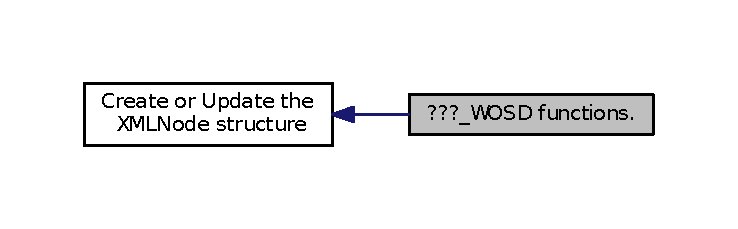
\includegraphics[width=350pt]{group__xmlWOSD}
\end{center}
\end{figure}
\subsection*{Functions}
\begin{DoxyCompactItemize}
\item 
static \hyperlink{structXMLNode}{X\-M\-L\-Node} \hyperlink{group__xmlWOSD_ga9c8b3bfa9671cb2a0a977ef30bab364a}{X\-M\-L\-Node\-::create\-X\-M\-L\-Top\-Node\-\_\-\-W\-O\-S\-D} (\hyperlink{xmlParser_8h_a849d96105aa0c8f64b5c10d9151a3cdc}{X\-M\-L\-S\-T\-R} lpsz\-Name, char is\-Declaration=\hyperlink{xmlParser_8h_aa93f0eb578d23995850d61f7d61c55c1}{F\-A\-L\-S\-E})
\begin{DoxyCompactList}\small\item\em Create the top node of an \hyperlink{structXMLNode}{X\-M\-L\-Node} structure. \end{DoxyCompactList}\item 
\hyperlink{structXMLNode}{X\-M\-L\-Node} \hyperlink{group__xmlWOSD_ga24b13602fdff0194b087df4eaf28e703}{X\-M\-L\-Node\-::add\-Child\-\_\-\-W\-O\-S\-D} (\hyperlink{xmlParser_8h_a849d96105aa0c8f64b5c10d9151a3cdc}{X\-M\-L\-S\-T\-R} lpsz\-Name, char is\-Declaration=\hyperlink{xmlParser_8h_aa93f0eb578d23995850d61f7d61c55c1}{F\-A\-L\-S\-E}, \hyperlink{xmlParser_8h_aab10d65aadeca1f026f6416becde7432}{X\-M\-L\-Element\-Position} pos=-\/1)
\begin{DoxyCompactList}\small\item\em Add a new child node. \end{DoxyCompactList}\item 
\hyperlink{structXMLAttribute}{X\-M\-L\-Attribute} $\ast$ \hyperlink{group__xmlWOSD_ga653039c9f5fb22076a00b258284c65ee}{X\-M\-L\-Node\-::add\-Attribute\-\_\-\-W\-O\-S\-D} (\hyperlink{xmlParser_8h_a849d96105aa0c8f64b5c10d9151a3cdc}{X\-M\-L\-S\-T\-R} lpsz\-Name, \hyperlink{xmlParser_8h_a849d96105aa0c8f64b5c10d9151a3cdc}{X\-M\-L\-S\-T\-R} lpsz\-Value)
\begin{DoxyCompactList}\small\item\em Add a new attribute. \end{DoxyCompactList}\item 
\hyperlink{xmlParser_8h_acdb0d6fd8dd596384b438d86cfb2b182}{X\-M\-L\-C\-S\-T\-R} \hyperlink{group__xmlWOSD_ga90944eacfeb994486e3ca83a68c35b6a}{X\-M\-L\-Node\-::add\-Text\-\_\-\-W\-O\-S\-D} (\hyperlink{xmlParser_8h_a849d96105aa0c8f64b5c10d9151a3cdc}{X\-M\-L\-S\-T\-R} lpsz\-Value, \hyperlink{xmlParser_8h_aab10d65aadeca1f026f6416becde7432}{X\-M\-L\-Element\-Position} pos=-\/1)
\begin{DoxyCompactList}\small\item\em Add a new text content. \end{DoxyCompactList}\item 
\hyperlink{structXMLClear}{X\-M\-L\-Clear} $\ast$ \hyperlink{group__xmlWOSD_ga6d3ed8368db156df576e0c54f5f45d30}{X\-M\-L\-Node\-::add\-Clear\-\_\-\-W\-O\-S\-D} (\hyperlink{xmlParser_8h_a849d96105aa0c8f64b5c10d9151a3cdc}{X\-M\-L\-S\-T\-R} lpsz\-Value, \hyperlink{xmlParser_8h_acdb0d6fd8dd596384b438d86cfb2b182}{X\-M\-L\-C\-S\-T\-R} lpsz\-Open=N\-U\-L\-L, \hyperlink{xmlParser_8h_acdb0d6fd8dd596384b438d86cfb2b182}{X\-M\-L\-C\-S\-T\-R} lpsz\-Close=N\-U\-L\-L, \hyperlink{xmlParser_8h_aab10d65aadeca1f026f6416becde7432}{X\-M\-L\-Element\-Position} pos=-\/1)
\begin{DoxyCompactList}\small\item\em Add a new clear Tag. \end{DoxyCompactList}\item 
\hyperlink{xmlParser_8h_acdb0d6fd8dd596384b438d86cfb2b182}{X\-M\-L\-C\-S\-T\-R} \hyperlink{group__xmlWOSD_ga5f35571651c6b629f5c8e5d02942a1c7}{X\-M\-L\-Node\-::update\-Name\-\_\-\-W\-O\-S\-D} (\hyperlink{xmlParser_8h_a849d96105aa0c8f64b5c10d9151a3cdc}{X\-M\-L\-S\-T\-R} lpsz\-Name)
\begin{DoxyCompactList}\small\item\em change node's name \end{DoxyCompactList}\item 
\hyperlink{structXMLAttribute}{X\-M\-L\-Attribute} $\ast$ \hyperlink{group__xmlWOSD_gaeb6533f46c1dd1843e33653612483a0c}{X\-M\-L\-Node\-::update\-Attribute\-\_\-\-W\-O\-S\-D} (\hyperlink{structXMLAttribute}{X\-M\-L\-Attribute} $\ast$new\-Attribute, \hyperlink{structXMLAttribute}{X\-M\-L\-Attribute} $\ast$old\-Attribute)
\begin{DoxyCompactList}\small\item\em if the attribute to update is missing, a new one will be added \end{DoxyCompactList}\item 
\hyperlink{structXMLAttribute}{X\-M\-L\-Attribute} $\ast$ \hyperlink{group__xmlWOSD_ga695e7ac29591363833575782243eff1b}{X\-M\-L\-Node\-::update\-Attribute\-\_\-\-W\-O\-S\-D} (\hyperlink{xmlParser_8h_a849d96105aa0c8f64b5c10d9151a3cdc}{X\-M\-L\-S\-T\-R} lpsz\-New\-Value, \hyperlink{xmlParser_8h_a849d96105aa0c8f64b5c10d9151a3cdc}{X\-M\-L\-S\-T\-R} lpsz\-New\-Name=N\-U\-L\-L, int i=0)
\begin{DoxyCompactList}\small\item\em if the attribute to update is missing, a new one will be added \end{DoxyCompactList}\item 
\hyperlink{structXMLAttribute}{X\-M\-L\-Attribute} $\ast$ \hyperlink{group__xmlWOSD_gababf6cef26796c45b88eb5772a9cafc4}{X\-M\-L\-Node\-::update\-Attribute\-\_\-\-W\-O\-S\-D} (\hyperlink{xmlParser_8h_a849d96105aa0c8f64b5c10d9151a3cdc}{X\-M\-L\-S\-T\-R} lpsz\-New\-Value, \hyperlink{xmlParser_8h_a849d96105aa0c8f64b5c10d9151a3cdc}{X\-M\-L\-S\-T\-R} lpsz\-New\-Name, \hyperlink{xmlParser_8h_acdb0d6fd8dd596384b438d86cfb2b182}{X\-M\-L\-C\-S\-T\-R} lpsz\-Old\-Name)
\begin{DoxyCompactList}\small\item\em set lpsz\-New\-Name=N\-U\-L\-L if you don't want to change the name of the attribute if the attribute to update is missing, a new one will be added \end{DoxyCompactList}\item 
\hyperlink{xmlParser_8h_acdb0d6fd8dd596384b438d86cfb2b182}{X\-M\-L\-C\-S\-T\-R} \hyperlink{group__xmlWOSD_ga8809eddad474e8bd7ad5f57aea7c77ac}{X\-M\-L\-Node\-::update\-Text\-\_\-\-W\-O\-S\-D} (\hyperlink{xmlParser_8h_a849d96105aa0c8f64b5c10d9151a3cdc}{X\-M\-L\-S\-T\-R} lpsz\-New\-Value, int i=0)
\begin{DoxyCompactList}\small\item\em if the text to update is missing, a new one will be added \end{DoxyCompactList}\item 
\hyperlink{xmlParser_8h_acdb0d6fd8dd596384b438d86cfb2b182}{X\-M\-L\-C\-S\-T\-R} \hyperlink{group__xmlWOSD_gae2c448a74bf74bcd502d4ba27c63eabc}{X\-M\-L\-Node\-::update\-Text\-\_\-\-W\-O\-S\-D} (\hyperlink{xmlParser_8h_a849d96105aa0c8f64b5c10d9151a3cdc}{X\-M\-L\-S\-T\-R} lpsz\-New\-Value, \hyperlink{xmlParser_8h_acdb0d6fd8dd596384b438d86cfb2b182}{X\-M\-L\-C\-S\-T\-R} lpsz\-Old\-Value)
\begin{DoxyCompactList}\small\item\em if the text to update is missing, a new one will be added \end{DoxyCompactList}\item 
\hyperlink{structXMLClear}{X\-M\-L\-Clear} $\ast$ \hyperlink{group__xmlWOSD_gac977a2e6b885ff4df3895deca771c363}{X\-M\-L\-Node\-::update\-Clear\-\_\-\-W\-O\-S\-D} (\hyperlink{xmlParser_8h_a849d96105aa0c8f64b5c10d9151a3cdc}{X\-M\-L\-S\-T\-R} lpsz\-New\-Content, int i=0)
\begin{DoxyCompactList}\small\item\em if the clear\-Tag to update is missing, a new one will be added \end{DoxyCompactList}\item 
\hyperlink{structXMLClear}{X\-M\-L\-Clear} $\ast$ \hyperlink{group__xmlWOSD_ga4863cd3e05ad9fac028321fffe8433b9}{X\-M\-L\-Node\-::update\-Clear\-\_\-\-W\-O\-S\-D} (\hyperlink{structXMLClear}{X\-M\-L\-Clear} $\ast$new\-P, \hyperlink{structXMLClear}{X\-M\-L\-Clear} $\ast$old\-P)
\begin{DoxyCompactList}\small\item\em if the clear\-Tag to update is missing, a new one will be added \end{DoxyCompactList}\item 
\hyperlink{structXMLClear}{X\-M\-L\-Clear} $\ast$ \hyperlink{group__xmlWOSD_gafd4fd40229c3c4ff67f019882f213cd4}{X\-M\-L\-Node\-::update\-Clear\-\_\-\-W\-O\-S\-D} (\hyperlink{xmlParser_8h_a849d96105aa0c8f64b5c10d9151a3cdc}{X\-M\-L\-S\-T\-R} lpsz\-New\-Value, \hyperlink{xmlParser_8h_acdb0d6fd8dd596384b438d86cfb2b182}{X\-M\-L\-C\-S\-T\-R} lpsz\-Old\-Value)
\begin{DoxyCompactList}\small\item\em if the clear\-Tag to update is missing, a new one will be added \end{DoxyCompactList}\end{DoxyCompactItemize}


\subsection{Detailed Description}
The strings given as parameters for the \char`\"{}add\char`\"{} and \char`\"{}update\char`\"{} methods that have a name with the postfix \char`\"{}\-\_\-\-W\-O\-S\-D\char`\"{} (that means \char`\"{}\-With\-Out String Duplication\char`\"{})(for example \char`\"{}add\-Text\-\_\-\-W\-O\-S\-D\char`\"{}) will be free'd by the \hyperlink{structXMLNode}{X\-M\-L\-Node} class. For example, it means that this is incorrect\-: 
\begin{DoxyCode}
           xNode.addText\_WOSD(\textcolor{stringliteral}{"foo"});
           xNode.updateAttribute\_WOSD(\textcolor{stringliteral}{"#newcolor"} ,NULL,\textcolor{stringliteral}{"color"});
\end{DoxyCode}
 In opposition, this is correct\-: 
\begin{DoxyCode}
           xNode.addText(\textcolor{stringliteral}{"foo"});
           xNode.addText\_WOSD(\hyperlink{group__StringAlloc_gac35b3be05a320f835b3976179637fe76}{stringDup}(\textcolor{stringliteral}{"foo"}));
           xNode.updateAttribute(\textcolor{stringliteral}{"#newcolor"} ,NULL,\textcolor{stringliteral}{"color"});
           xNode.updateAttribute\_WOSD(\hyperlink{group__StringAlloc_gac35b3be05a320f835b3976179637fe76}{stringDup}(\textcolor{stringliteral}{"#newcolor"}),NULL,\textcolor{stringliteral}{"
      color"});
\end{DoxyCode}
 Typically, you will never do\-: 
\begin{DoxyCode}
           \textcolor{keywordtype}{char} *b=(\textcolor{keywordtype}{char}*)malloc(...);
           xNode.addText(b);
           free(b);
\end{DoxyCode}
 ... but rather\-: 
\begin{DoxyCode}
           \textcolor{keywordtype}{char} *b=(\textcolor{keywordtype}{char}*)malloc(...);
           xNode.addText\_WOSD(b);
\end{DoxyCode}
 ('free(b)' is performed by the \hyperlink{structXMLNode}{X\-M\-L\-Node} class) 

\subsection{Function Documentation}
\hypertarget{group__xmlWOSD_ga653039c9f5fb22076a00b258284c65ee}{\index{???\-\_\-\-W\-O\-S\-D functions.@{???\-\_\-\-W\-O\-S\-D functions.}!add\-Attribute\-\_\-\-W\-O\-S\-D@{add\-Attribute\-\_\-\-W\-O\-S\-D}}
\index{add\-Attribute\-\_\-\-W\-O\-S\-D@{add\-Attribute\-\_\-\-W\-O\-S\-D}!???_WOSD functions.@{???\-\_\-\-W\-O\-S\-D functions.}}
\subsubsection[{add\-Attribute\-\_\-\-W\-O\-S\-D}]{\setlength{\rightskip}{0pt plus 5cm}{\bf X\-M\-L\-Attribute}$\ast$ X\-M\-L\-Node\-::add\-Attribute\-\_\-\-W\-O\-S\-D (
\begin{DoxyParamCaption}
\item[{{\bf X\-M\-L\-S\-T\-R}}]{lpsz\-Name, }
\item[{{\bf X\-M\-L\-S\-T\-R}}]{lpsz\-Value}
\end{DoxyParamCaption}
)}}\label{group__xmlWOSD_ga653039c9f5fb22076a00b258284c65ee}


Add a new attribute. 

\hypertarget{group__xmlWOSD_ga24b13602fdff0194b087df4eaf28e703}{\index{???\-\_\-\-W\-O\-S\-D functions.@{???\-\_\-\-W\-O\-S\-D functions.}!add\-Child\-\_\-\-W\-O\-S\-D@{add\-Child\-\_\-\-W\-O\-S\-D}}
\index{add\-Child\-\_\-\-W\-O\-S\-D@{add\-Child\-\_\-\-W\-O\-S\-D}!???_WOSD functions.@{???\-\_\-\-W\-O\-S\-D functions.}}
\subsubsection[{add\-Child\-\_\-\-W\-O\-S\-D}]{\setlength{\rightskip}{0pt plus 5cm}{\bf X\-M\-L\-Node} X\-M\-L\-Node\-::add\-Child\-\_\-\-W\-O\-S\-D (
\begin{DoxyParamCaption}
\item[{{\bf X\-M\-L\-S\-T\-R}}]{lpsz\-Name, }
\item[{char}]{is\-Declaration = {\ttfamily {\bf F\-A\-L\-S\-E}}, }
\item[{{\bf X\-M\-L\-Element\-Position}}]{pos = {\ttfamily -\/1}}
\end{DoxyParamCaption}
)}}\label{group__xmlWOSD_ga24b13602fdff0194b087df4eaf28e703}


Add a new child node. 

\hypertarget{group__xmlWOSD_ga6d3ed8368db156df576e0c54f5f45d30}{\index{???\-\_\-\-W\-O\-S\-D functions.@{???\-\_\-\-W\-O\-S\-D functions.}!add\-Clear\-\_\-\-W\-O\-S\-D@{add\-Clear\-\_\-\-W\-O\-S\-D}}
\index{add\-Clear\-\_\-\-W\-O\-S\-D@{add\-Clear\-\_\-\-W\-O\-S\-D}!???_WOSD functions.@{???\-\_\-\-W\-O\-S\-D functions.}}
\subsubsection[{add\-Clear\-\_\-\-W\-O\-S\-D}]{\setlength{\rightskip}{0pt plus 5cm}{\bf X\-M\-L\-Clear}$\ast$ X\-M\-L\-Node\-::add\-Clear\-\_\-\-W\-O\-S\-D (
\begin{DoxyParamCaption}
\item[{{\bf X\-M\-L\-S\-T\-R}}]{lpsz\-Value, }
\item[{{\bf X\-M\-L\-C\-S\-T\-R}}]{lpsz\-Open = {\ttfamily NULL}, }
\item[{{\bf X\-M\-L\-C\-S\-T\-R}}]{lpsz\-Close = {\ttfamily NULL}, }
\item[{{\bf X\-M\-L\-Element\-Position}}]{pos = {\ttfamily -\/1}}
\end{DoxyParamCaption}
)}}\label{group__xmlWOSD_ga6d3ed8368db156df576e0c54f5f45d30}


Add a new clear Tag. 

\hypertarget{group__xmlWOSD_ga90944eacfeb994486e3ca83a68c35b6a}{\index{???\-\_\-\-W\-O\-S\-D functions.@{???\-\_\-\-W\-O\-S\-D functions.}!add\-Text\-\_\-\-W\-O\-S\-D@{add\-Text\-\_\-\-W\-O\-S\-D}}
\index{add\-Text\-\_\-\-W\-O\-S\-D@{add\-Text\-\_\-\-W\-O\-S\-D}!???_WOSD functions.@{???\-\_\-\-W\-O\-S\-D functions.}}
\subsubsection[{add\-Text\-\_\-\-W\-O\-S\-D}]{\setlength{\rightskip}{0pt plus 5cm}{\bf X\-M\-L\-C\-S\-T\-R} X\-M\-L\-Node\-::add\-Text\-\_\-\-W\-O\-S\-D (
\begin{DoxyParamCaption}
\item[{{\bf X\-M\-L\-S\-T\-R}}]{lpsz\-Value, }
\item[{{\bf X\-M\-L\-Element\-Position}}]{pos = {\ttfamily -\/1}}
\end{DoxyParamCaption}
)}}\label{group__xmlWOSD_ga90944eacfeb994486e3ca83a68c35b6a}


Add a new text content. 

\hypertarget{group__xmlWOSD_ga9c8b3bfa9671cb2a0a977ef30bab364a}{\index{???\-\_\-\-W\-O\-S\-D functions.@{???\-\_\-\-W\-O\-S\-D functions.}!create\-X\-M\-L\-Top\-Node\-\_\-\-W\-O\-S\-D@{create\-X\-M\-L\-Top\-Node\-\_\-\-W\-O\-S\-D}}
\index{create\-X\-M\-L\-Top\-Node\-\_\-\-W\-O\-S\-D@{create\-X\-M\-L\-Top\-Node\-\_\-\-W\-O\-S\-D}!???_WOSD functions.@{???\-\_\-\-W\-O\-S\-D functions.}}
\subsubsection[{create\-X\-M\-L\-Top\-Node\-\_\-\-W\-O\-S\-D}]{\setlength{\rightskip}{0pt plus 5cm}static {\bf X\-M\-L\-Node} X\-M\-L\-Node\-::create\-X\-M\-L\-Top\-Node\-\_\-\-W\-O\-S\-D (
\begin{DoxyParamCaption}
\item[{{\bf X\-M\-L\-S\-T\-R}}]{lpsz\-Name, }
\item[{char}]{is\-Declaration = {\ttfamily {\bf F\-A\-L\-S\-E}}}
\end{DoxyParamCaption}
)\hspace{0.3cm}{\ttfamily [static]}}}\label{group__xmlWOSD_ga9c8b3bfa9671cb2a0a977ef30bab364a}


Create the top node of an \hyperlink{structXMLNode}{X\-M\-L\-Node} structure. 

\hypertarget{group__xmlWOSD_gaeb6533f46c1dd1843e33653612483a0c}{\index{???\-\_\-\-W\-O\-S\-D functions.@{???\-\_\-\-W\-O\-S\-D functions.}!update\-Attribute\-\_\-\-W\-O\-S\-D@{update\-Attribute\-\_\-\-W\-O\-S\-D}}
\index{update\-Attribute\-\_\-\-W\-O\-S\-D@{update\-Attribute\-\_\-\-W\-O\-S\-D}!???_WOSD functions.@{???\-\_\-\-W\-O\-S\-D functions.}}
\subsubsection[{update\-Attribute\-\_\-\-W\-O\-S\-D}]{\setlength{\rightskip}{0pt plus 5cm}{\bf X\-M\-L\-Attribute}$\ast$ X\-M\-L\-Node\-::update\-Attribute\-\_\-\-W\-O\-S\-D (
\begin{DoxyParamCaption}
\item[{{\bf X\-M\-L\-Attribute} $\ast$}]{new\-Attribute, }
\item[{{\bf X\-M\-L\-Attribute} $\ast$}]{old\-Attribute}
\end{DoxyParamCaption}
)}}\label{group__xmlWOSD_gaeb6533f46c1dd1843e33653612483a0c}


if the attribute to update is missing, a new one will be added 

\hypertarget{group__xmlWOSD_ga695e7ac29591363833575782243eff1b}{\index{???\-\_\-\-W\-O\-S\-D functions.@{???\-\_\-\-W\-O\-S\-D functions.}!update\-Attribute\-\_\-\-W\-O\-S\-D@{update\-Attribute\-\_\-\-W\-O\-S\-D}}
\index{update\-Attribute\-\_\-\-W\-O\-S\-D@{update\-Attribute\-\_\-\-W\-O\-S\-D}!???_WOSD functions.@{???\-\_\-\-W\-O\-S\-D functions.}}
\subsubsection[{update\-Attribute\-\_\-\-W\-O\-S\-D}]{\setlength{\rightskip}{0pt plus 5cm}{\bf X\-M\-L\-Attribute}$\ast$ X\-M\-L\-Node\-::update\-Attribute\-\_\-\-W\-O\-S\-D (
\begin{DoxyParamCaption}
\item[{{\bf X\-M\-L\-S\-T\-R}}]{lpsz\-New\-Value, }
\item[{{\bf X\-M\-L\-S\-T\-R}}]{lpsz\-New\-Name = {\ttfamily NULL}, }
\item[{int}]{i = {\ttfamily 0}}
\end{DoxyParamCaption}
)}}\label{group__xmlWOSD_ga695e7ac29591363833575782243eff1b}


if the attribute to update is missing, a new one will be added 

\hypertarget{group__xmlWOSD_gababf6cef26796c45b88eb5772a9cafc4}{\index{???\-\_\-\-W\-O\-S\-D functions.@{???\-\_\-\-W\-O\-S\-D functions.}!update\-Attribute\-\_\-\-W\-O\-S\-D@{update\-Attribute\-\_\-\-W\-O\-S\-D}}
\index{update\-Attribute\-\_\-\-W\-O\-S\-D@{update\-Attribute\-\_\-\-W\-O\-S\-D}!???_WOSD functions.@{???\-\_\-\-W\-O\-S\-D functions.}}
\subsubsection[{update\-Attribute\-\_\-\-W\-O\-S\-D}]{\setlength{\rightskip}{0pt plus 5cm}{\bf X\-M\-L\-Attribute}$\ast$ X\-M\-L\-Node\-::update\-Attribute\-\_\-\-W\-O\-S\-D (
\begin{DoxyParamCaption}
\item[{{\bf X\-M\-L\-S\-T\-R}}]{lpsz\-New\-Value, }
\item[{{\bf X\-M\-L\-S\-T\-R}}]{lpsz\-New\-Name, }
\item[{{\bf X\-M\-L\-C\-S\-T\-R}}]{lpsz\-Old\-Name}
\end{DoxyParamCaption}
)}}\label{group__xmlWOSD_gababf6cef26796c45b88eb5772a9cafc4}


set lpsz\-New\-Name=N\-U\-L\-L if you don't want to change the name of the attribute if the attribute to update is missing, a new one will be added 

\hypertarget{group__xmlWOSD_gac977a2e6b885ff4df3895deca771c363}{\index{???\-\_\-\-W\-O\-S\-D functions.@{???\-\_\-\-W\-O\-S\-D functions.}!update\-Clear\-\_\-\-W\-O\-S\-D@{update\-Clear\-\_\-\-W\-O\-S\-D}}
\index{update\-Clear\-\_\-\-W\-O\-S\-D@{update\-Clear\-\_\-\-W\-O\-S\-D}!???_WOSD functions.@{???\-\_\-\-W\-O\-S\-D functions.}}
\subsubsection[{update\-Clear\-\_\-\-W\-O\-S\-D}]{\setlength{\rightskip}{0pt plus 5cm}{\bf X\-M\-L\-Clear}$\ast$ X\-M\-L\-Node\-::update\-Clear\-\_\-\-W\-O\-S\-D (
\begin{DoxyParamCaption}
\item[{{\bf X\-M\-L\-S\-T\-R}}]{lpsz\-New\-Content, }
\item[{int}]{i = {\ttfamily 0}}
\end{DoxyParamCaption}
)}}\label{group__xmlWOSD_gac977a2e6b885ff4df3895deca771c363}


if the clear\-Tag to update is missing, a new one will be added 

\hypertarget{group__xmlWOSD_ga4863cd3e05ad9fac028321fffe8433b9}{\index{???\-\_\-\-W\-O\-S\-D functions.@{???\-\_\-\-W\-O\-S\-D functions.}!update\-Clear\-\_\-\-W\-O\-S\-D@{update\-Clear\-\_\-\-W\-O\-S\-D}}
\index{update\-Clear\-\_\-\-W\-O\-S\-D@{update\-Clear\-\_\-\-W\-O\-S\-D}!???_WOSD functions.@{???\-\_\-\-W\-O\-S\-D functions.}}
\subsubsection[{update\-Clear\-\_\-\-W\-O\-S\-D}]{\setlength{\rightskip}{0pt plus 5cm}{\bf X\-M\-L\-Clear}$\ast$ X\-M\-L\-Node\-::update\-Clear\-\_\-\-W\-O\-S\-D (
\begin{DoxyParamCaption}
\item[{{\bf X\-M\-L\-Clear} $\ast$}]{new\-P, }
\item[{{\bf X\-M\-L\-Clear} $\ast$}]{old\-P}
\end{DoxyParamCaption}
)}}\label{group__xmlWOSD_ga4863cd3e05ad9fac028321fffe8433b9}


if the clear\-Tag to update is missing, a new one will be added 

\hypertarget{group__xmlWOSD_gafd4fd40229c3c4ff67f019882f213cd4}{\index{???\-\_\-\-W\-O\-S\-D functions.@{???\-\_\-\-W\-O\-S\-D functions.}!update\-Clear\-\_\-\-W\-O\-S\-D@{update\-Clear\-\_\-\-W\-O\-S\-D}}
\index{update\-Clear\-\_\-\-W\-O\-S\-D@{update\-Clear\-\_\-\-W\-O\-S\-D}!???_WOSD functions.@{???\-\_\-\-W\-O\-S\-D functions.}}
\subsubsection[{update\-Clear\-\_\-\-W\-O\-S\-D}]{\setlength{\rightskip}{0pt plus 5cm}{\bf X\-M\-L\-Clear}$\ast$ X\-M\-L\-Node\-::update\-Clear\-\_\-\-W\-O\-S\-D (
\begin{DoxyParamCaption}
\item[{{\bf X\-M\-L\-S\-T\-R}}]{lpsz\-New\-Value, }
\item[{{\bf X\-M\-L\-C\-S\-T\-R}}]{lpsz\-Old\-Value}
\end{DoxyParamCaption}
)}}\label{group__xmlWOSD_gafd4fd40229c3c4ff67f019882f213cd4}


if the clear\-Tag to update is missing, a new one will be added 

\hypertarget{group__xmlWOSD_ga5f35571651c6b629f5c8e5d02942a1c7}{\index{???\-\_\-\-W\-O\-S\-D functions.@{???\-\_\-\-W\-O\-S\-D functions.}!update\-Name\-\_\-\-W\-O\-S\-D@{update\-Name\-\_\-\-W\-O\-S\-D}}
\index{update\-Name\-\_\-\-W\-O\-S\-D@{update\-Name\-\_\-\-W\-O\-S\-D}!???_WOSD functions.@{???\-\_\-\-W\-O\-S\-D functions.}}
\subsubsection[{update\-Name\-\_\-\-W\-O\-S\-D}]{\setlength{\rightskip}{0pt plus 5cm}{\bf X\-M\-L\-C\-S\-T\-R} X\-M\-L\-Node\-::update\-Name\-\_\-\-W\-O\-S\-D (
\begin{DoxyParamCaption}
\item[{{\bf X\-M\-L\-S\-T\-R}}]{lpsz\-Name}
\end{DoxyParamCaption}
)}}\label{group__xmlWOSD_ga5f35571651c6b629f5c8e5d02942a1c7}


change node's name 

\hypertarget{group__xmlWOSD_ga8809eddad474e8bd7ad5f57aea7c77ac}{\index{???\-\_\-\-W\-O\-S\-D functions.@{???\-\_\-\-W\-O\-S\-D functions.}!update\-Text\-\_\-\-W\-O\-S\-D@{update\-Text\-\_\-\-W\-O\-S\-D}}
\index{update\-Text\-\_\-\-W\-O\-S\-D@{update\-Text\-\_\-\-W\-O\-S\-D}!???_WOSD functions.@{???\-\_\-\-W\-O\-S\-D functions.}}
\subsubsection[{update\-Text\-\_\-\-W\-O\-S\-D}]{\setlength{\rightskip}{0pt plus 5cm}{\bf X\-M\-L\-C\-S\-T\-R} X\-M\-L\-Node\-::update\-Text\-\_\-\-W\-O\-S\-D (
\begin{DoxyParamCaption}
\item[{{\bf X\-M\-L\-S\-T\-R}}]{lpsz\-New\-Value, }
\item[{int}]{i = {\ttfamily 0}}
\end{DoxyParamCaption}
)}}\label{group__xmlWOSD_ga8809eddad474e8bd7ad5f57aea7c77ac}


if the text to update is missing, a new one will be added 

\hypertarget{group__xmlWOSD_gae2c448a74bf74bcd502d4ba27c63eabc}{\index{???\-\_\-\-W\-O\-S\-D functions.@{???\-\_\-\-W\-O\-S\-D functions.}!update\-Text\-\_\-\-W\-O\-S\-D@{update\-Text\-\_\-\-W\-O\-S\-D}}
\index{update\-Text\-\_\-\-W\-O\-S\-D@{update\-Text\-\_\-\-W\-O\-S\-D}!???_WOSD functions.@{???\-\_\-\-W\-O\-S\-D functions.}}
\subsubsection[{update\-Text\-\_\-\-W\-O\-S\-D}]{\setlength{\rightskip}{0pt plus 5cm}{\bf X\-M\-L\-C\-S\-T\-R} X\-M\-L\-Node\-::update\-Text\-\_\-\-W\-O\-S\-D (
\begin{DoxyParamCaption}
\item[{{\bf X\-M\-L\-S\-T\-R}}]{lpsz\-New\-Value, }
\item[{{\bf X\-M\-L\-C\-S\-T\-R}}]{lpsz\-Old\-Value}
\end{DoxyParamCaption}
)}}\label{group__xmlWOSD_gae2c448a74bf74bcd502d4ba27c63eabc}


if the text to update is missing, a new one will be added 


\hypertarget{group__xmlPosition}{\section{Position helper functions (use in conjunction with the update\&add functions}
\label{group__xmlPosition}\index{Position helper functions (use in conjunction with the update\&add functions@{Position helper functions (use in conjunction with the update\&add functions}}
}
Collaboration diagram for Position helper functions (use in conjunction with the update\&add functions\-:
\nopagebreak
\begin{figure}[H]
\begin{center}
\leavevmode
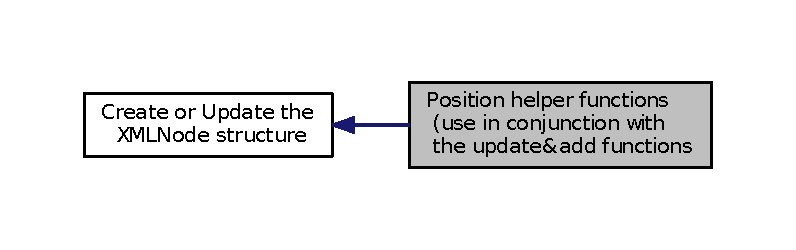
\includegraphics[width=350pt]{group__xmlPosition}
\end{center}
\end{figure}
\subsection*{Functions}
\begin{DoxyCompactItemize}
\item 
\hyperlink{xmlParser_8h_aab10d65aadeca1f026f6416becde7432}{X\-M\-L\-Element\-Position} \hyperlink{group__xmlPosition_ga4376524698201e37c805bfa37945a600}{X\-M\-L\-Node\-::position\-Of\-Text} (int i=0) const 
\item 
\hyperlink{xmlParser_8h_aab10d65aadeca1f026f6416becde7432}{X\-M\-L\-Element\-Position} \hyperlink{group__xmlPosition_ga3a590db071ce9f3fdc6e82405ab8507d}{X\-M\-L\-Node\-::position\-Of\-Text} (\hyperlink{xmlParser_8h_acdb0d6fd8dd596384b438d86cfb2b182}{X\-M\-L\-C\-S\-T\-R} lpsz\-Value) const 
\item 
\hyperlink{xmlParser_8h_aab10d65aadeca1f026f6416becde7432}{X\-M\-L\-Element\-Position} \hyperlink{group__xmlPosition_gafbeb4c6fcb5f164a4e5501d048c0f714}{X\-M\-L\-Node\-::position\-Of\-Clear} (int i=0) const 
\item 
\hyperlink{xmlParser_8h_aab10d65aadeca1f026f6416becde7432}{X\-M\-L\-Element\-Position} \hyperlink{group__xmlPosition_gaae9a760878f7e2d8e392b17edb00ea19}{X\-M\-L\-Node\-::position\-Of\-Clear} (\hyperlink{xmlParser_8h_acdb0d6fd8dd596384b438d86cfb2b182}{X\-M\-L\-C\-S\-T\-R} lpsz\-Value) const 
\item 
\hyperlink{xmlParser_8h_aab10d65aadeca1f026f6416becde7432}{X\-M\-L\-Element\-Position} \hyperlink{group__xmlPosition_ga917818941aa305d3829472d49f33a4b5}{X\-M\-L\-Node\-::position\-Of\-Clear} (\hyperlink{structXMLClear}{X\-M\-L\-Clear} $\ast$a) const 
\item 
\hyperlink{xmlParser_8h_aab10d65aadeca1f026f6416becde7432}{X\-M\-L\-Element\-Position} \hyperlink{group__xmlPosition_gac98af1de6ed1218e5d26f7e509b8678f}{X\-M\-L\-Node\-::position\-Of\-Child\-Node} (int i=0) const 
\item 
\hyperlink{xmlParser_8h_aab10d65aadeca1f026f6416becde7432}{X\-M\-L\-Element\-Position} \hyperlink{group__xmlPosition_gaf8457366bc393a57e33896e46592cb3e}{X\-M\-L\-Node\-::position\-Of\-Child\-Node} (\hyperlink{structXMLNode}{X\-M\-L\-Node} x) const 
\item 
\hyperlink{xmlParser_8h_aab10d65aadeca1f026f6416becde7432}{X\-M\-L\-Element\-Position} \hyperlink{group__xmlPosition_ga102dcd93d13144e2a87b664e6f810725}{X\-M\-L\-Node\-::position\-Of\-Child\-Node} (\hyperlink{xmlParser_8h_acdb0d6fd8dd596384b438d86cfb2b182}{X\-M\-L\-C\-S\-T\-R} name, int i=0) const 
\begin{DoxyCompactList}\small\item\em return the position of the ith child\-Node with the specified name if (name==N\-U\-L\-L) return the position of the ith child\-Node \end{DoxyCompactList}\end{DoxyCompactItemize}


\subsection{Detailed Description}
These are some useful functions when you want to insert a child\-Node, a text or a X\-M\-L\-Clear\-Tag in the middle (at a specified position) of a \hyperlink{structXMLNode}{X\-M\-L\-Node} tree already constructed. The value returned by these methods is to be used as last parameter (parameter 'pos') of add\-Child, add\-Text or add\-Clear. 

\subsection{Function Documentation}
\hypertarget{group__xmlPosition_gac98af1de6ed1218e5d26f7e509b8678f}{\index{Position helper functions (use in conjunction with the update\&add functions@{Position helper functions (use in conjunction with the update\&add functions}!position\-Of\-Child\-Node@{position\-Of\-Child\-Node}}
\index{position\-Of\-Child\-Node@{position\-Of\-Child\-Node}!Position helper functions (use in conjunction with the update&add functions@{Position helper functions (use in conjunction with the update\&add functions}}
\subsubsection[{position\-Of\-Child\-Node}]{\setlength{\rightskip}{0pt plus 5cm}{\bf X\-M\-L\-Element\-Position} X\-M\-L\-Node\-::position\-Of\-Child\-Node (
\begin{DoxyParamCaption}
\item[{int}]{i = {\ttfamily 0}}
\end{DoxyParamCaption}
) const}}\label{group__xmlPosition_gac98af1de6ed1218e5d26f7e509b8678f}
\hypertarget{group__xmlPosition_gaf8457366bc393a57e33896e46592cb3e}{\index{Position helper functions (use in conjunction with the update\&add functions@{Position helper functions (use in conjunction with the update\&add functions}!position\-Of\-Child\-Node@{position\-Of\-Child\-Node}}
\index{position\-Of\-Child\-Node@{position\-Of\-Child\-Node}!Position helper functions (use in conjunction with the update&add functions@{Position helper functions (use in conjunction with the update\&add functions}}
\subsubsection[{position\-Of\-Child\-Node}]{\setlength{\rightskip}{0pt plus 5cm}{\bf X\-M\-L\-Element\-Position} X\-M\-L\-Node\-::position\-Of\-Child\-Node (
\begin{DoxyParamCaption}
\item[{{\bf X\-M\-L\-Node}}]{x}
\end{DoxyParamCaption}
) const}}\label{group__xmlPosition_gaf8457366bc393a57e33896e46592cb3e}
\hypertarget{group__xmlPosition_ga102dcd93d13144e2a87b664e6f810725}{\index{Position helper functions (use in conjunction with the update\&add functions@{Position helper functions (use in conjunction with the update\&add functions}!position\-Of\-Child\-Node@{position\-Of\-Child\-Node}}
\index{position\-Of\-Child\-Node@{position\-Of\-Child\-Node}!Position helper functions (use in conjunction with the update&add functions@{Position helper functions (use in conjunction with the update\&add functions}}
\subsubsection[{position\-Of\-Child\-Node}]{\setlength{\rightskip}{0pt plus 5cm}{\bf X\-M\-L\-Element\-Position} X\-M\-L\-Node\-::position\-Of\-Child\-Node (
\begin{DoxyParamCaption}
\item[{{\bf X\-M\-L\-C\-S\-T\-R}}]{name, }
\item[{int}]{i = {\ttfamily 0}}
\end{DoxyParamCaption}
) const}}\label{group__xmlPosition_ga102dcd93d13144e2a87b664e6f810725}


return the position of the ith child\-Node with the specified name if (name==N\-U\-L\-L) return the position of the ith child\-Node 

\hypertarget{group__xmlPosition_gafbeb4c6fcb5f164a4e5501d048c0f714}{\index{Position helper functions (use in conjunction with the update\&add functions@{Position helper functions (use in conjunction with the update\&add functions}!position\-Of\-Clear@{position\-Of\-Clear}}
\index{position\-Of\-Clear@{position\-Of\-Clear}!Position helper functions (use in conjunction with the update&add functions@{Position helper functions (use in conjunction with the update\&add functions}}
\subsubsection[{position\-Of\-Clear}]{\setlength{\rightskip}{0pt plus 5cm}{\bf X\-M\-L\-Element\-Position} X\-M\-L\-Node\-::position\-Of\-Clear (
\begin{DoxyParamCaption}
\item[{int}]{i = {\ttfamily 0}}
\end{DoxyParamCaption}
) const}}\label{group__xmlPosition_gafbeb4c6fcb5f164a4e5501d048c0f714}
\hypertarget{group__xmlPosition_gaae9a760878f7e2d8e392b17edb00ea19}{\index{Position helper functions (use in conjunction with the update\&add functions@{Position helper functions (use in conjunction with the update\&add functions}!position\-Of\-Clear@{position\-Of\-Clear}}
\index{position\-Of\-Clear@{position\-Of\-Clear}!Position helper functions (use in conjunction with the update&add functions@{Position helper functions (use in conjunction with the update\&add functions}}
\subsubsection[{position\-Of\-Clear}]{\setlength{\rightskip}{0pt plus 5cm}{\bf X\-M\-L\-Element\-Position} X\-M\-L\-Node\-::position\-Of\-Clear (
\begin{DoxyParamCaption}
\item[{{\bf X\-M\-L\-C\-S\-T\-R}}]{lpsz\-Value}
\end{DoxyParamCaption}
) const}}\label{group__xmlPosition_gaae9a760878f7e2d8e392b17edb00ea19}
\hypertarget{group__xmlPosition_ga917818941aa305d3829472d49f33a4b5}{\index{Position helper functions (use in conjunction with the update\&add functions@{Position helper functions (use in conjunction with the update\&add functions}!position\-Of\-Clear@{position\-Of\-Clear}}
\index{position\-Of\-Clear@{position\-Of\-Clear}!Position helper functions (use in conjunction with the update&add functions@{Position helper functions (use in conjunction with the update\&add functions}}
\subsubsection[{position\-Of\-Clear}]{\setlength{\rightskip}{0pt plus 5cm}{\bf X\-M\-L\-Element\-Position} X\-M\-L\-Node\-::position\-Of\-Clear (
\begin{DoxyParamCaption}
\item[{{\bf X\-M\-L\-Clear} $\ast$}]{a}
\end{DoxyParamCaption}
) const}}\label{group__xmlPosition_ga917818941aa305d3829472d49f33a4b5}
\hypertarget{group__xmlPosition_ga4376524698201e37c805bfa37945a600}{\index{Position helper functions (use in conjunction with the update\&add functions@{Position helper functions (use in conjunction with the update\&add functions}!position\-Of\-Text@{position\-Of\-Text}}
\index{position\-Of\-Text@{position\-Of\-Text}!Position helper functions (use in conjunction with the update&add functions@{Position helper functions (use in conjunction with the update\&add functions}}
\subsubsection[{position\-Of\-Text}]{\setlength{\rightskip}{0pt plus 5cm}{\bf X\-M\-L\-Element\-Position} X\-M\-L\-Node\-::position\-Of\-Text (
\begin{DoxyParamCaption}
\item[{int}]{i = {\ttfamily 0}}
\end{DoxyParamCaption}
) const}}\label{group__xmlPosition_ga4376524698201e37c805bfa37945a600}
\hypertarget{group__xmlPosition_ga3a590db071ce9f3fdc6e82405ab8507d}{\index{Position helper functions (use in conjunction with the update\&add functions@{Position helper functions (use in conjunction with the update\&add functions}!position\-Of\-Text@{position\-Of\-Text}}
\index{position\-Of\-Text@{position\-Of\-Text}!Position helper functions (use in conjunction with the update&add functions@{Position helper functions (use in conjunction with the update\&add functions}}
\subsubsection[{position\-Of\-Text}]{\setlength{\rightskip}{0pt plus 5cm}{\bf X\-M\-L\-Element\-Position} X\-M\-L\-Node\-::position\-Of\-Text (
\begin{DoxyParamCaption}
\item[{{\bf X\-M\-L\-C\-S\-T\-R}}]{lpsz\-Value}
\end{DoxyParamCaption}
) const}}\label{group__xmlPosition_ga3a590db071ce9f3fdc6e82405ab8507d}

\hypertarget{group__StringAlloc}{\section{String Allocation/\-Free functions}
\label{group__StringAlloc}\index{String Allocation/\-Free functions@{String Allocation/\-Free functions}}
}
Collaboration diagram for String Allocation/\-Free functions\-:
\nopagebreak
\begin{figure}[H]
\begin{center}
\leavevmode
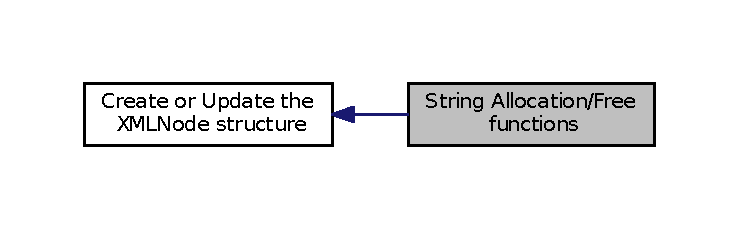
\includegraphics[width=350pt]{group__StringAlloc}
\end{center}
\end{figure}
\subsection*{Functions}
\begin{DoxyCompactItemize}
\item 
\hyperlink{xmlParser_8h_a990c86ec1cdbf675604a1a321d852063}{X\-M\-L\-D\-L\-L\-E\-N\-T\-R\-Y} \hyperlink{xmlParser_8h_a849d96105aa0c8f64b5c10d9151a3cdc}{X\-M\-L\-S\-T\-R} \hyperlink{group__StringAlloc_gac35b3be05a320f835b3976179637fe76}{string\-Dup} (\hyperlink{xmlParser_8h_acdb0d6fd8dd596384b438d86cfb2b182}{X\-M\-L\-C\-S\-T\-R} source, int cb\-Data=-\/1)
\begin{DoxyCompactList}\small\item\em Duplicate (copy in a new allocated buffer) the source string. \end{DoxyCompactList}\item 
\hyperlink{xmlParser_8h_a990c86ec1cdbf675604a1a321d852063}{X\-M\-L\-D\-L\-L\-E\-N\-T\-R\-Y} void \hyperlink{group__StringAlloc_ga6a510c9553d7fa49d0afdda1d7928669}{free\-X\-M\-L\-String} (\hyperlink{xmlParser_8h_a849d96105aa0c8f64b5c10d9151a3cdc}{X\-M\-L\-S\-T\-R} t)
\begin{DoxyCompactList}\small\item\em to free the string allocated inside the \char`\"{}string\-Dup\char`\"{} function or the \char`\"{}create\-X\-M\-L\-String\char`\"{} function. \end{DoxyCompactList}\end{DoxyCompactItemize}


\subsection{Detailed Description}


\subsection{Function Documentation}
\hypertarget{group__StringAlloc_ga6a510c9553d7fa49d0afdda1d7928669}{\index{String Allocation/\-Free functions@{String Allocation/\-Free functions}!free\-X\-M\-L\-String@{free\-X\-M\-L\-String}}
\index{free\-X\-M\-L\-String@{free\-X\-M\-L\-String}!String Allocation/Free functions@{String Allocation/\-Free functions}}
\subsubsection[{free\-X\-M\-L\-String}]{\setlength{\rightskip}{0pt plus 5cm}{\bf X\-M\-L\-D\-L\-L\-E\-N\-T\-R\-Y} void free\-X\-M\-L\-String (
\begin{DoxyParamCaption}
\item[{{\bf X\-M\-L\-S\-T\-R}}]{t}
\end{DoxyParamCaption}
)}}\label{group__StringAlloc_ga6a510c9553d7fa49d0afdda1d7928669}


to free the string allocated inside the \char`\"{}string\-Dup\char`\"{} function or the \char`\"{}create\-X\-M\-L\-String\char`\"{} function. 

\hypertarget{group__StringAlloc_gac35b3be05a320f835b3976179637fe76}{\index{String Allocation/\-Free functions@{String Allocation/\-Free functions}!string\-Dup@{string\-Dup}}
\index{string\-Dup@{string\-Dup}!String Allocation/Free functions@{String Allocation/\-Free functions}}
\subsubsection[{string\-Dup}]{\setlength{\rightskip}{0pt plus 5cm}{\bf X\-M\-L\-D\-L\-L\-E\-N\-T\-R\-Y} {\bf X\-M\-L\-S\-T\-R} string\-Dup (
\begin{DoxyParamCaption}
\item[{{\bf X\-M\-L\-C\-S\-T\-R}}]{source, }
\item[{int}]{cb\-Data = {\ttfamily -\/1}}
\end{DoxyParamCaption}
)}}\label{group__StringAlloc_gac35b3be05a320f835b3976179637fe76}


Duplicate (copy in a new allocated buffer) the source string. 

This is a very handy function when used with all the \char`\"{}\-X\-M\-L\-Node\-::$\ast$\-\_\-\-W\-O\-S\-D\char`\"{} functions (\hyperlink{group__xmlWOSD}{xml\-W\-O\-S\-D}). 
\begin{DoxyParams}{Parameters}
{\em cb\-Data} & If !=0 then cb\-Data is the number of chars to duplicate. New strings allocated with this function should be free'd using the \char`\"{}free\-X\-M\-L\-String\char`\"{} function. \\
\hline
{\em source} & \\
\hline
\end{DoxyParams}

\hypertarget{group__atoX}{\section{ato? like functions}
\label{group__atoX}\index{ato? like functions@{ato? like functions}}
}
Collaboration diagram for ato? like functions\-:
\nopagebreak
\begin{figure}[H]
\begin{center}
\leavevmode
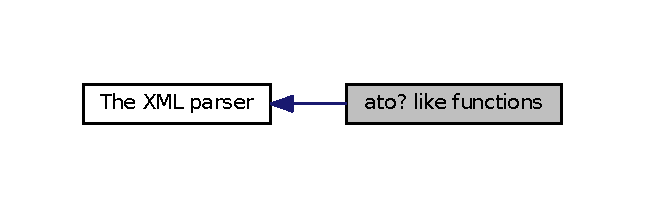
\includegraphics[width=310pt]{group__atoX}
\end{center}
\end{figure}
\subsection*{Functions}
\begin{DoxyCompactItemize}
\item 
\hyperlink{xmlParser_8h_a990c86ec1cdbf675604a1a321d852063}{X\-M\-L\-D\-L\-L\-E\-N\-T\-R\-Y} char \hyperlink{group__atoX_gac93e613b4563072bf7b43f91d2696c75}{xmltob} (\hyperlink{xmlParser_8h_acdb0d6fd8dd596384b438d86cfb2b182}{X\-M\-L\-C\-S\-T\-R} xml\-String, char defaut\-Value=0)
\item 
\hyperlink{xmlParser_8h_a990c86ec1cdbf675604a1a321d852063}{X\-M\-L\-D\-L\-L\-E\-N\-T\-R\-Y} int \hyperlink{group__atoX_ga17b00a11ddc49e8e253160cc56d6377f}{xmltoi} (\hyperlink{xmlParser_8h_acdb0d6fd8dd596384b438d86cfb2b182}{X\-M\-L\-C\-S\-T\-R} xml\-String, int defaut\-Value=0)
\item 
\hyperlink{xmlParser_8h_a990c86ec1cdbf675604a1a321d852063}{X\-M\-L\-D\-L\-L\-E\-N\-T\-R\-Y} long \hyperlink{group__atoX_gab69be88d6b554476470e7a1e6ec23589}{xmltol} (\hyperlink{xmlParser_8h_acdb0d6fd8dd596384b438d86cfb2b182}{X\-M\-L\-C\-S\-T\-R} xml\-String, long defaut\-Value=0)
\item 
\hyperlink{xmlParser_8h_a990c86ec1cdbf675604a1a321d852063}{X\-M\-L\-D\-L\-L\-E\-N\-T\-R\-Y} double \hyperlink{group__atoX_gaf820a1a0f8055c8e4a006a566be9500a}{xmltof} (\hyperlink{xmlParser_8h_acdb0d6fd8dd596384b438d86cfb2b182}{X\-M\-L\-C\-S\-T\-R} xml\-String, double defaut\-Value=.\-0)
\item 
\hyperlink{xmlParser_8h_a990c86ec1cdbf675604a1a321d852063}{X\-M\-L\-D\-L\-L\-E\-N\-T\-R\-Y} \hyperlink{xmlParser_8h_acdb0d6fd8dd596384b438d86cfb2b182}{X\-M\-L\-C\-S\-T\-R} \hyperlink{group__atoX_ga20998546f61a5d41ed3fe4553702473a}{xmltoa} (\hyperlink{xmlParser_8h_acdb0d6fd8dd596384b438d86cfb2b182}{X\-M\-L\-C\-S\-T\-R} xml\-String, \hyperlink{xmlParser_8h_acdb0d6fd8dd596384b438d86cfb2b182}{X\-M\-L\-C\-S\-T\-R} defaut\-Value=\hyperlink{xmlParser_8h_a17b1f4694ce8bdeef4c07319c5f8f84d}{\-\_\-\-C\-X\-M\-L}(\char`\"{}\char`\"{}))
\item 
\hyperlink{xmlParser_8h_a990c86ec1cdbf675604a1a321d852063}{X\-M\-L\-D\-L\-L\-E\-N\-T\-R\-Y} \hyperlink{xmlParser_8h_a9f587fbd233e721e8818a3bf8102838f}{X\-M\-L\-C\-H\-A\-R} \hyperlink{group__atoX_gaa929f34f436c3466e66196e5e2091e73}{xmltoc} (\hyperlink{xmlParser_8h_acdb0d6fd8dd596384b438d86cfb2b182}{X\-M\-L\-C\-S\-T\-R} xml\-String, const \hyperlink{xmlParser_8h_a9f587fbd233e721e8818a3bf8102838f}{X\-M\-L\-C\-H\-A\-R} defaut\-Value=\hyperlink{xmlParser_8h_a17b1f4694ce8bdeef4c07319c5f8f84d}{\-\_\-\-C\-X\-M\-L}('\textbackslash{}0'))
\end{DoxyCompactItemize}


\subsection{Detailed Description}
The \char`\"{}xmlto?\char`\"{} functions are equivalents to the atoi, atol, atof functions. The only difference is\-: If the variable \char`\"{}xml\-String\char`\"{} is N\-U\-L\-L, than the return value is \char`\"{}defaut\-Value\char`\"{}. These 6 functions are only here as \char`\"{}convenience\char`\"{} functions for the user (they are not used inside the X\-M\-Lparser). If you don't need them, you can delete them without any trouble. 

\subsection{Function Documentation}
\hypertarget{group__atoX_ga20998546f61a5d41ed3fe4553702473a}{\index{ato? like functions@{ato? like functions}!xmltoa@{xmltoa}}
\index{xmltoa@{xmltoa}!ato? like functions@{ato? like functions}}
\subsubsection[{xmltoa}]{\setlength{\rightskip}{0pt plus 5cm}{\bf X\-M\-L\-D\-L\-L\-E\-N\-T\-R\-Y} {\bf X\-M\-L\-C\-S\-T\-R} xmltoa (
\begin{DoxyParamCaption}
\item[{{\bf X\-M\-L\-C\-S\-T\-R}}]{xml\-String, }
\item[{{\bf X\-M\-L\-C\-S\-T\-R}}]{defaut\-Value = {\ttfamily {\bf \-\_\-\-C\-X\-M\-L}(\char`\"{}\char`\"{})}}
\end{DoxyParamCaption}
)}}\label{group__atoX_ga20998546f61a5d41ed3fe4553702473a}
\hypertarget{group__atoX_gac93e613b4563072bf7b43f91d2696c75}{\index{ato? like functions@{ato? like functions}!xmltob@{xmltob}}
\index{xmltob@{xmltob}!ato? like functions@{ato? like functions}}
\subsubsection[{xmltob}]{\setlength{\rightskip}{0pt plus 5cm}{\bf X\-M\-L\-D\-L\-L\-E\-N\-T\-R\-Y} char xmltob (
\begin{DoxyParamCaption}
\item[{{\bf X\-M\-L\-C\-S\-T\-R}}]{xml\-String, }
\item[{char}]{defaut\-Value = {\ttfamily 0}}
\end{DoxyParamCaption}
)}}\label{group__atoX_gac93e613b4563072bf7b43f91d2696c75}
\hypertarget{group__atoX_gaa929f34f436c3466e66196e5e2091e73}{\index{ato? like functions@{ato? like functions}!xmltoc@{xmltoc}}
\index{xmltoc@{xmltoc}!ato? like functions@{ato? like functions}}
\subsubsection[{xmltoc}]{\setlength{\rightskip}{0pt plus 5cm}{\bf X\-M\-L\-D\-L\-L\-E\-N\-T\-R\-Y} {\bf X\-M\-L\-C\-H\-A\-R} xmltoc (
\begin{DoxyParamCaption}
\item[{{\bf X\-M\-L\-C\-S\-T\-R}}]{xml\-String, }
\item[{const {\bf X\-M\-L\-C\-H\-A\-R}}]{defaut\-Value = {\ttfamily {\bf \-\_\-\-C\-X\-M\-L}('\textbackslash{}0')}}
\end{DoxyParamCaption}
)}}\label{group__atoX_gaa929f34f436c3466e66196e5e2091e73}
\hypertarget{group__atoX_gaf820a1a0f8055c8e4a006a566be9500a}{\index{ato? like functions@{ato? like functions}!xmltof@{xmltof}}
\index{xmltof@{xmltof}!ato? like functions@{ato? like functions}}
\subsubsection[{xmltof}]{\setlength{\rightskip}{0pt plus 5cm}{\bf X\-M\-L\-D\-L\-L\-E\-N\-T\-R\-Y} double xmltof (
\begin{DoxyParamCaption}
\item[{{\bf X\-M\-L\-C\-S\-T\-R}}]{xml\-String, }
\item[{double}]{defaut\-Value = {\ttfamily .0}}
\end{DoxyParamCaption}
)}}\label{group__atoX_gaf820a1a0f8055c8e4a006a566be9500a}
\hypertarget{group__atoX_ga17b00a11ddc49e8e253160cc56d6377f}{\index{ato? like functions@{ato? like functions}!xmltoi@{xmltoi}}
\index{xmltoi@{xmltoi}!ato? like functions@{ato? like functions}}
\subsubsection[{xmltoi}]{\setlength{\rightskip}{0pt plus 5cm}{\bf X\-M\-L\-D\-L\-L\-E\-N\-T\-R\-Y} int xmltoi (
\begin{DoxyParamCaption}
\item[{{\bf X\-M\-L\-C\-S\-T\-R}}]{xml\-String, }
\item[{int}]{defaut\-Value = {\ttfamily 0}}
\end{DoxyParamCaption}
)}}\label{group__atoX_ga17b00a11ddc49e8e253160cc56d6377f}
\hypertarget{group__atoX_gab69be88d6b554476470e7a1e6ec23589}{\index{ato? like functions@{ato? like functions}!xmltol@{xmltol}}
\index{xmltol@{xmltol}!ato? like functions@{ato? like functions}}
\subsubsection[{xmltol}]{\setlength{\rightskip}{0pt plus 5cm}{\bf X\-M\-L\-D\-L\-L\-E\-N\-T\-R\-Y} long xmltol (
\begin{DoxyParamCaption}
\item[{{\bf X\-M\-L\-C\-S\-T\-R}}]{xml\-String, }
\item[{long}]{defaut\-Value = {\ttfamily 0}}
\end{DoxyParamCaption}
)}}\label{group__atoX_gab69be88d6b554476470e7a1e6ec23589}

\hypertarget{group__ToXMLStringTool}{\section{Helper class to create X\-M\-L files using \char`\"{}printf\char`\"{}, \char`\"{}fprintf\char`\"{}, \char`\"{}cout\char`\"{},... functions.}
\label{group__ToXMLStringTool}\index{Helper class to create X\-M\-L files using \char`\"{}printf\char`\"{}, \char`\"{}fprintf\char`\"{}, \char`\"{}cout\char`\"{},... functions.@{Helper class to create X\-M\-L files using ""printf"", ""fprintf"", ""cout"",... functions.}}
}
Collaboration diagram for Helper class to create X\-M\-L files using \char`\"{}printf\char`\"{}, \char`\"{}fprintf\char`\"{}, \char`\"{}cout\char`\"{},... functions.\-:
\nopagebreak
\begin{figure}[H]
\begin{center}
\leavevmode
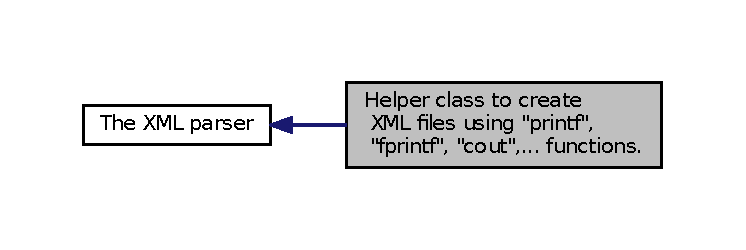
\includegraphics[width=350pt]{group__ToXMLStringTool}
\end{center}
\end{figure}
\subsection*{Classes}
\begin{DoxyCompactItemize}
\item 
struct \hyperlink{structToXMLStringTool}{To\-X\-M\-L\-String\-Tool}
\begin{DoxyCompactList}\small\item\em Helper class to create X\-M\-L files using \char`\"{}printf\char`\"{}, \char`\"{}fprintf\char`\"{}, \char`\"{}cout\char`\"{},... functions. \end{DoxyCompactList}\end{DoxyCompactItemize}
\subsection*{Typedefs}
\begin{DoxyCompactItemize}
\item 
typedef struct \hyperlink{xmlParser_8h_a990c86ec1cdbf675604a1a321d852063}{X\-M\-L\-D\-L\-L\-E\-N\-T\-R\-Y} \\*
\hyperlink{structToXMLStringTool}{To\-X\-M\-L\-String\-Tool} \hyperlink{group__ToXMLStringTool_ga0460d731addf12b0863d4fd857ca8281}{To\-X\-M\-L\-String\-Tool}
\begin{DoxyCompactList}\small\item\em Helper class to create X\-M\-L files using \char`\"{}printf\char`\"{}, \char`\"{}fprintf\char`\"{}, \char`\"{}cout\char`\"{},... functions. \end{DoxyCompactList}\end{DoxyCompactItemize}


\subsection{Detailed Description}


\subsection{Typedef Documentation}
\hypertarget{group__ToXMLStringTool_ga0460d731addf12b0863d4fd857ca8281}{\index{Helper class to create X\-M\-L files using \char`\"{}printf\char`\"{}, \char`\"{}fprintf\char`\"{}, \char`\"{}cout\char`\"{},... functions.@{Helper class to create X\-M\-L files using ""printf"", ""fprintf"", ""cout"",... functions.}!To\-X\-M\-L\-String\-Tool@{To\-X\-M\-L\-String\-Tool}}
\index{To\-X\-M\-L\-String\-Tool@{To\-X\-M\-L\-String\-Tool}!Helper class to create XML files using "printf", "fprintf", "cout",... functions.@{Helper class to create X\-M\-L files using \char`\"{}printf\char`\"{}, \char`\"{}fprintf\char`\"{}, \char`\"{}cout\char`\"{},... functions.}}
\subsubsection[{To\-X\-M\-L\-String\-Tool}]{\setlength{\rightskip}{0pt plus 5cm}typedef struct {\bf X\-M\-L\-D\-L\-L\-E\-N\-T\-R\-Y} {\bf To\-X\-M\-L\-String\-Tool}  {\bf To\-X\-M\-L\-String\-Tool}}}\label{group__ToXMLStringTool_ga0460d731addf12b0863d4fd857ca8281}


Helper class to create X\-M\-L files using \char`\"{}printf\char`\"{}, \char`\"{}fprintf\char`\"{}, \char`\"{}cout\char`\"{},... functions. 

The \hyperlink{structToXMLStringTool}{To\-X\-M\-L\-String\-Tool} class helps you creating X\-M\-L files using \char`\"{}printf\char`\"{}, \char`\"{}fprintf\char`\"{}, \char`\"{}cout\char`\"{},... functions. The \char`\"{}\-To\-X\-M\-L\-String\-Tool\char`\"{} class is processing strings so that all the characters \&,",',$<$,$>$ are replaced by their X\-M\-L equivalent\-: \begin{DoxyVerb}&amp;, &quot;, &apos;, &lt;, &gt; \end{DoxyVerb}
 Using the \char`\"{}\-To\-X\-M\-L\-String\-Tool class\char`\"{} and the \char`\"{}fprintf function\char`\"{} is T\-H\-E most efficient way to produce V\-E\-R\-Y large X\-M\-L documents V\-E\-R\-Y fast. \begin{DoxyNote}{Note}
If you are creating from scratch an X\-M\-L file using the provided \hyperlink{structXMLNode}{X\-M\-L\-Node} class you must not use the \char`\"{}\-To\-X\-M\-L\-String\-Tool\char`\"{} class (because the \char`\"{}\-X\-M\-L\-Node\char`\"{} class does the processing job for you during rendering). 
\end{DoxyNote}

\hypertarget{group__XMLParserBase64Tool}{\section{Helper class to include binary data inside X\-M\-L strings using \char`\"{}\-Base64 encoding\char`\"{}.}
\label{group__XMLParserBase64Tool}\index{Helper class to include binary data inside X\-M\-L strings using \char`\"{}\-Base64 encoding\char`\"{}.@{Helper class to include binary data inside X\-M\-L strings using ""Base64 encoding"".}}
}
Collaboration diagram for Helper class to include binary data inside X\-M\-L strings using \char`\"{}\-Base64 encoding\char`\"{}.\-:
\nopagebreak
\begin{figure}[H]
\begin{center}
\leavevmode
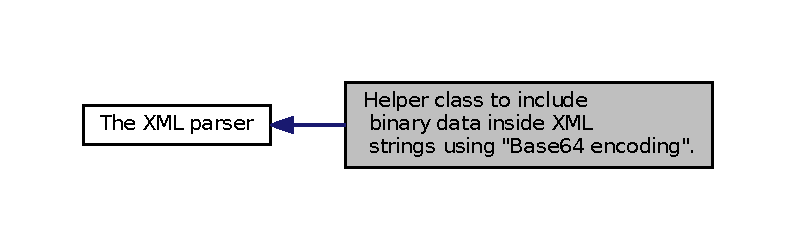
\includegraphics[width=350pt]{group__XMLParserBase64Tool}
\end{center}
\end{figure}
\subsection*{Classes}
\begin{DoxyCompactItemize}
\item 
struct \hyperlink{structXMLParserBase64Tool}{X\-M\-L\-Parser\-Base64\-Tool}
\begin{DoxyCompactList}\small\item\em Helper class to include binary data inside X\-M\-L strings using \char`\"{}\-Base64 encoding\char`\"{}. \end{DoxyCompactList}\end{DoxyCompactItemize}
\subsection*{Typedefs}
\begin{DoxyCompactItemize}
\item 
typedef struct \hyperlink{xmlParser_8h_a990c86ec1cdbf675604a1a321d852063}{X\-M\-L\-D\-L\-L\-E\-N\-T\-R\-Y} \\*
\hyperlink{structXMLParserBase64Tool}{X\-M\-L\-Parser\-Base64\-Tool} \hyperlink{group__XMLParserBase64Tool_ga90d0646ff4a054f9d8ea0d29fb86f3a9}{X\-M\-L\-Parser\-Base64\-Tool}
\begin{DoxyCompactList}\small\item\em Helper class to include binary data inside X\-M\-L strings using \char`\"{}\-Base64 encoding\char`\"{}. \end{DoxyCompactList}\end{DoxyCompactItemize}


\subsection{Detailed Description}


\subsection{Typedef Documentation}
\hypertarget{group__XMLParserBase64Tool_ga90d0646ff4a054f9d8ea0d29fb86f3a9}{\index{Helper class to include binary data inside X\-M\-L strings using \char`\"{}\-Base64 encoding\char`\"{}.@{Helper class to include binary data inside X\-M\-L strings using ""Base64 encoding"".}!X\-M\-L\-Parser\-Base64\-Tool@{X\-M\-L\-Parser\-Base64\-Tool}}
\index{X\-M\-L\-Parser\-Base64\-Tool@{X\-M\-L\-Parser\-Base64\-Tool}!Helper class to include binary data inside XML strings using "Base64 encoding".@{Helper class to include binary data inside X\-M\-L strings using \char`\"{}\-Base64 encoding\char`\"{}.}}
\subsubsection[{X\-M\-L\-Parser\-Base64\-Tool}]{\setlength{\rightskip}{0pt plus 5cm}typedef struct {\bf X\-M\-L\-D\-L\-L\-E\-N\-T\-R\-Y} {\bf X\-M\-L\-Parser\-Base64\-Tool} {\bf X\-M\-L\-Parser\-Base64\-Tool}}}\label{group__XMLParserBase64Tool_ga90d0646ff4a054f9d8ea0d29fb86f3a9}


Helper class to include binary data inside X\-M\-L strings using \char`\"{}\-Base64 encoding\char`\"{}. 

The \char`\"{}\-X\-M\-L\-Parser\-Base64\-Tool\char`\"{} class allows you to include any binary data (images, sounds,...) into an X\-M\-L document using \char`\"{}\-Base64 encoding\char`\"{}. This class is completely separated from the rest of the xml\-Parser library and can be removed without any problem. To include some binary data into an X\-M\-L file, you must convert the binary data into standard text (using \char`\"{}encode\char`\"{}). To retrieve the original binary data from the b64-\/encoded text included inside the X\-M\-L file, use \char`\"{}decode\char`\"{}. Alternatively, these functions can also be used to \char`\"{}encrypt/decrypt\char`\"{} some critical data contained inside the X\-M\-L (it's not a strong encryption at all, but sometimes it can be useful). 
\chapter{Namespace Documentation}
\hypertarget{namespaceunisys}{\section{unisys Namespace Reference}
\label{namespaceunisys}\index{unisys@{unisys}}
}


This namespace.  


\subsection*{Classes}
\begin{DoxyCompactItemize}
\item 
class \hyperlink{classunisys_1_1Database}{Database}
\begin{DoxyCompactList}\small\item\em This class is a database handle class. \end{DoxyCompactList}\item 
class \hyperlink{classunisys_1_1Query}{Query}
\item 
class \hyperlink{classunisys_1_1Updater}{Updater}
\item 
class \hyperlink{classunisys_1_1BatchInsert}{Batch\-Insert}
\item 
class \hyperlink{classunisys_1_1DataObj}{Data\-Obj}
\item 
class \hyperlink{classunisys_1_1Miriam}{Miriam}
\begin{DoxyCompactList}\small\item\em This class is for miriam cross reference annotation. \end{DoxyCompactList}\item 
class \hyperlink{classunisys_1_1IdRef}{Id\-Ref}
\begin{DoxyCompactList}\small\item\em Identifier reference class. \end{DoxyCompactList}\item 
class \hyperlink{classunisys_1_1PEIdRef}{P\-E\-Id\-Ref}
\begin{DoxyCompactList}\small\item\em Identifier reference class specific to physicalentity collection namespace. \end{DoxyCompactList}\item 
class \hyperlink{classunisys_1_1IntIdRef}{Int\-Id\-Ref}
\begin{DoxyCompactList}\small\item\em Identifier reference class specific to Iinteraction collection namespace. \end{DoxyCompactList}\item 
class \hyperlink{classunisys_1_1OntoIdRef}{Onto\-Id\-Ref}
\begin{DoxyCompactList}\small\item\em Identifier reference class specific to obo collection namespace. \end{DoxyCompactList}\item 
class \hyperlink{classunisys_1_1Tracking}{Tracking}
\begin{DoxyCompactList}\small\item\em Data updating history class. \end{DoxyCompactList}\item 
class \hyperlink{classunisys_1_1LiteralBSON}{Literal\-B\-S\-O\-N}
\begin{DoxyCompactList}\small\item\em Specific B\-S\-O\-N object to manage general \hyperlink{classunisys_1_1Literal}{Literal} data object. \end{DoxyCompactList}\item 
class \hyperlink{classunisys_1_1Literal}{Literal}
\begin{DoxyCompactList}\small\item\em \hyperlink{classunisys_1_1Literal}{Literal} class. \end{DoxyCompactList}\item 
class \hyperlink{classunisys_1_1Xref}{Xref}
\begin{DoxyCompactList}\small\item\em The C++ representative class for Cross reference data class. \end{DoxyCompactList}\item 
class \hyperlink{classunisys_1_1Score}{Score}
\begin{DoxyCompactList}\small\item\em The C++ representative class for \hyperlink{classunisys_1_1Score}{Score} class in data structure. \end{DoxyCompactList}\item 
class \hyperlink{classunisys_1_1BioSource}{Bio\-Source}
\begin{DoxyCompactList}\small\item\em The C++ representative class for Biological Source data class. This class is designed to manage the biological data of source organism. \end{DoxyCompactList}\item 
class \hyperlink{classunisys_1_1Evidence}{Evidence}
\begin{DoxyCompactList}\small\item\em The C++ representative class for evidence data class. \end{DoxyCompactList}\item 
class \hyperlink{classunisys_1_1Annotation}{Annotation}
\begin{DoxyCompactList}\small\item\em The C++ representative class for annotation data class. \end{DoxyCompactList}\item 
class \hyperlink{classunisys_1_1OntoRelationship}{Onto\-Relationship}
\begin{DoxyCompactList}\small\item\em The C++ representative class for relationship data class. \end{DoxyCompactList}\item 
class \hyperlink{classunisys_1_1Relation}{Relation}
\begin{DoxyCompactList}\small\item\em The C++ representative class for relationship data class. \end{DoxyCompactList}\item 
class \hyperlink{classunisys_1_1CellularLocation}{Cellular\-Location}
\begin{DoxyCompactList}\small\item\em The C++ representative class for cellular location data class. \end{DoxyCompactList}\item 
class \hyperlink{classunisys_1_1MathML}{Math\-M\-L}
\begin{DoxyCompactList}\small\item\em The C++ representative class for \hyperlink{classunisys_1_1MathML}{Math\-M\-L} data class. \end{DoxyCompactList}\item 
class \hyperlink{classunisys_1_1KineticParameter}{Kinetic\-Parameter}
\begin{DoxyCompactList}\small\item\em The C++ representative class for kinetic parameter data class. \end{DoxyCompactList}\item 
class \hyperlink{classunisys_1_1SubRegion}{Sub\-Region}
\begin{DoxyCompactList}\small\item\em The C++ representative class for sub-\/region data class. \end{DoxyCompactList}\item 
class \hyperlink{classunisys_1_1Metadata}{Metadata}
\begin{DoxyCompactList}\small\item\em The C++ representative class for metadata data class. \end{DoxyCompactList}\item 
class \hyperlink{classunisys_1_1Object}{Object}
\begin{DoxyCompactList}\small\item\em Root of all object classes This class does not have any interfaces. \end{DoxyCompactList}\item 
class \hyperlink{classunisys_1_1Ontology}{Ontology}
\begin{DoxyCompactList}\small\item\em \hyperlink{classunisys_1_1Ontology}{Ontology} data class. \end{DoxyCompactList}\item 
class \hyperlink{classunisys_1_1BioObject}{Bio\-Object}
\begin{DoxyCompactList}\small\item\em This class is for miriam cross reference annotation. \end{DoxyCompactList}\item 
class \hyperlink{classunisys_1_1PhysicalEntity}{Physical\-Entity}
\begin{DoxyCompactList}\small\item\em This class is for miriam cross reference annotation. \end{DoxyCompactList}\item 
class \hyperlink{classunisys_1_1SmallMolecule}{Small\-Molecule}
\begin{DoxyCompactList}\small\item\em This class is for miriam cross reference annotation. \end{DoxyCompactList}\item 
class \hyperlink{classunisys_1_1DNA}{D\-N\-A}
\begin{DoxyCompactList}\small\item\em This class is for miriam cross reference annotation. \end{DoxyCompactList}\item 
class \hyperlink{classunisys_1_1DNARegion}{D\-N\-A\-Region}
\begin{DoxyCompactList}\small\item\em This class is for miriam cross reference annotation. \end{DoxyCompactList}\item 
class \hyperlink{classunisys_1_1RNA}{R\-N\-A}
\begin{DoxyCompactList}\small\item\em This class is for miriam cross reference annotation. \end{DoxyCompactList}\item 
class \hyperlink{classunisys_1_1Protein}{Protein}
\begin{DoxyCompactList}\small\item\em This class is for miriam cross reference annotation. \end{DoxyCompactList}\item 
class \hyperlink{classunisys_1_1Complex}{Complex}
\begin{DoxyCompactList}\small\item\em This class is for miriam cross reference annotation. \end{DoxyCompactList}\item 
class \hyperlink{classunisys_1_1Interaction}{Interaction}
\begin{DoxyCompactList}\small\item\em This class is for miriam cross reference annotation. \end{DoxyCompactList}\item 
class \hyperlink{classunisys_1_1Control}{Control}
\begin{DoxyCompactList}\small\item\em This class is for miriam cross reference annotation. \end{DoxyCompactList}\item 
class \hyperlink{classunisys_1_1MolecularInteraction}{Molecular\-Interaction}
\begin{DoxyCompactList}\small\item\em This class is for miriam cross reference annotation. \end{DoxyCompactList}\item 
class \hyperlink{classunisys_1_1GeneticInteraction}{Genetic\-Interaction}
\begin{DoxyCompactList}\small\item\em This class is for miriam cross reference annotation. \end{DoxyCompactList}\item 
class \hyperlink{classunisys_1_1Conversion}{Conversion}
\begin{DoxyCompactList}\small\item\em This class is for miriam cross reference annotation. \end{DoxyCompactList}\item 
class \hyperlink{classunisys_1_1BiochemicalReaction}{Biochemical\-Reaction}
\begin{DoxyCompactList}\small\item\em This class is for miriam cross reference annotation. \end{DoxyCompactList}\item 
class \hyperlink{classunisys_1_1Transport}{Transport}
\begin{DoxyCompactList}\small\item\em This class is for miriam cross reference annotation. \end{DoxyCompactList}\item 
class \hyperlink{classunisys_1_1BiochemicalReactionWithTransport}{Biochemical\-Reaction\-With\-Transport}
\begin{DoxyCompactList}\small\item\em This class is for miriam cross reference annotation. \end{DoxyCompactList}\item 
class \hyperlink{classunisys_1_1UniSysError}{Uni\-Sys\-Error}
\item 
class \hyperlink{classunisys_1_1ConnectionError}{Connection\-Error}
\item 
class \hyperlink{classunisys_1_1UpdateError}{Update\-Error}
\item 
class \hyperlink{classunisys_1_1QueryError}{Query\-Error}
\item 
class \hyperlink{classunisys_1_1DataError}{Data\-Error}
\item 
class \hyperlink{classunisys_1_1ParsingError}{Parsing\-Error}
\item 
class \hyperlink{classunisys_1_1RESTServiceError}{R\-E\-S\-T\-Service\-Error}
\item 
class \hyperlink{classunisys_1_1BIOPAX__obj}{B\-I\-O\-P\-A\-X\-\_\-obj}
\begin{DoxyCompactList}\small\item\em This class is used to parse O\-W\-L format. \end{DoxyCompactList}\item 
class \hyperlink{classunisys_1_1BIOPAX2}{B\-I\-O\-P\-A\-X2}
\begin{DoxyCompactList}\small\item\em This class is used to parse O\-W\-L format. \end{DoxyCompactList}\item 
class \hyperlink{classunisys_1_1ChEBIOWLClass}{Ch\-E\-B\-I\-O\-W\-L\-Class}
\begin{DoxyCompactList}\small\item\em To handle owl\-:class tag of Ch\-E\-B\-I O\-W\-L format. \end{DoxyCompactList}\item 
class \hyperlink{classunisys_1_1ChEBIOWL}{Ch\-E\-B\-I\-O\-W\-L}
\begin{DoxyCompactList}\small\item\em Used to parse Ch\-E\-B\-I O\-W\-L format. \end{DoxyCompactList}\item 
class \hyperlink{classunisys_1_1Stanza}{Stanza}
\begin{DoxyCompactList}\small\item\em This class is used to parse O\-W\-L format. \end{DoxyCompactList}\item 
class \hyperlink{classunisys_1_1OBOXML}{O\-B\-O\-X\-M\-L}
\begin{DoxyCompactList}\small\item\em This class is used to parse O\-W\-L format. \end{DoxyCompactList}\item 
class \hyperlink{classunisys_1_1PSIMI}{P\-S\-I\-M\-I}
\begin{DoxyCompactList}\small\item\em A \hyperlink{classunisys_1_1PSIMI}{P\-S\-I\-M\-I} class is used for a data in P\-S\-I-\/\-M\-I X\-M\-L2.\-5 file format. \end{DoxyCompactList}\item 
class \hyperlink{classunisys_1_1RestBioMartResult}{Rest\-Bio\-Mart\-Result}
\begin{DoxyCompactList}\small\item\em General class for taking care the response from Bio\-Portal's \hyperlink{classunisys_1_1REST}{R\-E\-S\-T} service. \end{DoxyCompactList}\item 
class \hyperlink{classunisys_1_1RestBioMart}{Rest\-Bio\-Mart}
\begin{DoxyCompactList}\small\item\em General class for taking care the response from Bio\-Portal's \hyperlink{classunisys_1_1REST}{R\-E\-S\-T} service. \end{DoxyCompactList}\item 
class \hyperlink{classunisys_1_1RestBioPortalResult}{Rest\-Bio\-Portal\-Result}
\begin{DoxyCompactList}\small\item\em General class for taking care the response from Bio\-Portal's \hyperlink{classunisys_1_1REST}{R\-E\-S\-T} service. \end{DoxyCompactList}\item 
class \hyperlink{classunisys_1_1RestBioPortalSearchResult}{Rest\-Bio\-Portal\-Search\-Result}
\begin{DoxyCompactList}\small\item\em General class for taking care the response from Bio\-Portal's search command of \hyperlink{classunisys_1_1REST}{R\-E\-S\-T} service. \end{DoxyCompactList}\item 
class \hyperlink{classunisys_1_1ClassBean}{Class\-Bean}
\begin{DoxyCompactList}\small\item\em This class is for taking care of the specific structure of response data call class\-Bean. \end{DoxyCompactList}\item 
class \hyperlink{classunisys_1_1RestBioPortalTermResult}{Rest\-Bio\-Portal\-Term\-Result}
\begin{DoxyCompactList}\small\item\em This class is for parsing the response of term command. \end{DoxyCompactList}\item 
class \hyperlink{classunisys_1_1RestBioPortal}{Rest\-Bio\-Portal}
\begin{DoxyCompactList}\small\item\em The main class of Bio\-Portal \hyperlink{classunisys_1_1REST}{R\-E\-S\-T} service library. \end{DoxyCompactList}\item 
class \hyperlink{classunisys_1_1RestMiriam}{Rest\-Miriam}
\begin{DoxyCompactList}\small\item\em General class for taking care the response from Bio\-Portal's \hyperlink{classunisys_1_1REST}{R\-E\-S\-T} service. \end{DoxyCompactList}\item 
class \hyperlink{classunisys_1_1REST}{R\-E\-S\-T}
\begin{DoxyCompactList}\small\item\em Used for managing the request and response of \hyperlink{classunisys_1_1REST}{R\-E\-S\-T} service. \end{DoxyCompactList}\end{DoxyCompactItemize}
\subsection*{Enumerations}
\begin{DoxyCompactItemize}
\item 
enum \hyperlink{namespaceunisys_a06abbe485d59787061d5a0ab762a0bf5}{db\-Status} \{ \hyperlink{namespaceunisys_a06abbe485d59787061d5a0ab762a0bf5acb3b534f7025edd0c02c492398b57db7}{D\-B\-\_\-\-O\-K}, 
\hyperlink{namespaceunisys_a06abbe485d59787061d5a0ab762a0bf5a2b0cce7d96d864ec36448039d4a9d85f}{D\-B\-\_\-\-C\-A\-N\-N\-O\-T\-\_\-\-C\-O\-N\-N\-E\-C\-T}, 
\hyperlink{namespaceunisys_a06abbe485d59787061d5a0ab762a0bf5a793c9ad562d8f9cea7dd4dcc93bc957a}{D\-B\-\_\-\-C\-A\-N\-N\-O\-T\-\_\-\-I\-N\-S\-E\-R\-T}
 \}
\end{DoxyCompactItemize}
\subsection*{Functions}
\begin{DoxyCompactItemize}
\item 
std\-::string \hyperlink{namespaceunisys_a34d383680495fae6b5cfa615ef4e234b}{set\-Miriam\-U\-R\-N} (std\-::string db, \hyperlink{structXMLNode}{X\-M\-L\-Node} node)
\item 
{\footnotesize template$<$class type $>$ }\\mongo\-::\-B\-S\-O\-N\-Array \hyperlink{namespaceunisys_ab99d42c514d40e0a3752a9d97e8049f6}{to\-B\-S\-O\-N\-Array} (type const \&input)
\item 
{\footnotesize template$<$class type $>$ }\\std\-::set$<$ type $>$ \hyperlink{namespaceunisys_a3fcaf2bd3c84c1169b4d7771ad49520b}{B\-S\-O\-N\-To\-Set} (mongo\-::\-B\-S\-O\-N\-Obj const \&bson\-Obj)
\item 
{\footnotesize template$<$class type $>$ }\\std\-::vector$<$ type $>$ \hyperlink{namespaceunisys_a9f6f070f7120ff13e625fe438dc14dea}{B\-S\-O\-N\-To\-Vector} (mongo\-::\-B\-S\-O\-N\-Obj const \&bson\-Obj)
\end{DoxyCompactItemize}


\subsection{Detailed Description}
This namespace. some description. 

\subsection{Enumeration Type Documentation}
\hypertarget{namespaceunisys_a06abbe485d59787061d5a0ab762a0bf5}{\index{unisys@{unisys}!db\-Status@{db\-Status}}
\index{db\-Status@{db\-Status}!unisys@{unisys}}
\subsubsection[{db\-Status}]{\setlength{\rightskip}{0pt plus 5cm}enum {\bf unisys\-::db\-Status}}}\label{namespaceunisys_a06abbe485d59787061d5a0ab762a0bf5}
\begin{Desc}
\item[Enumerator\-: ]\par
\begin{description}
\index{D\-B\-\_\-\-O\-K@{D\-B\-\_\-\-O\-K}!unisys@{unisys}}\index{unisys@{unisys}!D\-B\-\_\-\-O\-K@{D\-B\-\_\-\-O\-K}}\item[{\em 
\hypertarget{namespaceunisys_a06abbe485d59787061d5a0ab762a0bf5acb3b534f7025edd0c02c492398b57db7}{D\-B\-\_\-\-O\-K}\label{namespaceunisys_a06abbe485d59787061d5a0ab762a0bf5acb3b534f7025edd0c02c492398b57db7}
}]\index{D\-B\-\_\-\-C\-A\-N\-N\-O\-T\-\_\-\-C\-O\-N\-N\-E\-C\-T@{D\-B\-\_\-\-C\-A\-N\-N\-O\-T\-\_\-\-C\-O\-N\-N\-E\-C\-T}!unisys@{unisys}}\index{unisys@{unisys}!D\-B\-\_\-\-C\-A\-N\-N\-O\-T\-\_\-\-C\-O\-N\-N\-E\-C\-T@{D\-B\-\_\-\-C\-A\-N\-N\-O\-T\-\_\-\-C\-O\-N\-N\-E\-C\-T}}\item[{\em 
\hypertarget{namespaceunisys_a06abbe485d59787061d5a0ab762a0bf5a2b0cce7d96d864ec36448039d4a9d85f}{D\-B\-\_\-\-C\-A\-N\-N\-O\-T\-\_\-\-C\-O\-N\-N\-E\-C\-T}\label{namespaceunisys_a06abbe485d59787061d5a0ab762a0bf5a2b0cce7d96d864ec36448039d4a9d85f}
}]\index{D\-B\-\_\-\-C\-A\-N\-N\-O\-T\-\_\-\-I\-N\-S\-E\-R\-T@{D\-B\-\_\-\-C\-A\-N\-N\-O\-T\-\_\-\-I\-N\-S\-E\-R\-T}!unisys@{unisys}}\index{unisys@{unisys}!D\-B\-\_\-\-C\-A\-N\-N\-O\-T\-\_\-\-I\-N\-S\-E\-R\-T@{D\-B\-\_\-\-C\-A\-N\-N\-O\-T\-\_\-\-I\-N\-S\-E\-R\-T}}\item[{\em 
\hypertarget{namespaceunisys_a06abbe485d59787061d5a0ab762a0bf5a793c9ad562d8f9cea7dd4dcc93bc957a}{D\-B\-\_\-\-C\-A\-N\-N\-O\-T\-\_\-\-I\-N\-S\-E\-R\-T}\label{namespaceunisys_a06abbe485d59787061d5a0ab762a0bf5a793c9ad562d8f9cea7dd4dcc93bc957a}
}]\end{description}
\end{Desc}



\subsection{Function Documentation}
\hypertarget{namespaceunisys_a3fcaf2bd3c84c1169b4d7771ad49520b}{\index{unisys@{unisys}!B\-S\-O\-N\-To\-Set@{B\-S\-O\-N\-To\-Set}}
\index{B\-S\-O\-N\-To\-Set@{B\-S\-O\-N\-To\-Set}!unisys@{unisys}}
\subsubsection[{B\-S\-O\-N\-To\-Set}]{\setlength{\rightskip}{0pt plus 5cm}template$<$class type $>$ std\-::set$<$type$>$ unisys\-::\-B\-S\-O\-N\-To\-Set (
\begin{DoxyParamCaption}
\item[{mongo\-::\-B\-S\-O\-N\-Obj const \&}]{bson\-Obj}
\end{DoxyParamCaption}
)}}\label{namespaceunisys_a3fcaf2bd3c84c1169b4d7771ad49520b}
\hypertarget{namespaceunisys_a9f6f070f7120ff13e625fe438dc14dea}{\index{unisys@{unisys}!B\-S\-O\-N\-To\-Vector@{B\-S\-O\-N\-To\-Vector}}
\index{B\-S\-O\-N\-To\-Vector@{B\-S\-O\-N\-To\-Vector}!unisys@{unisys}}
\subsubsection[{B\-S\-O\-N\-To\-Vector}]{\setlength{\rightskip}{0pt plus 5cm}template$<$class type $>$ std\-::vector$<$type$>$ unisys\-::\-B\-S\-O\-N\-To\-Vector (
\begin{DoxyParamCaption}
\item[{mongo\-::\-B\-S\-O\-N\-Obj const \&}]{bson\-Obj}
\end{DoxyParamCaption}
)}}\label{namespaceunisys_a9f6f070f7120ff13e625fe438dc14dea}
\hypertarget{namespaceunisys_a34d383680495fae6b5cfa615ef4e234b}{\index{unisys@{unisys}!set\-Miriam\-U\-R\-N@{set\-Miriam\-U\-R\-N}}
\index{set\-Miriam\-U\-R\-N@{set\-Miriam\-U\-R\-N}!unisys@{unisys}}
\subsubsection[{set\-Miriam\-U\-R\-N}]{\setlength{\rightskip}{0pt plus 5cm}std\-::string unisys\-::set\-Miriam\-U\-R\-N (
\begin{DoxyParamCaption}
\item[{std\-::string}]{db, }
\item[{{\bf X\-M\-L\-Node}}]{node}
\end{DoxyParamCaption}
)}}\label{namespaceunisys_a34d383680495fae6b5cfa615ef4e234b}
\hypertarget{namespaceunisys_ab99d42c514d40e0a3752a9d97e8049f6}{\index{unisys@{unisys}!to\-B\-S\-O\-N\-Array@{to\-B\-S\-O\-N\-Array}}
\index{to\-B\-S\-O\-N\-Array@{to\-B\-S\-O\-N\-Array}!unisys@{unisys}}
\subsubsection[{to\-B\-S\-O\-N\-Array}]{\setlength{\rightskip}{0pt plus 5cm}template$<$class type $>$ mongo\-::\-B\-S\-O\-N\-Array unisys\-::to\-B\-S\-O\-N\-Array (
\begin{DoxyParamCaption}
\item[{type const \&}]{input}
\end{DoxyParamCaption}
)}}\label{namespaceunisys_ab99d42c514d40e0a3752a9d97e8049f6}

\chapter{Class Documentation}
\hypertarget{classunisys_1_1Annotation}{\section{unisys\-:\-:Annotation Class Reference}
\label{classunisys_1_1Annotation}\index{unisys\-::\-Annotation@{unisys\-::\-Annotation}}
}


The C++ representative class for annotation data class.  




{\ttfamily \#include $<$Lit\-Class.\-h$>$}



Inheritance diagram for unisys\-:\-:Annotation\-:
\nopagebreak
\begin{figure}[H]
\begin{center}
\leavevmode
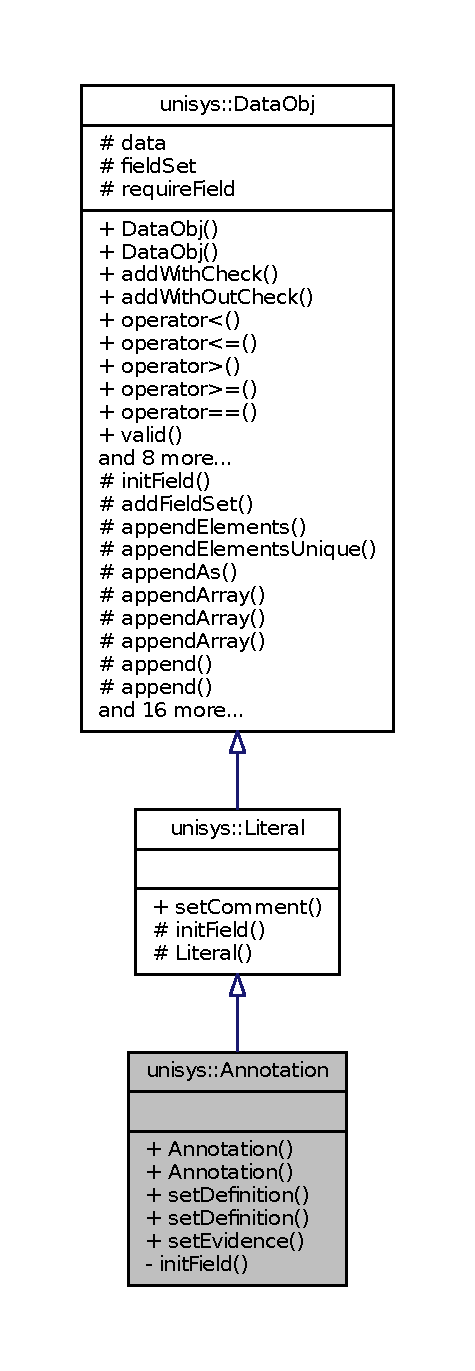
\includegraphics[height=550pt]{classunisys_1_1Annotation__inherit__graph}
\end{center}
\end{figure}


Collaboration diagram for unisys\-:\-:Annotation\-:
\nopagebreak
\begin{figure}[H]
\begin{center}
\leavevmode
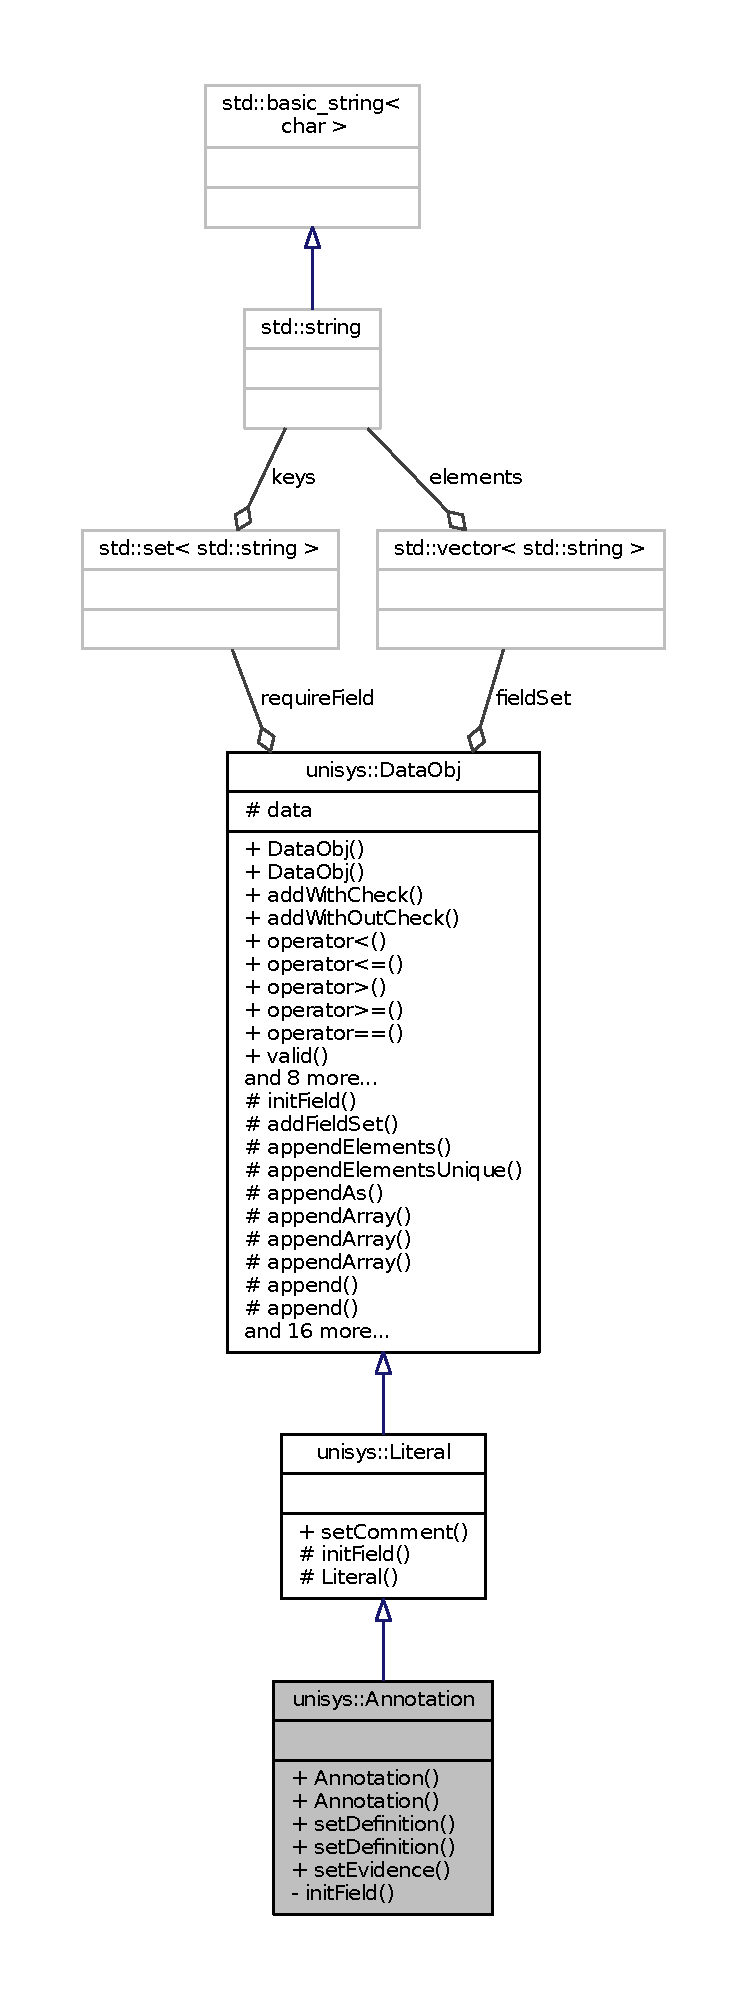
\includegraphics[height=550pt]{classunisys_1_1Annotation__coll__graph}
\end{center}
\end{figure}
\subsection*{Public Member Functions}
\begin{DoxyCompactItemize}
\item 
\hyperlink{classunisys_1_1Annotation_a08702dfa8f734012f7c68d7317a3a540}{Annotation} ()
\begin{DoxyCompactList}\small\item\em Default constructor. \end{DoxyCompactList}\item 
\hyperlink{classunisys_1_1Annotation_a36f2000bdfe49eef240bdf0dabd3df2d}{Annotation} (mongo\-::\-B\-S\-O\-N\-Obj const \&bson\-Obj)
\begin{DoxyCompactList}\small\item\em Overloaded constructor is used when retriving data in boson object from database and tranform to C++ object. \end{DoxyCompactList}\item 
void \hyperlink{classunisys_1_1Annotation_a61390650d258397c76f8482318d58741}{set\-Definition} (\hyperlink{classunisys_1_1OntoIdRef}{Onto\-Id\-Ref} \&onto\-Id\-Ref)
\item 
void \hyperlink{classunisys_1_1Annotation_ac10cd6a0c92eb085de8a7e3ba76a8069}{set\-Definition} (std\-::string const \&onto\-Id)
\item 
void \hyperlink{classunisys_1_1Annotation_a61aed5074b5497728e9ce33eeb3e2b4c}{set\-Evidence} (\hyperlink{classunisys_1_1Evidence}{Evidence} \&evidence)
\end{DoxyCompactItemize}
\subsection*{Private Member Functions}
\begin{DoxyCompactItemize}
\item 
void \hyperlink{classunisys_1_1Annotation_a56a0503bd22b05cae674b8d4df046d9e}{init\-Field} ()
\begin{DoxyCompactList}\small\item\em function for init field in the object \end{DoxyCompactList}\end{DoxyCompactItemize}
\subsection*{Additional Inherited Members}


\subsection{Detailed Description}
The C++ representative class for annotation data class. 

\begin{DoxyVerb}        BSON structure:
        {   
            comment: <string>,
            definition: {$ref: <collname>, $id: <idvalue>}, #format by idref class
            evidence: <EvidenceBSONStructure>
        }\end{DoxyVerb}
 

\subsection{Constructor \& Destructor Documentation}
\hypertarget{classunisys_1_1Annotation_a08702dfa8f734012f7c68d7317a3a540}{\index{unisys\-::\-Annotation@{unisys\-::\-Annotation}!Annotation@{Annotation}}
\index{Annotation@{Annotation}!unisys::Annotation@{unisys\-::\-Annotation}}
\subsubsection[{Annotation}]{\setlength{\rightskip}{0pt plus 5cm}unisys\-::\-Annotation\-::\-Annotation (
\begin{DoxyParamCaption}
{}
\end{DoxyParamCaption}
)}}\label{classunisys_1_1Annotation_a08702dfa8f734012f7c68d7317a3a540}


Default constructor. 

\hypertarget{classunisys_1_1Annotation_a36f2000bdfe49eef240bdf0dabd3df2d}{\index{unisys\-::\-Annotation@{unisys\-::\-Annotation}!Annotation@{Annotation}}
\index{Annotation@{Annotation}!unisys::Annotation@{unisys\-::\-Annotation}}
\subsubsection[{Annotation}]{\setlength{\rightskip}{0pt plus 5cm}unisys\-::\-Annotation\-::\-Annotation (
\begin{DoxyParamCaption}
\item[{mongo\-::\-B\-S\-O\-N\-Obj const \&}]{bson\-Obj}
\end{DoxyParamCaption}
)}}\label{classunisys_1_1Annotation_a36f2000bdfe49eef240bdf0dabd3df2d}


Overloaded constructor is used when retriving data in boson object from database and tranform to C++ object. 



\subsection{Member Function Documentation}
\hypertarget{classunisys_1_1Annotation_a56a0503bd22b05cae674b8d4df046d9e}{\index{unisys\-::\-Annotation@{unisys\-::\-Annotation}!init\-Field@{init\-Field}}
\index{init\-Field@{init\-Field}!unisys::Annotation@{unisys\-::\-Annotation}}
\subsubsection[{init\-Field}]{\setlength{\rightskip}{0pt plus 5cm}void unisys\-::\-Annotation\-::init\-Field (
\begin{DoxyParamCaption}
{}
\end{DoxyParamCaption}
)\hspace{0.3cm}{\ttfamily [private]}, {\ttfamily [virtual]}}}\label{classunisys_1_1Annotation_a56a0503bd22b05cae674b8d4df046d9e}


function for init field in the object 



Reimplemented from \hyperlink{classunisys_1_1Literal_a769b8f41e99619d8635f83d18a02bc1f}{unisys\-::\-Literal}.

\hypertarget{classunisys_1_1Annotation_a61390650d258397c76f8482318d58741}{\index{unisys\-::\-Annotation@{unisys\-::\-Annotation}!set\-Definition@{set\-Definition}}
\index{set\-Definition@{set\-Definition}!unisys::Annotation@{unisys\-::\-Annotation}}
\subsubsection[{set\-Definition}]{\setlength{\rightskip}{0pt plus 5cm}void unisys\-::\-Annotation\-::set\-Definition (
\begin{DoxyParamCaption}
\item[{{\bf Onto\-Id\-Ref} \&}]{onto\-Id\-Ref}
\end{DoxyParamCaption}
)}}\label{classunisys_1_1Annotation_a61390650d258397c76f8482318d58741}
\hypertarget{classunisys_1_1Annotation_ac10cd6a0c92eb085de8a7e3ba76a8069}{\index{unisys\-::\-Annotation@{unisys\-::\-Annotation}!set\-Definition@{set\-Definition}}
\index{set\-Definition@{set\-Definition}!unisys::Annotation@{unisys\-::\-Annotation}}
\subsubsection[{set\-Definition}]{\setlength{\rightskip}{0pt plus 5cm}void unisys\-::\-Annotation\-::set\-Definition (
\begin{DoxyParamCaption}
\item[{std\-::string const \&}]{onto\-Id}
\end{DoxyParamCaption}
)}}\label{classunisys_1_1Annotation_ac10cd6a0c92eb085de8a7e3ba76a8069}
\hypertarget{classunisys_1_1Annotation_a61aed5074b5497728e9ce33eeb3e2b4c}{\index{unisys\-::\-Annotation@{unisys\-::\-Annotation}!set\-Evidence@{set\-Evidence}}
\index{set\-Evidence@{set\-Evidence}!unisys::Annotation@{unisys\-::\-Annotation}}
\subsubsection[{set\-Evidence}]{\setlength{\rightskip}{0pt plus 5cm}void unisys\-::\-Annotation\-::set\-Evidence (
\begin{DoxyParamCaption}
\item[{{\bf Evidence} \&}]{evidence}
\end{DoxyParamCaption}
)}}\label{classunisys_1_1Annotation_a61aed5074b5497728e9ce33eeb3e2b4c}


The documentation for this class was generated from the following file\-:\begin{DoxyCompactItemize}
\item 
\hyperlink{LitClass_8h}{Lit\-Class.\-h}\end{DoxyCompactItemize}

\hypertarget{classunisys_1_1BatchInsert}{\section{unisys\-:\-:Batch\-Insert Class Reference}
\label{classunisys_1_1BatchInsert}\index{unisys\-::\-Batch\-Insert@{unisys\-::\-Batch\-Insert}}
}


{\ttfamily \#include $<$updater.\-h$>$}



Inheritance diagram for unisys\-:\-:Batch\-Insert\-:
\nopagebreak
\begin{figure}[H]
\begin{center}
\leavevmode
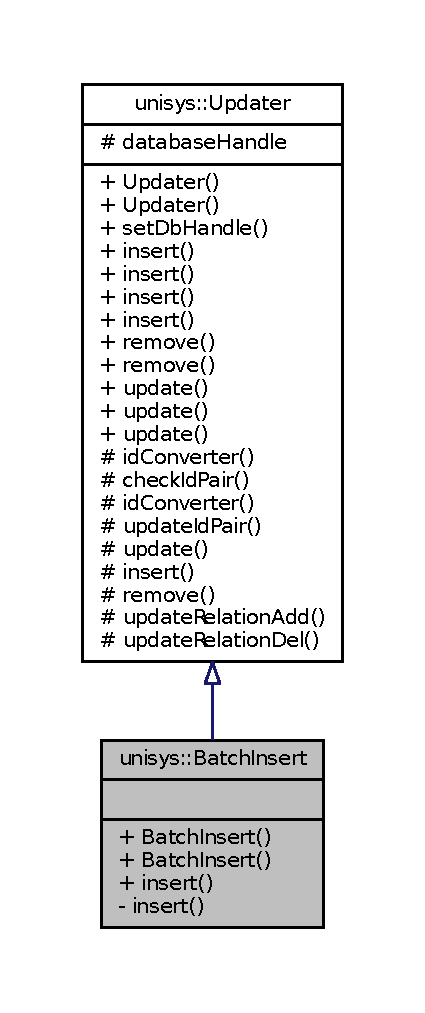
\includegraphics[width=204pt]{classunisys_1_1BatchInsert__inherit__graph}
\end{center}
\end{figure}


Collaboration diagram for unisys\-:\-:Batch\-Insert\-:
\nopagebreak
\begin{figure}[H]
\begin{center}
\leavevmode
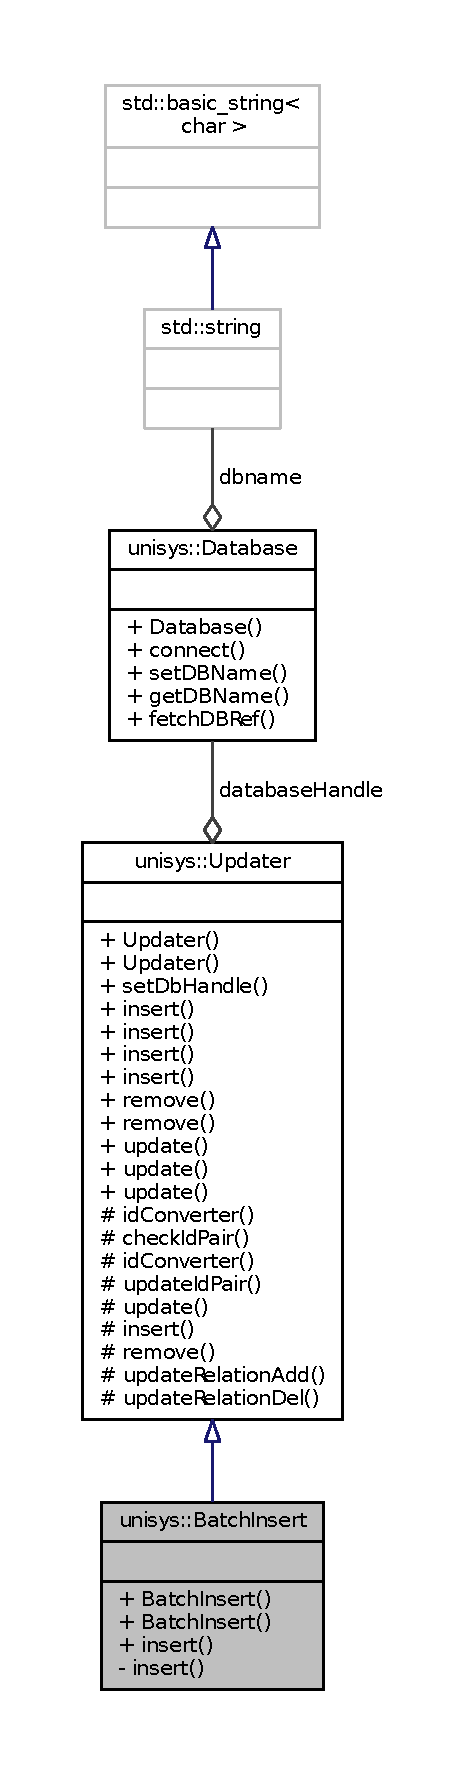
\includegraphics[height=550pt]{classunisys_1_1BatchInsert__coll__graph}
\end{center}
\end{figure}
\subsection*{Public Member Functions}
\begin{DoxyCompactItemize}
\item 
\hyperlink{classunisys_1_1BatchInsert_a6ae2cc7e268f83cf1ecc99058b62011d}{Batch\-Insert} ()
\item 
\hyperlink{classunisys_1_1BatchInsert_a751ec752b94fd29565e5e515a3f83d50}{Batch\-Insert} (\hyperlink{classunisys_1_1Database}{Database} $\ast$database\-Handle\-Pt)
\item 
{\footnotesize template$<$class my\-Type $>$ }\\std\-::vector$<$ mongo\-::\-B\-S\-O\-N\-Obj $>$ \hyperlink{classunisys_1_1BatchInsert_a3fa151c77cd33efbbd97311aa51acbcd}{insert} (std\-::vector$<$ my\-Type $>$ data\-List, std\-::string id\-N\-S=\char`\"{}\char`\"{}, unsigned int start\-Id=0, std\-::string id\-Prefix=\char`\"{}\char`\"{}, unsigned int version=0, bool with\-Ver=true, bool dryrun=false)  throw (\-Update\-Error, Data\-Error)
\end{DoxyCompactItemize}
\subsection*{Private Member Functions}
\begin{DoxyCompactItemize}
\item 
std\-::vector$<$ mongo\-::\-B\-S\-O\-N\-Obj $>$ \hyperlink{classunisys_1_1BatchInsert_adc2dcf20f672d02d3f73dfee371e9c2a}{insert} (std\-::vector$<$ mongo\-::\-B\-S\-O\-N\-Obj $>$ data\-List, std\-::string id\-N\-S=\char`\"{}\char`\"{}, int start\-Id=1, bool dryrun=false)  throw (\-Update\-Error, Data\-Error)
\end{DoxyCompactItemize}
\subsection*{Additional Inherited Members}


\subsection{Constructor \& Destructor Documentation}
\hypertarget{classunisys_1_1BatchInsert_a6ae2cc7e268f83cf1ecc99058b62011d}{\index{unisys\-::\-Batch\-Insert@{unisys\-::\-Batch\-Insert}!Batch\-Insert@{Batch\-Insert}}
\index{Batch\-Insert@{Batch\-Insert}!unisys::BatchInsert@{unisys\-::\-Batch\-Insert}}
\subsubsection[{Batch\-Insert}]{\setlength{\rightskip}{0pt plus 5cm}unisys\-::\-Batch\-Insert\-::\-Batch\-Insert (
\begin{DoxyParamCaption}
{}
\end{DoxyParamCaption}
)}}\label{classunisys_1_1BatchInsert_a6ae2cc7e268f83cf1ecc99058b62011d}
\hypertarget{classunisys_1_1BatchInsert_a751ec752b94fd29565e5e515a3f83d50}{\index{unisys\-::\-Batch\-Insert@{unisys\-::\-Batch\-Insert}!Batch\-Insert@{Batch\-Insert}}
\index{Batch\-Insert@{Batch\-Insert}!unisys::BatchInsert@{unisys\-::\-Batch\-Insert}}
\subsubsection[{Batch\-Insert}]{\setlength{\rightskip}{0pt plus 5cm}unisys\-::\-Batch\-Insert\-::\-Batch\-Insert (
\begin{DoxyParamCaption}
\item[{{\bf Database} $\ast$}]{database\-Handle\-Pt}
\end{DoxyParamCaption}
)}}\label{classunisys_1_1BatchInsert_a751ec752b94fd29565e5e515a3f83d50}


\subsection{Member Function Documentation}
\hypertarget{classunisys_1_1BatchInsert_adc2dcf20f672d02d3f73dfee371e9c2a}{\index{unisys\-::\-Batch\-Insert@{unisys\-::\-Batch\-Insert}!insert@{insert}}
\index{insert@{insert}!unisys::BatchInsert@{unisys\-::\-Batch\-Insert}}
\subsubsection[{insert}]{\setlength{\rightskip}{0pt plus 5cm}std\-::vector$<$mongo\-::\-B\-S\-O\-N\-Obj$>$ unisys\-::\-Batch\-Insert\-::insert (
\begin{DoxyParamCaption}
\item[{std\-::vector$<$ mongo\-::\-B\-S\-O\-N\-Obj $>$}]{data\-List, }
\item[{std\-::string}]{id\-N\-S = {\ttfamily \char`\"{}\char`\"{}}, }
\item[{int}]{start\-Id = {\ttfamily 1}, }
\item[{bool}]{dryrun = {\ttfamily false}}
\end{DoxyParamCaption}
)  throw ({\bf Update\-Error}, {\bf Data\-Error})\hspace{0.3cm}{\ttfamily [private]}}}\label{classunisys_1_1BatchInsert_adc2dcf20f672d02d3f73dfee371e9c2a}
\hypertarget{classunisys_1_1BatchInsert_a3fa151c77cd33efbbd97311aa51acbcd}{\index{unisys\-::\-Batch\-Insert@{unisys\-::\-Batch\-Insert}!insert@{insert}}
\index{insert@{insert}!unisys::BatchInsert@{unisys\-::\-Batch\-Insert}}
\subsubsection[{insert}]{\setlength{\rightskip}{0pt plus 5cm}template$<$class my\-Type $>$ std\-::vector$<$mongo\-::\-B\-S\-O\-N\-Obj$>$ unisys\-::\-Batch\-Insert\-::insert (
\begin{DoxyParamCaption}
\item[{std\-::vector$<$ my\-Type $>$}]{data\-List, }
\item[{std\-::string}]{id\-N\-S = {\ttfamily \char`\"{}\char`\"{}}, }
\item[{unsigned int}]{start\-Id = {\ttfamily 0}, }
\item[{std\-::string}]{id\-Prefix = {\ttfamily \char`\"{}\char`\"{}}, }
\item[{unsigned int}]{version = {\ttfamily 0}, }
\item[{bool}]{with\-Ver = {\ttfamily true}, }
\item[{bool}]{dryrun = {\ttfamily false}}
\end{DoxyParamCaption}
)  throw ({\bf Update\-Error}, {\bf Data\-Error})}}\label{classunisys_1_1BatchInsert_a3fa151c77cd33efbbd97311aa51acbcd}


The documentation for this class was generated from the following file\-:\begin{DoxyCompactItemize}
\item 
\hyperlink{updater_8h}{updater.\-h}\end{DoxyCompactItemize}

\hypertarget{classunisys_1_1BiochemicalReaction}{\section{unisys\-:\-:Biochemical\-Reaction Class Reference}
\label{classunisys_1_1BiochemicalReaction}\index{unisys\-::\-Biochemical\-Reaction@{unisys\-::\-Biochemical\-Reaction}}
}


This class is for miriam cross reference annotation.  




{\ttfamily \#include $<$Obj\-Class.\-h$>$}



Inheritance diagram for unisys\-:\-:Biochemical\-Reaction\-:
\nopagebreak
\begin{figure}[H]
\begin{center}
\leavevmode
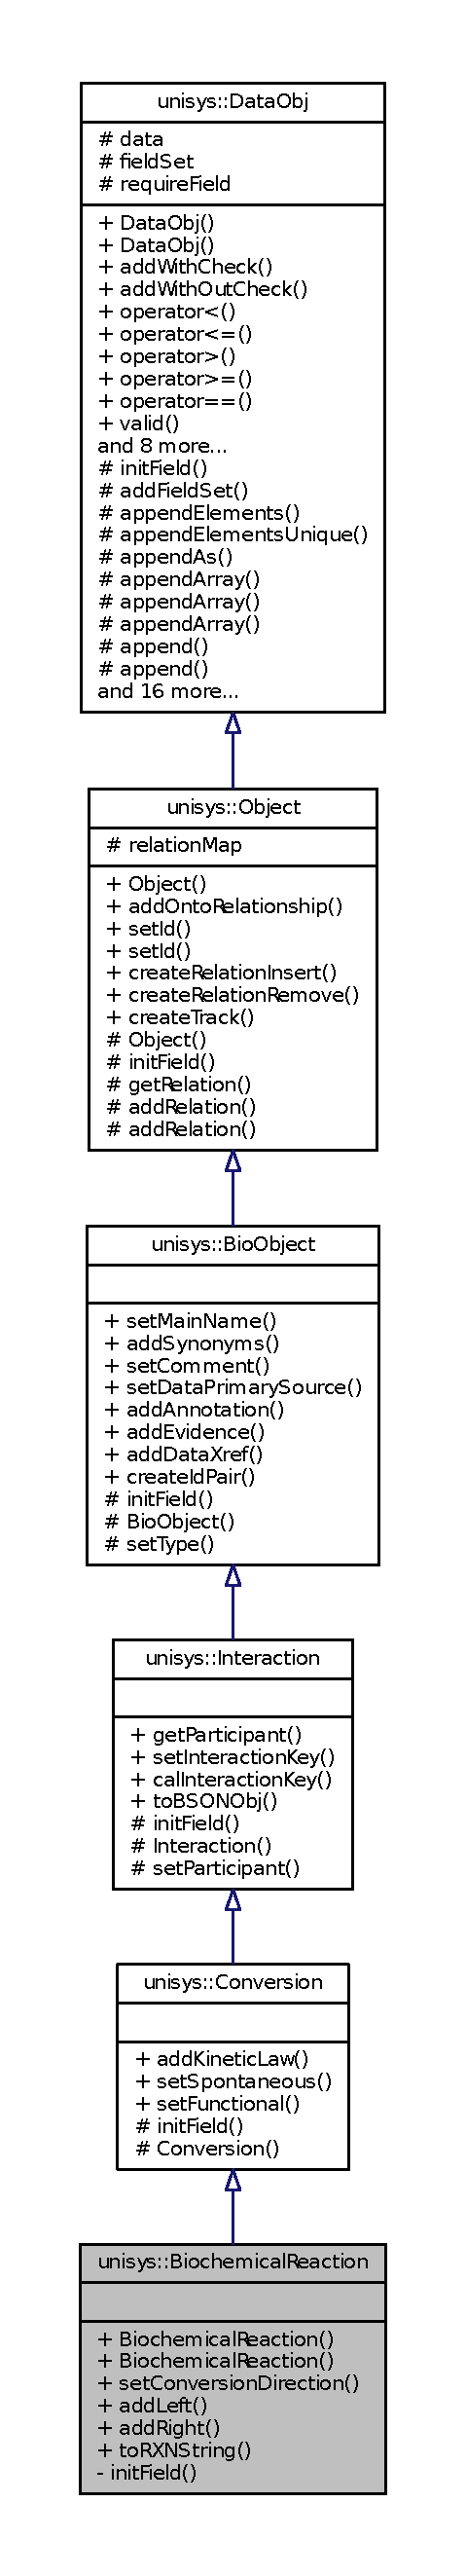
\includegraphics[height=550pt]{classunisys_1_1BiochemicalReaction__inherit__graph}
\end{center}
\end{figure}


Collaboration diagram for unisys\-:\-:Biochemical\-Reaction\-:
\nopagebreak
\begin{figure}[H]
\begin{center}
\leavevmode
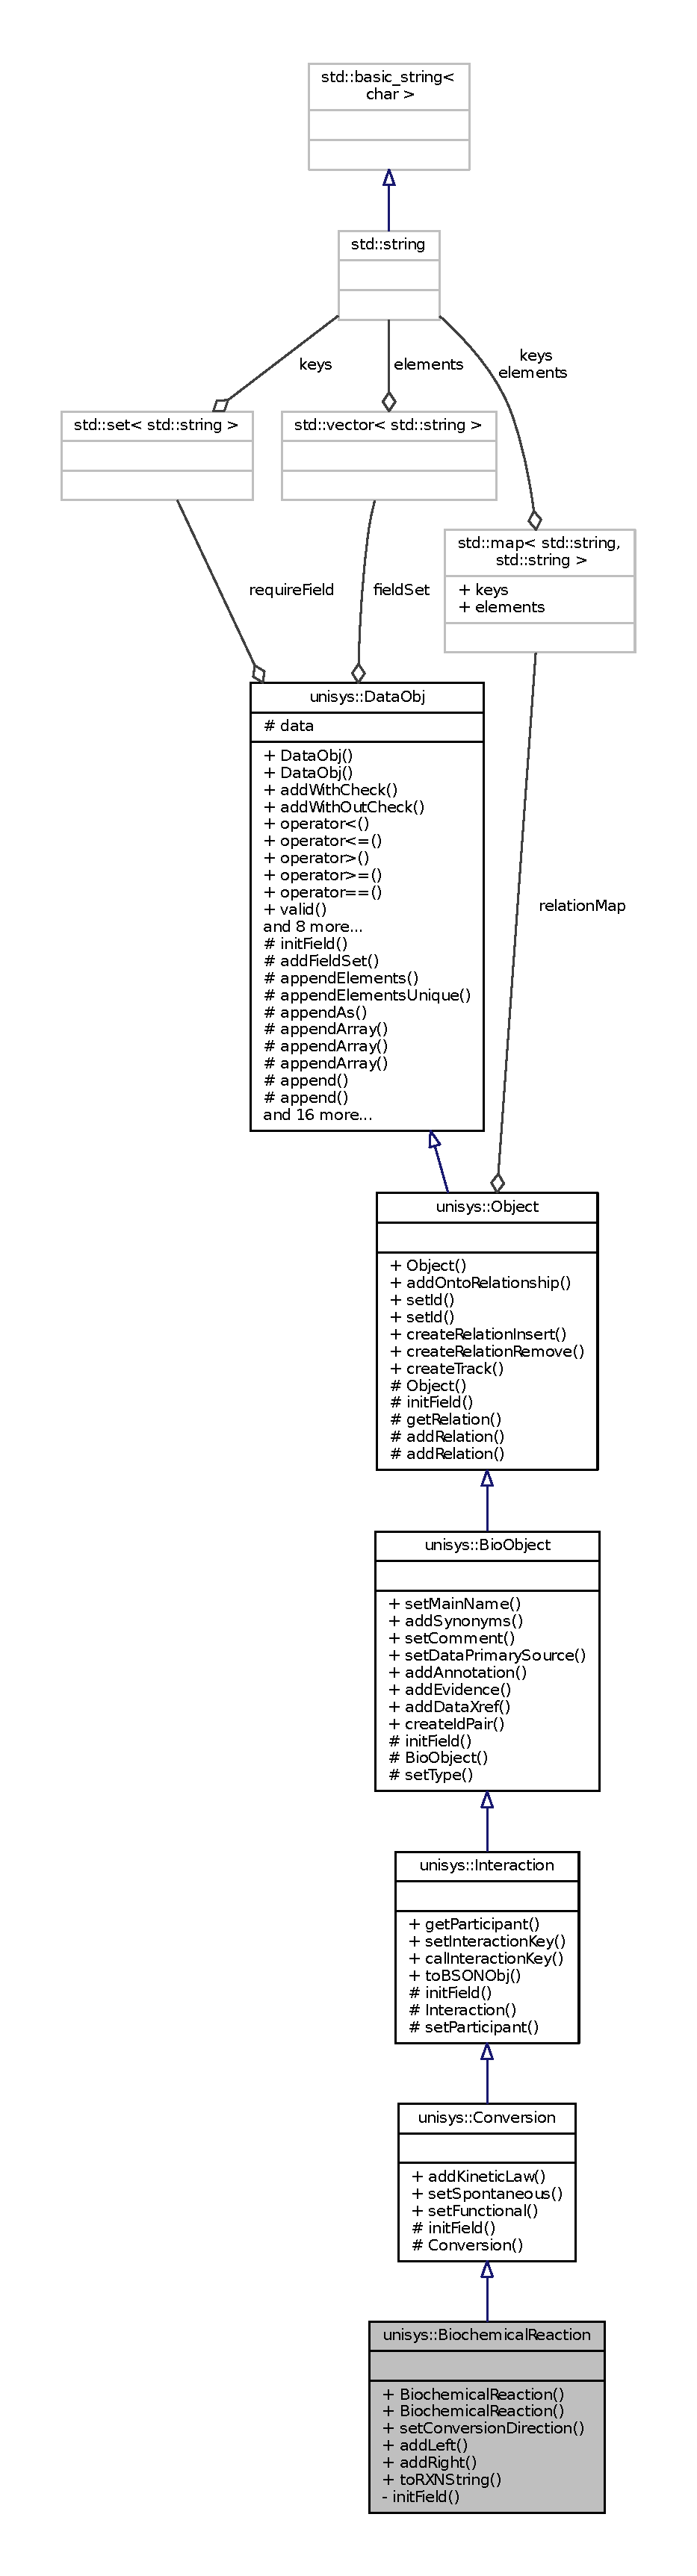
\includegraphics[height=550pt]{classunisys_1_1BiochemicalReaction__coll__graph}
\end{center}
\end{figure}
\subsection*{Public Member Functions}
\begin{DoxyCompactItemize}
\item 
\hyperlink{classunisys_1_1BiochemicalReaction_a1058034c07346ef992ba78c3260b1ac6}{Biochemical\-Reaction} ()
\begin{DoxyCompactList}\small\item\em Default constructor. \end{DoxyCompactList}\item 
\hyperlink{classunisys_1_1BiochemicalReaction_a50d32f8995cb279b41c37a731f48bfe1}{Biochemical\-Reaction} (mongo\-::\-B\-S\-O\-N\-Obj const \&bson\-Obj)
\begin{DoxyCompactList}\small\item\em Overloaded constructor is used when retriving data in boson object from database and tranform to C++ object. \end{DoxyCompactList}\item 
void \hyperlink{classunisys_1_1BiochemicalReaction_a33073d1e349bdcb5cf5c95fda55e2ede}{set\-Conversion\-Direction} (std\-::string const \&direction=\char`\"{}=\char`\"{})
\item 
void \hyperlink{classunisys_1_1BiochemicalReaction_a5f80d7411cbfa867c583d8137d9c4db5}{add\-Left} (\hyperlink{classunisys_1_1PEIdRef}{P\-E\-Id\-Ref} \&pe\-Id\-Ref, double coefficient)
\begin{DoxyCompactList}\small\item\em Add left participants of reaction. \end{DoxyCompactList}\item 
void \hyperlink{classunisys_1_1BiochemicalReaction_a62c77e5e197b9a89c7d2d3a9555ff14d}{add\-Right} (\hyperlink{classunisys_1_1PEIdRef}{P\-E\-Id\-Ref} \&pe\-Id\-Ref, double coefficient)
\begin{DoxyCompactList}\small\item\em Add right participants of reaction. \end{DoxyCompactList}\item 
std\-::string \hyperlink{classunisys_1_1BiochemicalReaction_ac0ae394fe6271ab66a88ec8fe36a68ae}{to\-R\-X\-N\-String} (std\-::string const \&compartment) const 
\end{DoxyCompactItemize}
\subsection*{Private Member Functions}
\begin{DoxyCompactItemize}
\item 
void \hyperlink{classunisys_1_1BiochemicalReaction_a61d5cb519be2ac672ae8e243abdc7489}{init\-Field} ()
\end{DoxyCompactItemize}
\subsection*{Additional Inherited Members}


\subsection{Detailed Description}
This class is for miriam cross reference annotation. 

\begin{DoxyVerb}        BSON structure:
        {   
            _id: <string>, #madatory
            type: <string>,
            ontologyRelationship: {<RelationshipBOSON>, <RelationshipBOSON>, ...},
            name: {<string>,<string>, ...}
            comment: <string>,
            dataPrimarySource: <XrefBOSON>,
            functionAnnotation: {<AnnotationBOSON>, <AnnotationBOSON>, ...},
            evidence: {<EvidenceBOSON>, <EvidenceBOSON>, ...},
            dataxref: {<XrefBOSON>, <XrefBOSON>, ...},
            relation: {<StoichiometryBOSON>, <StoichiometryBOSON>, ...},
            interactionKey: <string>,
            conversionDirection: <DbRef>,
            kineticLaw: {<MathMLBOSON>, <MathMLBOSON>, ...}
            spontaneous: <string>,
            functional: <string>
        }\end{DoxyVerb}
 

\subsection{Constructor \& Destructor Documentation}
\hypertarget{classunisys_1_1BiochemicalReaction_a1058034c07346ef992ba78c3260b1ac6}{\index{unisys\-::\-Biochemical\-Reaction@{unisys\-::\-Biochemical\-Reaction}!Biochemical\-Reaction@{Biochemical\-Reaction}}
\index{Biochemical\-Reaction@{Biochemical\-Reaction}!unisys::BiochemicalReaction@{unisys\-::\-Biochemical\-Reaction}}
\subsubsection[{Biochemical\-Reaction}]{\setlength{\rightskip}{0pt plus 5cm}unisys\-::\-Biochemical\-Reaction\-::\-Biochemical\-Reaction (
\begin{DoxyParamCaption}
{}
\end{DoxyParamCaption}
)}}\label{classunisys_1_1BiochemicalReaction_a1058034c07346ef992ba78c3260b1ac6}


Default constructor. 

\hypertarget{classunisys_1_1BiochemicalReaction_a50d32f8995cb279b41c37a731f48bfe1}{\index{unisys\-::\-Biochemical\-Reaction@{unisys\-::\-Biochemical\-Reaction}!Biochemical\-Reaction@{Biochemical\-Reaction}}
\index{Biochemical\-Reaction@{Biochemical\-Reaction}!unisys::BiochemicalReaction@{unisys\-::\-Biochemical\-Reaction}}
\subsubsection[{Biochemical\-Reaction}]{\setlength{\rightskip}{0pt plus 5cm}unisys\-::\-Biochemical\-Reaction\-::\-Biochemical\-Reaction (
\begin{DoxyParamCaption}
\item[{mongo\-::\-B\-S\-O\-N\-Obj const \&}]{bson\-Obj}
\end{DoxyParamCaption}
)}}\label{classunisys_1_1BiochemicalReaction_a50d32f8995cb279b41c37a731f48bfe1}


Overloaded constructor is used when retriving data in boson object from database and tranform to C++ object. 



\subsection{Member Function Documentation}
\hypertarget{classunisys_1_1BiochemicalReaction_a5f80d7411cbfa867c583d8137d9c4db5}{\index{unisys\-::\-Biochemical\-Reaction@{unisys\-::\-Biochemical\-Reaction}!add\-Left@{add\-Left}}
\index{add\-Left@{add\-Left}!unisys::BiochemicalReaction@{unisys\-::\-Biochemical\-Reaction}}
\subsubsection[{add\-Left}]{\setlength{\rightskip}{0pt plus 5cm}void unisys\-::\-Biochemical\-Reaction\-::add\-Left (
\begin{DoxyParamCaption}
\item[{{\bf P\-E\-Id\-Ref} \&}]{pe\-Id\-Ref, }
\item[{double}]{coefficient}
\end{DoxyParamCaption}
)}}\label{classunisys_1_1BiochemicalReaction_a5f80d7411cbfa867c583d8137d9c4db5}


Add left participants of reaction. 

\hypertarget{classunisys_1_1BiochemicalReaction_a62c77e5e197b9a89c7d2d3a9555ff14d}{\index{unisys\-::\-Biochemical\-Reaction@{unisys\-::\-Biochemical\-Reaction}!add\-Right@{add\-Right}}
\index{add\-Right@{add\-Right}!unisys::BiochemicalReaction@{unisys\-::\-Biochemical\-Reaction}}
\subsubsection[{add\-Right}]{\setlength{\rightskip}{0pt plus 5cm}void unisys\-::\-Biochemical\-Reaction\-::add\-Right (
\begin{DoxyParamCaption}
\item[{{\bf P\-E\-Id\-Ref} \&}]{pe\-Id\-Ref, }
\item[{double}]{coefficient}
\end{DoxyParamCaption}
)}}\label{classunisys_1_1BiochemicalReaction_a62c77e5e197b9a89c7d2d3a9555ff14d}


Add right participants of reaction. 

\hypertarget{classunisys_1_1BiochemicalReaction_a61d5cb519be2ac672ae8e243abdc7489}{\index{unisys\-::\-Biochemical\-Reaction@{unisys\-::\-Biochemical\-Reaction}!init\-Field@{init\-Field}}
\index{init\-Field@{init\-Field}!unisys::BiochemicalReaction@{unisys\-::\-Biochemical\-Reaction}}
\subsubsection[{init\-Field}]{\setlength{\rightskip}{0pt plus 5cm}void unisys\-::\-Biochemical\-Reaction\-::init\-Field (
\begin{DoxyParamCaption}
{}
\end{DoxyParamCaption}
)\hspace{0.3cm}{\ttfamily [private]}, {\ttfamily [virtual]}}}\label{classunisys_1_1BiochemicalReaction_a61d5cb519be2ac672ae8e243abdc7489}


Reimplemented from \hyperlink{classunisys_1_1Conversion_adafab2a857d6b15d5e07a0d59f4f6596}{unisys\-::\-Conversion}.

\hypertarget{classunisys_1_1BiochemicalReaction_a33073d1e349bdcb5cf5c95fda55e2ede}{\index{unisys\-::\-Biochemical\-Reaction@{unisys\-::\-Biochemical\-Reaction}!set\-Conversion\-Direction@{set\-Conversion\-Direction}}
\index{set\-Conversion\-Direction@{set\-Conversion\-Direction}!unisys::BiochemicalReaction@{unisys\-::\-Biochemical\-Reaction}}
\subsubsection[{set\-Conversion\-Direction}]{\setlength{\rightskip}{0pt plus 5cm}void unisys\-::\-Biochemical\-Reaction\-::set\-Conversion\-Direction (
\begin{DoxyParamCaption}
\item[{std\-::string const \&}]{direction = {\ttfamily \char`\"{}=\char`\"{}}}
\end{DoxyParamCaption}
)}}\label{classunisys_1_1BiochemicalReaction_a33073d1e349bdcb5cf5c95fda55e2ede}
\hypertarget{classunisys_1_1BiochemicalReaction_ac0ae394fe6271ab66a88ec8fe36a68ae}{\index{unisys\-::\-Biochemical\-Reaction@{unisys\-::\-Biochemical\-Reaction}!to\-R\-X\-N\-String@{to\-R\-X\-N\-String}}
\index{to\-R\-X\-N\-String@{to\-R\-X\-N\-String}!unisys::BiochemicalReaction@{unisys\-::\-Biochemical\-Reaction}}
\subsubsection[{to\-R\-X\-N\-String}]{\setlength{\rightskip}{0pt plus 5cm}std\-::string unisys\-::\-Biochemical\-Reaction\-::to\-R\-X\-N\-String (
\begin{DoxyParamCaption}
\item[{std\-::string const \&}]{compartment}
\end{DoxyParamCaption}
) const}}\label{classunisys_1_1BiochemicalReaction_ac0ae394fe6271ab66a88ec8fe36a68ae}


The documentation for this class was generated from the following file\-:\begin{DoxyCompactItemize}
\item 
\hyperlink{ObjClass_8h}{Obj\-Class.\-h}\end{DoxyCompactItemize}

\hypertarget{classunisys_1_1BiochemicalReactionWithTransport}{\section{unisys\-:\-:Biochemical\-Reaction\-With\-Transport Class Reference}
\label{classunisys_1_1BiochemicalReactionWithTransport}\index{unisys\-::\-Biochemical\-Reaction\-With\-Transport@{unisys\-::\-Biochemical\-Reaction\-With\-Transport}}
}


This class is for miriam cross reference annotation.  




{\ttfamily \#include $<$Obj\-Class.\-h$>$}



Inheritance diagram for unisys\-:\-:Biochemical\-Reaction\-With\-Transport\-:
\nopagebreak
\begin{figure}[H]
\begin{center}
\leavevmode
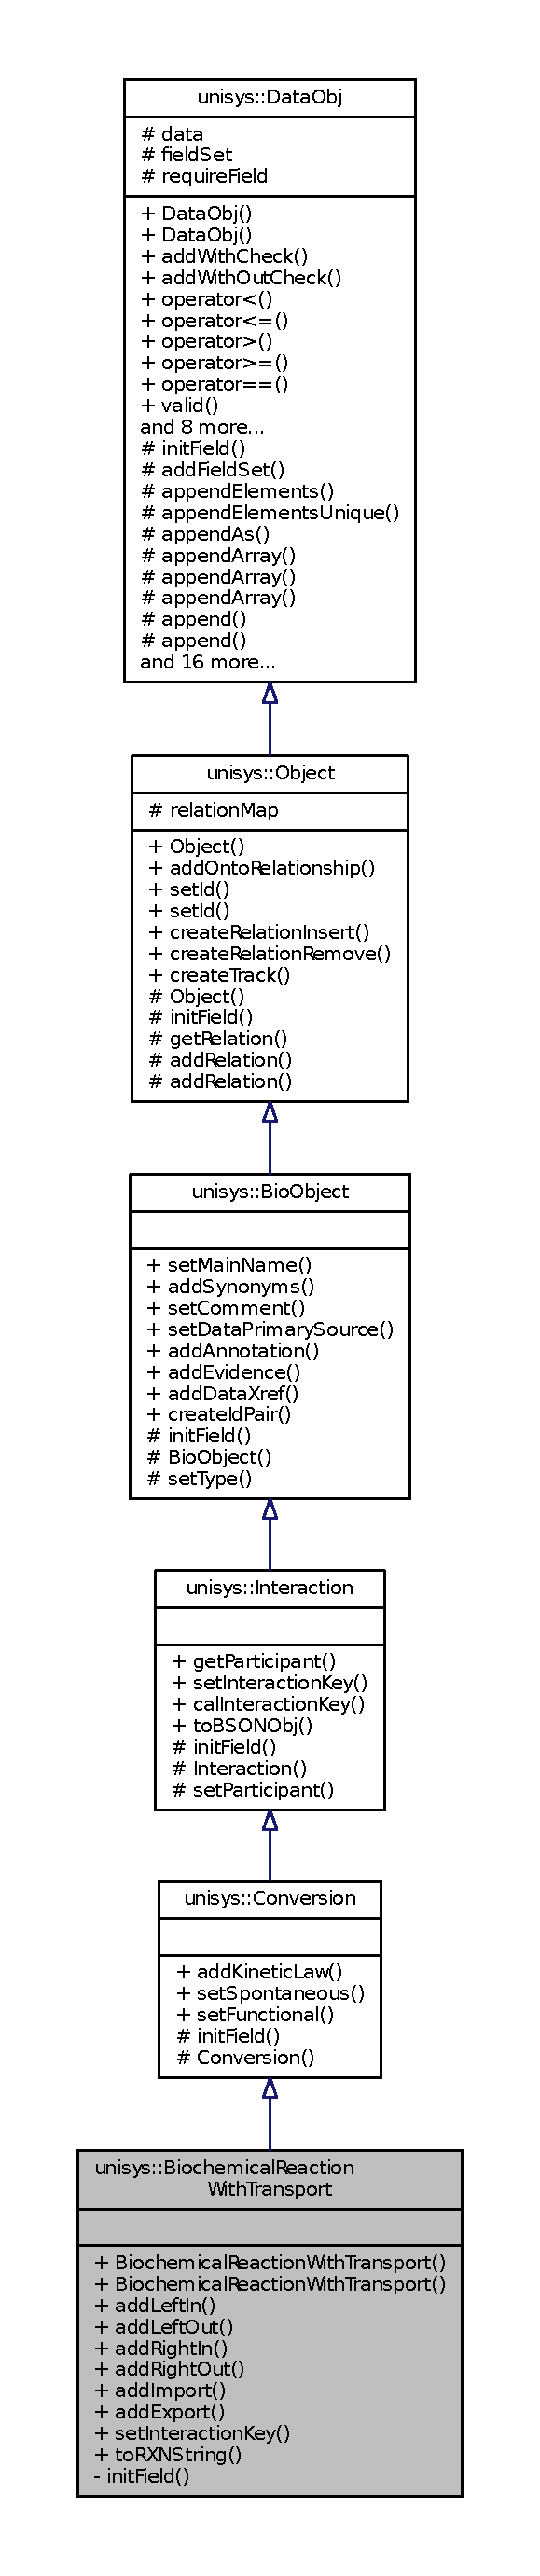
\includegraphics[height=550pt]{classunisys_1_1BiochemicalReactionWithTransport__inherit__graph}
\end{center}
\end{figure}


Collaboration diagram for unisys\-:\-:Biochemical\-Reaction\-With\-Transport\-:
\nopagebreak
\begin{figure}[H]
\begin{center}
\leavevmode
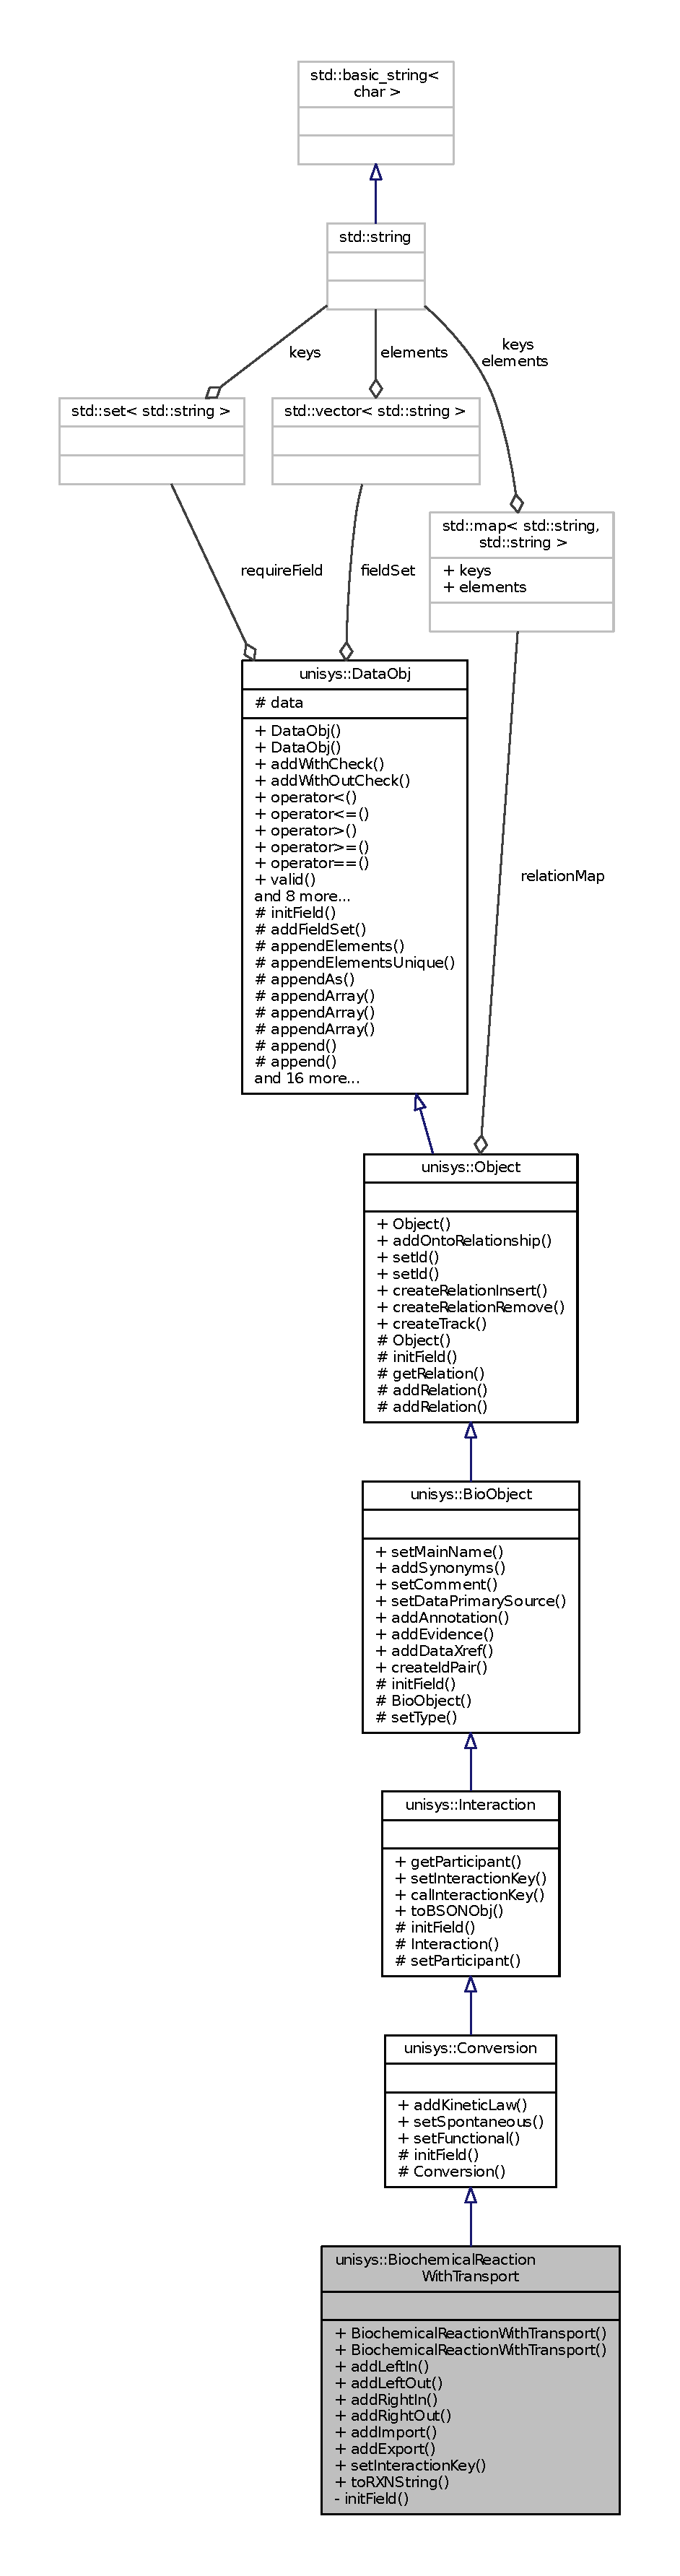
\includegraphics[height=550pt]{classunisys_1_1BiochemicalReactionWithTransport__coll__graph}
\end{center}
\end{figure}
\subsection*{Public Member Functions}
\begin{DoxyCompactItemize}
\item 
\hyperlink{classunisys_1_1BiochemicalReactionWithTransport_a0123a9057d275ac2a5c1c7ece8760c45}{Biochemical\-Reaction\-With\-Transport} ()
\begin{DoxyCompactList}\small\item\em Default constructor. \end{DoxyCompactList}\item 
\hyperlink{classunisys_1_1BiochemicalReactionWithTransport_ae43f3ef0de1f8adcc07c3a0aae37ce5d}{Biochemical\-Reaction\-With\-Transport} (mongo\-::\-B\-S\-O\-N\-Obj const \&bson\-Obj)
\begin{DoxyCompactList}\small\item\em Overloaded constructor is used when retriving data in boson object from database and tranform to C++ object. \end{DoxyCompactList}\item 
void \hyperlink{classunisys_1_1BiochemicalReactionWithTransport_a1a2cf84dd0f2ff964c30d128672fe6f4}{add\-Left\-In} (\hyperlink{classunisys_1_1PEIdRef}{P\-E\-Id\-Ref} \&pe\-Id\-Ref, double coefficient)
\item 
void \hyperlink{classunisys_1_1BiochemicalReactionWithTransport_ae19e6120575e8cf5bcc79f83024d8f75}{add\-Left\-Out} (\hyperlink{classunisys_1_1PEIdRef}{P\-E\-Id\-Ref} \&pe\-Id\-Ref, double coefficient)
\item 
void \hyperlink{classunisys_1_1BiochemicalReactionWithTransport_a61aeefa2111c40134c9072c96fb84627}{add\-Right\-In} (\hyperlink{classunisys_1_1PEIdRef}{P\-E\-Id\-Ref} \&pe\-Id\-Ref, double coefficient)
\item 
void \hyperlink{classunisys_1_1BiochemicalReactionWithTransport_a3567d77df0d2f9ebc7b5c14bcfcfa2c2}{add\-Right\-Out} (\hyperlink{classunisys_1_1PEIdRef}{P\-E\-Id\-Ref} \&pe\-Id\-Ref, double coefficient)
\item 
void \hyperlink{classunisys_1_1BiochemicalReactionWithTransport_adf0e10be1ddb1bc58591a8e305d4bfd7}{add\-Import} (\hyperlink{classunisys_1_1PEIdRef}{P\-E\-Id\-Ref} \&pe\-Id\-Ref, double coefficient)
\item 
void \hyperlink{classunisys_1_1BiochemicalReactionWithTransport_a95ad769f30ccf98bde213af8e282c979}{add\-Export} (\hyperlink{classunisys_1_1PEIdRef}{P\-E\-Id\-Ref} \&pe\-Id\-Ref, double coefficient)
\item 
void \hyperlink{classunisys_1_1BiochemicalReactionWithTransport_aa47aa306b9157473a48ad8e83a27cda3}{set\-Interaction\-Key} ()
\item 
std\-::string \hyperlink{classunisys_1_1BiochemicalReactionWithTransport_af0a913d23fbc37e845840570249b46f4}{to\-R\-X\-N\-String} (std\-::string const \&outside, std\-::string const \&inside) const 
\begin{DoxyCompactList}\small\item\em converse to a string of reaction \end{DoxyCompactList}\end{DoxyCompactItemize}
\subsection*{Private Member Functions}
\begin{DoxyCompactItemize}
\item 
void \hyperlink{classunisys_1_1BiochemicalReactionWithTransport_a9999c6a5353e9b62056691cf0187f04f}{init\-Field} ()
\end{DoxyCompactItemize}
\subsection*{Additional Inherited Members}


\subsection{Detailed Description}
This class is for miriam cross reference annotation. 

\begin{DoxyVerb}        BSON structure:
        {   
            _id: <string>, #madatory
            type: <string>,
            ontologyRelationship: {<RelationshipBOSON>, <RelationshipBOSON>, ...},
            name: {<string>,<string>, ...}
            comment: <string>,
            dataPrimarySource: <XrefBOSON>,
            functionAnnotation: {<AnnotationBOSON>, <AnnotationBOSON>, ...},
            evidence: {<EvidenceBOSON>, <EvidenceBOSON>, ...},
            dataxref: {<XrefBOSON>, <XrefBOSON>, ...},
            participant: {<StoichiometryBOSON>, <StoichiometryBOSON>, ...},
            interactionKey: <string>,
            conversionDirection: <DbRef>,
            kineticLaw: {<MathMLBOSON>, <MathMLBOSON>, ...}
            spontaneous: <string>,
            functional: <string>
        }\end{DoxyVerb}
 

\subsection{Constructor \& Destructor Documentation}
\hypertarget{classunisys_1_1BiochemicalReactionWithTransport_a0123a9057d275ac2a5c1c7ece8760c45}{\index{unisys\-::\-Biochemical\-Reaction\-With\-Transport@{unisys\-::\-Biochemical\-Reaction\-With\-Transport}!Biochemical\-Reaction\-With\-Transport@{Biochemical\-Reaction\-With\-Transport}}
\index{Biochemical\-Reaction\-With\-Transport@{Biochemical\-Reaction\-With\-Transport}!unisys::BiochemicalReactionWithTransport@{unisys\-::\-Biochemical\-Reaction\-With\-Transport}}
\subsubsection[{Biochemical\-Reaction\-With\-Transport}]{\setlength{\rightskip}{0pt plus 5cm}unisys\-::\-Biochemical\-Reaction\-With\-Transport\-::\-Biochemical\-Reaction\-With\-Transport (
\begin{DoxyParamCaption}
{}
\end{DoxyParamCaption}
)}}\label{classunisys_1_1BiochemicalReactionWithTransport_a0123a9057d275ac2a5c1c7ece8760c45}


Default constructor. 

\hypertarget{classunisys_1_1BiochemicalReactionWithTransport_ae43f3ef0de1f8adcc07c3a0aae37ce5d}{\index{unisys\-::\-Biochemical\-Reaction\-With\-Transport@{unisys\-::\-Biochemical\-Reaction\-With\-Transport}!Biochemical\-Reaction\-With\-Transport@{Biochemical\-Reaction\-With\-Transport}}
\index{Biochemical\-Reaction\-With\-Transport@{Biochemical\-Reaction\-With\-Transport}!unisys::BiochemicalReactionWithTransport@{unisys\-::\-Biochemical\-Reaction\-With\-Transport}}
\subsubsection[{Biochemical\-Reaction\-With\-Transport}]{\setlength{\rightskip}{0pt plus 5cm}unisys\-::\-Biochemical\-Reaction\-With\-Transport\-::\-Biochemical\-Reaction\-With\-Transport (
\begin{DoxyParamCaption}
\item[{mongo\-::\-B\-S\-O\-N\-Obj const \&}]{bson\-Obj}
\end{DoxyParamCaption}
)}}\label{classunisys_1_1BiochemicalReactionWithTransport_ae43f3ef0de1f8adcc07c3a0aae37ce5d}


Overloaded constructor is used when retriving data in boson object from database and tranform to C++ object. 



\subsection{Member Function Documentation}
\hypertarget{classunisys_1_1BiochemicalReactionWithTransport_a95ad769f30ccf98bde213af8e282c979}{\index{unisys\-::\-Biochemical\-Reaction\-With\-Transport@{unisys\-::\-Biochemical\-Reaction\-With\-Transport}!add\-Export@{add\-Export}}
\index{add\-Export@{add\-Export}!unisys::BiochemicalReactionWithTransport@{unisys\-::\-Biochemical\-Reaction\-With\-Transport}}
\subsubsection[{add\-Export}]{\setlength{\rightskip}{0pt plus 5cm}void unisys\-::\-Biochemical\-Reaction\-With\-Transport\-::add\-Export (
\begin{DoxyParamCaption}
\item[{{\bf P\-E\-Id\-Ref} \&}]{pe\-Id\-Ref, }
\item[{double}]{coefficient}
\end{DoxyParamCaption}
)}}\label{classunisys_1_1BiochemicalReactionWithTransport_a95ad769f30ccf98bde213af8e282c979}
\hypertarget{classunisys_1_1BiochemicalReactionWithTransport_adf0e10be1ddb1bc58591a8e305d4bfd7}{\index{unisys\-::\-Biochemical\-Reaction\-With\-Transport@{unisys\-::\-Biochemical\-Reaction\-With\-Transport}!add\-Import@{add\-Import}}
\index{add\-Import@{add\-Import}!unisys::BiochemicalReactionWithTransport@{unisys\-::\-Biochemical\-Reaction\-With\-Transport}}
\subsubsection[{add\-Import}]{\setlength{\rightskip}{0pt plus 5cm}void unisys\-::\-Biochemical\-Reaction\-With\-Transport\-::add\-Import (
\begin{DoxyParamCaption}
\item[{{\bf P\-E\-Id\-Ref} \&}]{pe\-Id\-Ref, }
\item[{double}]{coefficient}
\end{DoxyParamCaption}
)}}\label{classunisys_1_1BiochemicalReactionWithTransport_adf0e10be1ddb1bc58591a8e305d4bfd7}
\hypertarget{classunisys_1_1BiochemicalReactionWithTransport_a1a2cf84dd0f2ff964c30d128672fe6f4}{\index{unisys\-::\-Biochemical\-Reaction\-With\-Transport@{unisys\-::\-Biochemical\-Reaction\-With\-Transport}!add\-Left\-In@{add\-Left\-In}}
\index{add\-Left\-In@{add\-Left\-In}!unisys::BiochemicalReactionWithTransport@{unisys\-::\-Biochemical\-Reaction\-With\-Transport}}
\subsubsection[{add\-Left\-In}]{\setlength{\rightskip}{0pt plus 5cm}void unisys\-::\-Biochemical\-Reaction\-With\-Transport\-::add\-Left\-In (
\begin{DoxyParamCaption}
\item[{{\bf P\-E\-Id\-Ref} \&}]{pe\-Id\-Ref, }
\item[{double}]{coefficient}
\end{DoxyParamCaption}
)}}\label{classunisys_1_1BiochemicalReactionWithTransport_a1a2cf84dd0f2ff964c30d128672fe6f4}
\hypertarget{classunisys_1_1BiochemicalReactionWithTransport_ae19e6120575e8cf5bcc79f83024d8f75}{\index{unisys\-::\-Biochemical\-Reaction\-With\-Transport@{unisys\-::\-Biochemical\-Reaction\-With\-Transport}!add\-Left\-Out@{add\-Left\-Out}}
\index{add\-Left\-Out@{add\-Left\-Out}!unisys::BiochemicalReactionWithTransport@{unisys\-::\-Biochemical\-Reaction\-With\-Transport}}
\subsubsection[{add\-Left\-Out}]{\setlength{\rightskip}{0pt plus 5cm}void unisys\-::\-Biochemical\-Reaction\-With\-Transport\-::add\-Left\-Out (
\begin{DoxyParamCaption}
\item[{{\bf P\-E\-Id\-Ref} \&}]{pe\-Id\-Ref, }
\item[{double}]{coefficient}
\end{DoxyParamCaption}
)}}\label{classunisys_1_1BiochemicalReactionWithTransport_ae19e6120575e8cf5bcc79f83024d8f75}
\hypertarget{classunisys_1_1BiochemicalReactionWithTransport_a61aeefa2111c40134c9072c96fb84627}{\index{unisys\-::\-Biochemical\-Reaction\-With\-Transport@{unisys\-::\-Biochemical\-Reaction\-With\-Transport}!add\-Right\-In@{add\-Right\-In}}
\index{add\-Right\-In@{add\-Right\-In}!unisys::BiochemicalReactionWithTransport@{unisys\-::\-Biochemical\-Reaction\-With\-Transport}}
\subsubsection[{add\-Right\-In}]{\setlength{\rightskip}{0pt plus 5cm}void unisys\-::\-Biochemical\-Reaction\-With\-Transport\-::add\-Right\-In (
\begin{DoxyParamCaption}
\item[{{\bf P\-E\-Id\-Ref} \&}]{pe\-Id\-Ref, }
\item[{double}]{coefficient}
\end{DoxyParamCaption}
)}}\label{classunisys_1_1BiochemicalReactionWithTransport_a61aeefa2111c40134c9072c96fb84627}
\hypertarget{classunisys_1_1BiochemicalReactionWithTransport_a3567d77df0d2f9ebc7b5c14bcfcfa2c2}{\index{unisys\-::\-Biochemical\-Reaction\-With\-Transport@{unisys\-::\-Biochemical\-Reaction\-With\-Transport}!add\-Right\-Out@{add\-Right\-Out}}
\index{add\-Right\-Out@{add\-Right\-Out}!unisys::BiochemicalReactionWithTransport@{unisys\-::\-Biochemical\-Reaction\-With\-Transport}}
\subsubsection[{add\-Right\-Out}]{\setlength{\rightskip}{0pt plus 5cm}void unisys\-::\-Biochemical\-Reaction\-With\-Transport\-::add\-Right\-Out (
\begin{DoxyParamCaption}
\item[{{\bf P\-E\-Id\-Ref} \&}]{pe\-Id\-Ref, }
\item[{double}]{coefficient}
\end{DoxyParamCaption}
)}}\label{classunisys_1_1BiochemicalReactionWithTransport_a3567d77df0d2f9ebc7b5c14bcfcfa2c2}
\hypertarget{classunisys_1_1BiochemicalReactionWithTransport_a9999c6a5353e9b62056691cf0187f04f}{\index{unisys\-::\-Biochemical\-Reaction\-With\-Transport@{unisys\-::\-Biochemical\-Reaction\-With\-Transport}!init\-Field@{init\-Field}}
\index{init\-Field@{init\-Field}!unisys::BiochemicalReactionWithTransport@{unisys\-::\-Biochemical\-Reaction\-With\-Transport}}
\subsubsection[{init\-Field}]{\setlength{\rightskip}{0pt plus 5cm}void unisys\-::\-Biochemical\-Reaction\-With\-Transport\-::init\-Field (
\begin{DoxyParamCaption}
{}
\end{DoxyParamCaption}
)\hspace{0.3cm}{\ttfamily [private]}, {\ttfamily [virtual]}}}\label{classunisys_1_1BiochemicalReactionWithTransport_a9999c6a5353e9b62056691cf0187f04f}


Reimplemented from \hyperlink{classunisys_1_1Conversion_adafab2a857d6b15d5e07a0d59f4f6596}{unisys\-::\-Conversion}.

\hypertarget{classunisys_1_1BiochemicalReactionWithTransport_aa47aa306b9157473a48ad8e83a27cda3}{\index{unisys\-::\-Biochemical\-Reaction\-With\-Transport@{unisys\-::\-Biochemical\-Reaction\-With\-Transport}!set\-Interaction\-Key@{set\-Interaction\-Key}}
\index{set\-Interaction\-Key@{set\-Interaction\-Key}!unisys::BiochemicalReactionWithTransport@{unisys\-::\-Biochemical\-Reaction\-With\-Transport}}
\subsubsection[{set\-Interaction\-Key}]{\setlength{\rightskip}{0pt plus 5cm}void unisys\-::\-Biochemical\-Reaction\-With\-Transport\-::set\-Interaction\-Key (
\begin{DoxyParamCaption}
{}
\end{DoxyParamCaption}
)}}\label{classunisys_1_1BiochemicalReactionWithTransport_aa47aa306b9157473a48ad8e83a27cda3}


Reimplemented from \hyperlink{classunisys_1_1Interaction_a73354f785c9c853654a58b2c1a2339ea}{unisys\-::\-Interaction}.

\hypertarget{classunisys_1_1BiochemicalReactionWithTransport_af0a913d23fbc37e845840570249b46f4}{\index{unisys\-::\-Biochemical\-Reaction\-With\-Transport@{unisys\-::\-Biochemical\-Reaction\-With\-Transport}!to\-R\-X\-N\-String@{to\-R\-X\-N\-String}}
\index{to\-R\-X\-N\-String@{to\-R\-X\-N\-String}!unisys::BiochemicalReactionWithTransport@{unisys\-::\-Biochemical\-Reaction\-With\-Transport}}
\subsubsection[{to\-R\-X\-N\-String}]{\setlength{\rightskip}{0pt plus 5cm}std\-::string unisys\-::\-Biochemical\-Reaction\-With\-Transport\-::to\-R\-X\-N\-String (
\begin{DoxyParamCaption}
\item[{std\-::string const \&}]{outside, }
\item[{std\-::string const \&}]{inside}
\end{DoxyParamCaption}
) const}}\label{classunisys_1_1BiochemicalReactionWithTransport_af0a913d23fbc37e845840570249b46f4}


converse to a string of reaction 


\begin{DoxyParams}{Parameters}
{\em outside} & \\
\hline
{\em inside} & \\
\hline
\end{DoxyParams}


The documentation for this class was generated from the following file\-:\begin{DoxyCompactItemize}
\item 
\hyperlink{ObjClass_8h}{Obj\-Class.\-h}\end{DoxyCompactItemize}

\hypertarget{classunisys_1_1BioObject}{\section{unisys\-:\-:Bio\-Object Class Reference}
\label{classunisys_1_1BioObject}\index{unisys\-::\-Bio\-Object@{unisys\-::\-Bio\-Object}}
}


This class is for miriam cross reference annotation.  




{\ttfamily \#include $<$Obj\-Class.\-h$>$}



Inheritance diagram for unisys\-:\-:Bio\-Object\-:
\nopagebreak
\begin{figure}[H]
\begin{center}
\leavevmode
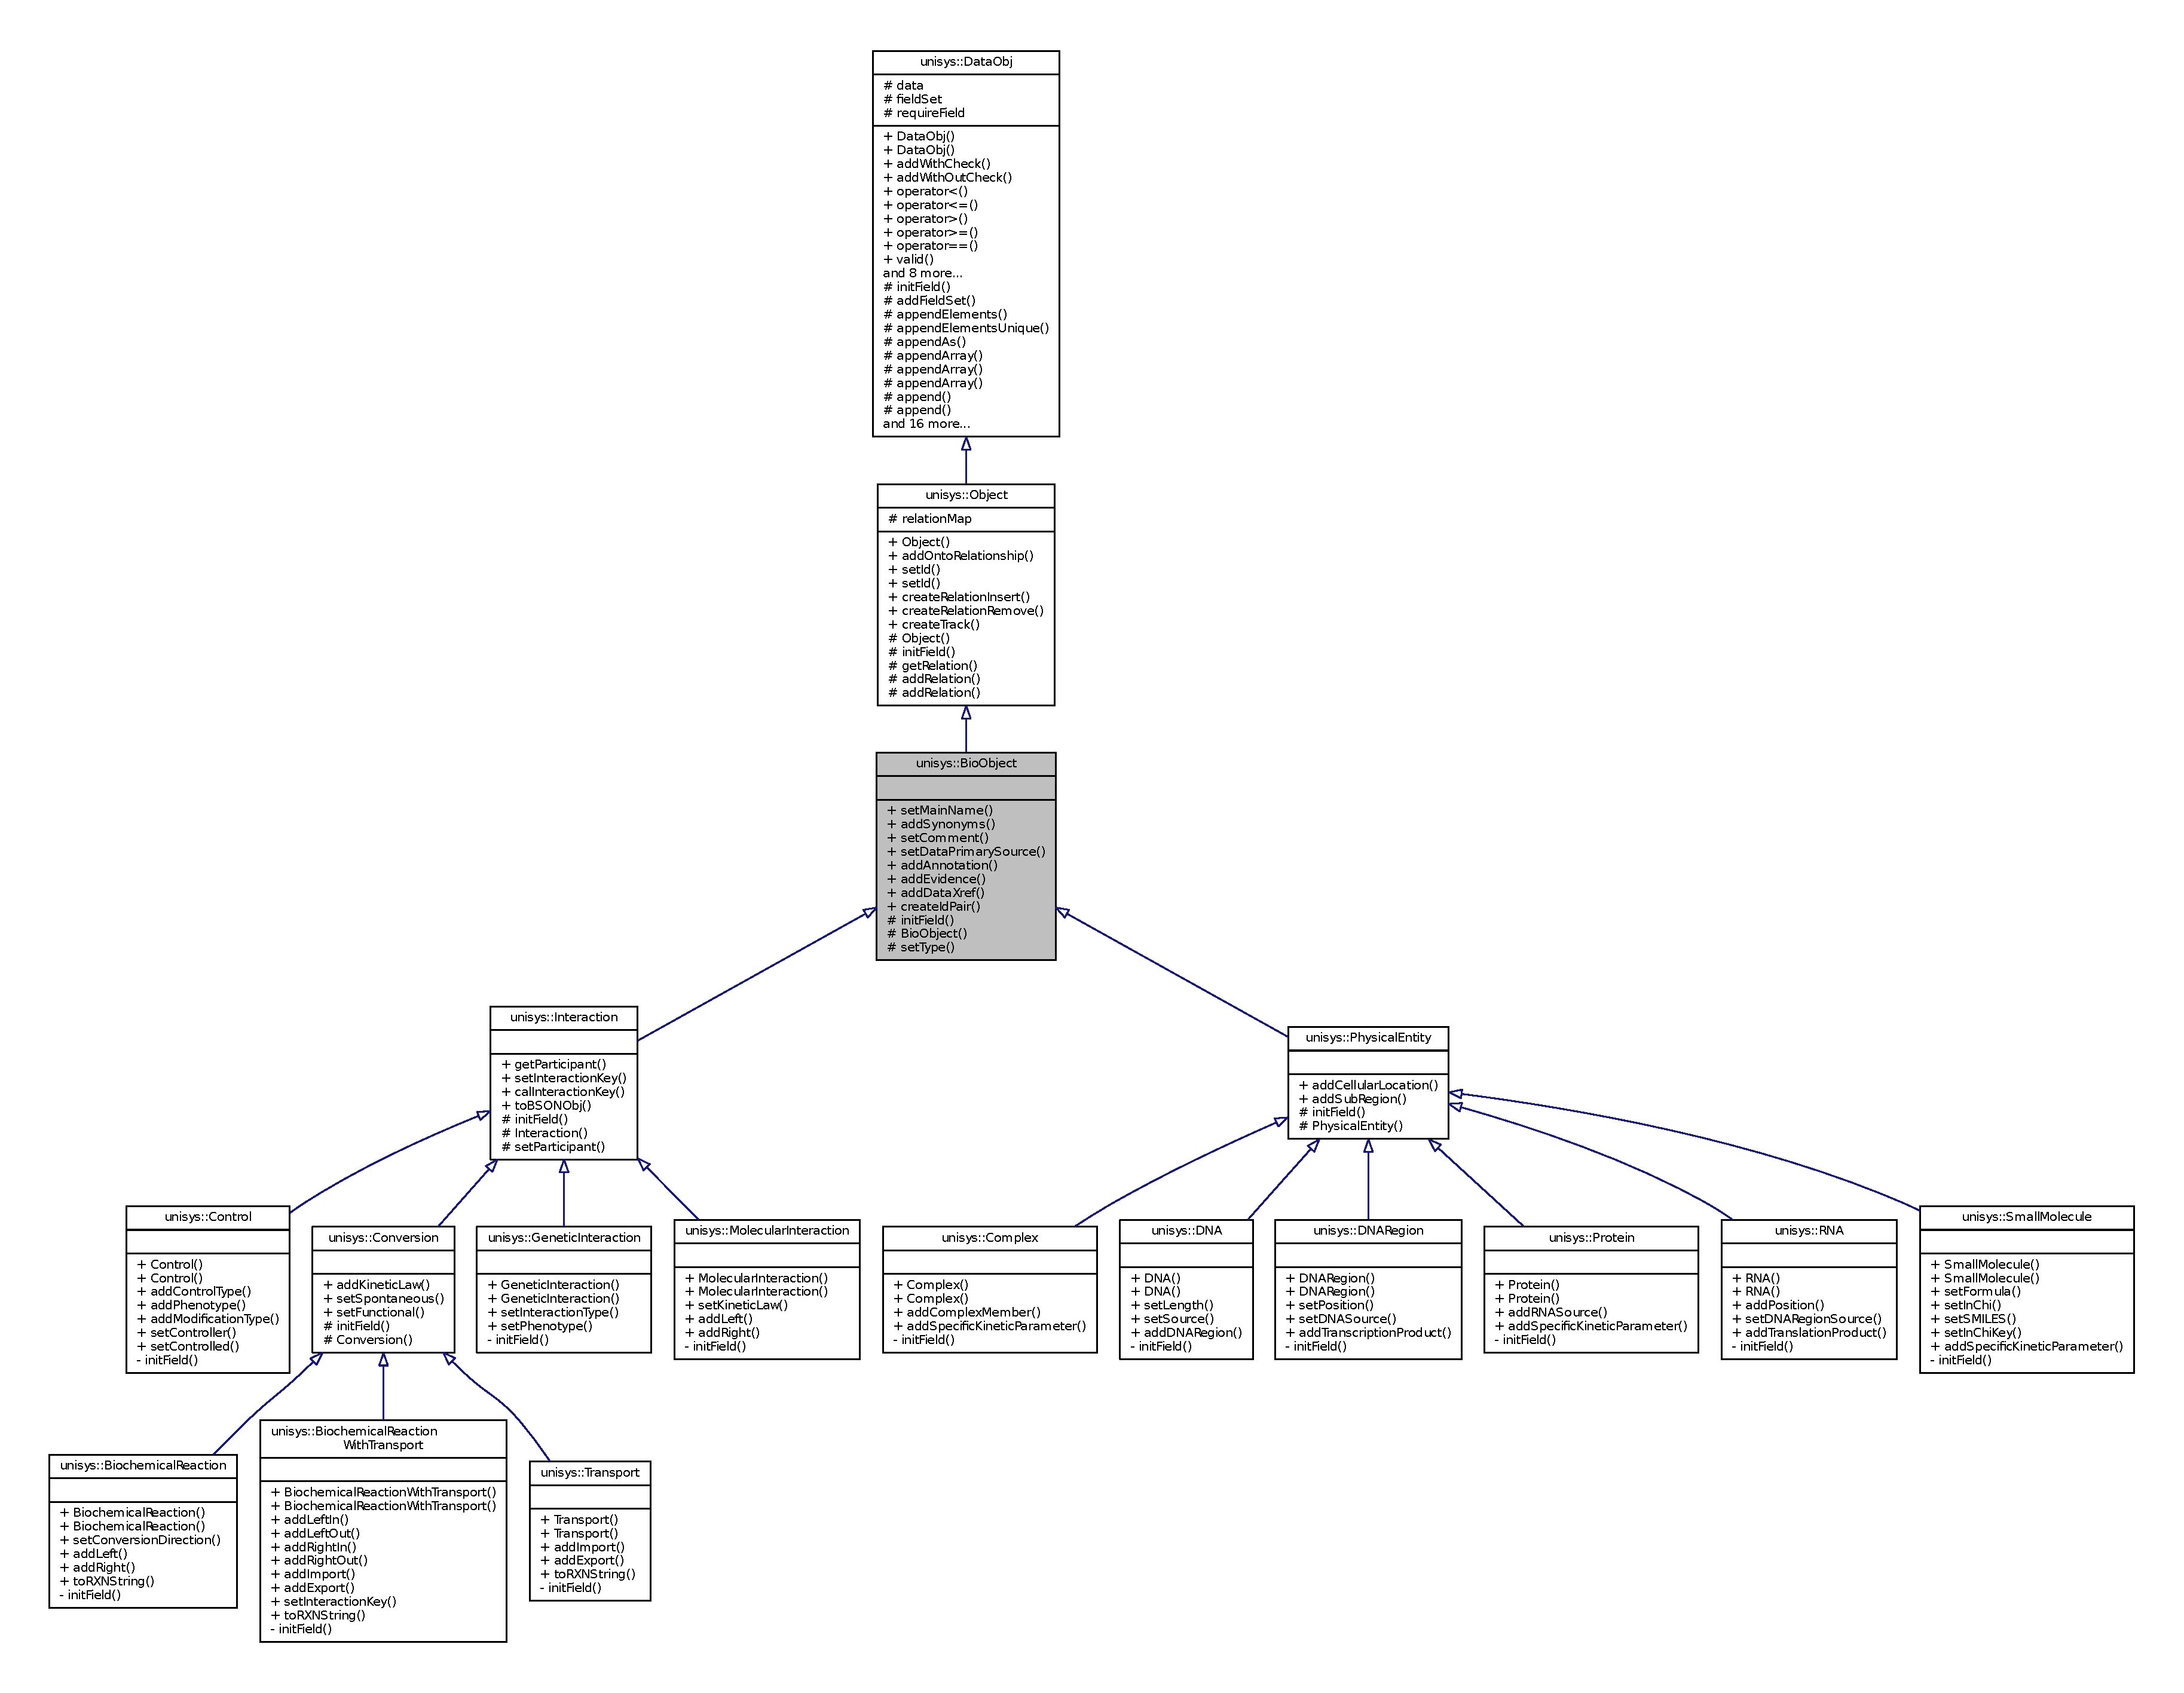
\includegraphics[width=350pt]{classunisys_1_1BioObject__inherit__graph}
\end{center}
\end{figure}


Collaboration diagram for unisys\-:\-:Bio\-Object\-:
\nopagebreak
\begin{figure}[H]
\begin{center}
\leavevmode
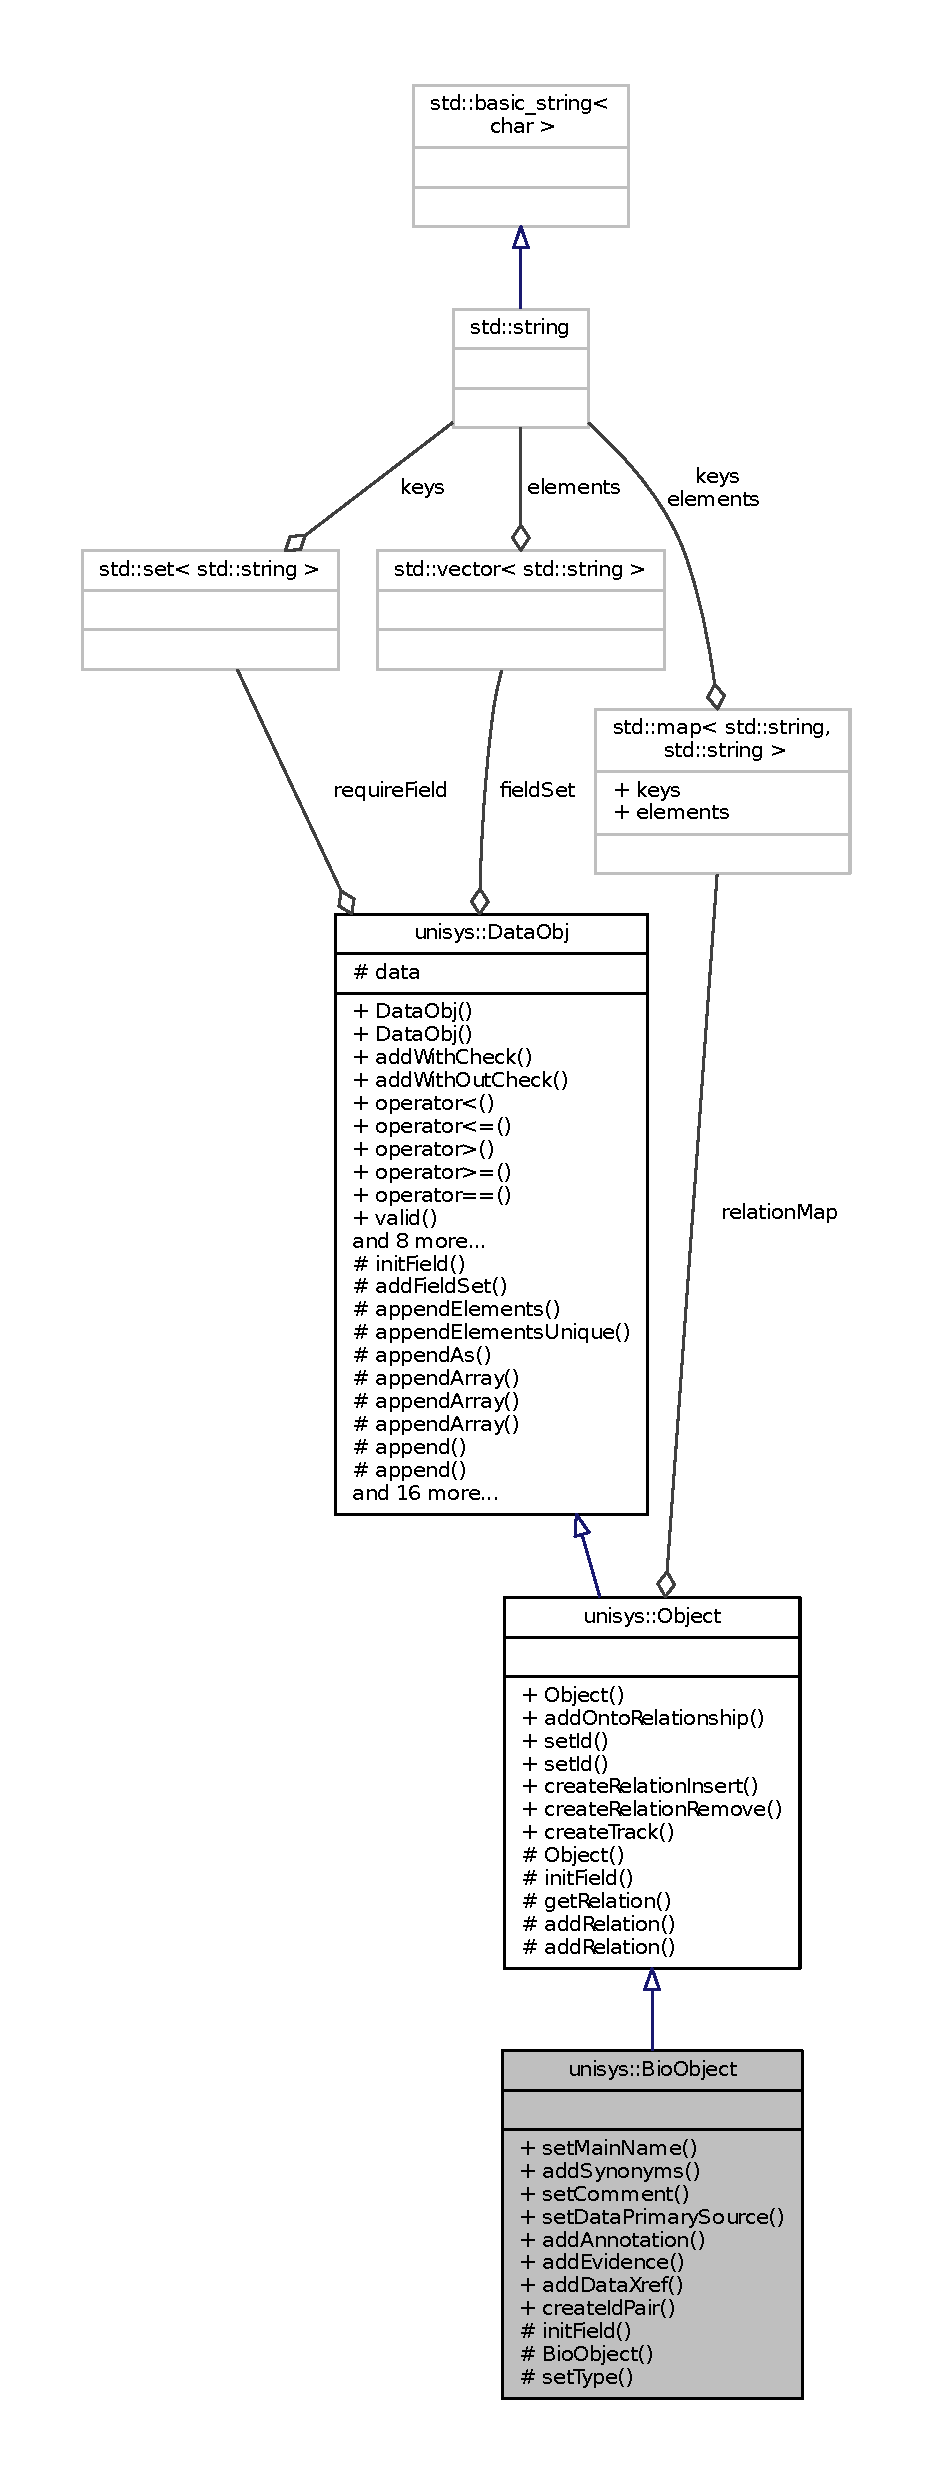
\includegraphics[height=550pt]{classunisys_1_1BioObject__coll__graph}
\end{center}
\end{figure}
\subsection*{Public Member Functions}
\begin{DoxyCompactItemize}
\item 
void \hyperlink{classunisys_1_1BioObject_a97dbae52f1ae5e365ab0730c0562bdd5}{set\-Main\-Name} (std\-::string const \&name)
\item 
void \hyperlink{classunisys_1_1BioObject_a7acdd2ca1ecc7198626bc26966cfb060}{add\-Synonyms} (std\-::string const \&name, std\-::string const \&sep\-\_\-char=\char`\"{},\char`\"{})
\item 
void \hyperlink{classunisys_1_1BioObject_a4db890a15669daff7c5a4f69d524c4c1}{set\-Comment} (std\-::string const \&comment)
\item 
void \hyperlink{classunisys_1_1BioObject_a19ffdccbd63e7611da241cf4b2dac7db}{set\-Data\-Primary\-Source} (\hyperlink{classunisys_1_1Xref}{Xref} xref)
\item 
void \hyperlink{classunisys_1_1BioObject_a99510c967c71bb6c4ef8fa8399262563}{add\-Annotation} (\hyperlink{classunisys_1_1Annotation}{Annotation} \&annotation)
\item 
void \hyperlink{classunisys_1_1BioObject_a3b8e3f3b2cba8e545cb9ccdb45463078}{add\-Evidence} (\hyperlink{classunisys_1_1Evidence}{Evidence} \&evidence)
\item 
void \hyperlink{classunisys_1_1BioObject_a6016ee533dbd19f792ce1091e16865e6}{add\-Data\-Xref} (\hyperlink{classunisys_1_1Xref}{Xref} xref)
\item 
mongo\-::\-B\-S\-O\-N\-Obj \hyperlink{classunisys_1_1BioObject_a44d129aa979ef8a2d27b3afe1046f8af}{create\-Id\-Pair} (bool strict=true) const 
\end{DoxyCompactItemize}
\subsection*{Protected Member Functions}
\begin{DoxyCompactItemize}
\item 
void \hyperlink{classunisys_1_1BioObject_a0437fcc7976ff9e8dc5ce77246c06f71}{init\-Field} ()
\item 
\hyperlink{classunisys_1_1BioObject_a098ee2517786f5d909380771c94ae306}{Bio\-Object} ()
\item 
void \hyperlink{classunisys_1_1BioObject_a24d6362f074cf378024338c636744528}{set\-Type} (std\-::string const \&name)
\end{DoxyCompactItemize}
\subsection*{Additional Inherited Members}


\subsection{Detailed Description}
This class is for miriam cross reference annotation. 

\begin{DoxyVerb}        BSON structure:
        {   
            _id: <string>, #madatory
            ontologyRelationship: {<RelationshipBOSON>, <RelationshipBOSON>, ...},
            name: {<string>,<string>, ...}
            type: <string>, # pathway, collection, chemicalentity, dna, dnaregion, rna, protien, complex, control, molecularinteraction,
                genenticinteraction, biochemicalreaction, transport and reactiontransport
            comment: <string>,
            dataPrimarySource: <XrefBOSON>,
            functionAnnotation: {<AnnotationBOSON>, <AnnotationBOSON>, ...},
            evidence: {<EvidenceBOSON>, <EvidenceBOSON>, ...},
            dataXref: {<XrefBOSON>, <XrefBOSON>, ...}
        }\end{DoxyVerb}
 

\subsection{Constructor \& Destructor Documentation}
\hypertarget{classunisys_1_1BioObject_a098ee2517786f5d909380771c94ae306}{\index{unisys\-::\-Bio\-Object@{unisys\-::\-Bio\-Object}!Bio\-Object@{Bio\-Object}}
\index{Bio\-Object@{Bio\-Object}!unisys::BioObject@{unisys\-::\-Bio\-Object}}
\subsubsection[{Bio\-Object}]{\setlength{\rightskip}{0pt plus 5cm}unisys\-::\-Bio\-Object\-::\-Bio\-Object (
\begin{DoxyParamCaption}
{}
\end{DoxyParamCaption}
)\hspace{0.3cm}{\ttfamily [protected]}}}\label{classunisys_1_1BioObject_a098ee2517786f5d909380771c94ae306}


\subsection{Member Function Documentation}
\hypertarget{classunisys_1_1BioObject_a99510c967c71bb6c4ef8fa8399262563}{\index{unisys\-::\-Bio\-Object@{unisys\-::\-Bio\-Object}!add\-Annotation@{add\-Annotation}}
\index{add\-Annotation@{add\-Annotation}!unisys::BioObject@{unisys\-::\-Bio\-Object}}
\subsubsection[{add\-Annotation}]{\setlength{\rightskip}{0pt plus 5cm}void unisys\-::\-Bio\-Object\-::add\-Annotation (
\begin{DoxyParamCaption}
\item[{{\bf Annotation} \&}]{annotation}
\end{DoxyParamCaption}
)}}\label{classunisys_1_1BioObject_a99510c967c71bb6c4ef8fa8399262563}
\hypertarget{classunisys_1_1BioObject_a6016ee533dbd19f792ce1091e16865e6}{\index{unisys\-::\-Bio\-Object@{unisys\-::\-Bio\-Object}!add\-Data\-Xref@{add\-Data\-Xref}}
\index{add\-Data\-Xref@{add\-Data\-Xref}!unisys::BioObject@{unisys\-::\-Bio\-Object}}
\subsubsection[{add\-Data\-Xref}]{\setlength{\rightskip}{0pt plus 5cm}void unisys\-::\-Bio\-Object\-::add\-Data\-Xref (
\begin{DoxyParamCaption}
\item[{{\bf Xref}}]{xref}
\end{DoxyParamCaption}
)}}\label{classunisys_1_1BioObject_a6016ee533dbd19f792ce1091e16865e6}
\hypertarget{classunisys_1_1BioObject_a3b8e3f3b2cba8e545cb9ccdb45463078}{\index{unisys\-::\-Bio\-Object@{unisys\-::\-Bio\-Object}!add\-Evidence@{add\-Evidence}}
\index{add\-Evidence@{add\-Evidence}!unisys::BioObject@{unisys\-::\-Bio\-Object}}
\subsubsection[{add\-Evidence}]{\setlength{\rightskip}{0pt plus 5cm}void unisys\-::\-Bio\-Object\-::add\-Evidence (
\begin{DoxyParamCaption}
\item[{{\bf Evidence} \&}]{evidence}
\end{DoxyParamCaption}
)}}\label{classunisys_1_1BioObject_a3b8e3f3b2cba8e545cb9ccdb45463078}
\hypertarget{classunisys_1_1BioObject_a7acdd2ca1ecc7198626bc26966cfb060}{\index{unisys\-::\-Bio\-Object@{unisys\-::\-Bio\-Object}!add\-Synonyms@{add\-Synonyms}}
\index{add\-Synonyms@{add\-Synonyms}!unisys::BioObject@{unisys\-::\-Bio\-Object}}
\subsubsection[{add\-Synonyms}]{\setlength{\rightskip}{0pt plus 5cm}void unisys\-::\-Bio\-Object\-::add\-Synonyms (
\begin{DoxyParamCaption}
\item[{std\-::string const \&}]{name, }
\item[{std\-::string const \&}]{sep\-\_\-char = {\ttfamily \char`\"{},\char`\"{}}}
\end{DoxyParamCaption}
)}}\label{classunisys_1_1BioObject_a7acdd2ca1ecc7198626bc26966cfb060}
\hypertarget{classunisys_1_1BioObject_a44d129aa979ef8a2d27b3afe1046f8af}{\index{unisys\-::\-Bio\-Object@{unisys\-::\-Bio\-Object}!create\-Id\-Pair@{create\-Id\-Pair}}
\index{create\-Id\-Pair@{create\-Id\-Pair}!unisys::BioObject@{unisys\-::\-Bio\-Object}}
\subsubsection[{create\-Id\-Pair}]{\setlength{\rightskip}{0pt plus 5cm}mongo\-::\-B\-S\-O\-N\-Obj unisys\-::\-Bio\-Object\-::create\-Id\-Pair (
\begin{DoxyParamCaption}
\item[{bool}]{strict = {\ttfamily true}}
\end{DoxyParamCaption}
) const}}\label{classunisys_1_1BioObject_a44d129aa979ef8a2d27b3afe1046f8af}
\hypertarget{classunisys_1_1BioObject_a0437fcc7976ff9e8dc5ce77246c06f71}{\index{unisys\-::\-Bio\-Object@{unisys\-::\-Bio\-Object}!init\-Field@{init\-Field}}
\index{init\-Field@{init\-Field}!unisys::BioObject@{unisys\-::\-Bio\-Object}}
\subsubsection[{init\-Field}]{\setlength{\rightskip}{0pt plus 5cm}void unisys\-::\-Bio\-Object\-::init\-Field (
\begin{DoxyParamCaption}
{}
\end{DoxyParamCaption}
)\hspace{0.3cm}{\ttfamily [protected]}, {\ttfamily [virtual]}}}\label{classunisys_1_1BioObject_a0437fcc7976ff9e8dc5ce77246c06f71}


Reimplemented from \hyperlink{classunisys_1_1Object_ad0a4afaf978d2cca8a6a27506f06138c}{unisys\-::\-Object}.



Reimplemented in \hyperlink{classunisys_1_1BiochemicalReactionWithTransport_a9999c6a5353e9b62056691cf0187f04f}{unisys\-::\-Biochemical\-Reaction\-With\-Transport}, \hyperlink{classunisys_1_1Transport_a04f17e27ff568c45688cde1a95265dea}{unisys\-::\-Transport}, \hyperlink{classunisys_1_1BiochemicalReaction_a61d5cb519be2ac672ae8e243abdc7489}{unisys\-::\-Biochemical\-Reaction}, \hyperlink{classunisys_1_1Conversion_adafab2a857d6b15d5e07a0d59f4f6596}{unisys\-::\-Conversion}, \hyperlink{classunisys_1_1GeneticInteraction_a946b8270db467290f49a050bd29f55d2}{unisys\-::\-Genetic\-Interaction}, \hyperlink{classunisys_1_1MolecularInteraction_a6bae8353e2734eae8345228f7895665e}{unisys\-::\-Molecular\-Interaction}, \hyperlink{classunisys_1_1Control_ab5bd5022b73b81e3fd18af06027213b1}{unisys\-::\-Control}, \hyperlink{classunisys_1_1Interaction_a84c6c3e09f83ec8dd8dec7485f97e02b}{unisys\-::\-Interaction}, \hyperlink{classunisys_1_1Complex_a63e019fcca3e2d919937694678d9ee1f}{unisys\-::\-Complex}, \hyperlink{classunisys_1_1Protein_a41d52894afce9bd0f7f047ac560f38cf}{unisys\-::\-Protein}, \hyperlink{classunisys_1_1RNA_abeb5db8942c0d2ecac49086d50d6e7ab}{unisys\-::\-R\-N\-A}, \hyperlink{classunisys_1_1DNARegion_a213d2340cc8f4172e3f220f1fe9883f1}{unisys\-::\-D\-N\-A\-Region}, \hyperlink{classunisys_1_1DNA_aa33eff29fbf57aa7c626999ade40910d}{unisys\-::\-D\-N\-A}, \hyperlink{classunisys_1_1SmallMolecule_a0f0da371544569163782603ace820d0a}{unisys\-::\-Small\-Molecule}, and \hyperlink{classunisys_1_1PhysicalEntity_ad445727cb6b1c12e954819d8207104e8}{unisys\-::\-Physical\-Entity}.

\hypertarget{classunisys_1_1BioObject_a4db890a15669daff7c5a4f69d524c4c1}{\index{unisys\-::\-Bio\-Object@{unisys\-::\-Bio\-Object}!set\-Comment@{set\-Comment}}
\index{set\-Comment@{set\-Comment}!unisys::BioObject@{unisys\-::\-Bio\-Object}}
\subsubsection[{set\-Comment}]{\setlength{\rightskip}{0pt plus 5cm}void unisys\-::\-Bio\-Object\-::set\-Comment (
\begin{DoxyParamCaption}
\item[{std\-::string const \&}]{comment}
\end{DoxyParamCaption}
)}}\label{classunisys_1_1BioObject_a4db890a15669daff7c5a4f69d524c4c1}
\hypertarget{classunisys_1_1BioObject_a19ffdccbd63e7611da241cf4b2dac7db}{\index{unisys\-::\-Bio\-Object@{unisys\-::\-Bio\-Object}!set\-Data\-Primary\-Source@{set\-Data\-Primary\-Source}}
\index{set\-Data\-Primary\-Source@{set\-Data\-Primary\-Source}!unisys::BioObject@{unisys\-::\-Bio\-Object}}
\subsubsection[{set\-Data\-Primary\-Source}]{\setlength{\rightskip}{0pt plus 5cm}void unisys\-::\-Bio\-Object\-::set\-Data\-Primary\-Source (
\begin{DoxyParamCaption}
\item[{{\bf Xref}}]{xref}
\end{DoxyParamCaption}
)}}\label{classunisys_1_1BioObject_a19ffdccbd63e7611da241cf4b2dac7db}
\hypertarget{classunisys_1_1BioObject_a97dbae52f1ae5e365ab0730c0562bdd5}{\index{unisys\-::\-Bio\-Object@{unisys\-::\-Bio\-Object}!set\-Main\-Name@{set\-Main\-Name}}
\index{set\-Main\-Name@{set\-Main\-Name}!unisys::BioObject@{unisys\-::\-Bio\-Object}}
\subsubsection[{set\-Main\-Name}]{\setlength{\rightskip}{0pt plus 5cm}void unisys\-::\-Bio\-Object\-::set\-Main\-Name (
\begin{DoxyParamCaption}
\item[{std\-::string const \&}]{name}
\end{DoxyParamCaption}
)}}\label{classunisys_1_1BioObject_a97dbae52f1ae5e365ab0730c0562bdd5}
\hypertarget{classunisys_1_1BioObject_a24d6362f074cf378024338c636744528}{\index{unisys\-::\-Bio\-Object@{unisys\-::\-Bio\-Object}!set\-Type@{set\-Type}}
\index{set\-Type@{set\-Type}!unisys::BioObject@{unisys\-::\-Bio\-Object}}
\subsubsection[{set\-Type}]{\setlength{\rightskip}{0pt plus 5cm}void unisys\-::\-Bio\-Object\-::set\-Type (
\begin{DoxyParamCaption}
\item[{std\-::string const \&}]{name}
\end{DoxyParamCaption}
)\hspace{0.3cm}{\ttfamily [protected]}}}\label{classunisys_1_1BioObject_a24d6362f074cf378024338c636744528}


The documentation for this class was generated from the following file\-:\begin{DoxyCompactItemize}
\item 
\hyperlink{ObjClass_8h}{Obj\-Class.\-h}\end{DoxyCompactItemize}

\hypertarget{classunisys_1_1BIOPAX2}{\section{unisys\-:\-:B\-I\-O\-P\-A\-X2 Class Reference}
\label{classunisys_1_1BIOPAX2}\index{unisys\-::\-B\-I\-O\-P\-A\-X2@{unisys\-::\-B\-I\-O\-P\-A\-X2}}
}


This class is used to parse O\-W\-L format.  




{\ttfamily \#include $<$biopax.\-h$>$}



Collaboration diagram for unisys\-:\-:B\-I\-O\-P\-A\-X2\-:
\nopagebreak
\begin{figure}[H]
\begin{center}
\leavevmode
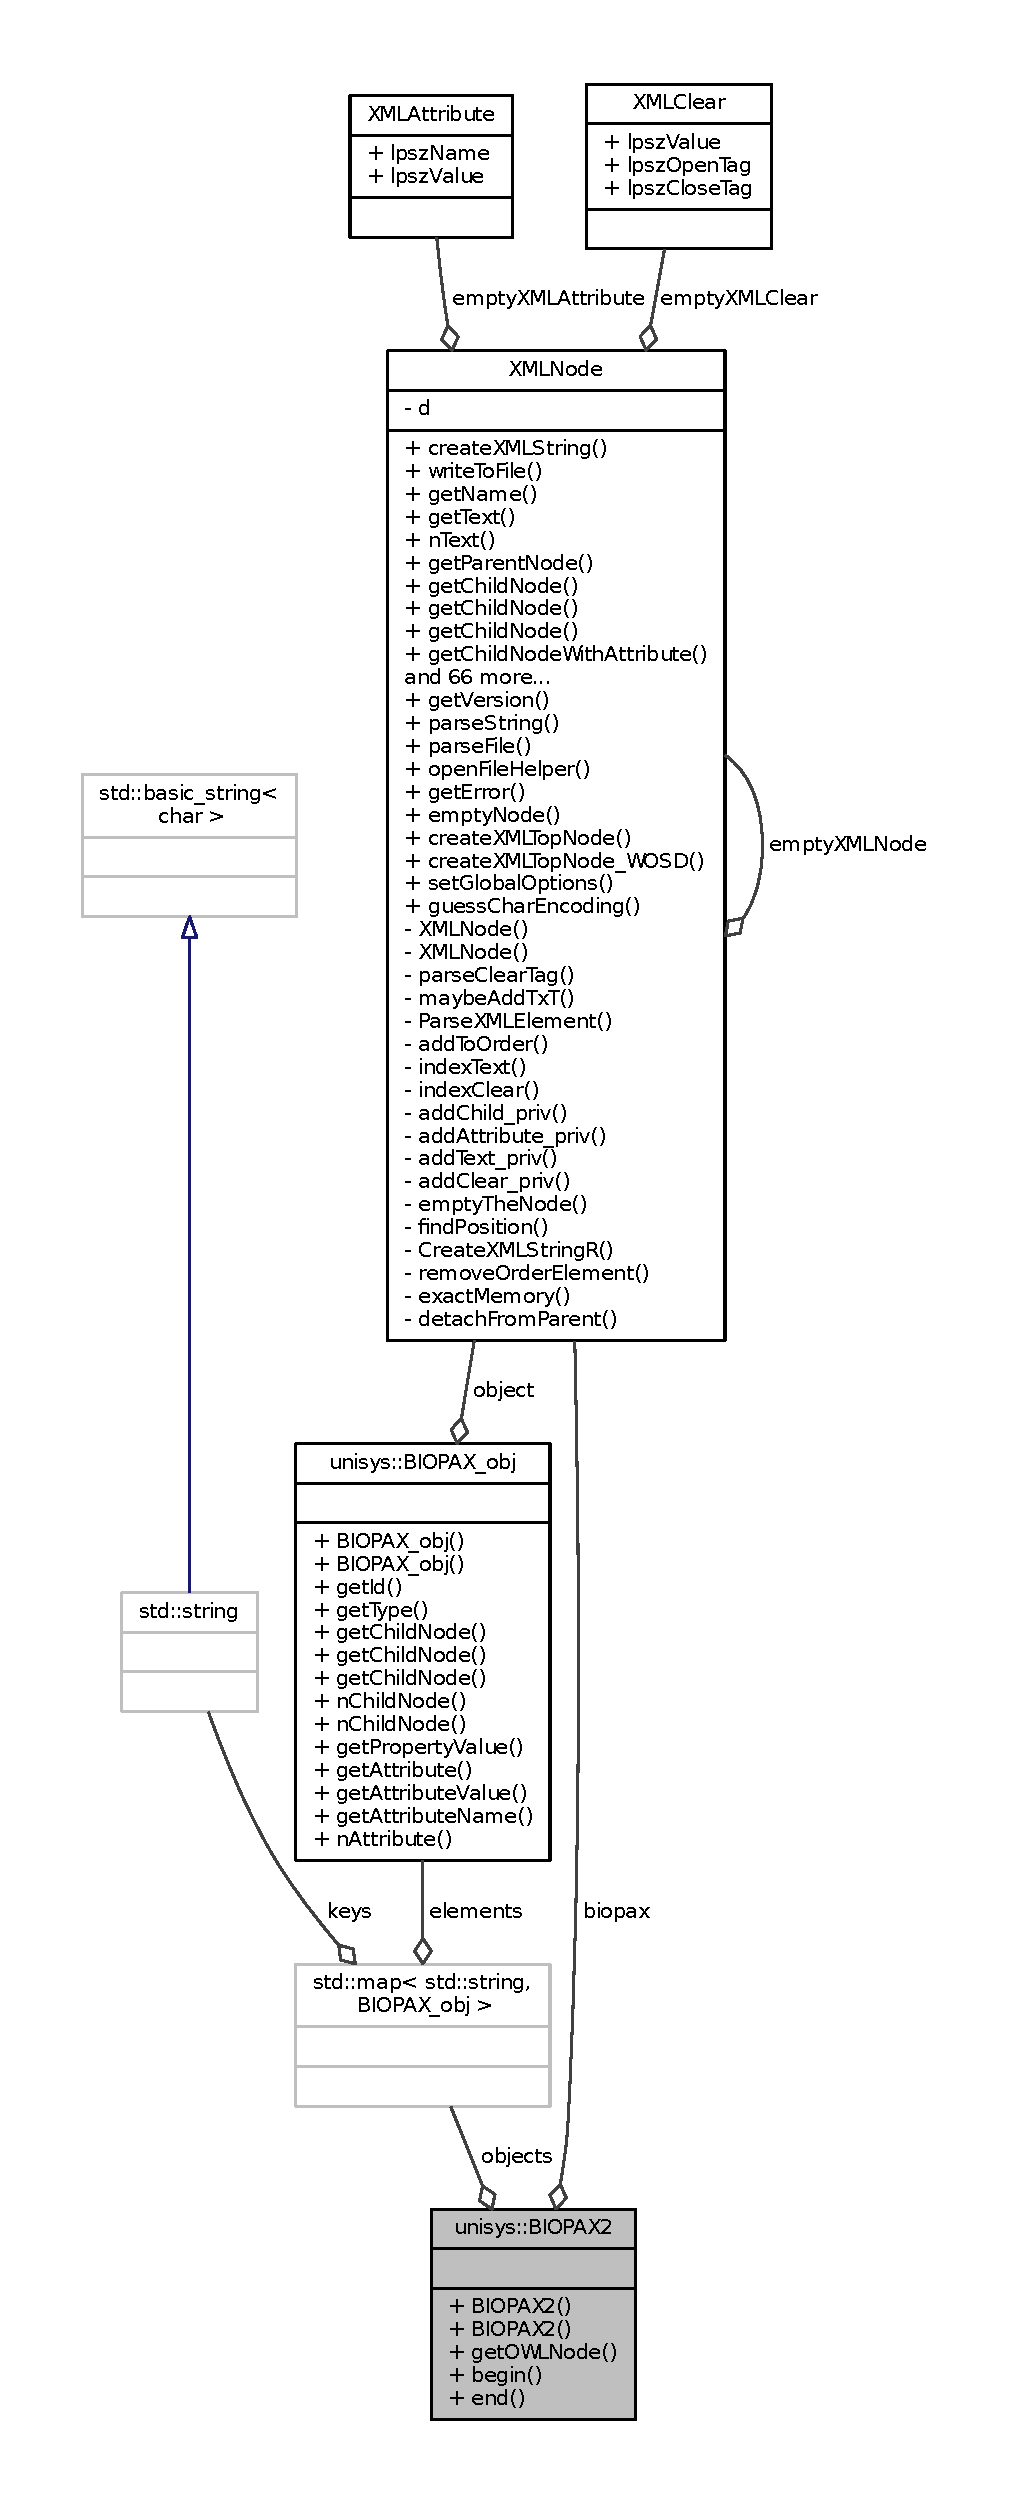
\includegraphics[height=550pt]{classunisys_1_1BIOPAX2__coll__graph}
\end{center}
\end{figure}
\subsection*{Public Types}
\begin{DoxyCompactItemize}
\item 
typedef std\-::map$<$ std\-::string, \\*
\hyperlink{classunisys_1_1BIOPAX__obj}{B\-I\-O\-P\-A\-X\-\_\-obj} $>$ \hyperlink{classunisys_1_1BIOPAX2_afc4e3a4ce60303565431949e09527ba3}{biopax\-Obj\-Map}
\end{DoxyCompactItemize}
\subsection*{Public Member Functions}
\begin{DoxyCompactItemize}
\item 
\hyperlink{classunisys_1_1BIOPAX2_a05bdb19fae62f0a4826c6a83bf1cb63b}{B\-I\-O\-P\-A\-X2} ()
\begin{DoxyCompactList}\small\item\em Defualt constructor. \end{DoxyCompactList}\item 
\hyperlink{classunisys_1_1BIOPAX2_a012b1c9a86e129648cc67c7791703aa5}{B\-I\-O\-P\-A\-X2} (std\-::string file\-Name)
\begin{DoxyCompactList}\small\item\em Constructor with file\-Name as parameter. \end{DoxyCompactList}\item 
\hyperlink{structXMLNode}{X\-M\-L\-Node} \hyperlink{classunisys_1_1BIOPAX2_a355067caeb9981702d1c4a73ab5e9fa3}{get\-O\-W\-L\-Node} () const 
\item 
biopax\-Obj\-Map\-::const\-\_\-iterator \hyperlink{classunisys_1_1BIOPAX2_aeaa3de452a37cdf4850289f6d12eeb29}{begin} () const 
\item 
biopax\-Obj\-Map\-::const\-\_\-iterator \hyperlink{classunisys_1_1BIOPAX2_a6592a5950bb80975a0628d439813e1eb}{end} () const 
\end{DoxyCompactItemize}
\subsection*{Private Attributes}
\begin{DoxyCompactItemize}
\item 
\hyperlink{structXMLNode}{X\-M\-L\-Node} \hyperlink{classunisys_1_1BIOPAX2_adbffce99fec989b7e1318bffdb88697a}{biopax}
\item 
std\-::map$<$ std\-::string, \hyperlink{classunisys_1_1BIOPAX__obj}{B\-I\-O\-P\-A\-X\-\_\-obj} $>$ \hyperlink{classunisys_1_1BIOPAX2_aaa492741eb15232183400166a123f94d}{objects}
\begin{DoxyCompactList}\small\item\em All objects map with their ids. \end{DoxyCompactList}\end{DoxyCompactItemize}


\subsection{Detailed Description}
This class is used to parse O\-W\-L format. 

Data structure using to store information from Tag-\/\-Value pair line except; name and id tag 

\subsection{Member Typedef Documentation}
\hypertarget{classunisys_1_1BIOPAX2_afc4e3a4ce60303565431949e09527ba3}{\index{unisys\-::\-B\-I\-O\-P\-A\-X2@{unisys\-::\-B\-I\-O\-P\-A\-X2}!biopax\-Obj\-Map@{biopax\-Obj\-Map}}
\index{biopax\-Obj\-Map@{biopax\-Obj\-Map}!unisys::BIOPAX2@{unisys\-::\-B\-I\-O\-P\-A\-X2}}
\subsubsection[{biopax\-Obj\-Map}]{\setlength{\rightskip}{0pt plus 5cm}typedef std\-::map$<$std\-::string, {\bf B\-I\-O\-P\-A\-X\-\_\-obj}$>$ {\bf unisys\-::\-B\-I\-O\-P\-A\-X2\-::biopax\-Obj\-Map}}}\label{classunisys_1_1BIOPAX2_afc4e3a4ce60303565431949e09527ba3}


\subsection{Constructor \& Destructor Documentation}
\hypertarget{classunisys_1_1BIOPAX2_a05bdb19fae62f0a4826c6a83bf1cb63b}{\index{unisys\-::\-B\-I\-O\-P\-A\-X2@{unisys\-::\-B\-I\-O\-P\-A\-X2}!B\-I\-O\-P\-A\-X2@{B\-I\-O\-P\-A\-X2}}
\index{B\-I\-O\-P\-A\-X2@{B\-I\-O\-P\-A\-X2}!unisys::BIOPAX2@{unisys\-::\-B\-I\-O\-P\-A\-X2}}
\subsubsection[{B\-I\-O\-P\-A\-X2}]{\setlength{\rightskip}{0pt plus 5cm}unisys\-::\-B\-I\-O\-P\-A\-X2\-::\-B\-I\-O\-P\-A\-X2 (
\begin{DoxyParamCaption}
{}
\end{DoxyParamCaption}
)}}\label{classunisys_1_1BIOPAX2_a05bdb19fae62f0a4826c6a83bf1cb63b}


Defualt constructor. 

\hypertarget{classunisys_1_1BIOPAX2_a012b1c9a86e129648cc67c7791703aa5}{\index{unisys\-::\-B\-I\-O\-P\-A\-X2@{unisys\-::\-B\-I\-O\-P\-A\-X2}!B\-I\-O\-P\-A\-X2@{B\-I\-O\-P\-A\-X2}}
\index{B\-I\-O\-P\-A\-X2@{B\-I\-O\-P\-A\-X2}!unisys::BIOPAX2@{unisys\-::\-B\-I\-O\-P\-A\-X2}}
\subsubsection[{B\-I\-O\-P\-A\-X2}]{\setlength{\rightskip}{0pt plus 5cm}unisys\-::\-B\-I\-O\-P\-A\-X2\-::\-B\-I\-O\-P\-A\-X2 (
\begin{DoxyParamCaption}
\item[{std\-::string}]{file\-Name}
\end{DoxyParamCaption}
)}}\label{classunisys_1_1BIOPAX2_a012b1c9a86e129648cc67c7791703aa5}


Constructor with file\-Name as parameter. 



\subsection{Member Function Documentation}
\hypertarget{classunisys_1_1BIOPAX2_aeaa3de452a37cdf4850289f6d12eeb29}{\index{unisys\-::\-B\-I\-O\-P\-A\-X2@{unisys\-::\-B\-I\-O\-P\-A\-X2}!begin@{begin}}
\index{begin@{begin}!unisys::BIOPAX2@{unisys\-::\-B\-I\-O\-P\-A\-X2}}
\subsubsection[{begin}]{\setlength{\rightskip}{0pt plus 5cm}biopax\-Obj\-Map\-::const\-\_\-iterator unisys\-::\-B\-I\-O\-P\-A\-X2\-::begin (
\begin{DoxyParamCaption}
{}
\end{DoxyParamCaption}
) const}}\label{classunisys_1_1BIOPAX2_aeaa3de452a37cdf4850289f6d12eeb29}
\hypertarget{classunisys_1_1BIOPAX2_a6592a5950bb80975a0628d439813e1eb}{\index{unisys\-::\-B\-I\-O\-P\-A\-X2@{unisys\-::\-B\-I\-O\-P\-A\-X2}!end@{end}}
\index{end@{end}!unisys::BIOPAX2@{unisys\-::\-B\-I\-O\-P\-A\-X2}}
\subsubsection[{end}]{\setlength{\rightskip}{0pt plus 5cm}biopax\-Obj\-Map\-::const\-\_\-iterator unisys\-::\-B\-I\-O\-P\-A\-X2\-::end (
\begin{DoxyParamCaption}
{}
\end{DoxyParamCaption}
) const}}\label{classunisys_1_1BIOPAX2_a6592a5950bb80975a0628d439813e1eb}
\hypertarget{classunisys_1_1BIOPAX2_a355067caeb9981702d1c4a73ab5e9fa3}{\index{unisys\-::\-B\-I\-O\-P\-A\-X2@{unisys\-::\-B\-I\-O\-P\-A\-X2}!get\-O\-W\-L\-Node@{get\-O\-W\-L\-Node}}
\index{get\-O\-W\-L\-Node@{get\-O\-W\-L\-Node}!unisys::BIOPAX2@{unisys\-::\-B\-I\-O\-P\-A\-X2}}
\subsubsection[{get\-O\-W\-L\-Node}]{\setlength{\rightskip}{0pt plus 5cm}{\bf X\-M\-L\-Node} unisys\-::\-B\-I\-O\-P\-A\-X2\-::get\-O\-W\-L\-Node (
\begin{DoxyParamCaption}
{}
\end{DoxyParamCaption}
) const}}\label{classunisys_1_1BIOPAX2_a355067caeb9981702d1c4a73ab5e9fa3}


\subsection{Member Data Documentation}
\hypertarget{classunisys_1_1BIOPAX2_adbffce99fec989b7e1318bffdb88697a}{\index{unisys\-::\-B\-I\-O\-P\-A\-X2@{unisys\-::\-B\-I\-O\-P\-A\-X2}!biopax@{biopax}}
\index{biopax@{biopax}!unisys::BIOPAX2@{unisys\-::\-B\-I\-O\-P\-A\-X2}}
\subsubsection[{biopax}]{\setlength{\rightskip}{0pt plus 5cm}{\bf X\-M\-L\-Node} unisys\-::\-B\-I\-O\-P\-A\-X2\-::biopax\hspace{0.3cm}{\ttfamily [private]}}}\label{classunisys_1_1BIOPAX2_adbffce99fec989b7e1318bffdb88697a}
\hypertarget{classunisys_1_1BIOPAX2_aaa492741eb15232183400166a123f94d}{\index{unisys\-::\-B\-I\-O\-P\-A\-X2@{unisys\-::\-B\-I\-O\-P\-A\-X2}!objects@{objects}}
\index{objects@{objects}!unisys::BIOPAX2@{unisys\-::\-B\-I\-O\-P\-A\-X2}}
\subsubsection[{objects}]{\setlength{\rightskip}{0pt plus 5cm}std\-::map$<$std\-::string, {\bf B\-I\-O\-P\-A\-X\-\_\-obj}$>$ unisys\-::\-B\-I\-O\-P\-A\-X2\-::objects\hspace{0.3cm}{\ttfamily [private]}}}\label{classunisys_1_1BIOPAX2_aaa492741eb15232183400166a123f94d}


All objects map with their ids. 



The documentation for this class was generated from the following file\-:\begin{DoxyCompactItemize}
\item 
\hyperlink{biopax_8h}{biopax.\-h}\end{DoxyCompactItemize}

\hypertarget{classunisys_1_1BIOPAX__obj}{\section{unisys\-:\-:B\-I\-O\-P\-A\-X\-\_\-obj Class Reference}
\label{classunisys_1_1BIOPAX__obj}\index{unisys\-::\-B\-I\-O\-P\-A\-X\-\_\-obj@{unisys\-::\-B\-I\-O\-P\-A\-X\-\_\-obj}}
}


This class is used to parse O\-W\-L format.  




{\ttfamily \#include $<$biopax.\-h$>$}



Collaboration diagram for unisys\-:\-:B\-I\-O\-P\-A\-X\-\_\-obj\-:
\nopagebreak
\begin{figure}[H]
\begin{center}
\leavevmode
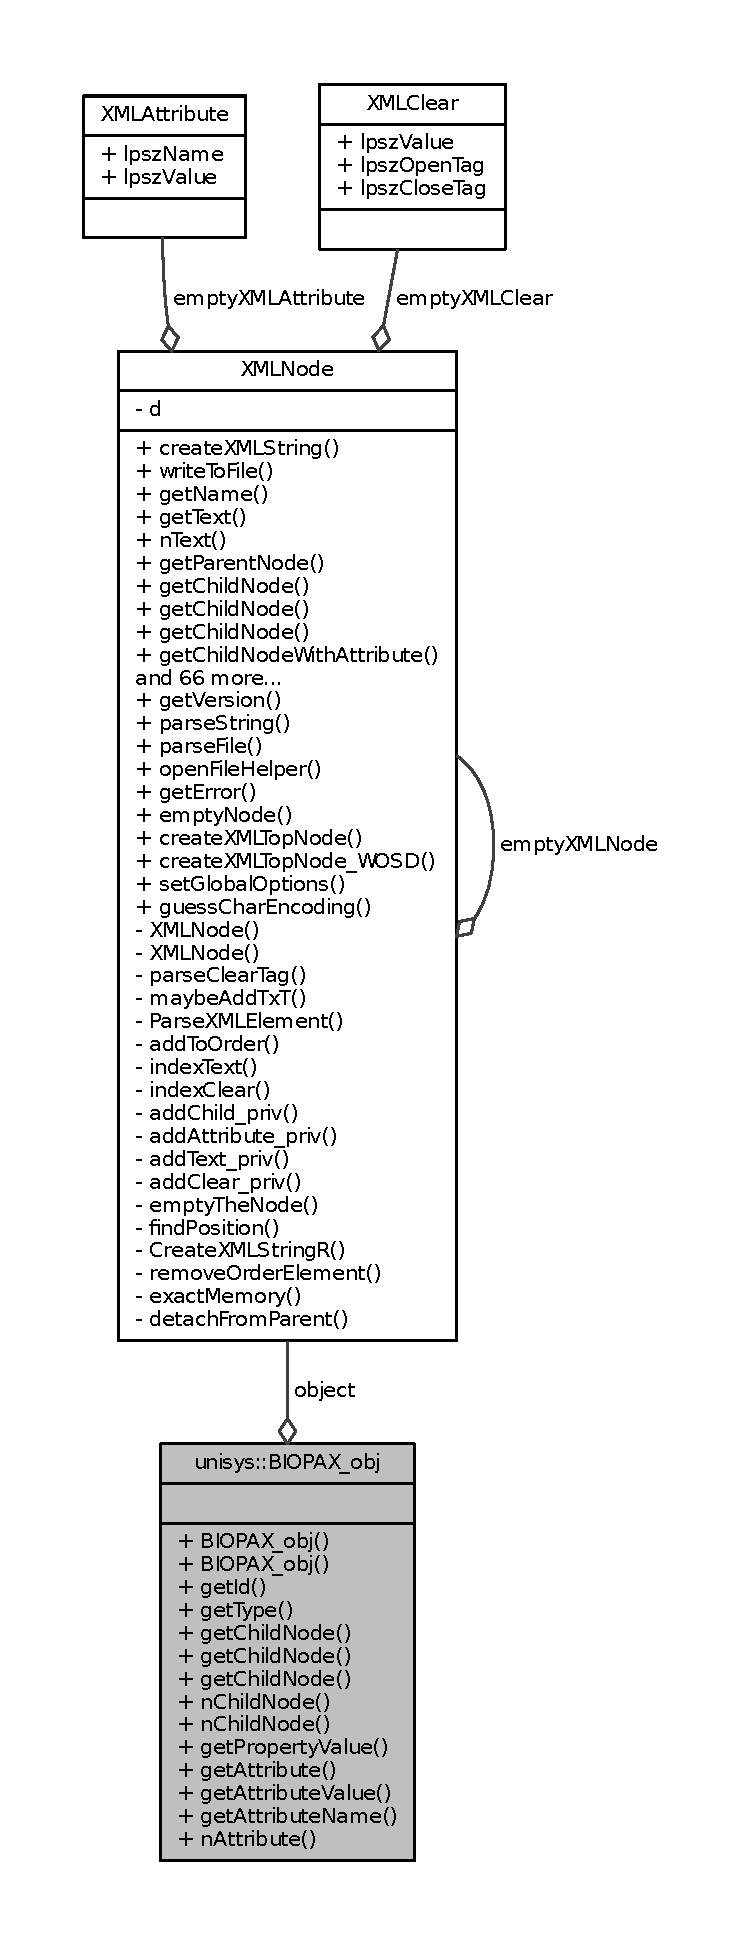
\includegraphics[height=550pt]{classunisys_1_1BIOPAX__obj__coll__graph}
\end{center}
\end{figure}
\subsection*{Public Member Functions}
\begin{DoxyCompactItemize}
\item 
\hyperlink{classunisys_1_1BIOPAX__obj_a4b3addbe446cd1407297942edc9d4241}{B\-I\-O\-P\-A\-X\-\_\-obj} ()
\begin{DoxyCompactList}\small\item\em Defualt constructor. \end{DoxyCompactList}\item 
\hyperlink{classunisys_1_1BIOPAX__obj_a782d016f1b5b5473cf4a871740242d6c}{B\-I\-O\-P\-A\-X\-\_\-obj} (\hyperlink{structXMLNode}{X\-M\-L\-Node} node)
\item 
std\-::string \hyperlink{classunisys_1_1BIOPAX__obj_aab0b0ed0fa5ea280af2082fa17d2667b}{get\-Id} () const 
\item 
std\-::string \hyperlink{classunisys_1_1BIOPAX__obj_ab909dfd9a95c60b5a826d228187741ff}{get\-Type} () const 
\item 
\hyperlink{structXMLNode}{X\-M\-L\-Node} \hyperlink{classunisys_1_1BIOPAX__obj_a1c847f963c9fcb1377ea35a1eeffc1fb}{get\-Child\-Node} (int i=0) const 
\item 
\hyperlink{structXMLNode}{X\-M\-L\-Node} \hyperlink{classunisys_1_1BIOPAX__obj_a21ca7b5d9ce6c932cf3def1768659402}{get\-Child\-Node} (std\-::string name, int i) const 
\item 
\hyperlink{structXMLNode}{X\-M\-L\-Node} \hyperlink{classunisys_1_1BIOPAX__obj_ac426e52509f9f242cf9e4da4ad888302}{get\-Child\-Node} (std\-::string name) const 
\item 
int \hyperlink{classunisys_1_1BIOPAX__obj_af5fe9ed5f554f9b531096e2c8730d341}{n\-Child\-Node} () const 
\item 
int \hyperlink{classunisys_1_1BIOPAX__obj_a35ea6c7c1dcf7f8301c984cfe23aa455}{n\-Child\-Node} (std\-::string name) const 
\item 
std\-::string \hyperlink{classunisys_1_1BIOPAX__obj_a123c67a39d7e9a13bb7fd04b53184590}{get\-Property\-Value} (std\-::string name) const 
\item 
\hyperlink{structXMLAttribute}{X\-M\-L\-Attribute} \hyperlink{classunisys_1_1BIOPAX__obj_a9b73fc23de3e6d71637e254ce2076b21}{get\-Attribute} (int i=0) const 
\item 
std\-::string \hyperlink{classunisys_1_1BIOPAX__obj_ae853daef65696243d402ba2e9c375c7a}{get\-Attribute\-Value} (int i=0) const 
\item 
std\-::string \hyperlink{classunisys_1_1BIOPAX__obj_a3bc3fea7bdb5f60200cebde5406a5ec4}{get\-Attribute\-Name} (int i=0) const 
\item 
int \hyperlink{classunisys_1_1BIOPAX__obj_a6b13a03cba244ce45036ae67da132f83}{n\-Attribute} () const 
\end{DoxyCompactItemize}
\subsection*{Private Attributes}
\begin{DoxyCompactItemize}
\item 
\hyperlink{structXMLNode}{X\-M\-L\-Node} \hyperlink{classunisys_1_1BIOPAX__obj_a27611f048b9ca1852f8aa9a392445128}{object}
\end{DoxyCompactItemize}


\subsection{Detailed Description}
This class is used to parse O\-W\-L format. 

some description. 

\subsection{Constructor \& Destructor Documentation}
\hypertarget{classunisys_1_1BIOPAX__obj_a4b3addbe446cd1407297942edc9d4241}{\index{unisys\-::\-B\-I\-O\-P\-A\-X\-\_\-obj@{unisys\-::\-B\-I\-O\-P\-A\-X\-\_\-obj}!B\-I\-O\-P\-A\-X\-\_\-obj@{B\-I\-O\-P\-A\-X\-\_\-obj}}
\index{B\-I\-O\-P\-A\-X\-\_\-obj@{B\-I\-O\-P\-A\-X\-\_\-obj}!unisys::BIOPAX_obj@{unisys\-::\-B\-I\-O\-P\-A\-X\-\_\-obj}}
\subsubsection[{B\-I\-O\-P\-A\-X\-\_\-obj}]{\setlength{\rightskip}{0pt plus 5cm}unisys\-::\-B\-I\-O\-P\-A\-X\-\_\-obj\-::\-B\-I\-O\-P\-A\-X\-\_\-obj (
\begin{DoxyParamCaption}
{}
\end{DoxyParamCaption}
)}}\label{classunisys_1_1BIOPAX__obj_a4b3addbe446cd1407297942edc9d4241}


Defualt constructor. 

\hypertarget{classunisys_1_1BIOPAX__obj_a782d016f1b5b5473cf4a871740242d6c}{\index{unisys\-::\-B\-I\-O\-P\-A\-X\-\_\-obj@{unisys\-::\-B\-I\-O\-P\-A\-X\-\_\-obj}!B\-I\-O\-P\-A\-X\-\_\-obj@{B\-I\-O\-P\-A\-X\-\_\-obj}}
\index{B\-I\-O\-P\-A\-X\-\_\-obj@{B\-I\-O\-P\-A\-X\-\_\-obj}!unisys::BIOPAX_obj@{unisys\-::\-B\-I\-O\-P\-A\-X\-\_\-obj}}
\subsubsection[{B\-I\-O\-P\-A\-X\-\_\-obj}]{\setlength{\rightskip}{0pt plus 5cm}unisys\-::\-B\-I\-O\-P\-A\-X\-\_\-obj\-::\-B\-I\-O\-P\-A\-X\-\_\-obj (
\begin{DoxyParamCaption}
\item[{{\bf X\-M\-L\-Node}}]{node}
\end{DoxyParamCaption}
)}}\label{classunisys_1_1BIOPAX__obj_a782d016f1b5b5473cf4a871740242d6c}


\subsection{Member Function Documentation}
\hypertarget{classunisys_1_1BIOPAX__obj_a9b73fc23de3e6d71637e254ce2076b21}{\index{unisys\-::\-B\-I\-O\-P\-A\-X\-\_\-obj@{unisys\-::\-B\-I\-O\-P\-A\-X\-\_\-obj}!get\-Attribute@{get\-Attribute}}
\index{get\-Attribute@{get\-Attribute}!unisys::BIOPAX_obj@{unisys\-::\-B\-I\-O\-P\-A\-X\-\_\-obj}}
\subsubsection[{get\-Attribute}]{\setlength{\rightskip}{0pt plus 5cm}{\bf X\-M\-L\-Attribute} unisys\-::\-B\-I\-O\-P\-A\-X\-\_\-obj\-::get\-Attribute (
\begin{DoxyParamCaption}
\item[{int}]{i = {\ttfamily 0}}
\end{DoxyParamCaption}
) const}}\label{classunisys_1_1BIOPAX__obj_a9b73fc23de3e6d71637e254ce2076b21}
\hypertarget{classunisys_1_1BIOPAX__obj_a3bc3fea7bdb5f60200cebde5406a5ec4}{\index{unisys\-::\-B\-I\-O\-P\-A\-X\-\_\-obj@{unisys\-::\-B\-I\-O\-P\-A\-X\-\_\-obj}!get\-Attribute\-Name@{get\-Attribute\-Name}}
\index{get\-Attribute\-Name@{get\-Attribute\-Name}!unisys::BIOPAX_obj@{unisys\-::\-B\-I\-O\-P\-A\-X\-\_\-obj}}
\subsubsection[{get\-Attribute\-Name}]{\setlength{\rightskip}{0pt plus 5cm}std\-::string unisys\-::\-B\-I\-O\-P\-A\-X\-\_\-obj\-::get\-Attribute\-Name (
\begin{DoxyParamCaption}
\item[{int}]{i = {\ttfamily 0}}
\end{DoxyParamCaption}
) const}}\label{classunisys_1_1BIOPAX__obj_a3bc3fea7bdb5f60200cebde5406a5ec4}
\hypertarget{classunisys_1_1BIOPAX__obj_ae853daef65696243d402ba2e9c375c7a}{\index{unisys\-::\-B\-I\-O\-P\-A\-X\-\_\-obj@{unisys\-::\-B\-I\-O\-P\-A\-X\-\_\-obj}!get\-Attribute\-Value@{get\-Attribute\-Value}}
\index{get\-Attribute\-Value@{get\-Attribute\-Value}!unisys::BIOPAX_obj@{unisys\-::\-B\-I\-O\-P\-A\-X\-\_\-obj}}
\subsubsection[{get\-Attribute\-Value}]{\setlength{\rightskip}{0pt plus 5cm}std\-::string unisys\-::\-B\-I\-O\-P\-A\-X\-\_\-obj\-::get\-Attribute\-Value (
\begin{DoxyParamCaption}
\item[{int}]{i = {\ttfamily 0}}
\end{DoxyParamCaption}
) const}}\label{classunisys_1_1BIOPAX__obj_ae853daef65696243d402ba2e9c375c7a}
\hypertarget{classunisys_1_1BIOPAX__obj_a1c847f963c9fcb1377ea35a1eeffc1fb}{\index{unisys\-::\-B\-I\-O\-P\-A\-X\-\_\-obj@{unisys\-::\-B\-I\-O\-P\-A\-X\-\_\-obj}!get\-Child\-Node@{get\-Child\-Node}}
\index{get\-Child\-Node@{get\-Child\-Node}!unisys::BIOPAX_obj@{unisys\-::\-B\-I\-O\-P\-A\-X\-\_\-obj}}
\subsubsection[{get\-Child\-Node}]{\setlength{\rightskip}{0pt plus 5cm}{\bf X\-M\-L\-Node} unisys\-::\-B\-I\-O\-P\-A\-X\-\_\-obj\-::get\-Child\-Node (
\begin{DoxyParamCaption}
\item[{int}]{i = {\ttfamily 0}}
\end{DoxyParamCaption}
) const}}\label{classunisys_1_1BIOPAX__obj_a1c847f963c9fcb1377ea35a1eeffc1fb}
\hypertarget{classunisys_1_1BIOPAX__obj_a21ca7b5d9ce6c932cf3def1768659402}{\index{unisys\-::\-B\-I\-O\-P\-A\-X\-\_\-obj@{unisys\-::\-B\-I\-O\-P\-A\-X\-\_\-obj}!get\-Child\-Node@{get\-Child\-Node}}
\index{get\-Child\-Node@{get\-Child\-Node}!unisys::BIOPAX_obj@{unisys\-::\-B\-I\-O\-P\-A\-X\-\_\-obj}}
\subsubsection[{get\-Child\-Node}]{\setlength{\rightskip}{0pt plus 5cm}{\bf X\-M\-L\-Node} unisys\-::\-B\-I\-O\-P\-A\-X\-\_\-obj\-::get\-Child\-Node (
\begin{DoxyParamCaption}
\item[{std\-::string}]{name, }
\item[{int}]{i}
\end{DoxyParamCaption}
) const}}\label{classunisys_1_1BIOPAX__obj_a21ca7b5d9ce6c932cf3def1768659402}
\hypertarget{classunisys_1_1BIOPAX__obj_ac426e52509f9f242cf9e4da4ad888302}{\index{unisys\-::\-B\-I\-O\-P\-A\-X\-\_\-obj@{unisys\-::\-B\-I\-O\-P\-A\-X\-\_\-obj}!get\-Child\-Node@{get\-Child\-Node}}
\index{get\-Child\-Node@{get\-Child\-Node}!unisys::BIOPAX_obj@{unisys\-::\-B\-I\-O\-P\-A\-X\-\_\-obj}}
\subsubsection[{get\-Child\-Node}]{\setlength{\rightskip}{0pt plus 5cm}{\bf X\-M\-L\-Node} unisys\-::\-B\-I\-O\-P\-A\-X\-\_\-obj\-::get\-Child\-Node (
\begin{DoxyParamCaption}
\item[{std\-::string}]{name}
\end{DoxyParamCaption}
) const}}\label{classunisys_1_1BIOPAX__obj_ac426e52509f9f242cf9e4da4ad888302}
\hypertarget{classunisys_1_1BIOPAX__obj_aab0b0ed0fa5ea280af2082fa17d2667b}{\index{unisys\-::\-B\-I\-O\-P\-A\-X\-\_\-obj@{unisys\-::\-B\-I\-O\-P\-A\-X\-\_\-obj}!get\-Id@{get\-Id}}
\index{get\-Id@{get\-Id}!unisys::BIOPAX_obj@{unisys\-::\-B\-I\-O\-P\-A\-X\-\_\-obj}}
\subsubsection[{get\-Id}]{\setlength{\rightskip}{0pt plus 5cm}std\-::string unisys\-::\-B\-I\-O\-P\-A\-X\-\_\-obj\-::get\-Id (
\begin{DoxyParamCaption}
{}
\end{DoxyParamCaption}
) const}}\label{classunisys_1_1BIOPAX__obj_aab0b0ed0fa5ea280af2082fa17d2667b}
\hypertarget{classunisys_1_1BIOPAX__obj_a123c67a39d7e9a13bb7fd04b53184590}{\index{unisys\-::\-B\-I\-O\-P\-A\-X\-\_\-obj@{unisys\-::\-B\-I\-O\-P\-A\-X\-\_\-obj}!get\-Property\-Value@{get\-Property\-Value}}
\index{get\-Property\-Value@{get\-Property\-Value}!unisys::BIOPAX_obj@{unisys\-::\-B\-I\-O\-P\-A\-X\-\_\-obj}}
\subsubsection[{get\-Property\-Value}]{\setlength{\rightskip}{0pt plus 5cm}std\-::string unisys\-::\-B\-I\-O\-P\-A\-X\-\_\-obj\-::get\-Property\-Value (
\begin{DoxyParamCaption}
\item[{std\-::string}]{name}
\end{DoxyParamCaption}
) const}}\label{classunisys_1_1BIOPAX__obj_a123c67a39d7e9a13bb7fd04b53184590}
\hypertarget{classunisys_1_1BIOPAX__obj_ab909dfd9a95c60b5a826d228187741ff}{\index{unisys\-::\-B\-I\-O\-P\-A\-X\-\_\-obj@{unisys\-::\-B\-I\-O\-P\-A\-X\-\_\-obj}!get\-Type@{get\-Type}}
\index{get\-Type@{get\-Type}!unisys::BIOPAX_obj@{unisys\-::\-B\-I\-O\-P\-A\-X\-\_\-obj}}
\subsubsection[{get\-Type}]{\setlength{\rightskip}{0pt plus 5cm}std\-::string unisys\-::\-B\-I\-O\-P\-A\-X\-\_\-obj\-::get\-Type (
\begin{DoxyParamCaption}
{}
\end{DoxyParamCaption}
) const}}\label{classunisys_1_1BIOPAX__obj_ab909dfd9a95c60b5a826d228187741ff}
\hypertarget{classunisys_1_1BIOPAX__obj_a6b13a03cba244ce45036ae67da132f83}{\index{unisys\-::\-B\-I\-O\-P\-A\-X\-\_\-obj@{unisys\-::\-B\-I\-O\-P\-A\-X\-\_\-obj}!n\-Attribute@{n\-Attribute}}
\index{n\-Attribute@{n\-Attribute}!unisys::BIOPAX_obj@{unisys\-::\-B\-I\-O\-P\-A\-X\-\_\-obj}}
\subsubsection[{n\-Attribute}]{\setlength{\rightskip}{0pt plus 5cm}int unisys\-::\-B\-I\-O\-P\-A\-X\-\_\-obj\-::n\-Attribute (
\begin{DoxyParamCaption}
{}
\end{DoxyParamCaption}
) const}}\label{classunisys_1_1BIOPAX__obj_a6b13a03cba244ce45036ae67da132f83}
\hypertarget{classunisys_1_1BIOPAX__obj_af5fe9ed5f554f9b531096e2c8730d341}{\index{unisys\-::\-B\-I\-O\-P\-A\-X\-\_\-obj@{unisys\-::\-B\-I\-O\-P\-A\-X\-\_\-obj}!n\-Child\-Node@{n\-Child\-Node}}
\index{n\-Child\-Node@{n\-Child\-Node}!unisys::BIOPAX_obj@{unisys\-::\-B\-I\-O\-P\-A\-X\-\_\-obj}}
\subsubsection[{n\-Child\-Node}]{\setlength{\rightskip}{0pt plus 5cm}int unisys\-::\-B\-I\-O\-P\-A\-X\-\_\-obj\-::n\-Child\-Node (
\begin{DoxyParamCaption}
{}
\end{DoxyParamCaption}
) const}}\label{classunisys_1_1BIOPAX__obj_af5fe9ed5f554f9b531096e2c8730d341}
\hypertarget{classunisys_1_1BIOPAX__obj_a35ea6c7c1dcf7f8301c984cfe23aa455}{\index{unisys\-::\-B\-I\-O\-P\-A\-X\-\_\-obj@{unisys\-::\-B\-I\-O\-P\-A\-X\-\_\-obj}!n\-Child\-Node@{n\-Child\-Node}}
\index{n\-Child\-Node@{n\-Child\-Node}!unisys::BIOPAX_obj@{unisys\-::\-B\-I\-O\-P\-A\-X\-\_\-obj}}
\subsubsection[{n\-Child\-Node}]{\setlength{\rightskip}{0pt plus 5cm}int unisys\-::\-B\-I\-O\-P\-A\-X\-\_\-obj\-::n\-Child\-Node (
\begin{DoxyParamCaption}
\item[{std\-::string}]{name}
\end{DoxyParamCaption}
) const}}\label{classunisys_1_1BIOPAX__obj_a35ea6c7c1dcf7f8301c984cfe23aa455}


\subsection{Member Data Documentation}
\hypertarget{classunisys_1_1BIOPAX__obj_a27611f048b9ca1852f8aa9a392445128}{\index{unisys\-::\-B\-I\-O\-P\-A\-X\-\_\-obj@{unisys\-::\-B\-I\-O\-P\-A\-X\-\_\-obj}!object@{object}}
\index{object@{object}!unisys::BIOPAX_obj@{unisys\-::\-B\-I\-O\-P\-A\-X\-\_\-obj}}
\subsubsection[{object}]{\setlength{\rightskip}{0pt plus 5cm}{\bf X\-M\-L\-Node} unisys\-::\-B\-I\-O\-P\-A\-X\-\_\-obj\-::object\hspace{0.3cm}{\ttfamily [private]}}}\label{classunisys_1_1BIOPAX__obj_a27611f048b9ca1852f8aa9a392445128}


The documentation for this class was generated from the following file\-:\begin{DoxyCompactItemize}
\item 
\hyperlink{biopax_8h}{biopax.\-h}\end{DoxyCompactItemize}

\hypertarget{classunisys_1_1BioSource}{\section{unisys\-:\-:Bio\-Source Class Reference}
\label{classunisys_1_1BioSource}\index{unisys\-::\-Bio\-Source@{unisys\-::\-Bio\-Source}}
}


The C++ representative class for Biological Source data class. This class is designed to manage the biological data of source organism.  




{\ttfamily \#include $<$Lit\-Class.\-h$>$}



Inheritance diagram for unisys\-:\-:Bio\-Source\-:
\nopagebreak
\begin{figure}[H]
\begin{center}
\leavevmode
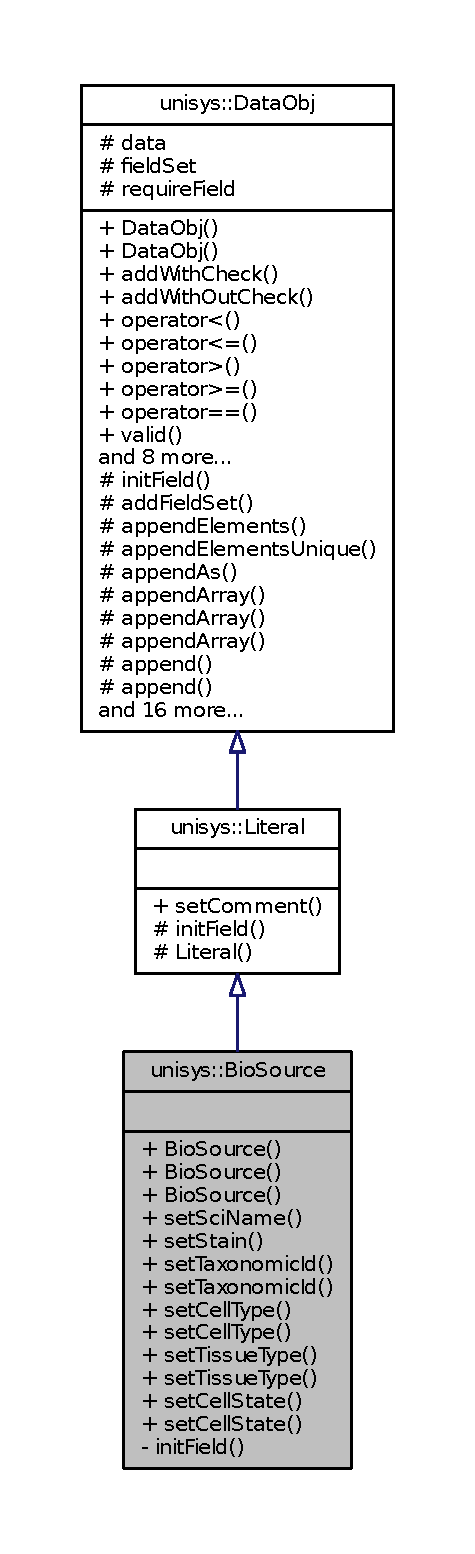
\includegraphics[height=550pt]{classunisys_1_1BioSource__inherit__graph}
\end{center}
\end{figure}


Collaboration diagram for unisys\-:\-:Bio\-Source\-:
\nopagebreak
\begin{figure}[H]
\begin{center}
\leavevmode
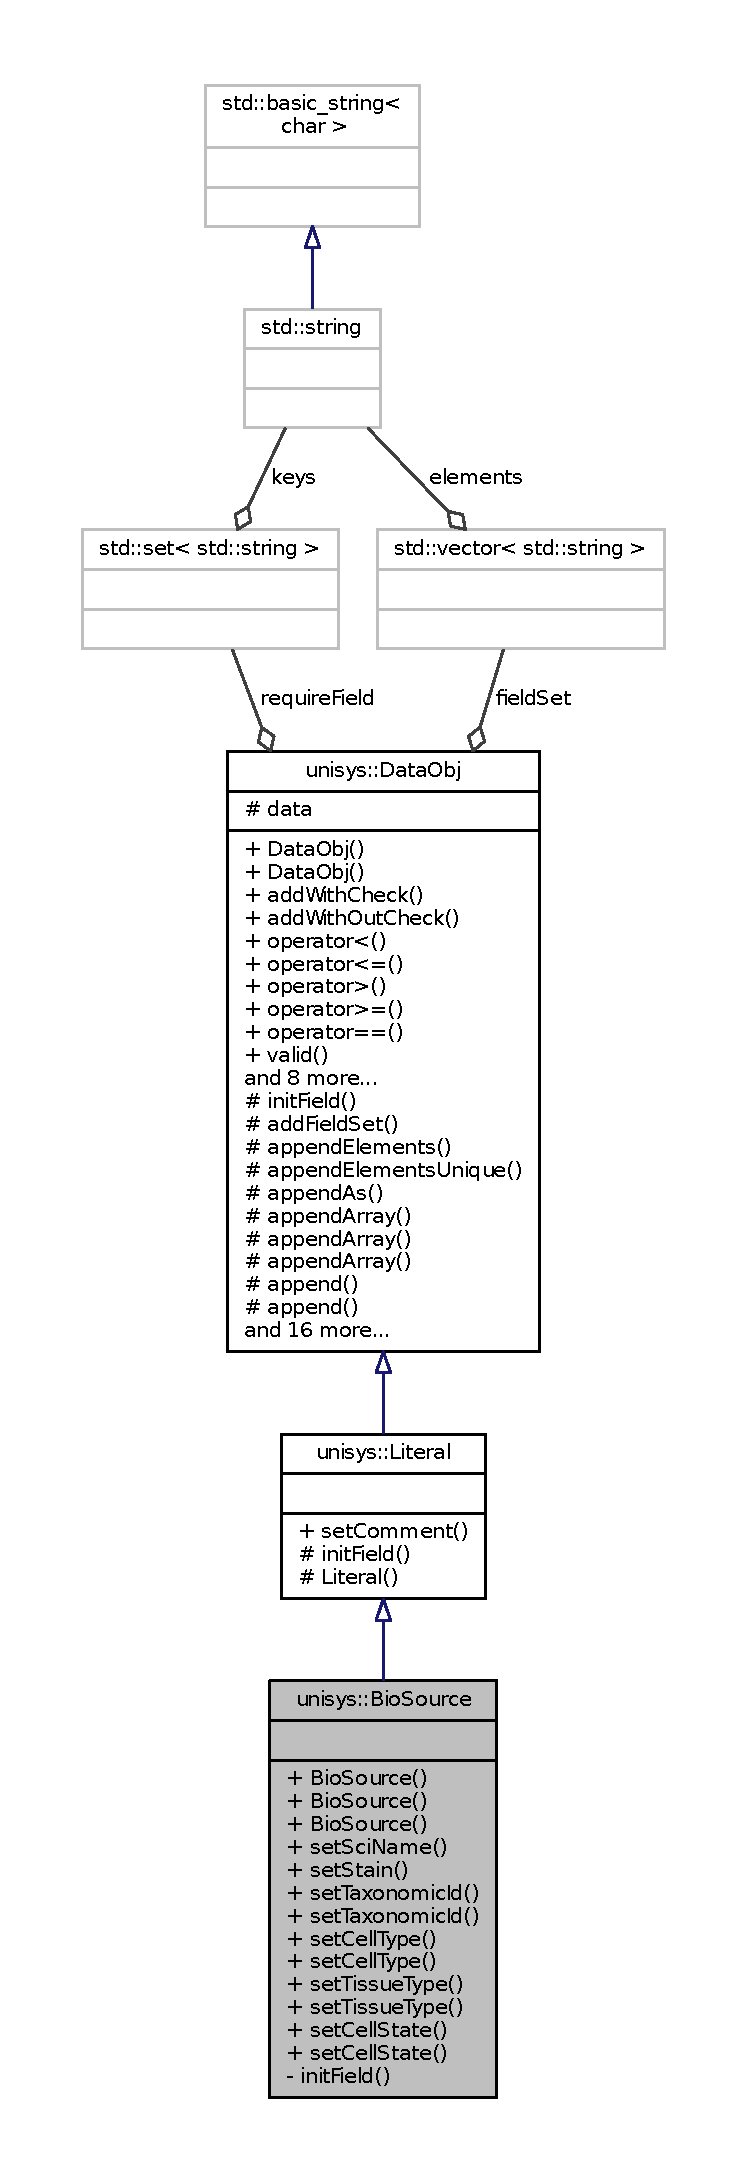
\includegraphics[height=550pt]{classunisys_1_1BioSource__coll__graph}
\end{center}
\end{figure}
\subsection*{Public Member Functions}
\begin{DoxyCompactItemize}
\item 
\hyperlink{classunisys_1_1BioSource_afaab055566a306abfb6ed62a81804114}{Bio\-Source} ()
\begin{DoxyCompactList}\small\item\em Default constructor. \end{DoxyCompactList}\item 
\hyperlink{classunisys_1_1BioSource_a5735f4886634f91d10529995582ea5aa}{Bio\-Source} (mongo\-::\-B\-S\-O\-N\-Obj const \&bson\-Obj)
\begin{DoxyCompactList}\small\item\em Overloaded constructor is used when retriving data in boson object from database and tranform to C++ object. \end{DoxyCompactList}\item 
\hyperlink{classunisys_1_1BioSource_adee19e8a8a7030c47126dc2f2187ef6a}{Bio\-Source} (std\-::string const \&genus, std\-::string const \&species=\char`\"{}.sp\char`\"{})
\item 
void \hyperlink{classunisys_1_1BioSource_a612eb3d5e537c1c91353d0534c099856}{set\-Sci\-Name} (std\-::string const \&genus, std\-::string const \&species=\char`\"{}.sp\char`\"{})
\item 
void \hyperlink{classunisys_1_1BioSource_a804bf9b002185e4becd02314621fb9d5}{set\-Stain} (std\-::string const \&strain)
\item 
void \hyperlink{classunisys_1_1BioSource_a331ad3e04f991ee9cbff05563c52d06f}{set\-Taxonomic\-Id} (\hyperlink{classunisys_1_1Xref}{Xref} \&taxonomic\-Id)
\item 
void \hyperlink{classunisys_1_1BioSource_a4024f5f1324dbb54cc17a449a7a865aa}{set\-Taxonomic\-Id} (std\-::string const \&taxonomic\-Id, std\-::string const \&detail=\char`\"{}\char`\"{})
\item 
void \hyperlink{classunisys_1_1BioSource_afcee59fdda1ffa6ba6123bffaf4bca30}{set\-Cell\-Type} (\hyperlink{classunisys_1_1OntoIdRef}{Onto\-Id\-Ref} \&onto\-Id\-Ref)
\item 
void \hyperlink{classunisys_1_1BioSource_ab66aa67148963a6a37b987ec8ca38cf4}{set\-Cell\-Type} (std\-::string const \&onto\-Id)
\item 
void \hyperlink{classunisys_1_1BioSource_a62c834b403fe514557c99c7cd2a0fe94}{set\-Tissue\-Type} (\hyperlink{classunisys_1_1OntoIdRef}{Onto\-Id\-Ref} \&onto\-Id\-Ref)
\item 
void \hyperlink{classunisys_1_1BioSource_a310667660d177c71b465bcc5f7e967db}{set\-Tissue\-Type} (std\-::string const \&onto\-Id)
\item 
void \hyperlink{classunisys_1_1BioSource_a902f6c3164f677a204e3bbb828f3dde4}{set\-Cell\-State} (\hyperlink{classunisys_1_1OntoIdRef}{Onto\-Id\-Ref} \&onto\-Id\-Ref)
\item 
void \hyperlink{classunisys_1_1BioSource_ac4545f8b833415e88fa734ab0f7e3034}{set\-Cell\-State} (std\-::string const \&onto\-Id)
\end{DoxyCompactItemize}
\subsection*{Private Member Functions}
\begin{DoxyCompactItemize}
\item 
void \hyperlink{classunisys_1_1BioSource_a7a4188b6ce6f969d62c6d903d3e27f09}{init\-Field} ()
\begin{DoxyCompactList}\small\item\em function for init field in the object \end{DoxyCompactList}\end{DoxyCompactItemize}
\subsection*{Additional Inherited Members}


\subsection{Detailed Description}
The C++ representative class for Biological Source data class. This class is designed to manage the biological data of source organism. 

\begin{DoxyVerb}        BSON structure:
        {   
            comment: <string>,
            genus: <string>,
            species: <string>,
            strain: <string>,
            taxonomicId: <XRefBSONStructure>
            cellType: {$ref: <collname>, $id: <idvalue>}, #format by idref class
            tissueType: {$ref: <collname>, $id: <idvalue>}, #format by idref class
            cellState: {$ref: <collname>, $id: <idvalue>}, #format by idref class
        }\end{DoxyVerb}
 

\subsection{Constructor \& Destructor Documentation}
\hypertarget{classunisys_1_1BioSource_afaab055566a306abfb6ed62a81804114}{\index{unisys\-::\-Bio\-Source@{unisys\-::\-Bio\-Source}!Bio\-Source@{Bio\-Source}}
\index{Bio\-Source@{Bio\-Source}!unisys::BioSource@{unisys\-::\-Bio\-Source}}
\subsubsection[{Bio\-Source}]{\setlength{\rightskip}{0pt plus 5cm}unisys\-::\-Bio\-Source\-::\-Bio\-Source (
\begin{DoxyParamCaption}
{}
\end{DoxyParamCaption}
)}}\label{classunisys_1_1BioSource_afaab055566a306abfb6ed62a81804114}


Default constructor. 

\hypertarget{classunisys_1_1BioSource_a5735f4886634f91d10529995582ea5aa}{\index{unisys\-::\-Bio\-Source@{unisys\-::\-Bio\-Source}!Bio\-Source@{Bio\-Source}}
\index{Bio\-Source@{Bio\-Source}!unisys::BioSource@{unisys\-::\-Bio\-Source}}
\subsubsection[{Bio\-Source}]{\setlength{\rightskip}{0pt plus 5cm}unisys\-::\-Bio\-Source\-::\-Bio\-Source (
\begin{DoxyParamCaption}
\item[{mongo\-::\-B\-S\-O\-N\-Obj const \&}]{bson\-Obj}
\end{DoxyParamCaption}
)}}\label{classunisys_1_1BioSource_a5735f4886634f91d10529995582ea5aa}


Overloaded constructor is used when retriving data in boson object from database and tranform to C++ object. 

\hypertarget{classunisys_1_1BioSource_adee19e8a8a7030c47126dc2f2187ef6a}{\index{unisys\-::\-Bio\-Source@{unisys\-::\-Bio\-Source}!Bio\-Source@{Bio\-Source}}
\index{Bio\-Source@{Bio\-Source}!unisys::BioSource@{unisys\-::\-Bio\-Source}}
\subsubsection[{Bio\-Source}]{\setlength{\rightskip}{0pt plus 5cm}unisys\-::\-Bio\-Source\-::\-Bio\-Source (
\begin{DoxyParamCaption}
\item[{std\-::string const \&}]{genus, }
\item[{std\-::string const \&}]{species = {\ttfamily \char`\"{}.sp\char`\"{}}}
\end{DoxyParamCaption}
)}}\label{classunisys_1_1BioSource_adee19e8a8a7030c47126dc2f2187ef6a}


\subsection{Member Function Documentation}
\hypertarget{classunisys_1_1BioSource_a7a4188b6ce6f969d62c6d903d3e27f09}{\index{unisys\-::\-Bio\-Source@{unisys\-::\-Bio\-Source}!init\-Field@{init\-Field}}
\index{init\-Field@{init\-Field}!unisys::BioSource@{unisys\-::\-Bio\-Source}}
\subsubsection[{init\-Field}]{\setlength{\rightskip}{0pt plus 5cm}void unisys\-::\-Bio\-Source\-::init\-Field (
\begin{DoxyParamCaption}
{}
\end{DoxyParamCaption}
)\hspace{0.3cm}{\ttfamily [private]}, {\ttfamily [virtual]}}}\label{classunisys_1_1BioSource_a7a4188b6ce6f969d62c6d903d3e27f09}


function for init field in the object 



Reimplemented from \hyperlink{classunisys_1_1Literal_a769b8f41e99619d8635f83d18a02bc1f}{unisys\-::\-Literal}.

\hypertarget{classunisys_1_1BioSource_a902f6c3164f677a204e3bbb828f3dde4}{\index{unisys\-::\-Bio\-Source@{unisys\-::\-Bio\-Source}!set\-Cell\-State@{set\-Cell\-State}}
\index{set\-Cell\-State@{set\-Cell\-State}!unisys::BioSource@{unisys\-::\-Bio\-Source}}
\subsubsection[{set\-Cell\-State}]{\setlength{\rightskip}{0pt plus 5cm}void unisys\-::\-Bio\-Source\-::set\-Cell\-State (
\begin{DoxyParamCaption}
\item[{{\bf Onto\-Id\-Ref} \&}]{onto\-Id\-Ref}
\end{DoxyParamCaption}
)}}\label{classunisys_1_1BioSource_a902f6c3164f677a204e3bbb828f3dde4}
\hypertarget{classunisys_1_1BioSource_ac4545f8b833415e88fa734ab0f7e3034}{\index{unisys\-::\-Bio\-Source@{unisys\-::\-Bio\-Source}!set\-Cell\-State@{set\-Cell\-State}}
\index{set\-Cell\-State@{set\-Cell\-State}!unisys::BioSource@{unisys\-::\-Bio\-Source}}
\subsubsection[{set\-Cell\-State}]{\setlength{\rightskip}{0pt plus 5cm}void unisys\-::\-Bio\-Source\-::set\-Cell\-State (
\begin{DoxyParamCaption}
\item[{std\-::string const \&}]{onto\-Id}
\end{DoxyParamCaption}
)}}\label{classunisys_1_1BioSource_ac4545f8b833415e88fa734ab0f7e3034}
\hypertarget{classunisys_1_1BioSource_afcee59fdda1ffa6ba6123bffaf4bca30}{\index{unisys\-::\-Bio\-Source@{unisys\-::\-Bio\-Source}!set\-Cell\-Type@{set\-Cell\-Type}}
\index{set\-Cell\-Type@{set\-Cell\-Type}!unisys::BioSource@{unisys\-::\-Bio\-Source}}
\subsubsection[{set\-Cell\-Type}]{\setlength{\rightskip}{0pt plus 5cm}void unisys\-::\-Bio\-Source\-::set\-Cell\-Type (
\begin{DoxyParamCaption}
\item[{{\bf Onto\-Id\-Ref} \&}]{onto\-Id\-Ref}
\end{DoxyParamCaption}
)}}\label{classunisys_1_1BioSource_afcee59fdda1ffa6ba6123bffaf4bca30}
\hypertarget{classunisys_1_1BioSource_ab66aa67148963a6a37b987ec8ca38cf4}{\index{unisys\-::\-Bio\-Source@{unisys\-::\-Bio\-Source}!set\-Cell\-Type@{set\-Cell\-Type}}
\index{set\-Cell\-Type@{set\-Cell\-Type}!unisys::BioSource@{unisys\-::\-Bio\-Source}}
\subsubsection[{set\-Cell\-Type}]{\setlength{\rightskip}{0pt plus 5cm}void unisys\-::\-Bio\-Source\-::set\-Cell\-Type (
\begin{DoxyParamCaption}
\item[{std\-::string const \&}]{onto\-Id}
\end{DoxyParamCaption}
)}}\label{classunisys_1_1BioSource_ab66aa67148963a6a37b987ec8ca38cf4}
\hypertarget{classunisys_1_1BioSource_a612eb3d5e537c1c91353d0534c099856}{\index{unisys\-::\-Bio\-Source@{unisys\-::\-Bio\-Source}!set\-Sci\-Name@{set\-Sci\-Name}}
\index{set\-Sci\-Name@{set\-Sci\-Name}!unisys::BioSource@{unisys\-::\-Bio\-Source}}
\subsubsection[{set\-Sci\-Name}]{\setlength{\rightskip}{0pt plus 5cm}void unisys\-::\-Bio\-Source\-::set\-Sci\-Name (
\begin{DoxyParamCaption}
\item[{std\-::string const \&}]{genus, }
\item[{std\-::string const \&}]{species = {\ttfamily \char`\"{}.sp\char`\"{}}}
\end{DoxyParamCaption}
)}}\label{classunisys_1_1BioSource_a612eb3d5e537c1c91353d0534c099856}
\hypertarget{classunisys_1_1BioSource_a804bf9b002185e4becd02314621fb9d5}{\index{unisys\-::\-Bio\-Source@{unisys\-::\-Bio\-Source}!set\-Stain@{set\-Stain}}
\index{set\-Stain@{set\-Stain}!unisys::BioSource@{unisys\-::\-Bio\-Source}}
\subsubsection[{set\-Stain}]{\setlength{\rightskip}{0pt plus 5cm}void unisys\-::\-Bio\-Source\-::set\-Stain (
\begin{DoxyParamCaption}
\item[{std\-::string const \&}]{strain}
\end{DoxyParamCaption}
)}}\label{classunisys_1_1BioSource_a804bf9b002185e4becd02314621fb9d5}
\hypertarget{classunisys_1_1BioSource_a331ad3e04f991ee9cbff05563c52d06f}{\index{unisys\-::\-Bio\-Source@{unisys\-::\-Bio\-Source}!set\-Taxonomic\-Id@{set\-Taxonomic\-Id}}
\index{set\-Taxonomic\-Id@{set\-Taxonomic\-Id}!unisys::BioSource@{unisys\-::\-Bio\-Source}}
\subsubsection[{set\-Taxonomic\-Id}]{\setlength{\rightskip}{0pt plus 5cm}void unisys\-::\-Bio\-Source\-::set\-Taxonomic\-Id (
\begin{DoxyParamCaption}
\item[{{\bf Xref} \&}]{taxonomic\-Id}
\end{DoxyParamCaption}
)}}\label{classunisys_1_1BioSource_a331ad3e04f991ee9cbff05563c52d06f}
\hypertarget{classunisys_1_1BioSource_a4024f5f1324dbb54cc17a449a7a865aa}{\index{unisys\-::\-Bio\-Source@{unisys\-::\-Bio\-Source}!set\-Taxonomic\-Id@{set\-Taxonomic\-Id}}
\index{set\-Taxonomic\-Id@{set\-Taxonomic\-Id}!unisys::BioSource@{unisys\-::\-Bio\-Source}}
\subsubsection[{set\-Taxonomic\-Id}]{\setlength{\rightskip}{0pt plus 5cm}void unisys\-::\-Bio\-Source\-::set\-Taxonomic\-Id (
\begin{DoxyParamCaption}
\item[{std\-::string const \&}]{taxonomic\-Id, }
\item[{std\-::string const \&}]{detail = {\ttfamily \char`\"{}\char`\"{}}}
\end{DoxyParamCaption}
)}}\label{classunisys_1_1BioSource_a4024f5f1324dbb54cc17a449a7a865aa}
\hypertarget{classunisys_1_1BioSource_a62c834b403fe514557c99c7cd2a0fe94}{\index{unisys\-::\-Bio\-Source@{unisys\-::\-Bio\-Source}!set\-Tissue\-Type@{set\-Tissue\-Type}}
\index{set\-Tissue\-Type@{set\-Tissue\-Type}!unisys::BioSource@{unisys\-::\-Bio\-Source}}
\subsubsection[{set\-Tissue\-Type}]{\setlength{\rightskip}{0pt plus 5cm}void unisys\-::\-Bio\-Source\-::set\-Tissue\-Type (
\begin{DoxyParamCaption}
\item[{{\bf Onto\-Id\-Ref} \&}]{onto\-Id\-Ref}
\end{DoxyParamCaption}
)}}\label{classunisys_1_1BioSource_a62c834b403fe514557c99c7cd2a0fe94}
\hypertarget{classunisys_1_1BioSource_a310667660d177c71b465bcc5f7e967db}{\index{unisys\-::\-Bio\-Source@{unisys\-::\-Bio\-Source}!set\-Tissue\-Type@{set\-Tissue\-Type}}
\index{set\-Tissue\-Type@{set\-Tissue\-Type}!unisys::BioSource@{unisys\-::\-Bio\-Source}}
\subsubsection[{set\-Tissue\-Type}]{\setlength{\rightskip}{0pt plus 5cm}void unisys\-::\-Bio\-Source\-::set\-Tissue\-Type (
\begin{DoxyParamCaption}
\item[{std\-::string const \&}]{onto\-Id}
\end{DoxyParamCaption}
)}}\label{classunisys_1_1BioSource_a310667660d177c71b465bcc5f7e967db}


The documentation for this class was generated from the following file\-:\begin{DoxyCompactItemize}
\item 
\hyperlink{LitClass_8h}{Lit\-Class.\-h}\end{DoxyCompactItemize}

\hypertarget{classunisys_1_1CellularLocation}{\section{unisys\-:\-:Cellular\-Location Class Reference}
\label{classunisys_1_1CellularLocation}\index{unisys\-::\-Cellular\-Location@{unisys\-::\-Cellular\-Location}}
}


The C++ representative class for cellular location data class.  




{\ttfamily \#include $<$Lit\-Class.\-h$>$}



Inheritance diagram for unisys\-:\-:Cellular\-Location\-:
\nopagebreak
\begin{figure}[H]
\begin{center}
\leavevmode
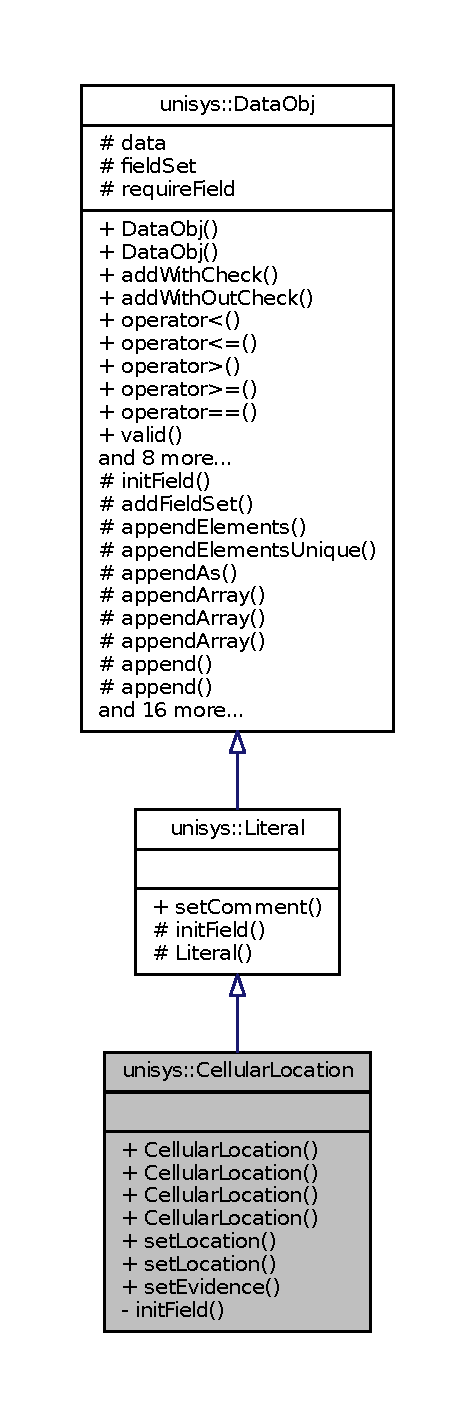
\includegraphics[height=550pt]{classunisys_1_1CellularLocation__inherit__graph}
\end{center}
\end{figure}


Collaboration diagram for unisys\-:\-:Cellular\-Location\-:
\nopagebreak
\begin{figure}[H]
\begin{center}
\leavevmode
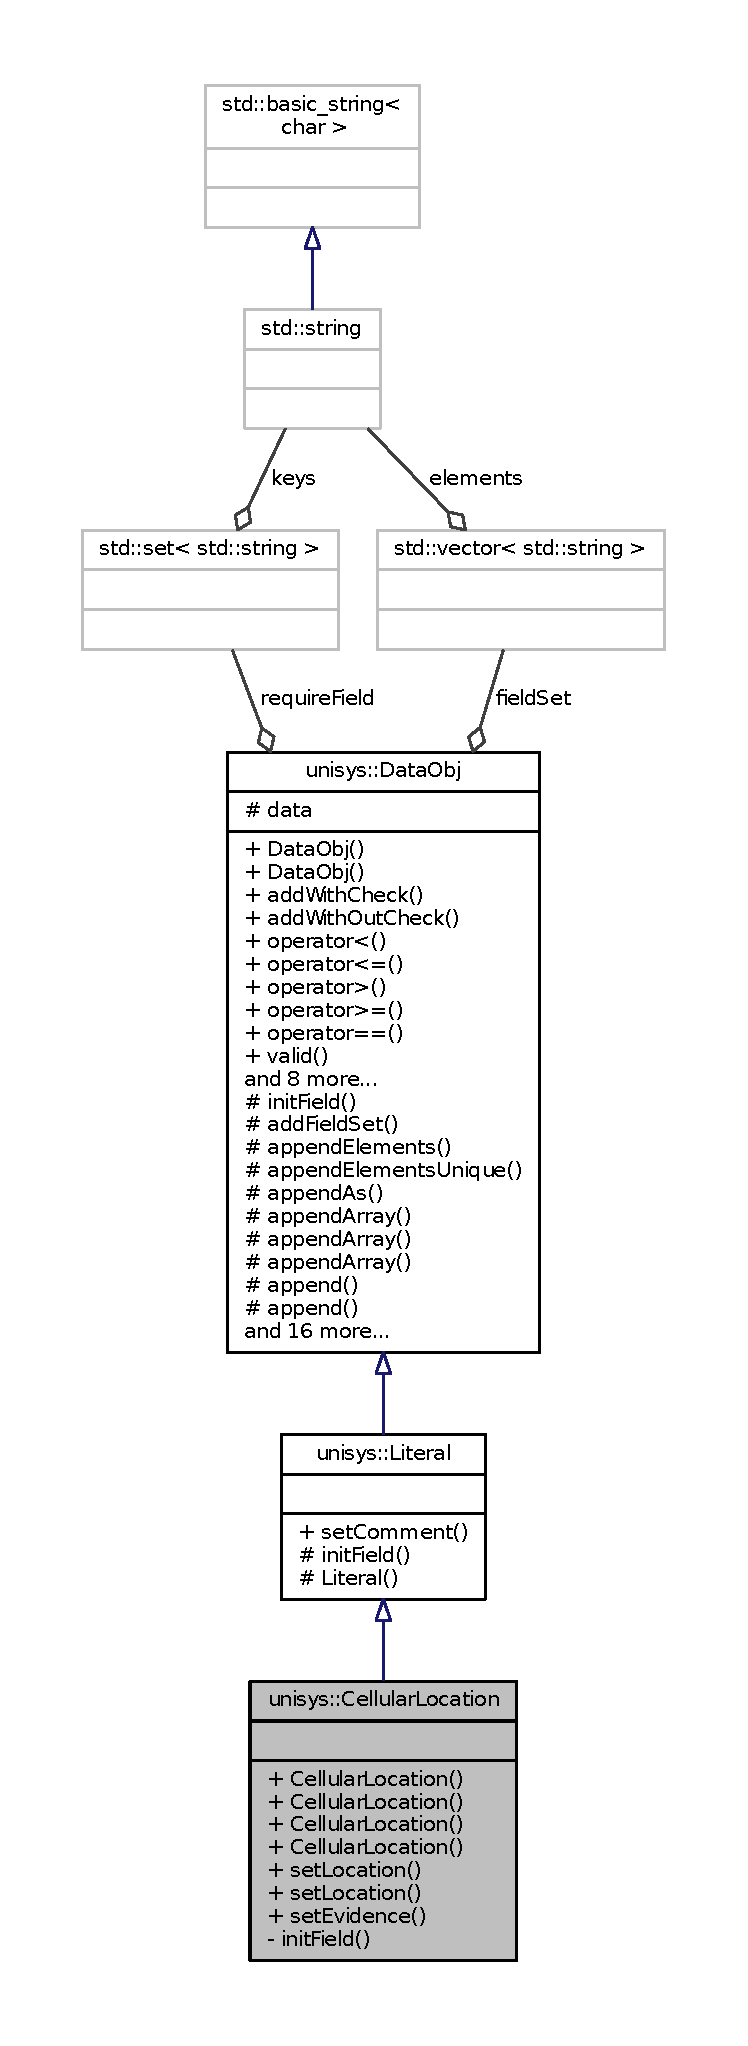
\includegraphics[height=550pt]{classunisys_1_1CellularLocation__coll__graph}
\end{center}
\end{figure}
\subsection*{Public Member Functions}
\begin{DoxyCompactItemize}
\item 
\hyperlink{classunisys_1_1CellularLocation_a46ed7fca62bedc9f3ac621c79eb128bb}{Cellular\-Location} ()
\begin{DoxyCompactList}\small\item\em Default constructor. \end{DoxyCompactList}\item 
\hyperlink{classunisys_1_1CellularLocation_aa9065ea0a1430e686f45b6c124bd1e5c}{Cellular\-Location} (mongo\-::\-B\-S\-O\-N\-Obj const \&bson\-Obj)
\begin{DoxyCompactList}\small\item\em Overloaded constructor is used when retriving data in boson object from database and tranform to C++ object. \end{DoxyCompactList}\item 
\hyperlink{classunisys_1_1CellularLocation_a20b1883b266c82b190ffcddf65b7bd06}{Cellular\-Location} (std\-::string const \&onto\-Id)
\item 
\hyperlink{classunisys_1_1CellularLocation_aa53a8503c5194bdf73754eb43d85679f}{Cellular\-Location} (std\-::string const \&onto\-Id, \hyperlink{classunisys_1_1Evidence}{Evidence} \&evidence)
\item 
void \hyperlink{classunisys_1_1CellularLocation_ac9293b818286bb95c9457dbe5c0d8b2a}{set\-Location} (\hyperlink{classunisys_1_1OntoIdRef}{Onto\-Id\-Ref} \&onto\-Id\-Ref)
\item 
void \hyperlink{classunisys_1_1CellularLocation_a67cdc4c13710e2abbe206883eda1db78}{set\-Location} (std\-::string const \&onto\-Id)
\item 
void \hyperlink{classunisys_1_1CellularLocation_ae19abcc07b3bee3a133125dc550f4414}{set\-Evidence} (\hyperlink{classunisys_1_1Evidence}{Evidence} \&evidence)
\end{DoxyCompactItemize}
\subsection*{Private Member Functions}
\begin{DoxyCompactItemize}
\item 
void \hyperlink{classunisys_1_1CellularLocation_a3aa4c3ebf735ecf9672d0986a63b1dfe}{init\-Field} ()
\begin{DoxyCompactList}\small\item\em function for init field in the object \end{DoxyCompactList}\end{DoxyCompactItemize}
\subsection*{Additional Inherited Members}


\subsection{Detailed Description}
The C++ representative class for cellular location data class. 

\begin{DoxyVerb}        BSON structure:
        {   
            comment: <string>,
            location: {$ref: <collname>, $id: <idvalue>}, #format by idref class
            evidence: <EvidenceBSONStructure>
        }\end{DoxyVerb}
 

\subsection{Constructor \& Destructor Documentation}
\hypertarget{classunisys_1_1CellularLocation_a46ed7fca62bedc9f3ac621c79eb128bb}{\index{unisys\-::\-Cellular\-Location@{unisys\-::\-Cellular\-Location}!Cellular\-Location@{Cellular\-Location}}
\index{Cellular\-Location@{Cellular\-Location}!unisys::CellularLocation@{unisys\-::\-Cellular\-Location}}
\subsubsection[{Cellular\-Location}]{\setlength{\rightskip}{0pt plus 5cm}unisys\-::\-Cellular\-Location\-::\-Cellular\-Location (
\begin{DoxyParamCaption}
{}
\end{DoxyParamCaption}
)}}\label{classunisys_1_1CellularLocation_a46ed7fca62bedc9f3ac621c79eb128bb}


Default constructor. 

\hypertarget{classunisys_1_1CellularLocation_aa9065ea0a1430e686f45b6c124bd1e5c}{\index{unisys\-::\-Cellular\-Location@{unisys\-::\-Cellular\-Location}!Cellular\-Location@{Cellular\-Location}}
\index{Cellular\-Location@{Cellular\-Location}!unisys::CellularLocation@{unisys\-::\-Cellular\-Location}}
\subsubsection[{Cellular\-Location}]{\setlength{\rightskip}{0pt plus 5cm}unisys\-::\-Cellular\-Location\-::\-Cellular\-Location (
\begin{DoxyParamCaption}
\item[{mongo\-::\-B\-S\-O\-N\-Obj const \&}]{bson\-Obj}
\end{DoxyParamCaption}
)}}\label{classunisys_1_1CellularLocation_aa9065ea0a1430e686f45b6c124bd1e5c}


Overloaded constructor is used when retriving data in boson object from database and tranform to C++ object. 

\hypertarget{classunisys_1_1CellularLocation_a20b1883b266c82b190ffcddf65b7bd06}{\index{unisys\-::\-Cellular\-Location@{unisys\-::\-Cellular\-Location}!Cellular\-Location@{Cellular\-Location}}
\index{Cellular\-Location@{Cellular\-Location}!unisys::CellularLocation@{unisys\-::\-Cellular\-Location}}
\subsubsection[{Cellular\-Location}]{\setlength{\rightskip}{0pt plus 5cm}unisys\-::\-Cellular\-Location\-::\-Cellular\-Location (
\begin{DoxyParamCaption}
\item[{std\-::string const \&}]{onto\-Id}
\end{DoxyParamCaption}
)}}\label{classunisys_1_1CellularLocation_a20b1883b266c82b190ffcddf65b7bd06}
\hypertarget{classunisys_1_1CellularLocation_aa53a8503c5194bdf73754eb43d85679f}{\index{unisys\-::\-Cellular\-Location@{unisys\-::\-Cellular\-Location}!Cellular\-Location@{Cellular\-Location}}
\index{Cellular\-Location@{Cellular\-Location}!unisys::CellularLocation@{unisys\-::\-Cellular\-Location}}
\subsubsection[{Cellular\-Location}]{\setlength{\rightskip}{0pt plus 5cm}unisys\-::\-Cellular\-Location\-::\-Cellular\-Location (
\begin{DoxyParamCaption}
\item[{std\-::string const \&}]{onto\-Id, }
\item[{{\bf Evidence} \&}]{evidence}
\end{DoxyParamCaption}
)}}\label{classunisys_1_1CellularLocation_aa53a8503c5194bdf73754eb43d85679f}


\subsection{Member Function Documentation}
\hypertarget{classunisys_1_1CellularLocation_a3aa4c3ebf735ecf9672d0986a63b1dfe}{\index{unisys\-::\-Cellular\-Location@{unisys\-::\-Cellular\-Location}!init\-Field@{init\-Field}}
\index{init\-Field@{init\-Field}!unisys::CellularLocation@{unisys\-::\-Cellular\-Location}}
\subsubsection[{init\-Field}]{\setlength{\rightskip}{0pt plus 5cm}void unisys\-::\-Cellular\-Location\-::init\-Field (
\begin{DoxyParamCaption}
{}
\end{DoxyParamCaption}
)\hspace{0.3cm}{\ttfamily [private]}, {\ttfamily [virtual]}}}\label{classunisys_1_1CellularLocation_a3aa4c3ebf735ecf9672d0986a63b1dfe}


function for init field in the object 



Reimplemented from \hyperlink{classunisys_1_1Literal_a769b8f41e99619d8635f83d18a02bc1f}{unisys\-::\-Literal}.

\hypertarget{classunisys_1_1CellularLocation_ae19abcc07b3bee3a133125dc550f4414}{\index{unisys\-::\-Cellular\-Location@{unisys\-::\-Cellular\-Location}!set\-Evidence@{set\-Evidence}}
\index{set\-Evidence@{set\-Evidence}!unisys::CellularLocation@{unisys\-::\-Cellular\-Location}}
\subsubsection[{set\-Evidence}]{\setlength{\rightskip}{0pt plus 5cm}void unisys\-::\-Cellular\-Location\-::set\-Evidence (
\begin{DoxyParamCaption}
\item[{{\bf Evidence} \&}]{evidence}
\end{DoxyParamCaption}
)}}\label{classunisys_1_1CellularLocation_ae19abcc07b3bee3a133125dc550f4414}
\hypertarget{classunisys_1_1CellularLocation_ac9293b818286bb95c9457dbe5c0d8b2a}{\index{unisys\-::\-Cellular\-Location@{unisys\-::\-Cellular\-Location}!set\-Location@{set\-Location}}
\index{set\-Location@{set\-Location}!unisys::CellularLocation@{unisys\-::\-Cellular\-Location}}
\subsubsection[{set\-Location}]{\setlength{\rightskip}{0pt plus 5cm}void unisys\-::\-Cellular\-Location\-::set\-Location (
\begin{DoxyParamCaption}
\item[{{\bf Onto\-Id\-Ref} \&}]{onto\-Id\-Ref}
\end{DoxyParamCaption}
)}}\label{classunisys_1_1CellularLocation_ac9293b818286bb95c9457dbe5c0d8b2a}
\hypertarget{classunisys_1_1CellularLocation_a67cdc4c13710e2abbe206883eda1db78}{\index{unisys\-::\-Cellular\-Location@{unisys\-::\-Cellular\-Location}!set\-Location@{set\-Location}}
\index{set\-Location@{set\-Location}!unisys::CellularLocation@{unisys\-::\-Cellular\-Location}}
\subsubsection[{set\-Location}]{\setlength{\rightskip}{0pt plus 5cm}void unisys\-::\-Cellular\-Location\-::set\-Location (
\begin{DoxyParamCaption}
\item[{std\-::string const \&}]{onto\-Id}
\end{DoxyParamCaption}
)}}\label{classunisys_1_1CellularLocation_a67cdc4c13710e2abbe206883eda1db78}


The documentation for this class was generated from the following file\-:\begin{DoxyCompactItemize}
\item 
\hyperlink{LitClass_8h}{Lit\-Class.\-h}\end{DoxyCompactItemize}

\hypertarget{classunisys_1_1ChEBIOWL}{\section{unisys\-:\-:Ch\-E\-B\-I\-O\-W\-L Class Reference}
\label{classunisys_1_1ChEBIOWL}\index{unisys\-::\-Ch\-E\-B\-I\-O\-W\-L@{unisys\-::\-Ch\-E\-B\-I\-O\-W\-L}}
}


Used to parse Ch\-E\-B\-I O\-W\-L format.  




{\ttfamily \#include $<$chebiowl.\-h$>$}



Collaboration diagram for unisys\-:\-:Ch\-E\-B\-I\-O\-W\-L\-:
\nopagebreak
\begin{figure}[H]
\begin{center}
\leavevmode
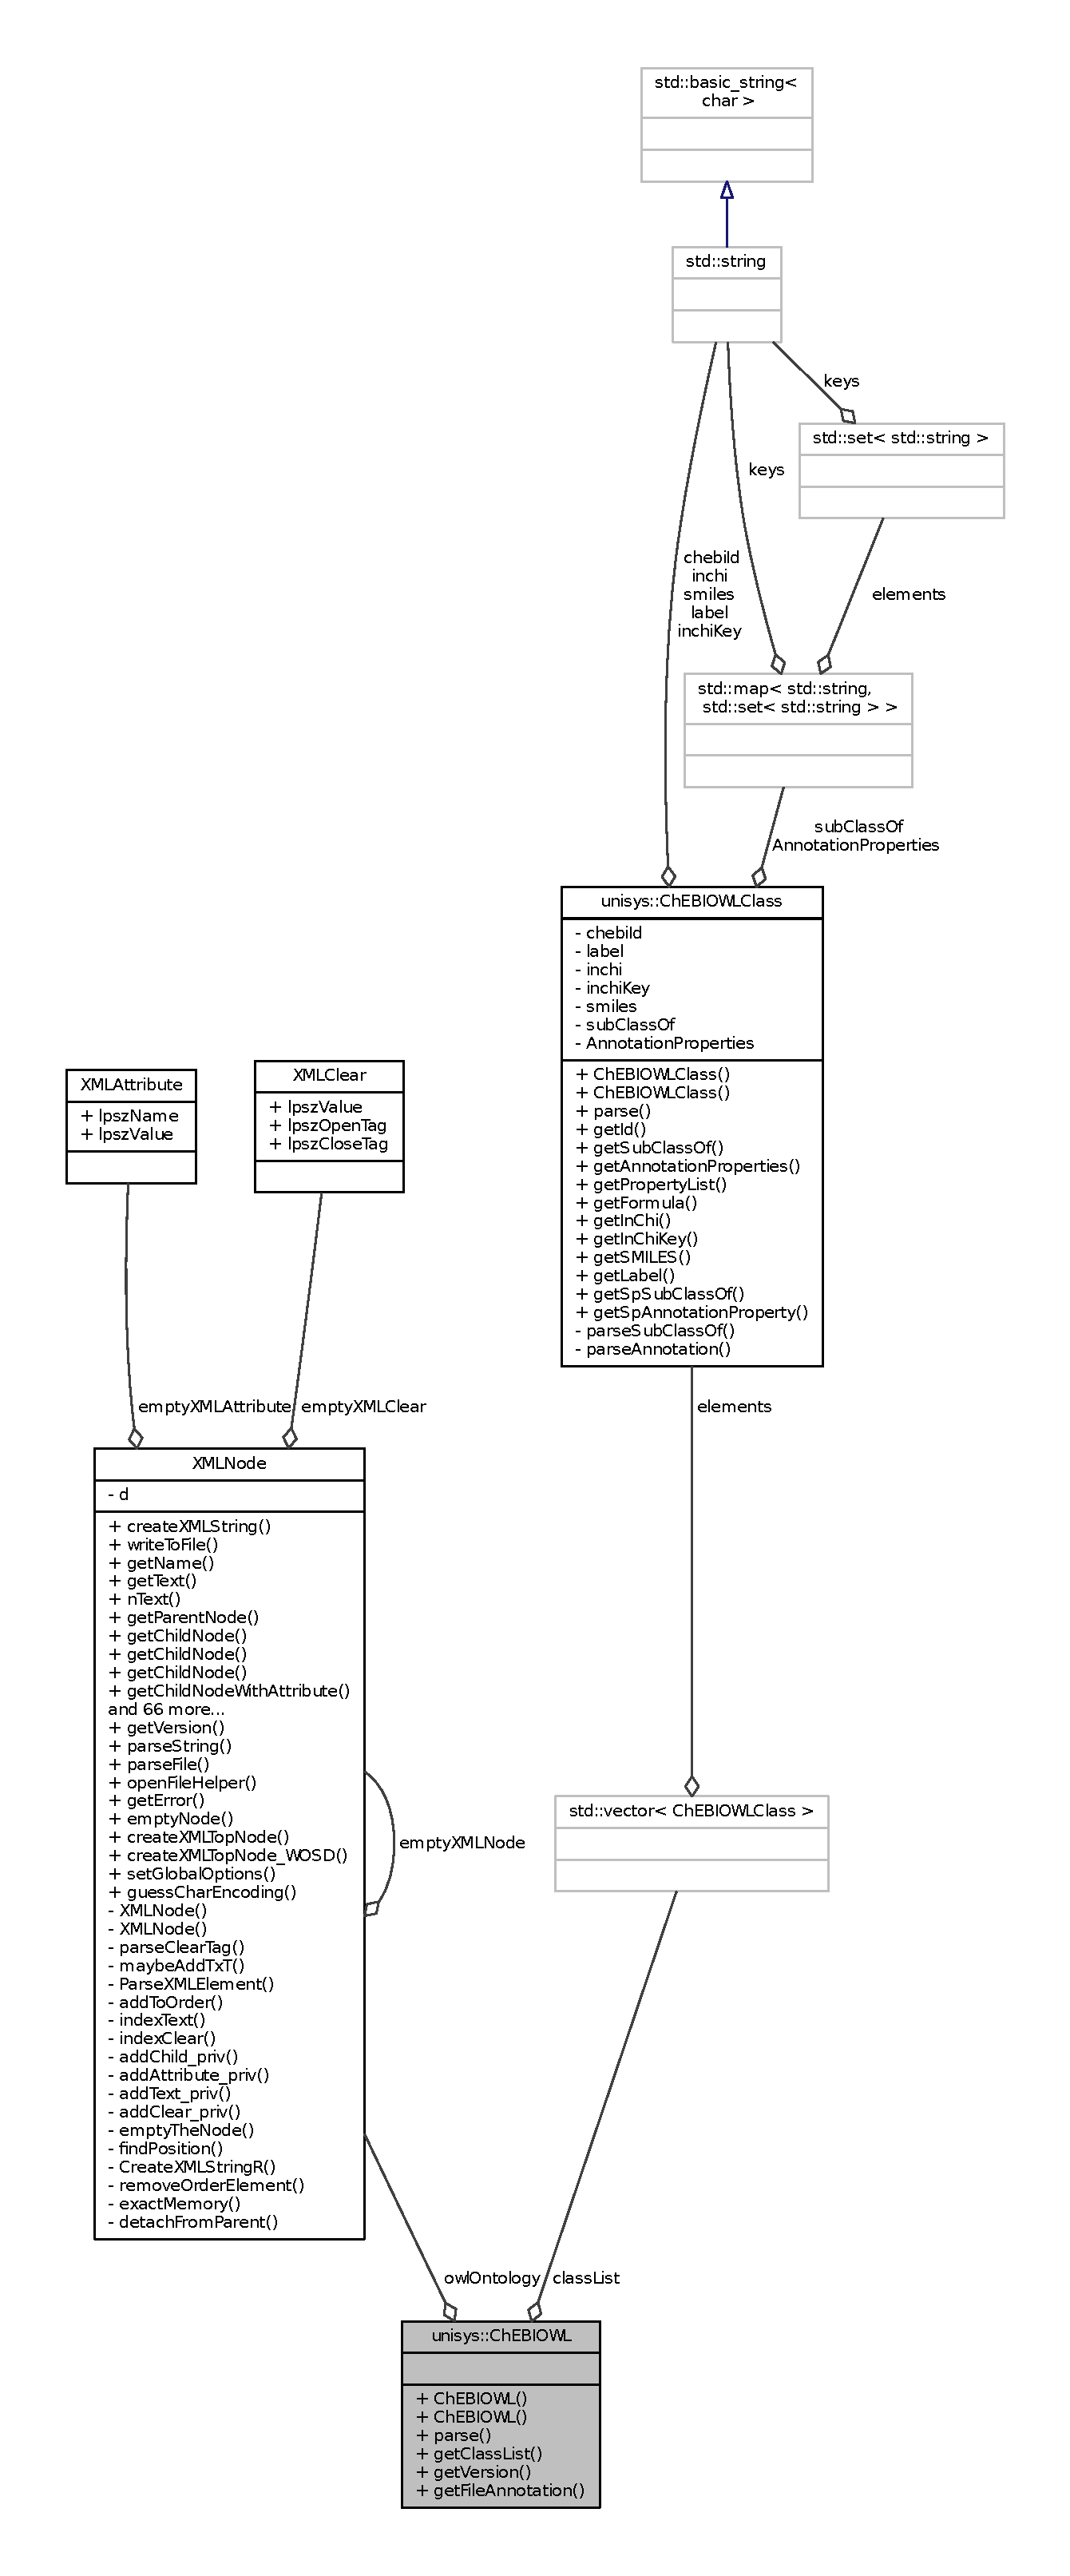
\includegraphics[height=550pt]{classunisys_1_1ChEBIOWL__coll__graph}
\end{center}
\end{figure}
\subsection*{Public Member Functions}
\begin{DoxyCompactItemize}
\item 
\hyperlink{classunisys_1_1ChEBIOWL_a27532c1116f67a40537697be2fd43677}{Ch\-E\-B\-I\-O\-W\-L} ()
\item 
\hyperlink{classunisys_1_1ChEBIOWL_aa1f70f82dbb1b9657e32d6864bfb5f97}{Ch\-E\-B\-I\-O\-W\-L} (std\-::string const \&filename)
\item 
void \hyperlink{classunisys_1_1ChEBIOWL_a83d26bbca0b2c067cbc27f919da5a6a7}{parse} (std\-::string const \&filename)
\item 
std\-::vector$<$ \hyperlink{classunisys_1_1ChEBIOWLClass}{Ch\-E\-B\-I\-O\-W\-L\-Class} $>$ \hyperlink{classunisys_1_1ChEBIOWL_abed6a43a962a98659d28fb9a46232254}{get\-Class\-List} () const 
\item 
std\-::string \hyperlink{classunisys_1_1ChEBIOWL_a381f8bd0263b190157dd586c481083d0}{get\-Version} () const 
\item 
\hyperlink{structXMLNode}{X\-M\-L\-Node} \hyperlink{classunisys_1_1ChEBIOWL_a59e06150bc5b433fdb14e55b1ca95e16}{get\-File\-Annotation} () const 
\end{DoxyCompactItemize}
\subsection*{Private Attributes}
\begin{DoxyCompactItemize}
\item 
\hyperlink{structXMLNode}{X\-M\-L\-Node} \hyperlink{classunisys_1_1ChEBIOWL_af8b35beb7f297b7314a82c011bbb5af8}{owl\-Ontology}
\begin{DoxyCompactList}\small\item\em \hyperlink{classunisys_1_1Ontology}{Ontology} tag with file information. \end{DoxyCompactList}\item 
std\-::vector$<$ \hyperlink{classunisys_1_1ChEBIOWLClass}{Ch\-E\-B\-I\-O\-W\-L\-Class} $>$ \hyperlink{classunisys_1_1ChEBIOWL_a86e75569a9a2110ca09bda3c9e2bcb37}{class\-List}
\begin{DoxyCompactList}\small\item\em vector of \hyperlink{classunisys_1_1ChEBIOWLClass}{Ch\-E\-B\-I\-O\-W\-L\-Class} \end{DoxyCompactList}\end{DoxyCompactItemize}


\subsection{Detailed Description}
Used to parse Ch\-E\-B\-I O\-W\-L format. 

some description. 

\subsection{Constructor \& Destructor Documentation}
\hypertarget{classunisys_1_1ChEBIOWL_a27532c1116f67a40537697be2fd43677}{\index{unisys\-::\-Ch\-E\-B\-I\-O\-W\-L@{unisys\-::\-Ch\-E\-B\-I\-O\-W\-L}!Ch\-E\-B\-I\-O\-W\-L@{Ch\-E\-B\-I\-O\-W\-L}}
\index{Ch\-E\-B\-I\-O\-W\-L@{Ch\-E\-B\-I\-O\-W\-L}!unisys::ChEBIOWL@{unisys\-::\-Ch\-E\-B\-I\-O\-W\-L}}
\subsubsection[{Ch\-E\-B\-I\-O\-W\-L}]{\setlength{\rightskip}{0pt plus 5cm}unisys\-::\-Ch\-E\-B\-I\-O\-W\-L\-::\-Ch\-E\-B\-I\-O\-W\-L (
\begin{DoxyParamCaption}
{}
\end{DoxyParamCaption}
)}}\label{classunisys_1_1ChEBIOWL_a27532c1116f67a40537697be2fd43677}
\hypertarget{classunisys_1_1ChEBIOWL_aa1f70f82dbb1b9657e32d6864bfb5f97}{\index{unisys\-::\-Ch\-E\-B\-I\-O\-W\-L@{unisys\-::\-Ch\-E\-B\-I\-O\-W\-L}!Ch\-E\-B\-I\-O\-W\-L@{Ch\-E\-B\-I\-O\-W\-L}}
\index{Ch\-E\-B\-I\-O\-W\-L@{Ch\-E\-B\-I\-O\-W\-L}!unisys::ChEBIOWL@{unisys\-::\-Ch\-E\-B\-I\-O\-W\-L}}
\subsubsection[{Ch\-E\-B\-I\-O\-W\-L}]{\setlength{\rightskip}{0pt plus 5cm}unisys\-::\-Ch\-E\-B\-I\-O\-W\-L\-::\-Ch\-E\-B\-I\-O\-W\-L (
\begin{DoxyParamCaption}
\item[{std\-::string const \&}]{filename}
\end{DoxyParamCaption}
)}}\label{classunisys_1_1ChEBIOWL_aa1f70f82dbb1b9657e32d6864bfb5f97}


\subsection{Member Function Documentation}
\hypertarget{classunisys_1_1ChEBIOWL_abed6a43a962a98659d28fb9a46232254}{\index{unisys\-::\-Ch\-E\-B\-I\-O\-W\-L@{unisys\-::\-Ch\-E\-B\-I\-O\-W\-L}!get\-Class\-List@{get\-Class\-List}}
\index{get\-Class\-List@{get\-Class\-List}!unisys::ChEBIOWL@{unisys\-::\-Ch\-E\-B\-I\-O\-W\-L}}
\subsubsection[{get\-Class\-List}]{\setlength{\rightskip}{0pt plus 5cm}std\-::vector$<${\bf Ch\-E\-B\-I\-O\-W\-L\-Class}$>$ unisys\-::\-Ch\-E\-B\-I\-O\-W\-L\-::get\-Class\-List (
\begin{DoxyParamCaption}
{}
\end{DoxyParamCaption}
) const}}\label{classunisys_1_1ChEBIOWL_abed6a43a962a98659d28fb9a46232254}
\hypertarget{classunisys_1_1ChEBIOWL_a59e06150bc5b433fdb14e55b1ca95e16}{\index{unisys\-::\-Ch\-E\-B\-I\-O\-W\-L@{unisys\-::\-Ch\-E\-B\-I\-O\-W\-L}!get\-File\-Annotation@{get\-File\-Annotation}}
\index{get\-File\-Annotation@{get\-File\-Annotation}!unisys::ChEBIOWL@{unisys\-::\-Ch\-E\-B\-I\-O\-W\-L}}
\subsubsection[{get\-File\-Annotation}]{\setlength{\rightskip}{0pt plus 5cm}{\bf X\-M\-L\-Node} unisys\-::\-Ch\-E\-B\-I\-O\-W\-L\-::get\-File\-Annotation (
\begin{DoxyParamCaption}
{}
\end{DoxyParamCaption}
) const}}\label{classunisys_1_1ChEBIOWL_a59e06150bc5b433fdb14e55b1ca95e16}
\hypertarget{classunisys_1_1ChEBIOWL_a381f8bd0263b190157dd586c481083d0}{\index{unisys\-::\-Ch\-E\-B\-I\-O\-W\-L@{unisys\-::\-Ch\-E\-B\-I\-O\-W\-L}!get\-Version@{get\-Version}}
\index{get\-Version@{get\-Version}!unisys::ChEBIOWL@{unisys\-::\-Ch\-E\-B\-I\-O\-W\-L}}
\subsubsection[{get\-Version}]{\setlength{\rightskip}{0pt plus 5cm}std\-::string unisys\-::\-Ch\-E\-B\-I\-O\-W\-L\-::get\-Version (
\begin{DoxyParamCaption}
{}
\end{DoxyParamCaption}
) const}}\label{classunisys_1_1ChEBIOWL_a381f8bd0263b190157dd586c481083d0}
\hypertarget{classunisys_1_1ChEBIOWL_a83d26bbca0b2c067cbc27f919da5a6a7}{\index{unisys\-::\-Ch\-E\-B\-I\-O\-W\-L@{unisys\-::\-Ch\-E\-B\-I\-O\-W\-L}!parse@{parse}}
\index{parse@{parse}!unisys::ChEBIOWL@{unisys\-::\-Ch\-E\-B\-I\-O\-W\-L}}
\subsubsection[{parse}]{\setlength{\rightskip}{0pt plus 5cm}void unisys\-::\-Ch\-E\-B\-I\-O\-W\-L\-::parse (
\begin{DoxyParamCaption}
\item[{std\-::string const \&}]{filename}
\end{DoxyParamCaption}
)}}\label{classunisys_1_1ChEBIOWL_a83d26bbca0b2c067cbc27f919da5a6a7}


\subsection{Member Data Documentation}
\hypertarget{classunisys_1_1ChEBIOWL_a86e75569a9a2110ca09bda3c9e2bcb37}{\index{unisys\-::\-Ch\-E\-B\-I\-O\-W\-L@{unisys\-::\-Ch\-E\-B\-I\-O\-W\-L}!class\-List@{class\-List}}
\index{class\-List@{class\-List}!unisys::ChEBIOWL@{unisys\-::\-Ch\-E\-B\-I\-O\-W\-L}}
\subsubsection[{class\-List}]{\setlength{\rightskip}{0pt plus 5cm}std\-::vector$<${\bf Ch\-E\-B\-I\-O\-W\-L\-Class}$>$ unisys\-::\-Ch\-E\-B\-I\-O\-W\-L\-::class\-List\hspace{0.3cm}{\ttfamily [private]}}}\label{classunisys_1_1ChEBIOWL_a86e75569a9a2110ca09bda3c9e2bcb37}


vector of \hyperlink{classunisys_1_1ChEBIOWLClass}{Ch\-E\-B\-I\-O\-W\-L\-Class} 

\hypertarget{classunisys_1_1ChEBIOWL_af8b35beb7f297b7314a82c011bbb5af8}{\index{unisys\-::\-Ch\-E\-B\-I\-O\-W\-L@{unisys\-::\-Ch\-E\-B\-I\-O\-W\-L}!owl\-Ontology@{owl\-Ontology}}
\index{owl\-Ontology@{owl\-Ontology}!unisys::ChEBIOWL@{unisys\-::\-Ch\-E\-B\-I\-O\-W\-L}}
\subsubsection[{owl\-Ontology}]{\setlength{\rightskip}{0pt plus 5cm}{\bf X\-M\-L\-Node} unisys\-::\-Ch\-E\-B\-I\-O\-W\-L\-::owl\-Ontology\hspace{0.3cm}{\ttfamily [private]}}}\label{classunisys_1_1ChEBIOWL_af8b35beb7f297b7314a82c011bbb5af8}


\hyperlink{classunisys_1_1Ontology}{Ontology} tag with file information. 



The documentation for this class was generated from the following file\-:\begin{DoxyCompactItemize}
\item 
\hyperlink{chebiowl_8h}{chebiowl.\-h}\end{DoxyCompactItemize}

\hypertarget{classunisys_1_1ChEBIOWLClass}{\section{unisys\-:\-:Ch\-E\-B\-I\-O\-W\-L\-Class Class Reference}
\label{classunisys_1_1ChEBIOWLClass}\index{unisys\-::\-Ch\-E\-B\-I\-O\-W\-L\-Class@{unisys\-::\-Ch\-E\-B\-I\-O\-W\-L\-Class}}
}


To handle owl\-:class tag of Ch\-E\-B\-I O\-W\-L format.  




{\ttfamily \#include $<$chebiowl.\-h$>$}



Collaboration diagram for unisys\-:\-:Ch\-E\-B\-I\-O\-W\-L\-Class\-:
\nopagebreak
\begin{figure}[H]
\begin{center}
\leavevmode
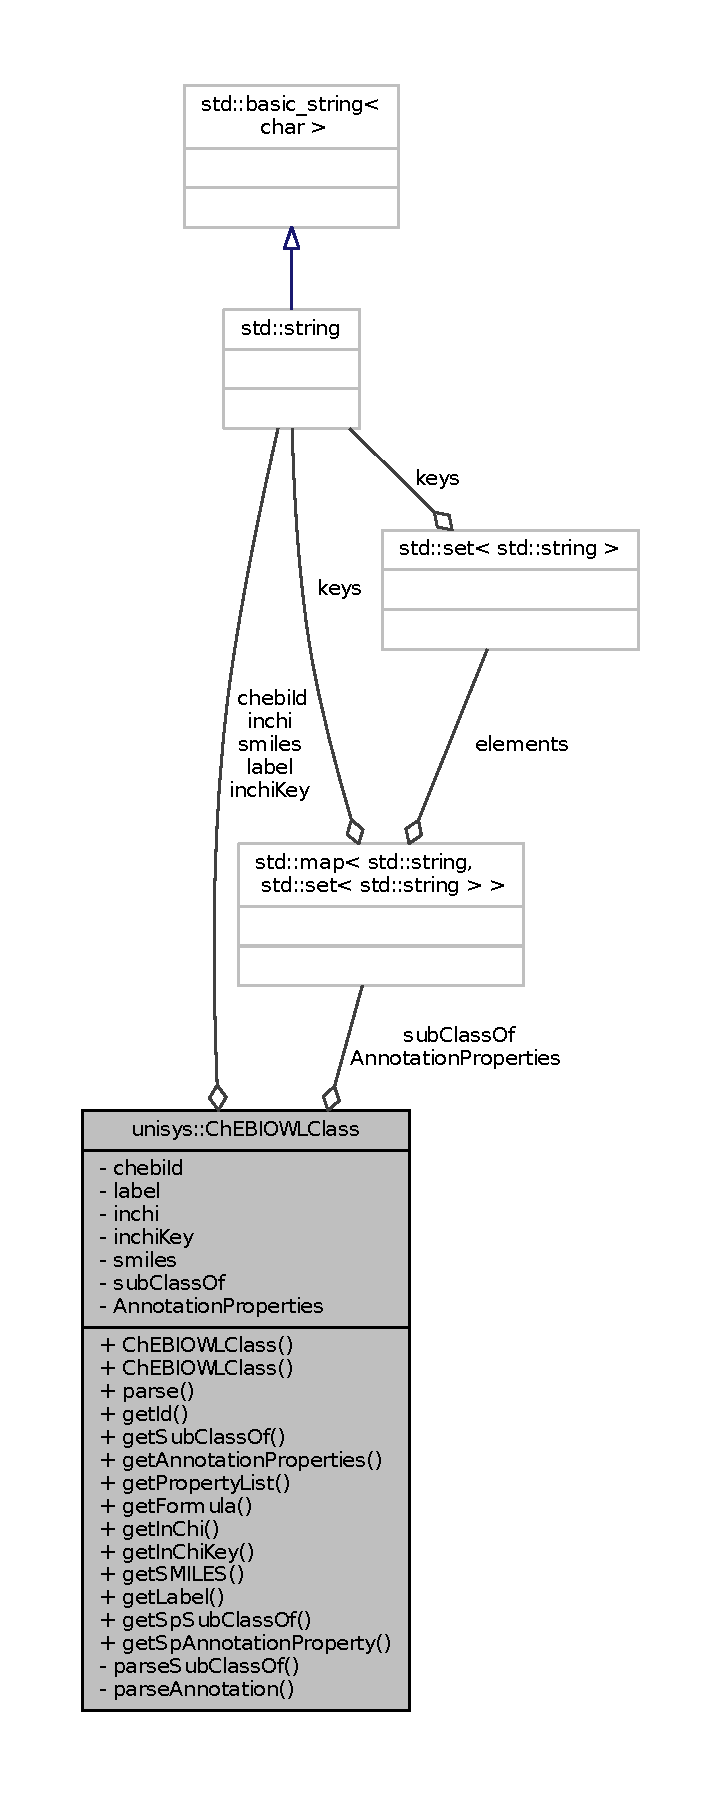
\includegraphics[height=550pt]{classunisys_1_1ChEBIOWLClass__coll__graph}
\end{center}
\end{figure}
\subsection*{Public Member Functions}
\begin{DoxyCompactItemize}
\item 
\hyperlink{classunisys_1_1ChEBIOWLClass_a2399546f521a8944c9d2d684d34cffbb}{Ch\-E\-B\-I\-O\-W\-L\-Class} ()
\item 
\hyperlink{classunisys_1_1ChEBIOWLClass_a286dbb327267e654ac903076ace09ebf}{Ch\-E\-B\-I\-O\-W\-L\-Class} (\hyperlink{structXMLNode}{X\-M\-L\-Node} xml)
\item 
void \hyperlink{classunisys_1_1ChEBIOWLClass_a923d1d7e6c6db3cf16f6fa0d361354e6}{parse} (\hyperlink{structXMLNode}{X\-M\-L\-Node} xml)  throw (\-Parsing\-Error)
\item 
std\-::string \hyperlink{classunisys_1_1ChEBIOWLClass_a065642342c1d6128eed047eb0ac2cc86}{get\-Id} () const 
\item 
std\-::map$<$ std\-::string, \\*
std\-::set$<$ std\-::string $>$ $>$ \hyperlink{classunisys_1_1ChEBIOWLClass_aee6d27a23c8d37f32e615c092b21bc6f}{get\-Sub\-Class\-Of} () const 
\item 
std\-::map$<$ std\-::string, \\*
std\-::set$<$ std\-::string $>$ $>$ \hyperlink{classunisys_1_1ChEBIOWLClass_a4f26e034a7e67b315b849214d339d518}{get\-Annotation\-Properties} () const 
\item 
std\-::set$<$ std\-::string $>$ \hyperlink{classunisys_1_1ChEBIOWLClass_af58a3d6397491f2ca151ddde60fc87b3}{get\-Property\-List} () const 
\item 
std\-::string \hyperlink{classunisys_1_1ChEBIOWLClass_aca905897ba7ec051f58d8678c0212443}{get\-Formula} () const 
\item 
std\-::string \hyperlink{classunisys_1_1ChEBIOWLClass_a99a66fa3cfd603164048154e6c69d81a}{get\-In\-Chi} () const 
\item 
std\-::string \hyperlink{classunisys_1_1ChEBIOWLClass_acaae86d1b5cf33a684d7ffbdc0bd32d8}{get\-In\-Chi\-Key} () const 
\item 
std\-::string \hyperlink{classunisys_1_1ChEBIOWLClass_a43fe054e370a5d6e451c85826b089eb1}{get\-S\-M\-I\-L\-E\-S} () const 
\item 
std\-::string \hyperlink{classunisys_1_1ChEBIOWLClass_a50cb32b74994a3a8313bd3a8ed1f0f6d}{get\-Label} () const 
\item 
std\-::set$<$ std\-::string $>$ \hyperlink{classunisys_1_1ChEBIOWLClass_af0bcc628140659b151e773eba2a9c1fb}{get\-Sp\-Sub\-Class\-Of} (std\-::string const \&sub\-Class\-Type) const 
\item 
std\-::set$<$ std\-::string $>$ \hyperlink{classunisys_1_1ChEBIOWLClass_a7673a9020ac603b41004bcb4a743d568}{get\-Sp\-Annotation\-Property} (std\-::string const \&properties\-Name) const 
\end{DoxyCompactItemize}
\subsection*{Private Member Functions}
\begin{DoxyCompactItemize}
\item 
void \hyperlink{classunisys_1_1ChEBIOWLClass_ae682fc16d656c5970f82a66f061950dc}{parse\-Sub\-Class\-Of} (\hyperlink{structXMLNode}{X\-M\-L\-Node} xml)  throw (\-Parsing\-Error)
\begin{DoxyCompactList}\small\item\em Parsing Sub\-Class\-Of tag. \end{DoxyCompactList}\item 
void \hyperlink{classunisys_1_1ChEBIOWLClass_af23bf20388d5b25b4312fe2bedf6c3d6}{parse\-Annotation} (\hyperlink{structXMLNode}{X\-M\-L\-Node} xml)  throw (\-Parsing\-Error)
\begin{DoxyCompactList}\small\item\em Parsing \hyperlink{classunisys_1_1Annotation}{Annotation} tag. \end{DoxyCompactList}\end{DoxyCompactItemize}
\subsection*{Private Attributes}
\begin{DoxyCompactItemize}
\item 
std\-::string \hyperlink{classunisys_1_1ChEBIOWLClass_ab117174852af50b086c9baf28647be85}{chebi\-Id}
\begin{DoxyCompactList}\small\item\em Ch\-E\-B\-I I\-D in /\-C\-H\-E\-B\-I\-:+/ format. \end{DoxyCompactList}\item 
std\-::string \hyperlink{classunisys_1_1ChEBIOWLClass_a5069859deb537ea460525e98d277397c}{label}
\begin{DoxyCompactList}\small\item\em Name of Ch\-E\-B\-I entity. \end{DoxyCompactList}\item 
std\-::string \hyperlink{classunisys_1_1ChEBIOWLClass_a46b2c202643987ce0d4e3a105e117822}{inchi}
\item 
std\-::string \hyperlink{classunisys_1_1ChEBIOWLClass_af64b976dc7f141a4935898fcb470cefb}{inchi\-Key}
\item 
std\-::string \hyperlink{classunisys_1_1ChEBIOWLClass_ad36fc8f28f36623552de31e77095e570}{smiles}
\item 
std\-::map$<$ std\-::string, \\*
std\-::set$<$ std\-::string $>$ $>$ \hyperlink{classunisys_1_1ChEBIOWLClass_afac1eca0e61d1adcebd6d1feda765a63}{sub\-Class\-Of}
\begin{DoxyCompactList}\small\item\em Relationship tag. \end{DoxyCompactList}\item 
std\-::map$<$ std\-::string, \\*
std\-::set$<$ std\-::string $>$ $>$ \hyperlink{classunisys_1_1ChEBIOWLClass_a4f4fec0580d988965e1ab42c8aecbb59}{Annotation\-Properties}
\begin{DoxyCompactList}\small\item\em \hyperlink{classunisys_1_1Annotation}{Annotation} tag except In\-Chi, In\-Chi\-Key and S\-M\-I\-L\-E\-S. \end{DoxyCompactList}\end{DoxyCompactItemize}


\subsection{Detailed Description}
To handle owl\-:class tag of Ch\-E\-B\-I O\-W\-L format. 

some description. 

\subsection{Constructor \& Destructor Documentation}
\hypertarget{classunisys_1_1ChEBIOWLClass_a2399546f521a8944c9d2d684d34cffbb}{\index{unisys\-::\-Ch\-E\-B\-I\-O\-W\-L\-Class@{unisys\-::\-Ch\-E\-B\-I\-O\-W\-L\-Class}!Ch\-E\-B\-I\-O\-W\-L\-Class@{Ch\-E\-B\-I\-O\-W\-L\-Class}}
\index{Ch\-E\-B\-I\-O\-W\-L\-Class@{Ch\-E\-B\-I\-O\-W\-L\-Class}!unisys::ChEBIOWLClass@{unisys\-::\-Ch\-E\-B\-I\-O\-W\-L\-Class}}
\subsubsection[{Ch\-E\-B\-I\-O\-W\-L\-Class}]{\setlength{\rightskip}{0pt plus 5cm}unisys\-::\-Ch\-E\-B\-I\-O\-W\-L\-Class\-::\-Ch\-E\-B\-I\-O\-W\-L\-Class (
\begin{DoxyParamCaption}
{}
\end{DoxyParamCaption}
)}}\label{classunisys_1_1ChEBIOWLClass_a2399546f521a8944c9d2d684d34cffbb}
\hypertarget{classunisys_1_1ChEBIOWLClass_a286dbb327267e654ac903076ace09ebf}{\index{unisys\-::\-Ch\-E\-B\-I\-O\-W\-L\-Class@{unisys\-::\-Ch\-E\-B\-I\-O\-W\-L\-Class}!Ch\-E\-B\-I\-O\-W\-L\-Class@{Ch\-E\-B\-I\-O\-W\-L\-Class}}
\index{Ch\-E\-B\-I\-O\-W\-L\-Class@{Ch\-E\-B\-I\-O\-W\-L\-Class}!unisys::ChEBIOWLClass@{unisys\-::\-Ch\-E\-B\-I\-O\-W\-L\-Class}}
\subsubsection[{Ch\-E\-B\-I\-O\-W\-L\-Class}]{\setlength{\rightskip}{0pt plus 5cm}unisys\-::\-Ch\-E\-B\-I\-O\-W\-L\-Class\-::\-Ch\-E\-B\-I\-O\-W\-L\-Class (
\begin{DoxyParamCaption}
\item[{{\bf X\-M\-L\-Node}}]{xml}
\end{DoxyParamCaption}
)}}\label{classunisys_1_1ChEBIOWLClass_a286dbb327267e654ac903076ace09ebf}


\subsection{Member Function Documentation}
\hypertarget{classunisys_1_1ChEBIOWLClass_a4f26e034a7e67b315b849214d339d518}{\index{unisys\-::\-Ch\-E\-B\-I\-O\-W\-L\-Class@{unisys\-::\-Ch\-E\-B\-I\-O\-W\-L\-Class}!get\-Annotation\-Properties@{get\-Annotation\-Properties}}
\index{get\-Annotation\-Properties@{get\-Annotation\-Properties}!unisys::ChEBIOWLClass@{unisys\-::\-Ch\-E\-B\-I\-O\-W\-L\-Class}}
\subsubsection[{get\-Annotation\-Properties}]{\setlength{\rightskip}{0pt plus 5cm}std\-::map$<$std\-::string, std\-::set$<$std\-::string$>$ $>$ unisys\-::\-Ch\-E\-B\-I\-O\-W\-L\-Class\-::get\-Annotation\-Properties (
\begin{DoxyParamCaption}
{}
\end{DoxyParamCaption}
) const}}\label{classunisys_1_1ChEBIOWLClass_a4f26e034a7e67b315b849214d339d518}
\hypertarget{classunisys_1_1ChEBIOWLClass_aca905897ba7ec051f58d8678c0212443}{\index{unisys\-::\-Ch\-E\-B\-I\-O\-W\-L\-Class@{unisys\-::\-Ch\-E\-B\-I\-O\-W\-L\-Class}!get\-Formula@{get\-Formula}}
\index{get\-Formula@{get\-Formula}!unisys::ChEBIOWLClass@{unisys\-::\-Ch\-E\-B\-I\-O\-W\-L\-Class}}
\subsubsection[{get\-Formula}]{\setlength{\rightskip}{0pt plus 5cm}std\-::string unisys\-::\-Ch\-E\-B\-I\-O\-W\-L\-Class\-::get\-Formula (
\begin{DoxyParamCaption}
{}
\end{DoxyParamCaption}
) const}}\label{classunisys_1_1ChEBIOWLClass_aca905897ba7ec051f58d8678c0212443}
\hypertarget{classunisys_1_1ChEBIOWLClass_a065642342c1d6128eed047eb0ac2cc86}{\index{unisys\-::\-Ch\-E\-B\-I\-O\-W\-L\-Class@{unisys\-::\-Ch\-E\-B\-I\-O\-W\-L\-Class}!get\-Id@{get\-Id}}
\index{get\-Id@{get\-Id}!unisys::ChEBIOWLClass@{unisys\-::\-Ch\-E\-B\-I\-O\-W\-L\-Class}}
\subsubsection[{get\-Id}]{\setlength{\rightskip}{0pt plus 5cm}std\-::string unisys\-::\-Ch\-E\-B\-I\-O\-W\-L\-Class\-::get\-Id (
\begin{DoxyParamCaption}
{}
\end{DoxyParamCaption}
) const}}\label{classunisys_1_1ChEBIOWLClass_a065642342c1d6128eed047eb0ac2cc86}
\hypertarget{classunisys_1_1ChEBIOWLClass_a99a66fa3cfd603164048154e6c69d81a}{\index{unisys\-::\-Ch\-E\-B\-I\-O\-W\-L\-Class@{unisys\-::\-Ch\-E\-B\-I\-O\-W\-L\-Class}!get\-In\-Chi@{get\-In\-Chi}}
\index{get\-In\-Chi@{get\-In\-Chi}!unisys::ChEBIOWLClass@{unisys\-::\-Ch\-E\-B\-I\-O\-W\-L\-Class}}
\subsubsection[{get\-In\-Chi}]{\setlength{\rightskip}{0pt plus 5cm}std\-::string unisys\-::\-Ch\-E\-B\-I\-O\-W\-L\-Class\-::get\-In\-Chi (
\begin{DoxyParamCaption}
{}
\end{DoxyParamCaption}
) const}}\label{classunisys_1_1ChEBIOWLClass_a99a66fa3cfd603164048154e6c69d81a}
\hypertarget{classunisys_1_1ChEBIOWLClass_acaae86d1b5cf33a684d7ffbdc0bd32d8}{\index{unisys\-::\-Ch\-E\-B\-I\-O\-W\-L\-Class@{unisys\-::\-Ch\-E\-B\-I\-O\-W\-L\-Class}!get\-In\-Chi\-Key@{get\-In\-Chi\-Key}}
\index{get\-In\-Chi\-Key@{get\-In\-Chi\-Key}!unisys::ChEBIOWLClass@{unisys\-::\-Ch\-E\-B\-I\-O\-W\-L\-Class}}
\subsubsection[{get\-In\-Chi\-Key}]{\setlength{\rightskip}{0pt plus 5cm}std\-::string unisys\-::\-Ch\-E\-B\-I\-O\-W\-L\-Class\-::get\-In\-Chi\-Key (
\begin{DoxyParamCaption}
{}
\end{DoxyParamCaption}
) const}}\label{classunisys_1_1ChEBIOWLClass_acaae86d1b5cf33a684d7ffbdc0bd32d8}
\hypertarget{classunisys_1_1ChEBIOWLClass_a50cb32b74994a3a8313bd3a8ed1f0f6d}{\index{unisys\-::\-Ch\-E\-B\-I\-O\-W\-L\-Class@{unisys\-::\-Ch\-E\-B\-I\-O\-W\-L\-Class}!get\-Label@{get\-Label}}
\index{get\-Label@{get\-Label}!unisys::ChEBIOWLClass@{unisys\-::\-Ch\-E\-B\-I\-O\-W\-L\-Class}}
\subsubsection[{get\-Label}]{\setlength{\rightskip}{0pt plus 5cm}std\-::string unisys\-::\-Ch\-E\-B\-I\-O\-W\-L\-Class\-::get\-Label (
\begin{DoxyParamCaption}
{}
\end{DoxyParamCaption}
) const}}\label{classunisys_1_1ChEBIOWLClass_a50cb32b74994a3a8313bd3a8ed1f0f6d}
\hypertarget{classunisys_1_1ChEBIOWLClass_af58a3d6397491f2ca151ddde60fc87b3}{\index{unisys\-::\-Ch\-E\-B\-I\-O\-W\-L\-Class@{unisys\-::\-Ch\-E\-B\-I\-O\-W\-L\-Class}!get\-Property\-List@{get\-Property\-List}}
\index{get\-Property\-List@{get\-Property\-List}!unisys::ChEBIOWLClass@{unisys\-::\-Ch\-E\-B\-I\-O\-W\-L\-Class}}
\subsubsection[{get\-Property\-List}]{\setlength{\rightskip}{0pt plus 5cm}std\-::set$<$std\-::string$>$ unisys\-::\-Ch\-E\-B\-I\-O\-W\-L\-Class\-::get\-Property\-List (
\begin{DoxyParamCaption}
{}
\end{DoxyParamCaption}
) const}}\label{classunisys_1_1ChEBIOWLClass_af58a3d6397491f2ca151ddde60fc87b3}
\hypertarget{classunisys_1_1ChEBIOWLClass_a43fe054e370a5d6e451c85826b089eb1}{\index{unisys\-::\-Ch\-E\-B\-I\-O\-W\-L\-Class@{unisys\-::\-Ch\-E\-B\-I\-O\-W\-L\-Class}!get\-S\-M\-I\-L\-E\-S@{get\-S\-M\-I\-L\-E\-S}}
\index{get\-S\-M\-I\-L\-E\-S@{get\-S\-M\-I\-L\-E\-S}!unisys::ChEBIOWLClass@{unisys\-::\-Ch\-E\-B\-I\-O\-W\-L\-Class}}
\subsubsection[{get\-S\-M\-I\-L\-E\-S}]{\setlength{\rightskip}{0pt plus 5cm}std\-::string unisys\-::\-Ch\-E\-B\-I\-O\-W\-L\-Class\-::get\-S\-M\-I\-L\-E\-S (
\begin{DoxyParamCaption}
{}
\end{DoxyParamCaption}
) const}}\label{classunisys_1_1ChEBIOWLClass_a43fe054e370a5d6e451c85826b089eb1}
\hypertarget{classunisys_1_1ChEBIOWLClass_a7673a9020ac603b41004bcb4a743d568}{\index{unisys\-::\-Ch\-E\-B\-I\-O\-W\-L\-Class@{unisys\-::\-Ch\-E\-B\-I\-O\-W\-L\-Class}!get\-Sp\-Annotation\-Property@{get\-Sp\-Annotation\-Property}}
\index{get\-Sp\-Annotation\-Property@{get\-Sp\-Annotation\-Property}!unisys::ChEBIOWLClass@{unisys\-::\-Ch\-E\-B\-I\-O\-W\-L\-Class}}
\subsubsection[{get\-Sp\-Annotation\-Property}]{\setlength{\rightskip}{0pt plus 5cm}std\-::set$<$std\-::string$>$ unisys\-::\-Ch\-E\-B\-I\-O\-W\-L\-Class\-::get\-Sp\-Annotation\-Property (
\begin{DoxyParamCaption}
\item[{std\-::string const \&}]{properties\-Name}
\end{DoxyParamCaption}
) const}}\label{classunisys_1_1ChEBIOWLClass_a7673a9020ac603b41004bcb4a743d568}
\hypertarget{classunisys_1_1ChEBIOWLClass_af0bcc628140659b151e773eba2a9c1fb}{\index{unisys\-::\-Ch\-E\-B\-I\-O\-W\-L\-Class@{unisys\-::\-Ch\-E\-B\-I\-O\-W\-L\-Class}!get\-Sp\-Sub\-Class\-Of@{get\-Sp\-Sub\-Class\-Of}}
\index{get\-Sp\-Sub\-Class\-Of@{get\-Sp\-Sub\-Class\-Of}!unisys::ChEBIOWLClass@{unisys\-::\-Ch\-E\-B\-I\-O\-W\-L\-Class}}
\subsubsection[{get\-Sp\-Sub\-Class\-Of}]{\setlength{\rightskip}{0pt plus 5cm}std\-::set$<$std\-::string$>$ unisys\-::\-Ch\-E\-B\-I\-O\-W\-L\-Class\-::get\-Sp\-Sub\-Class\-Of (
\begin{DoxyParamCaption}
\item[{std\-::string const \&}]{sub\-Class\-Type}
\end{DoxyParamCaption}
) const}}\label{classunisys_1_1ChEBIOWLClass_af0bcc628140659b151e773eba2a9c1fb}
\hypertarget{classunisys_1_1ChEBIOWLClass_aee6d27a23c8d37f32e615c092b21bc6f}{\index{unisys\-::\-Ch\-E\-B\-I\-O\-W\-L\-Class@{unisys\-::\-Ch\-E\-B\-I\-O\-W\-L\-Class}!get\-Sub\-Class\-Of@{get\-Sub\-Class\-Of}}
\index{get\-Sub\-Class\-Of@{get\-Sub\-Class\-Of}!unisys::ChEBIOWLClass@{unisys\-::\-Ch\-E\-B\-I\-O\-W\-L\-Class}}
\subsubsection[{get\-Sub\-Class\-Of}]{\setlength{\rightskip}{0pt plus 5cm}std\-::map$<$std\-::string, std\-::set$<$std\-::string$>$ $>$ unisys\-::\-Ch\-E\-B\-I\-O\-W\-L\-Class\-::get\-Sub\-Class\-Of (
\begin{DoxyParamCaption}
{}
\end{DoxyParamCaption}
) const}}\label{classunisys_1_1ChEBIOWLClass_aee6d27a23c8d37f32e615c092b21bc6f}
\hypertarget{classunisys_1_1ChEBIOWLClass_a923d1d7e6c6db3cf16f6fa0d361354e6}{\index{unisys\-::\-Ch\-E\-B\-I\-O\-W\-L\-Class@{unisys\-::\-Ch\-E\-B\-I\-O\-W\-L\-Class}!parse@{parse}}
\index{parse@{parse}!unisys::ChEBIOWLClass@{unisys\-::\-Ch\-E\-B\-I\-O\-W\-L\-Class}}
\subsubsection[{parse}]{\setlength{\rightskip}{0pt plus 5cm}void unisys\-::\-Ch\-E\-B\-I\-O\-W\-L\-Class\-::parse (
\begin{DoxyParamCaption}
\item[{{\bf X\-M\-L\-Node}}]{xml}
\end{DoxyParamCaption}
)  throw ({\bf Parsing\-Error})}}\label{classunisys_1_1ChEBIOWLClass_a923d1d7e6c6db3cf16f6fa0d361354e6}
\hypertarget{classunisys_1_1ChEBIOWLClass_af23bf20388d5b25b4312fe2bedf6c3d6}{\index{unisys\-::\-Ch\-E\-B\-I\-O\-W\-L\-Class@{unisys\-::\-Ch\-E\-B\-I\-O\-W\-L\-Class}!parse\-Annotation@{parse\-Annotation}}
\index{parse\-Annotation@{parse\-Annotation}!unisys::ChEBIOWLClass@{unisys\-::\-Ch\-E\-B\-I\-O\-W\-L\-Class}}
\subsubsection[{parse\-Annotation}]{\setlength{\rightskip}{0pt plus 5cm}void unisys\-::\-Ch\-E\-B\-I\-O\-W\-L\-Class\-::parse\-Annotation (
\begin{DoxyParamCaption}
\item[{{\bf X\-M\-L\-Node}}]{xml}
\end{DoxyParamCaption}
)  throw ({\bf Parsing\-Error})\hspace{0.3cm}{\ttfamily [private]}}}\label{classunisys_1_1ChEBIOWLClass_af23bf20388d5b25b4312fe2bedf6c3d6}


Parsing \hyperlink{classunisys_1_1Annotation}{Annotation} tag. 

\hypertarget{classunisys_1_1ChEBIOWLClass_ae682fc16d656c5970f82a66f061950dc}{\index{unisys\-::\-Ch\-E\-B\-I\-O\-W\-L\-Class@{unisys\-::\-Ch\-E\-B\-I\-O\-W\-L\-Class}!parse\-Sub\-Class\-Of@{parse\-Sub\-Class\-Of}}
\index{parse\-Sub\-Class\-Of@{parse\-Sub\-Class\-Of}!unisys::ChEBIOWLClass@{unisys\-::\-Ch\-E\-B\-I\-O\-W\-L\-Class}}
\subsubsection[{parse\-Sub\-Class\-Of}]{\setlength{\rightskip}{0pt plus 5cm}void unisys\-::\-Ch\-E\-B\-I\-O\-W\-L\-Class\-::parse\-Sub\-Class\-Of (
\begin{DoxyParamCaption}
\item[{{\bf X\-M\-L\-Node}}]{xml}
\end{DoxyParamCaption}
)  throw ({\bf Parsing\-Error})\hspace{0.3cm}{\ttfamily [private]}}}\label{classunisys_1_1ChEBIOWLClass_ae682fc16d656c5970f82a66f061950dc}


Parsing Sub\-Class\-Of tag. 



\subsection{Member Data Documentation}
\hypertarget{classunisys_1_1ChEBIOWLClass_a4f4fec0580d988965e1ab42c8aecbb59}{\index{unisys\-::\-Ch\-E\-B\-I\-O\-W\-L\-Class@{unisys\-::\-Ch\-E\-B\-I\-O\-W\-L\-Class}!Annotation\-Properties@{Annotation\-Properties}}
\index{Annotation\-Properties@{Annotation\-Properties}!unisys::ChEBIOWLClass@{unisys\-::\-Ch\-E\-B\-I\-O\-W\-L\-Class}}
\subsubsection[{Annotation\-Properties}]{\setlength{\rightskip}{0pt plus 5cm}std\-::map$<$std\-::string, std\-::set$<$std\-::string$>$ $>$ unisys\-::\-Ch\-E\-B\-I\-O\-W\-L\-Class\-::\-Annotation\-Properties\hspace{0.3cm}{\ttfamily [private]}}}\label{classunisys_1_1ChEBIOWLClass_a4f4fec0580d988965e1ab42c8aecbb59}


\hyperlink{classunisys_1_1Annotation}{Annotation} tag except In\-Chi, In\-Chi\-Key and S\-M\-I\-L\-E\-S. 

\hypertarget{classunisys_1_1ChEBIOWLClass_ab117174852af50b086c9baf28647be85}{\index{unisys\-::\-Ch\-E\-B\-I\-O\-W\-L\-Class@{unisys\-::\-Ch\-E\-B\-I\-O\-W\-L\-Class}!chebi\-Id@{chebi\-Id}}
\index{chebi\-Id@{chebi\-Id}!unisys::ChEBIOWLClass@{unisys\-::\-Ch\-E\-B\-I\-O\-W\-L\-Class}}
\subsubsection[{chebi\-Id}]{\setlength{\rightskip}{0pt plus 5cm}std\-::string unisys\-::\-Ch\-E\-B\-I\-O\-W\-L\-Class\-::chebi\-Id\hspace{0.3cm}{\ttfamily [private]}}}\label{classunisys_1_1ChEBIOWLClass_ab117174852af50b086c9baf28647be85}


Ch\-E\-B\-I I\-D in /\-C\-H\-E\-B\-I\-:+/ format. 

\hypertarget{classunisys_1_1ChEBIOWLClass_a46b2c202643987ce0d4e3a105e117822}{\index{unisys\-::\-Ch\-E\-B\-I\-O\-W\-L\-Class@{unisys\-::\-Ch\-E\-B\-I\-O\-W\-L\-Class}!inchi@{inchi}}
\index{inchi@{inchi}!unisys::ChEBIOWLClass@{unisys\-::\-Ch\-E\-B\-I\-O\-W\-L\-Class}}
\subsubsection[{inchi}]{\setlength{\rightskip}{0pt plus 5cm}std\-::string unisys\-::\-Ch\-E\-B\-I\-O\-W\-L\-Class\-::inchi\hspace{0.3cm}{\ttfamily [private]}}}\label{classunisys_1_1ChEBIOWLClass_a46b2c202643987ce0d4e3a105e117822}
\hypertarget{classunisys_1_1ChEBIOWLClass_af64b976dc7f141a4935898fcb470cefb}{\index{unisys\-::\-Ch\-E\-B\-I\-O\-W\-L\-Class@{unisys\-::\-Ch\-E\-B\-I\-O\-W\-L\-Class}!inchi\-Key@{inchi\-Key}}
\index{inchi\-Key@{inchi\-Key}!unisys::ChEBIOWLClass@{unisys\-::\-Ch\-E\-B\-I\-O\-W\-L\-Class}}
\subsubsection[{inchi\-Key}]{\setlength{\rightskip}{0pt plus 5cm}std\-::string unisys\-::\-Ch\-E\-B\-I\-O\-W\-L\-Class\-::inchi\-Key\hspace{0.3cm}{\ttfamily [private]}}}\label{classunisys_1_1ChEBIOWLClass_af64b976dc7f141a4935898fcb470cefb}
\hypertarget{classunisys_1_1ChEBIOWLClass_a5069859deb537ea460525e98d277397c}{\index{unisys\-::\-Ch\-E\-B\-I\-O\-W\-L\-Class@{unisys\-::\-Ch\-E\-B\-I\-O\-W\-L\-Class}!label@{label}}
\index{label@{label}!unisys::ChEBIOWLClass@{unisys\-::\-Ch\-E\-B\-I\-O\-W\-L\-Class}}
\subsubsection[{label}]{\setlength{\rightskip}{0pt plus 5cm}std\-::string unisys\-::\-Ch\-E\-B\-I\-O\-W\-L\-Class\-::label\hspace{0.3cm}{\ttfamily [private]}}}\label{classunisys_1_1ChEBIOWLClass_a5069859deb537ea460525e98d277397c}


Name of Ch\-E\-B\-I entity. 

\hypertarget{classunisys_1_1ChEBIOWLClass_ad36fc8f28f36623552de31e77095e570}{\index{unisys\-::\-Ch\-E\-B\-I\-O\-W\-L\-Class@{unisys\-::\-Ch\-E\-B\-I\-O\-W\-L\-Class}!smiles@{smiles}}
\index{smiles@{smiles}!unisys::ChEBIOWLClass@{unisys\-::\-Ch\-E\-B\-I\-O\-W\-L\-Class}}
\subsubsection[{smiles}]{\setlength{\rightskip}{0pt plus 5cm}std\-::string unisys\-::\-Ch\-E\-B\-I\-O\-W\-L\-Class\-::smiles\hspace{0.3cm}{\ttfamily [private]}}}\label{classunisys_1_1ChEBIOWLClass_ad36fc8f28f36623552de31e77095e570}
\hypertarget{classunisys_1_1ChEBIOWLClass_afac1eca0e61d1adcebd6d1feda765a63}{\index{unisys\-::\-Ch\-E\-B\-I\-O\-W\-L\-Class@{unisys\-::\-Ch\-E\-B\-I\-O\-W\-L\-Class}!sub\-Class\-Of@{sub\-Class\-Of}}
\index{sub\-Class\-Of@{sub\-Class\-Of}!unisys::ChEBIOWLClass@{unisys\-::\-Ch\-E\-B\-I\-O\-W\-L\-Class}}
\subsubsection[{sub\-Class\-Of}]{\setlength{\rightskip}{0pt plus 5cm}std\-::map$<$std\-::string, std\-::set$<$std\-::string$>$ $>$ unisys\-::\-Ch\-E\-B\-I\-O\-W\-L\-Class\-::sub\-Class\-Of\hspace{0.3cm}{\ttfamily [private]}}}\label{classunisys_1_1ChEBIOWLClass_afac1eca0e61d1adcebd6d1feda765a63}


Relationship tag. 



The documentation for this class was generated from the following file\-:\begin{DoxyCompactItemize}
\item 
\hyperlink{chebiowl_8h}{chebiowl.\-h}\end{DoxyCompactItemize}

\hypertarget{classunisys_1_1ClassBean}{\section{unisys\-:\-:Class\-Bean Class Reference}
\label{classunisys_1_1ClassBean}\index{unisys\-::\-Class\-Bean@{unisys\-::\-Class\-Bean}}
}


This class is for taking care of the specific structure of response data call class\-Bean.  




{\ttfamily \#include $<$rest\-Bio\-Portal.\-h$>$}



Collaboration diagram for unisys\-:\-:Class\-Bean\-:
\nopagebreak
\begin{figure}[H]
\begin{center}
\leavevmode
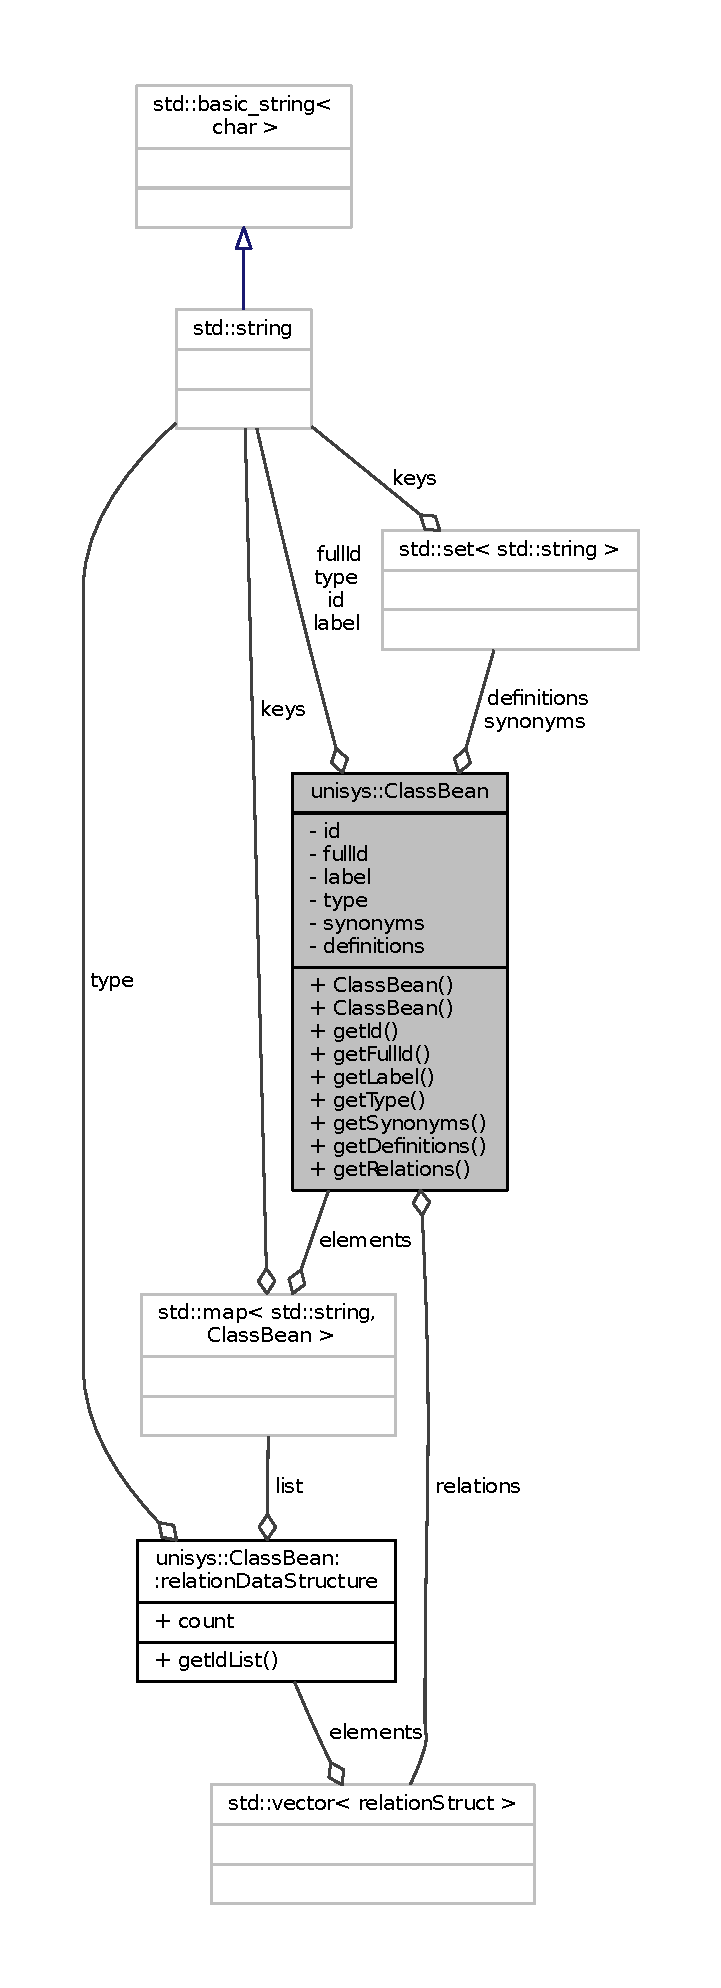
\includegraphics[height=550pt]{classunisys_1_1ClassBean__coll__graph}
\end{center}
\end{figure}
\subsection*{Classes}
\begin{DoxyCompactItemize}
\item 
struct \hyperlink{structunisys_1_1ClassBean_1_1relationDataStructure}{relation\-Data\-Structure}
\end{DoxyCompactItemize}
\subsection*{Public Types}
\begin{DoxyCompactItemize}
\item 
typedef struct \\*
\hyperlink{structunisys_1_1ClassBean_1_1relationDataStructure}{unisys\-::\-Class\-Bean\-::relation\-Data\-Structure} \hyperlink{classunisys_1_1ClassBean_aabeda0465f295816c6f784d7e3cbdb97}{relation\-Struct}
\begin{DoxyCompactList}\small\item\em For collecting the data in the relations node. \end{DoxyCompactList}\end{DoxyCompactItemize}
\subsection*{Public Member Functions}
\begin{DoxyCompactItemize}
\item 
\hyperlink{classunisys_1_1ClassBean_a48b70a5fa37a3ea8c0fedbfe63ffb963}{Class\-Bean} ()
\begin{DoxyCompactList}\small\item\em Default constructor. \end{DoxyCompactList}\item 
\hyperlink{classunisys_1_1ClassBean_a390c1b87bd723fd746f8151867961997}{Class\-Bean} (\hyperlink{structXMLNode}{X\-M\-L\-Node} xml)
\begin{DoxyCompactList}\small\item\em Overload constructor for parsing X\-M\-L response. \end{DoxyCompactList}\item 
std\-::string \hyperlink{classunisys_1_1ClassBean_ae1d0891bd0143a853914f218a14a08ff}{get\-Id} () const 
\begin{DoxyCompactList}\small\item\em Return id. \end{DoxyCompactList}\item 
std\-::string \hyperlink{classunisys_1_1ClassBean_a53387132779d106a7dee6c897066480d}{get\-Full\-Id} () const 
\begin{DoxyCompactList}\small\item\em Return full\-Id. \end{DoxyCompactList}\item 
std\-::string \hyperlink{classunisys_1_1ClassBean_a0a503067b948f19b098d3d71ec4a120b}{get\-Label} () const 
\begin{DoxyCompactList}\small\item\em Return label. \end{DoxyCompactList}\item 
std\-::string \hyperlink{classunisys_1_1ClassBean_a83fecb8b41c64cc29d172b380ce16816}{get\-Type} () const 
\begin{DoxyCompactList}\small\item\em Returntype. \end{DoxyCompactList}\item 
std\-::set$<$ std\-::string $>$ \hyperlink{classunisys_1_1ClassBean_a7e7e54c7c889d696cfc7fdb22ba4b861}{get\-Synonyms} () const 
\begin{DoxyCompactList}\small\item\em Return the list of synonym. \end{DoxyCompactList}\item 
std\-::set$<$ std\-::string $>$ \hyperlink{classunisys_1_1ClassBean_aaa76e4b0ade048567c4b8d52312ef1a9}{get\-Definitions} () const 
\begin{DoxyCompactList}\small\item\em Return the list of definition. \end{DoxyCompactList}\item 
std\-::vector$<$ \hyperlink{classunisys_1_1ClassBean_aabeda0465f295816c6f784d7e3cbdb97}{relation\-Struct} $>$ \hyperlink{classunisys_1_1ClassBean_a85e6aa6781b0379eb956fb1517496e82}{get\-Relations} () const 
\begin{DoxyCompactList}\small\item\em Return the list of relation data structure. \end{DoxyCompactList}\end{DoxyCompactItemize}
\subsection*{Private Attributes}
\begin{DoxyCompactItemize}
\item 
std\-::string \hyperlink{classunisys_1_1ClassBean_a0873b3a3895796ebf52f92860beea2a9}{id}
\begin{DoxyCompactList}\small\item\em I\-D. \end{DoxyCompactList}\item 
std\-::string \hyperlink{classunisys_1_1ClassBean_a99394c8ec3b4e477c7e44702e68310bb}{full\-Id}
\begin{DoxyCompactList}\small\item\em Full I\-D of the class in U\-R\-I format. \end{DoxyCompactList}\item 
std\-::string \hyperlink{classunisys_1_1ClassBean_ad68cdc52aa9e61e682f54cf5574d1b37}{label}
\item 
std\-::string \hyperlink{classunisys_1_1ClassBean_a3cd934e3687f96b0dc87a3fcafbec4ca}{type}
\item 
std\-::set$<$ std\-::string $>$ \hyperlink{classunisys_1_1ClassBean_a50623767ece8ef538c949558bfbc53af}{synonyms}
\item 
std\-::set$<$ std\-::string $>$ \hyperlink{classunisys_1_1ClassBean_af811d05369c1981390be001ad4b9b24d}{definitions}
\item 
std\-::vector$<$ \hyperlink{classunisys_1_1ClassBean_aabeda0465f295816c6f784d7e3cbdb97}{relation\-Struct} $>$ \hyperlink{classunisys_1_1ClassBean_a39022db9b3e14d792b3d73c7c85c253d}{relations}
\end{DoxyCompactItemize}


\subsection{Detailed Description}
This class is for taking care of the specific structure of response data call class\-Bean. 

This class is normally used for parsing the response of term command. 

\subsection{Member Typedef Documentation}
\hypertarget{classunisys_1_1ClassBean_aabeda0465f295816c6f784d7e3cbdb97}{\index{unisys\-::\-Class\-Bean@{unisys\-::\-Class\-Bean}!relation\-Struct@{relation\-Struct}}
\index{relation\-Struct@{relation\-Struct}!unisys::ClassBean@{unisys\-::\-Class\-Bean}}
\subsubsection[{relation\-Struct}]{\setlength{\rightskip}{0pt plus 5cm}{\bf unisys\-::\-Class\-Bean\-::relation\-Struct}}}\label{classunisys_1_1ClassBean_aabeda0465f295816c6f784d7e3cbdb97}


For collecting the data in the relations node. 



\subsection{Constructor \& Destructor Documentation}
\hypertarget{classunisys_1_1ClassBean_a48b70a5fa37a3ea8c0fedbfe63ffb963}{\index{unisys\-::\-Class\-Bean@{unisys\-::\-Class\-Bean}!Class\-Bean@{Class\-Bean}}
\index{Class\-Bean@{Class\-Bean}!unisys::ClassBean@{unisys\-::\-Class\-Bean}}
\subsubsection[{Class\-Bean}]{\setlength{\rightskip}{0pt plus 5cm}unisys\-::\-Class\-Bean\-::\-Class\-Bean (
\begin{DoxyParamCaption}
{}
\end{DoxyParamCaption}
)}}\label{classunisys_1_1ClassBean_a48b70a5fa37a3ea8c0fedbfe63ffb963}


Default constructor. 

\hypertarget{classunisys_1_1ClassBean_a390c1b87bd723fd746f8151867961997}{\index{unisys\-::\-Class\-Bean@{unisys\-::\-Class\-Bean}!Class\-Bean@{Class\-Bean}}
\index{Class\-Bean@{Class\-Bean}!unisys::ClassBean@{unisys\-::\-Class\-Bean}}
\subsubsection[{Class\-Bean}]{\setlength{\rightskip}{0pt plus 5cm}unisys\-::\-Class\-Bean\-::\-Class\-Bean (
\begin{DoxyParamCaption}
\item[{{\bf X\-M\-L\-Node}}]{xml}
\end{DoxyParamCaption}
)}}\label{classunisys_1_1ClassBean_a390c1b87bd723fd746f8151867961997}


Overload constructor for parsing X\-M\-L response. 



\subsection{Member Function Documentation}
\hypertarget{classunisys_1_1ClassBean_aaa76e4b0ade048567c4b8d52312ef1a9}{\index{unisys\-::\-Class\-Bean@{unisys\-::\-Class\-Bean}!get\-Definitions@{get\-Definitions}}
\index{get\-Definitions@{get\-Definitions}!unisys::ClassBean@{unisys\-::\-Class\-Bean}}
\subsubsection[{get\-Definitions}]{\setlength{\rightskip}{0pt plus 5cm}std\-::set$<$std\-::string$>$ unisys\-::\-Class\-Bean\-::get\-Definitions (
\begin{DoxyParamCaption}
{}
\end{DoxyParamCaption}
) const}}\label{classunisys_1_1ClassBean_aaa76e4b0ade048567c4b8d52312ef1a9}


Return the list of definition. 

\hypertarget{classunisys_1_1ClassBean_a53387132779d106a7dee6c897066480d}{\index{unisys\-::\-Class\-Bean@{unisys\-::\-Class\-Bean}!get\-Full\-Id@{get\-Full\-Id}}
\index{get\-Full\-Id@{get\-Full\-Id}!unisys::ClassBean@{unisys\-::\-Class\-Bean}}
\subsubsection[{get\-Full\-Id}]{\setlength{\rightskip}{0pt plus 5cm}std\-::string unisys\-::\-Class\-Bean\-::get\-Full\-Id (
\begin{DoxyParamCaption}
{}
\end{DoxyParamCaption}
) const}}\label{classunisys_1_1ClassBean_a53387132779d106a7dee6c897066480d}


Return full\-Id. 

\hypertarget{classunisys_1_1ClassBean_ae1d0891bd0143a853914f218a14a08ff}{\index{unisys\-::\-Class\-Bean@{unisys\-::\-Class\-Bean}!get\-Id@{get\-Id}}
\index{get\-Id@{get\-Id}!unisys::ClassBean@{unisys\-::\-Class\-Bean}}
\subsubsection[{get\-Id}]{\setlength{\rightskip}{0pt plus 5cm}std\-::string unisys\-::\-Class\-Bean\-::get\-Id (
\begin{DoxyParamCaption}
{}
\end{DoxyParamCaption}
) const}}\label{classunisys_1_1ClassBean_ae1d0891bd0143a853914f218a14a08ff}


Return id. 

\hypertarget{classunisys_1_1ClassBean_a0a503067b948f19b098d3d71ec4a120b}{\index{unisys\-::\-Class\-Bean@{unisys\-::\-Class\-Bean}!get\-Label@{get\-Label}}
\index{get\-Label@{get\-Label}!unisys::ClassBean@{unisys\-::\-Class\-Bean}}
\subsubsection[{get\-Label}]{\setlength{\rightskip}{0pt plus 5cm}std\-::string unisys\-::\-Class\-Bean\-::get\-Label (
\begin{DoxyParamCaption}
{}
\end{DoxyParamCaption}
) const}}\label{classunisys_1_1ClassBean_a0a503067b948f19b098d3d71ec4a120b}


Return label. 

\hypertarget{classunisys_1_1ClassBean_a85e6aa6781b0379eb956fb1517496e82}{\index{unisys\-::\-Class\-Bean@{unisys\-::\-Class\-Bean}!get\-Relations@{get\-Relations}}
\index{get\-Relations@{get\-Relations}!unisys::ClassBean@{unisys\-::\-Class\-Bean}}
\subsubsection[{get\-Relations}]{\setlength{\rightskip}{0pt plus 5cm}std\-::vector$<${\bf relation\-Struct}$>$ unisys\-::\-Class\-Bean\-::get\-Relations (
\begin{DoxyParamCaption}
{}
\end{DoxyParamCaption}
) const}}\label{classunisys_1_1ClassBean_a85e6aa6781b0379eb956fb1517496e82}


Return the list of relation data structure. 

\hypertarget{classunisys_1_1ClassBean_a7e7e54c7c889d696cfc7fdb22ba4b861}{\index{unisys\-::\-Class\-Bean@{unisys\-::\-Class\-Bean}!get\-Synonyms@{get\-Synonyms}}
\index{get\-Synonyms@{get\-Synonyms}!unisys::ClassBean@{unisys\-::\-Class\-Bean}}
\subsubsection[{get\-Synonyms}]{\setlength{\rightskip}{0pt plus 5cm}std\-::set$<$std\-::string$>$ unisys\-::\-Class\-Bean\-::get\-Synonyms (
\begin{DoxyParamCaption}
{}
\end{DoxyParamCaption}
) const}}\label{classunisys_1_1ClassBean_a7e7e54c7c889d696cfc7fdb22ba4b861}


Return the list of synonym. 

\hypertarget{classunisys_1_1ClassBean_a83fecb8b41c64cc29d172b380ce16816}{\index{unisys\-::\-Class\-Bean@{unisys\-::\-Class\-Bean}!get\-Type@{get\-Type}}
\index{get\-Type@{get\-Type}!unisys::ClassBean@{unisys\-::\-Class\-Bean}}
\subsubsection[{get\-Type}]{\setlength{\rightskip}{0pt plus 5cm}std\-::string unisys\-::\-Class\-Bean\-::get\-Type (
\begin{DoxyParamCaption}
{}
\end{DoxyParamCaption}
) const}}\label{classunisys_1_1ClassBean_a83fecb8b41c64cc29d172b380ce16816}


Returntype. 



\subsection{Member Data Documentation}
\hypertarget{classunisys_1_1ClassBean_af811d05369c1981390be001ad4b9b24d}{\index{unisys\-::\-Class\-Bean@{unisys\-::\-Class\-Bean}!definitions@{definitions}}
\index{definitions@{definitions}!unisys::ClassBean@{unisys\-::\-Class\-Bean}}
\subsubsection[{definitions}]{\setlength{\rightskip}{0pt plus 5cm}std\-::set$<$std\-::string$>$ unisys\-::\-Class\-Bean\-::definitions\hspace{0.3cm}{\ttfamily [private]}}}\label{classunisys_1_1ClassBean_af811d05369c1981390be001ad4b9b24d}
\hypertarget{classunisys_1_1ClassBean_a99394c8ec3b4e477c7e44702e68310bb}{\index{unisys\-::\-Class\-Bean@{unisys\-::\-Class\-Bean}!full\-Id@{full\-Id}}
\index{full\-Id@{full\-Id}!unisys::ClassBean@{unisys\-::\-Class\-Bean}}
\subsubsection[{full\-Id}]{\setlength{\rightskip}{0pt plus 5cm}std\-::string unisys\-::\-Class\-Bean\-::full\-Id\hspace{0.3cm}{\ttfamily [private]}}}\label{classunisys_1_1ClassBean_a99394c8ec3b4e477c7e44702e68310bb}


Full I\-D of the class in U\-R\-I format. 

\hypertarget{classunisys_1_1ClassBean_a0873b3a3895796ebf52f92860beea2a9}{\index{unisys\-::\-Class\-Bean@{unisys\-::\-Class\-Bean}!id@{id}}
\index{id@{id}!unisys::ClassBean@{unisys\-::\-Class\-Bean}}
\subsubsection[{id}]{\setlength{\rightskip}{0pt plus 5cm}std\-::string unisys\-::\-Class\-Bean\-::id\hspace{0.3cm}{\ttfamily [private]}}}\label{classunisys_1_1ClassBean_a0873b3a3895796ebf52f92860beea2a9}


I\-D. 

\hypertarget{classunisys_1_1ClassBean_ad68cdc52aa9e61e682f54cf5574d1b37}{\index{unisys\-::\-Class\-Bean@{unisys\-::\-Class\-Bean}!label@{label}}
\index{label@{label}!unisys::ClassBean@{unisys\-::\-Class\-Bean}}
\subsubsection[{label}]{\setlength{\rightskip}{0pt plus 5cm}std\-::string unisys\-::\-Class\-Bean\-::label\hspace{0.3cm}{\ttfamily [private]}}}\label{classunisys_1_1ClassBean_ad68cdc52aa9e61e682f54cf5574d1b37}
\hypertarget{classunisys_1_1ClassBean_a39022db9b3e14d792b3d73c7c85c253d}{\index{unisys\-::\-Class\-Bean@{unisys\-::\-Class\-Bean}!relations@{relations}}
\index{relations@{relations}!unisys::ClassBean@{unisys\-::\-Class\-Bean}}
\subsubsection[{relations}]{\setlength{\rightskip}{0pt plus 5cm}std\-::vector$<${\bf relation\-Struct}$>$ unisys\-::\-Class\-Bean\-::relations\hspace{0.3cm}{\ttfamily [private]}}}\label{classunisys_1_1ClassBean_a39022db9b3e14d792b3d73c7c85c253d}
\hypertarget{classunisys_1_1ClassBean_a50623767ece8ef538c949558bfbc53af}{\index{unisys\-::\-Class\-Bean@{unisys\-::\-Class\-Bean}!synonyms@{synonyms}}
\index{synonyms@{synonyms}!unisys::ClassBean@{unisys\-::\-Class\-Bean}}
\subsubsection[{synonyms}]{\setlength{\rightskip}{0pt plus 5cm}std\-::set$<$std\-::string$>$ unisys\-::\-Class\-Bean\-::synonyms\hspace{0.3cm}{\ttfamily [private]}}}\label{classunisys_1_1ClassBean_a50623767ece8ef538c949558bfbc53af}
\hypertarget{classunisys_1_1ClassBean_a3cd934e3687f96b0dc87a3fcafbec4ca}{\index{unisys\-::\-Class\-Bean@{unisys\-::\-Class\-Bean}!type@{type}}
\index{type@{type}!unisys::ClassBean@{unisys\-::\-Class\-Bean}}
\subsubsection[{type}]{\setlength{\rightskip}{0pt plus 5cm}std\-::string unisys\-::\-Class\-Bean\-::type\hspace{0.3cm}{\ttfamily [private]}}}\label{classunisys_1_1ClassBean_a3cd934e3687f96b0dc87a3fcafbec4ca}


The documentation for this class was generated from the following file\-:\begin{DoxyCompactItemize}
\item 
\hyperlink{restBioPortal_8h}{rest\-Bio\-Portal.\-h}\end{DoxyCompactItemize}

\hypertarget{classunisys_1_1Complex}{\section{unisys\-:\-:Complex Class Reference}
\label{classunisys_1_1Complex}\index{unisys\-::\-Complex@{unisys\-::\-Complex}}
}


This class is for miriam cross reference annotation.  




{\ttfamily \#include $<$Obj\-Class.\-h$>$}



Inheritance diagram for unisys\-:\-:Complex\-:
\nopagebreak
\begin{figure}[H]
\begin{center}
\leavevmode
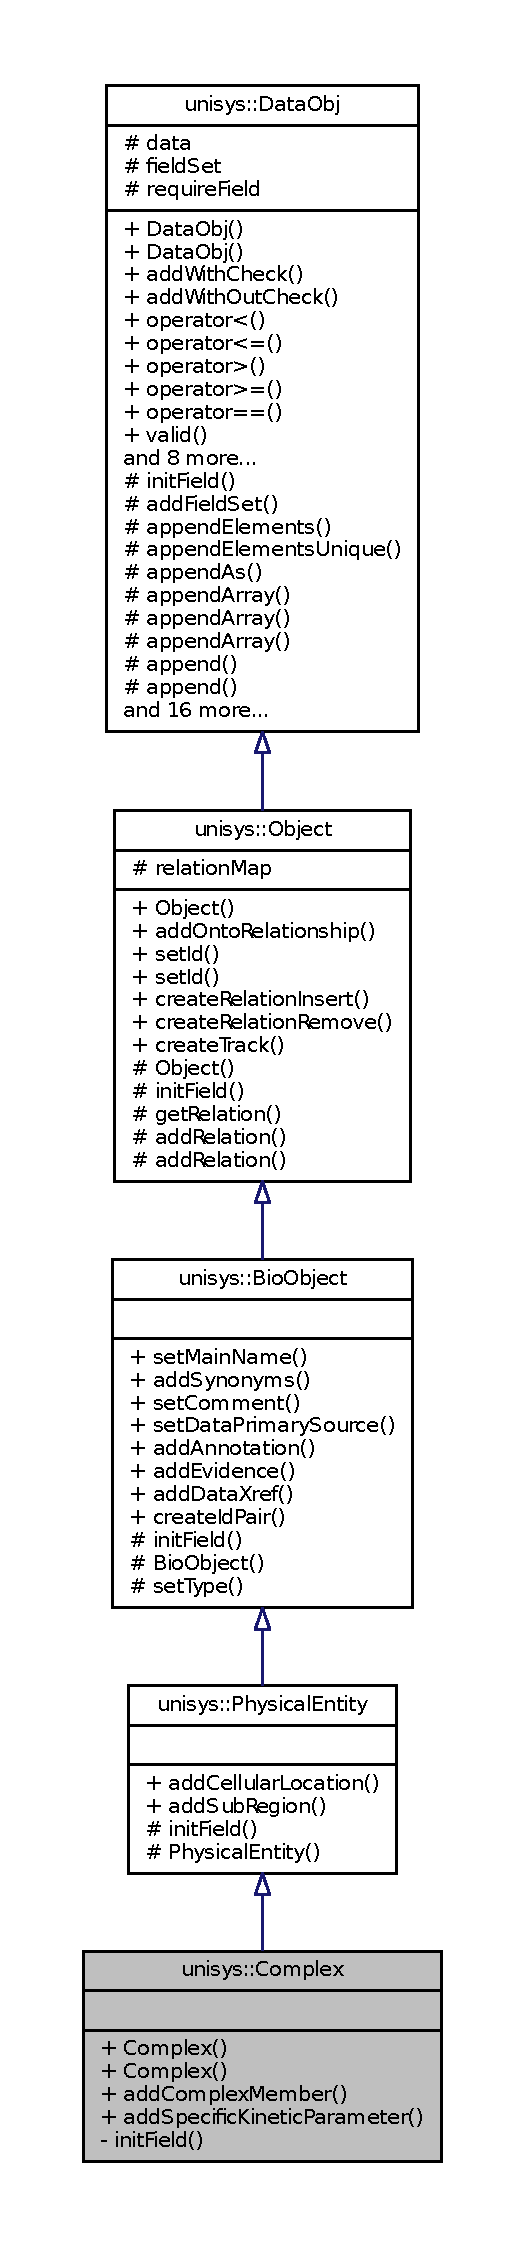
\includegraphics[height=550pt]{classunisys_1_1Complex__inherit__graph}
\end{center}
\end{figure}


Collaboration diagram for unisys\-:\-:Complex\-:
\nopagebreak
\begin{figure}[H]
\begin{center}
\leavevmode
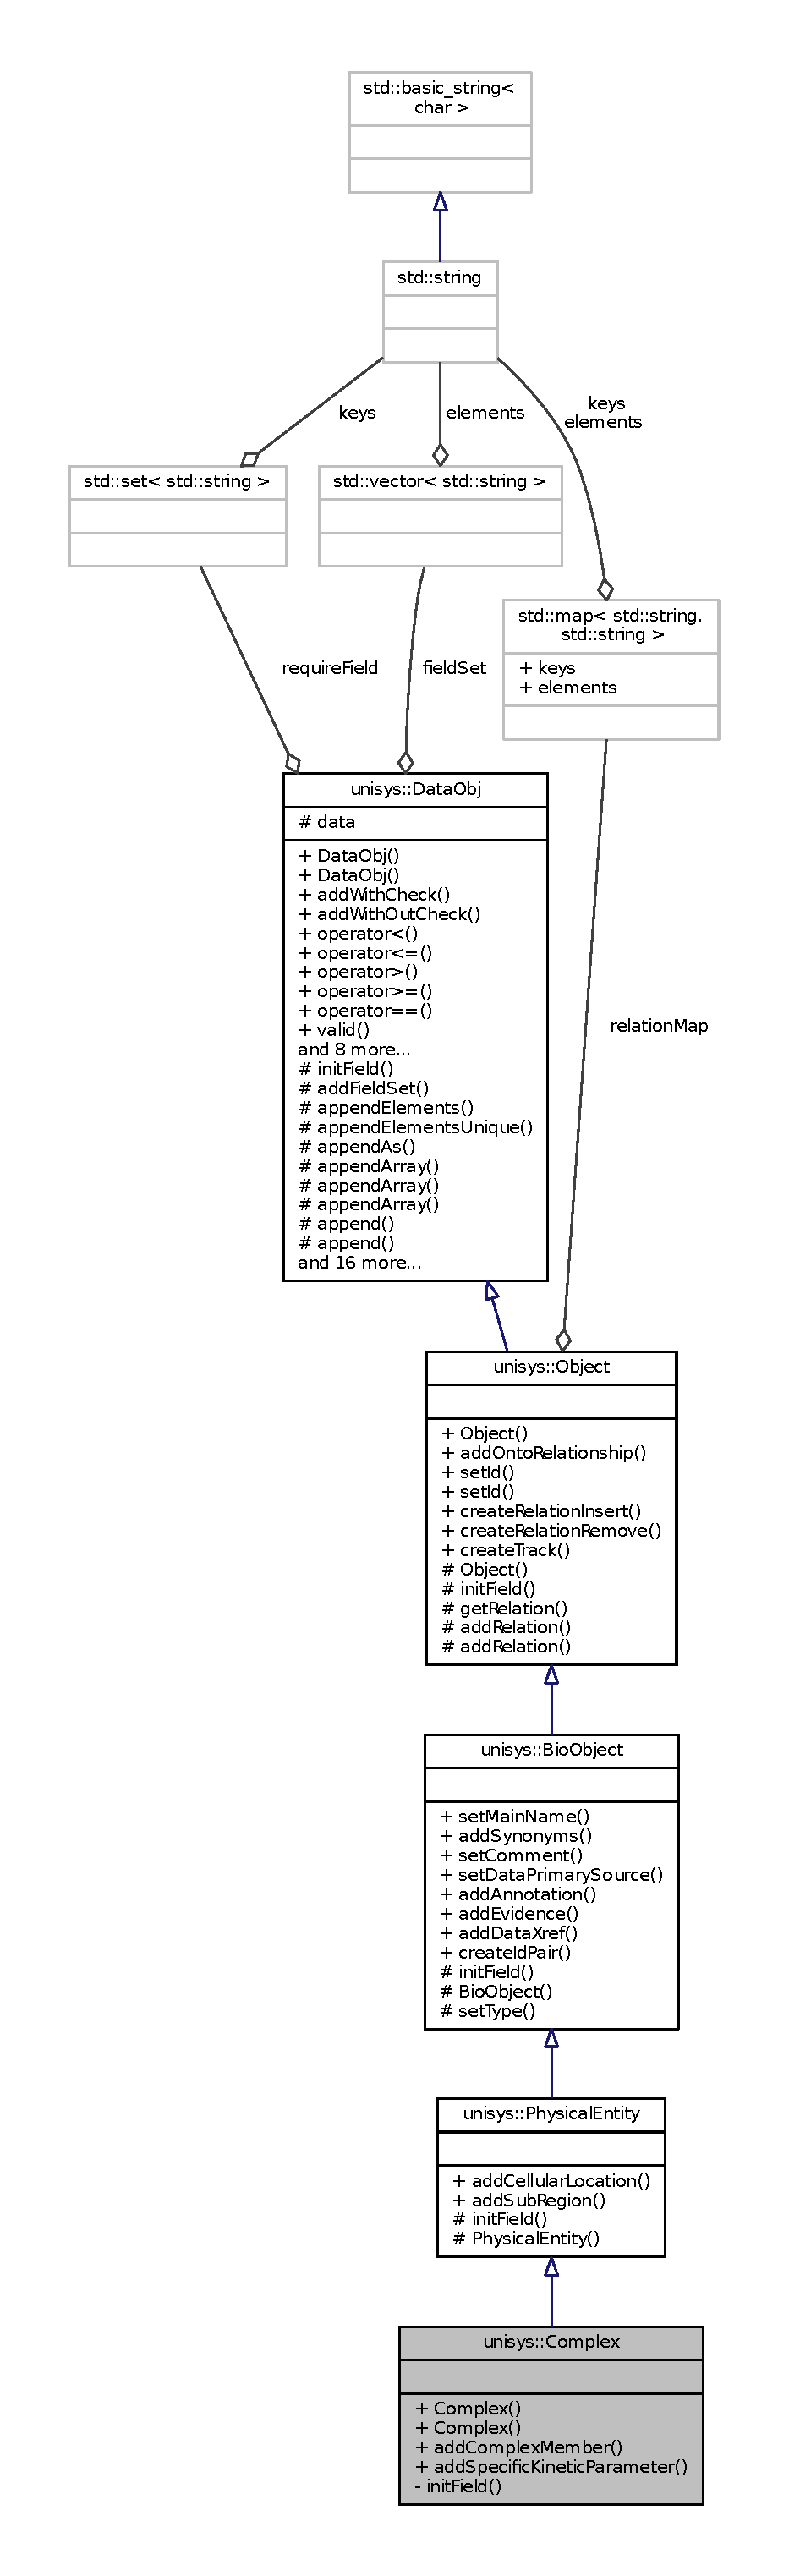
\includegraphics[height=550pt]{classunisys_1_1Complex__coll__graph}
\end{center}
\end{figure}
\subsection*{Public Member Functions}
\begin{DoxyCompactItemize}
\item 
\hyperlink{classunisys_1_1Complex_af1f053767f82558fca1aacbe506c80b3}{Complex} ()
\begin{DoxyCompactList}\small\item\em Default constructor. \end{DoxyCompactList}\item 
\hyperlink{classunisys_1_1Complex_adf5a0991130d29373856723ca7c90e69}{Complex} (mongo\-::\-B\-S\-O\-N\-Obj const \&bson\-Obj)
\begin{DoxyCompactList}\small\item\em Overloaded constructor is used when retriving data in boson object from database and tranform to C++ object. \end{DoxyCompactList}\item 
void \hyperlink{classunisys_1_1Complex_a31f85126c8248ca57b0a64a54fa8f10f}{add\-Complex\-Member} (\hyperlink{classunisys_1_1PEIdRef}{P\-E\-Id\-Ref} \&pe\-Id\-Ref)
\item 
void \hyperlink{classunisys_1_1Complex_af60845ea26c2e255e3d707a45ce67717}{add\-Specific\-Kinetic\-Parameter} (\hyperlink{classunisys_1_1KineticParameter}{Kinetic\-Parameter} \&kinetic\-Parameter)
\end{DoxyCompactItemize}
\subsection*{Private Member Functions}
\begin{DoxyCompactItemize}
\item 
void \hyperlink{classunisys_1_1Complex_a63e019fcca3e2d919937694678d9ee1f}{init\-Field} ()
\end{DoxyCompactItemize}
\subsection*{Additional Inherited Members}


\subsection{Detailed Description}
This class is for miriam cross reference annotation. 

\begin{DoxyVerb}        BSON structure:
        {   
            _id: <string>, #madatory
            ontologyRelationship: {<RelationshipBOSON>, <RelationshipBOSON>, ...},
            name: {<string>,<string>, ...}
            comment: <string>,
            dataPrimarySource: <XrefBOSON>,
            functionAnnotation: {<AnnotationBOSON>, <AnnotationBOSON>, ...},
            evidence: {<EvidenceBOSON>, <EvidenceBOSON>, ...},
            dataxref: {<XrefBOSON>, <XrefBOSON>, ...},
            interaction: {<DbRef>, <DbRef>, ...},
            complex: {<DbRef>, <DbRef>, ...},
            subRegion: {<SubRegionBOSON>, <SubRegionBOSON>, ...},
            complexMember: {<DbRef>, <DbRef>, ...},
            specificKineticParameter: {<KineticParameterBOSON>, <KineticParameterBOSON>, ...}
        }\end{DoxyVerb}
 

\subsection{Constructor \& Destructor Documentation}
\hypertarget{classunisys_1_1Complex_af1f053767f82558fca1aacbe506c80b3}{\index{unisys\-::\-Complex@{unisys\-::\-Complex}!Complex@{Complex}}
\index{Complex@{Complex}!unisys::Complex@{unisys\-::\-Complex}}
\subsubsection[{Complex}]{\setlength{\rightskip}{0pt plus 5cm}unisys\-::\-Complex\-::\-Complex (
\begin{DoxyParamCaption}
{}
\end{DoxyParamCaption}
)}}\label{classunisys_1_1Complex_af1f053767f82558fca1aacbe506c80b3}


Default constructor. 

\hypertarget{classunisys_1_1Complex_adf5a0991130d29373856723ca7c90e69}{\index{unisys\-::\-Complex@{unisys\-::\-Complex}!Complex@{Complex}}
\index{Complex@{Complex}!unisys::Complex@{unisys\-::\-Complex}}
\subsubsection[{Complex}]{\setlength{\rightskip}{0pt plus 5cm}unisys\-::\-Complex\-::\-Complex (
\begin{DoxyParamCaption}
\item[{mongo\-::\-B\-S\-O\-N\-Obj const \&}]{bson\-Obj}
\end{DoxyParamCaption}
)}}\label{classunisys_1_1Complex_adf5a0991130d29373856723ca7c90e69}


Overloaded constructor is used when retriving data in boson object from database and tranform to C++ object. 



\subsection{Member Function Documentation}
\hypertarget{classunisys_1_1Complex_a31f85126c8248ca57b0a64a54fa8f10f}{\index{unisys\-::\-Complex@{unisys\-::\-Complex}!add\-Complex\-Member@{add\-Complex\-Member}}
\index{add\-Complex\-Member@{add\-Complex\-Member}!unisys::Complex@{unisys\-::\-Complex}}
\subsubsection[{add\-Complex\-Member}]{\setlength{\rightskip}{0pt plus 5cm}void unisys\-::\-Complex\-::add\-Complex\-Member (
\begin{DoxyParamCaption}
\item[{{\bf P\-E\-Id\-Ref} \&}]{pe\-Id\-Ref}
\end{DoxyParamCaption}
)}}\label{classunisys_1_1Complex_a31f85126c8248ca57b0a64a54fa8f10f}
\hypertarget{classunisys_1_1Complex_af60845ea26c2e255e3d707a45ce67717}{\index{unisys\-::\-Complex@{unisys\-::\-Complex}!add\-Specific\-Kinetic\-Parameter@{add\-Specific\-Kinetic\-Parameter}}
\index{add\-Specific\-Kinetic\-Parameter@{add\-Specific\-Kinetic\-Parameter}!unisys::Complex@{unisys\-::\-Complex}}
\subsubsection[{add\-Specific\-Kinetic\-Parameter}]{\setlength{\rightskip}{0pt plus 5cm}void unisys\-::\-Complex\-::add\-Specific\-Kinetic\-Parameter (
\begin{DoxyParamCaption}
\item[{{\bf Kinetic\-Parameter} \&}]{kinetic\-Parameter}
\end{DoxyParamCaption}
)}}\label{classunisys_1_1Complex_af60845ea26c2e255e3d707a45ce67717}
\hypertarget{classunisys_1_1Complex_a63e019fcca3e2d919937694678d9ee1f}{\index{unisys\-::\-Complex@{unisys\-::\-Complex}!init\-Field@{init\-Field}}
\index{init\-Field@{init\-Field}!unisys::Complex@{unisys\-::\-Complex}}
\subsubsection[{init\-Field}]{\setlength{\rightskip}{0pt plus 5cm}void unisys\-::\-Complex\-::init\-Field (
\begin{DoxyParamCaption}
{}
\end{DoxyParamCaption}
)\hspace{0.3cm}{\ttfamily [private]}, {\ttfamily [virtual]}}}\label{classunisys_1_1Complex_a63e019fcca3e2d919937694678d9ee1f}


Reimplemented from \hyperlink{classunisys_1_1PhysicalEntity_ad445727cb6b1c12e954819d8207104e8}{unisys\-::\-Physical\-Entity}.



The documentation for this class was generated from the following file\-:\begin{DoxyCompactItemize}
\item 
\hyperlink{ObjClass_8h}{Obj\-Class.\-h}\end{DoxyCompactItemize}

\hypertarget{classunisys_1_1ConnectionError}{\section{unisys\-:\-:Connection\-Error Class Reference}
\label{classunisys_1_1ConnectionError}\index{unisys\-::\-Connection\-Error@{unisys\-::\-Connection\-Error}}
}


{\ttfamily \#include $<$exception.\-h$>$}



Inheritance diagram for unisys\-:\-:Connection\-Error\-:
\nopagebreak
\begin{figure}[H]
\begin{center}
\leavevmode
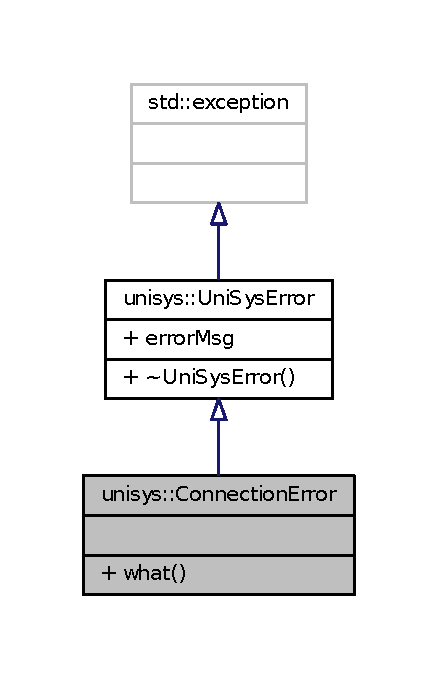
\includegraphics[width=210pt]{classunisys_1_1ConnectionError__inherit__graph}
\end{center}
\end{figure}


Collaboration diagram for unisys\-:\-:Connection\-Error\-:
\nopagebreak
\begin{figure}[H]
\begin{center}
\leavevmode
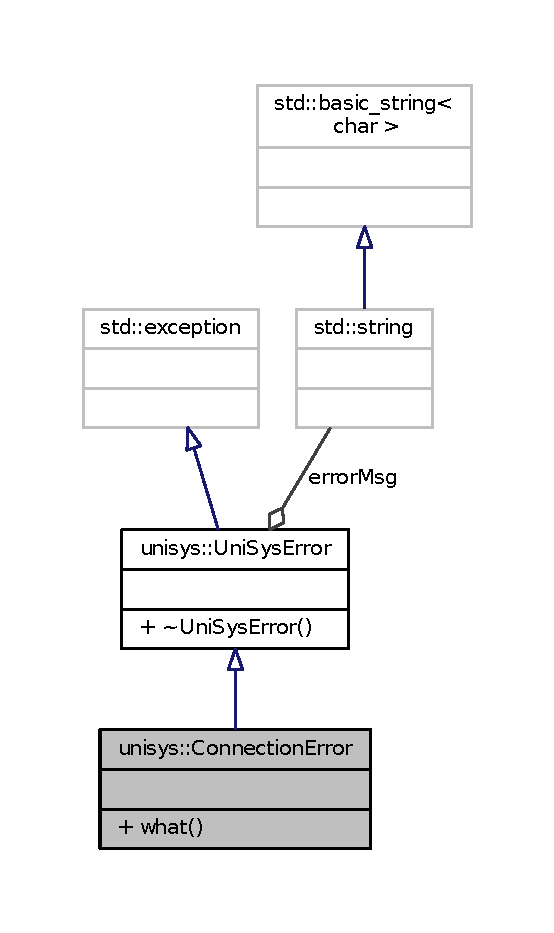
\includegraphics[width=266pt]{classunisys_1_1ConnectionError__coll__graph}
\end{center}
\end{figure}
\subsection*{Public Member Functions}
\begin{DoxyCompactItemize}
\item 
virtual const char $\ast$ \hyperlink{classunisys_1_1ConnectionError_a94eecd4cfb582f7440ba5f7086e3cb9e}{what} () const   throw ()
\end{DoxyCompactItemize}
\subsection*{Additional Inherited Members}


\subsection{Member Function Documentation}
\hypertarget{classunisys_1_1ConnectionError_a94eecd4cfb582f7440ba5f7086e3cb9e}{\index{unisys\-::\-Connection\-Error@{unisys\-::\-Connection\-Error}!what@{what}}
\index{what@{what}!unisys::ConnectionError@{unisys\-::\-Connection\-Error}}
\subsubsection[{what}]{\setlength{\rightskip}{0pt plus 5cm}virtual const char$\ast$ unisys\-::\-Connection\-Error\-::what (
\begin{DoxyParamCaption}
{}
\end{DoxyParamCaption}
) const  throw ()\hspace{0.3cm}{\ttfamily [inline]}, {\ttfamily [virtual]}}}\label{classunisys_1_1ConnectionError_a94eecd4cfb582f7440ba5f7086e3cb9e}


The documentation for this class was generated from the following file\-:\begin{DoxyCompactItemize}
\item 
\hyperlink{exception_8h}{exception.\-h}\end{DoxyCompactItemize}

\hypertarget{classunisys_1_1Control}{\section{unisys\-:\-:Control Class Reference}
\label{classunisys_1_1Control}\index{unisys\-::\-Control@{unisys\-::\-Control}}
}


This class is for miriam cross reference annotation.  




{\ttfamily \#include $<$Obj\-Class.\-h$>$}



Inheritance diagram for unisys\-:\-:Control\-:
\nopagebreak
\begin{figure}[H]
\begin{center}
\leavevmode
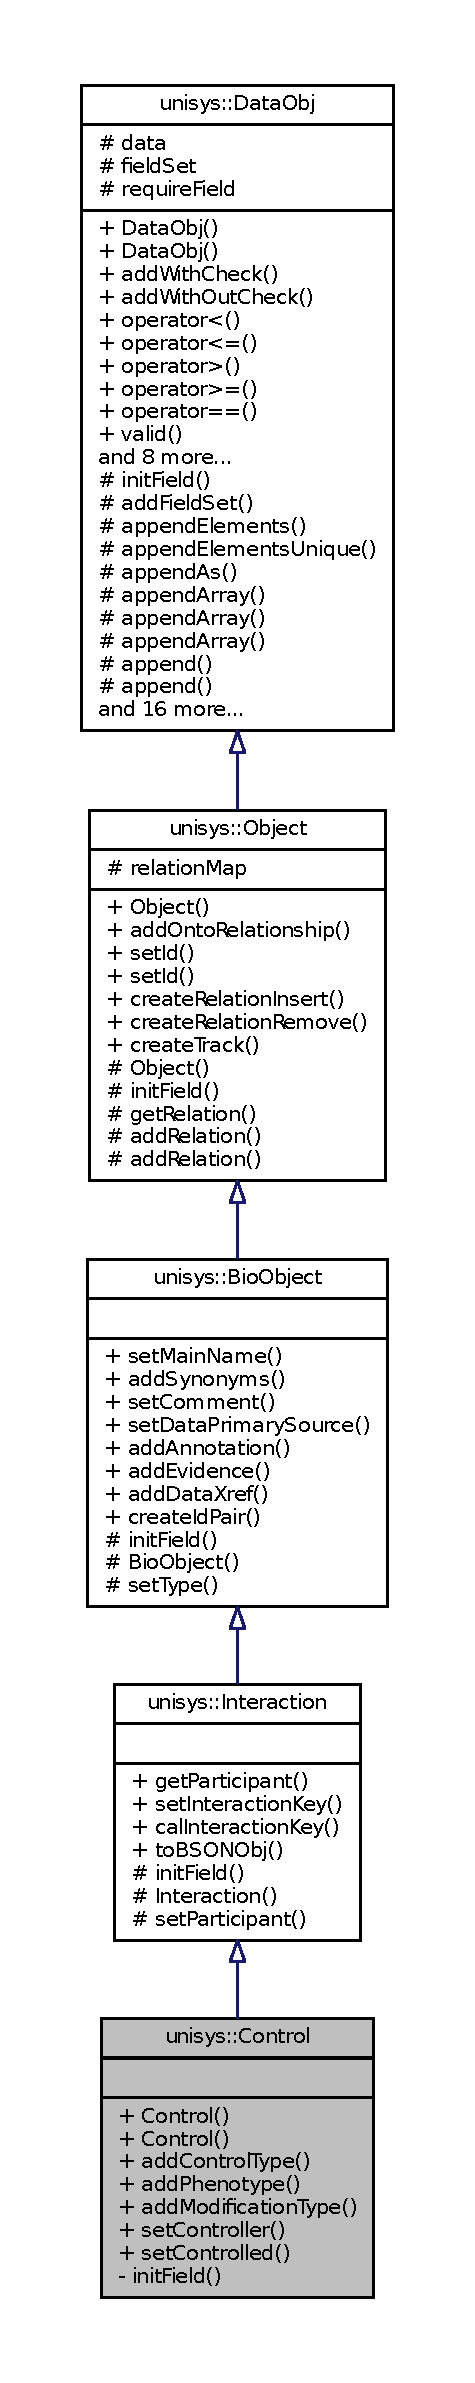
\includegraphics[height=550pt]{classunisys_1_1Control__inherit__graph}
\end{center}
\end{figure}


Collaboration diagram for unisys\-:\-:Control\-:
\nopagebreak
\begin{figure}[H]
\begin{center}
\leavevmode
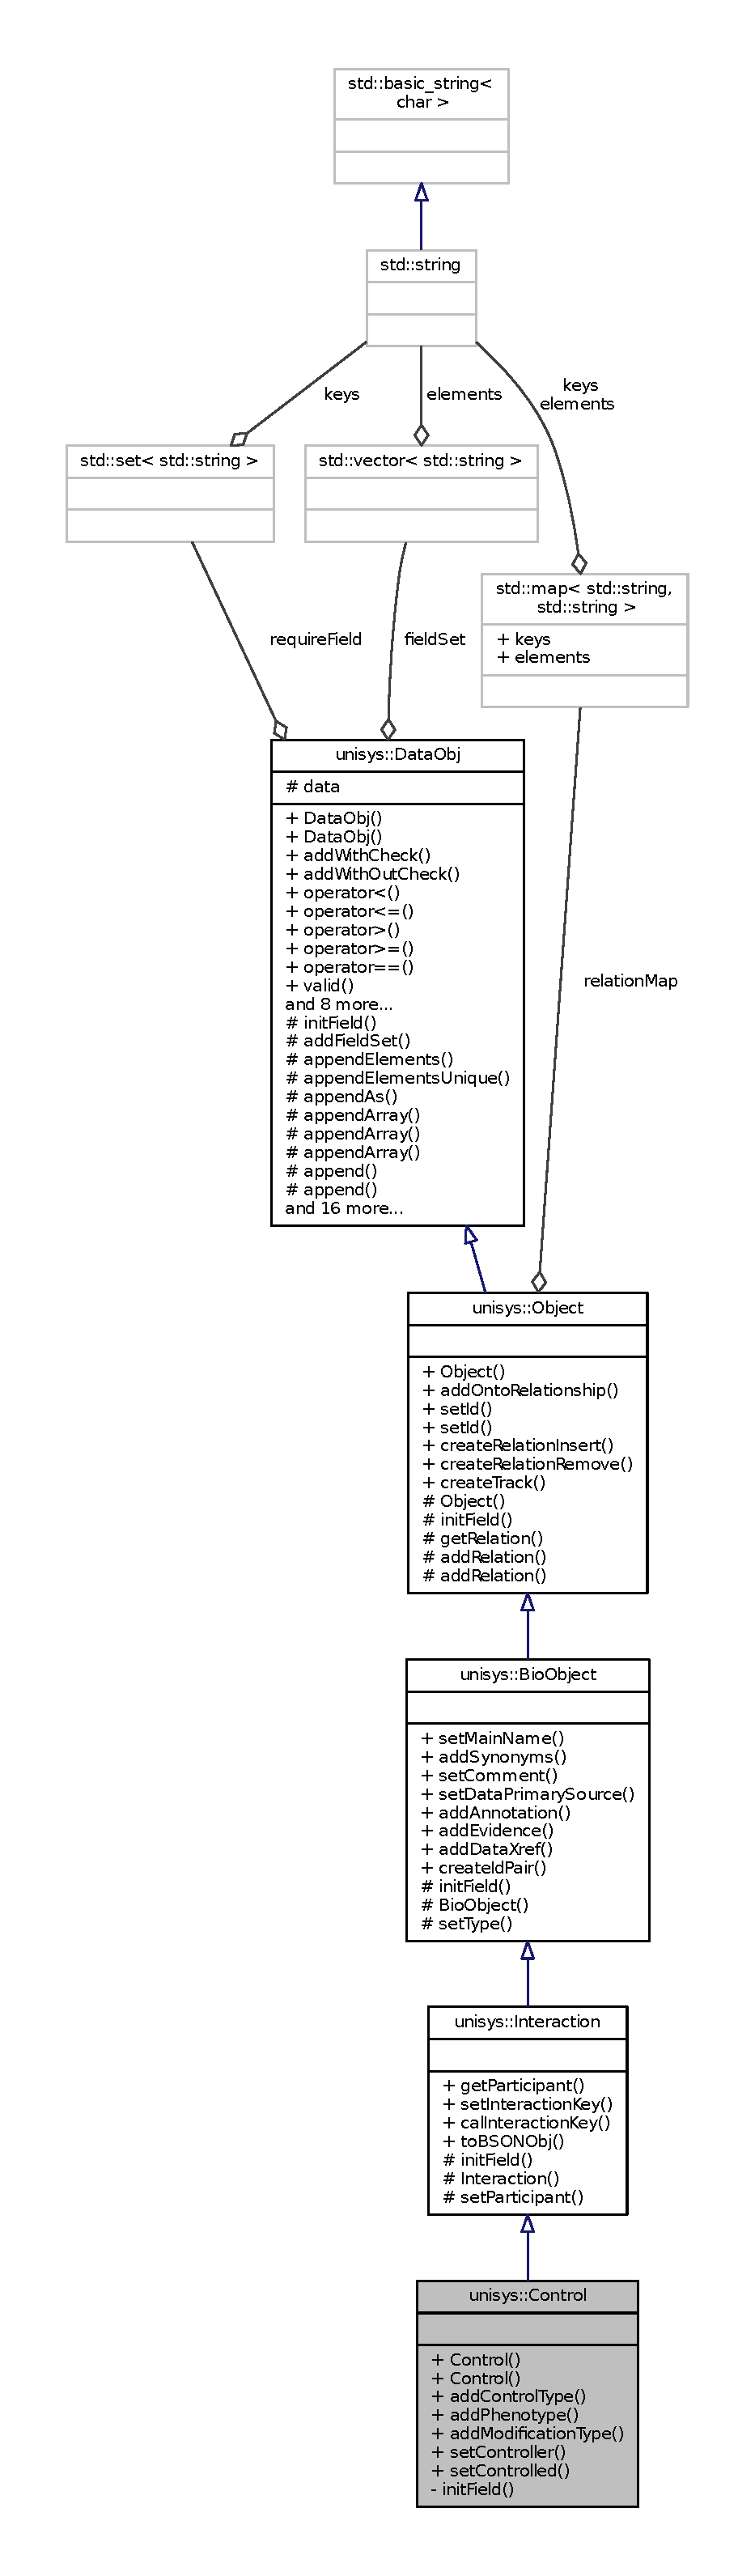
\includegraphics[height=550pt]{classunisys_1_1Control__coll__graph}
\end{center}
\end{figure}
\subsection*{Public Member Functions}
\begin{DoxyCompactItemize}
\item 
\hyperlink{classunisys_1_1Control_a45a42fd37436cba1202d12315f5258be}{Control} ()
\begin{DoxyCompactList}\small\item\em Default constructor. \end{DoxyCompactList}\item 
\hyperlink{classunisys_1_1Control_a762428d4e00ddf84baf7f1a020ab5b6d}{Control} (mongo\-::\-B\-S\-O\-N\-Obj const \&bson\-Obj)
\begin{DoxyCompactList}\small\item\em Overloaded constructor is used when retriving data in boson object from database and tranform to C++ object. \end{DoxyCompactList}\item 
void \hyperlink{classunisys_1_1Control_acfb48716bae9c0e0b8de04c31449db3b}{add\-Control\-Type} (\hyperlink{classunisys_1_1OntoIdRef}{Onto\-Id\-Ref} \&onto\-Id\-Ref)
\item 
void \hyperlink{classunisys_1_1Control_a5e008209a9c599b1aec5da00587f6297}{add\-Phenotype} (\hyperlink{classunisys_1_1OntoIdRef}{Onto\-Id\-Ref} \&onto\-Id\-Ref)
\item 
void \hyperlink{classunisys_1_1Control_aad4208e0899fa38f1160c16593c66f03}{add\-Modification\-Type} (\hyperlink{classunisys_1_1OntoIdRef}{Onto\-Id\-Ref} \&onto\-Id\-Ref)
\item 
void \hyperlink{classunisys_1_1Control_afcf95fc81aebf501b35f1cc11c7edc70}{set\-Controller} (\hyperlink{classunisys_1_1PEIdRef}{P\-E\-Id\-Ref} \&pe\-Id\-Ref)
\item 
void \hyperlink{classunisys_1_1Control_abdf99d44981306596d7120c46ea2a84f}{set\-Controlled} (\hyperlink{classunisys_1_1PEIdRef}{P\-E\-Id\-Ref} \&pe\-Id\-Ref)
\end{DoxyCompactItemize}
\subsection*{Private Member Functions}
\begin{DoxyCompactItemize}
\item 
void \hyperlink{classunisys_1_1Control_ab5bd5022b73b81e3fd18af06027213b1}{init\-Field} ()
\end{DoxyCompactItemize}
\subsection*{Additional Inherited Members}


\subsection{Detailed Description}
This class is for miriam cross reference annotation. 

\begin{DoxyVerb}        BSON structure:
        {   
            _id: <string>, #madatory
            type: <string>,
            ontologyRelationship: {<RelationshipBOSON>, <RelationshipBOSON>, ...},
            name: {<string>,<string>, ...}
            comment: <string>,
            dataPrimarySource: <XrefBOSON>,
            functionAnnotation: {<AnnotationBOSON>, <AnnotationBOSON>, ...},
            evidence: {<EvidenceBOSON>, <EvidenceBOSON>, ...},
            dataxref: {<XrefBOSON>, <XrefBOSON>, ...},
            participant: {<StoichiometryBOSON>, <StoichiometryBOSON>, ...},
            interactionKey: <string>,
            controlType: {<DbRef>, <DbRef>, ...},
            phenotype: {<DbRef>, <DbRef>, ...},
            modificationType: {<DbRef>, <DbRef>, ...}
        }\end{DoxyVerb}
 

\subsection{Constructor \& Destructor Documentation}
\hypertarget{classunisys_1_1Control_a45a42fd37436cba1202d12315f5258be}{\index{unisys\-::\-Control@{unisys\-::\-Control}!Control@{Control}}
\index{Control@{Control}!unisys::Control@{unisys\-::\-Control}}
\subsubsection[{Control}]{\setlength{\rightskip}{0pt plus 5cm}unisys\-::\-Control\-::\-Control (
\begin{DoxyParamCaption}
{}
\end{DoxyParamCaption}
)}}\label{classunisys_1_1Control_a45a42fd37436cba1202d12315f5258be}


Default constructor. 

\hypertarget{classunisys_1_1Control_a762428d4e00ddf84baf7f1a020ab5b6d}{\index{unisys\-::\-Control@{unisys\-::\-Control}!Control@{Control}}
\index{Control@{Control}!unisys::Control@{unisys\-::\-Control}}
\subsubsection[{Control}]{\setlength{\rightskip}{0pt plus 5cm}unisys\-::\-Control\-::\-Control (
\begin{DoxyParamCaption}
\item[{mongo\-::\-B\-S\-O\-N\-Obj const \&}]{bson\-Obj}
\end{DoxyParamCaption}
)}}\label{classunisys_1_1Control_a762428d4e00ddf84baf7f1a020ab5b6d}


Overloaded constructor is used when retriving data in boson object from database and tranform to C++ object. 



\subsection{Member Function Documentation}
\hypertarget{classunisys_1_1Control_acfb48716bae9c0e0b8de04c31449db3b}{\index{unisys\-::\-Control@{unisys\-::\-Control}!add\-Control\-Type@{add\-Control\-Type}}
\index{add\-Control\-Type@{add\-Control\-Type}!unisys::Control@{unisys\-::\-Control}}
\subsubsection[{add\-Control\-Type}]{\setlength{\rightskip}{0pt plus 5cm}void unisys\-::\-Control\-::add\-Control\-Type (
\begin{DoxyParamCaption}
\item[{{\bf Onto\-Id\-Ref} \&}]{onto\-Id\-Ref}
\end{DoxyParamCaption}
)}}\label{classunisys_1_1Control_acfb48716bae9c0e0b8de04c31449db3b}
\hypertarget{classunisys_1_1Control_aad4208e0899fa38f1160c16593c66f03}{\index{unisys\-::\-Control@{unisys\-::\-Control}!add\-Modification\-Type@{add\-Modification\-Type}}
\index{add\-Modification\-Type@{add\-Modification\-Type}!unisys::Control@{unisys\-::\-Control}}
\subsubsection[{add\-Modification\-Type}]{\setlength{\rightskip}{0pt plus 5cm}void unisys\-::\-Control\-::add\-Modification\-Type (
\begin{DoxyParamCaption}
\item[{{\bf Onto\-Id\-Ref} \&}]{onto\-Id\-Ref}
\end{DoxyParamCaption}
)}}\label{classunisys_1_1Control_aad4208e0899fa38f1160c16593c66f03}
\hypertarget{classunisys_1_1Control_a5e008209a9c599b1aec5da00587f6297}{\index{unisys\-::\-Control@{unisys\-::\-Control}!add\-Phenotype@{add\-Phenotype}}
\index{add\-Phenotype@{add\-Phenotype}!unisys::Control@{unisys\-::\-Control}}
\subsubsection[{add\-Phenotype}]{\setlength{\rightskip}{0pt plus 5cm}void unisys\-::\-Control\-::add\-Phenotype (
\begin{DoxyParamCaption}
\item[{{\bf Onto\-Id\-Ref} \&}]{onto\-Id\-Ref}
\end{DoxyParamCaption}
)}}\label{classunisys_1_1Control_a5e008209a9c599b1aec5da00587f6297}
\hypertarget{classunisys_1_1Control_ab5bd5022b73b81e3fd18af06027213b1}{\index{unisys\-::\-Control@{unisys\-::\-Control}!init\-Field@{init\-Field}}
\index{init\-Field@{init\-Field}!unisys::Control@{unisys\-::\-Control}}
\subsubsection[{init\-Field}]{\setlength{\rightskip}{0pt plus 5cm}void unisys\-::\-Control\-::init\-Field (
\begin{DoxyParamCaption}
{}
\end{DoxyParamCaption}
)\hspace{0.3cm}{\ttfamily [private]}, {\ttfamily [virtual]}}}\label{classunisys_1_1Control_ab5bd5022b73b81e3fd18af06027213b1}


Reimplemented from \hyperlink{classunisys_1_1Interaction_a84c6c3e09f83ec8dd8dec7485f97e02b}{unisys\-::\-Interaction}.

\hypertarget{classunisys_1_1Control_abdf99d44981306596d7120c46ea2a84f}{\index{unisys\-::\-Control@{unisys\-::\-Control}!set\-Controlled@{set\-Controlled}}
\index{set\-Controlled@{set\-Controlled}!unisys::Control@{unisys\-::\-Control}}
\subsubsection[{set\-Controlled}]{\setlength{\rightskip}{0pt plus 5cm}void unisys\-::\-Control\-::set\-Controlled (
\begin{DoxyParamCaption}
\item[{{\bf P\-E\-Id\-Ref} \&}]{pe\-Id\-Ref}
\end{DoxyParamCaption}
)}}\label{classunisys_1_1Control_abdf99d44981306596d7120c46ea2a84f}
\hypertarget{classunisys_1_1Control_afcf95fc81aebf501b35f1cc11c7edc70}{\index{unisys\-::\-Control@{unisys\-::\-Control}!set\-Controller@{set\-Controller}}
\index{set\-Controller@{set\-Controller}!unisys::Control@{unisys\-::\-Control}}
\subsubsection[{set\-Controller}]{\setlength{\rightskip}{0pt plus 5cm}void unisys\-::\-Control\-::set\-Controller (
\begin{DoxyParamCaption}
\item[{{\bf P\-E\-Id\-Ref} \&}]{pe\-Id\-Ref}
\end{DoxyParamCaption}
)}}\label{classunisys_1_1Control_afcf95fc81aebf501b35f1cc11c7edc70}


The documentation for this class was generated from the following file\-:\begin{DoxyCompactItemize}
\item 
\hyperlink{ObjClass_8h}{Obj\-Class.\-h}\end{DoxyCompactItemize}

\hypertarget{classunisys_1_1Conversion}{\section{unisys\-:\-:Conversion Class Reference}
\label{classunisys_1_1Conversion}\index{unisys\-::\-Conversion@{unisys\-::\-Conversion}}
}


This class is for miriam cross reference annotation.  




{\ttfamily \#include $<$Obj\-Class.\-h$>$}



Inheritance diagram for unisys\-:\-:Conversion\-:
\nopagebreak
\begin{figure}[H]
\begin{center}
\leavevmode
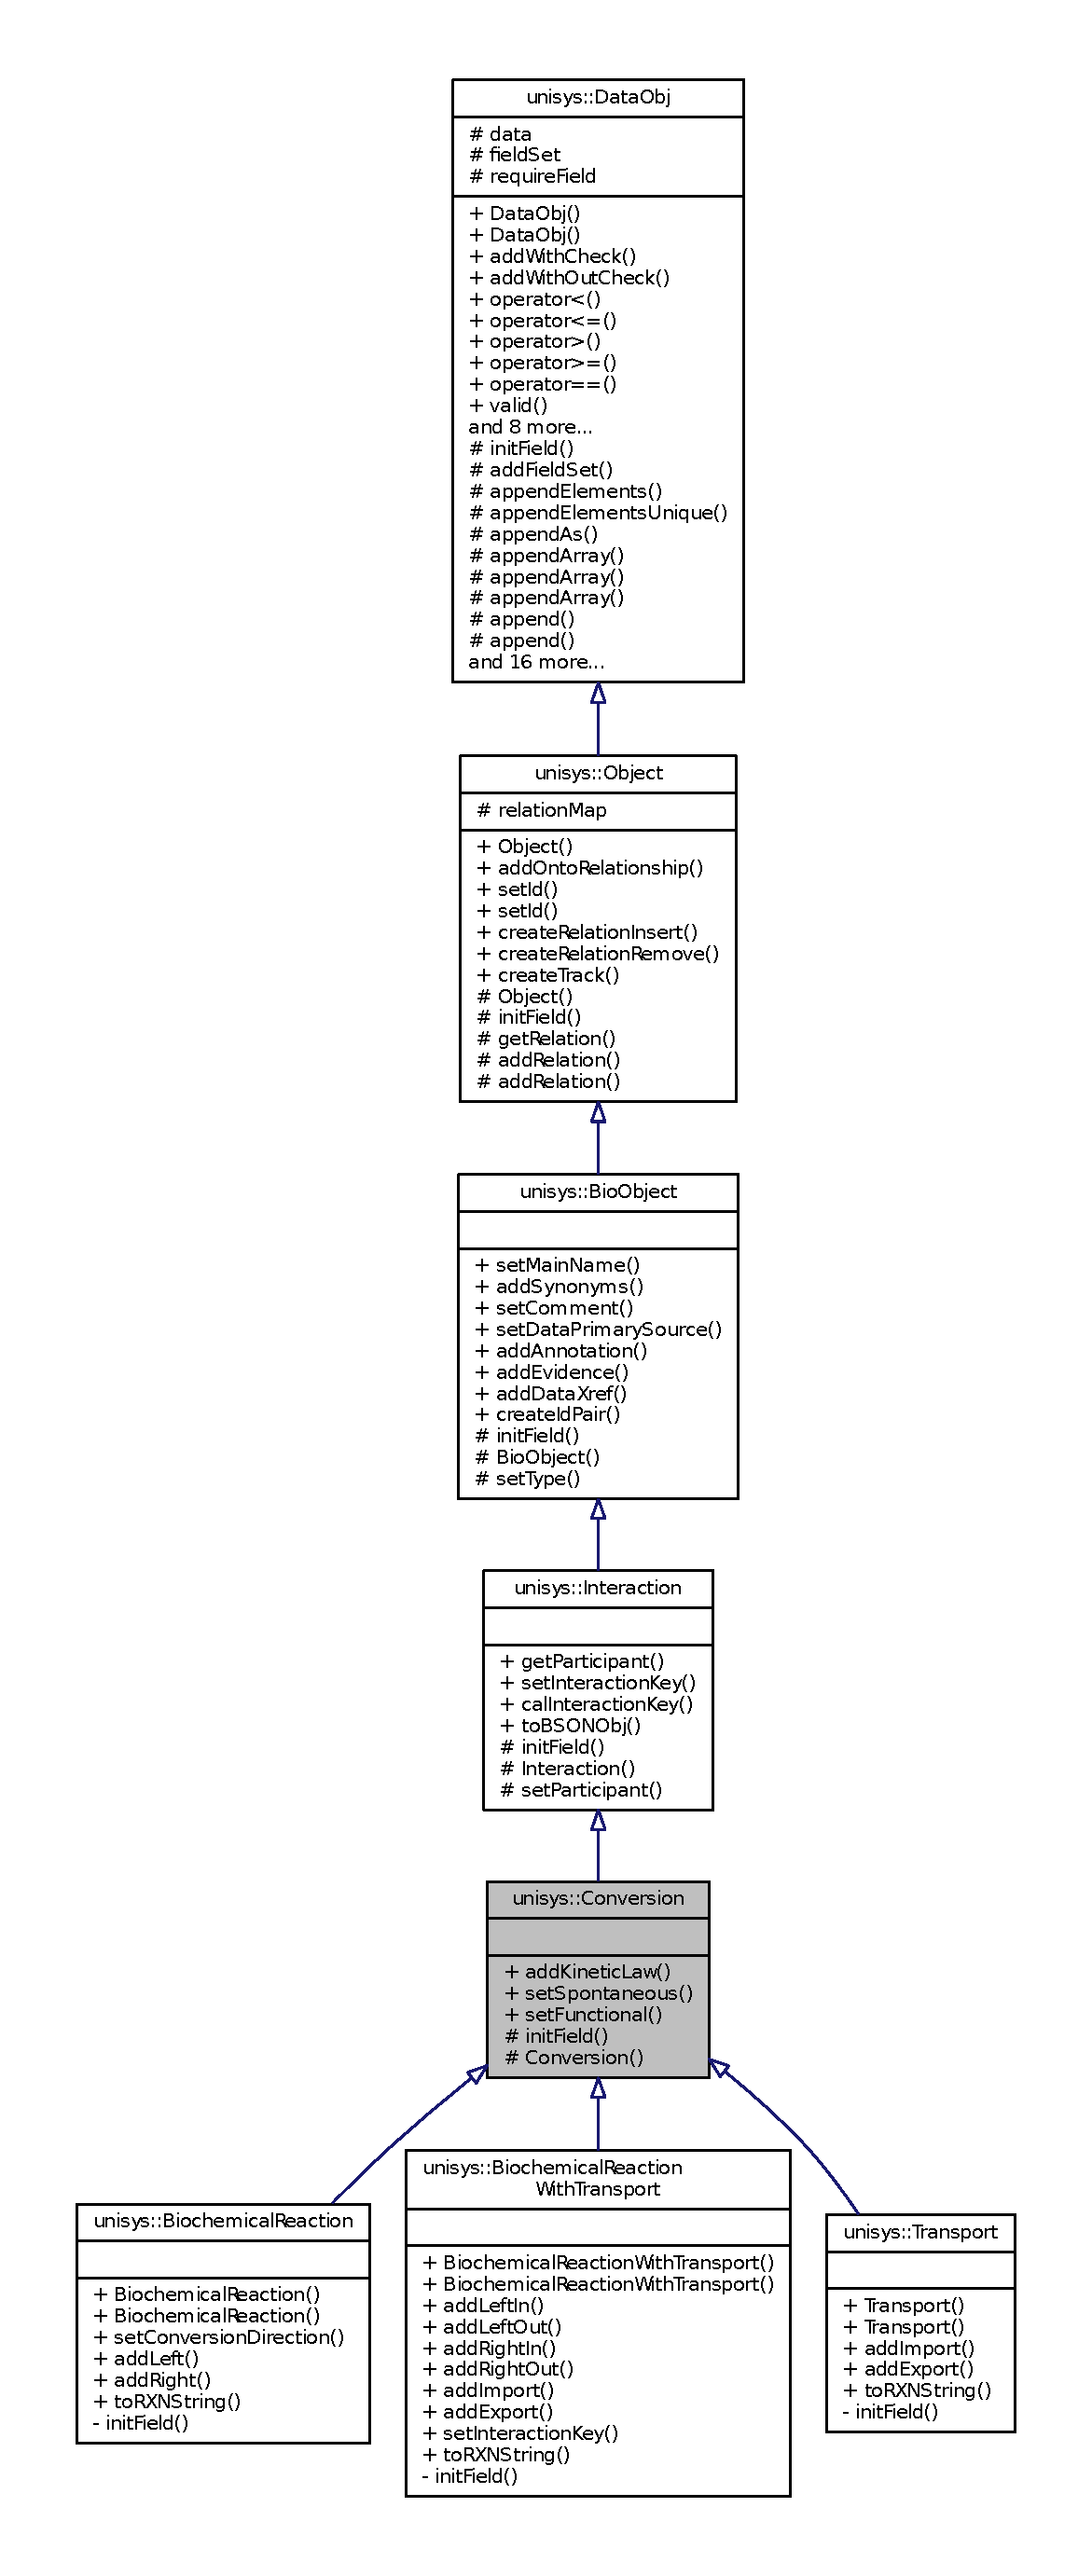
\includegraphics[height=550pt]{classunisys_1_1Conversion__inherit__graph}
\end{center}
\end{figure}


Collaboration diagram for unisys\-:\-:Conversion\-:
\nopagebreak
\begin{figure}[H]
\begin{center}
\leavevmode
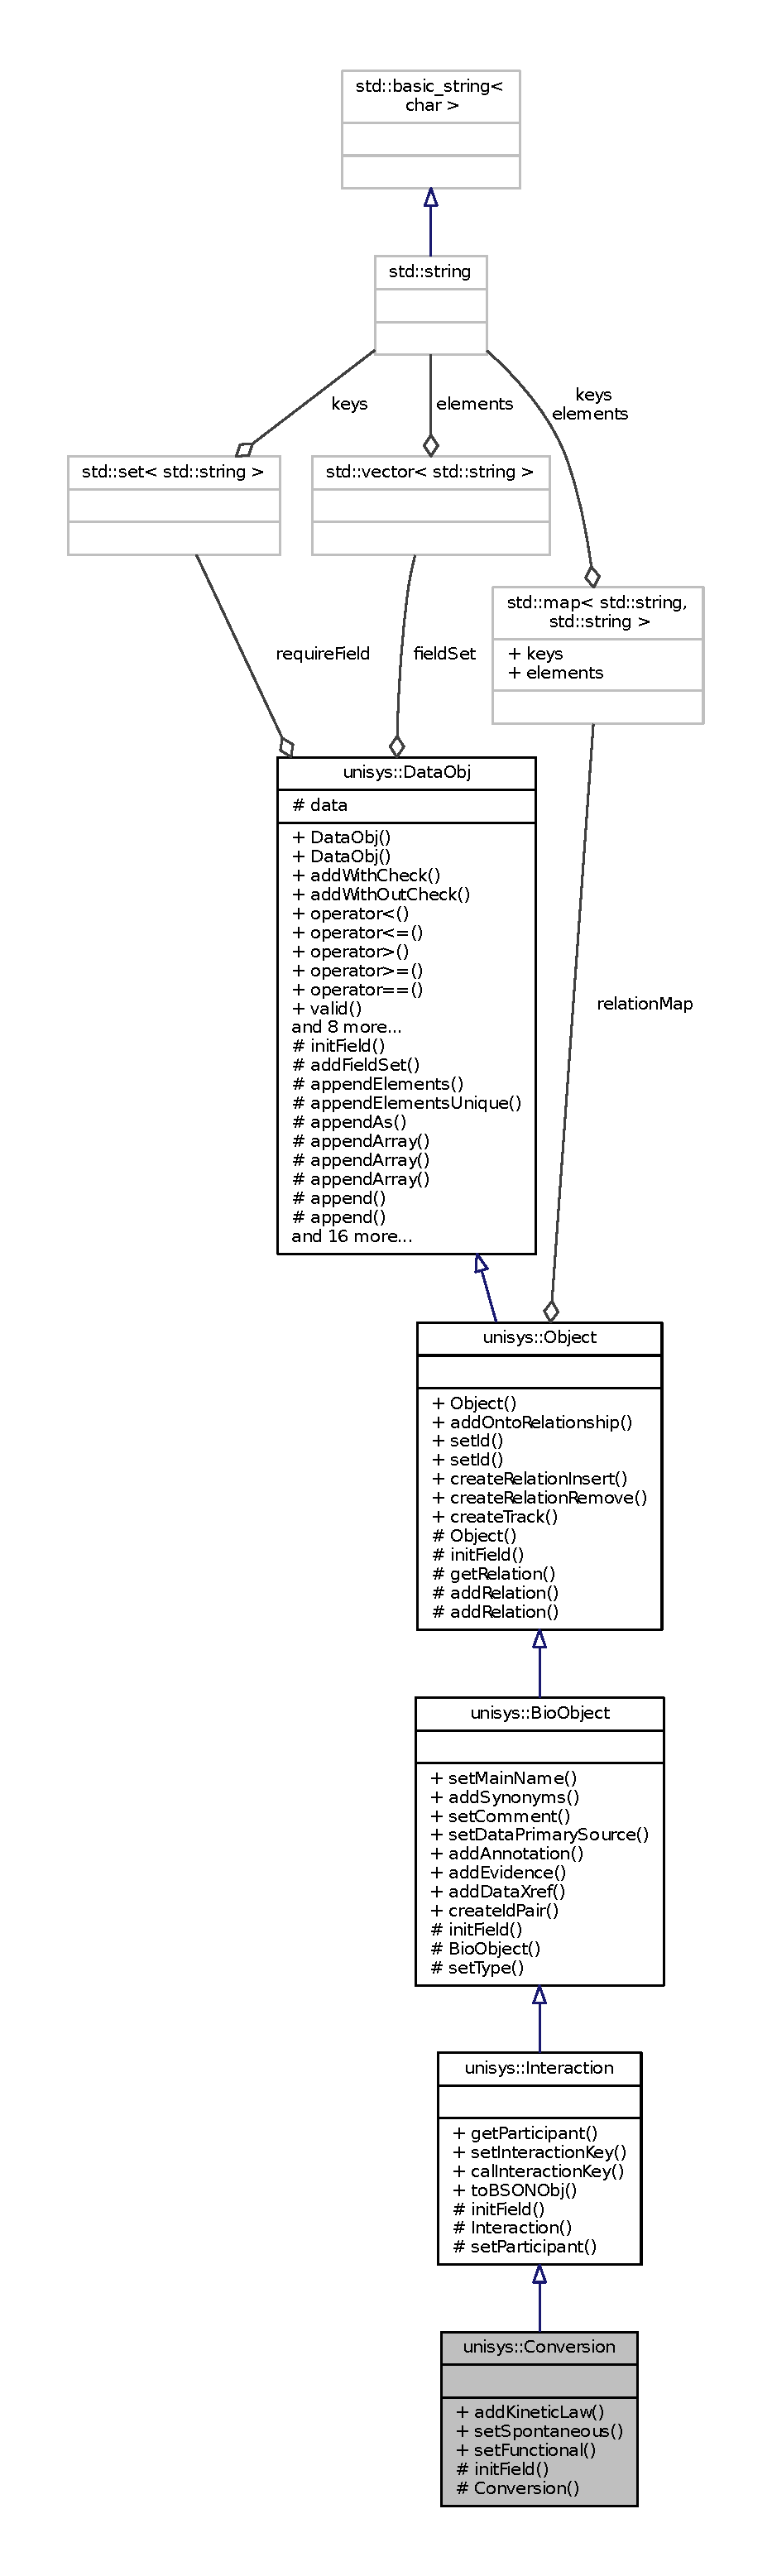
\includegraphics[height=550pt]{classunisys_1_1Conversion__coll__graph}
\end{center}
\end{figure}
\subsection*{Public Member Functions}
\begin{DoxyCompactItemize}
\item 
void \hyperlink{classunisys_1_1Conversion_afca30f92317873b364fe2a25e194dc04}{add\-Kinetic\-Law} (\hyperlink{classunisys_1_1MathML}{Math\-M\-L} \&kinetic\-Law)
\item 
void \hyperlink{classunisys_1_1Conversion_a7deb28962c5f6ba35dab941585bce610}{set\-Spontaneous} (bool value=true)
\item 
void \hyperlink{classunisys_1_1Conversion_ad845f9c8f2e968f346fc67507f48d565}{set\-Functional} (bool value=true)
\end{DoxyCompactItemize}
\subsection*{Protected Member Functions}
\begin{DoxyCompactItemize}
\item 
void \hyperlink{classunisys_1_1Conversion_adafab2a857d6b15d5e07a0d59f4f6596}{init\-Field} ()
\item 
\hyperlink{classunisys_1_1Conversion_ac70f7803971acc97b3b69b7225eb3c06}{Conversion} ()
\end{DoxyCompactItemize}


\subsection{Detailed Description}
This class is for miriam cross reference annotation. 

\begin{DoxyVerb}        BSON structure:
        {   
            _id: <string>, #madatory
            type: <string>,
            ontologyRelationship: {<RelationshipBOSON>, <RelationshipBOSON>, ...},
            name: {<string>,<string>, ...}
            comment: <string>,
            dataPrimarySource: <XrefBOSON>,
            functionAnnotation: {<AnnotationBOSON>, <AnnotationBOSON>, ...},
            evidence: {<EvidenceBOSON>, <EvidenceBOSON>, ...},
            dataxref: {<XrefBOSON>, <XrefBOSON>, ...},
            participant: {<StoichiometryBOSON>, <StoichiometryBOSON>, ...},
            interactionKey: <string>,
            conversionDirection: <DbRef>,
            kineticLaw: {<MathMLBOSON>, <MathMLBOSON>, ...}
            spontaneous: <string>,
            functional: <string>
        }\end{DoxyVerb}
 

\subsection{Constructor \& Destructor Documentation}
\hypertarget{classunisys_1_1Conversion_ac70f7803971acc97b3b69b7225eb3c06}{\index{unisys\-::\-Conversion@{unisys\-::\-Conversion}!Conversion@{Conversion}}
\index{Conversion@{Conversion}!unisys::Conversion@{unisys\-::\-Conversion}}
\subsubsection[{Conversion}]{\setlength{\rightskip}{0pt plus 5cm}unisys\-::\-Conversion\-::\-Conversion (
\begin{DoxyParamCaption}
{}
\end{DoxyParamCaption}
)\hspace{0.3cm}{\ttfamily [protected]}}}\label{classunisys_1_1Conversion_ac70f7803971acc97b3b69b7225eb3c06}


\subsection{Member Function Documentation}
\hypertarget{classunisys_1_1Conversion_afca30f92317873b364fe2a25e194dc04}{\index{unisys\-::\-Conversion@{unisys\-::\-Conversion}!add\-Kinetic\-Law@{add\-Kinetic\-Law}}
\index{add\-Kinetic\-Law@{add\-Kinetic\-Law}!unisys::Conversion@{unisys\-::\-Conversion}}
\subsubsection[{add\-Kinetic\-Law}]{\setlength{\rightskip}{0pt plus 5cm}void unisys\-::\-Conversion\-::add\-Kinetic\-Law (
\begin{DoxyParamCaption}
\item[{{\bf Math\-M\-L} \&}]{kinetic\-Law}
\end{DoxyParamCaption}
)}}\label{classunisys_1_1Conversion_afca30f92317873b364fe2a25e194dc04}
\hypertarget{classunisys_1_1Conversion_adafab2a857d6b15d5e07a0d59f4f6596}{\index{unisys\-::\-Conversion@{unisys\-::\-Conversion}!init\-Field@{init\-Field}}
\index{init\-Field@{init\-Field}!unisys::Conversion@{unisys\-::\-Conversion}}
\subsubsection[{init\-Field}]{\setlength{\rightskip}{0pt plus 5cm}void unisys\-::\-Conversion\-::init\-Field (
\begin{DoxyParamCaption}
{}
\end{DoxyParamCaption}
)\hspace{0.3cm}{\ttfamily [protected]}, {\ttfamily [virtual]}}}\label{classunisys_1_1Conversion_adafab2a857d6b15d5e07a0d59f4f6596}


Reimplemented from \hyperlink{classunisys_1_1Interaction_a84c6c3e09f83ec8dd8dec7485f97e02b}{unisys\-::\-Interaction}.



Reimplemented in \hyperlink{classunisys_1_1BiochemicalReactionWithTransport_a9999c6a5353e9b62056691cf0187f04f}{unisys\-::\-Biochemical\-Reaction\-With\-Transport}, \hyperlink{classunisys_1_1Transport_a04f17e27ff568c45688cde1a95265dea}{unisys\-::\-Transport}, and \hyperlink{classunisys_1_1BiochemicalReaction_a61d5cb519be2ac672ae8e243abdc7489}{unisys\-::\-Biochemical\-Reaction}.

\hypertarget{classunisys_1_1Conversion_ad845f9c8f2e968f346fc67507f48d565}{\index{unisys\-::\-Conversion@{unisys\-::\-Conversion}!set\-Functional@{set\-Functional}}
\index{set\-Functional@{set\-Functional}!unisys::Conversion@{unisys\-::\-Conversion}}
\subsubsection[{set\-Functional}]{\setlength{\rightskip}{0pt plus 5cm}void unisys\-::\-Conversion\-::set\-Functional (
\begin{DoxyParamCaption}
\item[{bool}]{value = {\ttfamily true}}
\end{DoxyParamCaption}
)}}\label{classunisys_1_1Conversion_ad845f9c8f2e968f346fc67507f48d565}
\hypertarget{classunisys_1_1Conversion_a7deb28962c5f6ba35dab941585bce610}{\index{unisys\-::\-Conversion@{unisys\-::\-Conversion}!set\-Spontaneous@{set\-Spontaneous}}
\index{set\-Spontaneous@{set\-Spontaneous}!unisys::Conversion@{unisys\-::\-Conversion}}
\subsubsection[{set\-Spontaneous}]{\setlength{\rightskip}{0pt plus 5cm}void unisys\-::\-Conversion\-::set\-Spontaneous (
\begin{DoxyParamCaption}
\item[{bool}]{value = {\ttfamily true}}
\end{DoxyParamCaption}
)}}\label{classunisys_1_1Conversion_a7deb28962c5f6ba35dab941585bce610}


The documentation for this class was generated from the following file\-:\begin{DoxyCompactItemize}
\item 
\hyperlink{ObjClass_8h}{Obj\-Class.\-h}\end{DoxyCompactItemize}

\hypertarget{classunisys_1_1Database}{\section{unisys\-:\-:Database Class Reference}
\label{classunisys_1_1Database}\index{unisys\-::\-Database@{unisys\-::\-Database}}
}


This class is a database handle class.  




{\ttfamily \#include $<$database.\-h$>$}



Collaboration diagram for unisys\-:\-:Database\-:
\nopagebreak
\begin{figure}[H]
\begin{center}
\leavevmode
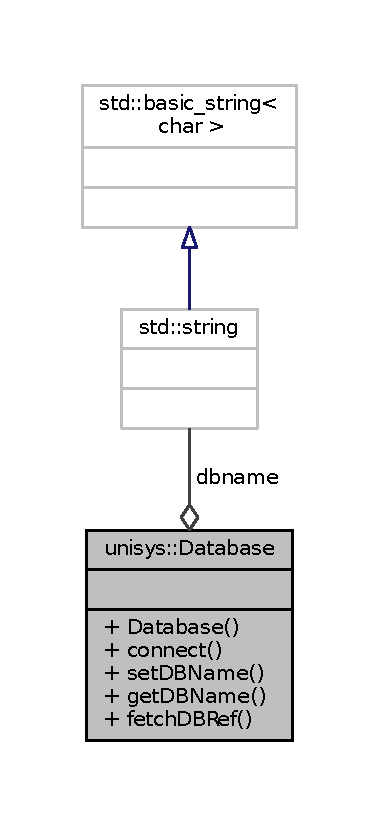
\includegraphics[width=182pt]{classunisys_1_1Database__coll__graph}
\end{center}
\end{figure}
\subsection*{Public Member Functions}
\begin{DoxyCompactItemize}
\item 
\hyperlink{classunisys_1_1Database_a42a97889bb32435bb1ab8b84382a702d}{Database} (std\-::string const \&\hyperlink{classunisys_1_1Database_a0643effdb77f75a9f569a6c1a9aeaf90}{dbname}=\char`\"{}test\char`\"{})
\begin{DoxyCompactList}\small\item\em Overloaded contructor with specific database name. \end{DoxyCompactList}\item 
void \hyperlink{classunisys_1_1Database_a2df5d09f2fef6cb0ed002874fd4bee16}{connect} (std\-::string const \&server\-Hostname)
\begin{DoxyCompactList}\small\item\em Overloaded interface of connection function. \end{DoxyCompactList}\item 
void \hyperlink{classunisys_1_1Database_a842e22d2c0f68e9403ffb3e7d301a6fb}{set\-D\-B\-Name} (std\-::string const \&\hyperlink{classunisys_1_1Database_a0643effdb77f75a9f569a6c1a9aeaf90}{dbname})
\begin{DoxyCompactList}\small\item\em Set or change database name. \end{DoxyCompactList}\item 
std\-::string \hyperlink{classunisys_1_1Database_abf3f6aa38de47f1587163199d6aaae75}{get\-D\-B\-Name} ()
\begin{DoxyCompactList}\small\item\em Return database name. \end{DoxyCompactList}\item 
mongo\-::\-B\-S\-O\-N\-Obj \hyperlink{classunisys_1_1Database_ae87518cd37f1dddbc808e763ad1e9803}{fetch\-D\-B\-Ref} (mongo\-::\-B\-S\-O\-N\-Obj const \&bson\-Obj)  throw (\-Query\-Error)
\begin{DoxyCompactList}\small\item\em Dereference boson database reference (D\-B\-Ref) \end{DoxyCompactList}\end{DoxyCompactItemize}
\subsection*{Private Attributes}
\begin{DoxyCompactItemize}
\item 
std\-::string \hyperlink{classunisys_1_1Database_a0643effdb77f75a9f569a6c1a9aeaf90}{dbname}
\begin{DoxyCompactList}\small\item\em \hyperlink{classunisys_1_1Database}{Database} name, defualt is test. \end{DoxyCompactList}\end{DoxyCompactItemize}
\subsection*{Friends}
\begin{DoxyCompactItemize}
\item 
class \hyperlink{classunisys_1_1Database_a263621696f00d0fefadbd6b1b52da6b5}{Updater}
\end{DoxyCompactItemize}


\subsection{Detailed Description}
This class is a database handle class. 

\hyperlink{classunisys_1_1Database}{Database} class is derived from mongo\-::\-D\-B\-Client\-Connection, used to handle the connection between client and database. In this derived class, there are some functions that specific to Uni\-Sys\-D\-B database data structure. 

\subsection{Constructor \& Destructor Documentation}
\hypertarget{classunisys_1_1Database_a42a97889bb32435bb1ab8b84382a702d}{\index{unisys\-::\-Database@{unisys\-::\-Database}!Database@{Database}}
\index{Database@{Database}!unisys::Database@{unisys\-::\-Database}}
\subsubsection[{Database}]{\setlength{\rightskip}{0pt plus 5cm}unisys\-::\-Database\-::\-Database (
\begin{DoxyParamCaption}
\item[{std\-::string const \&}]{dbname = {\ttfamily \char`\"{}test\char`\"{}}}
\end{DoxyParamCaption}
)}}\label{classunisys_1_1Database_a42a97889bb32435bb1ab8b84382a702d}


Overloaded contructor with specific database name. 



\subsection{Member Function Documentation}
\hypertarget{classunisys_1_1Database_a2df5d09f2fef6cb0ed002874fd4bee16}{\index{unisys\-::\-Database@{unisys\-::\-Database}!connect@{connect}}
\index{connect@{connect}!unisys::Database@{unisys\-::\-Database}}
\subsubsection[{connect}]{\setlength{\rightskip}{0pt plus 5cm}void unisys\-::\-Database\-::connect (
\begin{DoxyParamCaption}
\item[{std\-::string const \&}]{server\-Hostname}
\end{DoxyParamCaption}
)}}\label{classunisys_1_1Database_a2df5d09f2fef6cb0ed002874fd4bee16}


Overloaded interface of connection function. 

\hypertarget{classunisys_1_1Database_ae87518cd37f1dddbc808e763ad1e9803}{\index{unisys\-::\-Database@{unisys\-::\-Database}!fetch\-D\-B\-Ref@{fetch\-D\-B\-Ref}}
\index{fetch\-D\-B\-Ref@{fetch\-D\-B\-Ref}!unisys::Database@{unisys\-::\-Database}}
\subsubsection[{fetch\-D\-B\-Ref}]{\setlength{\rightskip}{0pt plus 5cm}mongo\-::\-B\-S\-O\-N\-Obj unisys\-::\-Database\-::fetch\-D\-B\-Ref (
\begin{DoxyParamCaption}
\item[{mongo\-::\-B\-S\-O\-N\-Obj const \&}]{bson\-Obj}
\end{DoxyParamCaption}
)  throw ({\bf Query\-Error})}}\label{classunisys_1_1Database_ae87518cd37f1dddbc808e763ad1e9803}


Dereference boson database reference (D\-B\-Ref) 

This function retreives bson database reference, which format is \{\char`\"{}\$ref\char`\"{}\-: \char`\"{}collection\-N\-S\char`\"{}, \char`\"{}\$id\char`\"{}\-: \char`\"{}id\char`\"{}\mbox{[}, \char`\"{}\$db\char`\"{}\-: \char`\"{}database\-Name\char`\"{}\mbox{]}\}, as an input and searches for the document that has \char`\"{}\-\_\-id\char`\"{} as describe in D\-B\-Ref from specified collection namespace. 
\begin{DoxyParams}{Parameters}
{\em bson\-Obj} & boson object of D\-B\-Ref \\
\hline
\end{DoxyParams}
\hypertarget{classunisys_1_1Database_abf3f6aa38de47f1587163199d6aaae75}{\index{unisys\-::\-Database@{unisys\-::\-Database}!get\-D\-B\-Name@{get\-D\-B\-Name}}
\index{get\-D\-B\-Name@{get\-D\-B\-Name}!unisys::Database@{unisys\-::\-Database}}
\subsubsection[{get\-D\-B\-Name}]{\setlength{\rightskip}{0pt plus 5cm}std\-::string unisys\-::\-Database\-::get\-D\-B\-Name (
\begin{DoxyParamCaption}
{}
\end{DoxyParamCaption}
)}}\label{classunisys_1_1Database_abf3f6aa38de47f1587163199d6aaae75}


Return database name. 

\hypertarget{classunisys_1_1Database_a842e22d2c0f68e9403ffb3e7d301a6fb}{\index{unisys\-::\-Database@{unisys\-::\-Database}!set\-D\-B\-Name@{set\-D\-B\-Name}}
\index{set\-D\-B\-Name@{set\-D\-B\-Name}!unisys::Database@{unisys\-::\-Database}}
\subsubsection[{set\-D\-B\-Name}]{\setlength{\rightskip}{0pt plus 5cm}void unisys\-::\-Database\-::set\-D\-B\-Name (
\begin{DoxyParamCaption}
\item[{std\-::string const \&}]{dbname}
\end{DoxyParamCaption}
)}}\label{classunisys_1_1Database_a842e22d2c0f68e9403ffb3e7d301a6fb}


Set or change database name. 



\subsection{Friends And Related Function Documentation}
\hypertarget{classunisys_1_1Database_a263621696f00d0fefadbd6b1b52da6b5}{\index{unisys\-::\-Database@{unisys\-::\-Database}!Updater@{Updater}}
\index{Updater@{Updater}!unisys::Database@{unisys\-::\-Database}}
\subsubsection[{Updater}]{\setlength{\rightskip}{0pt plus 5cm}friend class {\bf Updater}\hspace{0.3cm}{\ttfamily [friend]}}}\label{classunisys_1_1Database_a263621696f00d0fefadbd6b1b52da6b5}


\subsection{Member Data Documentation}
\hypertarget{classunisys_1_1Database_a0643effdb77f75a9f569a6c1a9aeaf90}{\index{unisys\-::\-Database@{unisys\-::\-Database}!dbname@{dbname}}
\index{dbname@{dbname}!unisys::Database@{unisys\-::\-Database}}
\subsubsection[{dbname}]{\setlength{\rightskip}{0pt plus 5cm}std\-::string unisys\-::\-Database\-::dbname\hspace{0.3cm}{\ttfamily [private]}}}\label{classunisys_1_1Database_a0643effdb77f75a9f569a6c1a9aeaf90}


\hyperlink{classunisys_1_1Database}{Database} name, defualt is test. 



The documentation for this class was generated from the following file\-:\begin{DoxyCompactItemize}
\item 
\hyperlink{database_8h}{database.\-h}\end{DoxyCompactItemize}

\hypertarget{classunisys_1_1DataError}{\section{unisys\-:\-:Data\-Error Class Reference}
\label{classunisys_1_1DataError}\index{unisys\-::\-Data\-Error@{unisys\-::\-Data\-Error}}
}


{\ttfamily \#include $<$exception.\-h$>$}



Inheritance diagram for unisys\-:\-:Data\-Error\-:
\nopagebreak
\begin{figure}[H]
\begin{center}
\leavevmode
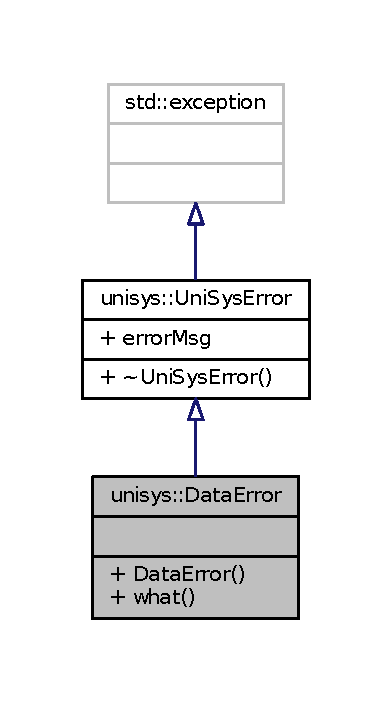
\includegraphics[width=188pt]{classunisys_1_1DataError__inherit__graph}
\end{center}
\end{figure}


Collaboration diagram for unisys\-:\-:Data\-Error\-:
\nopagebreak
\begin{figure}[H]
\begin{center}
\leavevmode
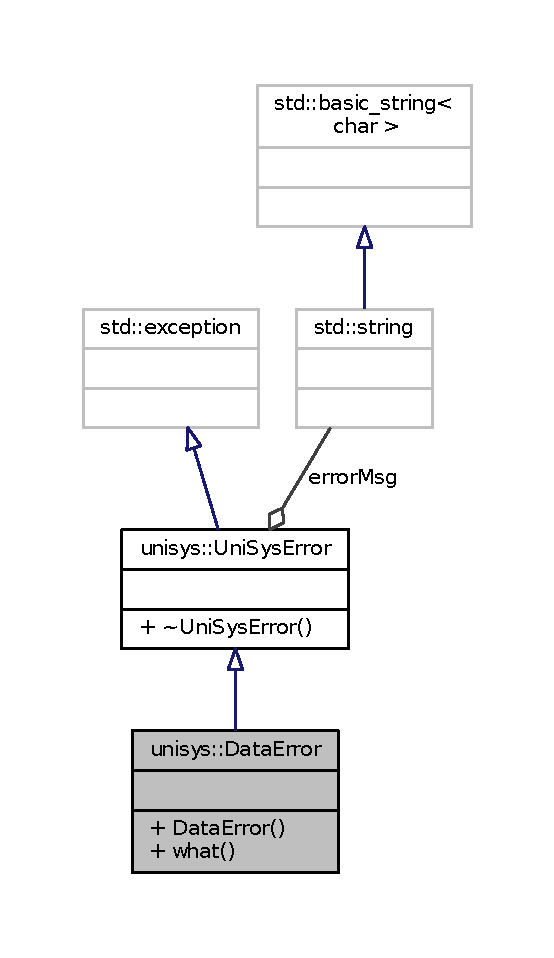
\includegraphics[width=266pt]{classunisys_1_1DataError__coll__graph}
\end{center}
\end{figure}
\subsection*{Public Member Functions}
\begin{DoxyCompactItemize}
\item 
\hyperlink{classunisys_1_1DataError_aea116f4cbfae24addb2bfee7a93f7be4}{Data\-Error} (std\-::string const \&str)
\item 
virtual const char $\ast$ \hyperlink{classunisys_1_1DataError_a0f940955c34f4b741077f781b4ac5d6b}{what} () const   throw ()
\end{DoxyCompactItemize}
\subsection*{Additional Inherited Members}


\subsection{Constructor \& Destructor Documentation}
\hypertarget{classunisys_1_1DataError_aea116f4cbfae24addb2bfee7a93f7be4}{\index{unisys\-::\-Data\-Error@{unisys\-::\-Data\-Error}!Data\-Error@{Data\-Error}}
\index{Data\-Error@{Data\-Error}!unisys::DataError@{unisys\-::\-Data\-Error}}
\subsubsection[{Data\-Error}]{\setlength{\rightskip}{0pt plus 5cm}unisys\-::\-Data\-Error\-::\-Data\-Error (
\begin{DoxyParamCaption}
\item[{std\-::string const \&}]{str}
\end{DoxyParamCaption}
)\hspace{0.3cm}{\ttfamily [inline]}}}\label{classunisys_1_1DataError_aea116f4cbfae24addb2bfee7a93f7be4}


\subsection{Member Function Documentation}
\hypertarget{classunisys_1_1DataError_a0f940955c34f4b741077f781b4ac5d6b}{\index{unisys\-::\-Data\-Error@{unisys\-::\-Data\-Error}!what@{what}}
\index{what@{what}!unisys::DataError@{unisys\-::\-Data\-Error}}
\subsubsection[{what}]{\setlength{\rightskip}{0pt plus 5cm}virtual const char$\ast$ unisys\-::\-Data\-Error\-::what (
\begin{DoxyParamCaption}
{}
\end{DoxyParamCaption}
) const  throw ()\hspace{0.3cm}{\ttfamily [inline]}, {\ttfamily [virtual]}}}\label{classunisys_1_1DataError_a0f940955c34f4b741077f781b4ac5d6b}


The documentation for this class was generated from the following file\-:\begin{DoxyCompactItemize}
\item 
\hyperlink{exception_8h}{exception.\-h}\end{DoxyCompactItemize}

\hypertarget{classunisys_1_1DataObj}{\section{unisys\-:\-:Data\-Obj Class Reference}
\label{classunisys_1_1DataObj}\index{unisys\-::\-Data\-Obj@{unisys\-::\-Data\-Obj}}
}


{\ttfamily \#include $<$D\-B\-Class.\-h$>$}



Inheritance diagram for unisys\-:\-:Data\-Obj\-:
\nopagebreak
\begin{figure}[H]
\begin{center}
\leavevmode
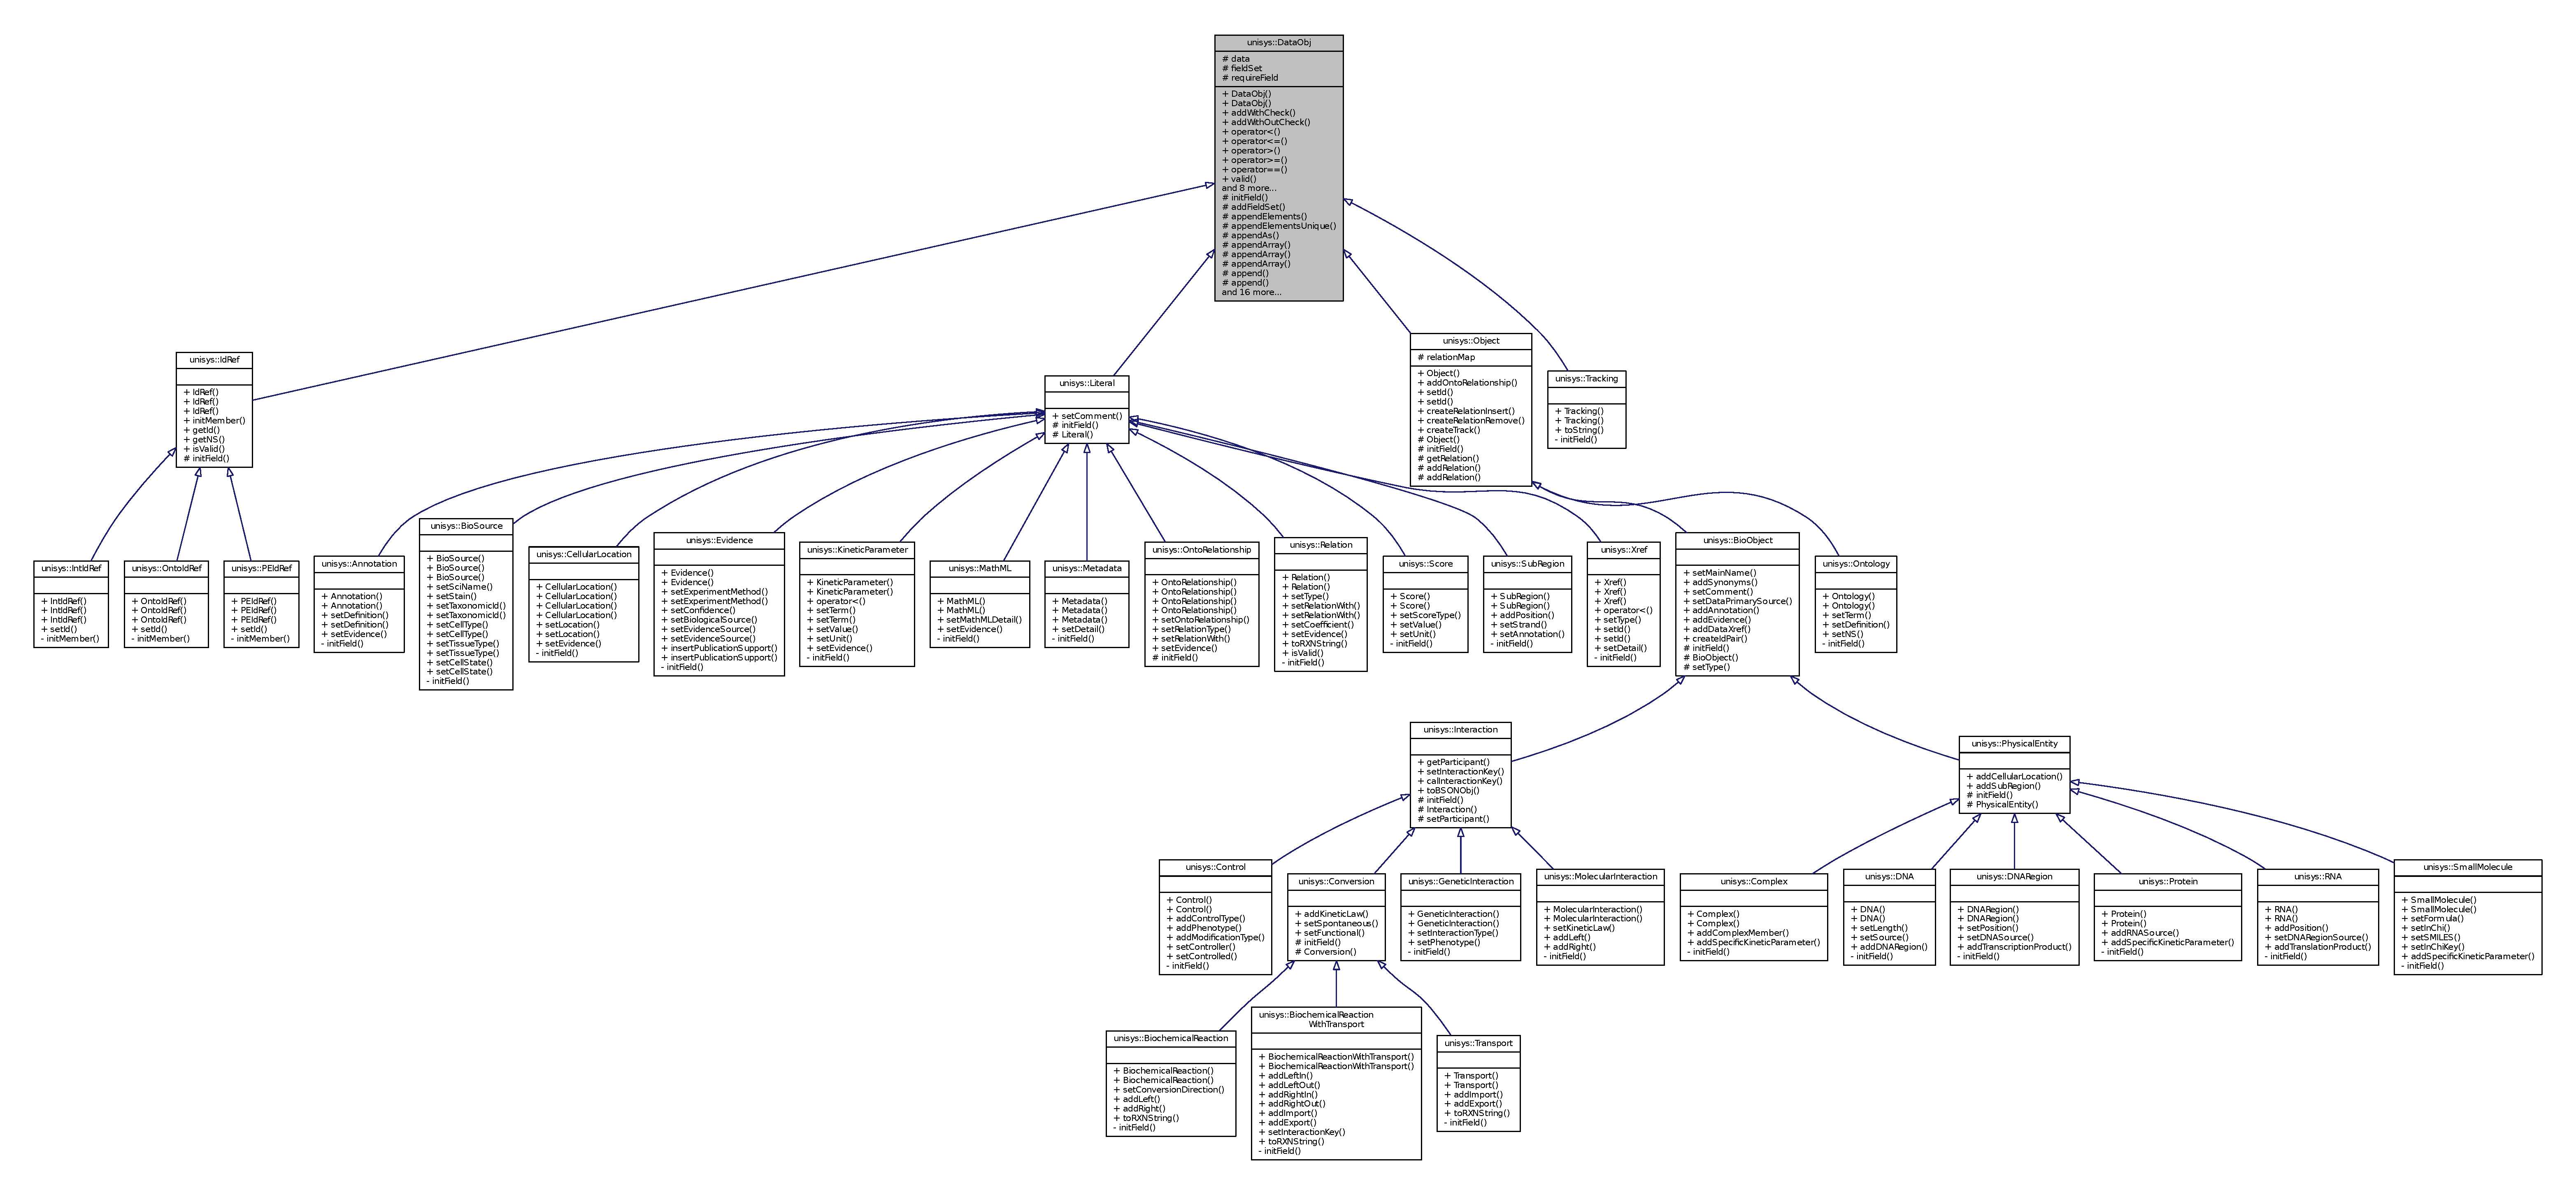
\includegraphics[width=350pt]{classunisys_1_1DataObj__inherit__graph}
\end{center}
\end{figure}


Collaboration diagram for unisys\-:\-:Data\-Obj\-:
\nopagebreak
\begin{figure}[H]
\begin{center}
\leavevmode
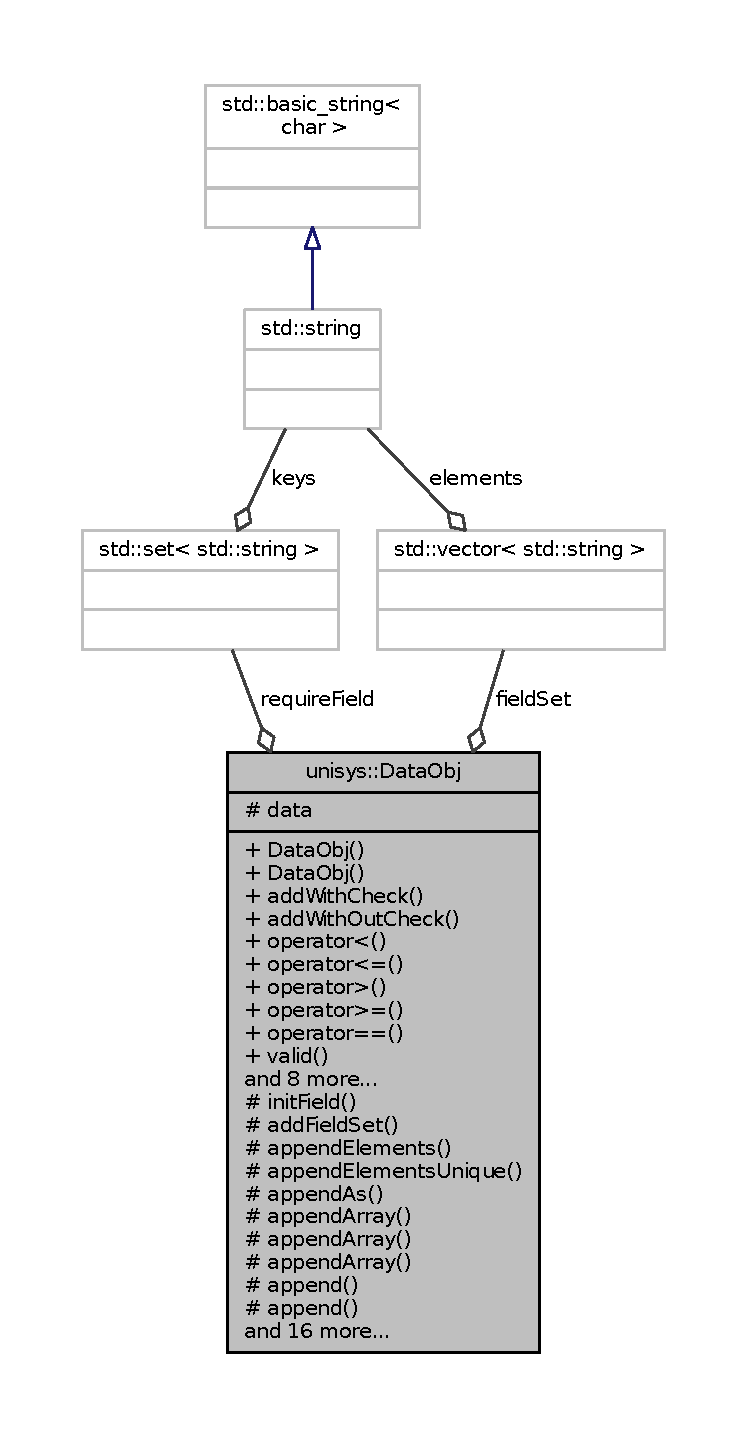
\includegraphics[height=550pt]{classunisys_1_1DataObj__coll__graph}
\end{center}
\end{figure}
\subsection*{Public Member Functions}
\begin{DoxyCompactItemize}
\item 
\hyperlink{classunisys_1_1DataObj_a4d237aaadda27adda13c026e0fdc944e}{Data\-Obj} ()
\item 
\hyperlink{classunisys_1_1DataObj_ab6c5ea140ad5abe24f6dfcbf40176b25}{Data\-Obj} (mongo\-::\-B\-S\-O\-N\-Obj const \&bson\-Obj)
\item 
void \hyperlink{classunisys_1_1DataObj_a3b0243f24755d8ce190486e1c552c6ac}{add\-With\-Check} (mongo\-::\-B\-S\-O\-N\-Obj const \&bson\-Obj)
\item 
void \hyperlink{classunisys_1_1DataObj_a53cfd20ae94853de0407d8328e0eb4fb}{add\-With\-Out\-Check} (mongo\-::\-B\-S\-O\-N\-Obj const \&bson\-Obj)
\item 
bool \hyperlink{classunisys_1_1DataObj_adcbef6f39839328f235674bf10d4309c}{operator$<$} (\hyperlink{classunisys_1_1DataObj}{Data\-Obj} const \&other) const 
\item 
bool \hyperlink{classunisys_1_1DataObj_ab9a18d2b433bff7b1e5bea4bd5fb6090}{operator$<$=} (\hyperlink{classunisys_1_1DataObj}{Data\-Obj} const \&other) const 
\item 
bool \hyperlink{classunisys_1_1DataObj_a13b1c6af9106e32172c7fb3099bd627f}{operator$>$} (\hyperlink{classunisys_1_1DataObj}{Data\-Obj} const \&other) const 
\item 
bool \hyperlink{classunisys_1_1DataObj_acbe081c6f2b2d5531df234619880c090}{operator$>$=} (\hyperlink{classunisys_1_1DataObj}{Data\-Obj} const \&other) const 
\item 
bool \hyperlink{classunisys_1_1DataObj_ad737e7dd24ebf6fd2d77bd42183ab528}{operator==} (\hyperlink{classunisys_1_1DataObj}{Data\-Obj} const \&other) const 
\item 
bool \hyperlink{classunisys_1_1DataObj_a6e4042307576dc0ac8281819402bc250}{valid} () const 
\item 
std\-::string \hyperlink{classunisys_1_1DataObj_aa328fe2b63c53f761529723ad2e45406}{md5} ()
\item 
mongo\-::\-B\-S\-O\-N\-Obj \hyperlink{classunisys_1_1DataObj_ad79e34931486ad2a44b735243e8556d7}{to\-B\-S\-O\-N\-Obj} ()
\item 
std\-::string \hyperlink{classunisys_1_1DataObj_a7c1d7c36a04fdf4d0de279dc57868b0d}{to\-String} (bool is\-Array=false, bool full=false)
\item 
mongo\-::\-B\-S\-O\-N\-Element \hyperlink{classunisys_1_1DataObj_af1e6244874e9120be943641ab566fb14}{get\-Field} (std\-::string const \&field\-Name) const 
\item 
bool \hyperlink{classunisys_1_1DataObj_afd18419bac2fddc4832c24e9e064d7df}{has\-Field} (std\-::string const \&field\-Name) const 
\item 
void \hyperlink{classunisys_1_1DataObj_ab7fdf0a4684987c6e08c82c495065e28}{remove\-Field} (std\-::string const \&field\-Name)
\item 
bool \hyperlink{classunisys_1_1DataObj_ad453f6c376abd5c49fdc05e43def437b}{is\-Owned} () const 
\item 
bool \hyperlink{classunisys_1_1DataObj_af0522a53b0cbc2399c82140da8808212}{is\-Valid} () const 
\end{DoxyCompactItemize}
\subsection*{Protected Member Functions}
\begin{DoxyCompactItemize}
\item 
virtual void \hyperlink{classunisys_1_1DataObj_acdc1989300995834a6c8ff03dc2f1268}{init\-Field} ()=0
\item 
void \hyperlink{classunisys_1_1DataObj_a9a6de9a55343929343fcbba6ac0cbd7f}{add\-Field\-Set} (std\-::string const \&\hyperlink{classunisys_1_1DataObj_a821fe7b1d5c081703b92bba388f8de6f}{field\-Set}, bool is\-Require=false)
\item 
void \hyperlink{classunisys_1_1DataObj_aeae53e9f475d1d5baeacfb17f76d4daf}{append\-Elements} (mongo\-::\-B\-S\-O\-N\-Obj x)
\item 
void \hyperlink{classunisys_1_1DataObj_a6ea78a908761eedba5f944d644c951b3}{append\-Elements\-Unique} (mongo\-::\-B\-S\-O\-N\-Obj x)
\item 
void \hyperlink{classunisys_1_1DataObj_ab1170cf2eb665d6caa1da03ee3cb16bd}{append\-As} (mongo\-::\-B\-S\-O\-N\-Element const \&e, std\-::string const \&field\-Name, bool substitute=false)
\item 
void \hyperlink{classunisys_1_1DataObj_a674e261874099b4a1d1a8ec3204010da}{append\-Array} (std\-::string const \&field\-Name, mongo\-::\-B\-S\-O\-N\-Obj const \&sub\-Obj)
\item 
void \hyperlink{classunisys_1_1DataObj_a7f66c4be5b17528ebab7025c5ad05895}{append\-Array} (std\-::string const \&field\-Name, int start, int stop)
\item 
{\footnotesize template$<$class type $>$ }\\void \hyperlink{classunisys_1_1DataObj_ab14bb36e1a267ea1cfc70eef456995e6}{append\-Array} (std\-::string const \&field\-Name, type const \&sub\-Obj)
\item 
void \hyperlink{classunisys_1_1DataObj_a26834076eef0ce5f207c9b8378fabe3b}{append} (std\-::string const \&field\-Name, const char $\ast$str, int sz, bool substitute=false)
\item 
{\footnotesize template$<$class my\-Type $>$ }\\void \hyperlink{classunisys_1_1DataObj_a2e03be1975e5773b3cecb2dfff81c041}{append} (std\-::string const \&field\-Name, my\-Type value, bool substitute=false)
\item 
void \hyperlink{classunisys_1_1DataObj_ab3952fdef2b7b3311d697e0308da79e0}{set} (std\-::string const \&field\-Name, std\-::string const \&value)
\item 
{\footnotesize template$<$class my\-Type $>$ }\\void \hyperlink{classunisys_1_1DataObj_ab41848078c60f0b343f5edc979d12039}{set} (std\-::string const \&field\-Name, my\-Type value)
\item 
void \hyperlink{classunisys_1_1DataObj_ae93e8390d583c6d3588fa8daf56e0b9e}{set} (std\-::string const \&field\-Name, int value)
\item 
void \hyperlink{classunisys_1_1DataObj_a8c21679bf7fb8575279ceb2f7a921976}{set} (std\-::string const \&field\-Name, double value)
\item 
void \hyperlink{classunisys_1_1DataObj_a3c4a277d0e90de7d13b88c7c14d0a99f}{set} (std\-::string const \&field\-Name, const char $\ast$value)
\item 
void \hyperlink{classunisys_1_1DataObj_a853d760d10b49243b7c83b1692d12dbc}{set} (std\-::string const \&field\-Name, bool value)
\item 
void \hyperlink{classunisys_1_1DataObj_a7c2d6a896ed5cdbf5c31aff3691a14a0}{set} (std\-::string const \&field\-Name, int start, int stop)
\item 
void \hyperlink{classunisys_1_1DataObj_a85ef5bce61421b55f16054dc0d8e3ccc}{append\-Time\-T} (std\-::string const \&field\-Name, time\-\_\-t dt, bool substitute=false)
\item 
void \hyperlink{classunisys_1_1DataObj_a66a85f06432cb3b5079bc4dc867ffd47}{append\-Regex} (std\-::string const \&field\-Name, std\-::string const \&regex, std\-::string const \&options=\char`\"{}\char`\"{}, bool substitute=false)
\item 
void \hyperlink{classunisys_1_1DataObj_aee9b67bba224472d199c0327306bffaa}{append\-Time\-Stamp} (std\-::string const \&field\-Name, bool substitute=false)
\item 
void \hyperlink{classunisys_1_1DataObj_a92854b00b01ce8ccdbc2e4b272d2977b}{append\-As\-Number} (std\-::string const \&field\-Name, std\-::string const \&\hyperlink{classunisys_1_1DataObj_a1c5410a047ff8cf88f810a6e3a1a7c29}{data}, bool substitute=false)
\item 
void \hyperlink{classunisys_1_1DataObj_a1ab8b5a73b228a328bbf032d13af43ab}{append\-Null} (std\-::string const \&field\-Name, bool substitute=false)
\item 
void \hyperlink{classunisys_1_1DataObj_a0c23d2edaffd7262391e58251d772f15}{append\-Code} (std\-::string const \&field\-Name, std\-::string const \&code, bool substitute=false)
\item 
void \hyperlink{classunisys_1_1DataObj_ab7582c0c47c4e2d8dbbe8bfcbe9b27c8}{append\-D\-B\-Ref} (std\-::string const \&field\-Name, std\-::string const \&ns, mongo\-::\-O\-I\-D const \&oid, bool substitute=false)
\item 
void \hyperlink{classunisys_1_1DataObj_a0e00b9d4961b2b11eba162a8d2636002}{gen\-O\-I\-D} ()
\item 
void \hyperlink{classunisys_1_1DataObj_aeeae93641245fa30a55aa07d24d44afd}{sort} ()
\end{DoxyCompactItemize}
\subsection*{Protected Attributes}
\begin{DoxyCompactItemize}
\item 
mongo\-::\-B\-S\-O\-N\-Obj \hyperlink{classunisys_1_1DataObj_a1c5410a047ff8cf88f810a6e3a1a7c29}{data}
\item 
std\-::vector$<$ std\-::string $>$ \hyperlink{classunisys_1_1DataObj_a821fe7b1d5c081703b92bba388f8de6f}{field\-Set}
\item 
std\-::set$<$ std\-::string $>$ \hyperlink{classunisys_1_1DataObj_a0edcaa1c3d03422dca7171c32fcf1951}{require\-Field}
\end{DoxyCompactItemize}


\subsection{Constructor \& Destructor Documentation}
\hypertarget{classunisys_1_1DataObj_a4d237aaadda27adda13c026e0fdc944e}{\index{unisys\-::\-Data\-Obj@{unisys\-::\-Data\-Obj}!Data\-Obj@{Data\-Obj}}
\index{Data\-Obj@{Data\-Obj}!unisys::DataObj@{unisys\-::\-Data\-Obj}}
\subsubsection[{Data\-Obj}]{\setlength{\rightskip}{0pt plus 5cm}unisys\-::\-Data\-Obj\-::\-Data\-Obj (
\begin{DoxyParamCaption}
{}
\end{DoxyParamCaption}
)}}\label{classunisys_1_1DataObj_a4d237aaadda27adda13c026e0fdc944e}
\hypertarget{classunisys_1_1DataObj_ab6c5ea140ad5abe24f6dfcbf40176b25}{\index{unisys\-::\-Data\-Obj@{unisys\-::\-Data\-Obj}!Data\-Obj@{Data\-Obj}}
\index{Data\-Obj@{Data\-Obj}!unisys::DataObj@{unisys\-::\-Data\-Obj}}
\subsubsection[{Data\-Obj}]{\setlength{\rightskip}{0pt plus 5cm}unisys\-::\-Data\-Obj\-::\-Data\-Obj (
\begin{DoxyParamCaption}
\item[{mongo\-::\-B\-S\-O\-N\-Obj const \&}]{bson\-Obj}
\end{DoxyParamCaption}
)}}\label{classunisys_1_1DataObj_ab6c5ea140ad5abe24f6dfcbf40176b25}


\subsection{Member Function Documentation}
\hypertarget{classunisys_1_1DataObj_a9a6de9a55343929343fcbba6ac0cbd7f}{\index{unisys\-::\-Data\-Obj@{unisys\-::\-Data\-Obj}!add\-Field\-Set@{add\-Field\-Set}}
\index{add\-Field\-Set@{add\-Field\-Set}!unisys::DataObj@{unisys\-::\-Data\-Obj}}
\subsubsection[{add\-Field\-Set}]{\setlength{\rightskip}{0pt plus 5cm}void unisys\-::\-Data\-Obj\-::add\-Field\-Set (
\begin{DoxyParamCaption}
\item[{std\-::string const \&}]{field\-Set, }
\item[{bool}]{is\-Require = {\ttfamily false}}
\end{DoxyParamCaption}
)\hspace{0.3cm}{\ttfamily [inline]}, {\ttfamily [protected]}}}\label{classunisys_1_1DataObj_a9a6de9a55343929343fcbba6ac0cbd7f}
\hypertarget{classunisys_1_1DataObj_a3b0243f24755d8ce190486e1c552c6ac}{\index{unisys\-::\-Data\-Obj@{unisys\-::\-Data\-Obj}!add\-With\-Check@{add\-With\-Check}}
\index{add\-With\-Check@{add\-With\-Check}!unisys::DataObj@{unisys\-::\-Data\-Obj}}
\subsubsection[{add\-With\-Check}]{\setlength{\rightskip}{0pt plus 5cm}void unisys\-::\-Data\-Obj\-::add\-With\-Check (
\begin{DoxyParamCaption}
\item[{mongo\-::\-B\-S\-O\-N\-Obj const \&}]{bson\-Obj}
\end{DoxyParamCaption}
)}}\label{classunisys_1_1DataObj_a3b0243f24755d8ce190486e1c552c6ac}
\hypertarget{classunisys_1_1DataObj_a53cfd20ae94853de0407d8328e0eb4fb}{\index{unisys\-::\-Data\-Obj@{unisys\-::\-Data\-Obj}!add\-With\-Out\-Check@{add\-With\-Out\-Check}}
\index{add\-With\-Out\-Check@{add\-With\-Out\-Check}!unisys::DataObj@{unisys\-::\-Data\-Obj}}
\subsubsection[{add\-With\-Out\-Check}]{\setlength{\rightskip}{0pt plus 5cm}void unisys\-::\-Data\-Obj\-::add\-With\-Out\-Check (
\begin{DoxyParamCaption}
\item[{mongo\-::\-B\-S\-O\-N\-Obj const \&}]{bson\-Obj}
\end{DoxyParamCaption}
)}}\label{classunisys_1_1DataObj_a53cfd20ae94853de0407d8328e0eb4fb}
\hypertarget{classunisys_1_1DataObj_a26834076eef0ce5f207c9b8378fabe3b}{\index{unisys\-::\-Data\-Obj@{unisys\-::\-Data\-Obj}!append@{append}}
\index{append@{append}!unisys::DataObj@{unisys\-::\-Data\-Obj}}
\subsubsection[{append}]{\setlength{\rightskip}{0pt plus 5cm}void unisys\-::\-Data\-Obj\-::append (
\begin{DoxyParamCaption}
\item[{std\-::string const \&}]{field\-Name, }
\item[{const char $\ast$}]{str, }
\item[{int}]{sz, }
\item[{bool}]{substitute = {\ttfamily false}}
\end{DoxyParamCaption}
)\hspace{0.3cm}{\ttfamily [protected]}}}\label{classunisys_1_1DataObj_a26834076eef0ce5f207c9b8378fabe3b}
\hypertarget{classunisys_1_1DataObj_a2e03be1975e5773b3cecb2dfff81c041}{\index{unisys\-::\-Data\-Obj@{unisys\-::\-Data\-Obj}!append@{append}}
\index{append@{append}!unisys::DataObj@{unisys\-::\-Data\-Obj}}
\subsubsection[{append}]{\setlength{\rightskip}{0pt plus 5cm}template$<$class my\-Type $>$ void unisys\-::\-Data\-Obj\-::append (
\begin{DoxyParamCaption}
\item[{std\-::string const \&}]{field\-Name, }
\item[{my\-Type}]{value, }
\item[{bool}]{substitute = {\ttfamily false}}
\end{DoxyParamCaption}
)\hspace{0.3cm}{\ttfamily [inline]}, {\ttfamily [protected]}}}\label{classunisys_1_1DataObj_a2e03be1975e5773b3cecb2dfff81c041}
\hypertarget{classunisys_1_1DataObj_a674e261874099b4a1d1a8ec3204010da}{\index{unisys\-::\-Data\-Obj@{unisys\-::\-Data\-Obj}!append\-Array@{append\-Array}}
\index{append\-Array@{append\-Array}!unisys::DataObj@{unisys\-::\-Data\-Obj}}
\subsubsection[{append\-Array}]{\setlength{\rightskip}{0pt plus 5cm}void unisys\-::\-Data\-Obj\-::append\-Array (
\begin{DoxyParamCaption}
\item[{std\-::string const \&}]{field\-Name, }
\item[{mongo\-::\-B\-S\-O\-N\-Obj const \&}]{sub\-Obj}
\end{DoxyParamCaption}
)\hspace{0.3cm}{\ttfamily [protected]}}}\label{classunisys_1_1DataObj_a674e261874099b4a1d1a8ec3204010da}
\hypertarget{classunisys_1_1DataObj_a7f66c4be5b17528ebab7025c5ad05895}{\index{unisys\-::\-Data\-Obj@{unisys\-::\-Data\-Obj}!append\-Array@{append\-Array}}
\index{append\-Array@{append\-Array}!unisys::DataObj@{unisys\-::\-Data\-Obj}}
\subsubsection[{append\-Array}]{\setlength{\rightskip}{0pt plus 5cm}void unisys\-::\-Data\-Obj\-::append\-Array (
\begin{DoxyParamCaption}
\item[{std\-::string const \&}]{field\-Name, }
\item[{int}]{start, }
\item[{int}]{stop}
\end{DoxyParamCaption}
)\hspace{0.3cm}{\ttfamily [protected]}}}\label{classunisys_1_1DataObj_a7f66c4be5b17528ebab7025c5ad05895}
\hypertarget{classunisys_1_1DataObj_ab14bb36e1a267ea1cfc70eef456995e6}{\index{unisys\-::\-Data\-Obj@{unisys\-::\-Data\-Obj}!append\-Array@{append\-Array}}
\index{append\-Array@{append\-Array}!unisys::DataObj@{unisys\-::\-Data\-Obj}}
\subsubsection[{append\-Array}]{\setlength{\rightskip}{0pt plus 5cm}template$<$class type $>$ void unisys\-::\-Data\-Obj\-::append\-Array (
\begin{DoxyParamCaption}
\item[{std\-::string const \&}]{field\-Name, }
\item[{type const \&}]{sub\-Obj}
\end{DoxyParamCaption}
)\hspace{0.3cm}{\ttfamily [inline]}, {\ttfamily [protected]}}}\label{classunisys_1_1DataObj_ab14bb36e1a267ea1cfc70eef456995e6}
\hypertarget{classunisys_1_1DataObj_ab1170cf2eb665d6caa1da03ee3cb16bd}{\index{unisys\-::\-Data\-Obj@{unisys\-::\-Data\-Obj}!append\-As@{append\-As}}
\index{append\-As@{append\-As}!unisys::DataObj@{unisys\-::\-Data\-Obj}}
\subsubsection[{append\-As}]{\setlength{\rightskip}{0pt plus 5cm}void unisys\-::\-Data\-Obj\-::append\-As (
\begin{DoxyParamCaption}
\item[{mongo\-::\-B\-S\-O\-N\-Element const \&}]{e, }
\item[{std\-::string const \&}]{field\-Name, }
\item[{bool}]{substitute = {\ttfamily false}}
\end{DoxyParamCaption}
)\hspace{0.3cm}{\ttfamily [protected]}}}\label{classunisys_1_1DataObj_ab1170cf2eb665d6caa1da03ee3cb16bd}
\hypertarget{classunisys_1_1DataObj_a92854b00b01ce8ccdbc2e4b272d2977b}{\index{unisys\-::\-Data\-Obj@{unisys\-::\-Data\-Obj}!append\-As\-Number@{append\-As\-Number}}
\index{append\-As\-Number@{append\-As\-Number}!unisys::DataObj@{unisys\-::\-Data\-Obj}}
\subsubsection[{append\-As\-Number}]{\setlength{\rightskip}{0pt plus 5cm}void unisys\-::\-Data\-Obj\-::append\-As\-Number (
\begin{DoxyParamCaption}
\item[{std\-::string const \&}]{field\-Name, }
\item[{std\-::string const \&}]{data, }
\item[{bool}]{substitute = {\ttfamily false}}
\end{DoxyParamCaption}
)\hspace{0.3cm}{\ttfamily [protected]}}}\label{classunisys_1_1DataObj_a92854b00b01ce8ccdbc2e4b272d2977b}
\hypertarget{classunisys_1_1DataObj_a0c23d2edaffd7262391e58251d772f15}{\index{unisys\-::\-Data\-Obj@{unisys\-::\-Data\-Obj}!append\-Code@{append\-Code}}
\index{append\-Code@{append\-Code}!unisys::DataObj@{unisys\-::\-Data\-Obj}}
\subsubsection[{append\-Code}]{\setlength{\rightskip}{0pt plus 5cm}void unisys\-::\-Data\-Obj\-::append\-Code (
\begin{DoxyParamCaption}
\item[{std\-::string const \&}]{field\-Name, }
\item[{std\-::string const \&}]{code, }
\item[{bool}]{substitute = {\ttfamily false}}
\end{DoxyParamCaption}
)\hspace{0.3cm}{\ttfamily [protected]}}}\label{classunisys_1_1DataObj_a0c23d2edaffd7262391e58251d772f15}
\hypertarget{classunisys_1_1DataObj_ab7582c0c47c4e2d8dbbe8bfcbe9b27c8}{\index{unisys\-::\-Data\-Obj@{unisys\-::\-Data\-Obj}!append\-D\-B\-Ref@{append\-D\-B\-Ref}}
\index{append\-D\-B\-Ref@{append\-D\-B\-Ref}!unisys::DataObj@{unisys\-::\-Data\-Obj}}
\subsubsection[{append\-D\-B\-Ref}]{\setlength{\rightskip}{0pt plus 5cm}void unisys\-::\-Data\-Obj\-::append\-D\-B\-Ref (
\begin{DoxyParamCaption}
\item[{std\-::string const \&}]{field\-Name, }
\item[{std\-::string const \&}]{ns, }
\item[{mongo\-::\-O\-I\-D const \&}]{oid, }
\item[{bool}]{substitute = {\ttfamily false}}
\end{DoxyParamCaption}
)\hspace{0.3cm}{\ttfamily [protected]}}}\label{classunisys_1_1DataObj_ab7582c0c47c4e2d8dbbe8bfcbe9b27c8}
\hypertarget{classunisys_1_1DataObj_aeae53e9f475d1d5baeacfb17f76d4daf}{\index{unisys\-::\-Data\-Obj@{unisys\-::\-Data\-Obj}!append\-Elements@{append\-Elements}}
\index{append\-Elements@{append\-Elements}!unisys::DataObj@{unisys\-::\-Data\-Obj}}
\subsubsection[{append\-Elements}]{\setlength{\rightskip}{0pt plus 5cm}void unisys\-::\-Data\-Obj\-::append\-Elements (
\begin{DoxyParamCaption}
\item[{mongo\-::\-B\-S\-O\-N\-Obj}]{x}
\end{DoxyParamCaption}
)\hspace{0.3cm}{\ttfamily [protected]}}}\label{classunisys_1_1DataObj_aeae53e9f475d1d5baeacfb17f76d4daf}
\hypertarget{classunisys_1_1DataObj_a6ea78a908761eedba5f944d644c951b3}{\index{unisys\-::\-Data\-Obj@{unisys\-::\-Data\-Obj}!append\-Elements\-Unique@{append\-Elements\-Unique}}
\index{append\-Elements\-Unique@{append\-Elements\-Unique}!unisys::DataObj@{unisys\-::\-Data\-Obj}}
\subsubsection[{append\-Elements\-Unique}]{\setlength{\rightskip}{0pt plus 5cm}void unisys\-::\-Data\-Obj\-::append\-Elements\-Unique (
\begin{DoxyParamCaption}
\item[{mongo\-::\-B\-S\-O\-N\-Obj}]{x}
\end{DoxyParamCaption}
)\hspace{0.3cm}{\ttfamily [protected]}}}\label{classunisys_1_1DataObj_a6ea78a908761eedba5f944d644c951b3}
\hypertarget{classunisys_1_1DataObj_a1ab8b5a73b228a328bbf032d13af43ab}{\index{unisys\-::\-Data\-Obj@{unisys\-::\-Data\-Obj}!append\-Null@{append\-Null}}
\index{append\-Null@{append\-Null}!unisys::DataObj@{unisys\-::\-Data\-Obj}}
\subsubsection[{append\-Null}]{\setlength{\rightskip}{0pt plus 5cm}void unisys\-::\-Data\-Obj\-::append\-Null (
\begin{DoxyParamCaption}
\item[{std\-::string const \&}]{field\-Name, }
\item[{bool}]{substitute = {\ttfamily false}}
\end{DoxyParamCaption}
)\hspace{0.3cm}{\ttfamily [protected]}}}\label{classunisys_1_1DataObj_a1ab8b5a73b228a328bbf032d13af43ab}
\hypertarget{classunisys_1_1DataObj_a66a85f06432cb3b5079bc4dc867ffd47}{\index{unisys\-::\-Data\-Obj@{unisys\-::\-Data\-Obj}!append\-Regex@{append\-Regex}}
\index{append\-Regex@{append\-Regex}!unisys::DataObj@{unisys\-::\-Data\-Obj}}
\subsubsection[{append\-Regex}]{\setlength{\rightskip}{0pt plus 5cm}void unisys\-::\-Data\-Obj\-::append\-Regex (
\begin{DoxyParamCaption}
\item[{std\-::string const \&}]{field\-Name, }
\item[{std\-::string const \&}]{regex, }
\item[{std\-::string const \&}]{options = {\ttfamily \char`\"{}\char`\"{}}, }
\item[{bool}]{substitute = {\ttfamily false}}
\end{DoxyParamCaption}
)\hspace{0.3cm}{\ttfamily [protected]}}}\label{classunisys_1_1DataObj_a66a85f06432cb3b5079bc4dc867ffd47}
\hypertarget{classunisys_1_1DataObj_aee9b67bba224472d199c0327306bffaa}{\index{unisys\-::\-Data\-Obj@{unisys\-::\-Data\-Obj}!append\-Time\-Stamp@{append\-Time\-Stamp}}
\index{append\-Time\-Stamp@{append\-Time\-Stamp}!unisys::DataObj@{unisys\-::\-Data\-Obj}}
\subsubsection[{append\-Time\-Stamp}]{\setlength{\rightskip}{0pt plus 5cm}void unisys\-::\-Data\-Obj\-::append\-Time\-Stamp (
\begin{DoxyParamCaption}
\item[{std\-::string const \&}]{field\-Name, }
\item[{bool}]{substitute = {\ttfamily false}}
\end{DoxyParamCaption}
)\hspace{0.3cm}{\ttfamily [protected]}}}\label{classunisys_1_1DataObj_aee9b67bba224472d199c0327306bffaa}
\hypertarget{classunisys_1_1DataObj_a85ef5bce61421b55f16054dc0d8e3ccc}{\index{unisys\-::\-Data\-Obj@{unisys\-::\-Data\-Obj}!append\-Time\-T@{append\-Time\-T}}
\index{append\-Time\-T@{append\-Time\-T}!unisys::DataObj@{unisys\-::\-Data\-Obj}}
\subsubsection[{append\-Time\-T}]{\setlength{\rightskip}{0pt plus 5cm}void unisys\-::\-Data\-Obj\-::append\-Time\-T (
\begin{DoxyParamCaption}
\item[{std\-::string const \&}]{field\-Name, }
\item[{time\-\_\-t}]{dt, }
\item[{bool}]{substitute = {\ttfamily false}}
\end{DoxyParamCaption}
)\hspace{0.3cm}{\ttfamily [protected]}}}\label{classunisys_1_1DataObj_a85ef5bce61421b55f16054dc0d8e3ccc}
\hypertarget{classunisys_1_1DataObj_a0e00b9d4961b2b11eba162a8d2636002}{\index{unisys\-::\-Data\-Obj@{unisys\-::\-Data\-Obj}!gen\-O\-I\-D@{gen\-O\-I\-D}}
\index{gen\-O\-I\-D@{gen\-O\-I\-D}!unisys::DataObj@{unisys\-::\-Data\-Obj}}
\subsubsection[{gen\-O\-I\-D}]{\setlength{\rightskip}{0pt plus 5cm}void unisys\-::\-Data\-Obj\-::gen\-O\-I\-D (
\begin{DoxyParamCaption}
{}
\end{DoxyParamCaption}
)\hspace{0.3cm}{\ttfamily [protected]}}}\label{classunisys_1_1DataObj_a0e00b9d4961b2b11eba162a8d2636002}
\hypertarget{classunisys_1_1DataObj_af1e6244874e9120be943641ab566fb14}{\index{unisys\-::\-Data\-Obj@{unisys\-::\-Data\-Obj}!get\-Field@{get\-Field}}
\index{get\-Field@{get\-Field}!unisys::DataObj@{unisys\-::\-Data\-Obj}}
\subsubsection[{get\-Field}]{\setlength{\rightskip}{0pt plus 5cm}mongo\-::\-B\-S\-O\-N\-Element unisys\-::\-Data\-Obj\-::get\-Field (
\begin{DoxyParamCaption}
\item[{std\-::string const \&}]{field\-Name}
\end{DoxyParamCaption}
) const}}\label{classunisys_1_1DataObj_af1e6244874e9120be943641ab566fb14}
\hypertarget{classunisys_1_1DataObj_afd18419bac2fddc4832c24e9e064d7df}{\index{unisys\-::\-Data\-Obj@{unisys\-::\-Data\-Obj}!has\-Field@{has\-Field}}
\index{has\-Field@{has\-Field}!unisys::DataObj@{unisys\-::\-Data\-Obj}}
\subsubsection[{has\-Field}]{\setlength{\rightskip}{0pt plus 5cm}bool unisys\-::\-Data\-Obj\-::has\-Field (
\begin{DoxyParamCaption}
\item[{std\-::string const \&}]{field\-Name}
\end{DoxyParamCaption}
) const}}\label{classunisys_1_1DataObj_afd18419bac2fddc4832c24e9e064d7df}
\hypertarget{classunisys_1_1DataObj_acdc1989300995834a6c8ff03dc2f1268}{\index{unisys\-::\-Data\-Obj@{unisys\-::\-Data\-Obj}!init\-Field@{init\-Field}}
\index{init\-Field@{init\-Field}!unisys::DataObj@{unisys\-::\-Data\-Obj}}
\subsubsection[{init\-Field}]{\setlength{\rightskip}{0pt plus 5cm}virtual void unisys\-::\-Data\-Obj\-::init\-Field (
\begin{DoxyParamCaption}
{}
\end{DoxyParamCaption}
)\hspace{0.3cm}{\ttfamily [protected]}, {\ttfamily [pure virtual]}}}\label{classunisys_1_1DataObj_acdc1989300995834a6c8ff03dc2f1268}


Implemented in \hyperlink{classunisys_1_1BiochemicalReactionWithTransport_a9999c6a5353e9b62056691cf0187f04f}{unisys\-::\-Biochemical\-Reaction\-With\-Transport}, \hyperlink{classunisys_1_1Transport_a04f17e27ff568c45688cde1a95265dea}{unisys\-::\-Transport}, \hyperlink{classunisys_1_1BiochemicalReaction_a61d5cb519be2ac672ae8e243abdc7489}{unisys\-::\-Biochemical\-Reaction}, \hyperlink{classunisys_1_1Conversion_adafab2a857d6b15d5e07a0d59f4f6596}{unisys\-::\-Conversion}, \hyperlink{classunisys_1_1GeneticInteraction_a946b8270db467290f49a050bd29f55d2}{unisys\-::\-Genetic\-Interaction}, \hyperlink{classunisys_1_1MolecularInteraction_a6bae8353e2734eae8345228f7895665e}{unisys\-::\-Molecular\-Interaction}, \hyperlink{classunisys_1_1Control_ab5bd5022b73b81e3fd18af06027213b1}{unisys\-::\-Control}, \hyperlink{classunisys_1_1Interaction_a84c6c3e09f83ec8dd8dec7485f97e02b}{unisys\-::\-Interaction}, \hyperlink{classunisys_1_1Metadata_a5c3596b451d9539846f8f6ed7bfceaf9}{unisys\-::\-Metadata}, \hyperlink{classunisys_1_1Complex_a63e019fcca3e2d919937694678d9ee1f}{unisys\-::\-Complex}, \hyperlink{classunisys_1_1SubRegion_abaff0ecac757200f5e4173a86054927e}{unisys\-::\-Sub\-Region}, \hyperlink{classunisys_1_1Protein_a41d52894afce9bd0f7f047ac560f38cf}{unisys\-::\-Protein}, \hyperlink{classunisys_1_1KineticParameter_a433dff8934423dc18efda6bb44b2f477}{unisys\-::\-Kinetic\-Parameter}, \hyperlink{classunisys_1_1Tracking_ae8e471c1d4effb3c746e654ba1c970ba}{unisys\-::\-Tracking}, \hyperlink{classunisys_1_1MathML_a51e1fc565fb5ad24ca6557a8db6551d0}{unisys\-::\-Math\-M\-L}, \hyperlink{classunisys_1_1RNA_abeb5db8942c0d2ecac49086d50d6e7ab}{unisys\-::\-R\-N\-A}, \hyperlink{classunisys_1_1CellularLocation_a3aa4c3ebf735ecf9672d0986a63b1dfe}{unisys\-::\-Cellular\-Location}, \hyperlink{classunisys_1_1DNARegion_a213d2340cc8f4172e3f220f1fe9883f1}{unisys\-::\-D\-N\-A\-Region}, \hyperlink{classunisys_1_1Relation_a2793345e5ca711cf0f6f8229a4c652ab}{unisys\-::\-Relation}, \hyperlink{classunisys_1_1IdRef_a2f8143648ba349f8a910ee64b10c0829}{unisys\-::\-Id\-Ref}, \hyperlink{classunisys_1_1DNA_aa33eff29fbf57aa7c626999ade40910d}{unisys\-::\-D\-N\-A}, \hyperlink{classunisys_1_1OntoRelationship_a14ed8b86b0cdc55c63e5ea5443e830a3}{unisys\-::\-Onto\-Relationship}, \hyperlink{classunisys_1_1Annotation_a56a0503bd22b05cae674b8d4df046d9e}{unisys\-::\-Annotation}, \hyperlink{classunisys_1_1SmallMolecule_a0f0da371544569163782603ace820d0a}{unisys\-::\-Small\-Molecule}, \hyperlink{classunisys_1_1Evidence_a8ce7e3da30295b98aa095031ef8491bc}{unisys\-::\-Evidence}, \hyperlink{classunisys_1_1PhysicalEntity_ad445727cb6b1c12e954819d8207104e8}{unisys\-::\-Physical\-Entity}, \hyperlink{classunisys_1_1BioSource_a7a4188b6ce6f969d62c6d903d3e27f09}{unisys\-::\-Bio\-Source}, \hyperlink{classunisys_1_1BioObject_a0437fcc7976ff9e8dc5ce77246c06f71}{unisys\-::\-Bio\-Object}, \hyperlink{classunisys_1_1Score_a3fece7415530d4b577fffcb284535c05}{unisys\-::\-Score}, \hyperlink{classunisys_1_1Ontology_a42f1c4257f60144420b1bc9ac128b5cc}{unisys\-::\-Ontology}, \hyperlink{classunisys_1_1Xref_afc94c9013bfe5cec8a474610212cb941}{unisys\-::\-Xref}, \hyperlink{classunisys_1_1Object_ad0a4afaf978d2cca8a6a27506f06138c}{unisys\-::\-Object}, and \hyperlink{classunisys_1_1Literal_a769b8f41e99619d8635f83d18a02bc1f}{unisys\-::\-Literal}.

\hypertarget{classunisys_1_1DataObj_ad453f6c376abd5c49fdc05e43def437b}{\index{unisys\-::\-Data\-Obj@{unisys\-::\-Data\-Obj}!is\-Owned@{is\-Owned}}
\index{is\-Owned@{is\-Owned}!unisys::DataObj@{unisys\-::\-Data\-Obj}}
\subsubsection[{is\-Owned}]{\setlength{\rightskip}{0pt plus 5cm}bool unisys\-::\-Data\-Obj\-::is\-Owned (
\begin{DoxyParamCaption}
{}
\end{DoxyParamCaption}
) const}}\label{classunisys_1_1DataObj_ad453f6c376abd5c49fdc05e43def437b}
\hypertarget{classunisys_1_1DataObj_af0522a53b0cbc2399c82140da8808212}{\index{unisys\-::\-Data\-Obj@{unisys\-::\-Data\-Obj}!is\-Valid@{is\-Valid}}
\index{is\-Valid@{is\-Valid}!unisys::DataObj@{unisys\-::\-Data\-Obj}}
\subsubsection[{is\-Valid}]{\setlength{\rightskip}{0pt plus 5cm}bool unisys\-::\-Data\-Obj\-::is\-Valid (
\begin{DoxyParamCaption}
{}
\end{DoxyParamCaption}
) const}}\label{classunisys_1_1DataObj_af0522a53b0cbc2399c82140da8808212}


Reimplemented in \hyperlink{classunisys_1_1IdRef_a4ab596023020171bceeb2aed8bd529ce}{unisys\-::\-Id\-Ref}.

\hypertarget{classunisys_1_1DataObj_aa328fe2b63c53f761529723ad2e45406}{\index{unisys\-::\-Data\-Obj@{unisys\-::\-Data\-Obj}!md5@{md5}}
\index{md5@{md5}!unisys::DataObj@{unisys\-::\-Data\-Obj}}
\subsubsection[{md5}]{\setlength{\rightskip}{0pt plus 5cm}std\-::string unisys\-::\-Data\-Obj\-::md5 (
\begin{DoxyParamCaption}
{}
\end{DoxyParamCaption}
)}}\label{classunisys_1_1DataObj_aa328fe2b63c53f761529723ad2e45406}
\hypertarget{classunisys_1_1DataObj_adcbef6f39839328f235674bf10d4309c}{\index{unisys\-::\-Data\-Obj@{unisys\-::\-Data\-Obj}!operator$<$@{operator$<$}}
\index{operator$<$@{operator$<$}!unisys::DataObj@{unisys\-::\-Data\-Obj}}
\subsubsection[{operator$<$}]{\setlength{\rightskip}{0pt plus 5cm}bool unisys\-::\-Data\-Obj\-::operator$<$ (
\begin{DoxyParamCaption}
\item[{{\bf Data\-Obj} const \&}]{other}
\end{DoxyParamCaption}
) const}}\label{classunisys_1_1DataObj_adcbef6f39839328f235674bf10d4309c}
\hypertarget{classunisys_1_1DataObj_ab9a18d2b433bff7b1e5bea4bd5fb6090}{\index{unisys\-::\-Data\-Obj@{unisys\-::\-Data\-Obj}!operator$<$=@{operator$<$=}}
\index{operator$<$=@{operator$<$=}!unisys::DataObj@{unisys\-::\-Data\-Obj}}
\subsubsection[{operator$<$=}]{\setlength{\rightskip}{0pt plus 5cm}bool unisys\-::\-Data\-Obj\-::operator$<$= (
\begin{DoxyParamCaption}
\item[{{\bf Data\-Obj} const \&}]{other}
\end{DoxyParamCaption}
) const}}\label{classunisys_1_1DataObj_ab9a18d2b433bff7b1e5bea4bd5fb6090}
\hypertarget{classunisys_1_1DataObj_ad737e7dd24ebf6fd2d77bd42183ab528}{\index{unisys\-::\-Data\-Obj@{unisys\-::\-Data\-Obj}!operator==@{operator==}}
\index{operator==@{operator==}!unisys::DataObj@{unisys\-::\-Data\-Obj}}
\subsubsection[{operator==}]{\setlength{\rightskip}{0pt plus 5cm}bool unisys\-::\-Data\-Obj\-::operator== (
\begin{DoxyParamCaption}
\item[{{\bf Data\-Obj} const \&}]{other}
\end{DoxyParamCaption}
) const}}\label{classunisys_1_1DataObj_ad737e7dd24ebf6fd2d77bd42183ab528}
\hypertarget{classunisys_1_1DataObj_a13b1c6af9106e32172c7fb3099bd627f}{\index{unisys\-::\-Data\-Obj@{unisys\-::\-Data\-Obj}!operator$>$@{operator$>$}}
\index{operator$>$@{operator$>$}!unisys::DataObj@{unisys\-::\-Data\-Obj}}
\subsubsection[{operator$>$}]{\setlength{\rightskip}{0pt plus 5cm}bool unisys\-::\-Data\-Obj\-::operator$>$ (
\begin{DoxyParamCaption}
\item[{{\bf Data\-Obj} const \&}]{other}
\end{DoxyParamCaption}
) const}}\label{classunisys_1_1DataObj_a13b1c6af9106e32172c7fb3099bd627f}
\hypertarget{classunisys_1_1DataObj_acbe081c6f2b2d5531df234619880c090}{\index{unisys\-::\-Data\-Obj@{unisys\-::\-Data\-Obj}!operator$>$=@{operator$>$=}}
\index{operator$>$=@{operator$>$=}!unisys::DataObj@{unisys\-::\-Data\-Obj}}
\subsubsection[{operator$>$=}]{\setlength{\rightskip}{0pt plus 5cm}bool unisys\-::\-Data\-Obj\-::operator$>$= (
\begin{DoxyParamCaption}
\item[{{\bf Data\-Obj} const \&}]{other}
\end{DoxyParamCaption}
) const}}\label{classunisys_1_1DataObj_acbe081c6f2b2d5531df234619880c090}
\hypertarget{classunisys_1_1DataObj_ab7fdf0a4684987c6e08c82c495065e28}{\index{unisys\-::\-Data\-Obj@{unisys\-::\-Data\-Obj}!remove\-Field@{remove\-Field}}
\index{remove\-Field@{remove\-Field}!unisys::DataObj@{unisys\-::\-Data\-Obj}}
\subsubsection[{remove\-Field}]{\setlength{\rightskip}{0pt plus 5cm}void unisys\-::\-Data\-Obj\-::remove\-Field (
\begin{DoxyParamCaption}
\item[{std\-::string const \&}]{field\-Name}
\end{DoxyParamCaption}
)}}\label{classunisys_1_1DataObj_ab7fdf0a4684987c6e08c82c495065e28}
\hypertarget{classunisys_1_1DataObj_ab3952fdef2b7b3311d697e0308da79e0}{\index{unisys\-::\-Data\-Obj@{unisys\-::\-Data\-Obj}!set@{set}}
\index{set@{set}!unisys::DataObj@{unisys\-::\-Data\-Obj}}
\subsubsection[{set}]{\setlength{\rightskip}{0pt plus 5cm}void unisys\-::\-Data\-Obj\-::set (
\begin{DoxyParamCaption}
\item[{std\-::string const \&}]{field\-Name, }
\item[{std\-::string const \&}]{value}
\end{DoxyParamCaption}
)\hspace{0.3cm}{\ttfamily [protected]}}}\label{classunisys_1_1DataObj_ab3952fdef2b7b3311d697e0308da79e0}
\hypertarget{classunisys_1_1DataObj_ab41848078c60f0b343f5edc979d12039}{\index{unisys\-::\-Data\-Obj@{unisys\-::\-Data\-Obj}!set@{set}}
\index{set@{set}!unisys::DataObj@{unisys\-::\-Data\-Obj}}
\subsubsection[{set}]{\setlength{\rightskip}{0pt plus 5cm}template$<$class my\-Type $>$ void unisys\-::\-Data\-Obj\-::set (
\begin{DoxyParamCaption}
\item[{std\-::string const \&}]{field\-Name, }
\item[{my\-Type}]{value}
\end{DoxyParamCaption}
)\hspace{0.3cm}{\ttfamily [inline]}, {\ttfamily [protected]}}}\label{classunisys_1_1DataObj_ab41848078c60f0b343f5edc979d12039}
\hypertarget{classunisys_1_1DataObj_ae93e8390d583c6d3588fa8daf56e0b9e}{\index{unisys\-::\-Data\-Obj@{unisys\-::\-Data\-Obj}!set@{set}}
\index{set@{set}!unisys::DataObj@{unisys\-::\-Data\-Obj}}
\subsubsection[{set}]{\setlength{\rightskip}{0pt plus 5cm}void unisys\-::\-Data\-Obj\-::set (
\begin{DoxyParamCaption}
\item[{std\-::string const \&}]{field\-Name, }
\item[{int}]{value}
\end{DoxyParamCaption}
)\hspace{0.3cm}{\ttfamily [protected]}}}\label{classunisys_1_1DataObj_ae93e8390d583c6d3588fa8daf56e0b9e}
\hypertarget{classunisys_1_1DataObj_a8c21679bf7fb8575279ceb2f7a921976}{\index{unisys\-::\-Data\-Obj@{unisys\-::\-Data\-Obj}!set@{set}}
\index{set@{set}!unisys::DataObj@{unisys\-::\-Data\-Obj}}
\subsubsection[{set}]{\setlength{\rightskip}{0pt plus 5cm}void unisys\-::\-Data\-Obj\-::set (
\begin{DoxyParamCaption}
\item[{std\-::string const \&}]{field\-Name, }
\item[{double}]{value}
\end{DoxyParamCaption}
)\hspace{0.3cm}{\ttfamily [protected]}}}\label{classunisys_1_1DataObj_a8c21679bf7fb8575279ceb2f7a921976}
\hypertarget{classunisys_1_1DataObj_a3c4a277d0e90de7d13b88c7c14d0a99f}{\index{unisys\-::\-Data\-Obj@{unisys\-::\-Data\-Obj}!set@{set}}
\index{set@{set}!unisys::DataObj@{unisys\-::\-Data\-Obj}}
\subsubsection[{set}]{\setlength{\rightskip}{0pt plus 5cm}void unisys\-::\-Data\-Obj\-::set (
\begin{DoxyParamCaption}
\item[{std\-::string const \&}]{field\-Name, }
\item[{const char $\ast$}]{value}
\end{DoxyParamCaption}
)\hspace{0.3cm}{\ttfamily [protected]}}}\label{classunisys_1_1DataObj_a3c4a277d0e90de7d13b88c7c14d0a99f}
\hypertarget{classunisys_1_1DataObj_a853d760d10b49243b7c83b1692d12dbc}{\index{unisys\-::\-Data\-Obj@{unisys\-::\-Data\-Obj}!set@{set}}
\index{set@{set}!unisys::DataObj@{unisys\-::\-Data\-Obj}}
\subsubsection[{set}]{\setlength{\rightskip}{0pt plus 5cm}void unisys\-::\-Data\-Obj\-::set (
\begin{DoxyParamCaption}
\item[{std\-::string const \&}]{field\-Name, }
\item[{bool}]{value}
\end{DoxyParamCaption}
)\hspace{0.3cm}{\ttfamily [protected]}}}\label{classunisys_1_1DataObj_a853d760d10b49243b7c83b1692d12dbc}
\hypertarget{classunisys_1_1DataObj_a7c2d6a896ed5cdbf5c31aff3691a14a0}{\index{unisys\-::\-Data\-Obj@{unisys\-::\-Data\-Obj}!set@{set}}
\index{set@{set}!unisys::DataObj@{unisys\-::\-Data\-Obj}}
\subsubsection[{set}]{\setlength{\rightskip}{0pt plus 5cm}void unisys\-::\-Data\-Obj\-::set (
\begin{DoxyParamCaption}
\item[{std\-::string const \&}]{field\-Name, }
\item[{int}]{start, }
\item[{int}]{stop}
\end{DoxyParamCaption}
)\hspace{0.3cm}{\ttfamily [protected]}}}\label{classunisys_1_1DataObj_a7c2d6a896ed5cdbf5c31aff3691a14a0}
\hypertarget{classunisys_1_1DataObj_aeeae93641245fa30a55aa07d24d44afd}{\index{unisys\-::\-Data\-Obj@{unisys\-::\-Data\-Obj}!sort@{sort}}
\index{sort@{sort}!unisys::DataObj@{unisys\-::\-Data\-Obj}}
\subsubsection[{sort}]{\setlength{\rightskip}{0pt plus 5cm}void unisys\-::\-Data\-Obj\-::sort (
\begin{DoxyParamCaption}
{}
\end{DoxyParamCaption}
)\hspace{0.3cm}{\ttfamily [protected]}}}\label{classunisys_1_1DataObj_aeeae93641245fa30a55aa07d24d44afd}
\hypertarget{classunisys_1_1DataObj_ad79e34931486ad2a44b735243e8556d7}{\index{unisys\-::\-Data\-Obj@{unisys\-::\-Data\-Obj}!to\-B\-S\-O\-N\-Obj@{to\-B\-S\-O\-N\-Obj}}
\index{to\-B\-S\-O\-N\-Obj@{to\-B\-S\-O\-N\-Obj}!unisys::DataObj@{unisys\-::\-Data\-Obj}}
\subsubsection[{to\-B\-S\-O\-N\-Obj}]{\setlength{\rightskip}{0pt plus 5cm}mongo\-::\-B\-S\-O\-N\-Obj unisys\-::\-Data\-Obj\-::to\-B\-S\-O\-N\-Obj (
\begin{DoxyParamCaption}
{}
\end{DoxyParamCaption}
)}}\label{classunisys_1_1DataObj_ad79e34931486ad2a44b735243e8556d7}


Reimplemented in \hyperlink{classunisys_1_1Interaction_a1105bf288d37acc3079146d1c5d4335c}{unisys\-::\-Interaction}.

\hypertarget{classunisys_1_1DataObj_a7c1d7c36a04fdf4d0de279dc57868b0d}{\index{unisys\-::\-Data\-Obj@{unisys\-::\-Data\-Obj}!to\-String@{to\-String}}
\index{to\-String@{to\-String}!unisys::DataObj@{unisys\-::\-Data\-Obj}}
\subsubsection[{to\-String}]{\setlength{\rightskip}{0pt plus 5cm}std\-::string unisys\-::\-Data\-Obj\-::to\-String (
\begin{DoxyParamCaption}
\item[{bool}]{is\-Array = {\ttfamily false}, }
\item[{bool}]{full = {\ttfamily false}}
\end{DoxyParamCaption}
)}}\label{classunisys_1_1DataObj_a7c1d7c36a04fdf4d0de279dc57868b0d}
\hypertarget{classunisys_1_1DataObj_a6e4042307576dc0ac8281819402bc250}{\index{unisys\-::\-Data\-Obj@{unisys\-::\-Data\-Obj}!valid@{valid}}
\index{valid@{valid}!unisys::DataObj@{unisys\-::\-Data\-Obj}}
\subsubsection[{valid}]{\setlength{\rightskip}{0pt plus 5cm}bool unisys\-::\-Data\-Obj\-::valid (
\begin{DoxyParamCaption}
{}
\end{DoxyParamCaption}
) const}}\label{classunisys_1_1DataObj_a6e4042307576dc0ac8281819402bc250}


\subsection{Member Data Documentation}
\hypertarget{classunisys_1_1DataObj_a1c5410a047ff8cf88f810a6e3a1a7c29}{\index{unisys\-::\-Data\-Obj@{unisys\-::\-Data\-Obj}!data@{data}}
\index{data@{data}!unisys::DataObj@{unisys\-::\-Data\-Obj}}
\subsubsection[{data}]{\setlength{\rightskip}{0pt plus 5cm}mongo\-::\-B\-S\-O\-N\-Obj unisys\-::\-Data\-Obj\-::data\hspace{0.3cm}{\ttfamily [protected]}}}\label{classunisys_1_1DataObj_a1c5410a047ff8cf88f810a6e3a1a7c29}
\hypertarget{classunisys_1_1DataObj_a821fe7b1d5c081703b92bba388f8de6f}{\index{unisys\-::\-Data\-Obj@{unisys\-::\-Data\-Obj}!field\-Set@{field\-Set}}
\index{field\-Set@{field\-Set}!unisys::DataObj@{unisys\-::\-Data\-Obj}}
\subsubsection[{field\-Set}]{\setlength{\rightskip}{0pt plus 5cm}std\-::vector$<$std\-::string$>$ unisys\-::\-Data\-Obj\-::field\-Set\hspace{0.3cm}{\ttfamily [protected]}}}\label{classunisys_1_1DataObj_a821fe7b1d5c081703b92bba388f8de6f}
\hypertarget{classunisys_1_1DataObj_a0edcaa1c3d03422dca7171c32fcf1951}{\index{unisys\-::\-Data\-Obj@{unisys\-::\-Data\-Obj}!require\-Field@{require\-Field}}
\index{require\-Field@{require\-Field}!unisys::DataObj@{unisys\-::\-Data\-Obj}}
\subsubsection[{require\-Field}]{\setlength{\rightskip}{0pt plus 5cm}std\-::set$<$std\-::string$>$ unisys\-::\-Data\-Obj\-::require\-Field\hspace{0.3cm}{\ttfamily [protected]}}}\label{classunisys_1_1DataObj_a0edcaa1c3d03422dca7171c32fcf1951}


The documentation for this class was generated from the following file\-:\begin{DoxyCompactItemize}
\item 
\hyperlink{DBClass_8h}{D\-B\-Class.\-h}\end{DoxyCompactItemize}

\hypertarget{classunisys_1_1DNA}{\section{unisys\-:\-:D\-N\-A Class Reference}
\label{classunisys_1_1DNA}\index{unisys\-::\-D\-N\-A@{unisys\-::\-D\-N\-A}}
}


This class is for miriam cross reference annotation.  




{\ttfamily \#include $<$Obj\-Class.\-h$>$}



Inheritance diagram for unisys\-:\-:D\-N\-A\-:
\nopagebreak
\begin{figure}[H]
\begin{center}
\leavevmode
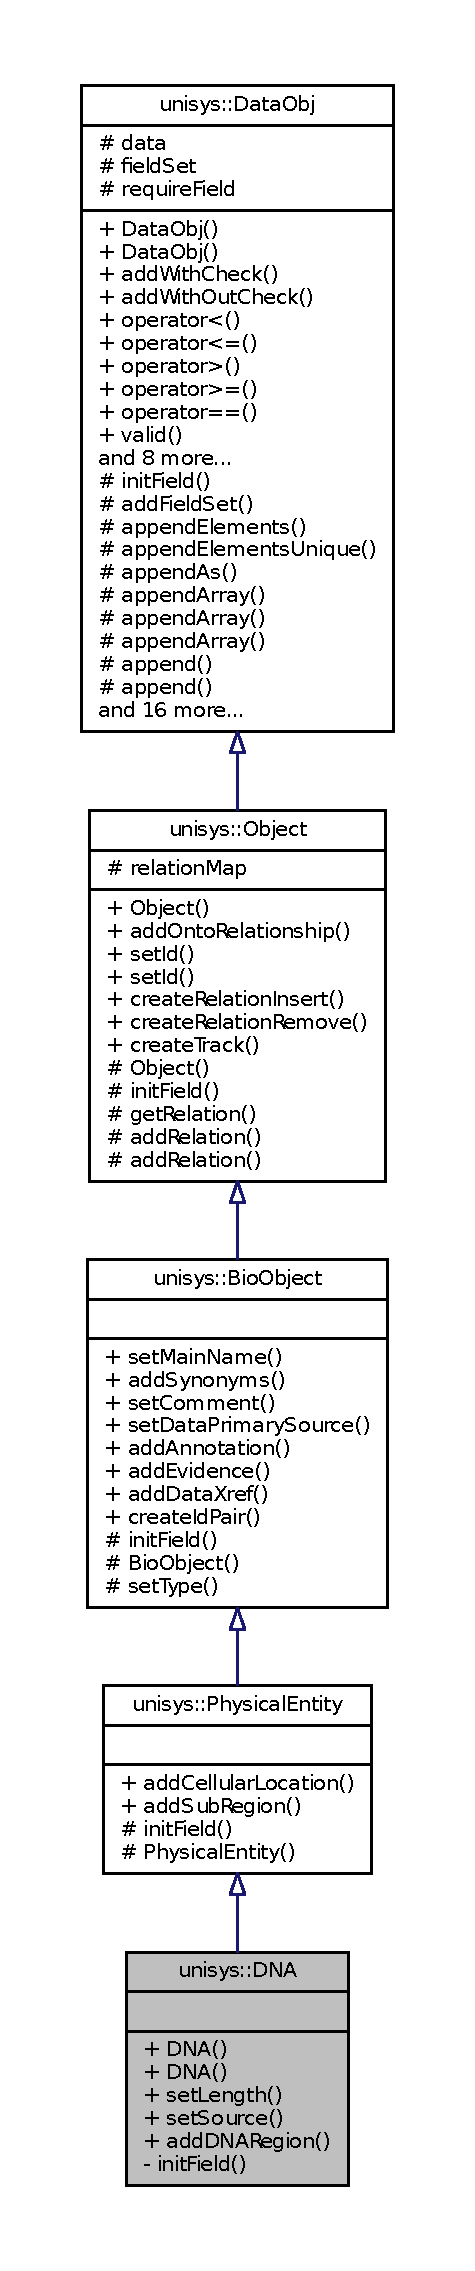
\includegraphics[height=550pt]{classunisys_1_1DNA__inherit__graph}
\end{center}
\end{figure}


Collaboration diagram for unisys\-:\-:D\-N\-A\-:
\nopagebreak
\begin{figure}[H]
\begin{center}
\leavevmode
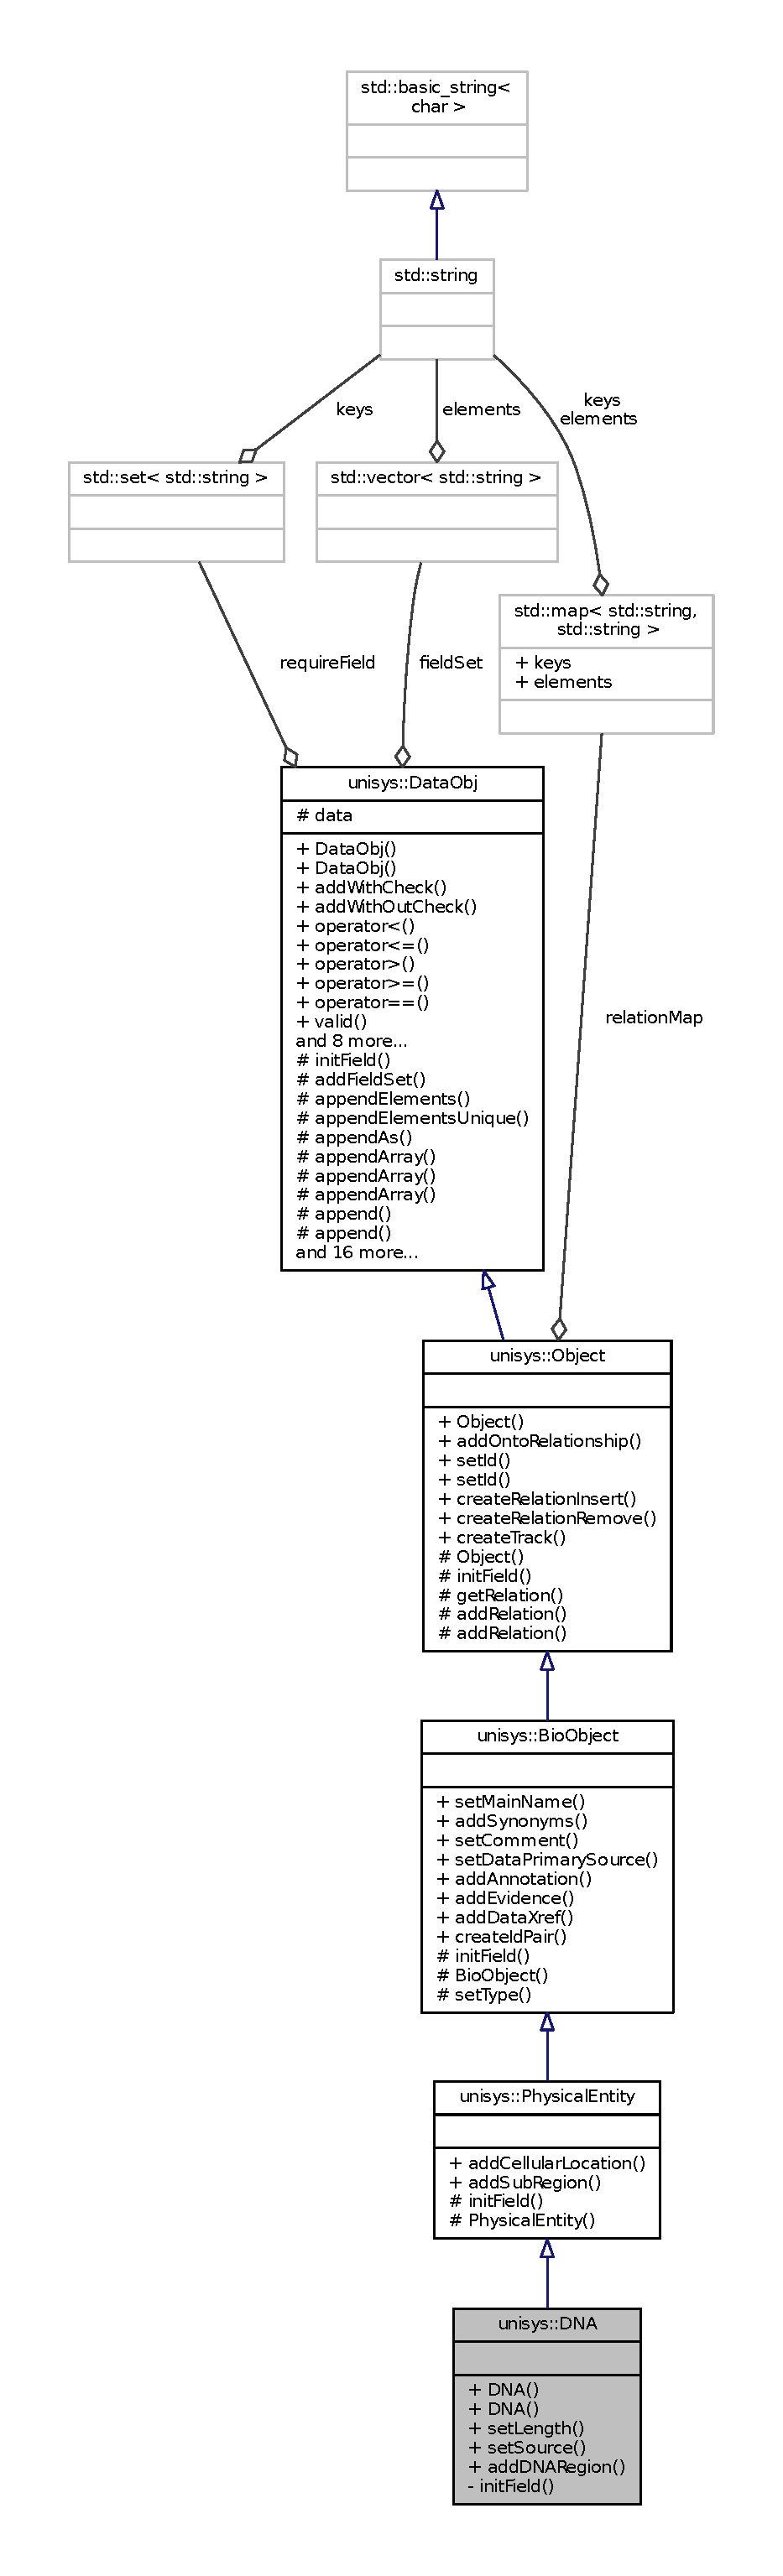
\includegraphics[height=550pt]{classunisys_1_1DNA__coll__graph}
\end{center}
\end{figure}
\subsection*{Public Member Functions}
\begin{DoxyCompactItemize}
\item 
\hyperlink{classunisys_1_1DNA_a04f18838e08019bc77fa915c862f2101}{D\-N\-A} ()
\begin{DoxyCompactList}\small\item\em Default constructor. \end{DoxyCompactList}\item 
\hyperlink{classunisys_1_1DNA_a938775f5235b21afabc2b67337e432d9}{D\-N\-A} (mongo\-::\-B\-S\-O\-N\-Obj const \&bson\-Obj)
\begin{DoxyCompactList}\small\item\em Overloaded constructor is used when retriving data in boson object from database and tranform to C++ object. \end{DoxyCompactList}\item 
void \hyperlink{classunisys_1_1DNA_aa27eef63f50cceb6da6151b3298f15e9}{set\-Length} (int length)
\item 
void \hyperlink{classunisys_1_1DNA_acf51d4eb773620fd9b622e89539e28c3}{set\-Source} (\hyperlink{classunisys_1_1BioSource}{Bio\-Source} \&source)
\item 
void \hyperlink{classunisys_1_1DNA_aa368cd88c26fd4f81e555fbbfc5f3901}{add\-D\-N\-A\-Region} (\hyperlink{classunisys_1_1PEIdRef}{P\-E\-Id\-Ref} \&dna\-Region)
\end{DoxyCompactItemize}
\subsection*{Private Member Functions}
\begin{DoxyCompactItemize}
\item 
void \hyperlink{classunisys_1_1DNA_aa33eff29fbf57aa7c626999ade40910d}{init\-Field} ()
\end{DoxyCompactItemize}
\subsection*{Additional Inherited Members}


\subsection{Detailed Description}
This class is for miriam cross reference annotation. 

\begin{DoxyVerb}        BSON structure:
        {   
            _id: <string>, #madatory
            ontologyRelationship: {<RelationshipBOSON>, <RelationshipBOSON>, ...},
            name: {<string>,<string>, ...}
            comment: <string>,
            dataPrimarySource: <XrefBOSON>,
            functionAnnotation: {<AnnotationBOSON>, <AnnotationBOSON>, ...},
            evidence: {<EvidenceBOSON>, <EvidenceBOSON>, ...},
            dataxref: {<XrefBOSON>, <XrefBOSON>, ...},
            interaction: {<DbRef>, <DbRef>, ...},
            complex: {<DbRef>, <DbRef>, ...},
            subRegion: {<SubRegionBOSON>, <SubRegionBOSON>, ...},
            length: <int>,
            source: <BioSourceBOSON>,
            dnaRegion: {<DbRef>, <DbRef>, ...}
        }\end{DoxyVerb}
 

\subsection{Constructor \& Destructor Documentation}
\hypertarget{classunisys_1_1DNA_a04f18838e08019bc77fa915c862f2101}{\index{unisys\-::\-D\-N\-A@{unisys\-::\-D\-N\-A}!D\-N\-A@{D\-N\-A}}
\index{D\-N\-A@{D\-N\-A}!unisys::DNA@{unisys\-::\-D\-N\-A}}
\subsubsection[{D\-N\-A}]{\setlength{\rightskip}{0pt plus 5cm}unisys\-::\-D\-N\-A\-::\-D\-N\-A (
\begin{DoxyParamCaption}
{}
\end{DoxyParamCaption}
)}}\label{classunisys_1_1DNA_a04f18838e08019bc77fa915c862f2101}


Default constructor. 

\hypertarget{classunisys_1_1DNA_a938775f5235b21afabc2b67337e432d9}{\index{unisys\-::\-D\-N\-A@{unisys\-::\-D\-N\-A}!D\-N\-A@{D\-N\-A}}
\index{D\-N\-A@{D\-N\-A}!unisys::DNA@{unisys\-::\-D\-N\-A}}
\subsubsection[{D\-N\-A}]{\setlength{\rightskip}{0pt plus 5cm}unisys\-::\-D\-N\-A\-::\-D\-N\-A (
\begin{DoxyParamCaption}
\item[{mongo\-::\-B\-S\-O\-N\-Obj const \&}]{bson\-Obj}
\end{DoxyParamCaption}
)}}\label{classunisys_1_1DNA_a938775f5235b21afabc2b67337e432d9}


Overloaded constructor is used when retriving data in boson object from database and tranform to C++ object. 



\subsection{Member Function Documentation}
\hypertarget{classunisys_1_1DNA_aa368cd88c26fd4f81e555fbbfc5f3901}{\index{unisys\-::\-D\-N\-A@{unisys\-::\-D\-N\-A}!add\-D\-N\-A\-Region@{add\-D\-N\-A\-Region}}
\index{add\-D\-N\-A\-Region@{add\-D\-N\-A\-Region}!unisys::DNA@{unisys\-::\-D\-N\-A}}
\subsubsection[{add\-D\-N\-A\-Region}]{\setlength{\rightskip}{0pt plus 5cm}void unisys\-::\-D\-N\-A\-::add\-D\-N\-A\-Region (
\begin{DoxyParamCaption}
\item[{{\bf P\-E\-Id\-Ref} \&}]{dna\-Region}
\end{DoxyParamCaption}
)}}\label{classunisys_1_1DNA_aa368cd88c26fd4f81e555fbbfc5f3901}
\hypertarget{classunisys_1_1DNA_aa33eff29fbf57aa7c626999ade40910d}{\index{unisys\-::\-D\-N\-A@{unisys\-::\-D\-N\-A}!init\-Field@{init\-Field}}
\index{init\-Field@{init\-Field}!unisys::DNA@{unisys\-::\-D\-N\-A}}
\subsubsection[{init\-Field}]{\setlength{\rightskip}{0pt plus 5cm}void unisys\-::\-D\-N\-A\-::init\-Field (
\begin{DoxyParamCaption}
{}
\end{DoxyParamCaption}
)\hspace{0.3cm}{\ttfamily [private]}, {\ttfamily [virtual]}}}\label{classunisys_1_1DNA_aa33eff29fbf57aa7c626999ade40910d}


Reimplemented from \hyperlink{classunisys_1_1PhysicalEntity_ad445727cb6b1c12e954819d8207104e8}{unisys\-::\-Physical\-Entity}.

\hypertarget{classunisys_1_1DNA_aa27eef63f50cceb6da6151b3298f15e9}{\index{unisys\-::\-D\-N\-A@{unisys\-::\-D\-N\-A}!set\-Length@{set\-Length}}
\index{set\-Length@{set\-Length}!unisys::DNA@{unisys\-::\-D\-N\-A}}
\subsubsection[{set\-Length}]{\setlength{\rightskip}{0pt plus 5cm}void unisys\-::\-D\-N\-A\-::set\-Length (
\begin{DoxyParamCaption}
\item[{int}]{length}
\end{DoxyParamCaption}
)}}\label{classunisys_1_1DNA_aa27eef63f50cceb6da6151b3298f15e9}
\hypertarget{classunisys_1_1DNA_acf51d4eb773620fd9b622e89539e28c3}{\index{unisys\-::\-D\-N\-A@{unisys\-::\-D\-N\-A}!set\-Source@{set\-Source}}
\index{set\-Source@{set\-Source}!unisys::DNA@{unisys\-::\-D\-N\-A}}
\subsubsection[{set\-Source}]{\setlength{\rightskip}{0pt plus 5cm}void unisys\-::\-D\-N\-A\-::set\-Source (
\begin{DoxyParamCaption}
\item[{{\bf Bio\-Source} \&}]{source}
\end{DoxyParamCaption}
)}}\label{classunisys_1_1DNA_acf51d4eb773620fd9b622e89539e28c3}


The documentation for this class was generated from the following file\-:\begin{DoxyCompactItemize}
\item 
\hyperlink{ObjClass_8h}{Obj\-Class.\-h}\end{DoxyCompactItemize}

\hypertarget{classunisys_1_1DNARegion}{\section{unisys\-:\-:D\-N\-A\-Region Class Reference}
\label{classunisys_1_1DNARegion}\index{unisys\-::\-D\-N\-A\-Region@{unisys\-::\-D\-N\-A\-Region}}
}


This class is for miriam cross reference annotation.  




{\ttfamily \#include $<$Obj\-Class.\-h$>$}



Inheritance diagram for unisys\-:\-:D\-N\-A\-Region\-:
\nopagebreak
\begin{figure}[H]
\begin{center}
\leavevmode
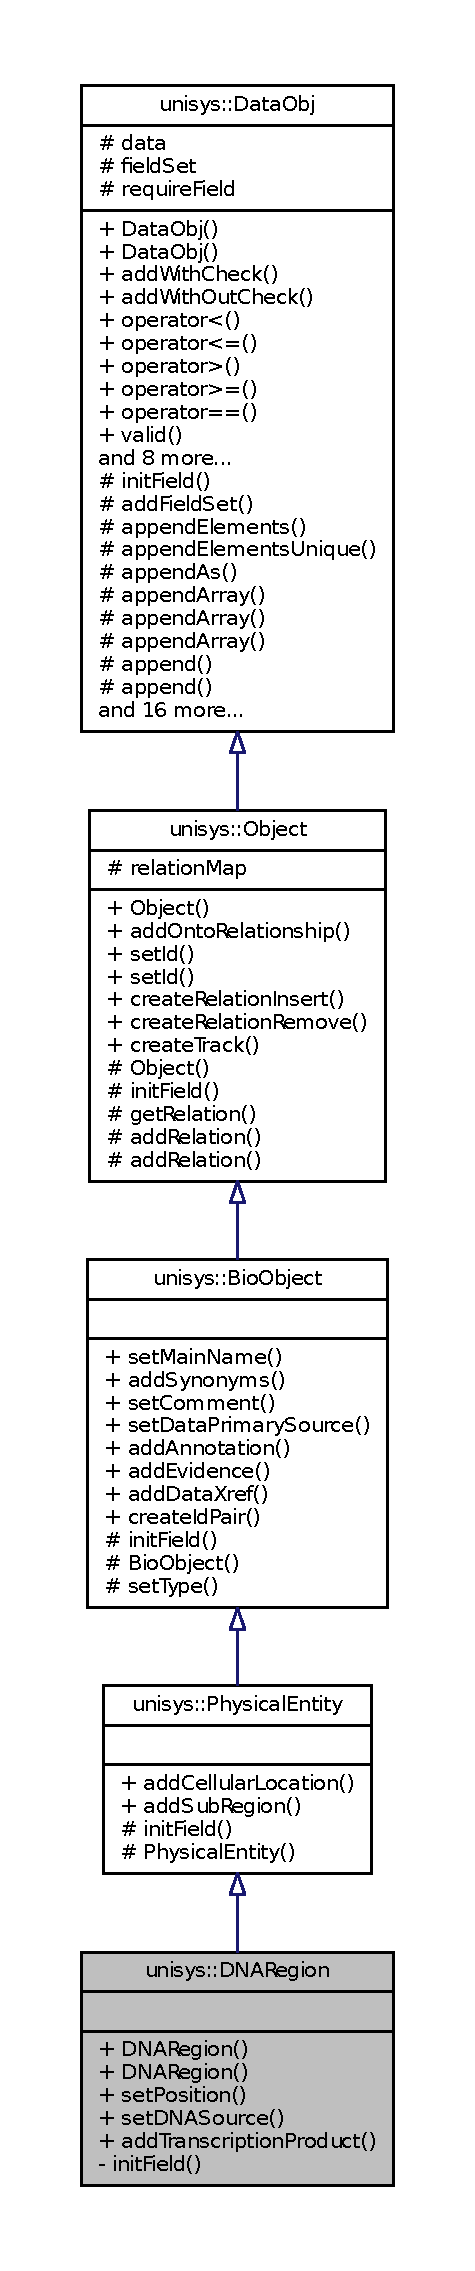
\includegraphics[height=550pt]{classunisys_1_1DNARegion__inherit__graph}
\end{center}
\end{figure}


Collaboration diagram for unisys\-:\-:D\-N\-A\-Region\-:
\nopagebreak
\begin{figure}[H]
\begin{center}
\leavevmode
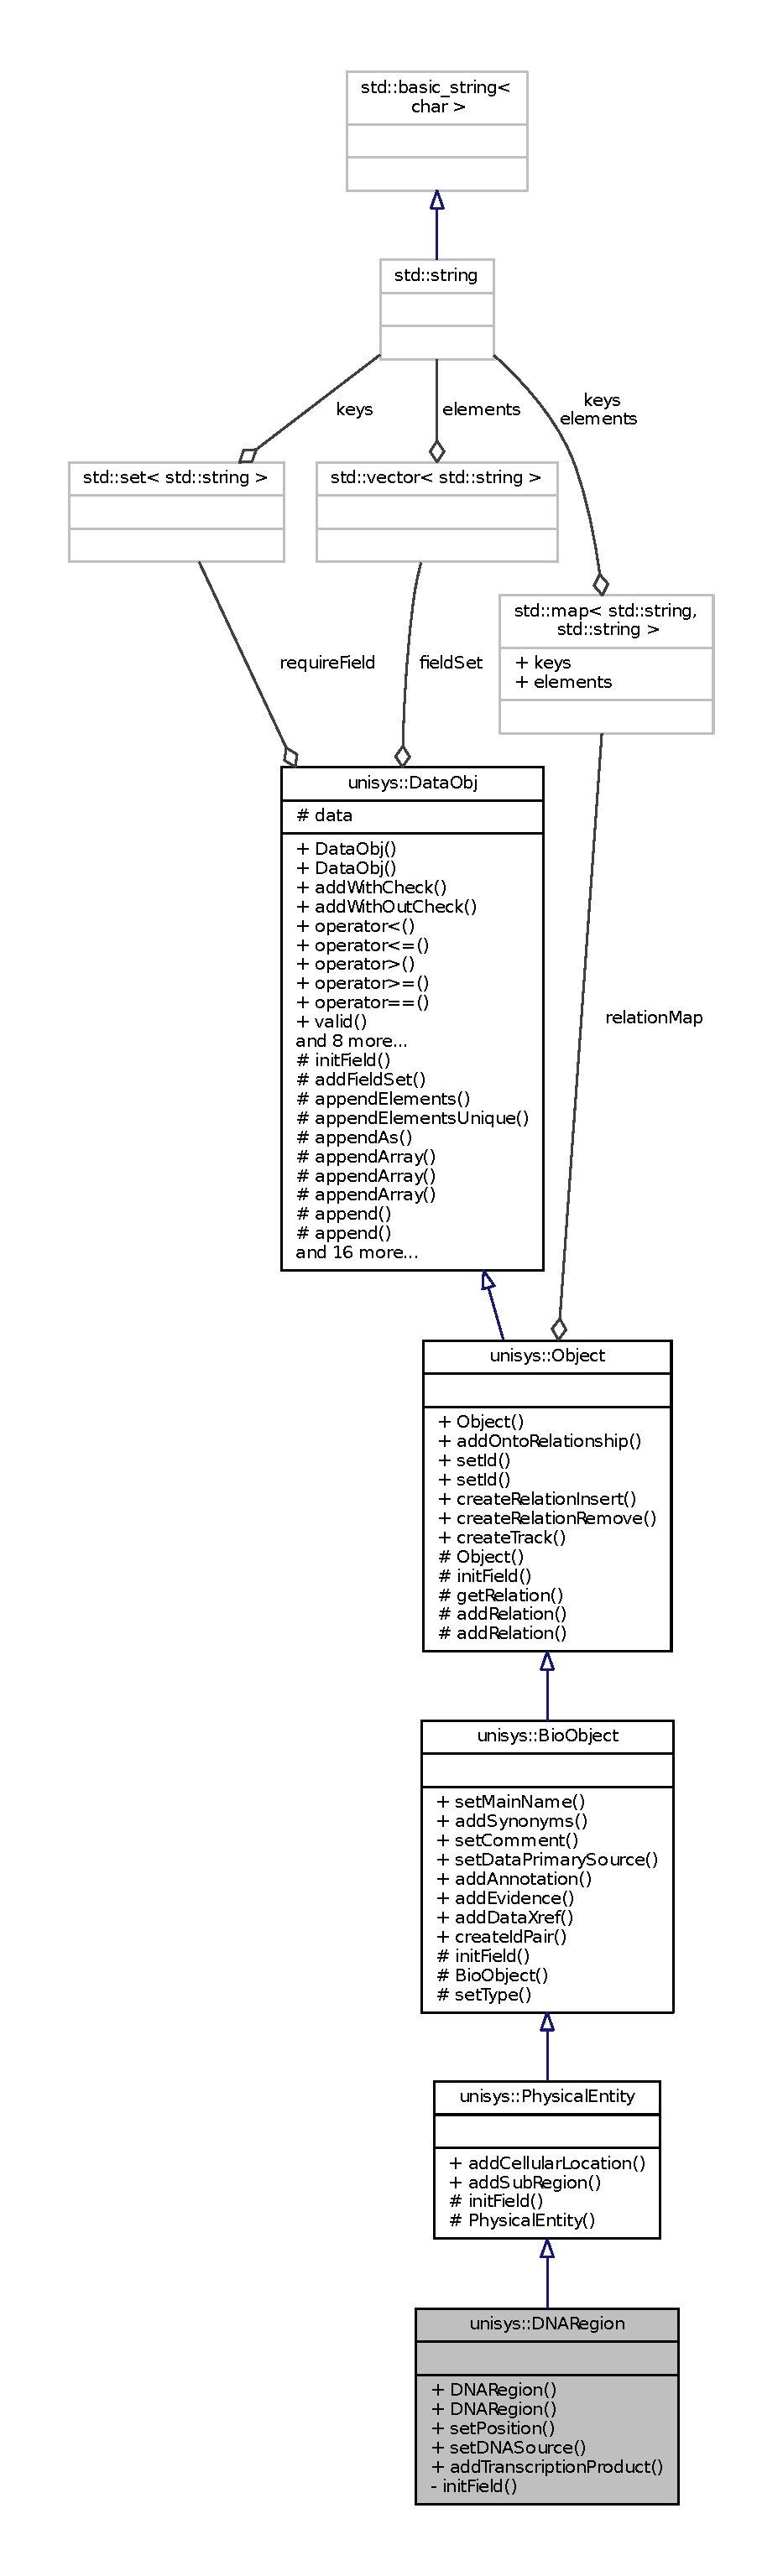
\includegraphics[height=550pt]{classunisys_1_1DNARegion__coll__graph}
\end{center}
\end{figure}
\subsection*{Public Member Functions}
\begin{DoxyCompactItemize}
\item 
\hyperlink{classunisys_1_1DNARegion_af142125cfb0ab547f47e00bd96a66c0b}{D\-N\-A\-Region} ()
\begin{DoxyCompactList}\small\item\em Default constructor. \end{DoxyCompactList}\item 
\hyperlink{classunisys_1_1DNARegion_a9fe4a81c75d6af75126e4962c0adb40a}{D\-N\-A\-Region} (mongo\-::\-B\-S\-O\-N\-Obj const \&bson\-Obj)
\begin{DoxyCompactList}\small\item\em Overloaded constructor is used when retriving data in boson object from database and tranform to C++ object. \end{DoxyCompactList}\item 
void \hyperlink{classunisys_1_1DNARegion_a50fb9c5129cbcf18d0603dc177ca7fd1}{set\-Position} (unsigned int start, unsigned int stop)
\item 
void \hyperlink{classunisys_1_1DNARegion_ac66d69ad5a779ba72bdf54e099085948}{set\-D\-N\-A\-Source} (\hyperlink{classunisys_1_1PEIdRef}{P\-E\-Id\-Ref} \&pe\-Id\-Ref)
\item 
void \hyperlink{classunisys_1_1DNARegion_a33a75b0bcde3731bfbc76770a564ed06}{add\-Transcription\-Product} (\hyperlink{classunisys_1_1PEIdRef}{P\-E\-Id\-Ref} \&trans)
\end{DoxyCompactItemize}
\subsection*{Private Member Functions}
\begin{DoxyCompactItemize}
\item 
void \hyperlink{classunisys_1_1DNARegion_a213d2340cc8f4172e3f220f1fe9883f1}{init\-Field} ()
\end{DoxyCompactItemize}
\subsection*{Additional Inherited Members}


\subsection{Detailed Description}
This class is for miriam cross reference annotation. 

\begin{DoxyVerb}        BSON structure:
        {   
            _id: <string>, #madatory
            ontologyRelationship: {<RelationshipBOSON>, <RelationshipBOSON>, ...},
            name: {<string>,<string>, ...}
            comment: <string>,
            dataPrimarySource: <XrefBOSON>,
            functionAnnotation: {<AnnotationBOSON>, <AnnotationBOSON>, ...},
            evidence: {<EvidenceBOSON>, <EvidenceBOSON>, ...},
            dataxref: {<XrefBOSON>, <XrefBOSON>, ...},
            interaction: {<DbRef>, <DbRef>, ...},
            complex: {<DbRef>, <DbRef>, ...},
            subRegion: {<SubRegionBOSON>, <SubRegionBOSON>, ...}
            position: <positionPairBSON>,
            dnaSource: <DbRef>,
            transcriptionProduct: {<DbRef>, <DbRef>, ...}
        }\end{DoxyVerb}
 

\subsection{Constructor \& Destructor Documentation}
\hypertarget{classunisys_1_1DNARegion_af142125cfb0ab547f47e00bd96a66c0b}{\index{unisys\-::\-D\-N\-A\-Region@{unisys\-::\-D\-N\-A\-Region}!D\-N\-A\-Region@{D\-N\-A\-Region}}
\index{D\-N\-A\-Region@{D\-N\-A\-Region}!unisys::DNARegion@{unisys\-::\-D\-N\-A\-Region}}
\subsubsection[{D\-N\-A\-Region}]{\setlength{\rightskip}{0pt plus 5cm}unisys\-::\-D\-N\-A\-Region\-::\-D\-N\-A\-Region (
\begin{DoxyParamCaption}
{}
\end{DoxyParamCaption}
)}}\label{classunisys_1_1DNARegion_af142125cfb0ab547f47e00bd96a66c0b}


Default constructor. 

\hypertarget{classunisys_1_1DNARegion_a9fe4a81c75d6af75126e4962c0adb40a}{\index{unisys\-::\-D\-N\-A\-Region@{unisys\-::\-D\-N\-A\-Region}!D\-N\-A\-Region@{D\-N\-A\-Region}}
\index{D\-N\-A\-Region@{D\-N\-A\-Region}!unisys::DNARegion@{unisys\-::\-D\-N\-A\-Region}}
\subsubsection[{D\-N\-A\-Region}]{\setlength{\rightskip}{0pt plus 5cm}unisys\-::\-D\-N\-A\-Region\-::\-D\-N\-A\-Region (
\begin{DoxyParamCaption}
\item[{mongo\-::\-B\-S\-O\-N\-Obj const \&}]{bson\-Obj}
\end{DoxyParamCaption}
)}}\label{classunisys_1_1DNARegion_a9fe4a81c75d6af75126e4962c0adb40a}


Overloaded constructor is used when retriving data in boson object from database and tranform to C++ object. 



\subsection{Member Function Documentation}
\hypertarget{classunisys_1_1DNARegion_a33a75b0bcde3731bfbc76770a564ed06}{\index{unisys\-::\-D\-N\-A\-Region@{unisys\-::\-D\-N\-A\-Region}!add\-Transcription\-Product@{add\-Transcription\-Product}}
\index{add\-Transcription\-Product@{add\-Transcription\-Product}!unisys::DNARegion@{unisys\-::\-D\-N\-A\-Region}}
\subsubsection[{add\-Transcription\-Product}]{\setlength{\rightskip}{0pt plus 5cm}void unisys\-::\-D\-N\-A\-Region\-::add\-Transcription\-Product (
\begin{DoxyParamCaption}
\item[{{\bf P\-E\-Id\-Ref} \&}]{trans}
\end{DoxyParamCaption}
)}}\label{classunisys_1_1DNARegion_a33a75b0bcde3731bfbc76770a564ed06}
\hypertarget{classunisys_1_1DNARegion_a213d2340cc8f4172e3f220f1fe9883f1}{\index{unisys\-::\-D\-N\-A\-Region@{unisys\-::\-D\-N\-A\-Region}!init\-Field@{init\-Field}}
\index{init\-Field@{init\-Field}!unisys::DNARegion@{unisys\-::\-D\-N\-A\-Region}}
\subsubsection[{init\-Field}]{\setlength{\rightskip}{0pt plus 5cm}void unisys\-::\-D\-N\-A\-Region\-::init\-Field (
\begin{DoxyParamCaption}
{}
\end{DoxyParamCaption}
)\hspace{0.3cm}{\ttfamily [private]}, {\ttfamily [virtual]}}}\label{classunisys_1_1DNARegion_a213d2340cc8f4172e3f220f1fe9883f1}


Reimplemented from \hyperlink{classunisys_1_1PhysicalEntity_ad445727cb6b1c12e954819d8207104e8}{unisys\-::\-Physical\-Entity}.

\hypertarget{classunisys_1_1DNARegion_ac66d69ad5a779ba72bdf54e099085948}{\index{unisys\-::\-D\-N\-A\-Region@{unisys\-::\-D\-N\-A\-Region}!set\-D\-N\-A\-Source@{set\-D\-N\-A\-Source}}
\index{set\-D\-N\-A\-Source@{set\-D\-N\-A\-Source}!unisys::DNARegion@{unisys\-::\-D\-N\-A\-Region}}
\subsubsection[{set\-D\-N\-A\-Source}]{\setlength{\rightskip}{0pt plus 5cm}void unisys\-::\-D\-N\-A\-Region\-::set\-D\-N\-A\-Source (
\begin{DoxyParamCaption}
\item[{{\bf P\-E\-Id\-Ref} \&}]{pe\-Id\-Ref}
\end{DoxyParamCaption}
)}}\label{classunisys_1_1DNARegion_ac66d69ad5a779ba72bdf54e099085948}
\hypertarget{classunisys_1_1DNARegion_a50fb9c5129cbcf18d0603dc177ca7fd1}{\index{unisys\-::\-D\-N\-A\-Region@{unisys\-::\-D\-N\-A\-Region}!set\-Position@{set\-Position}}
\index{set\-Position@{set\-Position}!unisys::DNARegion@{unisys\-::\-D\-N\-A\-Region}}
\subsubsection[{set\-Position}]{\setlength{\rightskip}{0pt plus 5cm}void unisys\-::\-D\-N\-A\-Region\-::set\-Position (
\begin{DoxyParamCaption}
\item[{unsigned int}]{start, }
\item[{unsigned int}]{stop}
\end{DoxyParamCaption}
)}}\label{classunisys_1_1DNARegion_a50fb9c5129cbcf18d0603dc177ca7fd1}


The documentation for this class was generated from the following file\-:\begin{DoxyCompactItemize}
\item 
\hyperlink{ObjClass_8h}{Obj\-Class.\-h}\end{DoxyCompactItemize}

\hypertarget{classunisys_1_1Evidence}{\section{unisys\-:\-:Evidence Class Reference}
\label{classunisys_1_1Evidence}\index{unisys\-::\-Evidence@{unisys\-::\-Evidence}}
}


The C++ representative class for evidence data class.  




{\ttfamily \#include $<$Lit\-Class.\-h$>$}



Inheritance diagram for unisys\-:\-:Evidence\-:
\nopagebreak
\begin{figure}[H]
\begin{center}
\leavevmode
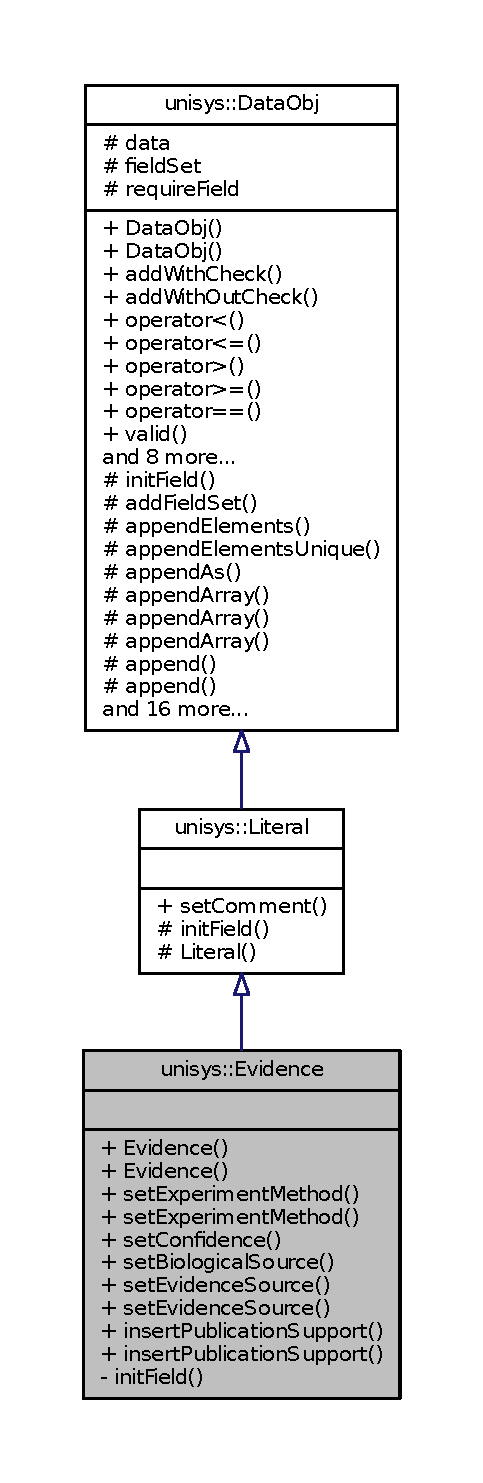
\includegraphics[height=550pt]{classunisys_1_1Evidence__inherit__graph}
\end{center}
\end{figure}


Collaboration diagram for unisys\-:\-:Evidence\-:
\nopagebreak
\begin{figure}[H]
\begin{center}
\leavevmode
\includegraphics[height=550pt]{classunisys_1_1Evidence__coll__graph}
\end{center}
\end{figure}
\subsection*{Public Member Functions}
\begin{DoxyCompactItemize}
\item 
\hyperlink{classunisys_1_1Evidence_ae8c055dcc1043da7a655487931f67864}{Evidence} ()
\begin{DoxyCompactList}\small\item\em Default constructor. \end{DoxyCompactList}\item 
\hyperlink{classunisys_1_1Evidence_ab349472863abf438f40c5f2f089281ac}{Evidence} (mongo\-::\-B\-S\-O\-N\-Obj const \&bson\-Obj)
\begin{DoxyCompactList}\small\item\em Overloaded constructor is used when retriving data in boson object from database and tranform to C++ object. \end{DoxyCompactList}\item 
void \hyperlink{classunisys_1_1Evidence_a6b74b64b25249e38e9b2524c8882adca}{set\-Experiment\-Method} (\hyperlink{classunisys_1_1OntoIdRef}{Onto\-Id\-Ref} \&onto\-Id\-Ref)
\item 
void \hyperlink{classunisys_1_1Evidence_a10bdc5b89865dea993dde0782270c836}{set\-Experiment\-Method} (std\-::string const \&onto\-Id)
\item 
void \hyperlink{classunisys_1_1Evidence_a9bc4f40a58aae2b0fafc73ed0d647d5a}{set\-Confidence} (\hyperlink{classunisys_1_1Score}{Score} \&score)
\item 
void \hyperlink{classunisys_1_1Evidence_a7cbfcbc96a2364d268012c09df1e6eca}{set\-Biological\-Source} (\hyperlink{classunisys_1_1BioSource}{Bio\-Source} \&biological\-Source)
\item 
void \hyperlink{classunisys_1_1Evidence_a3d9c295abcdaf773621427536d742b8b}{set\-Evidence\-Source} (\hyperlink{classunisys_1_1Xref}{Xref} \&evidence\-Source)
\item 
void \hyperlink{classunisys_1_1Evidence_a5bf3367415dbe2e37dfcff827101c65d}{set\-Evidence\-Source} (std\-::string const \&evidence\-Source\-Id, std\-::string const \&detail=\char`\"{}\char`\"{})
\item 
void \hyperlink{classunisys_1_1Evidence_ac3ecf7240bc24d235f2ee1226e9be83e}{insert\-Publication\-Support} (\hyperlink{classunisys_1_1Xref}{Xref} \&publication\-Support)
\item 
void \hyperlink{classunisys_1_1Evidence_a16f5abbb62d6231681b74244d8060cb8}{insert\-Publication\-Support} (std\-::string const \&publication\-Support\-Id, std\-::string const \&detail=\char`\"{}\char`\"{})
\end{DoxyCompactItemize}
\subsection*{Private Member Functions}
\begin{DoxyCompactItemize}
\item 
void \hyperlink{classunisys_1_1Evidence_a8ce7e3da30295b98aa095031ef8491bc}{init\-Field} ()
\begin{DoxyCompactList}\small\item\em function for init field in the object \end{DoxyCompactList}\end{DoxyCompactItemize}
\subsection*{Additional Inherited Members}


\subsection{Detailed Description}
The C++ representative class for evidence data class. 

\begin{DoxyVerb}        BSON structure:
        {   
            comment: <string>,
            experimentMethod: {$ref: <collname>, $id: <idvalue>}, #format by idref class
            score: <ScoreBSONStructure>,
            biologicalSource: <BioSourceBSONStructure>,
            evidenceSource: <XRefBSONStructure>,
            publicationSupport: {<XRefBSONStructure>, <XRefBSONStructure>, ...}
        }\end{DoxyVerb}
 

\subsection{Constructor \& Destructor Documentation}
\hypertarget{classunisys_1_1Evidence_ae8c055dcc1043da7a655487931f67864}{\index{unisys\-::\-Evidence@{unisys\-::\-Evidence}!Evidence@{Evidence}}
\index{Evidence@{Evidence}!unisys::Evidence@{unisys\-::\-Evidence}}
\subsubsection[{Evidence}]{\setlength{\rightskip}{0pt plus 5cm}unisys\-::\-Evidence\-::\-Evidence (
\begin{DoxyParamCaption}
{}
\end{DoxyParamCaption}
)}}\label{classunisys_1_1Evidence_ae8c055dcc1043da7a655487931f67864}


Default constructor. 

\hypertarget{classunisys_1_1Evidence_ab349472863abf438f40c5f2f089281ac}{\index{unisys\-::\-Evidence@{unisys\-::\-Evidence}!Evidence@{Evidence}}
\index{Evidence@{Evidence}!unisys::Evidence@{unisys\-::\-Evidence}}
\subsubsection[{Evidence}]{\setlength{\rightskip}{0pt plus 5cm}unisys\-::\-Evidence\-::\-Evidence (
\begin{DoxyParamCaption}
\item[{mongo\-::\-B\-S\-O\-N\-Obj const \&}]{bson\-Obj}
\end{DoxyParamCaption}
)}}\label{classunisys_1_1Evidence_ab349472863abf438f40c5f2f089281ac}


Overloaded constructor is used when retriving data in boson object from database and tranform to C++ object. 



\subsection{Member Function Documentation}
\hypertarget{classunisys_1_1Evidence_a8ce7e3da30295b98aa095031ef8491bc}{\index{unisys\-::\-Evidence@{unisys\-::\-Evidence}!init\-Field@{init\-Field}}
\index{init\-Field@{init\-Field}!unisys::Evidence@{unisys\-::\-Evidence}}
\subsubsection[{init\-Field}]{\setlength{\rightskip}{0pt plus 5cm}void unisys\-::\-Evidence\-::init\-Field (
\begin{DoxyParamCaption}
{}
\end{DoxyParamCaption}
)\hspace{0.3cm}{\ttfamily [private]}, {\ttfamily [virtual]}}}\label{classunisys_1_1Evidence_a8ce7e3da30295b98aa095031ef8491bc}


function for init field in the object 



Reimplemented from \hyperlink{classunisys_1_1Literal_a769b8f41e99619d8635f83d18a02bc1f}{unisys\-::\-Literal}.

\hypertarget{classunisys_1_1Evidence_ac3ecf7240bc24d235f2ee1226e9be83e}{\index{unisys\-::\-Evidence@{unisys\-::\-Evidence}!insert\-Publication\-Support@{insert\-Publication\-Support}}
\index{insert\-Publication\-Support@{insert\-Publication\-Support}!unisys::Evidence@{unisys\-::\-Evidence}}
\subsubsection[{insert\-Publication\-Support}]{\setlength{\rightskip}{0pt plus 5cm}void unisys\-::\-Evidence\-::insert\-Publication\-Support (
\begin{DoxyParamCaption}
\item[{{\bf Xref} \&}]{publication\-Support}
\end{DoxyParamCaption}
)}}\label{classunisys_1_1Evidence_ac3ecf7240bc24d235f2ee1226e9be83e}
\hypertarget{classunisys_1_1Evidence_a16f5abbb62d6231681b74244d8060cb8}{\index{unisys\-::\-Evidence@{unisys\-::\-Evidence}!insert\-Publication\-Support@{insert\-Publication\-Support}}
\index{insert\-Publication\-Support@{insert\-Publication\-Support}!unisys::Evidence@{unisys\-::\-Evidence}}
\subsubsection[{insert\-Publication\-Support}]{\setlength{\rightskip}{0pt plus 5cm}void unisys\-::\-Evidence\-::insert\-Publication\-Support (
\begin{DoxyParamCaption}
\item[{std\-::string const \&}]{publication\-Support\-Id, }
\item[{std\-::string const \&}]{detail = {\ttfamily \char`\"{}\char`\"{}}}
\end{DoxyParamCaption}
)}}\label{classunisys_1_1Evidence_a16f5abbb62d6231681b74244d8060cb8}
\hypertarget{classunisys_1_1Evidence_a7cbfcbc96a2364d268012c09df1e6eca}{\index{unisys\-::\-Evidence@{unisys\-::\-Evidence}!set\-Biological\-Source@{set\-Biological\-Source}}
\index{set\-Biological\-Source@{set\-Biological\-Source}!unisys::Evidence@{unisys\-::\-Evidence}}
\subsubsection[{set\-Biological\-Source}]{\setlength{\rightskip}{0pt plus 5cm}void unisys\-::\-Evidence\-::set\-Biological\-Source (
\begin{DoxyParamCaption}
\item[{{\bf Bio\-Source} \&}]{biological\-Source}
\end{DoxyParamCaption}
)}}\label{classunisys_1_1Evidence_a7cbfcbc96a2364d268012c09df1e6eca}
\hypertarget{classunisys_1_1Evidence_a9bc4f40a58aae2b0fafc73ed0d647d5a}{\index{unisys\-::\-Evidence@{unisys\-::\-Evidence}!set\-Confidence@{set\-Confidence}}
\index{set\-Confidence@{set\-Confidence}!unisys::Evidence@{unisys\-::\-Evidence}}
\subsubsection[{set\-Confidence}]{\setlength{\rightskip}{0pt plus 5cm}void unisys\-::\-Evidence\-::set\-Confidence (
\begin{DoxyParamCaption}
\item[{{\bf Score} \&}]{score}
\end{DoxyParamCaption}
)}}\label{classunisys_1_1Evidence_a9bc4f40a58aae2b0fafc73ed0d647d5a}
\hypertarget{classunisys_1_1Evidence_a3d9c295abcdaf773621427536d742b8b}{\index{unisys\-::\-Evidence@{unisys\-::\-Evidence}!set\-Evidence\-Source@{set\-Evidence\-Source}}
\index{set\-Evidence\-Source@{set\-Evidence\-Source}!unisys::Evidence@{unisys\-::\-Evidence}}
\subsubsection[{set\-Evidence\-Source}]{\setlength{\rightskip}{0pt plus 5cm}void unisys\-::\-Evidence\-::set\-Evidence\-Source (
\begin{DoxyParamCaption}
\item[{{\bf Xref} \&}]{evidence\-Source}
\end{DoxyParamCaption}
)}}\label{classunisys_1_1Evidence_a3d9c295abcdaf773621427536d742b8b}
\hypertarget{classunisys_1_1Evidence_a5bf3367415dbe2e37dfcff827101c65d}{\index{unisys\-::\-Evidence@{unisys\-::\-Evidence}!set\-Evidence\-Source@{set\-Evidence\-Source}}
\index{set\-Evidence\-Source@{set\-Evidence\-Source}!unisys::Evidence@{unisys\-::\-Evidence}}
\subsubsection[{set\-Evidence\-Source}]{\setlength{\rightskip}{0pt plus 5cm}void unisys\-::\-Evidence\-::set\-Evidence\-Source (
\begin{DoxyParamCaption}
\item[{std\-::string const \&}]{evidence\-Source\-Id, }
\item[{std\-::string const \&}]{detail = {\ttfamily \char`\"{}\char`\"{}}}
\end{DoxyParamCaption}
)}}\label{classunisys_1_1Evidence_a5bf3367415dbe2e37dfcff827101c65d}
\hypertarget{classunisys_1_1Evidence_a6b74b64b25249e38e9b2524c8882adca}{\index{unisys\-::\-Evidence@{unisys\-::\-Evidence}!set\-Experiment\-Method@{set\-Experiment\-Method}}
\index{set\-Experiment\-Method@{set\-Experiment\-Method}!unisys::Evidence@{unisys\-::\-Evidence}}
\subsubsection[{set\-Experiment\-Method}]{\setlength{\rightskip}{0pt plus 5cm}void unisys\-::\-Evidence\-::set\-Experiment\-Method (
\begin{DoxyParamCaption}
\item[{{\bf Onto\-Id\-Ref} \&}]{onto\-Id\-Ref}
\end{DoxyParamCaption}
)}}\label{classunisys_1_1Evidence_a6b74b64b25249e38e9b2524c8882adca}
\hypertarget{classunisys_1_1Evidence_a10bdc5b89865dea993dde0782270c836}{\index{unisys\-::\-Evidence@{unisys\-::\-Evidence}!set\-Experiment\-Method@{set\-Experiment\-Method}}
\index{set\-Experiment\-Method@{set\-Experiment\-Method}!unisys::Evidence@{unisys\-::\-Evidence}}
\subsubsection[{set\-Experiment\-Method}]{\setlength{\rightskip}{0pt plus 5cm}void unisys\-::\-Evidence\-::set\-Experiment\-Method (
\begin{DoxyParamCaption}
\item[{std\-::string const \&}]{onto\-Id}
\end{DoxyParamCaption}
)}}\label{classunisys_1_1Evidence_a10bdc5b89865dea993dde0782270c836}


The documentation for this class was generated from the following file\-:\begin{DoxyCompactItemize}
\item 
\hyperlink{LitClass_8h}{Lit\-Class.\-h}\end{DoxyCompactItemize}

\hypertarget{classunisys_1_1GeneticInteraction}{\section{unisys\-:\-:Genetic\-Interaction Class Reference}
\label{classunisys_1_1GeneticInteraction}\index{unisys\-::\-Genetic\-Interaction@{unisys\-::\-Genetic\-Interaction}}
}


This class is for miriam cross reference annotation.  




{\ttfamily \#include $<$Obj\-Class.\-h$>$}



Inheritance diagram for unisys\-:\-:Genetic\-Interaction\-:
\nopagebreak
\begin{figure}[H]
\begin{center}
\leavevmode
\includegraphics[height=550pt]{classunisys_1_1GeneticInteraction__inherit__graph}
\end{center}
\end{figure}


Collaboration diagram for unisys\-:\-:Genetic\-Interaction\-:
\nopagebreak
\begin{figure}[H]
\begin{center}
\leavevmode
\includegraphics[height=550pt]{classunisys_1_1GeneticInteraction__coll__graph}
\end{center}
\end{figure}
\subsection*{Public Member Functions}
\begin{DoxyCompactItemize}
\item 
\hyperlink{classunisys_1_1GeneticInteraction_a53ef22c5219fa6eff75d40a464356d8e}{Genetic\-Interaction} ()
\begin{DoxyCompactList}\small\item\em Default constructor. \end{DoxyCompactList}\item 
\hyperlink{classunisys_1_1GeneticInteraction_a8a085b9625e51fce04c13477af04314f}{Genetic\-Interaction} (mongo\-::\-B\-S\-O\-N\-Obj const \&bson\-Obj)
\begin{DoxyCompactList}\small\item\em Overloaded constructor is used when retriving data in boson object from database and tranform to C++ object. \end{DoxyCompactList}\item 
void \hyperlink{classunisys_1_1GeneticInteraction_a086ef8611b4006eb33fd111c2cd109aa}{set\-Interaction\-Type} (\hyperlink{classunisys_1_1OntoIdRef}{Onto\-Id\-Ref} \&onto\-Id\-Ref)
\item 
void \hyperlink{classunisys_1_1GeneticInteraction_ae65dcf635fa1ae1a5590f0c7e718ae30}{set\-Phenotype} (\hyperlink{classunisys_1_1OntoIdRef}{Onto\-Id\-Ref} \&onto\-Id\-Ref)
\end{DoxyCompactItemize}
\subsection*{Private Member Functions}
\begin{DoxyCompactItemize}
\item 
void \hyperlink{classunisys_1_1GeneticInteraction_a946b8270db467290f49a050bd29f55d2}{init\-Field} ()
\end{DoxyCompactItemize}
\subsection*{Additional Inherited Members}


\subsection{Detailed Description}
This class is for miriam cross reference annotation. 

\begin{DoxyVerb}        BSON structure:
        {   
            _id: <string>, #madatory
            type: <string>,
            ontologyRelationship: {<RelationshipBOSON>, <RelationshipBOSON>, ...},
            name: {<string>,<string>, ...}
            comment: <string>,
            dataPrimarySource: <XrefBOSON>,
            functionAnnotation: {<AnnotationBOSON>, <AnnotationBOSON>, ...},
            evidence: {<EvidenceBOSON>, <EvidenceBOSON>, ...},
            dataxref: {<XrefBOSON>, <XrefBOSON>, ...},
            participant: {<StoichiometryBOSON>, <StoichiometryBOSON>, ...},
            interactionKey: <string>,
            interactionType: <DbRef>,
            phynotype: <DbRef>
        }\end{DoxyVerb}
 

\subsection{Constructor \& Destructor Documentation}
\hypertarget{classunisys_1_1GeneticInteraction_a53ef22c5219fa6eff75d40a464356d8e}{\index{unisys\-::\-Genetic\-Interaction@{unisys\-::\-Genetic\-Interaction}!Genetic\-Interaction@{Genetic\-Interaction}}
\index{Genetic\-Interaction@{Genetic\-Interaction}!unisys::GeneticInteraction@{unisys\-::\-Genetic\-Interaction}}
\subsubsection[{Genetic\-Interaction}]{\setlength{\rightskip}{0pt plus 5cm}unisys\-::\-Genetic\-Interaction\-::\-Genetic\-Interaction (
\begin{DoxyParamCaption}
{}
\end{DoxyParamCaption}
)}}\label{classunisys_1_1GeneticInteraction_a53ef22c5219fa6eff75d40a464356d8e}


Default constructor. 

\hypertarget{classunisys_1_1GeneticInteraction_a8a085b9625e51fce04c13477af04314f}{\index{unisys\-::\-Genetic\-Interaction@{unisys\-::\-Genetic\-Interaction}!Genetic\-Interaction@{Genetic\-Interaction}}
\index{Genetic\-Interaction@{Genetic\-Interaction}!unisys::GeneticInteraction@{unisys\-::\-Genetic\-Interaction}}
\subsubsection[{Genetic\-Interaction}]{\setlength{\rightskip}{0pt plus 5cm}unisys\-::\-Genetic\-Interaction\-::\-Genetic\-Interaction (
\begin{DoxyParamCaption}
\item[{mongo\-::\-B\-S\-O\-N\-Obj const \&}]{bson\-Obj}
\end{DoxyParamCaption}
)}}\label{classunisys_1_1GeneticInteraction_a8a085b9625e51fce04c13477af04314f}


Overloaded constructor is used when retriving data in boson object from database and tranform to C++ object. 



\subsection{Member Function Documentation}
\hypertarget{classunisys_1_1GeneticInteraction_a946b8270db467290f49a050bd29f55d2}{\index{unisys\-::\-Genetic\-Interaction@{unisys\-::\-Genetic\-Interaction}!init\-Field@{init\-Field}}
\index{init\-Field@{init\-Field}!unisys::GeneticInteraction@{unisys\-::\-Genetic\-Interaction}}
\subsubsection[{init\-Field}]{\setlength{\rightskip}{0pt plus 5cm}void unisys\-::\-Genetic\-Interaction\-::init\-Field (
\begin{DoxyParamCaption}
{}
\end{DoxyParamCaption}
)\hspace{0.3cm}{\ttfamily [private]}, {\ttfamily [virtual]}}}\label{classunisys_1_1GeneticInteraction_a946b8270db467290f49a050bd29f55d2}


Reimplemented from \hyperlink{classunisys_1_1Interaction_a84c6c3e09f83ec8dd8dec7485f97e02b}{unisys\-::\-Interaction}.

\hypertarget{classunisys_1_1GeneticInteraction_a086ef8611b4006eb33fd111c2cd109aa}{\index{unisys\-::\-Genetic\-Interaction@{unisys\-::\-Genetic\-Interaction}!set\-Interaction\-Type@{set\-Interaction\-Type}}
\index{set\-Interaction\-Type@{set\-Interaction\-Type}!unisys::GeneticInteraction@{unisys\-::\-Genetic\-Interaction}}
\subsubsection[{set\-Interaction\-Type}]{\setlength{\rightskip}{0pt plus 5cm}void unisys\-::\-Genetic\-Interaction\-::set\-Interaction\-Type (
\begin{DoxyParamCaption}
\item[{{\bf Onto\-Id\-Ref} \&}]{onto\-Id\-Ref}
\end{DoxyParamCaption}
)}}\label{classunisys_1_1GeneticInteraction_a086ef8611b4006eb33fd111c2cd109aa}
\hypertarget{classunisys_1_1GeneticInteraction_ae65dcf635fa1ae1a5590f0c7e718ae30}{\index{unisys\-::\-Genetic\-Interaction@{unisys\-::\-Genetic\-Interaction}!set\-Phenotype@{set\-Phenotype}}
\index{set\-Phenotype@{set\-Phenotype}!unisys::GeneticInteraction@{unisys\-::\-Genetic\-Interaction}}
\subsubsection[{set\-Phenotype}]{\setlength{\rightskip}{0pt plus 5cm}void unisys\-::\-Genetic\-Interaction\-::set\-Phenotype (
\begin{DoxyParamCaption}
\item[{{\bf Onto\-Id\-Ref} \&}]{onto\-Id\-Ref}
\end{DoxyParamCaption}
)}}\label{classunisys_1_1GeneticInteraction_ae65dcf635fa1ae1a5590f0c7e718ae30}


The documentation for this class was generated from the following file\-:\begin{DoxyCompactItemize}
\item 
\hyperlink{ObjClass_8h}{Obj\-Class.\-h}\end{DoxyCompactItemize}

\hypertarget{classunisys_1_1IdRef}{\section{unisys\-:\-:Id\-Ref Class Reference}
\label{classunisys_1_1IdRef}\index{unisys\-::\-Id\-Ref@{unisys\-::\-Id\-Ref}}
}


Identifier reference class.  




{\ttfamily \#include $<$D\-B\-Class.\-h$>$}



Inheritance diagram for unisys\-:\-:Id\-Ref\-:
\nopagebreak
\begin{figure}[H]
\begin{center}
\leavevmode
\includegraphics[height=550pt]{classunisys_1_1IdRef__inherit__graph}
\end{center}
\end{figure}


Collaboration diagram for unisys\-:\-:Id\-Ref\-:
\nopagebreak
\begin{figure}[H]
\begin{center}
\leavevmode
\includegraphics[height=550pt]{classunisys_1_1IdRef__coll__graph}
\end{center}
\end{figure}
\subsection*{Public Member Functions}
\begin{DoxyCompactItemize}
\item 
\hyperlink{classunisys_1_1IdRef_ac1f80a3c9603e25bf73ea649b571c628}{Id\-Ref} ()
\begin{DoxyCompactList}\small\item\em Default constructor. \end{DoxyCompactList}\item 
\hyperlink{classunisys_1_1IdRef_a02027d11b26a6e4131525c346186976d}{Id\-Ref} (mongo\-::\-B\-S\-O\-N\-Obj const \&bson\-Obj)
\begin{DoxyCompactList}\small\item\em Overloaded constructor get a B\-S\-O\-N\-Obj as parameters. \end{DoxyCompactList}\item 
\hyperlink{classunisys_1_1IdRef_afdfaf736d758f9ee321557e63a2257de}{Id\-Ref} (std\-::string const \&D\-B\-Id, std\-::string const \&collection\-N\-S)
\begin{DoxyCompactList}\small\item\em Overloaded constructor get a id string and collection\-N\-S as parameters. \end{DoxyCompactList}\item 
void \hyperlink{classunisys_1_1IdRef_a797643add7a57839526d8561156631fe}{init\-Member} (std\-::string const \&D\-B\-Id, std\-::string const \&collection\-N\-S)
\item 
std\-::string \hyperlink{classunisys_1_1IdRef_a9e002479bf85ca26d965018108036151}{get\-Id} () const 
\begin{DoxyCompactList}\small\item\em Return Id string. \end{DoxyCompactList}\item 
std\-::string \hyperlink{classunisys_1_1IdRef_aa4430b934e5305c1bdeae7bd15adeb70}{get\-N\-S} () const 
\item 
bool \hyperlink{classunisys_1_1IdRef_a4ab596023020171bceeb2aed8bd529ce}{is\-Valid} () const 
\begin{DoxyCompactList}\small\item\em Check validity of class. \end{DoxyCompactList}\end{DoxyCompactItemize}
\subsection*{Protected Member Functions}
\begin{DoxyCompactItemize}
\item 
void \hyperlink{classunisys_1_1IdRef_a2f8143648ba349f8a910ee64b10c0829}{init\-Field} ()
\begin{DoxyCompactList}\small\item\em set the field names \end{DoxyCompactList}\end{DoxyCompactItemize}
\subsection*{Additional Inherited Members}


\subsection{Detailed Description}
Identifier reference class. 

This class is used for storing database reference (D\-B\-Ref) under Mongo\-Db D\-B\-Ref format, which is \{\char`\"{}\$ref\char`\"{}\-: \char`\"{}collection\-N\-S\char`\"{}, \char`\"{}\$id\char`\"{}\-: \char`\"{}id\char`\"{}\}, but it support only reference between objects in the same database. This class provides the member functions to manage, converse to another class and to dereference the data from specific database handler.

B\-S\-O\-N structure\-: \{ \$ref\-: $<$collname$>$, \$id\-: $<$idvalue$>$, \} 

\subsection{Constructor \& Destructor Documentation}
\hypertarget{classunisys_1_1IdRef_ac1f80a3c9603e25bf73ea649b571c628}{\index{unisys\-::\-Id\-Ref@{unisys\-::\-Id\-Ref}!Id\-Ref@{Id\-Ref}}
\index{Id\-Ref@{Id\-Ref}!unisys::IdRef@{unisys\-::\-Id\-Ref}}
\subsubsection[{Id\-Ref}]{\setlength{\rightskip}{0pt plus 5cm}unisys\-::\-Id\-Ref\-::\-Id\-Ref (
\begin{DoxyParamCaption}
{}
\end{DoxyParamCaption}
)}}\label{classunisys_1_1IdRef_ac1f80a3c9603e25bf73ea649b571c628}


Default constructor. 

\hypertarget{classunisys_1_1IdRef_a02027d11b26a6e4131525c346186976d}{\index{unisys\-::\-Id\-Ref@{unisys\-::\-Id\-Ref}!Id\-Ref@{Id\-Ref}}
\index{Id\-Ref@{Id\-Ref}!unisys::IdRef@{unisys\-::\-Id\-Ref}}
\subsubsection[{Id\-Ref}]{\setlength{\rightskip}{0pt plus 5cm}unisys\-::\-Id\-Ref\-::\-Id\-Ref (
\begin{DoxyParamCaption}
\item[{mongo\-::\-B\-S\-O\-N\-Obj const \&}]{bson\-Obj}
\end{DoxyParamCaption}
)}}\label{classunisys_1_1IdRef_a02027d11b26a6e4131525c346186976d}


Overloaded constructor get a B\-S\-O\-N\-Obj as parameters. 

\hypertarget{classunisys_1_1IdRef_afdfaf736d758f9ee321557e63a2257de}{\index{unisys\-::\-Id\-Ref@{unisys\-::\-Id\-Ref}!Id\-Ref@{Id\-Ref}}
\index{Id\-Ref@{Id\-Ref}!unisys::IdRef@{unisys\-::\-Id\-Ref}}
\subsubsection[{Id\-Ref}]{\setlength{\rightskip}{0pt plus 5cm}unisys\-::\-Id\-Ref\-::\-Id\-Ref (
\begin{DoxyParamCaption}
\item[{std\-::string const \&}]{D\-B\-Id, }
\item[{std\-::string const \&}]{collection\-N\-S}
\end{DoxyParamCaption}
)}}\label{classunisys_1_1IdRef_afdfaf736d758f9ee321557e63a2257de}


Overloaded constructor get a id string and collection\-N\-S as parameters. 



\subsection{Member Function Documentation}
\hypertarget{classunisys_1_1IdRef_a9e002479bf85ca26d965018108036151}{\index{unisys\-::\-Id\-Ref@{unisys\-::\-Id\-Ref}!get\-Id@{get\-Id}}
\index{get\-Id@{get\-Id}!unisys::IdRef@{unisys\-::\-Id\-Ref}}
\subsubsection[{get\-Id}]{\setlength{\rightskip}{0pt plus 5cm}std\-::string unisys\-::\-Id\-Ref\-::get\-Id (
\begin{DoxyParamCaption}
{}
\end{DoxyParamCaption}
) const}}\label{classunisys_1_1IdRef_a9e002479bf85ca26d965018108036151}


Return Id string. 

\hypertarget{classunisys_1_1IdRef_aa4430b934e5305c1bdeae7bd15adeb70}{\index{unisys\-::\-Id\-Ref@{unisys\-::\-Id\-Ref}!get\-N\-S@{get\-N\-S}}
\index{get\-N\-S@{get\-N\-S}!unisys::IdRef@{unisys\-::\-Id\-Ref}}
\subsubsection[{get\-N\-S}]{\setlength{\rightskip}{0pt plus 5cm}std\-::string unisys\-::\-Id\-Ref\-::get\-N\-S (
\begin{DoxyParamCaption}
{}
\end{DoxyParamCaption}
) const}}\label{classunisys_1_1IdRef_aa4430b934e5305c1bdeae7bd15adeb70}
\hypertarget{classunisys_1_1IdRef_a2f8143648ba349f8a910ee64b10c0829}{\index{unisys\-::\-Id\-Ref@{unisys\-::\-Id\-Ref}!init\-Field@{init\-Field}}
\index{init\-Field@{init\-Field}!unisys::IdRef@{unisys\-::\-Id\-Ref}}
\subsubsection[{init\-Field}]{\setlength{\rightskip}{0pt plus 5cm}void unisys\-::\-Id\-Ref\-::init\-Field (
\begin{DoxyParamCaption}
{}
\end{DoxyParamCaption}
)\hspace{0.3cm}{\ttfamily [protected]}, {\ttfamily [virtual]}}}\label{classunisys_1_1IdRef_a2f8143648ba349f8a910ee64b10c0829}


set the field names 



Implements \hyperlink{classunisys_1_1DataObj_acdc1989300995834a6c8ff03dc2f1268}{unisys\-::\-Data\-Obj}.

\hypertarget{classunisys_1_1IdRef_a797643add7a57839526d8561156631fe}{\index{unisys\-::\-Id\-Ref@{unisys\-::\-Id\-Ref}!init\-Member@{init\-Member}}
\index{init\-Member@{init\-Member}!unisys::IdRef@{unisys\-::\-Id\-Ref}}
\subsubsection[{init\-Member}]{\setlength{\rightskip}{0pt plus 5cm}void unisys\-::\-Id\-Ref\-::init\-Member (
\begin{DoxyParamCaption}
\item[{std\-::string const \&}]{D\-B\-Id, }
\item[{std\-::string const \&}]{collection\-N\-S}
\end{DoxyParamCaption}
)}}\label{classunisys_1_1IdRef_a797643add7a57839526d8561156631fe}
\hypertarget{classunisys_1_1IdRef_a4ab596023020171bceeb2aed8bd529ce}{\index{unisys\-::\-Id\-Ref@{unisys\-::\-Id\-Ref}!is\-Valid@{is\-Valid}}
\index{is\-Valid@{is\-Valid}!unisys::IdRef@{unisys\-::\-Id\-Ref}}
\subsubsection[{is\-Valid}]{\setlength{\rightskip}{0pt plus 5cm}bool unisys\-::\-Id\-Ref\-::is\-Valid (
\begin{DoxyParamCaption}
{}
\end{DoxyParamCaption}
) const}}\label{classunisys_1_1IdRef_a4ab596023020171bceeb2aed8bd529ce}


Check validity of class. 



Reimplemented from \hyperlink{classunisys_1_1DataObj_af0522a53b0cbc2399c82140da8808212}{unisys\-::\-Data\-Obj}.



The documentation for this class was generated from the following file\-:\begin{DoxyCompactItemize}
\item 
\hyperlink{DBClass_8h}{D\-B\-Class.\-h}\end{DoxyCompactItemize}

\hypertarget{classunisys_1_1Interaction}{\section{unisys\-:\-:Interaction Class Reference}
\label{classunisys_1_1Interaction}\index{unisys\-::\-Interaction@{unisys\-::\-Interaction}}
}


This class is for miriam cross reference annotation.  




{\ttfamily \#include $<$Obj\-Class.\-h$>$}



Inheritance diagram for unisys\-:\-:Interaction\-:
\nopagebreak
\begin{figure}[H]
\begin{center}
\leavevmode
\includegraphics[height=550pt]{classunisys_1_1Interaction__inherit__graph}
\end{center}
\end{figure}


Collaboration diagram for unisys\-:\-:Interaction\-:
\nopagebreak
\begin{figure}[H]
\begin{center}
\leavevmode
\includegraphics[height=550pt]{classunisys_1_1Interaction__coll__graph}
\end{center}
\end{figure}
\subsection*{Public Member Functions}
\begin{DoxyCompactItemize}
\item 
std\-::set$<$ \hyperlink{classunisys_1_1PEIdRef}{P\-E\-Id\-Ref} $>$ \hyperlink{classunisys_1_1Interaction_ac42ad66bc0a65a4299c8beea126de272}{get\-Participant} () const 
\item 
void \hyperlink{classunisys_1_1Interaction_a73354f785c9c853654a58b2c1a2339ea}{set\-Interaction\-Key} ()
\item 
std\-::string \hyperlink{classunisys_1_1Interaction_a3a2f88086f108cb21c3076b18c861541}{cal\-Interaction\-Key} ()
\item 
mongo\-::\-B\-S\-O\-N\-Obj \hyperlink{classunisys_1_1Interaction_a1105bf288d37acc3079146d1c5d4335c}{to\-B\-S\-O\-N\-Obj} ()
\end{DoxyCompactItemize}
\subsection*{Protected Member Functions}
\begin{DoxyCompactItemize}
\item 
void \hyperlink{classunisys_1_1Interaction_a84c6c3e09f83ec8dd8dec7485f97e02b}{init\-Field} ()
\item 
\hyperlink{classunisys_1_1Interaction_a3be50206cf2d13008bafe7da241f84a3}{Interaction} ()
\item 
void \hyperlink{classunisys_1_1Interaction_aa716b962e1bbb689cfcdaf7b10d7ced4}{set\-Participant} (mongo\-::\-B\-S\-O\-N\-Obj const \&bson\-Obj)
\end{DoxyCompactItemize}


\subsection{Detailed Description}
This class is for miriam cross reference annotation. 

\begin{DoxyVerb}        BSON structure:
        {   
            _id: <string>, #madatory 
            ontologyRelationship: {<RelationshipBOSON>, <RelationshipBOSON>, ...},
            name: {<string>,<string>, ...}
            comment: <string>,
            dataPrimarySource: <XrefBOSON>,
            functionAnnotation: {<AnnotationBOSON>, <AnnotationBOSON>, ...},
            evidence: {<EvidenceBOSON>, <EvidenceBOSON>, ...},
            dataxref: {<XrefBOSON>, <XrefBOSON>, ...},
            participant: {<StoichiometryBOSON>, <StoichiometryBOSON>, ...},
            interactionKey: <string>
        }\end{DoxyVerb}
 

\subsection{Constructor \& Destructor Documentation}
\hypertarget{classunisys_1_1Interaction_a3be50206cf2d13008bafe7da241f84a3}{\index{unisys\-::\-Interaction@{unisys\-::\-Interaction}!Interaction@{Interaction}}
\index{Interaction@{Interaction}!unisys::Interaction@{unisys\-::\-Interaction}}
\subsubsection[{Interaction}]{\setlength{\rightskip}{0pt plus 5cm}unisys\-::\-Interaction\-::\-Interaction (
\begin{DoxyParamCaption}
{}
\end{DoxyParamCaption}
)\hspace{0.3cm}{\ttfamily [protected]}}}\label{classunisys_1_1Interaction_a3be50206cf2d13008bafe7da241f84a3}


\subsection{Member Function Documentation}
\hypertarget{classunisys_1_1Interaction_a3a2f88086f108cb21c3076b18c861541}{\index{unisys\-::\-Interaction@{unisys\-::\-Interaction}!cal\-Interaction\-Key@{cal\-Interaction\-Key}}
\index{cal\-Interaction\-Key@{cal\-Interaction\-Key}!unisys::Interaction@{unisys\-::\-Interaction}}
\subsubsection[{cal\-Interaction\-Key}]{\setlength{\rightskip}{0pt plus 5cm}std\-::string unisys\-::\-Interaction\-::cal\-Interaction\-Key (
\begin{DoxyParamCaption}
{}
\end{DoxyParamCaption}
)}}\label{classunisys_1_1Interaction_a3a2f88086f108cb21c3076b18c861541}
\hypertarget{classunisys_1_1Interaction_ac42ad66bc0a65a4299c8beea126de272}{\index{unisys\-::\-Interaction@{unisys\-::\-Interaction}!get\-Participant@{get\-Participant}}
\index{get\-Participant@{get\-Participant}!unisys::Interaction@{unisys\-::\-Interaction}}
\subsubsection[{get\-Participant}]{\setlength{\rightskip}{0pt plus 5cm}std\-::set$<${\bf P\-E\-Id\-Ref}$>$ unisys\-::\-Interaction\-::get\-Participant (
\begin{DoxyParamCaption}
{}
\end{DoxyParamCaption}
) const}}\label{classunisys_1_1Interaction_ac42ad66bc0a65a4299c8beea126de272}
\hypertarget{classunisys_1_1Interaction_a84c6c3e09f83ec8dd8dec7485f97e02b}{\index{unisys\-::\-Interaction@{unisys\-::\-Interaction}!init\-Field@{init\-Field}}
\index{init\-Field@{init\-Field}!unisys::Interaction@{unisys\-::\-Interaction}}
\subsubsection[{init\-Field}]{\setlength{\rightskip}{0pt plus 5cm}void unisys\-::\-Interaction\-::init\-Field (
\begin{DoxyParamCaption}
{}
\end{DoxyParamCaption}
)\hspace{0.3cm}{\ttfamily [protected]}, {\ttfamily [virtual]}}}\label{classunisys_1_1Interaction_a84c6c3e09f83ec8dd8dec7485f97e02b}


Reimplemented from \hyperlink{classunisys_1_1BioObject_a0437fcc7976ff9e8dc5ce77246c06f71}{unisys\-::\-Bio\-Object}.



Reimplemented in \hyperlink{classunisys_1_1BiochemicalReactionWithTransport_a9999c6a5353e9b62056691cf0187f04f}{unisys\-::\-Biochemical\-Reaction\-With\-Transport}, \hyperlink{classunisys_1_1Transport_a04f17e27ff568c45688cde1a95265dea}{unisys\-::\-Transport}, \hyperlink{classunisys_1_1BiochemicalReaction_a61d5cb519be2ac672ae8e243abdc7489}{unisys\-::\-Biochemical\-Reaction}, \hyperlink{classunisys_1_1Conversion_adafab2a857d6b15d5e07a0d59f4f6596}{unisys\-::\-Conversion}, \hyperlink{classunisys_1_1GeneticInteraction_a946b8270db467290f49a050bd29f55d2}{unisys\-::\-Genetic\-Interaction}, \hyperlink{classunisys_1_1MolecularInteraction_a6bae8353e2734eae8345228f7895665e}{unisys\-::\-Molecular\-Interaction}, and \hyperlink{classunisys_1_1Control_ab5bd5022b73b81e3fd18af06027213b1}{unisys\-::\-Control}.

\hypertarget{classunisys_1_1Interaction_a73354f785c9c853654a58b2c1a2339ea}{\index{unisys\-::\-Interaction@{unisys\-::\-Interaction}!set\-Interaction\-Key@{set\-Interaction\-Key}}
\index{set\-Interaction\-Key@{set\-Interaction\-Key}!unisys::Interaction@{unisys\-::\-Interaction}}
\subsubsection[{set\-Interaction\-Key}]{\setlength{\rightskip}{0pt plus 5cm}void unisys\-::\-Interaction\-::set\-Interaction\-Key (
\begin{DoxyParamCaption}
{}
\end{DoxyParamCaption}
)}}\label{classunisys_1_1Interaction_a73354f785c9c853654a58b2c1a2339ea}


Reimplemented in \hyperlink{classunisys_1_1BiochemicalReactionWithTransport_aa47aa306b9157473a48ad8e83a27cda3}{unisys\-::\-Biochemical\-Reaction\-With\-Transport}.

\hypertarget{classunisys_1_1Interaction_aa716b962e1bbb689cfcdaf7b10d7ced4}{\index{unisys\-::\-Interaction@{unisys\-::\-Interaction}!set\-Participant@{set\-Participant}}
\index{set\-Participant@{set\-Participant}!unisys::Interaction@{unisys\-::\-Interaction}}
\subsubsection[{set\-Participant}]{\setlength{\rightskip}{0pt plus 5cm}void unisys\-::\-Interaction\-::set\-Participant (
\begin{DoxyParamCaption}
\item[{mongo\-::\-B\-S\-O\-N\-Obj const \&}]{bson\-Obj}
\end{DoxyParamCaption}
)\hspace{0.3cm}{\ttfamily [protected]}}}\label{classunisys_1_1Interaction_aa716b962e1bbb689cfcdaf7b10d7ced4}
\hypertarget{classunisys_1_1Interaction_a1105bf288d37acc3079146d1c5d4335c}{\index{unisys\-::\-Interaction@{unisys\-::\-Interaction}!to\-B\-S\-O\-N\-Obj@{to\-B\-S\-O\-N\-Obj}}
\index{to\-B\-S\-O\-N\-Obj@{to\-B\-S\-O\-N\-Obj}!unisys::Interaction@{unisys\-::\-Interaction}}
\subsubsection[{to\-B\-S\-O\-N\-Obj}]{\setlength{\rightskip}{0pt plus 5cm}mongo\-::\-B\-S\-O\-N\-Obj unisys\-::\-Interaction\-::to\-B\-S\-O\-N\-Obj (
\begin{DoxyParamCaption}
{}
\end{DoxyParamCaption}
)}}\label{classunisys_1_1Interaction_a1105bf288d37acc3079146d1c5d4335c}


Reimplemented from \hyperlink{classunisys_1_1DataObj_ad79e34931486ad2a44b735243e8556d7}{unisys\-::\-Data\-Obj}.



The documentation for this class was generated from the following file\-:\begin{DoxyCompactItemize}
\item 
\hyperlink{ObjClass_8h}{Obj\-Class.\-h}\end{DoxyCompactItemize}

\hypertarget{classunisys_1_1IntIdRef}{\section{unisys\-:\-:Int\-Id\-Ref Class Reference}
\label{classunisys_1_1IntIdRef}\index{unisys\-::\-Int\-Id\-Ref@{unisys\-::\-Int\-Id\-Ref}}
}


Identifier reference class specific to Iinteraction collection namespace.  




{\ttfamily \#include $<$D\-B\-Class.\-h$>$}



Inheritance diagram for unisys\-:\-:Int\-Id\-Ref\-:
\nopagebreak
\begin{figure}[H]
\begin{center}
\leavevmode
\includegraphics[height=550pt]{classunisys_1_1IntIdRef__inherit__graph}
\end{center}
\end{figure}


Collaboration diagram for unisys\-:\-:Int\-Id\-Ref\-:
\nopagebreak
\begin{figure}[H]
\begin{center}
\leavevmode
\includegraphics[height=550pt]{classunisys_1_1IntIdRef__coll__graph}
\end{center}
\end{figure}
\subsection*{Public Member Functions}
\begin{DoxyCompactItemize}
\item 
\hyperlink{classunisys_1_1IntIdRef_afa1d82873ccc405149c1e073dbfd2cc6}{Int\-Id\-Ref} ()
\begin{DoxyCompactList}\small\item\em Default constructor. \end{DoxyCompactList}\item 
\hyperlink{classunisys_1_1IntIdRef_a722c49f5b755c419b51a00875452b771}{Int\-Id\-Ref} (mongo\-::\-B\-S\-O\-N\-Obj const \&bson\-Obj)
\item 
\hyperlink{classunisys_1_1IntIdRef_a2d8d7ac9eb2e41c2208611aa05432c94}{Int\-Id\-Ref} (std\-::string const \&D\-B\-Id)
\begin{DoxyCompactList}\small\item\em Overloaded constructor get a object id string as parameter. \end{DoxyCompactList}\item 
void \hyperlink{classunisys_1_1IntIdRef_a89b80ebd239b94464cc8ca5456a7eb61}{set\-Id} (std\-::string const \&D\-B\-Id)
\end{DoxyCompactItemize}
\subsection*{Private Member Functions}
\begin{DoxyCompactItemize}
\item 
void \hyperlink{classunisys_1_1IntIdRef_ac47ec397256560f71d447841354c6e20}{init\-Member} ()
\end{DoxyCompactItemize}
\subsection*{Additional Inherited Members}


\subsection{Detailed Description}
Identifier reference class specific to Iinteraction collection namespace. 

This class is the same as \hyperlink{classunisys_1_1IdRef}{Id\-Ref}, but has specific collection namespace to interaction collection namespace. 

\subsection{Constructor \& Destructor Documentation}
\hypertarget{classunisys_1_1IntIdRef_afa1d82873ccc405149c1e073dbfd2cc6}{\index{unisys\-::\-Int\-Id\-Ref@{unisys\-::\-Int\-Id\-Ref}!Int\-Id\-Ref@{Int\-Id\-Ref}}
\index{Int\-Id\-Ref@{Int\-Id\-Ref}!unisys::IntIdRef@{unisys\-::\-Int\-Id\-Ref}}
\subsubsection[{Int\-Id\-Ref}]{\setlength{\rightskip}{0pt plus 5cm}unisys\-::\-Int\-Id\-Ref\-::\-Int\-Id\-Ref (
\begin{DoxyParamCaption}
{}
\end{DoxyParamCaption}
)\hspace{0.3cm}{\ttfamily [inline]}}}\label{classunisys_1_1IntIdRef_afa1d82873ccc405149c1e073dbfd2cc6}


Default constructor. 

\hypertarget{classunisys_1_1IntIdRef_a722c49f5b755c419b51a00875452b771}{\index{unisys\-::\-Int\-Id\-Ref@{unisys\-::\-Int\-Id\-Ref}!Int\-Id\-Ref@{Int\-Id\-Ref}}
\index{Int\-Id\-Ref@{Int\-Id\-Ref}!unisys::IntIdRef@{unisys\-::\-Int\-Id\-Ref}}
\subsubsection[{Int\-Id\-Ref}]{\setlength{\rightskip}{0pt plus 5cm}unisys\-::\-Int\-Id\-Ref\-::\-Int\-Id\-Ref (
\begin{DoxyParamCaption}
\item[{mongo\-::\-B\-S\-O\-N\-Obj const \&}]{bson\-Obj}
\end{DoxyParamCaption}
)\hspace{0.3cm}{\ttfamily [inline]}}}\label{classunisys_1_1IntIdRef_a722c49f5b755c419b51a00875452b771}
\hypertarget{classunisys_1_1IntIdRef_a2d8d7ac9eb2e41c2208611aa05432c94}{\index{unisys\-::\-Int\-Id\-Ref@{unisys\-::\-Int\-Id\-Ref}!Int\-Id\-Ref@{Int\-Id\-Ref}}
\index{Int\-Id\-Ref@{Int\-Id\-Ref}!unisys::IntIdRef@{unisys\-::\-Int\-Id\-Ref}}
\subsubsection[{Int\-Id\-Ref}]{\setlength{\rightskip}{0pt plus 5cm}unisys\-::\-Int\-Id\-Ref\-::\-Int\-Id\-Ref (
\begin{DoxyParamCaption}
\item[{std\-::string const \&}]{D\-B\-Id}
\end{DoxyParamCaption}
)\hspace{0.3cm}{\ttfamily [inline]}}}\label{classunisys_1_1IntIdRef_a2d8d7ac9eb2e41c2208611aa05432c94}


Overloaded constructor get a object id string as parameter. 



\subsection{Member Function Documentation}
\hypertarget{classunisys_1_1IntIdRef_ac47ec397256560f71d447841354c6e20}{\index{unisys\-::\-Int\-Id\-Ref@{unisys\-::\-Int\-Id\-Ref}!init\-Member@{init\-Member}}
\index{init\-Member@{init\-Member}!unisys::IntIdRef@{unisys\-::\-Int\-Id\-Ref}}
\subsubsection[{init\-Member}]{\setlength{\rightskip}{0pt plus 5cm}void unisys\-::\-Int\-Id\-Ref\-::init\-Member (
\begin{DoxyParamCaption}
{}
\end{DoxyParamCaption}
)\hspace{0.3cm}{\ttfamily [inline]}, {\ttfamily [private]}}}\label{classunisys_1_1IntIdRef_ac47ec397256560f71d447841354c6e20}
\hypertarget{classunisys_1_1IntIdRef_a89b80ebd239b94464cc8ca5456a7eb61}{\index{unisys\-::\-Int\-Id\-Ref@{unisys\-::\-Int\-Id\-Ref}!set\-Id@{set\-Id}}
\index{set\-Id@{set\-Id}!unisys::IntIdRef@{unisys\-::\-Int\-Id\-Ref}}
\subsubsection[{set\-Id}]{\setlength{\rightskip}{0pt plus 5cm}void unisys\-::\-Int\-Id\-Ref\-::set\-Id (
\begin{DoxyParamCaption}
\item[{std\-::string const \&}]{D\-B\-Id}
\end{DoxyParamCaption}
)\hspace{0.3cm}{\ttfamily [inline]}}}\label{classunisys_1_1IntIdRef_a89b80ebd239b94464cc8ca5456a7eb61}


The documentation for this class was generated from the following file\-:\begin{DoxyCompactItemize}
\item 
\hyperlink{DBClass_8h}{D\-B\-Class.\-h}\end{DoxyCompactItemize}

\hypertarget{classunisys_1_1KineticParameter}{\section{unisys\-:\-:Kinetic\-Parameter Class Reference}
\label{classunisys_1_1KineticParameter}\index{unisys\-::\-Kinetic\-Parameter@{unisys\-::\-Kinetic\-Parameter}}
}


The C++ representative class for kinetic parameter data class.  




{\ttfamily \#include $<$Lit\-Class.\-h$>$}



Inheritance diagram for unisys\-:\-:Kinetic\-Parameter\-:
\nopagebreak
\begin{figure}[H]
\begin{center}
\leavevmode
\includegraphics[height=550pt]{classunisys_1_1KineticParameter__inherit__graph}
\end{center}
\end{figure}


Collaboration diagram for unisys\-:\-:Kinetic\-Parameter\-:
\nopagebreak
\begin{figure}[H]
\begin{center}
\leavevmode
\includegraphics[height=550pt]{classunisys_1_1KineticParameter__coll__graph}
\end{center}
\end{figure}
\subsection*{Public Member Functions}
\begin{DoxyCompactItemize}
\item 
\hyperlink{classunisys_1_1KineticParameter_a107ffde8042bf3438e7f10fe5a4a7332}{Kinetic\-Parameter} ()
\begin{DoxyCompactList}\small\item\em Default constructor. \end{DoxyCompactList}\item 
\hyperlink{classunisys_1_1KineticParameter_a4642bb482bdcb05cdd80bfd70046b244}{Kinetic\-Parameter} (mongo\-::\-B\-S\-O\-N\-Obj const \&bson\-Obj)
\begin{DoxyCompactList}\small\item\em Overloaded constructor is used when retriving data in boson object from database and tranform to C++ object. \end{DoxyCompactList}\item 
bool \hyperlink{classunisys_1_1KineticParameter_a784e2bd0fe8f2e1d8b72f8f4c1af7add}{operator$<$} (\hyperlink{classunisys_1_1KineticParameter}{Kinetic\-Parameter} const \&other) const 
\begin{DoxyCompactList}\small\item\em Less than operator overload. \end{DoxyCompactList}\item 
void \hyperlink{classunisys_1_1KineticParameter_afa67168536156bf838bf8b31abb70966}{set\-Term} (\hyperlink{classunisys_1_1OntoIdRef}{Onto\-Id\-Ref} \&onto\-Id\-Ref)
\item 
void \hyperlink{classunisys_1_1KineticParameter_a7bd5c02a95e97b67b44ae069be83a80d}{set\-Term} (std\-::string const \&onto\-Id)
\item 
void \hyperlink{classunisys_1_1KineticParameter_a551e087e8aca7dd05edde40bcc50265f}{set\-Value} (double value)
\item 
void \hyperlink{classunisys_1_1KineticParameter_a3100673430d3174515d8a0e8864e60a3}{set\-Unit} (\hyperlink{classunisys_1_1OntoIdRef}{Onto\-Id\-Ref} \&onto\-Id\-Ref)
\item 
void \hyperlink{classunisys_1_1KineticParameter_addfc6fe1f5bec492188231525a69ffc6}{set\-Evidence} (\hyperlink{classunisys_1_1Evidence}{Evidence} \&evidence)
\end{DoxyCompactItemize}
\subsection*{Private Member Functions}
\begin{DoxyCompactItemize}
\item 
void \hyperlink{classunisys_1_1KineticParameter_a433dff8934423dc18efda6bb44b2f477}{init\-Field} ()
\begin{DoxyCompactList}\small\item\em function for init field in the object \end{DoxyCompactList}\end{DoxyCompactItemize}
\subsection*{Additional Inherited Members}


\subsection{Detailed Description}
The C++ representative class for kinetic parameter data class. 

\begin{DoxyVerb}        BSON structure:
        {   
            comment: <string>,
            term: {$ref: <collname>, $id: <idvalue>}, #format by idref class
            value: <number>,
            unit: {$ref: <collname>, $id: <idvalue>}, #format by idref class
            evidence: <EvidenceBSONStructure>
        }\end{DoxyVerb}
 

\subsection{Constructor \& Destructor Documentation}
\hypertarget{classunisys_1_1KineticParameter_a107ffde8042bf3438e7f10fe5a4a7332}{\index{unisys\-::\-Kinetic\-Parameter@{unisys\-::\-Kinetic\-Parameter}!Kinetic\-Parameter@{Kinetic\-Parameter}}
\index{Kinetic\-Parameter@{Kinetic\-Parameter}!unisys::KineticParameter@{unisys\-::\-Kinetic\-Parameter}}
\subsubsection[{Kinetic\-Parameter}]{\setlength{\rightskip}{0pt plus 5cm}unisys\-::\-Kinetic\-Parameter\-::\-Kinetic\-Parameter (
\begin{DoxyParamCaption}
{}
\end{DoxyParamCaption}
)}}\label{classunisys_1_1KineticParameter_a107ffde8042bf3438e7f10fe5a4a7332}


Default constructor. 

\hypertarget{classunisys_1_1KineticParameter_a4642bb482bdcb05cdd80bfd70046b244}{\index{unisys\-::\-Kinetic\-Parameter@{unisys\-::\-Kinetic\-Parameter}!Kinetic\-Parameter@{Kinetic\-Parameter}}
\index{Kinetic\-Parameter@{Kinetic\-Parameter}!unisys::KineticParameter@{unisys\-::\-Kinetic\-Parameter}}
\subsubsection[{Kinetic\-Parameter}]{\setlength{\rightskip}{0pt plus 5cm}unisys\-::\-Kinetic\-Parameter\-::\-Kinetic\-Parameter (
\begin{DoxyParamCaption}
\item[{mongo\-::\-B\-S\-O\-N\-Obj const \&}]{bson\-Obj}
\end{DoxyParamCaption}
)}}\label{classunisys_1_1KineticParameter_a4642bb482bdcb05cdd80bfd70046b244}


Overloaded constructor is used when retriving data in boson object from database and tranform to C++ object. 



\subsection{Member Function Documentation}
\hypertarget{classunisys_1_1KineticParameter_a433dff8934423dc18efda6bb44b2f477}{\index{unisys\-::\-Kinetic\-Parameter@{unisys\-::\-Kinetic\-Parameter}!init\-Field@{init\-Field}}
\index{init\-Field@{init\-Field}!unisys::KineticParameter@{unisys\-::\-Kinetic\-Parameter}}
\subsubsection[{init\-Field}]{\setlength{\rightskip}{0pt plus 5cm}void unisys\-::\-Kinetic\-Parameter\-::init\-Field (
\begin{DoxyParamCaption}
{}
\end{DoxyParamCaption}
)\hspace{0.3cm}{\ttfamily [private]}, {\ttfamily [virtual]}}}\label{classunisys_1_1KineticParameter_a433dff8934423dc18efda6bb44b2f477}


function for init field in the object 



Reimplemented from \hyperlink{classunisys_1_1Literal_a769b8f41e99619d8635f83d18a02bc1f}{unisys\-::\-Literal}.

\hypertarget{classunisys_1_1KineticParameter_a784e2bd0fe8f2e1d8b72f8f4c1af7add}{\index{unisys\-::\-Kinetic\-Parameter@{unisys\-::\-Kinetic\-Parameter}!operator$<$@{operator$<$}}
\index{operator$<$@{operator$<$}!unisys::KineticParameter@{unisys\-::\-Kinetic\-Parameter}}
\subsubsection[{operator$<$}]{\setlength{\rightskip}{0pt plus 5cm}bool unisys\-::\-Kinetic\-Parameter\-::operator$<$ (
\begin{DoxyParamCaption}
\item[{{\bf Kinetic\-Parameter} const \&}]{other}
\end{DoxyParamCaption}
) const}}\label{classunisys_1_1KineticParameter_a784e2bd0fe8f2e1d8b72f8f4c1af7add}


Less than operator overload. 

\hypertarget{classunisys_1_1KineticParameter_addfc6fe1f5bec492188231525a69ffc6}{\index{unisys\-::\-Kinetic\-Parameter@{unisys\-::\-Kinetic\-Parameter}!set\-Evidence@{set\-Evidence}}
\index{set\-Evidence@{set\-Evidence}!unisys::KineticParameter@{unisys\-::\-Kinetic\-Parameter}}
\subsubsection[{set\-Evidence}]{\setlength{\rightskip}{0pt plus 5cm}void unisys\-::\-Kinetic\-Parameter\-::set\-Evidence (
\begin{DoxyParamCaption}
\item[{{\bf Evidence} \&}]{evidence}
\end{DoxyParamCaption}
)}}\label{classunisys_1_1KineticParameter_addfc6fe1f5bec492188231525a69ffc6}
\hypertarget{classunisys_1_1KineticParameter_afa67168536156bf838bf8b31abb70966}{\index{unisys\-::\-Kinetic\-Parameter@{unisys\-::\-Kinetic\-Parameter}!set\-Term@{set\-Term}}
\index{set\-Term@{set\-Term}!unisys::KineticParameter@{unisys\-::\-Kinetic\-Parameter}}
\subsubsection[{set\-Term}]{\setlength{\rightskip}{0pt plus 5cm}void unisys\-::\-Kinetic\-Parameter\-::set\-Term (
\begin{DoxyParamCaption}
\item[{{\bf Onto\-Id\-Ref} \&}]{onto\-Id\-Ref}
\end{DoxyParamCaption}
)}}\label{classunisys_1_1KineticParameter_afa67168536156bf838bf8b31abb70966}
\hypertarget{classunisys_1_1KineticParameter_a7bd5c02a95e97b67b44ae069be83a80d}{\index{unisys\-::\-Kinetic\-Parameter@{unisys\-::\-Kinetic\-Parameter}!set\-Term@{set\-Term}}
\index{set\-Term@{set\-Term}!unisys::KineticParameter@{unisys\-::\-Kinetic\-Parameter}}
\subsubsection[{set\-Term}]{\setlength{\rightskip}{0pt plus 5cm}void unisys\-::\-Kinetic\-Parameter\-::set\-Term (
\begin{DoxyParamCaption}
\item[{std\-::string const \&}]{onto\-Id}
\end{DoxyParamCaption}
)}}\label{classunisys_1_1KineticParameter_a7bd5c02a95e97b67b44ae069be83a80d}
\hypertarget{classunisys_1_1KineticParameter_a3100673430d3174515d8a0e8864e60a3}{\index{unisys\-::\-Kinetic\-Parameter@{unisys\-::\-Kinetic\-Parameter}!set\-Unit@{set\-Unit}}
\index{set\-Unit@{set\-Unit}!unisys::KineticParameter@{unisys\-::\-Kinetic\-Parameter}}
\subsubsection[{set\-Unit}]{\setlength{\rightskip}{0pt plus 5cm}void unisys\-::\-Kinetic\-Parameter\-::set\-Unit (
\begin{DoxyParamCaption}
\item[{{\bf Onto\-Id\-Ref} \&}]{onto\-Id\-Ref}
\end{DoxyParamCaption}
)}}\label{classunisys_1_1KineticParameter_a3100673430d3174515d8a0e8864e60a3}
\hypertarget{classunisys_1_1KineticParameter_a551e087e8aca7dd05edde40bcc50265f}{\index{unisys\-::\-Kinetic\-Parameter@{unisys\-::\-Kinetic\-Parameter}!set\-Value@{set\-Value}}
\index{set\-Value@{set\-Value}!unisys::KineticParameter@{unisys\-::\-Kinetic\-Parameter}}
\subsubsection[{set\-Value}]{\setlength{\rightskip}{0pt plus 5cm}void unisys\-::\-Kinetic\-Parameter\-::set\-Value (
\begin{DoxyParamCaption}
\item[{double}]{value}
\end{DoxyParamCaption}
)}}\label{classunisys_1_1KineticParameter_a551e087e8aca7dd05edde40bcc50265f}


The documentation for this class was generated from the following file\-:\begin{DoxyCompactItemize}
\item 
\hyperlink{LitClass_8h}{Lit\-Class.\-h}\end{DoxyCompactItemize}

\hypertarget{classunisys_1_1Literal}{\section{unisys\-:\-:Literal Class Reference}
\label{classunisys_1_1Literal}\index{unisys\-::\-Literal@{unisys\-::\-Literal}}
}


\hyperlink{classunisys_1_1Literal}{Literal} class.  




{\ttfamily \#include $<$Lit\-Class.\-h$>$}



Inheritance diagram for unisys\-:\-:Literal\-:
\nopagebreak
\begin{figure}[H]
\begin{center}
\leavevmode
\includegraphics[width=350pt]{classunisys_1_1Literal__inherit__graph}
\end{center}
\end{figure}


Collaboration diagram for unisys\-:\-:Literal\-:
\nopagebreak
\begin{figure}[H]
\begin{center}
\leavevmode
\includegraphics[height=550pt]{classunisys_1_1Literal__coll__graph}
\end{center}
\end{figure}
\subsection*{Public Member Functions}
\begin{DoxyCompactItemize}
\item 
void \hyperlink{classunisys_1_1Literal_a9b894ab3626a1fdbfdd15489d8e1efd4}{set\-Comment} (std\-::string const \&comment)
\end{DoxyCompactItemize}
\subsection*{Protected Member Functions}
\begin{DoxyCompactItemize}
\item 
void \hyperlink{classunisys_1_1Literal_a769b8f41e99619d8635f83d18a02bc1f}{init\-Field} ()
\begin{DoxyCompactList}\small\item\em function for init field in the object \end{DoxyCompactList}\item 
\hyperlink{classunisys_1_1Literal_aae69733bac0f4fc9efed05d836507951}{Literal} ()
\begin{DoxyCompactList}\small\item\em Default constructor. \end{DoxyCompactList}\end{DoxyCompactItemize}
\subsection*{Additional Inherited Members}


\subsection{Detailed Description}
\hyperlink{classunisys_1_1Literal}{Literal} class. 

This is the root of all literal classes. 

\subsection{Constructor \& Destructor Documentation}
\hypertarget{classunisys_1_1Literal_aae69733bac0f4fc9efed05d836507951}{\index{unisys\-::\-Literal@{unisys\-::\-Literal}!Literal@{Literal}}
\index{Literal@{Literal}!unisys::Literal@{unisys\-::\-Literal}}
\subsubsection[{Literal}]{\setlength{\rightskip}{0pt plus 5cm}unisys\-::\-Literal\-::\-Literal (
\begin{DoxyParamCaption}
{}
\end{DoxyParamCaption}
)\hspace{0.3cm}{\ttfamily [protected]}}}\label{classunisys_1_1Literal_aae69733bac0f4fc9efed05d836507951}


Default constructor. 



\subsection{Member Function Documentation}
\hypertarget{classunisys_1_1Literal_a769b8f41e99619d8635f83d18a02bc1f}{\index{unisys\-::\-Literal@{unisys\-::\-Literal}!init\-Field@{init\-Field}}
\index{init\-Field@{init\-Field}!unisys::Literal@{unisys\-::\-Literal}}
\subsubsection[{init\-Field}]{\setlength{\rightskip}{0pt plus 5cm}void unisys\-::\-Literal\-::init\-Field (
\begin{DoxyParamCaption}
{}
\end{DoxyParamCaption}
)\hspace{0.3cm}{\ttfamily [protected]}, {\ttfamily [virtual]}}}\label{classunisys_1_1Literal_a769b8f41e99619d8635f83d18a02bc1f}


function for init field in the object 



Implements \hyperlink{classunisys_1_1DataObj_acdc1989300995834a6c8ff03dc2f1268}{unisys\-::\-Data\-Obj}.



Reimplemented in \hyperlink{classunisys_1_1Metadata_a5c3596b451d9539846f8f6ed7bfceaf9}{unisys\-::\-Metadata}, \hyperlink{classunisys_1_1SubRegion_abaff0ecac757200f5e4173a86054927e}{unisys\-::\-Sub\-Region}, \hyperlink{classunisys_1_1KineticParameter_a433dff8934423dc18efda6bb44b2f477}{unisys\-::\-Kinetic\-Parameter}, \hyperlink{classunisys_1_1MathML_a51e1fc565fb5ad24ca6557a8db6551d0}{unisys\-::\-Math\-M\-L}, \hyperlink{classunisys_1_1CellularLocation_a3aa4c3ebf735ecf9672d0986a63b1dfe}{unisys\-::\-Cellular\-Location}, \hyperlink{classunisys_1_1Relation_a2793345e5ca711cf0f6f8229a4c652ab}{unisys\-::\-Relation}, \hyperlink{classunisys_1_1OntoRelationship_a14ed8b86b0cdc55c63e5ea5443e830a3}{unisys\-::\-Onto\-Relationship}, \hyperlink{classunisys_1_1Annotation_a56a0503bd22b05cae674b8d4df046d9e}{unisys\-::\-Annotation}, \hyperlink{classunisys_1_1Evidence_a8ce7e3da30295b98aa095031ef8491bc}{unisys\-::\-Evidence}, \hyperlink{classunisys_1_1BioSource_a7a4188b6ce6f969d62c6d903d3e27f09}{unisys\-::\-Bio\-Source}, \hyperlink{classunisys_1_1Score_a3fece7415530d4b577fffcb284535c05}{unisys\-::\-Score}, and \hyperlink{classunisys_1_1Xref_afc94c9013bfe5cec8a474610212cb941}{unisys\-::\-Xref}.

\hypertarget{classunisys_1_1Literal_a9b894ab3626a1fdbfdd15489d8e1efd4}{\index{unisys\-::\-Literal@{unisys\-::\-Literal}!set\-Comment@{set\-Comment}}
\index{set\-Comment@{set\-Comment}!unisys::Literal@{unisys\-::\-Literal}}
\subsubsection[{set\-Comment}]{\setlength{\rightskip}{0pt plus 5cm}void unisys\-::\-Literal\-::set\-Comment (
\begin{DoxyParamCaption}
\item[{std\-::string const \&}]{comment}
\end{DoxyParamCaption}
)}}\label{classunisys_1_1Literal_a9b894ab3626a1fdbfdd15489d8e1efd4}


The documentation for this class was generated from the following file\-:\begin{DoxyCompactItemize}
\item 
\hyperlink{LitClass_8h}{Lit\-Class.\-h}\end{DoxyCompactItemize}

\hypertarget{classunisys_1_1LiteralBSON}{\section{unisys\-:\-:Literal\-B\-S\-O\-N Class Reference}
\label{classunisys_1_1LiteralBSON}\index{unisys\-::\-Literal\-B\-S\-O\-N@{unisys\-::\-Literal\-B\-S\-O\-N}}
}


Specific B\-S\-O\-N object to manage general \hyperlink{classunisys_1_1Literal}{Literal} data object.  




{\ttfamily \#include $<$D\-B\-Class.\-h$>$}



Collaboration diagram for unisys\-:\-:Literal\-B\-S\-O\-N\-:
\nopagebreak
\begin{figure}[H]
\begin{center}
\leavevmode
\includegraphics[width=190pt]{classunisys_1_1LiteralBSON__coll__graph}
\end{center}
\end{figure}
\subsection*{Public Member Functions}
\begin{DoxyCompactItemize}
\item 
\hyperlink{classunisys_1_1LiteralBSON_a1c859f83b4256eb648ddd411680b796d}{Literal\-B\-S\-O\-N} ()
\begin{DoxyCompactList}\small\item\em Default constructor. \end{DoxyCompactList}\end{DoxyCompactItemize}


\subsection{Detailed Description}
Specific B\-S\-O\-N object to manage general \hyperlink{classunisys_1_1Literal}{Literal} data object. 

\subsection{Constructor \& Destructor Documentation}
\hypertarget{classunisys_1_1LiteralBSON_a1c859f83b4256eb648ddd411680b796d}{\index{unisys\-::\-Literal\-B\-S\-O\-N@{unisys\-::\-Literal\-B\-S\-O\-N}!Literal\-B\-S\-O\-N@{Literal\-B\-S\-O\-N}}
\index{Literal\-B\-S\-O\-N@{Literal\-B\-S\-O\-N}!unisys::LiteralBSON@{unisys\-::\-Literal\-B\-S\-O\-N}}
\subsubsection[{Literal\-B\-S\-O\-N}]{\setlength{\rightskip}{0pt plus 5cm}unisys\-::\-Literal\-B\-S\-O\-N\-::\-Literal\-B\-S\-O\-N (
\begin{DoxyParamCaption}
{}
\end{DoxyParamCaption}
)}}\label{classunisys_1_1LiteralBSON_a1c859f83b4256eb648ddd411680b796d}


Default constructor. 



The documentation for this class was generated from the following file\-:\begin{DoxyCompactItemize}
\item 
\hyperlink{DBClass_8h}{D\-B\-Class.\-h}\end{DoxyCompactItemize}

\hypertarget{classunisys_1_1MathML}{\section{unisys\-:\-:Math\-M\-L Class Reference}
\label{classunisys_1_1MathML}\index{unisys\-::\-Math\-M\-L@{unisys\-::\-Math\-M\-L}}
}


The C++ representative class for \hyperlink{classunisys_1_1MathML}{Math\-M\-L} data class.  




{\ttfamily \#include $<$Lit\-Class.\-h$>$}



Inheritance diagram for unisys\-:\-:Math\-M\-L\-:
\nopagebreak
\begin{figure}[H]
\begin{center}
\leavevmode
\includegraphics[height=550pt]{classunisys_1_1MathML__inherit__graph}
\end{center}
\end{figure}


Collaboration diagram for unisys\-:\-:Math\-M\-L\-:
\nopagebreak
\begin{figure}[H]
\begin{center}
\leavevmode
\includegraphics[height=550pt]{classunisys_1_1MathML__coll__graph}
\end{center}
\end{figure}
\subsection*{Public Member Functions}
\begin{DoxyCompactItemize}
\item 
\hyperlink{classunisys_1_1MathML_ab8c80f595da327fc0c15d6e53736ea6e}{Math\-M\-L} ()
\begin{DoxyCompactList}\small\item\em Default constructor. \end{DoxyCompactList}\item 
\hyperlink{classunisys_1_1MathML_af27ed98e6685300b38ffb6f45a7eb39c}{Math\-M\-L} (mongo\-::\-B\-S\-O\-N\-Obj const \&bson\-Obj)
\begin{DoxyCompactList}\small\item\em Overloaded constructor is used when retriving data in boson object from database and tranform to C++ object. \end{DoxyCompactList}\item 
void \hyperlink{classunisys_1_1MathML_a6fa262d496ae5b8353771bbe60f566a3}{set\-Math\-M\-L\-Detail} (std\-::string const \&math\-M\-L\-Detail)
\item 
void \hyperlink{classunisys_1_1MathML_a266b926ed02c7cb6061d50f55e1d2cd4}{set\-Evidence} (\hyperlink{classunisys_1_1Evidence}{Evidence} \&evidence)
\end{DoxyCompactItemize}
\subsection*{Private Member Functions}
\begin{DoxyCompactItemize}
\item 
void \hyperlink{classunisys_1_1MathML_a51e1fc565fb5ad24ca6557a8db6551d0}{init\-Field} ()
\begin{DoxyCompactList}\small\item\em function for init field in the object \end{DoxyCompactList}\end{DoxyCompactItemize}
\subsection*{Additional Inherited Members}


\subsection{Detailed Description}
The C++ representative class for \hyperlink{classunisys_1_1MathML}{Math\-M\-L} data class. 

\begin{DoxyVerb}        BSON structure:
        {   
            comment: <string>,
            mathMLDetail: <string>
        }\end{DoxyVerb}
 

\subsection{Constructor \& Destructor Documentation}
\hypertarget{classunisys_1_1MathML_ab8c80f595da327fc0c15d6e53736ea6e}{\index{unisys\-::\-Math\-M\-L@{unisys\-::\-Math\-M\-L}!Math\-M\-L@{Math\-M\-L}}
\index{Math\-M\-L@{Math\-M\-L}!unisys::MathML@{unisys\-::\-Math\-M\-L}}
\subsubsection[{Math\-M\-L}]{\setlength{\rightskip}{0pt plus 5cm}unisys\-::\-Math\-M\-L\-::\-Math\-M\-L (
\begin{DoxyParamCaption}
{}
\end{DoxyParamCaption}
)}}\label{classunisys_1_1MathML_ab8c80f595da327fc0c15d6e53736ea6e}


Default constructor. 

\hypertarget{classunisys_1_1MathML_af27ed98e6685300b38ffb6f45a7eb39c}{\index{unisys\-::\-Math\-M\-L@{unisys\-::\-Math\-M\-L}!Math\-M\-L@{Math\-M\-L}}
\index{Math\-M\-L@{Math\-M\-L}!unisys::MathML@{unisys\-::\-Math\-M\-L}}
\subsubsection[{Math\-M\-L}]{\setlength{\rightskip}{0pt plus 5cm}unisys\-::\-Math\-M\-L\-::\-Math\-M\-L (
\begin{DoxyParamCaption}
\item[{mongo\-::\-B\-S\-O\-N\-Obj const \&}]{bson\-Obj}
\end{DoxyParamCaption}
)}}\label{classunisys_1_1MathML_af27ed98e6685300b38ffb6f45a7eb39c}


Overloaded constructor is used when retriving data in boson object from database and tranform to C++ object. 



\subsection{Member Function Documentation}
\hypertarget{classunisys_1_1MathML_a51e1fc565fb5ad24ca6557a8db6551d0}{\index{unisys\-::\-Math\-M\-L@{unisys\-::\-Math\-M\-L}!init\-Field@{init\-Field}}
\index{init\-Field@{init\-Field}!unisys::MathML@{unisys\-::\-Math\-M\-L}}
\subsubsection[{init\-Field}]{\setlength{\rightskip}{0pt plus 5cm}void unisys\-::\-Math\-M\-L\-::init\-Field (
\begin{DoxyParamCaption}
{}
\end{DoxyParamCaption}
)\hspace{0.3cm}{\ttfamily [private]}, {\ttfamily [virtual]}}}\label{classunisys_1_1MathML_a51e1fc565fb5ad24ca6557a8db6551d0}


function for init field in the object 



Reimplemented from \hyperlink{classunisys_1_1Literal_a769b8f41e99619d8635f83d18a02bc1f}{unisys\-::\-Literal}.

\hypertarget{classunisys_1_1MathML_a266b926ed02c7cb6061d50f55e1d2cd4}{\index{unisys\-::\-Math\-M\-L@{unisys\-::\-Math\-M\-L}!set\-Evidence@{set\-Evidence}}
\index{set\-Evidence@{set\-Evidence}!unisys::MathML@{unisys\-::\-Math\-M\-L}}
\subsubsection[{set\-Evidence}]{\setlength{\rightskip}{0pt plus 5cm}void unisys\-::\-Math\-M\-L\-::set\-Evidence (
\begin{DoxyParamCaption}
\item[{{\bf Evidence} \&}]{evidence}
\end{DoxyParamCaption}
)}}\label{classunisys_1_1MathML_a266b926ed02c7cb6061d50f55e1d2cd4}
\hypertarget{classunisys_1_1MathML_a6fa262d496ae5b8353771bbe60f566a3}{\index{unisys\-::\-Math\-M\-L@{unisys\-::\-Math\-M\-L}!set\-Math\-M\-L\-Detail@{set\-Math\-M\-L\-Detail}}
\index{set\-Math\-M\-L\-Detail@{set\-Math\-M\-L\-Detail}!unisys::MathML@{unisys\-::\-Math\-M\-L}}
\subsubsection[{set\-Math\-M\-L\-Detail}]{\setlength{\rightskip}{0pt plus 5cm}void unisys\-::\-Math\-M\-L\-::set\-Math\-M\-L\-Detail (
\begin{DoxyParamCaption}
\item[{std\-::string const \&}]{math\-M\-L\-Detail}
\end{DoxyParamCaption}
)}}\label{classunisys_1_1MathML_a6fa262d496ae5b8353771bbe60f566a3}


The documentation for this class was generated from the following file\-:\begin{DoxyCompactItemize}
\item 
\hyperlink{LitClass_8h}{Lit\-Class.\-h}\end{DoxyCompactItemize}

\hypertarget{classunisys_1_1Metadata}{\section{unisys\-:\-:Metadata Class Reference}
\label{classunisys_1_1Metadata}\index{unisys\-::\-Metadata@{unisys\-::\-Metadata}}
}


The C++ representative class for metadata data class.  




{\ttfamily \#include $<$Lit\-Class.\-h$>$}



Inheritance diagram for unisys\-:\-:Metadata\-:
\nopagebreak
\begin{figure}[H]
\begin{center}
\leavevmode
\includegraphics[height=550pt]{classunisys_1_1Metadata__inherit__graph}
\end{center}
\end{figure}


Collaboration diagram for unisys\-:\-:Metadata\-:
\nopagebreak
\begin{figure}[H]
\begin{center}
\leavevmode
\includegraphics[height=550pt]{classunisys_1_1Metadata__coll__graph}
\end{center}
\end{figure}
\subsection*{Public Member Functions}
\begin{DoxyCompactItemize}
\item 
\hyperlink{classunisys_1_1Metadata_ad7af6c07ed0468c73e95a6e2571dba7f}{Metadata} ()
\begin{DoxyCompactList}\small\item\em Default constructor. \end{DoxyCompactList}\item 
\hyperlink{classunisys_1_1Metadata_a1becaf51b053c7c56a2da80d16050df3}{Metadata} (mongo\-::\-B\-S\-O\-N\-Obj const \&bson\-Obj)
\begin{DoxyCompactList}\small\item\em Overloaded constructor is used when retriving data in boson object from database and tranform to C++ object. \end{DoxyCompactList}\item 
\hyperlink{classunisys_1_1Metadata_a49b8011f336589cbc6bb08f3de5553ec}{Metadata} (std\-::string const \&detail)
\item 
void \hyperlink{classunisys_1_1Metadata_a65b8a94185f02d033e9b5ab90dd77853}{set\-Detail} (std\-::string const \&detail)
\end{DoxyCompactItemize}
\subsection*{Private Member Functions}
\begin{DoxyCompactItemize}
\item 
void \hyperlink{classunisys_1_1Metadata_a5c3596b451d9539846f8f6ed7bfceaf9}{init\-Field} ()
\begin{DoxyCompactList}\small\item\em function for init field in the object \end{DoxyCompactList}\end{DoxyCompactItemize}
\subsection*{Additional Inherited Members}


\subsection{Detailed Description}
The C++ representative class for metadata data class. 

\begin{DoxyVerb}        BSON structure:
        {   
            comment: <string>,
            detail: <string>
        }\end{DoxyVerb}
 

\subsection{Constructor \& Destructor Documentation}
\hypertarget{classunisys_1_1Metadata_ad7af6c07ed0468c73e95a6e2571dba7f}{\index{unisys\-::\-Metadata@{unisys\-::\-Metadata}!Metadata@{Metadata}}
\index{Metadata@{Metadata}!unisys::Metadata@{unisys\-::\-Metadata}}
\subsubsection[{Metadata}]{\setlength{\rightskip}{0pt plus 5cm}unisys\-::\-Metadata\-::\-Metadata (
\begin{DoxyParamCaption}
{}
\end{DoxyParamCaption}
)}}\label{classunisys_1_1Metadata_ad7af6c07ed0468c73e95a6e2571dba7f}


Default constructor. 

\hypertarget{classunisys_1_1Metadata_a1becaf51b053c7c56a2da80d16050df3}{\index{unisys\-::\-Metadata@{unisys\-::\-Metadata}!Metadata@{Metadata}}
\index{Metadata@{Metadata}!unisys::Metadata@{unisys\-::\-Metadata}}
\subsubsection[{Metadata}]{\setlength{\rightskip}{0pt plus 5cm}unisys\-::\-Metadata\-::\-Metadata (
\begin{DoxyParamCaption}
\item[{mongo\-::\-B\-S\-O\-N\-Obj const \&}]{bson\-Obj}
\end{DoxyParamCaption}
)}}\label{classunisys_1_1Metadata_a1becaf51b053c7c56a2da80d16050df3}


Overloaded constructor is used when retriving data in boson object from database and tranform to C++ object. 

\hypertarget{classunisys_1_1Metadata_a49b8011f336589cbc6bb08f3de5553ec}{\index{unisys\-::\-Metadata@{unisys\-::\-Metadata}!Metadata@{Metadata}}
\index{Metadata@{Metadata}!unisys::Metadata@{unisys\-::\-Metadata}}
\subsubsection[{Metadata}]{\setlength{\rightskip}{0pt plus 5cm}unisys\-::\-Metadata\-::\-Metadata (
\begin{DoxyParamCaption}
\item[{std\-::string const \&}]{detail}
\end{DoxyParamCaption}
)}}\label{classunisys_1_1Metadata_a49b8011f336589cbc6bb08f3de5553ec}


\subsection{Member Function Documentation}
\hypertarget{classunisys_1_1Metadata_a5c3596b451d9539846f8f6ed7bfceaf9}{\index{unisys\-::\-Metadata@{unisys\-::\-Metadata}!init\-Field@{init\-Field}}
\index{init\-Field@{init\-Field}!unisys::Metadata@{unisys\-::\-Metadata}}
\subsubsection[{init\-Field}]{\setlength{\rightskip}{0pt plus 5cm}void unisys\-::\-Metadata\-::init\-Field (
\begin{DoxyParamCaption}
{}
\end{DoxyParamCaption}
)\hspace{0.3cm}{\ttfamily [private]}, {\ttfamily [virtual]}}}\label{classunisys_1_1Metadata_a5c3596b451d9539846f8f6ed7bfceaf9}


function for init field in the object 



Reimplemented from \hyperlink{classunisys_1_1Literal_a769b8f41e99619d8635f83d18a02bc1f}{unisys\-::\-Literal}.

\hypertarget{classunisys_1_1Metadata_a65b8a94185f02d033e9b5ab90dd77853}{\index{unisys\-::\-Metadata@{unisys\-::\-Metadata}!set\-Detail@{set\-Detail}}
\index{set\-Detail@{set\-Detail}!unisys::Metadata@{unisys\-::\-Metadata}}
\subsubsection[{set\-Detail}]{\setlength{\rightskip}{0pt plus 5cm}void unisys\-::\-Metadata\-::set\-Detail (
\begin{DoxyParamCaption}
\item[{std\-::string const \&}]{detail}
\end{DoxyParamCaption}
)}}\label{classunisys_1_1Metadata_a65b8a94185f02d033e9b5ab90dd77853}


The documentation for this class was generated from the following file\-:\begin{DoxyCompactItemize}
\item 
\hyperlink{LitClass_8h}{Lit\-Class.\-h}\end{DoxyCompactItemize}

\hypertarget{classunisys_1_1Miriam}{\section{unisys\-:\-:Miriam Class Reference}
\label{classunisys_1_1Miriam}\index{unisys\-::\-Miriam@{unisys\-::\-Miriam}}
}


This class is for miriam cross reference annotation.  




{\ttfamily \#include $<$D\-B\-Class.\-h$>$}



Collaboration diagram for unisys\-:\-:Miriam\-:
\nopagebreak
\begin{figure}[H]
\begin{center}
\leavevmode
\includegraphics[width=184pt]{classunisys_1_1Miriam__coll__graph}
\end{center}
\end{figure}
\subsection*{Public Member Functions}
\begin{DoxyCompactItemize}
\item 
\hyperlink{classunisys_1_1Miriam_af805ea42b5093cb6f11f9c0e62bd448e}{Miriam} ()
\begin{DoxyCompactList}\small\item\em Default constructor. \end{DoxyCompactList}\item 
\hyperlink{classunisys_1_1Miriam_a1b881748690196866d48d3f221d20364}{Miriam} (std\-::string const \&\hyperlink{classunisys_1_1Miriam_a0f6c60a2c904d9e5b28653464f5867f1}{id}, std\-::string const \&\hyperlink{classunisys_1_1Miriam_a03b5f4f8523b5910504f6587fbd9cb0a}{ns}=\char`\"{}\char`\"{}, unsigned int \hyperlink{classunisys_1_1Miriam_a5dcb23fc55cc7643245087a941321a72}{version}=0)
\begin{DoxyCompactList}\small\item\em Overloaded constructor. \end{DoxyCompactList}\item 
bool \hyperlink{classunisys_1_1Miriam_a9c3ed7115b580c3f242b256a2e2a50b9}{operator$<$} (\hyperlink{classunisys_1_1Miriam}{Miriam} const \&other) const 
\begin{DoxyCompactList}\small\item\em Less than operator overload. \end{DoxyCompactList}\item 
bool \hyperlink{classunisys_1_1Miriam_af67d441a13cbe7ecc1d8898254f1709e}{operator==} (\hyperlink{classunisys_1_1Miriam}{Miriam} const \&other) const 
\begin{DoxyCompactList}\small\item\em Equal operator overload. \end{DoxyCompactList}\item 
void \hyperlink{classunisys_1_1Miriam_ade6975ff1e7ded3be3a2962acc8469fe}{set} (std\-::string const \&\hyperlink{classunisys_1_1Miriam_a0f6c60a2c904d9e5b28653464f5867f1}{id}, std\-::string const \&\hyperlink{classunisys_1_1Miriam_a03b5f4f8523b5910504f6587fbd9cb0a}{ns}=\char`\"{}\char`\"{}, unsigned int \hyperlink{classunisys_1_1Miriam_a5dcb23fc55cc7643245087a941321a72}{version}=0)
\item 
std\-::string \hyperlink{classunisys_1_1Miriam_ab08dc9375fadf0127c16024a93c9498f}{to\-U\-R\-I} () const 
\begin{DoxyCompactList}\small\item\em return U\-R\-I string \end{DoxyCompactList}\item 
std\-::string \hyperlink{classunisys_1_1Miriam_ad44b570433a4e5ec797a6299b2546dc4}{to\-Id} () const 
\begin{DoxyCompactList}\small\item\em return Id string \end{DoxyCompactList}\item 
std\-::string \hyperlink{classunisys_1_1Miriam_a8ae73a002b63b953f75240ffbbfabd31}{to\-D\-B\-Id} () const 
\begin{DoxyCompactList}\small\item\em return \hyperlink{classunisys_1_1Database}{Database} system I\-D string (domain.\-sub-\/domain namespace\-:Identifier) \end{DoxyCompactList}\item 
bool \hyperlink{classunisys_1_1Miriam_a853dadae3c31160585e0cc0482825305}{is\-Valid} () const 
\begin{DoxyCompactList}\small\item\em Check validity of data. \end{DoxyCompactList}\item 
void \hyperlink{classunisys_1_1Miriam_acc3826ec210a5b031a070eb95e9caa7a}{operator++} (int number=1)
\begin{DoxyCompactList}\small\item\em Increase the number of version with 1. \end{DoxyCompactList}\item 
std\-::string \hyperlink{classunisys_1_1Miriam_a3af5a3b8f029f0ac520ed2f9e277d06e}{to\-U\-R\-I\-With\-Ver} () const 
\begin{DoxyCompactList}\small\item\em return U\-R\-I string appended with version number(super-\/domain\-:domain.\-sub-\/domain namespace\-:Identifier.\-Version) \end{DoxyCompactList}\item 
std\-::string \hyperlink{classunisys_1_1Miriam_a28dcd3c0e6dbba1ae13cada7bb9fcb64}{to\-D\-B\-Id\-With\-Ver} () const 
\begin{DoxyCompactList}\small\item\em return \hyperlink{classunisys_1_1Database}{Database} system I\-D string appended with version number(domain.\-sub-\/domain namespace\-:Identifier.\-Version) \end{DoxyCompactList}\item 
void \hyperlink{classunisys_1_1Miriam_a1edce6273cd71ec7289016008ffe9c67}{increase\-Ver} (int number=1)
\begin{DoxyCompactList}\small\item\em Increase the number of version with 1. \end{DoxyCompactList}\end{DoxyCompactItemize}
\subsection*{Private Member Functions}
\begin{DoxyCompactItemize}
\item 
void \hyperlink{classunisys_1_1Miriam_ae5c770e671ddebdf17f1095656c1644e}{set\-Uri} (std\-::string const \&uri)
\end{DoxyCompactItemize}
\subsection*{Private Attributes}
\begin{DoxyCompactItemize}
\item 
std\-::string \hyperlink{classunisys_1_1Miriam_a03b5f4f8523b5910504f6587fbd9cb0a}{ns}
\begin{DoxyCompactList}\small\item\em domain.\-sub-\/domain namespace \end{DoxyCompactList}\item 
std\-::string \hyperlink{classunisys_1_1Miriam_a0f6c60a2c904d9e5b28653464f5867f1}{id}
\begin{DoxyCompactList}\small\item\em Identifier. \end{DoxyCompactList}\item 
unsigned int \hyperlink{classunisys_1_1Miriam_a5dcb23fc55cc7643245087a941321a72}{version}
\begin{DoxyCompactList}\small\item\em Version. \end{DoxyCompactList}\end{DoxyCompactItemize}


\subsection{Detailed Description}
This class is for miriam cross reference annotation. 

This Mirium object is a part of standard guidelines in the controlled annotation of model components, based on Uniform Resource Identifiers (U\-R\-I). The U\-R\-I format comprise of two parts U\-R\-N\-:identifier. U\-R\-N or Uniform Resource Name is in format \char`\"{}urn\-:miriam\-:domain\mbox{[}.\-sub-\/domain\mbox{]}\char`\"{}; such as urn\-:miriam\-:kegg.\-compound. In this class structure, only domain and sub-\/domain are stored in class data member. Identifier is the id of object reference to its own U\-R\-N. 

\subsection{Constructor \& Destructor Documentation}
\hypertarget{classunisys_1_1Miriam_af805ea42b5093cb6f11f9c0e62bd448e}{\index{unisys\-::\-Miriam@{unisys\-::\-Miriam}!Miriam@{Miriam}}
\index{Miriam@{Miriam}!unisys::Miriam@{unisys\-::\-Miriam}}
\subsubsection[{Miriam}]{\setlength{\rightskip}{0pt plus 5cm}unisys\-::\-Miriam\-::\-Miriam (
\begin{DoxyParamCaption}
{}
\end{DoxyParamCaption}
)}}\label{classunisys_1_1Miriam_af805ea42b5093cb6f11f9c0e62bd448e}


Default constructor. 

\hypertarget{classunisys_1_1Miriam_a1b881748690196866d48d3f221d20364}{\index{unisys\-::\-Miriam@{unisys\-::\-Miriam}!Miriam@{Miriam}}
\index{Miriam@{Miriam}!unisys::Miriam@{unisys\-::\-Miriam}}
\subsubsection[{Miriam}]{\setlength{\rightskip}{0pt plus 5cm}unisys\-::\-Miriam\-::\-Miriam (
\begin{DoxyParamCaption}
\item[{std\-::string const \&}]{id, }
\item[{std\-::string const \&}]{ns = {\ttfamily \char`\"{}\char`\"{}}, }
\item[{unsigned int}]{version = {\ttfamily 0}}
\end{DoxyParamCaption}
)}}\label{classunisys_1_1Miriam_a1b881748690196866d48d3f221d20364}


Overloaded constructor. 



\subsection{Member Function Documentation}
\hypertarget{classunisys_1_1Miriam_a1edce6273cd71ec7289016008ffe9c67}{\index{unisys\-::\-Miriam@{unisys\-::\-Miriam}!increase\-Ver@{increase\-Ver}}
\index{increase\-Ver@{increase\-Ver}!unisys::Miriam@{unisys\-::\-Miriam}}
\subsubsection[{increase\-Ver}]{\setlength{\rightskip}{0pt plus 5cm}void unisys\-::\-Miriam\-::increase\-Ver (
\begin{DoxyParamCaption}
\item[{int}]{number = {\ttfamily 1}}
\end{DoxyParamCaption}
)}}\label{classunisys_1_1Miriam_a1edce6273cd71ec7289016008ffe9c67}


Increase the number of version with 1. 

\hypertarget{classunisys_1_1Miriam_a853dadae3c31160585e0cc0482825305}{\index{unisys\-::\-Miriam@{unisys\-::\-Miriam}!is\-Valid@{is\-Valid}}
\index{is\-Valid@{is\-Valid}!unisys::Miriam@{unisys\-::\-Miriam}}
\subsubsection[{is\-Valid}]{\setlength{\rightskip}{0pt plus 5cm}bool unisys\-::\-Miriam\-::is\-Valid (
\begin{DoxyParamCaption}
{}
\end{DoxyParamCaption}
) const}}\label{classunisys_1_1Miriam_a853dadae3c31160585e0cc0482825305}


Check validity of data. 

\hypertarget{classunisys_1_1Miriam_acc3826ec210a5b031a070eb95e9caa7a}{\index{unisys\-::\-Miriam@{unisys\-::\-Miriam}!operator++@{operator++}}
\index{operator++@{operator++}!unisys::Miriam@{unisys\-::\-Miriam}}
\subsubsection[{operator++}]{\setlength{\rightskip}{0pt plus 5cm}void unisys\-::\-Miriam\-::operator++ (
\begin{DoxyParamCaption}
\item[{int}]{number = {\ttfamily 1}}
\end{DoxyParamCaption}
)}}\label{classunisys_1_1Miriam_acc3826ec210a5b031a070eb95e9caa7a}


Increase the number of version with 1. 

\hypertarget{classunisys_1_1Miriam_a9c3ed7115b580c3f242b256a2e2a50b9}{\index{unisys\-::\-Miriam@{unisys\-::\-Miriam}!operator$<$@{operator$<$}}
\index{operator$<$@{operator$<$}!unisys::Miriam@{unisys\-::\-Miriam}}
\subsubsection[{operator$<$}]{\setlength{\rightskip}{0pt plus 5cm}bool unisys\-::\-Miriam\-::operator$<$ (
\begin{DoxyParamCaption}
\item[{{\bf Miriam} const \&}]{other}
\end{DoxyParamCaption}
) const}}\label{classunisys_1_1Miriam_a9c3ed7115b580c3f242b256a2e2a50b9}


Less than operator overload. 

\hypertarget{classunisys_1_1Miriam_af67d441a13cbe7ecc1d8898254f1709e}{\index{unisys\-::\-Miriam@{unisys\-::\-Miriam}!operator==@{operator==}}
\index{operator==@{operator==}!unisys::Miriam@{unisys\-::\-Miriam}}
\subsubsection[{operator==}]{\setlength{\rightskip}{0pt plus 5cm}bool unisys\-::\-Miriam\-::operator== (
\begin{DoxyParamCaption}
\item[{{\bf Miriam} const \&}]{other}
\end{DoxyParamCaption}
) const}}\label{classunisys_1_1Miriam_af67d441a13cbe7ecc1d8898254f1709e}


Equal operator overload. 

\hypertarget{classunisys_1_1Miriam_ade6975ff1e7ded3be3a2962acc8469fe}{\index{unisys\-::\-Miriam@{unisys\-::\-Miriam}!set@{set}}
\index{set@{set}!unisys::Miriam@{unisys\-::\-Miriam}}
\subsubsection[{set}]{\setlength{\rightskip}{0pt plus 5cm}void unisys\-::\-Miriam\-::set (
\begin{DoxyParamCaption}
\item[{std\-::string const \&}]{id, }
\item[{std\-::string const \&}]{ns = {\ttfamily \char`\"{}\char`\"{}}, }
\item[{unsigned int}]{version = {\ttfamily 0}}
\end{DoxyParamCaption}
)}}\label{classunisys_1_1Miriam_ade6975ff1e7ded3be3a2962acc8469fe}
\hypertarget{classunisys_1_1Miriam_ae5c770e671ddebdf17f1095656c1644e}{\index{unisys\-::\-Miriam@{unisys\-::\-Miriam}!set\-Uri@{set\-Uri}}
\index{set\-Uri@{set\-Uri}!unisys::Miriam@{unisys\-::\-Miriam}}
\subsubsection[{set\-Uri}]{\setlength{\rightskip}{0pt plus 5cm}void unisys\-::\-Miriam\-::set\-Uri (
\begin{DoxyParamCaption}
\item[{std\-::string const \&}]{uri}
\end{DoxyParamCaption}
)\hspace{0.3cm}{\ttfamily [private]}}}\label{classunisys_1_1Miriam_ae5c770e671ddebdf17f1095656c1644e}
\hypertarget{classunisys_1_1Miriam_a8ae73a002b63b953f75240ffbbfabd31}{\index{unisys\-::\-Miriam@{unisys\-::\-Miriam}!to\-D\-B\-Id@{to\-D\-B\-Id}}
\index{to\-D\-B\-Id@{to\-D\-B\-Id}!unisys::Miriam@{unisys\-::\-Miriam}}
\subsubsection[{to\-D\-B\-Id}]{\setlength{\rightskip}{0pt plus 5cm}std\-::string unisys\-::\-Miriam\-::to\-D\-B\-Id (
\begin{DoxyParamCaption}
{}
\end{DoxyParamCaption}
) const}}\label{classunisys_1_1Miriam_a8ae73a002b63b953f75240ffbbfabd31}


return \hyperlink{classunisys_1_1Database}{Database} system I\-D string (domain.\-sub-\/domain namespace\-:Identifier) 

\hypertarget{classunisys_1_1Miriam_a28dcd3c0e6dbba1ae13cada7bb9fcb64}{\index{unisys\-::\-Miriam@{unisys\-::\-Miriam}!to\-D\-B\-Id\-With\-Ver@{to\-D\-B\-Id\-With\-Ver}}
\index{to\-D\-B\-Id\-With\-Ver@{to\-D\-B\-Id\-With\-Ver}!unisys::Miriam@{unisys\-::\-Miriam}}
\subsubsection[{to\-D\-B\-Id\-With\-Ver}]{\setlength{\rightskip}{0pt plus 5cm}std\-::string unisys\-::\-Miriam\-::to\-D\-B\-Id\-With\-Ver (
\begin{DoxyParamCaption}
{}
\end{DoxyParamCaption}
) const}}\label{classunisys_1_1Miriam_a28dcd3c0e6dbba1ae13cada7bb9fcb64}


return \hyperlink{classunisys_1_1Database}{Database} system I\-D string appended with version number(domain.\-sub-\/domain namespace\-:Identifier.\-Version) 

\hypertarget{classunisys_1_1Miriam_ad44b570433a4e5ec797a6299b2546dc4}{\index{unisys\-::\-Miriam@{unisys\-::\-Miriam}!to\-Id@{to\-Id}}
\index{to\-Id@{to\-Id}!unisys::Miriam@{unisys\-::\-Miriam}}
\subsubsection[{to\-Id}]{\setlength{\rightskip}{0pt plus 5cm}std\-::string unisys\-::\-Miriam\-::to\-Id (
\begin{DoxyParamCaption}
{}
\end{DoxyParamCaption}
) const}}\label{classunisys_1_1Miriam_ad44b570433a4e5ec797a6299b2546dc4}


return Id string 

\hypertarget{classunisys_1_1Miriam_ab08dc9375fadf0127c16024a93c9498f}{\index{unisys\-::\-Miriam@{unisys\-::\-Miriam}!to\-U\-R\-I@{to\-U\-R\-I}}
\index{to\-U\-R\-I@{to\-U\-R\-I}!unisys::Miriam@{unisys\-::\-Miriam}}
\subsubsection[{to\-U\-R\-I}]{\setlength{\rightskip}{0pt plus 5cm}std\-::string unisys\-::\-Miriam\-::to\-U\-R\-I (
\begin{DoxyParamCaption}
{}
\end{DoxyParamCaption}
) const}}\label{classunisys_1_1Miriam_ab08dc9375fadf0127c16024a93c9498f}


return U\-R\-I string 

\hypertarget{classunisys_1_1Miriam_a3af5a3b8f029f0ac520ed2f9e277d06e}{\index{unisys\-::\-Miriam@{unisys\-::\-Miriam}!to\-U\-R\-I\-With\-Ver@{to\-U\-R\-I\-With\-Ver}}
\index{to\-U\-R\-I\-With\-Ver@{to\-U\-R\-I\-With\-Ver}!unisys::Miriam@{unisys\-::\-Miriam}}
\subsubsection[{to\-U\-R\-I\-With\-Ver}]{\setlength{\rightskip}{0pt plus 5cm}std\-::string unisys\-::\-Miriam\-::to\-U\-R\-I\-With\-Ver (
\begin{DoxyParamCaption}
{}
\end{DoxyParamCaption}
) const}}\label{classunisys_1_1Miriam_a3af5a3b8f029f0ac520ed2f9e277d06e}


return U\-R\-I string appended with version number(super-\/domain\-:domain.\-sub-\/domain namespace\-:Identifier.\-Version) 



\subsection{Member Data Documentation}
\hypertarget{classunisys_1_1Miriam_a0f6c60a2c904d9e5b28653464f5867f1}{\index{unisys\-::\-Miriam@{unisys\-::\-Miriam}!id@{id}}
\index{id@{id}!unisys::Miriam@{unisys\-::\-Miriam}}
\subsubsection[{id}]{\setlength{\rightskip}{0pt plus 5cm}std\-::string unisys\-::\-Miriam\-::id\hspace{0.3cm}{\ttfamily [private]}}}\label{classunisys_1_1Miriam_a0f6c60a2c904d9e5b28653464f5867f1}


Identifier. 

\hypertarget{classunisys_1_1Miriam_a03b5f4f8523b5910504f6587fbd9cb0a}{\index{unisys\-::\-Miriam@{unisys\-::\-Miriam}!ns@{ns}}
\index{ns@{ns}!unisys::Miriam@{unisys\-::\-Miriam}}
\subsubsection[{ns}]{\setlength{\rightskip}{0pt plus 5cm}std\-::string unisys\-::\-Miriam\-::ns\hspace{0.3cm}{\ttfamily [private]}}}\label{classunisys_1_1Miriam_a03b5f4f8523b5910504f6587fbd9cb0a}


domain.\-sub-\/domain namespace 

\hypertarget{classunisys_1_1Miriam_a5dcb23fc55cc7643245087a941321a72}{\index{unisys\-::\-Miriam@{unisys\-::\-Miriam}!version@{version}}
\index{version@{version}!unisys::Miriam@{unisys\-::\-Miriam}}
\subsubsection[{version}]{\setlength{\rightskip}{0pt plus 5cm}unsigned int unisys\-::\-Miriam\-::version\hspace{0.3cm}{\ttfamily [private]}}}\label{classunisys_1_1Miriam_a5dcb23fc55cc7643245087a941321a72}


Version. 



The documentation for this class was generated from the following file\-:\begin{DoxyCompactItemize}
\item 
\hyperlink{DBClass_8h}{D\-B\-Class.\-h}\end{DoxyCompactItemize}

\hypertarget{classunisys_1_1MolecularInteraction}{\section{unisys\-:\-:Molecular\-Interaction Class Reference}
\label{classunisys_1_1MolecularInteraction}\index{unisys\-::\-Molecular\-Interaction@{unisys\-::\-Molecular\-Interaction}}
}


This class is for miriam cross reference annotation.  




{\ttfamily \#include $<$Obj\-Class.\-h$>$}



Inheritance diagram for unisys\-:\-:Molecular\-Interaction\-:
\nopagebreak
\begin{figure}[H]
\begin{center}
\leavevmode
\includegraphics[height=550pt]{classunisys_1_1MolecularInteraction__inherit__graph}
\end{center}
\end{figure}


Collaboration diagram for unisys\-:\-:Molecular\-Interaction\-:
\nopagebreak
\begin{figure}[H]
\begin{center}
\leavevmode
\includegraphics[height=550pt]{classunisys_1_1MolecularInteraction__coll__graph}
\end{center}
\end{figure}
\subsection*{Public Member Functions}
\begin{DoxyCompactItemize}
\item 
\hyperlink{classunisys_1_1MolecularInteraction_aacb66a56367fa5e3a95b140688f5f8a7}{Molecular\-Interaction} ()
\begin{DoxyCompactList}\small\item\em Default constructor. \end{DoxyCompactList}\item 
\hyperlink{classunisys_1_1MolecularInteraction_a085b8133090a289b2b2673ee79b8c754}{Molecular\-Interaction} (mongo\-::\-B\-S\-O\-N\-Obj const \&bson\-Obj)
\begin{DoxyCompactList}\small\item\em Overloaded constructor is used when retriving data in boson object from database and tranform to C++ object. \end{DoxyCompactList}\item 
void \hyperlink{classunisys_1_1MolecularInteraction_a8f03482d17171538122a10efa1601f9f}{set\-Kinetic\-Law} (\hyperlink{classunisys_1_1MathML}{Math\-M\-L} \&kinetic\-Law)
\item 
void \hyperlink{classunisys_1_1MolecularInteraction_ac45fdf2da80f5eb2cfa7d300b55c18db}{add\-Left} (\hyperlink{classunisys_1_1PEIdRef}{P\-E\-Id\-Ref} \&pe\-Id\-Ref, double coefficient)
\item 
void \hyperlink{classunisys_1_1MolecularInteraction_a59e2664203fcea4e9a1bf0ac5c8c75a1}{add\-Right} (\hyperlink{classunisys_1_1PEIdRef}{P\-E\-Id\-Ref} \&pe\-Id\-Ref, double coefficient)
\end{DoxyCompactItemize}
\subsection*{Private Member Functions}
\begin{DoxyCompactItemize}
\item 
void \hyperlink{classunisys_1_1MolecularInteraction_a6bae8353e2734eae8345228f7895665e}{init\-Field} ()
\end{DoxyCompactItemize}
\subsection*{Additional Inherited Members}


\subsection{Detailed Description}
This class is for miriam cross reference annotation. 

\begin{DoxyVerb}        BSON structure:
        {   
            _id: <string>, #madatory
            type: <string>,
            ontologyRelationship: {<RelationshipBOSON>, <RelationshipBOSON>, ...},
            name: {<string>,<string>, ...}
            comment: <string>,
            dataPrimarySource: <XrefBOSON>,
            functionAnnotation: {<AnnotationBOSON>, <AnnotationBOSON>, ...},
            evidence: {<EvidenceBOSON>, <EvidenceBOSON>, ...},
            dataxref: {<XrefBOSON>, <XrefBOSON>, ...},
            participant: {<StoichiometryBOSON>, <StoichiometryBOSON>, ...},
            interactionKey: <string>,
            kineticLaw: <MathMLBOSON>,
        }\end{DoxyVerb}
 

\subsection{Constructor \& Destructor Documentation}
\hypertarget{classunisys_1_1MolecularInteraction_aacb66a56367fa5e3a95b140688f5f8a7}{\index{unisys\-::\-Molecular\-Interaction@{unisys\-::\-Molecular\-Interaction}!Molecular\-Interaction@{Molecular\-Interaction}}
\index{Molecular\-Interaction@{Molecular\-Interaction}!unisys::MolecularInteraction@{unisys\-::\-Molecular\-Interaction}}
\subsubsection[{Molecular\-Interaction}]{\setlength{\rightskip}{0pt plus 5cm}unisys\-::\-Molecular\-Interaction\-::\-Molecular\-Interaction (
\begin{DoxyParamCaption}
{}
\end{DoxyParamCaption}
)}}\label{classunisys_1_1MolecularInteraction_aacb66a56367fa5e3a95b140688f5f8a7}


Default constructor. 

\hypertarget{classunisys_1_1MolecularInteraction_a085b8133090a289b2b2673ee79b8c754}{\index{unisys\-::\-Molecular\-Interaction@{unisys\-::\-Molecular\-Interaction}!Molecular\-Interaction@{Molecular\-Interaction}}
\index{Molecular\-Interaction@{Molecular\-Interaction}!unisys::MolecularInteraction@{unisys\-::\-Molecular\-Interaction}}
\subsubsection[{Molecular\-Interaction}]{\setlength{\rightskip}{0pt plus 5cm}unisys\-::\-Molecular\-Interaction\-::\-Molecular\-Interaction (
\begin{DoxyParamCaption}
\item[{mongo\-::\-B\-S\-O\-N\-Obj const \&}]{bson\-Obj}
\end{DoxyParamCaption}
)}}\label{classunisys_1_1MolecularInteraction_a085b8133090a289b2b2673ee79b8c754}


Overloaded constructor is used when retriving data in boson object from database and tranform to C++ object. 



\subsection{Member Function Documentation}
\hypertarget{classunisys_1_1MolecularInteraction_ac45fdf2da80f5eb2cfa7d300b55c18db}{\index{unisys\-::\-Molecular\-Interaction@{unisys\-::\-Molecular\-Interaction}!add\-Left@{add\-Left}}
\index{add\-Left@{add\-Left}!unisys::MolecularInteraction@{unisys\-::\-Molecular\-Interaction}}
\subsubsection[{add\-Left}]{\setlength{\rightskip}{0pt plus 5cm}void unisys\-::\-Molecular\-Interaction\-::add\-Left (
\begin{DoxyParamCaption}
\item[{{\bf P\-E\-Id\-Ref} \&}]{pe\-Id\-Ref, }
\item[{double}]{coefficient}
\end{DoxyParamCaption}
)}}\label{classunisys_1_1MolecularInteraction_ac45fdf2da80f5eb2cfa7d300b55c18db}
\hypertarget{classunisys_1_1MolecularInteraction_a59e2664203fcea4e9a1bf0ac5c8c75a1}{\index{unisys\-::\-Molecular\-Interaction@{unisys\-::\-Molecular\-Interaction}!add\-Right@{add\-Right}}
\index{add\-Right@{add\-Right}!unisys::MolecularInteraction@{unisys\-::\-Molecular\-Interaction}}
\subsubsection[{add\-Right}]{\setlength{\rightskip}{0pt plus 5cm}void unisys\-::\-Molecular\-Interaction\-::add\-Right (
\begin{DoxyParamCaption}
\item[{{\bf P\-E\-Id\-Ref} \&}]{pe\-Id\-Ref, }
\item[{double}]{coefficient}
\end{DoxyParamCaption}
)}}\label{classunisys_1_1MolecularInteraction_a59e2664203fcea4e9a1bf0ac5c8c75a1}
\hypertarget{classunisys_1_1MolecularInteraction_a6bae8353e2734eae8345228f7895665e}{\index{unisys\-::\-Molecular\-Interaction@{unisys\-::\-Molecular\-Interaction}!init\-Field@{init\-Field}}
\index{init\-Field@{init\-Field}!unisys::MolecularInteraction@{unisys\-::\-Molecular\-Interaction}}
\subsubsection[{init\-Field}]{\setlength{\rightskip}{0pt plus 5cm}void unisys\-::\-Molecular\-Interaction\-::init\-Field (
\begin{DoxyParamCaption}
{}
\end{DoxyParamCaption}
)\hspace{0.3cm}{\ttfamily [private]}, {\ttfamily [virtual]}}}\label{classunisys_1_1MolecularInteraction_a6bae8353e2734eae8345228f7895665e}


Reimplemented from \hyperlink{classunisys_1_1Interaction_a84c6c3e09f83ec8dd8dec7485f97e02b}{unisys\-::\-Interaction}.

\hypertarget{classunisys_1_1MolecularInteraction_a8f03482d17171538122a10efa1601f9f}{\index{unisys\-::\-Molecular\-Interaction@{unisys\-::\-Molecular\-Interaction}!set\-Kinetic\-Law@{set\-Kinetic\-Law}}
\index{set\-Kinetic\-Law@{set\-Kinetic\-Law}!unisys::MolecularInteraction@{unisys\-::\-Molecular\-Interaction}}
\subsubsection[{set\-Kinetic\-Law}]{\setlength{\rightskip}{0pt plus 5cm}void unisys\-::\-Molecular\-Interaction\-::set\-Kinetic\-Law (
\begin{DoxyParamCaption}
\item[{{\bf Math\-M\-L} \&}]{kinetic\-Law}
\end{DoxyParamCaption}
)}}\label{classunisys_1_1MolecularInteraction_a8f03482d17171538122a10efa1601f9f}


The documentation for this class was generated from the following file\-:\begin{DoxyCompactItemize}
\item 
\hyperlink{ObjClass_8h}{Obj\-Class.\-h}\end{DoxyCompactItemize}

\hypertarget{classunisys_1_1Object}{\section{unisys\-:\-:Object Class Reference}
\label{classunisys_1_1Object}\index{unisys\-::\-Object@{unisys\-::\-Object}}
}


Root of all object classes This class does not have any interfaces.  




{\ttfamily \#include $<$Obj\-Class.\-h$>$}



Inheritance diagram for unisys\-:\-:Object\-:
\nopagebreak
\begin{figure}[H]
\begin{center}
\leavevmode
\includegraphics[width=350pt]{classunisys_1_1Object__inherit__graph}
\end{center}
\end{figure}


Collaboration diagram for unisys\-:\-:Object\-:
\nopagebreak
\begin{figure}[H]
\begin{center}
\leavevmode
\includegraphics[height=550pt]{classunisys_1_1Object__coll__graph}
\end{center}
\end{figure}
\subsection*{Public Member Functions}
\begin{DoxyCompactItemize}
\item 
\hyperlink{classunisys_1_1Object_a566e4bbdf791d288e5483e646c3fadae}{Object} (mongo\-::\-B\-S\-O\-N\-Obj const \&bson\-Obj)
\begin{DoxyCompactList}\small\item\em Overloaded constructor is used when retriving data in boson object from database and tranform to C++ object. \end{DoxyCompactList}\item 
void \hyperlink{classunisys_1_1Object_a5af1b3d185e94dbcbc62c34d7dc5516f}{add\-Onto\-Relationship} (\hyperlink{classunisys_1_1OntoRelationship}{Onto\-Relationship} \&ontorelationship)
\item 
void \hyperlink{classunisys_1_1Object_ac29c9fc5b7114526d02d33d44a8dd1c9}{set\-Id} (\hyperlink{classunisys_1_1Miriam}{Miriam} const \&miriam, bool with\-Ver=true)
\item 
void \hyperlink{classunisys_1_1Object_af00397d8ada6998226a3bd1bfdbd7e9c}{set\-Id} (std\-::string const \&id, std\-::string const \&ns=\char`\"{}\char`\"{}, unsigned int version=0, bool with\-Ver=true)
\item 
mongo\-::\-B\-S\-O\-N\-Obj \hyperlink{classunisys_1_1Object_ace7445c1a361ffecc3e8947ee4ed91cf}{create\-Relation\-Insert} () const 
\item 
mongo\-::\-B\-S\-O\-N\-Obj \hyperlink{classunisys_1_1Object_a49b902ac376cdf8837c188dac46b17d4}{create\-Relation\-Remove} () const 
\item 
\hyperlink{classunisys_1_1Tracking}{Tracking} \hyperlink{classunisys_1_1Object_a0ebbb54b1f9fd33ee57ae86abef3ec4f}{create\-Track} (std\-::string activity=\char`\"{}\char`\"{}) const 
\end{DoxyCompactItemize}
\subsection*{Protected Member Functions}
\begin{DoxyCompactItemize}
\item 
\hyperlink{classunisys_1_1Object_a9df6b35da942f0dbade9832aef618f2e}{Object} ()
\item 
void \hyperlink{classunisys_1_1Object_ad0a4afaf978d2cca8a6a27506f06138c}{init\-Field} ()
\item 
std\-::set$<$ \hyperlink{classunisys_1_1Relation}{Relation} $>$ \hyperlink{classunisys_1_1Object_aeec299bc2de7dac9f5d61a96ca46cdf0}{get\-Relation} (std\-::string const \&type) const 
\item 
void \hyperlink{classunisys_1_1Object_a1b9e2f4225e0fb73ddea29b12c59068b}{add\-Relation} (\hyperlink{classunisys_1_1Relation}{Relation} \&relation)
\item 
void \hyperlink{classunisys_1_1Object_a9e3cfeb96f792a992d53eddcaef7d699}{add\-Relation} (std\-::string const \&type, \hyperlink{classunisys_1_1IdRef}{Id\-Ref} \&id\-Ref, double coefficient=0, bool can\-Duplicate=false)
\end{DoxyCompactItemize}
\subsection*{Protected Attributes}
\begin{DoxyCompactItemize}
\item 
std\-::map$<$ std\-::string, \\*
std\-::string $>$ \hyperlink{classunisys_1_1Object_afd5b0dec3d2aa63c061f3edded1c320a}{relation\-Map}
\end{DoxyCompactItemize}


\subsection{Detailed Description}
Root of all object classes This class does not have any interfaces. 

\begin{DoxyVerb}        BSON structure:
        {   
            _id: <string>, #madatory
            ontologyRelationship: {<RelationshipBOSON>, <RelationshipBOSON>, ...},
            relation: {<RelationBOSON>, <RelationBOSON>, ...}
        }\end{DoxyVerb}
 

\subsection{Constructor \& Destructor Documentation}
\hypertarget{classunisys_1_1Object_a9df6b35da942f0dbade9832aef618f2e}{\index{unisys\-::\-Object@{unisys\-::\-Object}!Object@{Object}}
\index{Object@{Object}!unisys::Object@{unisys\-::\-Object}}
\subsubsection[{Object}]{\setlength{\rightskip}{0pt plus 5cm}unisys\-::\-Object\-::\-Object (
\begin{DoxyParamCaption}
{}
\end{DoxyParamCaption}
)\hspace{0.3cm}{\ttfamily [protected]}}}\label{classunisys_1_1Object_a9df6b35da942f0dbade9832aef618f2e}
\hypertarget{classunisys_1_1Object_a566e4bbdf791d288e5483e646c3fadae}{\index{unisys\-::\-Object@{unisys\-::\-Object}!Object@{Object}}
\index{Object@{Object}!unisys::Object@{unisys\-::\-Object}}
\subsubsection[{Object}]{\setlength{\rightskip}{0pt plus 5cm}unisys\-::\-Object\-::\-Object (
\begin{DoxyParamCaption}
\item[{mongo\-::\-B\-S\-O\-N\-Obj const \&}]{bson\-Obj}
\end{DoxyParamCaption}
)}}\label{classunisys_1_1Object_a566e4bbdf791d288e5483e646c3fadae}


Overloaded constructor is used when retriving data in boson object from database and tranform to C++ object. 



\subsection{Member Function Documentation}
\hypertarget{classunisys_1_1Object_a5af1b3d185e94dbcbc62c34d7dc5516f}{\index{unisys\-::\-Object@{unisys\-::\-Object}!add\-Onto\-Relationship@{add\-Onto\-Relationship}}
\index{add\-Onto\-Relationship@{add\-Onto\-Relationship}!unisys::Object@{unisys\-::\-Object}}
\subsubsection[{add\-Onto\-Relationship}]{\setlength{\rightskip}{0pt plus 5cm}void unisys\-::\-Object\-::add\-Onto\-Relationship (
\begin{DoxyParamCaption}
\item[{{\bf Onto\-Relationship} \&}]{ontorelationship}
\end{DoxyParamCaption}
)}}\label{classunisys_1_1Object_a5af1b3d185e94dbcbc62c34d7dc5516f}
\hypertarget{classunisys_1_1Object_a1b9e2f4225e0fb73ddea29b12c59068b}{\index{unisys\-::\-Object@{unisys\-::\-Object}!add\-Relation@{add\-Relation}}
\index{add\-Relation@{add\-Relation}!unisys::Object@{unisys\-::\-Object}}
\subsubsection[{add\-Relation}]{\setlength{\rightskip}{0pt plus 5cm}void unisys\-::\-Object\-::add\-Relation (
\begin{DoxyParamCaption}
\item[{{\bf Relation} \&}]{relation}
\end{DoxyParamCaption}
)\hspace{0.3cm}{\ttfamily [protected]}}}\label{classunisys_1_1Object_a1b9e2f4225e0fb73ddea29b12c59068b}
\hypertarget{classunisys_1_1Object_a9e3cfeb96f792a992d53eddcaef7d699}{\index{unisys\-::\-Object@{unisys\-::\-Object}!add\-Relation@{add\-Relation}}
\index{add\-Relation@{add\-Relation}!unisys::Object@{unisys\-::\-Object}}
\subsubsection[{add\-Relation}]{\setlength{\rightskip}{0pt plus 5cm}void unisys\-::\-Object\-::add\-Relation (
\begin{DoxyParamCaption}
\item[{std\-::string const \&}]{type, }
\item[{{\bf Id\-Ref} \&}]{id\-Ref, }
\item[{double}]{coefficient = {\ttfamily 0}, }
\item[{bool}]{can\-Duplicate = {\ttfamily false}}
\end{DoxyParamCaption}
)\hspace{0.3cm}{\ttfamily [protected]}}}\label{classunisys_1_1Object_a9e3cfeb96f792a992d53eddcaef7d699}
\hypertarget{classunisys_1_1Object_ace7445c1a361ffecc3e8947ee4ed91cf}{\index{unisys\-::\-Object@{unisys\-::\-Object}!create\-Relation\-Insert@{create\-Relation\-Insert}}
\index{create\-Relation\-Insert@{create\-Relation\-Insert}!unisys::Object@{unisys\-::\-Object}}
\subsubsection[{create\-Relation\-Insert}]{\setlength{\rightskip}{0pt plus 5cm}mongo\-::\-B\-S\-O\-N\-Obj unisys\-::\-Object\-::create\-Relation\-Insert (
\begin{DoxyParamCaption}
{}
\end{DoxyParamCaption}
) const}}\label{classunisys_1_1Object_ace7445c1a361ffecc3e8947ee4ed91cf}
\hypertarget{classunisys_1_1Object_a49b902ac376cdf8837c188dac46b17d4}{\index{unisys\-::\-Object@{unisys\-::\-Object}!create\-Relation\-Remove@{create\-Relation\-Remove}}
\index{create\-Relation\-Remove@{create\-Relation\-Remove}!unisys::Object@{unisys\-::\-Object}}
\subsubsection[{create\-Relation\-Remove}]{\setlength{\rightskip}{0pt plus 5cm}mongo\-::\-B\-S\-O\-N\-Obj unisys\-::\-Object\-::create\-Relation\-Remove (
\begin{DoxyParamCaption}
{}
\end{DoxyParamCaption}
) const}}\label{classunisys_1_1Object_a49b902ac376cdf8837c188dac46b17d4}
\hypertarget{classunisys_1_1Object_a0ebbb54b1f9fd33ee57ae86abef3ec4f}{\index{unisys\-::\-Object@{unisys\-::\-Object}!create\-Track@{create\-Track}}
\index{create\-Track@{create\-Track}!unisys::Object@{unisys\-::\-Object}}
\subsubsection[{create\-Track}]{\setlength{\rightskip}{0pt plus 5cm}{\bf Tracking} unisys\-::\-Object\-::create\-Track (
\begin{DoxyParamCaption}
\item[{std\-::string}]{activity = {\ttfamily \char`\"{}\char`\"{}}}
\end{DoxyParamCaption}
) const}}\label{classunisys_1_1Object_a0ebbb54b1f9fd33ee57ae86abef3ec4f}
\hypertarget{classunisys_1_1Object_aeec299bc2de7dac9f5d61a96ca46cdf0}{\index{unisys\-::\-Object@{unisys\-::\-Object}!get\-Relation@{get\-Relation}}
\index{get\-Relation@{get\-Relation}!unisys::Object@{unisys\-::\-Object}}
\subsubsection[{get\-Relation}]{\setlength{\rightskip}{0pt plus 5cm}std\-::set$<${\bf Relation}$>$ unisys\-::\-Object\-::get\-Relation (
\begin{DoxyParamCaption}
\item[{std\-::string const \&}]{type}
\end{DoxyParamCaption}
) const\hspace{0.3cm}{\ttfamily [protected]}}}\label{classunisys_1_1Object_aeec299bc2de7dac9f5d61a96ca46cdf0}
\hypertarget{classunisys_1_1Object_ad0a4afaf978d2cca8a6a27506f06138c}{\index{unisys\-::\-Object@{unisys\-::\-Object}!init\-Field@{init\-Field}}
\index{init\-Field@{init\-Field}!unisys::Object@{unisys\-::\-Object}}
\subsubsection[{init\-Field}]{\setlength{\rightskip}{0pt plus 5cm}void unisys\-::\-Object\-::init\-Field (
\begin{DoxyParamCaption}
{}
\end{DoxyParamCaption}
)\hspace{0.3cm}{\ttfamily [protected]}, {\ttfamily [virtual]}}}\label{classunisys_1_1Object_ad0a4afaf978d2cca8a6a27506f06138c}


Implements \hyperlink{classunisys_1_1DataObj_acdc1989300995834a6c8ff03dc2f1268}{unisys\-::\-Data\-Obj}.



Reimplemented in \hyperlink{classunisys_1_1BiochemicalReactionWithTransport_a9999c6a5353e9b62056691cf0187f04f}{unisys\-::\-Biochemical\-Reaction\-With\-Transport}, \hyperlink{classunisys_1_1Transport_a04f17e27ff568c45688cde1a95265dea}{unisys\-::\-Transport}, \hyperlink{classunisys_1_1BiochemicalReaction_a61d5cb519be2ac672ae8e243abdc7489}{unisys\-::\-Biochemical\-Reaction}, \hyperlink{classunisys_1_1Conversion_adafab2a857d6b15d5e07a0d59f4f6596}{unisys\-::\-Conversion}, \hyperlink{classunisys_1_1GeneticInteraction_a946b8270db467290f49a050bd29f55d2}{unisys\-::\-Genetic\-Interaction}, \hyperlink{classunisys_1_1MolecularInteraction_a6bae8353e2734eae8345228f7895665e}{unisys\-::\-Molecular\-Interaction}, \hyperlink{classunisys_1_1Control_ab5bd5022b73b81e3fd18af06027213b1}{unisys\-::\-Control}, \hyperlink{classunisys_1_1Interaction_a84c6c3e09f83ec8dd8dec7485f97e02b}{unisys\-::\-Interaction}, \hyperlink{classunisys_1_1Complex_a63e019fcca3e2d919937694678d9ee1f}{unisys\-::\-Complex}, \hyperlink{classunisys_1_1Protein_a41d52894afce9bd0f7f047ac560f38cf}{unisys\-::\-Protein}, \hyperlink{classunisys_1_1RNA_abeb5db8942c0d2ecac49086d50d6e7ab}{unisys\-::\-R\-N\-A}, \hyperlink{classunisys_1_1DNARegion_a213d2340cc8f4172e3f220f1fe9883f1}{unisys\-::\-D\-N\-A\-Region}, \hyperlink{classunisys_1_1DNA_aa33eff29fbf57aa7c626999ade40910d}{unisys\-::\-D\-N\-A}, \hyperlink{classunisys_1_1SmallMolecule_a0f0da371544569163782603ace820d0a}{unisys\-::\-Small\-Molecule}, \hyperlink{classunisys_1_1PhysicalEntity_ad445727cb6b1c12e954819d8207104e8}{unisys\-::\-Physical\-Entity}, \hyperlink{classunisys_1_1BioObject_a0437fcc7976ff9e8dc5ce77246c06f71}{unisys\-::\-Bio\-Object}, and \hyperlink{classunisys_1_1Ontology_a42f1c4257f60144420b1bc9ac128b5cc}{unisys\-::\-Ontology}.

\hypertarget{classunisys_1_1Object_ac29c9fc5b7114526d02d33d44a8dd1c9}{\index{unisys\-::\-Object@{unisys\-::\-Object}!set\-Id@{set\-Id}}
\index{set\-Id@{set\-Id}!unisys::Object@{unisys\-::\-Object}}
\subsubsection[{set\-Id}]{\setlength{\rightskip}{0pt plus 5cm}void unisys\-::\-Object\-::set\-Id (
\begin{DoxyParamCaption}
\item[{{\bf Miriam} const \&}]{miriam, }
\item[{bool}]{with\-Ver = {\ttfamily true}}
\end{DoxyParamCaption}
)}}\label{classunisys_1_1Object_ac29c9fc5b7114526d02d33d44a8dd1c9}
\hypertarget{classunisys_1_1Object_af00397d8ada6998226a3bd1bfdbd7e9c}{\index{unisys\-::\-Object@{unisys\-::\-Object}!set\-Id@{set\-Id}}
\index{set\-Id@{set\-Id}!unisys::Object@{unisys\-::\-Object}}
\subsubsection[{set\-Id}]{\setlength{\rightskip}{0pt plus 5cm}void unisys\-::\-Object\-::set\-Id (
\begin{DoxyParamCaption}
\item[{std\-::string const \&}]{id, }
\item[{std\-::string const \&}]{ns = {\ttfamily \char`\"{}\char`\"{}}, }
\item[{unsigned int}]{version = {\ttfamily 0}, }
\item[{bool}]{with\-Ver = {\ttfamily true}}
\end{DoxyParamCaption}
)}}\label{classunisys_1_1Object_af00397d8ada6998226a3bd1bfdbd7e9c}


\subsection{Member Data Documentation}
\hypertarget{classunisys_1_1Object_afd5b0dec3d2aa63c061f3edded1c320a}{\index{unisys\-::\-Object@{unisys\-::\-Object}!relation\-Map@{relation\-Map}}
\index{relation\-Map@{relation\-Map}!unisys::Object@{unisys\-::\-Object}}
\subsubsection[{relation\-Map}]{\setlength{\rightskip}{0pt plus 5cm}std\-::map$<$std\-::string, std\-::string$>$ unisys\-::\-Object\-::relation\-Map\hspace{0.3cm}{\ttfamily [protected]}}}\label{classunisys_1_1Object_afd5b0dec3d2aa63c061f3edded1c320a}


The documentation for this class was generated from the following file\-:\begin{DoxyCompactItemize}
\item 
\hyperlink{ObjClass_8h}{Obj\-Class.\-h}\end{DoxyCompactItemize}

\hypertarget{classunisys_1_1OBOXML}{\section{unisys\-:\-:O\-B\-O\-X\-M\-L Class Reference}
\label{classunisys_1_1OBOXML}\index{unisys\-::\-O\-B\-O\-X\-M\-L@{unisys\-::\-O\-B\-O\-X\-M\-L}}
}


This class is used to parse O\-W\-L format.  




{\ttfamily \#include $<$obo\-X\-M\-L.\-h$>$}



Collaboration diagram for unisys\-:\-:O\-B\-O\-X\-M\-L\-:
\nopagebreak
\begin{figure}[H]
\begin{center}
\leavevmode
\includegraphics[height=550pt]{classunisys_1_1OBOXML__coll__graph}
\end{center}
\end{figure}
\subsection*{Public Member Functions}
\begin{DoxyCompactItemize}
\item 
\hyperlink{classunisys_1_1OBOXML_a43c81878a929202fdef45fa31c5ff4de}{O\-B\-O\-X\-M\-L} ()
\item 
\hyperlink{classunisys_1_1OBOXML_a8344c1dd99412d27bdb6e0fcaa78acb5}{O\-B\-O\-X\-M\-L} (std\-::string const \&filename)
\item 
std\-::vector$<$ \hyperlink{classunisys_1_1Stanza}{Stanza} $>$\-::iterator \hyperlink{classunisys_1_1OBOXML_ac084656ba83a65b35ec0a82bcc6e7b0a}{stanzas\-Begin} ()
\item 
std\-::vector$<$ \hyperlink{classunisys_1_1Stanza}{Stanza} $>$\-::iterator \hyperlink{classunisys_1_1OBOXML_abcc90bcb20f33544e70f979c301b4a6c}{stanzas\-End} ()
\item 
std\-::vector$<$ \hyperlink{classunisys_1_1Stanza}{Stanza} $>$\\*
\-::const\-\_\-iterator \hyperlink{classunisys_1_1OBOXML_a084df0afa3deacfa49018f8c671317c4}{stanzas\-Begin} () const 
\item 
std\-::vector$<$ \hyperlink{classunisys_1_1Stanza}{Stanza} $>$\\*
\-::const\-\_\-iterator \hyperlink{classunisys_1_1OBOXML_a798ffdf6c6d1d789906abf482fa9e9c2}{stanzas\-End} () const 
\end{DoxyCompactItemize}
\subsection*{Private Attributes}
\begin{DoxyCompactItemize}
\item 
\hyperlink{structXMLNode}{X\-M\-L\-Node} \hyperlink{classunisys_1_1OBOXML_a14efe4f902a33eabbbc0bdeb1da941b1}{source}
\item 
\hyperlink{structXMLNode}{X\-M\-L\-Node} \hyperlink{classunisys_1_1OBOXML_a964f7b7f3c7056247331a79653abfed1}{header}
\item 
std\-::vector$<$ \hyperlink{classunisys_1_1Stanza}{Stanza} $>$ \hyperlink{classunisys_1_1OBOXML_a0810c630e347064df2b152cc45987f3c}{stanzas}
\end{DoxyCompactItemize}


\subsection{Detailed Description}
This class is used to parse O\-W\-L format. 

some description. 

\subsection{Constructor \& Destructor Documentation}
\hypertarget{classunisys_1_1OBOXML_a43c81878a929202fdef45fa31c5ff4de}{\index{unisys\-::\-O\-B\-O\-X\-M\-L@{unisys\-::\-O\-B\-O\-X\-M\-L}!O\-B\-O\-X\-M\-L@{O\-B\-O\-X\-M\-L}}
\index{O\-B\-O\-X\-M\-L@{O\-B\-O\-X\-M\-L}!unisys::OBOXML@{unisys\-::\-O\-B\-O\-X\-M\-L}}
\subsubsection[{O\-B\-O\-X\-M\-L}]{\setlength{\rightskip}{0pt plus 5cm}unisys\-::\-O\-B\-O\-X\-M\-L\-::\-O\-B\-O\-X\-M\-L (
\begin{DoxyParamCaption}
{}
\end{DoxyParamCaption}
)}}\label{classunisys_1_1OBOXML_a43c81878a929202fdef45fa31c5ff4de}
\hypertarget{classunisys_1_1OBOXML_a8344c1dd99412d27bdb6e0fcaa78acb5}{\index{unisys\-::\-O\-B\-O\-X\-M\-L@{unisys\-::\-O\-B\-O\-X\-M\-L}!O\-B\-O\-X\-M\-L@{O\-B\-O\-X\-M\-L}}
\index{O\-B\-O\-X\-M\-L@{O\-B\-O\-X\-M\-L}!unisys::OBOXML@{unisys\-::\-O\-B\-O\-X\-M\-L}}
\subsubsection[{O\-B\-O\-X\-M\-L}]{\setlength{\rightskip}{0pt plus 5cm}unisys\-::\-O\-B\-O\-X\-M\-L\-::\-O\-B\-O\-X\-M\-L (
\begin{DoxyParamCaption}
\item[{std\-::string const \&}]{filename}
\end{DoxyParamCaption}
)}}\label{classunisys_1_1OBOXML_a8344c1dd99412d27bdb6e0fcaa78acb5}


\subsection{Member Function Documentation}
\hypertarget{classunisys_1_1OBOXML_ac084656ba83a65b35ec0a82bcc6e7b0a}{\index{unisys\-::\-O\-B\-O\-X\-M\-L@{unisys\-::\-O\-B\-O\-X\-M\-L}!stanzas\-Begin@{stanzas\-Begin}}
\index{stanzas\-Begin@{stanzas\-Begin}!unisys::OBOXML@{unisys\-::\-O\-B\-O\-X\-M\-L}}
\subsubsection[{stanzas\-Begin}]{\setlength{\rightskip}{0pt plus 5cm}std\-::vector$<${\bf Stanza}$>$\-::iterator unisys\-::\-O\-B\-O\-X\-M\-L\-::stanzas\-Begin (
\begin{DoxyParamCaption}
{}
\end{DoxyParamCaption}
)}}\label{classunisys_1_1OBOXML_ac084656ba83a65b35ec0a82bcc6e7b0a}
\hypertarget{classunisys_1_1OBOXML_a084df0afa3deacfa49018f8c671317c4}{\index{unisys\-::\-O\-B\-O\-X\-M\-L@{unisys\-::\-O\-B\-O\-X\-M\-L}!stanzas\-Begin@{stanzas\-Begin}}
\index{stanzas\-Begin@{stanzas\-Begin}!unisys::OBOXML@{unisys\-::\-O\-B\-O\-X\-M\-L}}
\subsubsection[{stanzas\-Begin}]{\setlength{\rightskip}{0pt plus 5cm}std\-::vector$<${\bf Stanza}$>$\-::const\-\_\-iterator unisys\-::\-O\-B\-O\-X\-M\-L\-::stanzas\-Begin (
\begin{DoxyParamCaption}
{}
\end{DoxyParamCaption}
) const}}\label{classunisys_1_1OBOXML_a084df0afa3deacfa49018f8c671317c4}
\hypertarget{classunisys_1_1OBOXML_abcc90bcb20f33544e70f979c301b4a6c}{\index{unisys\-::\-O\-B\-O\-X\-M\-L@{unisys\-::\-O\-B\-O\-X\-M\-L}!stanzas\-End@{stanzas\-End}}
\index{stanzas\-End@{stanzas\-End}!unisys::OBOXML@{unisys\-::\-O\-B\-O\-X\-M\-L}}
\subsubsection[{stanzas\-End}]{\setlength{\rightskip}{0pt plus 5cm}std\-::vector$<${\bf Stanza}$>$\-::iterator unisys\-::\-O\-B\-O\-X\-M\-L\-::stanzas\-End (
\begin{DoxyParamCaption}
{}
\end{DoxyParamCaption}
)}}\label{classunisys_1_1OBOXML_abcc90bcb20f33544e70f979c301b4a6c}
\hypertarget{classunisys_1_1OBOXML_a798ffdf6c6d1d789906abf482fa9e9c2}{\index{unisys\-::\-O\-B\-O\-X\-M\-L@{unisys\-::\-O\-B\-O\-X\-M\-L}!stanzas\-End@{stanzas\-End}}
\index{stanzas\-End@{stanzas\-End}!unisys::OBOXML@{unisys\-::\-O\-B\-O\-X\-M\-L}}
\subsubsection[{stanzas\-End}]{\setlength{\rightskip}{0pt plus 5cm}std\-::vector$<${\bf Stanza}$>$\-::const\-\_\-iterator unisys\-::\-O\-B\-O\-X\-M\-L\-::stanzas\-End (
\begin{DoxyParamCaption}
{}
\end{DoxyParamCaption}
) const}}\label{classunisys_1_1OBOXML_a798ffdf6c6d1d789906abf482fa9e9c2}


\subsection{Member Data Documentation}
\hypertarget{classunisys_1_1OBOXML_a964f7b7f3c7056247331a79653abfed1}{\index{unisys\-::\-O\-B\-O\-X\-M\-L@{unisys\-::\-O\-B\-O\-X\-M\-L}!header@{header}}
\index{header@{header}!unisys::OBOXML@{unisys\-::\-O\-B\-O\-X\-M\-L}}
\subsubsection[{header}]{\setlength{\rightskip}{0pt plus 5cm}{\bf X\-M\-L\-Node} unisys\-::\-O\-B\-O\-X\-M\-L\-::header\hspace{0.3cm}{\ttfamily [private]}}}\label{classunisys_1_1OBOXML_a964f7b7f3c7056247331a79653abfed1}
\hypertarget{classunisys_1_1OBOXML_a14efe4f902a33eabbbc0bdeb1da941b1}{\index{unisys\-::\-O\-B\-O\-X\-M\-L@{unisys\-::\-O\-B\-O\-X\-M\-L}!source@{source}}
\index{source@{source}!unisys::OBOXML@{unisys\-::\-O\-B\-O\-X\-M\-L}}
\subsubsection[{source}]{\setlength{\rightskip}{0pt plus 5cm}{\bf X\-M\-L\-Node} unisys\-::\-O\-B\-O\-X\-M\-L\-::source\hspace{0.3cm}{\ttfamily [private]}}}\label{classunisys_1_1OBOXML_a14efe4f902a33eabbbc0bdeb1da941b1}
\hypertarget{classunisys_1_1OBOXML_a0810c630e347064df2b152cc45987f3c}{\index{unisys\-::\-O\-B\-O\-X\-M\-L@{unisys\-::\-O\-B\-O\-X\-M\-L}!stanzas@{stanzas}}
\index{stanzas@{stanzas}!unisys::OBOXML@{unisys\-::\-O\-B\-O\-X\-M\-L}}
\subsubsection[{stanzas}]{\setlength{\rightskip}{0pt plus 5cm}std\-::vector$<${\bf Stanza}$>$ unisys\-::\-O\-B\-O\-X\-M\-L\-::stanzas\hspace{0.3cm}{\ttfamily [private]}}}\label{classunisys_1_1OBOXML_a0810c630e347064df2b152cc45987f3c}


The documentation for this class was generated from the following file\-:\begin{DoxyCompactItemize}
\item 
\hyperlink{oboXML_8h}{obo\-X\-M\-L.\-h}\end{DoxyCompactItemize}

\hypertarget{classunisys_1_1OntoIdRef}{\section{unisys\-:\-:Onto\-Id\-Ref Class Reference}
\label{classunisys_1_1OntoIdRef}\index{unisys\-::\-Onto\-Id\-Ref@{unisys\-::\-Onto\-Id\-Ref}}
}


Identifier reference class specific to obo collection namespace.  




{\ttfamily \#include $<$D\-B\-Class.\-h$>$}



Inheritance diagram for unisys\-:\-:Onto\-Id\-Ref\-:
\nopagebreak
\begin{figure}[H]
\begin{center}
\leavevmode
\includegraphics[height=550pt]{classunisys_1_1OntoIdRef__inherit__graph}
\end{center}
\end{figure}


Collaboration diagram for unisys\-:\-:Onto\-Id\-Ref\-:
\nopagebreak
\begin{figure}[H]
\begin{center}
\leavevmode
\includegraphics[height=550pt]{classunisys_1_1OntoIdRef__coll__graph}
\end{center}
\end{figure}
\subsection*{Public Member Functions}
\begin{DoxyCompactItemize}
\item 
\hyperlink{classunisys_1_1OntoIdRef_ad5cc6e96cc5332819cf9e55e0da9248a}{Onto\-Id\-Ref} ()
\begin{DoxyCompactList}\small\item\em Default constructor. \end{DoxyCompactList}\item 
\hyperlink{classunisys_1_1OntoIdRef_aaca61df90c061176b5c72b73b4eb5823}{Onto\-Id\-Ref} (mongo\-::\-B\-S\-O\-N\-Obj const \&bson\-Obj)
\item 
\hyperlink{classunisys_1_1OntoIdRef_a3bfd2512bf612b0415baeeb6e33bfb4c}{Onto\-Id\-Ref} (std\-::string const \&D\-B\-Id)
\begin{DoxyCompactList}\small\item\em Overloaded constructor get a object id string as parameter. \end{DoxyCompactList}\item 
void \hyperlink{classunisys_1_1OntoIdRef_ada86593a549449a9c66dff8688505db5}{set\-Id} (std\-::string const \&D\-B\-Id)
\end{DoxyCompactItemize}
\subsection*{Private Member Functions}
\begin{DoxyCompactItemize}
\item 
void \hyperlink{classunisys_1_1OntoIdRef_afd6b00a895cf5236e9d202b9060152b8}{init\-Member} ()
\end{DoxyCompactItemize}
\subsection*{Additional Inherited Members}


\subsection{Detailed Description}
Identifier reference class specific to obo collection namespace. 

This class is the same as \hyperlink{classunisys_1_1IdRef}{Id\-Ref}, but has specific collection namespace to obo collection namespace. 

\subsection{Constructor \& Destructor Documentation}
\hypertarget{classunisys_1_1OntoIdRef_ad5cc6e96cc5332819cf9e55e0da9248a}{\index{unisys\-::\-Onto\-Id\-Ref@{unisys\-::\-Onto\-Id\-Ref}!Onto\-Id\-Ref@{Onto\-Id\-Ref}}
\index{Onto\-Id\-Ref@{Onto\-Id\-Ref}!unisys::OntoIdRef@{unisys\-::\-Onto\-Id\-Ref}}
\subsubsection[{Onto\-Id\-Ref}]{\setlength{\rightskip}{0pt plus 5cm}unisys\-::\-Onto\-Id\-Ref\-::\-Onto\-Id\-Ref (
\begin{DoxyParamCaption}
{}
\end{DoxyParamCaption}
)\hspace{0.3cm}{\ttfamily [inline]}}}\label{classunisys_1_1OntoIdRef_ad5cc6e96cc5332819cf9e55e0da9248a}


Default constructor. 

\hypertarget{classunisys_1_1OntoIdRef_aaca61df90c061176b5c72b73b4eb5823}{\index{unisys\-::\-Onto\-Id\-Ref@{unisys\-::\-Onto\-Id\-Ref}!Onto\-Id\-Ref@{Onto\-Id\-Ref}}
\index{Onto\-Id\-Ref@{Onto\-Id\-Ref}!unisys::OntoIdRef@{unisys\-::\-Onto\-Id\-Ref}}
\subsubsection[{Onto\-Id\-Ref}]{\setlength{\rightskip}{0pt plus 5cm}unisys\-::\-Onto\-Id\-Ref\-::\-Onto\-Id\-Ref (
\begin{DoxyParamCaption}
\item[{mongo\-::\-B\-S\-O\-N\-Obj const \&}]{bson\-Obj}
\end{DoxyParamCaption}
)\hspace{0.3cm}{\ttfamily [inline]}}}\label{classunisys_1_1OntoIdRef_aaca61df90c061176b5c72b73b4eb5823}
\hypertarget{classunisys_1_1OntoIdRef_a3bfd2512bf612b0415baeeb6e33bfb4c}{\index{unisys\-::\-Onto\-Id\-Ref@{unisys\-::\-Onto\-Id\-Ref}!Onto\-Id\-Ref@{Onto\-Id\-Ref}}
\index{Onto\-Id\-Ref@{Onto\-Id\-Ref}!unisys::OntoIdRef@{unisys\-::\-Onto\-Id\-Ref}}
\subsubsection[{Onto\-Id\-Ref}]{\setlength{\rightskip}{0pt plus 5cm}unisys\-::\-Onto\-Id\-Ref\-::\-Onto\-Id\-Ref (
\begin{DoxyParamCaption}
\item[{std\-::string const \&}]{D\-B\-Id}
\end{DoxyParamCaption}
)\hspace{0.3cm}{\ttfamily [inline]}}}\label{classunisys_1_1OntoIdRef_a3bfd2512bf612b0415baeeb6e33bfb4c}


Overloaded constructor get a object id string as parameter. 



\subsection{Member Function Documentation}
\hypertarget{classunisys_1_1OntoIdRef_afd6b00a895cf5236e9d202b9060152b8}{\index{unisys\-::\-Onto\-Id\-Ref@{unisys\-::\-Onto\-Id\-Ref}!init\-Member@{init\-Member}}
\index{init\-Member@{init\-Member}!unisys::OntoIdRef@{unisys\-::\-Onto\-Id\-Ref}}
\subsubsection[{init\-Member}]{\setlength{\rightskip}{0pt plus 5cm}void unisys\-::\-Onto\-Id\-Ref\-::init\-Member (
\begin{DoxyParamCaption}
{}
\end{DoxyParamCaption}
)\hspace{0.3cm}{\ttfamily [inline]}, {\ttfamily [private]}}}\label{classunisys_1_1OntoIdRef_afd6b00a895cf5236e9d202b9060152b8}
\hypertarget{classunisys_1_1OntoIdRef_ada86593a549449a9c66dff8688505db5}{\index{unisys\-::\-Onto\-Id\-Ref@{unisys\-::\-Onto\-Id\-Ref}!set\-Id@{set\-Id}}
\index{set\-Id@{set\-Id}!unisys::OntoIdRef@{unisys\-::\-Onto\-Id\-Ref}}
\subsubsection[{set\-Id}]{\setlength{\rightskip}{0pt plus 5cm}void unisys\-::\-Onto\-Id\-Ref\-::set\-Id (
\begin{DoxyParamCaption}
\item[{std\-::string const \&}]{D\-B\-Id}
\end{DoxyParamCaption}
)\hspace{0.3cm}{\ttfamily [inline]}}}\label{classunisys_1_1OntoIdRef_ada86593a549449a9c66dff8688505db5}


The documentation for this class was generated from the following file\-:\begin{DoxyCompactItemize}
\item 
\hyperlink{DBClass_8h}{D\-B\-Class.\-h}\end{DoxyCompactItemize}

\hypertarget{classunisys_1_1Ontology}{\section{unisys\-:\-:Ontology Class Reference}
\label{classunisys_1_1Ontology}\index{unisys\-::\-Ontology@{unisys\-::\-Ontology}}
}


\hyperlink{classunisys_1_1Ontology}{Ontology} data class.  




{\ttfamily \#include $<$Obj\-Class.\-h$>$}



Inheritance diagram for unisys\-:\-:Ontology\-:
\nopagebreak
\begin{figure}[H]
\begin{center}
\leavevmode
\includegraphics[height=550pt]{classunisys_1_1Ontology__inherit__graph}
\end{center}
\end{figure}


Collaboration diagram for unisys\-:\-:Ontology\-:
\nopagebreak
\begin{figure}[H]
\begin{center}
\leavevmode
\includegraphics[height=550pt]{classunisys_1_1Ontology__coll__graph}
\end{center}
\end{figure}
\subsection*{Public Member Functions}
\begin{DoxyCompactItemize}
\item 
\hyperlink{classunisys_1_1Ontology_ac06bef5e383945da202ab2e520a57743}{Ontology} ()
\begin{DoxyCompactList}\small\item\em Default constructor. \end{DoxyCompactList}\item 
\hyperlink{classunisys_1_1Ontology_a2863117154f8956d467ec670085d039e}{Ontology} (mongo\-::\-B\-S\-O\-N\-Obj const \&bson\-Obj)
\begin{DoxyCompactList}\small\item\em Overloaded constructor is used when retriving data in boson object from database and tranform to C++ object. \end{DoxyCompactList}\item 
void \hyperlink{classunisys_1_1Ontology_a596d20a8d63b48d41859494f223f6189}{set\-Term} (std\-::string const \&term)
\item 
void \hyperlink{classunisys_1_1Ontology_a1af4e5d96284a958ddd1d5fc7a0445cf}{set\-Definition} (std\-::string const \&definition)
\item 
void \hyperlink{classunisys_1_1Ontology_a8735c51449d33f90e754ef4b0addd8b2}{set\-N\-S} (std\-::string const \&ns)
\end{DoxyCompactItemize}
\subsection*{Private Member Functions}
\begin{DoxyCompactItemize}
\item 
void \hyperlink{classunisys_1_1Ontology_a42f1c4257f60144420b1bc9ac128b5cc}{init\-Field} ()
\end{DoxyCompactItemize}
\subsection*{Additional Inherited Members}


\subsection{Detailed Description}
\hyperlink{classunisys_1_1Ontology}{Ontology} data class. 

\begin{DoxyVerb}        BSON structure:
        {   
            _id: <string>, #madatory
            ontologyRelationship: {<RelationshipBOSON>, <RelationshipBOSON>, ...}
            term: <string>,
            definition: <string>
        }\end{DoxyVerb}
 

\subsection{Constructor \& Destructor Documentation}
\hypertarget{classunisys_1_1Ontology_ac06bef5e383945da202ab2e520a57743}{\index{unisys\-::\-Ontology@{unisys\-::\-Ontology}!Ontology@{Ontology}}
\index{Ontology@{Ontology}!unisys::Ontology@{unisys\-::\-Ontology}}
\subsubsection[{Ontology}]{\setlength{\rightskip}{0pt plus 5cm}unisys\-::\-Ontology\-::\-Ontology (
\begin{DoxyParamCaption}
{}
\end{DoxyParamCaption}
)}}\label{classunisys_1_1Ontology_ac06bef5e383945da202ab2e520a57743}


Default constructor. 

\hypertarget{classunisys_1_1Ontology_a2863117154f8956d467ec670085d039e}{\index{unisys\-::\-Ontology@{unisys\-::\-Ontology}!Ontology@{Ontology}}
\index{Ontology@{Ontology}!unisys::Ontology@{unisys\-::\-Ontology}}
\subsubsection[{Ontology}]{\setlength{\rightskip}{0pt plus 5cm}unisys\-::\-Ontology\-::\-Ontology (
\begin{DoxyParamCaption}
\item[{mongo\-::\-B\-S\-O\-N\-Obj const \&}]{bson\-Obj}
\end{DoxyParamCaption}
)}}\label{classunisys_1_1Ontology_a2863117154f8956d467ec670085d039e}


Overloaded constructor is used when retriving data in boson object from database and tranform to C++ object. 



\subsection{Member Function Documentation}
\hypertarget{classunisys_1_1Ontology_a42f1c4257f60144420b1bc9ac128b5cc}{\index{unisys\-::\-Ontology@{unisys\-::\-Ontology}!init\-Field@{init\-Field}}
\index{init\-Field@{init\-Field}!unisys::Ontology@{unisys\-::\-Ontology}}
\subsubsection[{init\-Field}]{\setlength{\rightskip}{0pt plus 5cm}void unisys\-::\-Ontology\-::init\-Field (
\begin{DoxyParamCaption}
{}
\end{DoxyParamCaption}
)\hspace{0.3cm}{\ttfamily [private]}, {\ttfamily [virtual]}}}\label{classunisys_1_1Ontology_a42f1c4257f60144420b1bc9ac128b5cc}


Reimplemented from \hyperlink{classunisys_1_1Object_ad0a4afaf978d2cca8a6a27506f06138c}{unisys\-::\-Object}.

\hypertarget{classunisys_1_1Ontology_a1af4e5d96284a958ddd1d5fc7a0445cf}{\index{unisys\-::\-Ontology@{unisys\-::\-Ontology}!set\-Definition@{set\-Definition}}
\index{set\-Definition@{set\-Definition}!unisys::Ontology@{unisys\-::\-Ontology}}
\subsubsection[{set\-Definition}]{\setlength{\rightskip}{0pt plus 5cm}void unisys\-::\-Ontology\-::set\-Definition (
\begin{DoxyParamCaption}
\item[{std\-::string const \&}]{definition}
\end{DoxyParamCaption}
)}}\label{classunisys_1_1Ontology_a1af4e5d96284a958ddd1d5fc7a0445cf}
\hypertarget{classunisys_1_1Ontology_a8735c51449d33f90e754ef4b0addd8b2}{\index{unisys\-::\-Ontology@{unisys\-::\-Ontology}!set\-N\-S@{set\-N\-S}}
\index{set\-N\-S@{set\-N\-S}!unisys::Ontology@{unisys\-::\-Ontology}}
\subsubsection[{set\-N\-S}]{\setlength{\rightskip}{0pt plus 5cm}void unisys\-::\-Ontology\-::set\-N\-S (
\begin{DoxyParamCaption}
\item[{std\-::string const \&}]{ns}
\end{DoxyParamCaption}
)}}\label{classunisys_1_1Ontology_a8735c51449d33f90e754ef4b0addd8b2}
\hypertarget{classunisys_1_1Ontology_a596d20a8d63b48d41859494f223f6189}{\index{unisys\-::\-Ontology@{unisys\-::\-Ontology}!set\-Term@{set\-Term}}
\index{set\-Term@{set\-Term}!unisys::Ontology@{unisys\-::\-Ontology}}
\subsubsection[{set\-Term}]{\setlength{\rightskip}{0pt plus 5cm}void unisys\-::\-Ontology\-::set\-Term (
\begin{DoxyParamCaption}
\item[{std\-::string const \&}]{term}
\end{DoxyParamCaption}
)}}\label{classunisys_1_1Ontology_a596d20a8d63b48d41859494f223f6189}


The documentation for this class was generated from the following file\-:\begin{DoxyCompactItemize}
\item 
\hyperlink{ObjClass_8h}{Obj\-Class.\-h}\end{DoxyCompactItemize}

\hypertarget{classunisys_1_1OntoRelationship}{\section{unisys\-:\-:Onto\-Relationship Class Reference}
\label{classunisys_1_1OntoRelationship}\index{unisys\-::\-Onto\-Relationship@{unisys\-::\-Onto\-Relationship}}
}


The C++ representative class for relationship data class.  




{\ttfamily \#include $<$Lit\-Class.\-h$>$}



Inheritance diagram for unisys\-:\-:Onto\-Relationship\-:
\nopagebreak
\begin{figure}[H]
\begin{center}
\leavevmode
\includegraphics[height=550pt]{classunisys_1_1OntoRelationship__inherit__graph}
\end{center}
\end{figure}


Collaboration diagram for unisys\-:\-:Onto\-Relationship\-:
\nopagebreak
\begin{figure}[H]
\begin{center}
\leavevmode
\includegraphics[height=550pt]{classunisys_1_1OntoRelationship__coll__graph}
\end{center}
\end{figure}
\subsection*{Public Member Functions}
\begin{DoxyCompactItemize}
\item 
\hyperlink{classunisys_1_1OntoRelationship_a96dc6a8db059c27c326a04a25197424b}{Onto\-Relationship} ()
\begin{DoxyCompactList}\small\item\em Default constructor. \end{DoxyCompactList}\item 
\hyperlink{classunisys_1_1OntoRelationship_a18626370d6eb593993b5f6a85af94a7f}{Onto\-Relationship} (mongo\-::\-B\-S\-O\-N\-Obj const \&bson\-Obj)
\begin{DoxyCompactList}\small\item\em Overloaded constructor is used when retriving data in boson object from database and tranform to C++ object. \end{DoxyCompactList}\item 
\hyperlink{classunisys_1_1OntoRelationship_aecd635465a76a463c56346e428d61141}{Onto\-Relationship} (std\-::string const \&relation\-Type, std\-::string const \&relation\-With)
\item 
\hyperlink{classunisys_1_1OntoRelationship_a3d44115a6e96fcc5765faabc10179406}{Onto\-Relationship} (std\-::string const \&relation\-Type, std\-::string const \&relation\-With, \hyperlink{classunisys_1_1Evidence}{Evidence} evidence)
\item 
void \hyperlink{classunisys_1_1OntoRelationship_afbd810a2b739f0349839e0ff6cff5a6e}{set\-Onto\-Relationship} (std\-::string const \&relation\-Type\-Onto\-Id, std\-::string const \&relation\-With\-Id, std\-::string const \&target\-Obj\-Type=\char`\"{}physicalentity\char`\"{})
\item 
void \hyperlink{classunisys_1_1OntoRelationship_a2bb8c857ed003f208696315a8170084e}{set\-Relation\-Type} (\hyperlink{classunisys_1_1OntoIdRef}{Onto\-Id\-Ref} onto\-Id\-Ref)
\item 
void \hyperlink{classunisys_1_1OntoRelationship_a3dbfa574d2f1d6d8e9fcf744d0ef7319}{set\-Relation\-With} (\hyperlink{classunisys_1_1IdRef}{Id\-Ref} \hyperlink{classunisys_1_1IdRef}{Id\-Ref})
\item 
void \hyperlink{classunisys_1_1OntoRelationship_aaa203202398fff77c1c93e6d7786c6fb}{set\-Evidence} (\hyperlink{classunisys_1_1Evidence}{Evidence} \&evidence)
\end{DoxyCompactItemize}
\subsection*{Protected Member Functions}
\begin{DoxyCompactItemize}
\item 
void \hyperlink{classunisys_1_1OntoRelationship_a14ed8b86b0cdc55c63e5ea5443e830a3}{init\-Field} ()
\begin{DoxyCompactList}\small\item\em function for init field in the object \end{DoxyCompactList}\end{DoxyCompactItemize}


\subsection{Detailed Description}
The C++ representative class for relationship data class. 

\begin{DoxyVerb}        BSON structure:
        {   
            comment: <string>,
            relationType: {$ref: <collname>, $id: <idvalue>}, #format by idref class
            relationWith: {$ref: <collname>, $id: <idvalue>}, #format by idref class
            evidence: <EvidenceBSONStructure>
        }\end{DoxyVerb}
 

\subsection{Constructor \& Destructor Documentation}
\hypertarget{classunisys_1_1OntoRelationship_a96dc6a8db059c27c326a04a25197424b}{\index{unisys\-::\-Onto\-Relationship@{unisys\-::\-Onto\-Relationship}!Onto\-Relationship@{Onto\-Relationship}}
\index{Onto\-Relationship@{Onto\-Relationship}!unisys::OntoRelationship@{unisys\-::\-Onto\-Relationship}}
\subsubsection[{Onto\-Relationship}]{\setlength{\rightskip}{0pt plus 5cm}unisys\-::\-Onto\-Relationship\-::\-Onto\-Relationship (
\begin{DoxyParamCaption}
{}
\end{DoxyParamCaption}
)}}\label{classunisys_1_1OntoRelationship_a96dc6a8db059c27c326a04a25197424b}


Default constructor. 

\hypertarget{classunisys_1_1OntoRelationship_a18626370d6eb593993b5f6a85af94a7f}{\index{unisys\-::\-Onto\-Relationship@{unisys\-::\-Onto\-Relationship}!Onto\-Relationship@{Onto\-Relationship}}
\index{Onto\-Relationship@{Onto\-Relationship}!unisys::OntoRelationship@{unisys\-::\-Onto\-Relationship}}
\subsubsection[{Onto\-Relationship}]{\setlength{\rightskip}{0pt plus 5cm}unisys\-::\-Onto\-Relationship\-::\-Onto\-Relationship (
\begin{DoxyParamCaption}
\item[{mongo\-::\-B\-S\-O\-N\-Obj const \&}]{bson\-Obj}
\end{DoxyParamCaption}
)}}\label{classunisys_1_1OntoRelationship_a18626370d6eb593993b5f6a85af94a7f}


Overloaded constructor is used when retriving data in boson object from database and tranform to C++ object. 

\hypertarget{classunisys_1_1OntoRelationship_aecd635465a76a463c56346e428d61141}{\index{unisys\-::\-Onto\-Relationship@{unisys\-::\-Onto\-Relationship}!Onto\-Relationship@{Onto\-Relationship}}
\index{Onto\-Relationship@{Onto\-Relationship}!unisys::OntoRelationship@{unisys\-::\-Onto\-Relationship}}
\subsubsection[{Onto\-Relationship}]{\setlength{\rightskip}{0pt plus 5cm}unisys\-::\-Onto\-Relationship\-::\-Onto\-Relationship (
\begin{DoxyParamCaption}
\item[{std\-::string const \&}]{relation\-Type, }
\item[{std\-::string const \&}]{relation\-With}
\end{DoxyParamCaption}
)}}\label{classunisys_1_1OntoRelationship_aecd635465a76a463c56346e428d61141}
\hypertarget{classunisys_1_1OntoRelationship_a3d44115a6e96fcc5765faabc10179406}{\index{unisys\-::\-Onto\-Relationship@{unisys\-::\-Onto\-Relationship}!Onto\-Relationship@{Onto\-Relationship}}
\index{Onto\-Relationship@{Onto\-Relationship}!unisys::OntoRelationship@{unisys\-::\-Onto\-Relationship}}
\subsubsection[{Onto\-Relationship}]{\setlength{\rightskip}{0pt plus 5cm}unisys\-::\-Onto\-Relationship\-::\-Onto\-Relationship (
\begin{DoxyParamCaption}
\item[{std\-::string const \&}]{relation\-Type, }
\item[{std\-::string const \&}]{relation\-With, }
\item[{{\bf Evidence}}]{evidence}
\end{DoxyParamCaption}
)}}\label{classunisys_1_1OntoRelationship_a3d44115a6e96fcc5765faabc10179406}


\subsection{Member Function Documentation}
\hypertarget{classunisys_1_1OntoRelationship_a14ed8b86b0cdc55c63e5ea5443e830a3}{\index{unisys\-::\-Onto\-Relationship@{unisys\-::\-Onto\-Relationship}!init\-Field@{init\-Field}}
\index{init\-Field@{init\-Field}!unisys::OntoRelationship@{unisys\-::\-Onto\-Relationship}}
\subsubsection[{init\-Field}]{\setlength{\rightskip}{0pt plus 5cm}void unisys\-::\-Onto\-Relationship\-::init\-Field (
\begin{DoxyParamCaption}
{}
\end{DoxyParamCaption}
)\hspace{0.3cm}{\ttfamily [protected]}, {\ttfamily [virtual]}}}\label{classunisys_1_1OntoRelationship_a14ed8b86b0cdc55c63e5ea5443e830a3}


function for init field in the object 



Reimplemented from \hyperlink{classunisys_1_1Literal_a769b8f41e99619d8635f83d18a02bc1f}{unisys\-::\-Literal}.

\hypertarget{classunisys_1_1OntoRelationship_aaa203202398fff77c1c93e6d7786c6fb}{\index{unisys\-::\-Onto\-Relationship@{unisys\-::\-Onto\-Relationship}!set\-Evidence@{set\-Evidence}}
\index{set\-Evidence@{set\-Evidence}!unisys::OntoRelationship@{unisys\-::\-Onto\-Relationship}}
\subsubsection[{set\-Evidence}]{\setlength{\rightskip}{0pt plus 5cm}void unisys\-::\-Onto\-Relationship\-::set\-Evidence (
\begin{DoxyParamCaption}
\item[{{\bf Evidence} \&}]{evidence}
\end{DoxyParamCaption}
)}}\label{classunisys_1_1OntoRelationship_aaa203202398fff77c1c93e6d7786c6fb}
\hypertarget{classunisys_1_1OntoRelationship_afbd810a2b739f0349839e0ff6cff5a6e}{\index{unisys\-::\-Onto\-Relationship@{unisys\-::\-Onto\-Relationship}!set\-Onto\-Relationship@{set\-Onto\-Relationship}}
\index{set\-Onto\-Relationship@{set\-Onto\-Relationship}!unisys::OntoRelationship@{unisys\-::\-Onto\-Relationship}}
\subsubsection[{set\-Onto\-Relationship}]{\setlength{\rightskip}{0pt plus 5cm}void unisys\-::\-Onto\-Relationship\-::set\-Onto\-Relationship (
\begin{DoxyParamCaption}
\item[{std\-::string const \&}]{relation\-Type\-Onto\-Id, }
\item[{std\-::string const \&}]{relation\-With\-Id, }
\item[{std\-::string const \&}]{target\-Obj\-Type = {\ttfamily \char`\"{}physicalentity\char`\"{}}}
\end{DoxyParamCaption}
)}}\label{classunisys_1_1OntoRelationship_afbd810a2b739f0349839e0ff6cff5a6e}
\hypertarget{classunisys_1_1OntoRelationship_a2bb8c857ed003f208696315a8170084e}{\index{unisys\-::\-Onto\-Relationship@{unisys\-::\-Onto\-Relationship}!set\-Relation\-Type@{set\-Relation\-Type}}
\index{set\-Relation\-Type@{set\-Relation\-Type}!unisys::OntoRelationship@{unisys\-::\-Onto\-Relationship}}
\subsubsection[{set\-Relation\-Type}]{\setlength{\rightskip}{0pt plus 5cm}void unisys\-::\-Onto\-Relationship\-::set\-Relation\-Type (
\begin{DoxyParamCaption}
\item[{{\bf Onto\-Id\-Ref}}]{onto\-Id\-Ref}
\end{DoxyParamCaption}
)}}\label{classunisys_1_1OntoRelationship_a2bb8c857ed003f208696315a8170084e}
\hypertarget{classunisys_1_1OntoRelationship_a3dbfa574d2f1d6d8e9fcf744d0ef7319}{\index{unisys\-::\-Onto\-Relationship@{unisys\-::\-Onto\-Relationship}!set\-Relation\-With@{set\-Relation\-With}}
\index{set\-Relation\-With@{set\-Relation\-With}!unisys::OntoRelationship@{unisys\-::\-Onto\-Relationship}}
\subsubsection[{set\-Relation\-With}]{\setlength{\rightskip}{0pt plus 5cm}void unisys\-::\-Onto\-Relationship\-::set\-Relation\-With (
\begin{DoxyParamCaption}
\item[{{\bf Id\-Ref}}]{Id\-Ref}
\end{DoxyParamCaption}
)}}\label{classunisys_1_1OntoRelationship_a3dbfa574d2f1d6d8e9fcf744d0ef7319}


The documentation for this class was generated from the following file\-:\begin{DoxyCompactItemize}
\item 
\hyperlink{LitClass_8h}{Lit\-Class.\-h}\end{DoxyCompactItemize}

\hypertarget{classunisys_1_1ParsingError}{\section{unisys\-:\-:Parsing\-Error Class Reference}
\label{classunisys_1_1ParsingError}\index{unisys\-::\-Parsing\-Error@{unisys\-::\-Parsing\-Error}}
}


{\ttfamily \#include $<$exception.\-h$>$}



Inheritance diagram for unisys\-:\-:Parsing\-Error\-:
\nopagebreak
\begin{figure}[H]
\begin{center}
\leavevmode
\includegraphics[width=190pt]{classunisys_1_1ParsingError__inherit__graph}
\end{center}
\end{figure}


Collaboration diagram for unisys\-:\-:Parsing\-Error\-:
\nopagebreak
\begin{figure}[H]
\begin{center}
\leavevmode
\includegraphics[width=266pt]{classunisys_1_1ParsingError__coll__graph}
\end{center}
\end{figure}
\subsection*{Public Member Functions}
\begin{DoxyCompactItemize}
\item 
\hyperlink{classunisys_1_1ParsingError_a65577f44d0d385c50feb0f673455b747}{Parsing\-Error} (std\-::string const \&str)
\item 
virtual const char $\ast$ \hyperlink{classunisys_1_1ParsingError_ad8fd09e564cb06e7be5a2eff2b169db7}{what} () const   throw ()
\end{DoxyCompactItemize}
\subsection*{Additional Inherited Members}


\subsection{Constructor \& Destructor Documentation}
\hypertarget{classunisys_1_1ParsingError_a65577f44d0d385c50feb0f673455b747}{\index{unisys\-::\-Parsing\-Error@{unisys\-::\-Parsing\-Error}!Parsing\-Error@{Parsing\-Error}}
\index{Parsing\-Error@{Parsing\-Error}!unisys::ParsingError@{unisys\-::\-Parsing\-Error}}
\subsubsection[{Parsing\-Error}]{\setlength{\rightskip}{0pt plus 5cm}unisys\-::\-Parsing\-Error\-::\-Parsing\-Error (
\begin{DoxyParamCaption}
\item[{std\-::string const \&}]{str}
\end{DoxyParamCaption}
)\hspace{0.3cm}{\ttfamily [inline]}}}\label{classunisys_1_1ParsingError_a65577f44d0d385c50feb0f673455b747}


\subsection{Member Function Documentation}
\hypertarget{classunisys_1_1ParsingError_ad8fd09e564cb06e7be5a2eff2b169db7}{\index{unisys\-::\-Parsing\-Error@{unisys\-::\-Parsing\-Error}!what@{what}}
\index{what@{what}!unisys::ParsingError@{unisys\-::\-Parsing\-Error}}
\subsubsection[{what}]{\setlength{\rightskip}{0pt plus 5cm}virtual const char$\ast$ unisys\-::\-Parsing\-Error\-::what (
\begin{DoxyParamCaption}
{}
\end{DoxyParamCaption}
) const  throw ()\hspace{0.3cm}{\ttfamily [inline]}, {\ttfamily [virtual]}}}\label{classunisys_1_1ParsingError_ad8fd09e564cb06e7be5a2eff2b169db7}


The documentation for this class was generated from the following file\-:\begin{DoxyCompactItemize}
\item 
\hyperlink{exception_8h}{exception.\-h}\end{DoxyCompactItemize}

\hypertarget{classunisys_1_1PEIdRef}{\section{unisys\-:\-:P\-E\-Id\-Ref Class Reference}
\label{classunisys_1_1PEIdRef}\index{unisys\-::\-P\-E\-Id\-Ref@{unisys\-::\-P\-E\-Id\-Ref}}
}


Identifier reference class specific to physicalentity collection namespace.  




{\ttfamily \#include $<$D\-B\-Class.\-h$>$}



Inheritance diagram for unisys\-:\-:P\-E\-Id\-Ref\-:
\nopagebreak
\begin{figure}[H]
\begin{center}
\leavevmode
\includegraphics[height=550pt]{classunisys_1_1PEIdRef__inherit__graph}
\end{center}
\end{figure}


Collaboration diagram for unisys\-:\-:P\-E\-Id\-Ref\-:
\nopagebreak
\begin{figure}[H]
\begin{center}
\leavevmode
\includegraphics[height=550pt]{classunisys_1_1PEIdRef__coll__graph}
\end{center}
\end{figure}
\subsection*{Public Member Functions}
\begin{DoxyCompactItemize}
\item 
\hyperlink{classunisys_1_1PEIdRef_a5f5a247af4dd093a484ef22e8684996c}{P\-E\-Id\-Ref} ()
\begin{DoxyCompactList}\small\item\em Default constructor. \end{DoxyCompactList}\item 
\hyperlink{classunisys_1_1PEIdRef_acf4f6baa403bc2ad96c3cacb7063e890}{P\-E\-Id\-Ref} (mongo\-::\-B\-S\-O\-N\-Obj const \&bson\-Obj)
\item 
\hyperlink{classunisys_1_1PEIdRef_a3376b93f4afad2e269c4c807a09a2904}{P\-E\-Id\-Ref} (std\-::string const \&D\-B\-Id)
\begin{DoxyCompactList}\small\item\em Overloaded constructor get a object id string as parameter. \end{DoxyCompactList}\item 
void \hyperlink{classunisys_1_1PEIdRef_ada465871b694d0e736ec42a6c6b17bd4}{set\-Id} (std\-::string const \&D\-B\-Id)
\end{DoxyCompactItemize}
\subsection*{Private Member Functions}
\begin{DoxyCompactItemize}
\item 
void \hyperlink{classunisys_1_1PEIdRef_a64b686b3884ed9628e525e43f255d344}{init\-Member} ()
\end{DoxyCompactItemize}
\subsection*{Additional Inherited Members}


\subsection{Detailed Description}
Identifier reference class specific to physicalentity collection namespace. 

This class is the same as \hyperlink{classunisys_1_1IdRef}{Id\-Ref}, but has specific collection namespace to physicalentity collection namespace. 

\subsection{Constructor \& Destructor Documentation}
\hypertarget{classunisys_1_1PEIdRef_a5f5a247af4dd093a484ef22e8684996c}{\index{unisys\-::\-P\-E\-Id\-Ref@{unisys\-::\-P\-E\-Id\-Ref}!P\-E\-Id\-Ref@{P\-E\-Id\-Ref}}
\index{P\-E\-Id\-Ref@{P\-E\-Id\-Ref}!unisys::PEIdRef@{unisys\-::\-P\-E\-Id\-Ref}}
\subsubsection[{P\-E\-Id\-Ref}]{\setlength{\rightskip}{0pt plus 5cm}unisys\-::\-P\-E\-Id\-Ref\-::\-P\-E\-Id\-Ref (
\begin{DoxyParamCaption}
{}
\end{DoxyParamCaption}
)\hspace{0.3cm}{\ttfamily [inline]}}}\label{classunisys_1_1PEIdRef_a5f5a247af4dd093a484ef22e8684996c}


Default constructor. 

\hypertarget{classunisys_1_1PEIdRef_acf4f6baa403bc2ad96c3cacb7063e890}{\index{unisys\-::\-P\-E\-Id\-Ref@{unisys\-::\-P\-E\-Id\-Ref}!P\-E\-Id\-Ref@{P\-E\-Id\-Ref}}
\index{P\-E\-Id\-Ref@{P\-E\-Id\-Ref}!unisys::PEIdRef@{unisys\-::\-P\-E\-Id\-Ref}}
\subsubsection[{P\-E\-Id\-Ref}]{\setlength{\rightskip}{0pt plus 5cm}unisys\-::\-P\-E\-Id\-Ref\-::\-P\-E\-Id\-Ref (
\begin{DoxyParamCaption}
\item[{mongo\-::\-B\-S\-O\-N\-Obj const \&}]{bson\-Obj}
\end{DoxyParamCaption}
)\hspace{0.3cm}{\ttfamily [inline]}}}\label{classunisys_1_1PEIdRef_acf4f6baa403bc2ad96c3cacb7063e890}
\hypertarget{classunisys_1_1PEIdRef_a3376b93f4afad2e269c4c807a09a2904}{\index{unisys\-::\-P\-E\-Id\-Ref@{unisys\-::\-P\-E\-Id\-Ref}!P\-E\-Id\-Ref@{P\-E\-Id\-Ref}}
\index{P\-E\-Id\-Ref@{P\-E\-Id\-Ref}!unisys::PEIdRef@{unisys\-::\-P\-E\-Id\-Ref}}
\subsubsection[{P\-E\-Id\-Ref}]{\setlength{\rightskip}{0pt plus 5cm}unisys\-::\-P\-E\-Id\-Ref\-::\-P\-E\-Id\-Ref (
\begin{DoxyParamCaption}
\item[{std\-::string const \&}]{D\-B\-Id}
\end{DoxyParamCaption}
)\hspace{0.3cm}{\ttfamily [inline]}}}\label{classunisys_1_1PEIdRef_a3376b93f4afad2e269c4c807a09a2904}


Overloaded constructor get a object id string as parameter. 



\subsection{Member Function Documentation}
\hypertarget{classunisys_1_1PEIdRef_a64b686b3884ed9628e525e43f255d344}{\index{unisys\-::\-P\-E\-Id\-Ref@{unisys\-::\-P\-E\-Id\-Ref}!init\-Member@{init\-Member}}
\index{init\-Member@{init\-Member}!unisys::PEIdRef@{unisys\-::\-P\-E\-Id\-Ref}}
\subsubsection[{init\-Member}]{\setlength{\rightskip}{0pt plus 5cm}void unisys\-::\-P\-E\-Id\-Ref\-::init\-Member (
\begin{DoxyParamCaption}
{}
\end{DoxyParamCaption}
)\hspace{0.3cm}{\ttfamily [inline]}, {\ttfamily [private]}}}\label{classunisys_1_1PEIdRef_a64b686b3884ed9628e525e43f255d344}
\hypertarget{classunisys_1_1PEIdRef_ada465871b694d0e736ec42a6c6b17bd4}{\index{unisys\-::\-P\-E\-Id\-Ref@{unisys\-::\-P\-E\-Id\-Ref}!set\-Id@{set\-Id}}
\index{set\-Id@{set\-Id}!unisys::PEIdRef@{unisys\-::\-P\-E\-Id\-Ref}}
\subsubsection[{set\-Id}]{\setlength{\rightskip}{0pt plus 5cm}void unisys\-::\-P\-E\-Id\-Ref\-::set\-Id (
\begin{DoxyParamCaption}
\item[{std\-::string const \&}]{D\-B\-Id}
\end{DoxyParamCaption}
)\hspace{0.3cm}{\ttfamily [inline]}}}\label{classunisys_1_1PEIdRef_ada465871b694d0e736ec42a6c6b17bd4}


The documentation for this class was generated from the following file\-:\begin{DoxyCompactItemize}
\item 
\hyperlink{DBClass_8h}{D\-B\-Class.\-h}\end{DoxyCompactItemize}

\hypertarget{classunisys_1_1PhysicalEntity}{\section{unisys\-:\-:Physical\-Entity Class Reference}
\label{classunisys_1_1PhysicalEntity}\index{unisys\-::\-Physical\-Entity@{unisys\-::\-Physical\-Entity}}
}


This class is for miriam cross reference annotation.  




{\ttfamily \#include $<$Obj\-Class.\-h$>$}



Inheritance diagram for unisys\-:\-:Physical\-Entity\-:
\nopagebreak
\begin{figure}[H]
\begin{center}
\leavevmode
\includegraphics[width=350pt]{classunisys_1_1PhysicalEntity__inherit__graph}
\end{center}
\end{figure}


Collaboration diagram for unisys\-:\-:Physical\-Entity\-:
\nopagebreak
\begin{figure}[H]
\begin{center}
\leavevmode
\includegraphics[height=550pt]{classunisys_1_1PhysicalEntity__coll__graph}
\end{center}
\end{figure}
\subsection*{Public Member Functions}
\begin{DoxyCompactItemize}
\item 
void \hyperlink{classunisys_1_1PhysicalEntity_a7cec88530e9e30103eaa5eed9165e058}{add\-Cellular\-Location} (\hyperlink{classunisys_1_1CellularLocation}{Cellular\-Location} \&cellular\-Location)
\begin{DoxyCompactList}\small\item\em to add \end{DoxyCompactList}\item 
void \hyperlink{classunisys_1_1PhysicalEntity_a5bee6de7bbe9e813788731bf9b3d5abf}{add\-Sub\-Region} (\hyperlink{classunisys_1_1SubRegion}{Sub\-Region} \&sub\-Region)
\begin{DoxyCompactList}\small\item\em To add sub region. \end{DoxyCompactList}\end{DoxyCompactItemize}
\subsection*{Protected Member Functions}
\begin{DoxyCompactItemize}
\item 
void \hyperlink{classunisys_1_1PhysicalEntity_ad445727cb6b1c12e954819d8207104e8}{init\-Field} ()
\item 
\hyperlink{classunisys_1_1PhysicalEntity_a56016ff1f2dec87956a7f1d9881ae560}{Physical\-Entity} ()
\end{DoxyCompactItemize}


\subsection{Detailed Description}
This class is for miriam cross reference annotation. 

\begin{DoxyVerb}        BSON structure:
        {   
            _id: <string>, #madatory
            ontologyRelationship: {<RelationshipBOSON>, <RelationshipBOSON>, ...},
            name: {<string>,<string>, ...}
            comment: <string>,
            dataPrimarySource: <XrefBOSON>,
            functionAnnotation: {<AnnotationBOSON>, <AnnotationBOSON>, ...},
            evidence: {<EvidenceBOSON>, <EvidenceBOSON>, ...},
            dataxref: {<XrefBOSON>, <XrefBOSON>, ...},
            interaction: {<DbRef>, <DbRef>, ...},
            complex: {<DbRef>, <DbRef>, ...},
            subRegion: {<SubRegionBOSON>, <SubRegionBOSON>, ...}
        }\end{DoxyVerb}
 

\subsection{Constructor \& Destructor Documentation}
\hypertarget{classunisys_1_1PhysicalEntity_a56016ff1f2dec87956a7f1d9881ae560}{\index{unisys\-::\-Physical\-Entity@{unisys\-::\-Physical\-Entity}!Physical\-Entity@{Physical\-Entity}}
\index{Physical\-Entity@{Physical\-Entity}!unisys::PhysicalEntity@{unisys\-::\-Physical\-Entity}}
\subsubsection[{Physical\-Entity}]{\setlength{\rightskip}{0pt plus 5cm}unisys\-::\-Physical\-Entity\-::\-Physical\-Entity (
\begin{DoxyParamCaption}
{}
\end{DoxyParamCaption}
)\hspace{0.3cm}{\ttfamily [protected]}}}\label{classunisys_1_1PhysicalEntity_a56016ff1f2dec87956a7f1d9881ae560}


\subsection{Member Function Documentation}
\hypertarget{classunisys_1_1PhysicalEntity_a7cec88530e9e30103eaa5eed9165e058}{\index{unisys\-::\-Physical\-Entity@{unisys\-::\-Physical\-Entity}!add\-Cellular\-Location@{add\-Cellular\-Location}}
\index{add\-Cellular\-Location@{add\-Cellular\-Location}!unisys::PhysicalEntity@{unisys\-::\-Physical\-Entity}}
\subsubsection[{add\-Cellular\-Location}]{\setlength{\rightskip}{0pt plus 5cm}void unisys\-::\-Physical\-Entity\-::add\-Cellular\-Location (
\begin{DoxyParamCaption}
\item[{{\bf Cellular\-Location} \&}]{cellular\-Location}
\end{DoxyParamCaption}
)}}\label{classunisys_1_1PhysicalEntity_a7cec88530e9e30103eaa5eed9165e058}


to add 

\hypertarget{classunisys_1_1PhysicalEntity_a5bee6de7bbe9e813788731bf9b3d5abf}{\index{unisys\-::\-Physical\-Entity@{unisys\-::\-Physical\-Entity}!add\-Sub\-Region@{add\-Sub\-Region}}
\index{add\-Sub\-Region@{add\-Sub\-Region}!unisys::PhysicalEntity@{unisys\-::\-Physical\-Entity}}
\subsubsection[{add\-Sub\-Region}]{\setlength{\rightskip}{0pt plus 5cm}void unisys\-::\-Physical\-Entity\-::add\-Sub\-Region (
\begin{DoxyParamCaption}
\item[{{\bf Sub\-Region} \&}]{sub\-Region}
\end{DoxyParamCaption}
)}}\label{classunisys_1_1PhysicalEntity_a5bee6de7bbe9e813788731bf9b3d5abf}


To add sub region. 

\hypertarget{classunisys_1_1PhysicalEntity_ad445727cb6b1c12e954819d8207104e8}{\index{unisys\-::\-Physical\-Entity@{unisys\-::\-Physical\-Entity}!init\-Field@{init\-Field}}
\index{init\-Field@{init\-Field}!unisys::PhysicalEntity@{unisys\-::\-Physical\-Entity}}
\subsubsection[{init\-Field}]{\setlength{\rightskip}{0pt plus 5cm}void unisys\-::\-Physical\-Entity\-::init\-Field (
\begin{DoxyParamCaption}
{}
\end{DoxyParamCaption}
)\hspace{0.3cm}{\ttfamily [protected]}, {\ttfamily [virtual]}}}\label{classunisys_1_1PhysicalEntity_ad445727cb6b1c12e954819d8207104e8}


Reimplemented from \hyperlink{classunisys_1_1BioObject_a0437fcc7976ff9e8dc5ce77246c06f71}{unisys\-::\-Bio\-Object}.



Reimplemented in \hyperlink{classunisys_1_1Complex_a63e019fcca3e2d919937694678d9ee1f}{unisys\-::\-Complex}, \hyperlink{classunisys_1_1Protein_a41d52894afce9bd0f7f047ac560f38cf}{unisys\-::\-Protein}, \hyperlink{classunisys_1_1RNA_abeb5db8942c0d2ecac49086d50d6e7ab}{unisys\-::\-R\-N\-A}, \hyperlink{classunisys_1_1DNARegion_a213d2340cc8f4172e3f220f1fe9883f1}{unisys\-::\-D\-N\-A\-Region}, \hyperlink{classunisys_1_1DNA_aa33eff29fbf57aa7c626999ade40910d}{unisys\-::\-D\-N\-A}, and \hyperlink{classunisys_1_1SmallMolecule_a0f0da371544569163782603ace820d0a}{unisys\-::\-Small\-Molecule}.



The documentation for this class was generated from the following file\-:\begin{DoxyCompactItemize}
\item 
\hyperlink{ObjClass_8h}{Obj\-Class.\-h}\end{DoxyCompactItemize}

\hypertarget{classunisys_1_1Protein}{\section{unisys\-:\-:Protein Class Reference}
\label{classunisys_1_1Protein}\index{unisys\-::\-Protein@{unisys\-::\-Protein}}
}


This class is for miriam cross reference annotation.  




{\ttfamily \#include $<$Obj\-Class.\-h$>$}



Inheritance diagram for unisys\-:\-:Protein\-:
\nopagebreak
\begin{figure}[H]
\begin{center}
\leavevmode
\includegraphics[height=550pt]{classunisys_1_1Protein__inherit__graph}
\end{center}
\end{figure}


Collaboration diagram for unisys\-:\-:Protein\-:
\nopagebreak
\begin{figure}[H]
\begin{center}
\leavevmode
\includegraphics[height=550pt]{classunisys_1_1Protein__coll__graph}
\end{center}
\end{figure}
\subsection*{Public Member Functions}
\begin{DoxyCompactItemize}
\item 
\hyperlink{classunisys_1_1Protein_a199a9caa6e8cd9e4edb7a34877486223}{Protein} ()
\begin{DoxyCompactList}\small\item\em Default constructor. \end{DoxyCompactList}\item 
\hyperlink{classunisys_1_1Protein_a1e615787f262d7c322322ce1c75db2bc}{Protein} (mongo\-::\-B\-S\-O\-N\-Obj const \&bson\-Obj)
\begin{DoxyCompactList}\small\item\em Overloaded constructor is used when retriving data in boson object from database and tranform to C++ object. \end{DoxyCompactList}\item 
void \hyperlink{classunisys_1_1Protein_a4053ee01ab5382638f65c7aa72e7231f}{add\-R\-N\-A\-Source} (\hyperlink{classunisys_1_1PEIdRef}{P\-E\-Id\-Ref} \&pe\-Id\-Ref)
\item 
void \hyperlink{classunisys_1_1Protein_abf1e9a955dfd1d02850edb76dbee7857}{add\-Specific\-Kinetic\-Parameter} (\hyperlink{classunisys_1_1KineticParameter}{Kinetic\-Parameter} \&kinetic\-Parameter)
\end{DoxyCompactItemize}
\subsection*{Private Member Functions}
\begin{DoxyCompactItemize}
\item 
void \hyperlink{classunisys_1_1Protein_a41d52894afce9bd0f7f047ac560f38cf}{init\-Field} ()
\end{DoxyCompactItemize}
\subsection*{Additional Inherited Members}


\subsection{Detailed Description}
This class is for miriam cross reference annotation. 

\begin{DoxyVerb}        BSON structure:
        {   
            _id: <string>, #madatory
            ontologyRelationship: {<RelationshipBOSON>, <RelationshipBOSON>, ...},
            name: {<string>,<string>, ...}
            comment: <string>,
            dataPrimarySource: <XrefBOSON>,
            functionAnnotation: {<AnnotationBOSON>, <AnnotationBOSON>, ...},
            evidence: {<EvidenceBOSON>, <EvidenceBOSON>, ...},
            dataxref: {<XrefBOSON>, <XrefBOSON>, ...},
            interaction: {<DbRef>, <DbRef>, ...},
            complex: {<DbRef>, <DbRef>, ...},
            subRegion: {<SubRegionBOSON>, <SubRegionBOSON>, ...},
            rnaSource: {<DbRef>, <DbRef>, ...},
            specificKineticParameter: {<KineticParameterBOSON>, <KineticParameterBOSON>, ...}
        }\end{DoxyVerb}
 

\subsection{Constructor \& Destructor Documentation}
\hypertarget{classunisys_1_1Protein_a199a9caa6e8cd9e4edb7a34877486223}{\index{unisys\-::\-Protein@{unisys\-::\-Protein}!Protein@{Protein}}
\index{Protein@{Protein}!unisys::Protein@{unisys\-::\-Protein}}
\subsubsection[{Protein}]{\setlength{\rightskip}{0pt plus 5cm}unisys\-::\-Protein\-::\-Protein (
\begin{DoxyParamCaption}
{}
\end{DoxyParamCaption}
)}}\label{classunisys_1_1Protein_a199a9caa6e8cd9e4edb7a34877486223}


Default constructor. 

\hypertarget{classunisys_1_1Protein_a1e615787f262d7c322322ce1c75db2bc}{\index{unisys\-::\-Protein@{unisys\-::\-Protein}!Protein@{Protein}}
\index{Protein@{Protein}!unisys::Protein@{unisys\-::\-Protein}}
\subsubsection[{Protein}]{\setlength{\rightskip}{0pt plus 5cm}unisys\-::\-Protein\-::\-Protein (
\begin{DoxyParamCaption}
\item[{mongo\-::\-B\-S\-O\-N\-Obj const \&}]{bson\-Obj}
\end{DoxyParamCaption}
)}}\label{classunisys_1_1Protein_a1e615787f262d7c322322ce1c75db2bc}


Overloaded constructor is used when retriving data in boson object from database and tranform to C++ object. 



\subsection{Member Function Documentation}
\hypertarget{classunisys_1_1Protein_a4053ee01ab5382638f65c7aa72e7231f}{\index{unisys\-::\-Protein@{unisys\-::\-Protein}!add\-R\-N\-A\-Source@{add\-R\-N\-A\-Source}}
\index{add\-R\-N\-A\-Source@{add\-R\-N\-A\-Source}!unisys::Protein@{unisys\-::\-Protein}}
\subsubsection[{add\-R\-N\-A\-Source}]{\setlength{\rightskip}{0pt plus 5cm}void unisys\-::\-Protein\-::add\-R\-N\-A\-Source (
\begin{DoxyParamCaption}
\item[{{\bf P\-E\-Id\-Ref} \&}]{pe\-Id\-Ref}
\end{DoxyParamCaption}
)}}\label{classunisys_1_1Protein_a4053ee01ab5382638f65c7aa72e7231f}
\hypertarget{classunisys_1_1Protein_abf1e9a955dfd1d02850edb76dbee7857}{\index{unisys\-::\-Protein@{unisys\-::\-Protein}!add\-Specific\-Kinetic\-Parameter@{add\-Specific\-Kinetic\-Parameter}}
\index{add\-Specific\-Kinetic\-Parameter@{add\-Specific\-Kinetic\-Parameter}!unisys::Protein@{unisys\-::\-Protein}}
\subsubsection[{add\-Specific\-Kinetic\-Parameter}]{\setlength{\rightskip}{0pt plus 5cm}void unisys\-::\-Protein\-::add\-Specific\-Kinetic\-Parameter (
\begin{DoxyParamCaption}
\item[{{\bf Kinetic\-Parameter} \&}]{kinetic\-Parameter}
\end{DoxyParamCaption}
)}}\label{classunisys_1_1Protein_abf1e9a955dfd1d02850edb76dbee7857}
\hypertarget{classunisys_1_1Protein_a41d52894afce9bd0f7f047ac560f38cf}{\index{unisys\-::\-Protein@{unisys\-::\-Protein}!init\-Field@{init\-Field}}
\index{init\-Field@{init\-Field}!unisys::Protein@{unisys\-::\-Protein}}
\subsubsection[{init\-Field}]{\setlength{\rightskip}{0pt plus 5cm}void unisys\-::\-Protein\-::init\-Field (
\begin{DoxyParamCaption}
{}
\end{DoxyParamCaption}
)\hspace{0.3cm}{\ttfamily [private]}, {\ttfamily [virtual]}}}\label{classunisys_1_1Protein_a41d52894afce9bd0f7f047ac560f38cf}


Reimplemented from \hyperlink{classunisys_1_1PhysicalEntity_ad445727cb6b1c12e954819d8207104e8}{unisys\-::\-Physical\-Entity}.



The documentation for this class was generated from the following file\-:\begin{DoxyCompactItemize}
\item 
\hyperlink{ObjClass_8h}{Obj\-Class.\-h}\end{DoxyCompactItemize}

\hypertarget{classunisys_1_1PSIMI}{\section{unisys\-:\-:P\-S\-I\-M\-I Class Reference}
\label{classunisys_1_1PSIMI}\index{unisys\-::\-P\-S\-I\-M\-I@{unisys\-::\-P\-S\-I\-M\-I}}
}


A \hyperlink{classunisys_1_1PSIMI}{P\-S\-I\-M\-I} class is used for a data in P\-S\-I-\/\-M\-I X\-M\-L2.\-5 file format.  




{\ttfamily \#include $<$psimi.\-h$>$}



Collaboration diagram for unisys\-:\-:P\-S\-I\-M\-I\-:
\nopagebreak
\begin{figure}[H]
\begin{center}
\leavevmode
\includegraphics[height=550pt]{classunisys_1_1PSIMI__coll__graph}
\end{center}
\end{figure}
\subsection*{Public Types}
\begin{DoxyCompactItemize}
\item 
typedef std\-::map$<$ std\-::string, \\*
\hyperlink{structXMLNode}{X\-M\-L\-Node} $>$ \hyperlink{classunisys_1_1PSIMI_a0cc51198d3cd685cfa21a42c5dc0ee7f}{map\-Of\-X\-M\-L\-Node}
\begin{DoxyCompactList}\small\item\em A map container contains list of X\-M\-L data. \end{DoxyCompactList}\item 
typedef std\-::map$<$ std\-::string, \\*
std\-::string $>$ \hyperlink{classunisys_1_1PSIMI_acf60eee34b73f37af16a0aea2aecebd3}{map\-Of\-String\-String}
\begin{DoxyCompactList}\small\item\em A map container contains data in std\-::string. \end{DoxyCompactList}\end{DoxyCompactItemize}
\subsection*{Public Member Functions}
\begin{DoxyCompactItemize}
\item 
\hyperlink{classunisys_1_1PSIMI_a6497808571f79e5a57c072bbc6b5a185}{P\-S\-I\-M\-I} ()
\begin{DoxyCompactList}\small\item\em Class constructor for non-\/parameter passing. \end{DoxyCompactList}\item 
\hyperlink{classunisys_1_1PSIMI_a5db191aaa5b9e170c62b572688bcc356}{P\-S\-I\-M\-I} (std\-::string const \&filename)
\begin{DoxyCompactList}\small\item\em Class constructor overloaded with P\-S\-I-\/\-M\-I X\-M\-L2.\-5 file as an input. \end{DoxyCompactList}\item 
void \hyperlink{classunisys_1_1PSIMI_ac8af54bbfd8a79229c2129dfb262639f}{parse} (std\-::string const \&filename)  throw (\-Parsing\-Error)
\begin{DoxyCompactList}\small\item\em Parse a P\-S\-I-\/\-M\-I X\-M\-L2.\-5 input file. \end{DoxyCompactList}\item 
\hyperlink{structXMLNode}{X\-M\-L\-Node} \hyperlink{classunisys_1_1PSIMI_ad6ff25bf694abebf7fe847953c36b3b5}{get\-Node\-Source} () const 
\begin{DoxyCompactList}\small\item\em Get 'source' node. \end{DoxyCompactList}\item 
\hyperlink{classunisys_1_1PSIMI_a0cc51198d3cd685cfa21a42c5dc0ee7f}{map\-Of\-X\-M\-L\-Node} \hyperlink{classunisys_1_1PSIMI_afee1135476d1b1703ce5a8bcace75c55}{get\-Node\-Availability\-List} () const 
\begin{DoxyCompactList}\small\item\em Get 'availability\-List' node. \end{DoxyCompactList}\item 
\hyperlink{classunisys_1_1PSIMI_a0cc51198d3cd685cfa21a42c5dc0ee7f}{map\-Of\-X\-M\-L\-Node} \hyperlink{classunisys_1_1PSIMI_af3cdcfffd869026bbe81cd81f20d5484}{get\-Node\-Experiment\-List} () const 
\begin{DoxyCompactList}\small\item\em Get 'experiment\-List' node. \end{DoxyCompactList}\item 
\hyperlink{classunisys_1_1PSIMI_a0cc51198d3cd685cfa21a42c5dc0ee7f}{map\-Of\-X\-M\-L\-Node} \hyperlink{classunisys_1_1PSIMI_a3c7fac640a804b0e46a7dcc233b0aa05}{get\-Node\-Interactor\-List} () const 
\begin{DoxyCompactList}\small\item\em Get 'interactor\-List' node. \end{DoxyCompactList}\item 
\hyperlink{classunisys_1_1PSIMI_a0cc51198d3cd685cfa21a42c5dc0ee7f}{map\-Of\-X\-M\-L\-Node} \hyperlink{classunisys_1_1PSIMI_a2253e5f2637090b29f231f94e3f23a89}{get\-Node\-Interaction\-List} () const 
\begin{DoxyCompactList}\small\item\em Get 'interaction\-List' node. \end{DoxyCompactList}\item 
\hyperlink{classunisys_1_1PSIMI_a0cc51198d3cd685cfa21a42c5dc0ee7f}{map\-Of\-X\-M\-L\-Node} \hyperlink{classunisys_1_1PSIMI_afc45d63f72bad94f4c26e87c2e7d8f94}{get\-Node\-Attribute\-List} () const 
\begin{DoxyCompactList}\small\item\em Get 'attribute\-List' node. \end{DoxyCompactList}\end{DoxyCompactItemize}
\subsection*{Private Attributes}
\begin{DoxyCompactItemize}
\item 
\hyperlink{structXMLNode}{X\-M\-L\-Node} \hyperlink{classunisys_1_1PSIMI_a69f3464b518bc0c67ece6a4976d521b6}{source}
\begin{DoxyCompactList}\small\item\em an \hyperlink{structXMLNode}{X\-M\-L\-Node} object 'source'. \end{DoxyCompactList}\item 
\hyperlink{classunisys_1_1PSIMI_a0cc51198d3cd685cfa21a42c5dc0ee7f}{map\-Of\-X\-M\-L\-Node} \hyperlink{classunisys_1_1PSIMI_a6101dbe254c85337509cdc0dc3870c6f}{availability\-List}
\begin{DoxyCompactList}\small\item\em A map container 'availability\-List', containing 0-\/multiple 'availability' elements. \end{DoxyCompactList}\item 
\hyperlink{classunisys_1_1PSIMI_a0cc51198d3cd685cfa21a42c5dc0ee7f}{map\-Of\-X\-M\-L\-Node} \hyperlink{classunisys_1_1PSIMI_a8cf7de1d5c6972fb0145cf4836eb9fac}{experiment\-List}
\begin{DoxyCompactList}\small\item\em A map container 'experiment\-List', containing 0-\/multiple 'experiment\-Description' elements. \end{DoxyCompactList}\item 
\hyperlink{classunisys_1_1PSIMI_a0cc51198d3cd685cfa21a42c5dc0ee7f}{map\-Of\-X\-M\-L\-Node} \hyperlink{classunisys_1_1PSIMI_a5e4a20340555d16d2166fc93a15d0769}{interactor\-List}
\begin{DoxyCompactList}\small\item\em A map container 'interactor\-List', containing 0-\/multiple 'interactor' elements. \end{DoxyCompactList}\item 
\hyperlink{classunisys_1_1PSIMI_a0cc51198d3cd685cfa21a42c5dc0ee7f}{map\-Of\-X\-M\-L\-Node} \hyperlink{classunisys_1_1PSIMI_ad294c997b1b45b4cfbcc01d10b029142}{interaction\-List}
\begin{DoxyCompactList}\small\item\em A map container 'interaction\-List', containing 1-\/multiple 'interaction' elements. \end{DoxyCompactList}\item 
\hyperlink{classunisys_1_1PSIMI_a0cc51198d3cd685cfa21a42c5dc0ee7f}{map\-Of\-X\-M\-L\-Node} \hyperlink{classunisys_1_1PSIMI_ad38582c2fa15a80ce9d04404b2097608}{attribute\-List}
\begin{DoxyCompactList}\small\item\em A map container 'attribute\-List', containing 0-\/multiple 'attribute' elements. \end{DoxyCompactList}\end{DoxyCompactItemize}


\subsection{Detailed Description}
A \hyperlink{classunisys_1_1PSIMI}{P\-S\-I\-M\-I} class is used for a data in P\-S\-I-\/\-M\-I X\-M\-L2.\-5 file format. 

A \hyperlink{classunisys_1_1PSIMI}{P\-S\-I\-M\-I} object contains an 'entry' element of the root element 'entry\-Set' of P\-S\-I-\/\-M\-I X\-M\-L2.\-5 file. Functions are implemented for parsing data in P\-S\-I-\/\-M\-I X\-M\-L format to Uni\-Sys\-D\-B. 

\subsection{Member Typedef Documentation}
\hypertarget{classunisys_1_1PSIMI_acf60eee34b73f37af16a0aea2aecebd3}{\index{unisys\-::\-P\-S\-I\-M\-I@{unisys\-::\-P\-S\-I\-M\-I}!map\-Of\-String\-String@{map\-Of\-String\-String}}
\index{map\-Of\-String\-String@{map\-Of\-String\-String}!unisys::PSIMI@{unisys\-::\-P\-S\-I\-M\-I}}
\subsubsection[{map\-Of\-String\-String}]{\setlength{\rightskip}{0pt plus 5cm}typedef std\-::map$<$ std\-::string, std\-::string $>$ {\bf unisys\-::\-P\-S\-I\-M\-I\-::map\-Of\-String\-String}}}\label{classunisys_1_1PSIMI_acf60eee34b73f37af16a0aea2aecebd3}


A map container contains data in std\-::string. 

Data is kept in following structure\-: map$<$key,value$>$ where 
\begin{DoxyParams}{Parameters}
{\em key} & = a key value and \\
\hline
{\em value} & = a mapped value \\
\hline
\end{DoxyParams}
\hypertarget{classunisys_1_1PSIMI_a0cc51198d3cd685cfa21a42c5dc0ee7f}{\index{unisys\-::\-P\-S\-I\-M\-I@{unisys\-::\-P\-S\-I\-M\-I}!map\-Of\-X\-M\-L\-Node@{map\-Of\-X\-M\-L\-Node}}
\index{map\-Of\-X\-M\-L\-Node@{map\-Of\-X\-M\-L\-Node}!unisys::PSIMI@{unisys\-::\-P\-S\-I\-M\-I}}
\subsubsection[{map\-Of\-X\-M\-L\-Node}]{\setlength{\rightskip}{0pt plus 5cm}typedef std\-::map$<$ std\-::string, {\bf X\-M\-L\-Node} $>$ {\bf unisys\-::\-P\-S\-I\-M\-I\-::map\-Of\-X\-M\-L\-Node}}}\label{classunisys_1_1PSIMI_a0cc51198d3cd685cfa21a42c5dc0ee7f}


A map container contains list of X\-M\-L data. 

\hyperlink{structXMLNode}{X\-M\-L\-Node} \mbox{[}name\mbox{]}List contains list of sub-\/nodes \mbox{[}name\mbox{]} These nodes \mbox{[}name\mbox{]}List are parsed to following structure\-: map$<$key, X\-M\-L\-Node$>$ where 
\begin{DoxyParams}{Parameters}
{\em key} & = value of attribute 'id' (of node 'availability', 'experiment\-Description', 'interactor', 'interaction') or value of attribute 'name' (of node 'attribute') and \\
\hline
{\em \hyperlink{structXMLNode}{X\-M\-L\-Node}} & = sub-\/node \mbox{[}name\mbox{]} \\
\hline
\end{DoxyParams}


\subsection{Constructor \& Destructor Documentation}
\hypertarget{classunisys_1_1PSIMI_a6497808571f79e5a57c072bbc6b5a185}{\index{unisys\-::\-P\-S\-I\-M\-I@{unisys\-::\-P\-S\-I\-M\-I}!P\-S\-I\-M\-I@{P\-S\-I\-M\-I}}
\index{P\-S\-I\-M\-I@{P\-S\-I\-M\-I}!unisys::PSIMI@{unisys\-::\-P\-S\-I\-M\-I}}
\subsubsection[{P\-S\-I\-M\-I}]{\setlength{\rightskip}{0pt plus 5cm}unisys\-::\-P\-S\-I\-M\-I\-::\-P\-S\-I\-M\-I (
\begin{DoxyParamCaption}
{}
\end{DoxyParamCaption}
)}}\label{classunisys_1_1PSIMI_a6497808571f79e5a57c072bbc6b5a185}


Class constructor for non-\/parameter passing. 

Instantiate a \hyperlink{classunisys_1_1PSIMI}{P\-S\-I\-M\-I} object. \hypertarget{classunisys_1_1PSIMI_a5db191aaa5b9e170c62b572688bcc356}{\index{unisys\-::\-P\-S\-I\-M\-I@{unisys\-::\-P\-S\-I\-M\-I}!P\-S\-I\-M\-I@{P\-S\-I\-M\-I}}
\index{P\-S\-I\-M\-I@{P\-S\-I\-M\-I}!unisys::PSIMI@{unisys\-::\-P\-S\-I\-M\-I}}
\subsubsection[{P\-S\-I\-M\-I}]{\setlength{\rightskip}{0pt plus 5cm}unisys\-::\-P\-S\-I\-M\-I\-::\-P\-S\-I\-M\-I (
\begin{DoxyParamCaption}
\item[{std\-::string const \&}]{filename}
\end{DoxyParamCaption}
)}}\label{classunisys_1_1PSIMI_a5db191aaa5b9e170c62b572688bcc356}


Class constructor overloaded with P\-S\-I-\/\-M\-I X\-M\-L2.\-5 file as an input. 

Instantiate a \hyperlink{classunisys_1_1PSIMI}{P\-S\-I\-M\-I} object using the given P\-S\-I-\/\-M\-I X\-M\-L2.\-5 file. 
\begin{DoxyParams}{Parameters}
{\em file\-Name} & is the path to the P\-S\-I-\/\-M\-I X\-M\-L2.\-5 file. \\
\hline
\end{DoxyParams}


\subsection{Member Function Documentation}
\hypertarget{classunisys_1_1PSIMI_afc45d63f72bad94f4c26e87c2e7d8f94}{\index{unisys\-::\-P\-S\-I\-M\-I@{unisys\-::\-P\-S\-I\-M\-I}!get\-Node\-Attribute\-List@{get\-Node\-Attribute\-List}}
\index{get\-Node\-Attribute\-List@{get\-Node\-Attribute\-List}!unisys::PSIMI@{unisys\-::\-P\-S\-I\-M\-I}}
\subsubsection[{get\-Node\-Attribute\-List}]{\setlength{\rightskip}{0pt plus 5cm}{\bf map\-Of\-X\-M\-L\-Node} unisys\-::\-P\-S\-I\-M\-I\-::get\-Node\-Attribute\-List (
\begin{DoxyParamCaption}
{}
\end{DoxyParamCaption}
) const}}\label{classunisys_1_1PSIMI_afc45d63f72bad94f4c26e87c2e7d8f94}


Get 'attribute\-List' node. 

Return a map container of 'attribute' elements. \hypertarget{classunisys_1_1PSIMI_afee1135476d1b1703ce5a8bcace75c55}{\index{unisys\-::\-P\-S\-I\-M\-I@{unisys\-::\-P\-S\-I\-M\-I}!get\-Node\-Availability\-List@{get\-Node\-Availability\-List}}
\index{get\-Node\-Availability\-List@{get\-Node\-Availability\-List}!unisys::PSIMI@{unisys\-::\-P\-S\-I\-M\-I}}
\subsubsection[{get\-Node\-Availability\-List}]{\setlength{\rightskip}{0pt plus 5cm}{\bf map\-Of\-X\-M\-L\-Node} unisys\-::\-P\-S\-I\-M\-I\-::get\-Node\-Availability\-List (
\begin{DoxyParamCaption}
{}
\end{DoxyParamCaption}
) const}}\label{classunisys_1_1PSIMI_afee1135476d1b1703ce5a8bcace75c55}


Get 'availability\-List' node. 

Return a map container of 'availability' elements. \hypertarget{classunisys_1_1PSIMI_af3cdcfffd869026bbe81cd81f20d5484}{\index{unisys\-::\-P\-S\-I\-M\-I@{unisys\-::\-P\-S\-I\-M\-I}!get\-Node\-Experiment\-List@{get\-Node\-Experiment\-List}}
\index{get\-Node\-Experiment\-List@{get\-Node\-Experiment\-List}!unisys::PSIMI@{unisys\-::\-P\-S\-I\-M\-I}}
\subsubsection[{get\-Node\-Experiment\-List}]{\setlength{\rightskip}{0pt plus 5cm}{\bf map\-Of\-X\-M\-L\-Node} unisys\-::\-P\-S\-I\-M\-I\-::get\-Node\-Experiment\-List (
\begin{DoxyParamCaption}
{}
\end{DoxyParamCaption}
) const}}\label{classunisys_1_1PSIMI_af3cdcfffd869026bbe81cd81f20d5484}


Get 'experiment\-List' node. 

Return a map container of 'experiment\-Description' elements. \hypertarget{classunisys_1_1PSIMI_a2253e5f2637090b29f231f94e3f23a89}{\index{unisys\-::\-P\-S\-I\-M\-I@{unisys\-::\-P\-S\-I\-M\-I}!get\-Node\-Interaction\-List@{get\-Node\-Interaction\-List}}
\index{get\-Node\-Interaction\-List@{get\-Node\-Interaction\-List}!unisys::PSIMI@{unisys\-::\-P\-S\-I\-M\-I}}
\subsubsection[{get\-Node\-Interaction\-List}]{\setlength{\rightskip}{0pt plus 5cm}{\bf map\-Of\-X\-M\-L\-Node} unisys\-::\-P\-S\-I\-M\-I\-::get\-Node\-Interaction\-List (
\begin{DoxyParamCaption}
{}
\end{DoxyParamCaption}
) const}}\label{classunisys_1_1PSIMI_a2253e5f2637090b29f231f94e3f23a89}


Get 'interaction\-List' node. 

Return a map container of 'interaction' elements. \hypertarget{classunisys_1_1PSIMI_a3c7fac640a804b0e46a7dcc233b0aa05}{\index{unisys\-::\-P\-S\-I\-M\-I@{unisys\-::\-P\-S\-I\-M\-I}!get\-Node\-Interactor\-List@{get\-Node\-Interactor\-List}}
\index{get\-Node\-Interactor\-List@{get\-Node\-Interactor\-List}!unisys::PSIMI@{unisys\-::\-P\-S\-I\-M\-I}}
\subsubsection[{get\-Node\-Interactor\-List}]{\setlength{\rightskip}{0pt plus 5cm}{\bf map\-Of\-X\-M\-L\-Node} unisys\-::\-P\-S\-I\-M\-I\-::get\-Node\-Interactor\-List (
\begin{DoxyParamCaption}
{}
\end{DoxyParamCaption}
) const}}\label{classunisys_1_1PSIMI_a3c7fac640a804b0e46a7dcc233b0aa05}


Get 'interactor\-List' node. 

Return a map container of 'interactor' elements. \hypertarget{classunisys_1_1PSIMI_ad6ff25bf694abebf7fe847953c36b3b5}{\index{unisys\-::\-P\-S\-I\-M\-I@{unisys\-::\-P\-S\-I\-M\-I}!get\-Node\-Source@{get\-Node\-Source}}
\index{get\-Node\-Source@{get\-Node\-Source}!unisys::PSIMI@{unisys\-::\-P\-S\-I\-M\-I}}
\subsubsection[{get\-Node\-Source}]{\setlength{\rightskip}{0pt plus 5cm}{\bf X\-M\-L\-Node} unisys\-::\-P\-S\-I\-M\-I\-::get\-Node\-Source (
\begin{DoxyParamCaption}
{}
\end{DoxyParamCaption}
) const}}\label{classunisys_1_1PSIMI_ad6ff25bf694abebf7fe847953c36b3b5}


Get 'source' node. 

Return 'source' node. \hypertarget{classunisys_1_1PSIMI_ac8af54bbfd8a79229c2129dfb262639f}{\index{unisys\-::\-P\-S\-I\-M\-I@{unisys\-::\-P\-S\-I\-M\-I}!parse@{parse}}
\index{parse@{parse}!unisys::PSIMI@{unisys\-::\-P\-S\-I\-M\-I}}
\subsubsection[{parse}]{\setlength{\rightskip}{0pt plus 5cm}void unisys\-::\-P\-S\-I\-M\-I\-::parse (
\begin{DoxyParamCaption}
\item[{std\-::string const \&}]{filename}
\end{DoxyParamCaption}
)  throw ({\bf Parsing\-Error})}}\label{classunisys_1_1PSIMI_ac8af54bbfd8a79229c2129dfb262639f}


Parse a P\-S\-I-\/\-M\-I X\-M\-L2.\-5 input file. 


\begin{DoxyParams}{Parameters}
{\em file\-Name} & is the path to the P\-S\-I-\/\-M\-I X\-M\-L2.\-5 file. \\
\hline
\end{DoxyParams}


\subsection{Member Data Documentation}
\hypertarget{classunisys_1_1PSIMI_ad38582c2fa15a80ce9d04404b2097608}{\index{unisys\-::\-P\-S\-I\-M\-I@{unisys\-::\-P\-S\-I\-M\-I}!attribute\-List@{attribute\-List}}
\index{attribute\-List@{attribute\-List}!unisys::PSIMI@{unisys\-::\-P\-S\-I\-M\-I}}
\subsubsection[{attribute\-List}]{\setlength{\rightskip}{0pt plus 5cm}{\bf map\-Of\-X\-M\-L\-Node} unisys\-::\-P\-S\-I\-M\-I\-::attribute\-List\hspace{0.3cm}{\ttfamily [private]}}}\label{classunisys_1_1PSIMI_ad38582c2fa15a80ce9d04404b2097608}


A map container 'attribute\-List', containing 0-\/multiple 'attribute' elements. 

\hypertarget{classunisys_1_1PSIMI_a6101dbe254c85337509cdc0dc3870c6f}{\index{unisys\-::\-P\-S\-I\-M\-I@{unisys\-::\-P\-S\-I\-M\-I}!availability\-List@{availability\-List}}
\index{availability\-List@{availability\-List}!unisys::PSIMI@{unisys\-::\-P\-S\-I\-M\-I}}
\subsubsection[{availability\-List}]{\setlength{\rightskip}{0pt plus 5cm}{\bf map\-Of\-X\-M\-L\-Node} unisys\-::\-P\-S\-I\-M\-I\-::availability\-List\hspace{0.3cm}{\ttfamily [private]}}}\label{classunisys_1_1PSIMI_a6101dbe254c85337509cdc0dc3870c6f}


A map container 'availability\-List', containing 0-\/multiple 'availability' elements. 

\hypertarget{classunisys_1_1PSIMI_a8cf7de1d5c6972fb0145cf4836eb9fac}{\index{unisys\-::\-P\-S\-I\-M\-I@{unisys\-::\-P\-S\-I\-M\-I}!experiment\-List@{experiment\-List}}
\index{experiment\-List@{experiment\-List}!unisys::PSIMI@{unisys\-::\-P\-S\-I\-M\-I}}
\subsubsection[{experiment\-List}]{\setlength{\rightskip}{0pt plus 5cm}{\bf map\-Of\-X\-M\-L\-Node} unisys\-::\-P\-S\-I\-M\-I\-::experiment\-List\hspace{0.3cm}{\ttfamily [private]}}}\label{classunisys_1_1PSIMI_a8cf7de1d5c6972fb0145cf4836eb9fac}


A map container 'experiment\-List', containing 0-\/multiple 'experiment\-Description' elements. 

\hypertarget{classunisys_1_1PSIMI_ad294c997b1b45b4cfbcc01d10b029142}{\index{unisys\-::\-P\-S\-I\-M\-I@{unisys\-::\-P\-S\-I\-M\-I}!interaction\-List@{interaction\-List}}
\index{interaction\-List@{interaction\-List}!unisys::PSIMI@{unisys\-::\-P\-S\-I\-M\-I}}
\subsubsection[{interaction\-List}]{\setlength{\rightskip}{0pt plus 5cm}{\bf map\-Of\-X\-M\-L\-Node} unisys\-::\-P\-S\-I\-M\-I\-::interaction\-List\hspace{0.3cm}{\ttfamily [private]}}}\label{classunisys_1_1PSIMI_ad294c997b1b45b4cfbcc01d10b029142}


A map container 'interaction\-List', containing 1-\/multiple 'interaction' elements. 

\hypertarget{classunisys_1_1PSIMI_a5e4a20340555d16d2166fc93a15d0769}{\index{unisys\-::\-P\-S\-I\-M\-I@{unisys\-::\-P\-S\-I\-M\-I}!interactor\-List@{interactor\-List}}
\index{interactor\-List@{interactor\-List}!unisys::PSIMI@{unisys\-::\-P\-S\-I\-M\-I}}
\subsubsection[{interactor\-List}]{\setlength{\rightskip}{0pt plus 5cm}{\bf map\-Of\-X\-M\-L\-Node} unisys\-::\-P\-S\-I\-M\-I\-::interactor\-List\hspace{0.3cm}{\ttfamily [private]}}}\label{classunisys_1_1PSIMI_a5e4a20340555d16d2166fc93a15d0769}


A map container 'interactor\-List', containing 0-\/multiple 'interactor' elements. 

\hypertarget{classunisys_1_1PSIMI_a69f3464b518bc0c67ece6a4976d521b6}{\index{unisys\-::\-P\-S\-I\-M\-I@{unisys\-::\-P\-S\-I\-M\-I}!source@{source}}
\index{source@{source}!unisys::PSIMI@{unisys\-::\-P\-S\-I\-M\-I}}
\subsubsection[{source}]{\setlength{\rightskip}{0pt plus 5cm}{\bf X\-M\-L\-Node} unisys\-::\-P\-S\-I\-M\-I\-::source\hspace{0.3cm}{\ttfamily [private]}}}\label{classunisys_1_1PSIMI_a69f3464b518bc0c67ece6a4976d521b6}


an \hyperlink{structXMLNode}{X\-M\-L\-Node} object 'source'. 



The documentation for this class was generated from the following file\-:\begin{DoxyCompactItemize}
\item 
\hyperlink{psimi_8h}{psimi.\-h}\end{DoxyCompactItemize}

\hypertarget{classunisys_1_1Query}{\section{unisys\-:\-:Query Class Reference}
\label{classunisys_1_1Query}\index{unisys\-::\-Query@{unisys\-::\-Query}}
}


{\ttfamily \#include $<$query.\-h$>$}



Collaboration diagram for unisys\-:\-:Query\-:
\nopagebreak
\begin{figure}[H]
\begin{center}
\leavevmode
\includegraphics[height=550pt]{classunisys_1_1Query__coll__graph}
\end{center}
\end{figure}
\subsection*{Public Member Functions}
\begin{DoxyCompactItemize}
\item 
\hyperlink{classunisys_1_1Query_a9b8dec8e01ea5876edcd9899814176f4}{Query} ()
\item 
\hyperlink{classunisys_1_1Query_af17e3a152dbc1f76e63845b2f7259602}{Query} (\hyperlink{classunisys_1_1Database}{Database} $\ast$database\-Handle\-Pt)
\item 
\hyperlink{classunisys_1_1Query}{Query} \& \hyperlink{classunisys_1_1Query_aa186ae44601eec2e8961277edcbcff7c}{set\-Query} (mongo\-::\-Query const \&\hyperlink{classunisys_1_1Query_af86fd3dc2340b9b91452a47b338e5010}{query})
\item 
\hyperlink{classunisys_1_1Query}{Query} \& \hyperlink{classunisys_1_1Query_a93b1e5f1fc9644005468a5582d0c2dbd}{set\-Query} (mongo\-::\-B\-S\-O\-N\-Obj const \&\hyperlink{classunisys_1_1Query_af86fd3dc2340b9b91452a47b338e5010}{query})
\item 
\hyperlink{classunisys_1_1Query}{Query} \& \hyperlink{classunisys_1_1Query_a4436ed66a4a573dc942f767fbbbf5d13}{set\-Db\-Handle} (\hyperlink{classunisys_1_1Database}{Database} $\ast$database\-Handle\-Pt)
\item 
\hyperlink{classunisys_1_1Query}{Query} \& \hyperlink{classunisys_1_1Query_a85c3bad91cab280d4416462c3d7299de}{sort} (std\-::string const \&field, int asc=1)
\item 
\hyperlink{classunisys_1_1Query}{Query} \& \hyperlink{classunisys_1_1Query_a1c265602b716b6f7a04b557da3220ace}{explain} ()
\item 
\hyperlink{classunisys_1_1Query}{Query} \& \hyperlink{classunisys_1_1Query_a893cdb5bdb4a210bf8509c1f9d125b75}{where} (const std\-::string \&jscode)
\item 
std\-::string \hyperlink{classunisys_1_1Query_af547981311fe5334de85b0c2b078041e}{to\-String} () const 
\item 
mongo\-::\-B\-S\-O\-N\-Obj \hyperlink{classunisys_1_1Query_a6e33ab94af524a42c9cf990fa4b7de51}{perform} (const std\-::string \&ns, int n\-To\-Return=0, int n\-To\-Skip=0, const mongo\-::\-B\-S\-O\-N\-Obj $\ast$fields\-To\-Return=0, int query\-Options=0, int batch\-Size=0)  throw (\-Query\-Error)
\item 
mongo\-::\-B\-S\-O\-N\-Obj \hyperlink{classunisys_1_1Query_a6ba986cd88c6f422b2f1535ed158c1e3}{perform\-One} (const std\-::string \&ns, int n\-To\-Return=0, int n\-To\-Skip=0, const mongo\-::\-B\-S\-O\-N\-Obj $\ast$fields\-To\-Return=0, int query\-Options=0, int batch\-Size=0)  throw (\-Query\-Error)
\item 
mongo\-::\-B\-S\-O\-N\-Obj \hyperlink{classunisys_1_1Query_a64158cd5fd94611f0691f63a39f54a25}{query\-By\-Id} (const std\-::string \&ns, const std\-::string \&id)  throw (\-Query\-Error)
\end{DoxyCompactItemize}
\subsection*{Private Attributes}
\begin{DoxyCompactItemize}
\item 
\hyperlink{classunisys_1_1Database}{Database} $\ast$ \hyperlink{classunisys_1_1Query_ac2341bd1258446f1af5e33ad3426bdb3}{database\-Handle}
\item 
mongo\-::\-Query \hyperlink{classunisys_1_1Query_af86fd3dc2340b9b91452a47b338e5010}{query}
\end{DoxyCompactItemize}


\subsection{Constructor \& Destructor Documentation}
\hypertarget{classunisys_1_1Query_a9b8dec8e01ea5876edcd9899814176f4}{\index{unisys\-::\-Query@{unisys\-::\-Query}!Query@{Query}}
\index{Query@{Query}!unisys::Query@{unisys\-::\-Query}}
\subsubsection[{Query}]{\setlength{\rightskip}{0pt plus 5cm}unisys\-::\-Query\-::\-Query (
\begin{DoxyParamCaption}
{}
\end{DoxyParamCaption}
)}}\label{classunisys_1_1Query_a9b8dec8e01ea5876edcd9899814176f4}
\hypertarget{classunisys_1_1Query_af17e3a152dbc1f76e63845b2f7259602}{\index{unisys\-::\-Query@{unisys\-::\-Query}!Query@{Query}}
\index{Query@{Query}!unisys::Query@{unisys\-::\-Query}}
\subsubsection[{Query}]{\setlength{\rightskip}{0pt plus 5cm}unisys\-::\-Query\-::\-Query (
\begin{DoxyParamCaption}
\item[{{\bf Database} $\ast$}]{database\-Handle\-Pt}
\end{DoxyParamCaption}
)}}\label{classunisys_1_1Query_af17e3a152dbc1f76e63845b2f7259602}


\subsection{Member Function Documentation}
\hypertarget{classunisys_1_1Query_a1c265602b716b6f7a04b557da3220ace}{\index{unisys\-::\-Query@{unisys\-::\-Query}!explain@{explain}}
\index{explain@{explain}!unisys::Query@{unisys\-::\-Query}}
\subsubsection[{explain}]{\setlength{\rightskip}{0pt plus 5cm}{\bf Query}\& unisys\-::\-Query\-::explain (
\begin{DoxyParamCaption}
{}
\end{DoxyParamCaption}
)}}\label{classunisys_1_1Query_a1c265602b716b6f7a04b557da3220ace}
\hypertarget{classunisys_1_1Query_a6e33ab94af524a42c9cf990fa4b7de51}{\index{unisys\-::\-Query@{unisys\-::\-Query}!perform@{perform}}
\index{perform@{perform}!unisys::Query@{unisys\-::\-Query}}
\subsubsection[{perform}]{\setlength{\rightskip}{0pt plus 5cm}mongo\-::\-B\-S\-O\-N\-Obj unisys\-::\-Query\-::perform (
\begin{DoxyParamCaption}
\item[{const std\-::string \&}]{ns, }
\item[{int}]{n\-To\-Return = {\ttfamily 0}, }
\item[{int}]{n\-To\-Skip = {\ttfamily 0}, }
\item[{const mongo\-::\-B\-S\-O\-N\-Obj $\ast$}]{fields\-To\-Return = {\ttfamily 0}, }
\item[{int}]{query\-Options = {\ttfamily 0}, }
\item[{int}]{batch\-Size = {\ttfamily 0}}
\end{DoxyParamCaption}
)  throw ({\bf Query\-Error})}}\label{classunisys_1_1Query_a6e33ab94af524a42c9cf990fa4b7de51}
\hypertarget{classunisys_1_1Query_a6ba986cd88c6f422b2f1535ed158c1e3}{\index{unisys\-::\-Query@{unisys\-::\-Query}!perform\-One@{perform\-One}}
\index{perform\-One@{perform\-One}!unisys::Query@{unisys\-::\-Query}}
\subsubsection[{perform\-One}]{\setlength{\rightskip}{0pt plus 5cm}mongo\-::\-B\-S\-O\-N\-Obj unisys\-::\-Query\-::perform\-One (
\begin{DoxyParamCaption}
\item[{const std\-::string \&}]{ns, }
\item[{int}]{n\-To\-Return = {\ttfamily 0}, }
\item[{int}]{n\-To\-Skip = {\ttfamily 0}, }
\item[{const mongo\-::\-B\-S\-O\-N\-Obj $\ast$}]{fields\-To\-Return = {\ttfamily 0}, }
\item[{int}]{query\-Options = {\ttfamily 0}, }
\item[{int}]{batch\-Size = {\ttfamily 0}}
\end{DoxyParamCaption}
)  throw ({\bf Query\-Error})}}\label{classunisys_1_1Query_a6ba986cd88c6f422b2f1535ed158c1e3}
\hypertarget{classunisys_1_1Query_a64158cd5fd94611f0691f63a39f54a25}{\index{unisys\-::\-Query@{unisys\-::\-Query}!query\-By\-Id@{query\-By\-Id}}
\index{query\-By\-Id@{query\-By\-Id}!unisys::Query@{unisys\-::\-Query}}
\subsubsection[{query\-By\-Id}]{\setlength{\rightskip}{0pt plus 5cm}mongo\-::\-B\-S\-O\-N\-Obj unisys\-::\-Query\-::query\-By\-Id (
\begin{DoxyParamCaption}
\item[{const std\-::string \&}]{ns, }
\item[{const std\-::string \&}]{id}
\end{DoxyParamCaption}
)  throw ({\bf Query\-Error})}}\label{classunisys_1_1Query_a64158cd5fd94611f0691f63a39f54a25}
\hypertarget{classunisys_1_1Query_a4436ed66a4a573dc942f767fbbbf5d13}{\index{unisys\-::\-Query@{unisys\-::\-Query}!set\-Db\-Handle@{set\-Db\-Handle}}
\index{set\-Db\-Handle@{set\-Db\-Handle}!unisys::Query@{unisys\-::\-Query}}
\subsubsection[{set\-Db\-Handle}]{\setlength{\rightskip}{0pt plus 5cm}{\bf Query}\& unisys\-::\-Query\-::set\-Db\-Handle (
\begin{DoxyParamCaption}
\item[{{\bf Database} $\ast$}]{database\-Handle\-Pt}
\end{DoxyParamCaption}
)}}\label{classunisys_1_1Query_a4436ed66a4a573dc942f767fbbbf5d13}
\hypertarget{classunisys_1_1Query_aa186ae44601eec2e8961277edcbcff7c}{\index{unisys\-::\-Query@{unisys\-::\-Query}!set\-Query@{set\-Query}}
\index{set\-Query@{set\-Query}!unisys::Query@{unisys\-::\-Query}}
\subsubsection[{set\-Query}]{\setlength{\rightskip}{0pt plus 5cm}{\bf Query}\& unisys\-::\-Query\-::set\-Query (
\begin{DoxyParamCaption}
\item[{mongo\-::\-Query const \&}]{query}
\end{DoxyParamCaption}
)}}\label{classunisys_1_1Query_aa186ae44601eec2e8961277edcbcff7c}
\hypertarget{classunisys_1_1Query_a93b1e5f1fc9644005468a5582d0c2dbd}{\index{unisys\-::\-Query@{unisys\-::\-Query}!set\-Query@{set\-Query}}
\index{set\-Query@{set\-Query}!unisys::Query@{unisys\-::\-Query}}
\subsubsection[{set\-Query}]{\setlength{\rightskip}{0pt plus 5cm}{\bf Query}\& unisys\-::\-Query\-::set\-Query (
\begin{DoxyParamCaption}
\item[{mongo\-::\-B\-S\-O\-N\-Obj const \&}]{query}
\end{DoxyParamCaption}
)}}\label{classunisys_1_1Query_a93b1e5f1fc9644005468a5582d0c2dbd}
\hypertarget{classunisys_1_1Query_a85c3bad91cab280d4416462c3d7299de}{\index{unisys\-::\-Query@{unisys\-::\-Query}!sort@{sort}}
\index{sort@{sort}!unisys::Query@{unisys\-::\-Query}}
\subsubsection[{sort}]{\setlength{\rightskip}{0pt plus 5cm}{\bf Query}\& unisys\-::\-Query\-::sort (
\begin{DoxyParamCaption}
\item[{std\-::string const \&}]{field, }
\item[{int}]{asc = {\ttfamily 1}}
\end{DoxyParamCaption}
)}}\label{classunisys_1_1Query_a85c3bad91cab280d4416462c3d7299de}
\hypertarget{classunisys_1_1Query_af547981311fe5334de85b0c2b078041e}{\index{unisys\-::\-Query@{unisys\-::\-Query}!to\-String@{to\-String}}
\index{to\-String@{to\-String}!unisys::Query@{unisys\-::\-Query}}
\subsubsection[{to\-String}]{\setlength{\rightskip}{0pt plus 5cm}std\-::string unisys\-::\-Query\-::to\-String (
\begin{DoxyParamCaption}
{}
\end{DoxyParamCaption}
) const}}\label{classunisys_1_1Query_af547981311fe5334de85b0c2b078041e}
\hypertarget{classunisys_1_1Query_a893cdb5bdb4a210bf8509c1f9d125b75}{\index{unisys\-::\-Query@{unisys\-::\-Query}!where@{where}}
\index{where@{where}!unisys::Query@{unisys\-::\-Query}}
\subsubsection[{where}]{\setlength{\rightskip}{0pt plus 5cm}{\bf Query}\& unisys\-::\-Query\-::where (
\begin{DoxyParamCaption}
\item[{const std\-::string \&}]{jscode}
\end{DoxyParamCaption}
)}}\label{classunisys_1_1Query_a893cdb5bdb4a210bf8509c1f9d125b75}


\subsection{Member Data Documentation}
\hypertarget{classunisys_1_1Query_ac2341bd1258446f1af5e33ad3426bdb3}{\index{unisys\-::\-Query@{unisys\-::\-Query}!database\-Handle@{database\-Handle}}
\index{database\-Handle@{database\-Handle}!unisys::Query@{unisys\-::\-Query}}
\subsubsection[{database\-Handle}]{\setlength{\rightskip}{0pt plus 5cm}{\bf Database}$\ast$ unisys\-::\-Query\-::database\-Handle\hspace{0.3cm}{\ttfamily [private]}}}\label{classunisys_1_1Query_ac2341bd1258446f1af5e33ad3426bdb3}
\hypertarget{classunisys_1_1Query_af86fd3dc2340b9b91452a47b338e5010}{\index{unisys\-::\-Query@{unisys\-::\-Query}!query@{query}}
\index{query@{query}!unisys::Query@{unisys\-::\-Query}}
\subsubsection[{query}]{\setlength{\rightskip}{0pt plus 5cm}mongo\-::\-Query unisys\-::\-Query\-::query\hspace{0.3cm}{\ttfamily [private]}}}\label{classunisys_1_1Query_af86fd3dc2340b9b91452a47b338e5010}


The documentation for this class was generated from the following file\-:\begin{DoxyCompactItemize}
\item 
\hyperlink{query_8h}{query.\-h}\end{DoxyCompactItemize}

\hypertarget{classunisys_1_1QueryError}{\section{unisys\-:\-:Query\-Error Class Reference}
\label{classunisys_1_1QueryError}\index{unisys\-::\-Query\-Error@{unisys\-::\-Query\-Error}}
}


{\ttfamily \#include $<$exception.\-h$>$}



Inheritance diagram for unisys\-:\-:Query\-Error\-:
\nopagebreak
\begin{figure}[H]
\begin{center}
\leavevmode
\includegraphics[width=188pt]{classunisys_1_1QueryError__inherit__graph}
\end{center}
\end{figure}


Collaboration diagram for unisys\-:\-:Query\-Error\-:
\nopagebreak
\begin{figure}[H]
\begin{center}
\leavevmode
\includegraphics[width=266pt]{classunisys_1_1QueryError__coll__graph}
\end{center}
\end{figure}
\subsection*{Public Member Functions}
\begin{DoxyCompactItemize}
\item 
\hyperlink{classunisys_1_1QueryError_a7fa6e42d4eb12886ea34faf6cefcf5a7}{Query\-Error} (std\-::string const \&str)
\item 
virtual const char $\ast$ \hyperlink{classunisys_1_1QueryError_afb0192c5afe6279de69906f86afcd7a8}{what} () const   throw ()
\end{DoxyCompactItemize}
\subsection*{Additional Inherited Members}


\subsection{Constructor \& Destructor Documentation}
\hypertarget{classunisys_1_1QueryError_a7fa6e42d4eb12886ea34faf6cefcf5a7}{\index{unisys\-::\-Query\-Error@{unisys\-::\-Query\-Error}!Query\-Error@{Query\-Error}}
\index{Query\-Error@{Query\-Error}!unisys::QueryError@{unisys\-::\-Query\-Error}}
\subsubsection[{Query\-Error}]{\setlength{\rightskip}{0pt plus 5cm}unisys\-::\-Query\-Error\-::\-Query\-Error (
\begin{DoxyParamCaption}
\item[{std\-::string const \&}]{str}
\end{DoxyParamCaption}
)\hspace{0.3cm}{\ttfamily [inline]}}}\label{classunisys_1_1QueryError_a7fa6e42d4eb12886ea34faf6cefcf5a7}


\subsection{Member Function Documentation}
\hypertarget{classunisys_1_1QueryError_afb0192c5afe6279de69906f86afcd7a8}{\index{unisys\-::\-Query\-Error@{unisys\-::\-Query\-Error}!what@{what}}
\index{what@{what}!unisys::QueryError@{unisys\-::\-Query\-Error}}
\subsubsection[{what}]{\setlength{\rightskip}{0pt plus 5cm}virtual const char$\ast$ unisys\-::\-Query\-Error\-::what (
\begin{DoxyParamCaption}
{}
\end{DoxyParamCaption}
) const  throw ()\hspace{0.3cm}{\ttfamily [inline]}, {\ttfamily [virtual]}}}\label{classunisys_1_1QueryError_afb0192c5afe6279de69906f86afcd7a8}


The documentation for this class was generated from the following file\-:\begin{DoxyCompactItemize}
\item 
\hyperlink{exception_8h}{exception.\-h}\end{DoxyCompactItemize}

\hypertarget{classunisys_1_1Relation}{\section{unisys\-:\-:Relation Class Reference}
\label{classunisys_1_1Relation}\index{unisys\-::\-Relation@{unisys\-::\-Relation}}
}


The C++ representative class for relationship data class.  




{\ttfamily \#include $<$Lit\-Class.\-h$>$}



Inheritance diagram for unisys\-:\-:Relation\-:
\nopagebreak
\begin{figure}[H]
\begin{center}
\leavevmode
\includegraphics[height=550pt]{classunisys_1_1Relation__inherit__graph}
\end{center}
\end{figure}


Collaboration diagram for unisys\-:\-:Relation\-:
\nopagebreak
\begin{figure}[H]
\begin{center}
\leavevmode
\includegraphics[height=550pt]{classunisys_1_1Relation__coll__graph}
\end{center}
\end{figure}
\subsection*{Public Member Functions}
\begin{DoxyCompactItemize}
\item 
\hyperlink{classunisys_1_1Relation_a7c9ac1aa53c405470dd58d707b93d2e0}{Relation} ()
\item 
\hyperlink{classunisys_1_1Relation_ac7791ff194a3c58e8e8164b9c013df6a}{Relation} (mongo\-::\-B\-S\-O\-N\-Obj const \&bson\-Obj)
\item 
void \hyperlink{classunisys_1_1Relation_ac1876058f3a544e40b567750f3737570}{set\-Type} (std\-::string const \&string)
\item 
void \hyperlink{classunisys_1_1Relation_a389133d7ae3062fcc79c78aa90b64e2b}{set\-Relation\-With} (\hyperlink{classunisys_1_1IdRef}{Id\-Ref} \&\hyperlink{classunisys_1_1IdRef}{Id\-Ref})
\item 
void \hyperlink{classunisys_1_1Relation_afd179cc8bde372ef4e52c80a382fbb20}{set\-Relation\-With} (std\-::string const \&Id\-Ref\-Id, std\-::string const \&target\-Obj\-Type=\char`\"{}physicalentity\char`\"{})
\item 
void \hyperlink{classunisys_1_1Relation_a920d95e9c1d85bceaed69c22d3eff4e1}{set\-Coefficient} (double coefficient)
\item 
void \hyperlink{classunisys_1_1Relation_af44e7c08aeaccaa4c73a8e68757c0c01}{set\-Evidence} (\hyperlink{classunisys_1_1Evidence}{Evidence} \&evidence)
\item 
std\-::string \hyperlink{classunisys_1_1Relation_af165c04680b41c48ebc792e6cf5e7893}{to\-R\-X\-N\-String} (std\-::string const \&compartment) const 
\item 
bool \hyperlink{classunisys_1_1Relation_a45b8b2e7c70084c00749031cb450bf7a}{is\-Valid} ()
\end{DoxyCompactItemize}
\subsection*{Private Member Functions}
\begin{DoxyCompactItemize}
\item 
void \hyperlink{classunisys_1_1Relation_a2793345e5ca711cf0f6f8229a4c652ab}{init\-Field} ()
\begin{DoxyCompactList}\small\item\em function for init field in the object \end{DoxyCompactList}\end{DoxyCompactItemize}
\subsection*{Additional Inherited Members}


\subsection{Detailed Description}
The C++ representative class for relationship data class. 

\begin{DoxyVerb}        BSON structure:
        {   
            comment: <string>,
            type: <string>, #format by idref class
            coefficient: <float>,
            relationWith: {$ref: <collname>, $id: <idvalue>}, #format by idref class
            evidence: <EvidenceBSONStructure>
        }\end{DoxyVerb}
 

\subsection{Constructor \& Destructor Documentation}
\hypertarget{classunisys_1_1Relation_a7c9ac1aa53c405470dd58d707b93d2e0}{\index{unisys\-::\-Relation@{unisys\-::\-Relation}!Relation@{Relation}}
\index{Relation@{Relation}!unisys::Relation@{unisys\-::\-Relation}}
\subsubsection[{Relation}]{\setlength{\rightskip}{0pt plus 5cm}unisys\-::\-Relation\-::\-Relation (
\begin{DoxyParamCaption}
{}
\end{DoxyParamCaption}
)}}\label{classunisys_1_1Relation_a7c9ac1aa53c405470dd58d707b93d2e0}
\hypertarget{classunisys_1_1Relation_ac7791ff194a3c58e8e8164b9c013df6a}{\index{unisys\-::\-Relation@{unisys\-::\-Relation}!Relation@{Relation}}
\index{Relation@{Relation}!unisys::Relation@{unisys\-::\-Relation}}
\subsubsection[{Relation}]{\setlength{\rightskip}{0pt plus 5cm}unisys\-::\-Relation\-::\-Relation (
\begin{DoxyParamCaption}
\item[{mongo\-::\-B\-S\-O\-N\-Obj const \&}]{bson\-Obj}
\end{DoxyParamCaption}
)}}\label{classunisys_1_1Relation_ac7791ff194a3c58e8e8164b9c013df6a}


\subsection{Member Function Documentation}
\hypertarget{classunisys_1_1Relation_a2793345e5ca711cf0f6f8229a4c652ab}{\index{unisys\-::\-Relation@{unisys\-::\-Relation}!init\-Field@{init\-Field}}
\index{init\-Field@{init\-Field}!unisys::Relation@{unisys\-::\-Relation}}
\subsubsection[{init\-Field}]{\setlength{\rightskip}{0pt plus 5cm}void unisys\-::\-Relation\-::init\-Field (
\begin{DoxyParamCaption}
{}
\end{DoxyParamCaption}
)\hspace{0.3cm}{\ttfamily [private]}, {\ttfamily [virtual]}}}\label{classunisys_1_1Relation_a2793345e5ca711cf0f6f8229a4c652ab}


function for init field in the object 



Reimplemented from \hyperlink{classunisys_1_1Literal_a769b8f41e99619d8635f83d18a02bc1f}{unisys\-::\-Literal}.

\hypertarget{classunisys_1_1Relation_a45b8b2e7c70084c00749031cb450bf7a}{\index{unisys\-::\-Relation@{unisys\-::\-Relation}!is\-Valid@{is\-Valid}}
\index{is\-Valid@{is\-Valid}!unisys::Relation@{unisys\-::\-Relation}}
\subsubsection[{is\-Valid}]{\setlength{\rightskip}{0pt plus 5cm}bool unisys\-::\-Relation\-::is\-Valid (
\begin{DoxyParamCaption}
{}
\end{DoxyParamCaption}
)}}\label{classunisys_1_1Relation_a45b8b2e7c70084c00749031cb450bf7a}
\hypertarget{classunisys_1_1Relation_a920d95e9c1d85bceaed69c22d3eff4e1}{\index{unisys\-::\-Relation@{unisys\-::\-Relation}!set\-Coefficient@{set\-Coefficient}}
\index{set\-Coefficient@{set\-Coefficient}!unisys::Relation@{unisys\-::\-Relation}}
\subsubsection[{set\-Coefficient}]{\setlength{\rightskip}{0pt plus 5cm}void unisys\-::\-Relation\-::set\-Coefficient (
\begin{DoxyParamCaption}
\item[{double}]{coefficient}
\end{DoxyParamCaption}
)}}\label{classunisys_1_1Relation_a920d95e9c1d85bceaed69c22d3eff4e1}
\hypertarget{classunisys_1_1Relation_af44e7c08aeaccaa4c73a8e68757c0c01}{\index{unisys\-::\-Relation@{unisys\-::\-Relation}!set\-Evidence@{set\-Evidence}}
\index{set\-Evidence@{set\-Evidence}!unisys::Relation@{unisys\-::\-Relation}}
\subsubsection[{set\-Evidence}]{\setlength{\rightskip}{0pt plus 5cm}void unisys\-::\-Relation\-::set\-Evidence (
\begin{DoxyParamCaption}
\item[{{\bf Evidence} \&}]{evidence}
\end{DoxyParamCaption}
)}}\label{classunisys_1_1Relation_af44e7c08aeaccaa4c73a8e68757c0c01}
\hypertarget{classunisys_1_1Relation_a389133d7ae3062fcc79c78aa90b64e2b}{\index{unisys\-::\-Relation@{unisys\-::\-Relation}!set\-Relation\-With@{set\-Relation\-With}}
\index{set\-Relation\-With@{set\-Relation\-With}!unisys::Relation@{unisys\-::\-Relation}}
\subsubsection[{set\-Relation\-With}]{\setlength{\rightskip}{0pt plus 5cm}void unisys\-::\-Relation\-::set\-Relation\-With (
\begin{DoxyParamCaption}
\item[{{\bf Id\-Ref} \&}]{Id\-Ref}
\end{DoxyParamCaption}
)}}\label{classunisys_1_1Relation_a389133d7ae3062fcc79c78aa90b64e2b}
\hypertarget{classunisys_1_1Relation_afd179cc8bde372ef4e52c80a382fbb20}{\index{unisys\-::\-Relation@{unisys\-::\-Relation}!set\-Relation\-With@{set\-Relation\-With}}
\index{set\-Relation\-With@{set\-Relation\-With}!unisys::Relation@{unisys\-::\-Relation}}
\subsubsection[{set\-Relation\-With}]{\setlength{\rightskip}{0pt plus 5cm}void unisys\-::\-Relation\-::set\-Relation\-With (
\begin{DoxyParamCaption}
\item[{std\-::string const \&}]{Id\-Ref\-Id, }
\item[{std\-::string const \&}]{target\-Obj\-Type = {\ttfamily \char`\"{}physicalentity\char`\"{}}}
\end{DoxyParamCaption}
)}}\label{classunisys_1_1Relation_afd179cc8bde372ef4e52c80a382fbb20}
\hypertarget{classunisys_1_1Relation_ac1876058f3a544e40b567750f3737570}{\index{unisys\-::\-Relation@{unisys\-::\-Relation}!set\-Type@{set\-Type}}
\index{set\-Type@{set\-Type}!unisys::Relation@{unisys\-::\-Relation}}
\subsubsection[{set\-Type}]{\setlength{\rightskip}{0pt plus 5cm}void unisys\-::\-Relation\-::set\-Type (
\begin{DoxyParamCaption}
\item[{std\-::string const \&}]{string}
\end{DoxyParamCaption}
)}}\label{classunisys_1_1Relation_ac1876058f3a544e40b567750f3737570}
\hypertarget{classunisys_1_1Relation_af165c04680b41c48ebc792e6cf5e7893}{\index{unisys\-::\-Relation@{unisys\-::\-Relation}!to\-R\-X\-N\-String@{to\-R\-X\-N\-String}}
\index{to\-R\-X\-N\-String@{to\-R\-X\-N\-String}!unisys::Relation@{unisys\-::\-Relation}}
\subsubsection[{to\-R\-X\-N\-String}]{\setlength{\rightskip}{0pt plus 5cm}std\-::string unisys\-::\-Relation\-::to\-R\-X\-N\-String (
\begin{DoxyParamCaption}
\item[{std\-::string const \&}]{compartment}
\end{DoxyParamCaption}
) const}}\label{classunisys_1_1Relation_af165c04680b41c48ebc792e6cf5e7893}


The documentation for this class was generated from the following file\-:\begin{DoxyCompactItemize}
\item 
\hyperlink{LitClass_8h}{Lit\-Class.\-h}\end{DoxyCompactItemize}

\hypertarget{structunisys_1_1ClassBean_1_1relationDataStructure}{\section{unisys\-:\-:Class\-Bean\-:\-:relation\-Data\-Structure Struct Reference}
\label{structunisys_1_1ClassBean_1_1relationDataStructure}\index{unisys\-::\-Class\-Bean\-::relation\-Data\-Structure@{unisys\-::\-Class\-Bean\-::relation\-Data\-Structure}}
}


{\ttfamily \#include $<$rest\-Bio\-Portal.\-h$>$}



Collaboration diagram for unisys\-:\-:Class\-Bean\-:\-:relation\-Data\-Structure\-:
\nopagebreak
\begin{figure}[H]
\begin{center}
\leavevmode
\includegraphics[height=550pt]{structunisys_1_1ClassBean_1_1relationDataStructure__coll__graph}
\end{center}
\end{figure}
\subsection*{Public Member Functions}
\begin{DoxyCompactItemize}
\item 
std\-::set$<$ std\-::string $>$ \hyperlink{structunisys_1_1ClassBean_1_1relationDataStructure_a43ca1b9ff2c0a61bd5c10e4d4fc4e833}{get\-Id\-List} ()
\begin{DoxyCompactList}\small\item\em Return a list of element id. \end{DoxyCompactList}\end{DoxyCompactItemize}
\subsection*{Public Attributes}
\begin{DoxyCompactItemize}
\item 
std\-::string \hyperlink{structunisys_1_1ClassBean_1_1relationDataStructure_a4110e88e6d07e6067637713c20304db8}{type}
\begin{DoxyCompactList}\small\item\em Type of relation. \end{DoxyCompactList}\item 
int \hyperlink{structunisys_1_1ClassBean_1_1relationDataStructure_a6111fa1f2a6c47891076d1b2a3de945f}{count}
\begin{DoxyCompactList}\small\item\em Number of element that related with the relation. \end{DoxyCompactList}\item 
std\-::map$<$ std\-::string, \hyperlink{classunisys_1_1ClassBean}{Class\-Bean} $>$ \hyperlink{structunisys_1_1ClassBean_1_1relationDataStructure_af73ee1fa6aa421666df4fd3bc9a33280}{list}
\begin{DoxyCompactList}\small\item\em List of element. \end{DoxyCompactList}\end{DoxyCompactItemize}


\subsection{Member Function Documentation}
\hypertarget{structunisys_1_1ClassBean_1_1relationDataStructure_a43ca1b9ff2c0a61bd5c10e4d4fc4e833}{\index{unisys\-::\-Class\-Bean\-::relation\-Data\-Structure@{unisys\-::\-Class\-Bean\-::relation\-Data\-Structure}!get\-Id\-List@{get\-Id\-List}}
\index{get\-Id\-List@{get\-Id\-List}!unisys::ClassBean::relationDataStructure@{unisys\-::\-Class\-Bean\-::relation\-Data\-Structure}}
\subsubsection[{get\-Id\-List}]{\setlength{\rightskip}{0pt plus 5cm}std\-::set$<$std\-::string$>$ unisys\-::\-Class\-Bean\-::relation\-Data\-Structure\-::get\-Id\-List (
\begin{DoxyParamCaption}
{}
\end{DoxyParamCaption}
)}}\label{structunisys_1_1ClassBean_1_1relationDataStructure_a43ca1b9ff2c0a61bd5c10e4d4fc4e833}


Return a list of element id. 



\subsection{Member Data Documentation}
\hypertarget{structunisys_1_1ClassBean_1_1relationDataStructure_a6111fa1f2a6c47891076d1b2a3de945f}{\index{unisys\-::\-Class\-Bean\-::relation\-Data\-Structure@{unisys\-::\-Class\-Bean\-::relation\-Data\-Structure}!count@{count}}
\index{count@{count}!unisys::ClassBean::relationDataStructure@{unisys\-::\-Class\-Bean\-::relation\-Data\-Structure}}
\subsubsection[{count}]{\setlength{\rightskip}{0pt plus 5cm}int unisys\-::\-Class\-Bean\-::relation\-Data\-Structure\-::count}}\label{structunisys_1_1ClassBean_1_1relationDataStructure_a6111fa1f2a6c47891076d1b2a3de945f}


Number of element that related with the relation. 

\hypertarget{structunisys_1_1ClassBean_1_1relationDataStructure_af73ee1fa6aa421666df4fd3bc9a33280}{\index{unisys\-::\-Class\-Bean\-::relation\-Data\-Structure@{unisys\-::\-Class\-Bean\-::relation\-Data\-Structure}!list@{list}}
\index{list@{list}!unisys::ClassBean::relationDataStructure@{unisys\-::\-Class\-Bean\-::relation\-Data\-Structure}}
\subsubsection[{list}]{\setlength{\rightskip}{0pt plus 5cm}std\-::map$<$std\-::string, {\bf Class\-Bean}$>$ unisys\-::\-Class\-Bean\-::relation\-Data\-Structure\-::list}}\label{structunisys_1_1ClassBean_1_1relationDataStructure_af73ee1fa6aa421666df4fd3bc9a33280}


List of element. 

\hypertarget{structunisys_1_1ClassBean_1_1relationDataStructure_a4110e88e6d07e6067637713c20304db8}{\index{unisys\-::\-Class\-Bean\-::relation\-Data\-Structure@{unisys\-::\-Class\-Bean\-::relation\-Data\-Structure}!type@{type}}
\index{type@{type}!unisys::ClassBean::relationDataStructure@{unisys\-::\-Class\-Bean\-::relation\-Data\-Structure}}
\subsubsection[{type}]{\setlength{\rightskip}{0pt plus 5cm}std\-::string unisys\-::\-Class\-Bean\-::relation\-Data\-Structure\-::type}}\label{structunisys_1_1ClassBean_1_1relationDataStructure_a4110e88e6d07e6067637713c20304db8}


Type of relation. 



The documentation for this struct was generated from the following file\-:\begin{DoxyCompactItemize}
\item 
\hyperlink{restBioPortal_8h}{rest\-Bio\-Portal.\-h}\end{DoxyCompactItemize}

\hypertarget{classunisys_1_1REST}{\section{unisys\-:\-:R\-E\-S\-T Class Reference}
\label{classunisys_1_1REST}\index{unisys\-::\-R\-E\-S\-T@{unisys\-::\-R\-E\-S\-T}}
}


Used for managing the request and response of \hyperlink{classunisys_1_1REST}{R\-E\-S\-T} service.  




{\ttfamily \#include $<$rest.\-h$>$}



Inheritance diagram for unisys\-:\-:R\-E\-S\-T\-:
\nopagebreak
\begin{figure}[H]
\begin{center}
\leavevmode
\includegraphics[width=350pt]{classunisys_1_1REST__inherit__graph}
\end{center}
\end{figure}


Collaboration diagram for unisys\-:\-:R\-E\-S\-T\-:
\nopagebreak
\begin{figure}[H]
\begin{center}
\leavevmode
\includegraphics[height=550pt]{classunisys_1_1REST__coll__graph}
\end{center}
\end{figure}
\subsection*{Public Member Functions}
\begin{DoxyCompactItemize}
\item 
\hyperlink{classunisys_1_1REST_a789221598cae94679e76a0dca113f674}{R\-E\-S\-T} ()
\begin{DoxyCompactList}\small\item\em Default constructor. Do the curl\-\_\-easy\-\_\-init and set some option to c\-U\-R\-L library handler. \end{DoxyCompactList}\item 
\hyperlink{classunisys_1_1REST_ad3dcca4cf53d89805b8321b9bd133398}{$\sim$\-R\-E\-S\-T} ()
\begin{DoxyCompactList}\small\item\em Default destructor. Do the curl\-\_\-easy\-\_\-clean and release the memory of c\-U\-R\-L library handler. \end{DoxyCompactList}\item 
std\-::string \hyperlink{classunisys_1_1REST_a1c2c3acc8f68cb4b31ead307902e82ff}{get\-Result} ()
\item 
\hyperlink{structXMLNode}{X\-M\-L\-Node} \hyperlink{classunisys_1_1REST_a3056a56b223a8dd7839976237fa41173}{get\-Result\-In\-X\-M\-L} ()  throw (\-Parsing\-Error)
\item 
void \hyperlink{classunisys_1_1REST_ab6e0f9040de9b531a442baec762719c3}{perform} (std\-::string const \&url)  throw (\-R\-E\-S\-T\-Service\-Error)
\begin{DoxyCompactList}\small\item\em Perform the request with H\-E\-A\-D method to the service and take the response back. \end{DoxyCompactList}\item 
void \hyperlink{classunisys_1_1REST_a30a933ea373cd52be4d67939ea574cfe}{perform\-P\-O\-S\-T} (std\-::string const \&url, std\-::string const \&post\-Fields)  throw (\-R\-E\-S\-T\-Service\-Error)
\begin{DoxyCompactList}\small\item\em Perform the request with P\-O\-S\-T method to the service and take the response back. \end{DoxyCompactList}\item 
void \hyperlink{classunisys_1_1REST_a44bbc3a0354f7fc82cfd912ea964de48}{perform\-H\-T\-T\-P\-G\-E\-T} (std\-::string const \&url)  throw (\-R\-E\-S\-T\-Service\-Error)
\begin{DoxyCompactList}\small\item\em Perform the request with H\-T\-T\-P\-G\-E\-T method to the service and take the response back. \end{DoxyCompactList}\item 
void \hyperlink{classunisys_1_1REST_a5b8cc98e1e23f41415a8c43fe33d317b}{print} ()
\begin{DoxyCompactList}\small\item\em Print out the value in \hyperlink{classunisys_1_1REST_a8ad94e0f4cde502eafef44da193bdad0}{R\-E\-S\-T\-::xml\-Result}. (Just for debugging) \end{DoxyCompactList}\end{DoxyCompactItemize}
\subsection*{Static Public Member Functions}
\begin{DoxyCompactItemize}
\item 
static void \hyperlink{classunisys_1_1REST_af24c50c601b07b367ef85b00f433b3d8}{global\-Init} ()
\begin{DoxyCompactList}\small\item\em Init function of c\-U\-R\-L library. Just do it on time in one program. \end{DoxyCompactList}\item 
static void \hyperlink{classunisys_1_1REST_a4830ca7fe8c71189ec8e2ad64ebf44c6}{global\-Clean} ()
\begin{DoxyCompactList}\small\item\em Setting destructor of c\-U\-R\-L library. Just do it on time in one program. \end{DoxyCompactList}\item 
static std\-::string \hyperlink{classunisys_1_1REST_a2cec5087a4a1fd5eefe7b9b114f24233}{clean\-String} (std\-::string const \&str)
\begin{DoxyCompactList}\small\item\em Used for clean the restrict charactors in string; like space, \&, \$, \% etc. \end{DoxyCompactList}\item 
static size\-\_\-t \hyperlink{classunisys_1_1REST_a1d7f7cd7bd55ad084fb7c512e9569adf}{callback} (void $\ast$ptr, size\-\_\-t size, size\-\_\-t count, F\-I\-L\-E $\ast$data)
\begin{DoxyCompactList}\small\item\em static member function for processing results from libcurl \end{DoxyCompactList}\end{DoxyCompactItemize}
\subsection*{Protected Member Functions}
\begin{DoxyCompactItemize}
\item 
bool \hyperlink{classunisys_1_1REST_a5ea35991beea9eb0f3cefb69e47b85fa}{is\-Response\-Error} ()  throw (\-R\-E\-S\-T\-Service\-Error)
\end{DoxyCompactItemize}
\subsection*{Protected Attributes}
\begin{DoxyCompactItemize}
\item 
C\-U\-R\-L $\ast$ \hyperlink{classunisys_1_1REST_a0883a12f6ff081295982f74bd6d1aa46}{curl\-Handle}
\begin{DoxyCompactList}\small\item\em c\-U\-R\-L library handler \end{DoxyCompactList}\item 
C\-U\-R\-Lcode \hyperlink{classunisys_1_1REST_ab8e5c6e4ee484f86d09ce6caaf6ee08f}{curl\-Result}
\begin{DoxyCompactList}\small\item\em c\-U\-R\-L library response handler \end{DoxyCompactList}\item 
std\-::string \hyperlink{classunisys_1_1REST_a4bb59e07505ee0bcb138fc662d4bcb68}{result}
\begin{DoxyCompactList}\small\item\em The results of \hyperlink{classunisys_1_1REST}{R\-E\-S\-T} service in string. \end{DoxyCompactList}\item 
\hyperlink{structXMLNode}{X\-M\-L\-Node} \hyperlink{classunisys_1_1REST_a8ad94e0f4cde502eafef44da193bdad0}{xml\-Result}
\begin{DoxyCompactList}\small\item\em The results of \hyperlink{classunisys_1_1REST}{R\-E\-S\-T} service in string. \end{DoxyCompactList}\end{DoxyCompactItemize}
\subsection*{Static Protected Attributes}
\begin{DoxyCompactItemize}
\item 
static std\-::string \hyperlink{classunisys_1_1REST_a473b61d2f981b478377b6c4f3ec6784b}{buffer}
\begin{DoxyCompactList}\small\item\em Static member function for getting results from static callback member function. \end{DoxyCompactList}\end{DoxyCompactItemize}


\subsection{Detailed Description}
Used for managing the request and response of \hyperlink{classunisys_1_1REST}{R\-E\-S\-T} service. 

This class connects to \hyperlink{classunisys_1_1REST}{R\-E\-S\-T} service through the c\-U\-R\-L library, but it has very limit capability when comparing with c\-U\-R\-L library. 

\subsection{Constructor \& Destructor Documentation}
\hypertarget{classunisys_1_1REST_a789221598cae94679e76a0dca113f674}{\index{unisys\-::\-R\-E\-S\-T@{unisys\-::\-R\-E\-S\-T}!R\-E\-S\-T@{R\-E\-S\-T}}
\index{R\-E\-S\-T@{R\-E\-S\-T}!unisys::REST@{unisys\-::\-R\-E\-S\-T}}
\subsubsection[{R\-E\-S\-T}]{\setlength{\rightskip}{0pt plus 5cm}unisys\-::\-R\-E\-S\-T\-::\-R\-E\-S\-T (
\begin{DoxyParamCaption}
{}
\end{DoxyParamCaption}
)}}\label{classunisys_1_1REST_a789221598cae94679e76a0dca113f674}


Default constructor. Do the curl\-\_\-easy\-\_\-init and set some option to c\-U\-R\-L library handler. 

\hypertarget{classunisys_1_1REST_ad3dcca4cf53d89805b8321b9bd133398}{\index{unisys\-::\-R\-E\-S\-T@{unisys\-::\-R\-E\-S\-T}!$\sim$\-R\-E\-S\-T@{$\sim$\-R\-E\-S\-T}}
\index{$\sim$\-R\-E\-S\-T@{$\sim$\-R\-E\-S\-T}!unisys::REST@{unisys\-::\-R\-E\-S\-T}}
\subsubsection[{$\sim$\-R\-E\-S\-T}]{\setlength{\rightskip}{0pt plus 5cm}unisys\-::\-R\-E\-S\-T\-::$\sim$\-R\-E\-S\-T (
\begin{DoxyParamCaption}
{}
\end{DoxyParamCaption}
)}}\label{classunisys_1_1REST_ad3dcca4cf53d89805b8321b9bd133398}


Default destructor. Do the curl\-\_\-easy\-\_\-clean and release the memory of c\-U\-R\-L library handler. 



\subsection{Member Function Documentation}
\hypertarget{classunisys_1_1REST_a1d7f7cd7bd55ad084fb7c512e9569adf}{\index{unisys\-::\-R\-E\-S\-T@{unisys\-::\-R\-E\-S\-T}!callback@{callback}}
\index{callback@{callback}!unisys::REST@{unisys\-::\-R\-E\-S\-T}}
\subsubsection[{callback}]{\setlength{\rightskip}{0pt plus 5cm}static size\-\_\-t unisys\-::\-R\-E\-S\-T\-::callback (
\begin{DoxyParamCaption}
\item[{void $\ast$}]{ptr, }
\item[{size\-\_\-t}]{size, }
\item[{size\-\_\-t}]{count, }
\item[{F\-I\-L\-E $\ast$}]{data}
\end{DoxyParamCaption}
)\hspace{0.3cm}{\ttfamily [static]}}}\label{classunisys_1_1REST_a1d7f7cd7bd55ad084fb7c512e9569adf}


static member function for processing results from libcurl 

\hypertarget{classunisys_1_1REST_a2cec5087a4a1fd5eefe7b9b114f24233}{\index{unisys\-::\-R\-E\-S\-T@{unisys\-::\-R\-E\-S\-T}!clean\-String@{clean\-String}}
\index{clean\-String@{clean\-String}!unisys::REST@{unisys\-::\-R\-E\-S\-T}}
\subsubsection[{clean\-String}]{\setlength{\rightskip}{0pt plus 5cm}static std\-::string unisys\-::\-R\-E\-S\-T\-::clean\-String (
\begin{DoxyParamCaption}
\item[{std\-::string const \&}]{str}
\end{DoxyParamCaption}
)\hspace{0.3cm}{\ttfamily [static]}}}\label{classunisys_1_1REST_a2cec5087a4a1fd5eefe7b9b114f24233}


Used for clean the restrict charactors in string; like space, \&, \$, \% etc. 

\hypertarget{classunisys_1_1REST_a1c2c3acc8f68cb4b31ead307902e82ff}{\index{unisys\-::\-R\-E\-S\-T@{unisys\-::\-R\-E\-S\-T}!get\-Result@{get\-Result}}
\index{get\-Result@{get\-Result}!unisys::REST@{unisys\-::\-R\-E\-S\-T}}
\subsubsection[{get\-Result}]{\setlength{\rightskip}{0pt plus 5cm}std\-::string unisys\-::\-R\-E\-S\-T\-::get\-Result (
\begin{DoxyParamCaption}
{}
\end{DoxyParamCaption}
)}}\label{classunisys_1_1REST_a1c2c3acc8f68cb4b31ead307902e82ff}
\hypertarget{classunisys_1_1REST_a3056a56b223a8dd7839976237fa41173}{\index{unisys\-::\-R\-E\-S\-T@{unisys\-::\-R\-E\-S\-T}!get\-Result\-In\-X\-M\-L@{get\-Result\-In\-X\-M\-L}}
\index{get\-Result\-In\-X\-M\-L@{get\-Result\-In\-X\-M\-L}!unisys::REST@{unisys\-::\-R\-E\-S\-T}}
\subsubsection[{get\-Result\-In\-X\-M\-L}]{\setlength{\rightskip}{0pt plus 5cm}{\bf X\-M\-L\-Node} unisys\-::\-R\-E\-S\-T\-::get\-Result\-In\-X\-M\-L (
\begin{DoxyParamCaption}
{}
\end{DoxyParamCaption}
)  throw ({\bf Parsing\-Error})}}\label{classunisys_1_1REST_a3056a56b223a8dd7839976237fa41173}
\hypertarget{classunisys_1_1REST_a4830ca7fe8c71189ec8e2ad64ebf44c6}{\index{unisys\-::\-R\-E\-S\-T@{unisys\-::\-R\-E\-S\-T}!global\-Clean@{global\-Clean}}
\index{global\-Clean@{global\-Clean}!unisys::REST@{unisys\-::\-R\-E\-S\-T}}
\subsubsection[{global\-Clean}]{\setlength{\rightskip}{0pt plus 5cm}static void unisys\-::\-R\-E\-S\-T\-::global\-Clean (
\begin{DoxyParamCaption}
{}
\end{DoxyParamCaption}
)\hspace{0.3cm}{\ttfamily [static]}}}\label{classunisys_1_1REST_a4830ca7fe8c71189ec8e2ad64ebf44c6}


Setting destructor of c\-U\-R\-L library. Just do it on time in one program. 

\hypertarget{classunisys_1_1REST_af24c50c601b07b367ef85b00f433b3d8}{\index{unisys\-::\-R\-E\-S\-T@{unisys\-::\-R\-E\-S\-T}!global\-Init@{global\-Init}}
\index{global\-Init@{global\-Init}!unisys::REST@{unisys\-::\-R\-E\-S\-T}}
\subsubsection[{global\-Init}]{\setlength{\rightskip}{0pt plus 5cm}static void unisys\-::\-R\-E\-S\-T\-::global\-Init (
\begin{DoxyParamCaption}
{}
\end{DoxyParamCaption}
)\hspace{0.3cm}{\ttfamily [static]}}}\label{classunisys_1_1REST_af24c50c601b07b367ef85b00f433b3d8}


Init function of c\-U\-R\-L library. Just do it on time in one program. 

\hypertarget{classunisys_1_1REST_a5ea35991beea9eb0f3cefb69e47b85fa}{\index{unisys\-::\-R\-E\-S\-T@{unisys\-::\-R\-E\-S\-T}!is\-Response\-Error@{is\-Response\-Error}}
\index{is\-Response\-Error@{is\-Response\-Error}!unisys::REST@{unisys\-::\-R\-E\-S\-T}}
\subsubsection[{is\-Response\-Error}]{\setlength{\rightskip}{0pt plus 5cm}bool unisys\-::\-R\-E\-S\-T\-::is\-Response\-Error (
\begin{DoxyParamCaption}
{}
\end{DoxyParamCaption}
)  throw ({\bf R\-E\-S\-T\-Service\-Error})\hspace{0.3cm}{\ttfamily [protected]}}}\label{classunisys_1_1REST_a5ea35991beea9eb0f3cefb69e47b85fa}
\hypertarget{classunisys_1_1REST_ab6e0f9040de9b531a442baec762719c3}{\index{unisys\-::\-R\-E\-S\-T@{unisys\-::\-R\-E\-S\-T}!perform@{perform}}
\index{perform@{perform}!unisys::REST@{unisys\-::\-R\-E\-S\-T}}
\subsubsection[{perform}]{\setlength{\rightskip}{0pt plus 5cm}void unisys\-::\-R\-E\-S\-T\-::perform (
\begin{DoxyParamCaption}
\item[{std\-::string const \&}]{url}
\end{DoxyParamCaption}
)  throw ({\bf R\-E\-S\-T\-Service\-Error})}}\label{classunisys_1_1REST_ab6e0f9040de9b531a442baec762719c3}


Perform the request with H\-E\-A\-D method to the service and take the response back. 

\hypertarget{classunisys_1_1REST_a44bbc3a0354f7fc82cfd912ea964de48}{\index{unisys\-::\-R\-E\-S\-T@{unisys\-::\-R\-E\-S\-T}!perform\-H\-T\-T\-P\-G\-E\-T@{perform\-H\-T\-T\-P\-G\-E\-T}}
\index{perform\-H\-T\-T\-P\-G\-E\-T@{perform\-H\-T\-T\-P\-G\-E\-T}!unisys::REST@{unisys\-::\-R\-E\-S\-T}}
\subsubsection[{perform\-H\-T\-T\-P\-G\-E\-T}]{\setlength{\rightskip}{0pt plus 5cm}void unisys\-::\-R\-E\-S\-T\-::perform\-H\-T\-T\-P\-G\-E\-T (
\begin{DoxyParamCaption}
\item[{std\-::string const \&}]{url}
\end{DoxyParamCaption}
)  throw ({\bf R\-E\-S\-T\-Service\-Error})}}\label{classunisys_1_1REST_a44bbc3a0354f7fc82cfd912ea964de48}


Perform the request with H\-T\-T\-P\-G\-E\-T method to the service and take the response back. 

\hypertarget{classunisys_1_1REST_a30a933ea373cd52be4d67939ea574cfe}{\index{unisys\-::\-R\-E\-S\-T@{unisys\-::\-R\-E\-S\-T}!perform\-P\-O\-S\-T@{perform\-P\-O\-S\-T}}
\index{perform\-P\-O\-S\-T@{perform\-P\-O\-S\-T}!unisys::REST@{unisys\-::\-R\-E\-S\-T}}
\subsubsection[{perform\-P\-O\-S\-T}]{\setlength{\rightskip}{0pt plus 5cm}void unisys\-::\-R\-E\-S\-T\-::perform\-P\-O\-S\-T (
\begin{DoxyParamCaption}
\item[{std\-::string const \&}]{url, }
\item[{std\-::string const \&}]{post\-Fields}
\end{DoxyParamCaption}
)  throw ({\bf R\-E\-S\-T\-Service\-Error})}}\label{classunisys_1_1REST_a30a933ea373cd52be4d67939ea574cfe}


Perform the request with P\-O\-S\-T method to the service and take the response back. 

\hypertarget{classunisys_1_1REST_a5b8cc98e1e23f41415a8c43fe33d317b}{\index{unisys\-::\-R\-E\-S\-T@{unisys\-::\-R\-E\-S\-T}!print@{print}}
\index{print@{print}!unisys::REST@{unisys\-::\-R\-E\-S\-T}}
\subsubsection[{print}]{\setlength{\rightskip}{0pt plus 5cm}void unisys\-::\-R\-E\-S\-T\-::print (
\begin{DoxyParamCaption}
{}
\end{DoxyParamCaption}
)}}\label{classunisys_1_1REST_a5b8cc98e1e23f41415a8c43fe33d317b}


Print out the value in \hyperlink{classunisys_1_1REST_a8ad94e0f4cde502eafef44da193bdad0}{R\-E\-S\-T\-::xml\-Result}. (Just for debugging) 



\subsection{Member Data Documentation}
\hypertarget{classunisys_1_1REST_a473b61d2f981b478377b6c4f3ec6784b}{\index{unisys\-::\-R\-E\-S\-T@{unisys\-::\-R\-E\-S\-T}!buffer@{buffer}}
\index{buffer@{buffer}!unisys::REST@{unisys\-::\-R\-E\-S\-T}}
\subsubsection[{buffer}]{\setlength{\rightskip}{0pt plus 5cm}std\-::string unisys\-::\-R\-E\-S\-T\-::buffer\hspace{0.3cm}{\ttfamily [static]}, {\ttfamily [protected]}}}\label{classunisys_1_1REST_a473b61d2f981b478377b6c4f3ec6784b}


Static member function for getting results from static callback member function. 

\hypertarget{classunisys_1_1REST_a0883a12f6ff081295982f74bd6d1aa46}{\index{unisys\-::\-R\-E\-S\-T@{unisys\-::\-R\-E\-S\-T}!curl\-Handle@{curl\-Handle}}
\index{curl\-Handle@{curl\-Handle}!unisys::REST@{unisys\-::\-R\-E\-S\-T}}
\subsubsection[{curl\-Handle}]{\setlength{\rightskip}{0pt plus 5cm}C\-U\-R\-L$\ast$ unisys\-::\-R\-E\-S\-T\-::curl\-Handle\hspace{0.3cm}{\ttfamily [protected]}}}\label{classunisys_1_1REST_a0883a12f6ff081295982f74bd6d1aa46}


c\-U\-R\-L library handler 

\hypertarget{classunisys_1_1REST_ab8e5c6e4ee484f86d09ce6caaf6ee08f}{\index{unisys\-::\-R\-E\-S\-T@{unisys\-::\-R\-E\-S\-T}!curl\-Result@{curl\-Result}}
\index{curl\-Result@{curl\-Result}!unisys::REST@{unisys\-::\-R\-E\-S\-T}}
\subsubsection[{curl\-Result}]{\setlength{\rightskip}{0pt plus 5cm}C\-U\-R\-Lcode unisys\-::\-R\-E\-S\-T\-::curl\-Result\hspace{0.3cm}{\ttfamily [protected]}}}\label{classunisys_1_1REST_ab8e5c6e4ee484f86d09ce6caaf6ee08f}


c\-U\-R\-L library response handler 

\hypertarget{classunisys_1_1REST_a4bb59e07505ee0bcb138fc662d4bcb68}{\index{unisys\-::\-R\-E\-S\-T@{unisys\-::\-R\-E\-S\-T}!result@{result}}
\index{result@{result}!unisys::REST@{unisys\-::\-R\-E\-S\-T}}
\subsubsection[{result}]{\setlength{\rightskip}{0pt plus 5cm}std\-::string unisys\-::\-R\-E\-S\-T\-::result\hspace{0.3cm}{\ttfamily [protected]}}}\label{classunisys_1_1REST_a4bb59e07505ee0bcb138fc662d4bcb68}


The results of \hyperlink{classunisys_1_1REST}{R\-E\-S\-T} service in string. 

\hypertarget{classunisys_1_1REST_a8ad94e0f4cde502eafef44da193bdad0}{\index{unisys\-::\-R\-E\-S\-T@{unisys\-::\-R\-E\-S\-T}!xml\-Result@{xml\-Result}}
\index{xml\-Result@{xml\-Result}!unisys::REST@{unisys\-::\-R\-E\-S\-T}}
\subsubsection[{xml\-Result}]{\setlength{\rightskip}{0pt plus 5cm}{\bf X\-M\-L\-Node} unisys\-::\-R\-E\-S\-T\-::xml\-Result\hspace{0.3cm}{\ttfamily [protected]}}}\label{classunisys_1_1REST_a8ad94e0f4cde502eafef44da193bdad0}


The results of \hyperlink{classunisys_1_1REST}{R\-E\-S\-T} service in string. 



The documentation for this class was generated from the following file\-:\begin{DoxyCompactItemize}
\item 
\hyperlink{rest_8h}{rest.\-h}\end{DoxyCompactItemize}

\hypertarget{classunisys_1_1RestBioMart}{\section{unisys\-:\-:Rest\-Bio\-Mart Class Reference}
\label{classunisys_1_1RestBioMart}\index{unisys\-::\-Rest\-Bio\-Mart@{unisys\-::\-Rest\-Bio\-Mart}}
}


General class for taking care the response from Bio\-Portal's \hyperlink{classunisys_1_1REST}{R\-E\-S\-T} service.  




{\ttfamily \#include $<$rest\-Bio\-Mart.\-h$>$}



Inheritance diagram for unisys\-:\-:Rest\-Bio\-Mart\-:
\nopagebreak
\begin{figure}[H]
\begin{center}
\leavevmode
\includegraphics[width=194pt]{classunisys_1_1RestBioMart__inherit__graph}
\end{center}
\end{figure}


Collaboration diagram for unisys\-:\-:Rest\-Bio\-Mart\-:
\nopagebreak
\begin{figure}[H]
\begin{center}
\leavevmode
\includegraphics[height=550pt]{classunisys_1_1RestBioMart__coll__graph}
\end{center}
\end{figure}
\subsection*{Public Member Functions}
\begin{DoxyCompactItemize}
\item 
\hyperlink{classunisys_1_1RestBioMart_a879cc7ef59227beaffb402bbd0ed9410}{Rest\-Bio\-Mart} ()
\begin{DoxyCompactList}\small\item\em Default constructor. \end{DoxyCompactList}\item 
\hyperlink{classunisys_1_1RestBioMart_a1f5073b05a658b9db3e485e3bbb42a18}{Rest\-Bio\-Mart} (std\-::string const \&U\-R\-L)
\item 
void \hyperlink{classunisys_1_1RestBioMart_ac44ca5bcc66ac9243ebc8b9baa549755}{set\-Service\-U\-R\-L} (std\-::string const \&U\-R\-L)
\item 
std\-::string \hyperlink{classunisys_1_1RestBioMart_aa4a36ec1a2c080f89d184e60b594b0d7}{get\-Service\-U\-R\-L} () const 
\item 
\hyperlink{structXMLNode}{X\-M\-L\-Node} \hyperlink{classunisys_1_1RestBioMart_acf74fb7027a8ba682ac8aee99a6b9f6b}{query} (\hyperlink{structXMLNode}{X\-M\-L\-Node} query\-X\-M\-L)
\end{DoxyCompactItemize}
\subsection*{Static Public Member Functions}
\begin{DoxyCompactItemize}
\item 
static std\-::string \hyperlink{classunisys_1_1RestBioMart_a41481980c6f8a8e5c08953cdc81571bf}{bio\-Mart\-Version} ()
\end{DoxyCompactItemize}
\subsection*{Private Attributes}
\begin{DoxyCompactItemize}
\item 
std\-::string \hyperlink{classunisys_1_1RestBioMart_a039ca4ffbab767d66d85c5e5297948f4}{service\-U\-R\-L}
\end{DoxyCompactItemize}
\subsection*{Additional Inherited Members}


\subsection{Detailed Description}
General class for taking care the response from Bio\-Portal's \hyperlink{classunisys_1_1REST}{R\-E\-S\-T} service. 

\subsection{Constructor \& Destructor Documentation}
\hypertarget{classunisys_1_1RestBioMart_a879cc7ef59227beaffb402bbd0ed9410}{\index{unisys\-::\-Rest\-Bio\-Mart@{unisys\-::\-Rest\-Bio\-Mart}!Rest\-Bio\-Mart@{Rest\-Bio\-Mart}}
\index{Rest\-Bio\-Mart@{Rest\-Bio\-Mart}!unisys::RestBioMart@{unisys\-::\-Rest\-Bio\-Mart}}
\subsubsection[{Rest\-Bio\-Mart}]{\setlength{\rightskip}{0pt plus 5cm}unisys\-::\-Rest\-Bio\-Mart\-::\-Rest\-Bio\-Mart (
\begin{DoxyParamCaption}
{}
\end{DoxyParamCaption}
)}}\label{classunisys_1_1RestBioMart_a879cc7ef59227beaffb402bbd0ed9410}


Default constructor. 

\hypertarget{classunisys_1_1RestBioMart_a1f5073b05a658b9db3e485e3bbb42a18}{\index{unisys\-::\-Rest\-Bio\-Mart@{unisys\-::\-Rest\-Bio\-Mart}!Rest\-Bio\-Mart@{Rest\-Bio\-Mart}}
\index{Rest\-Bio\-Mart@{Rest\-Bio\-Mart}!unisys::RestBioMart@{unisys\-::\-Rest\-Bio\-Mart}}
\subsubsection[{Rest\-Bio\-Mart}]{\setlength{\rightskip}{0pt plus 5cm}unisys\-::\-Rest\-Bio\-Mart\-::\-Rest\-Bio\-Mart (
\begin{DoxyParamCaption}
\item[{std\-::string const \&}]{U\-R\-L}
\end{DoxyParamCaption}
)}}\label{classunisys_1_1RestBioMart_a1f5073b05a658b9db3e485e3bbb42a18}


\subsection{Member Function Documentation}
\hypertarget{classunisys_1_1RestBioMart_a41481980c6f8a8e5c08953cdc81571bf}{\index{unisys\-::\-Rest\-Bio\-Mart@{unisys\-::\-Rest\-Bio\-Mart}!bio\-Mart\-Version@{bio\-Mart\-Version}}
\index{bio\-Mart\-Version@{bio\-Mart\-Version}!unisys::RestBioMart@{unisys\-::\-Rest\-Bio\-Mart}}
\subsubsection[{bio\-Mart\-Version}]{\setlength{\rightskip}{0pt plus 5cm}static std\-::string unisys\-::\-Rest\-Bio\-Mart\-::bio\-Mart\-Version (
\begin{DoxyParamCaption}
{}
\end{DoxyParamCaption}
)\hspace{0.3cm}{\ttfamily [inline]}, {\ttfamily [static]}}}\label{classunisys_1_1RestBioMart_a41481980c6f8a8e5c08953cdc81571bf}
\hypertarget{classunisys_1_1RestBioMart_aa4a36ec1a2c080f89d184e60b594b0d7}{\index{unisys\-::\-Rest\-Bio\-Mart@{unisys\-::\-Rest\-Bio\-Mart}!get\-Service\-U\-R\-L@{get\-Service\-U\-R\-L}}
\index{get\-Service\-U\-R\-L@{get\-Service\-U\-R\-L}!unisys::RestBioMart@{unisys\-::\-Rest\-Bio\-Mart}}
\subsubsection[{get\-Service\-U\-R\-L}]{\setlength{\rightskip}{0pt plus 5cm}std\-::string unisys\-::\-Rest\-Bio\-Mart\-::get\-Service\-U\-R\-L (
\begin{DoxyParamCaption}
{}
\end{DoxyParamCaption}
) const}}\label{classunisys_1_1RestBioMart_aa4a36ec1a2c080f89d184e60b594b0d7}
\hypertarget{classunisys_1_1RestBioMart_acf74fb7027a8ba682ac8aee99a6b9f6b}{\index{unisys\-::\-Rest\-Bio\-Mart@{unisys\-::\-Rest\-Bio\-Mart}!query@{query}}
\index{query@{query}!unisys::RestBioMart@{unisys\-::\-Rest\-Bio\-Mart}}
\subsubsection[{query}]{\setlength{\rightskip}{0pt plus 5cm}{\bf X\-M\-L\-Node} unisys\-::\-Rest\-Bio\-Mart\-::query (
\begin{DoxyParamCaption}
\item[{{\bf X\-M\-L\-Node}}]{query\-X\-M\-L}
\end{DoxyParamCaption}
)}}\label{classunisys_1_1RestBioMart_acf74fb7027a8ba682ac8aee99a6b9f6b}
\hypertarget{classunisys_1_1RestBioMart_ac44ca5bcc66ac9243ebc8b9baa549755}{\index{unisys\-::\-Rest\-Bio\-Mart@{unisys\-::\-Rest\-Bio\-Mart}!set\-Service\-U\-R\-L@{set\-Service\-U\-R\-L}}
\index{set\-Service\-U\-R\-L@{set\-Service\-U\-R\-L}!unisys::RestBioMart@{unisys\-::\-Rest\-Bio\-Mart}}
\subsubsection[{set\-Service\-U\-R\-L}]{\setlength{\rightskip}{0pt plus 5cm}void unisys\-::\-Rest\-Bio\-Mart\-::set\-Service\-U\-R\-L (
\begin{DoxyParamCaption}
\item[{std\-::string const \&}]{U\-R\-L}
\end{DoxyParamCaption}
)}}\label{classunisys_1_1RestBioMart_ac44ca5bcc66ac9243ebc8b9baa549755}


\subsection{Member Data Documentation}
\hypertarget{classunisys_1_1RestBioMart_a039ca4ffbab767d66d85c5e5297948f4}{\index{unisys\-::\-Rest\-Bio\-Mart@{unisys\-::\-Rest\-Bio\-Mart}!service\-U\-R\-L@{service\-U\-R\-L}}
\index{service\-U\-R\-L@{service\-U\-R\-L}!unisys::RestBioMart@{unisys\-::\-Rest\-Bio\-Mart}}
\subsubsection[{service\-U\-R\-L}]{\setlength{\rightskip}{0pt plus 5cm}std\-::string unisys\-::\-Rest\-Bio\-Mart\-::service\-U\-R\-L\hspace{0.3cm}{\ttfamily [private]}}}\label{classunisys_1_1RestBioMart_a039ca4ffbab767d66d85c5e5297948f4}


The documentation for this class was generated from the following file\-:\begin{DoxyCompactItemize}
\item 
\hyperlink{restBioMart_8h}{rest\-Bio\-Mart.\-h}\end{DoxyCompactItemize}

\hypertarget{classunisys_1_1RestBioMartResult}{\section{unisys\-:\-:Rest\-Bio\-Mart\-Result Class Reference}
\label{classunisys_1_1RestBioMartResult}\index{unisys\-::\-Rest\-Bio\-Mart\-Result@{unisys\-::\-Rest\-Bio\-Mart\-Result}}
}


General class for taking care the response from Bio\-Portal's \hyperlink{classunisys_1_1REST}{R\-E\-S\-T} service.  




{\ttfamily \#include $<$rest\-Bio\-Mart.\-h$>$}



Collaboration diagram for unisys\-:\-:Rest\-Bio\-Mart\-Result\-:
\nopagebreak
\begin{figure}[H]
\begin{center}
\leavevmode
\includegraphics[height=550pt]{classunisys_1_1RestBioMartResult__coll__graph}
\end{center}
\end{figure}
\subsection*{Public Member Functions}
\begin{DoxyCompactItemize}
\item 
\hyperlink{classunisys_1_1RestBioMartResult_aa6e98b295934675ea15aa5054256deac}{Rest\-Bio\-Mart\-Result} ()
\end{DoxyCompactItemize}
\subsection*{Static Public Member Functions}
\begin{DoxyCompactItemize}
\item 
static std\-::string \hyperlink{classunisys_1_1RestBioMartResult_a2ea0a552cac88de1ac1315615f5c5eb1}{bio\-Mart\-Version} ()
\end{DoxyCompactItemize}
\subsection*{Private Attributes}
\begin{DoxyCompactItemize}
\item 
\hyperlink{structXMLNode}{X\-M\-L\-Node} \hyperlink{classunisys_1_1RestBioMartResult_a89a1ffbddcdc023cbe55576a03ebb82d}{response\-X\-M\-L}
\item 
std\-::string \hyperlink{classunisys_1_1RestBioMartResult_a811e33f63dbd761d2723db52825ba525}{header}
\end{DoxyCompactItemize}
\subsection*{Friends}
\begin{DoxyCompactItemize}
\item 
class \hyperlink{classunisys_1_1RestBioMartResult_ae2461bc1573dd7c5c85decdbdc420f06}{Rest\-Bio\-Mart}
\end{DoxyCompactItemize}


\subsection{Detailed Description}
General class for taking care the response from Bio\-Portal's \hyperlink{classunisys_1_1REST}{R\-E\-S\-T} service. 

\subsection{Constructor \& Destructor Documentation}
\hypertarget{classunisys_1_1RestBioMartResult_aa6e98b295934675ea15aa5054256deac}{\index{unisys\-::\-Rest\-Bio\-Mart\-Result@{unisys\-::\-Rest\-Bio\-Mart\-Result}!Rest\-Bio\-Mart\-Result@{Rest\-Bio\-Mart\-Result}}
\index{Rest\-Bio\-Mart\-Result@{Rest\-Bio\-Mart\-Result}!unisys::RestBioMartResult@{unisys\-::\-Rest\-Bio\-Mart\-Result}}
\subsubsection[{Rest\-Bio\-Mart\-Result}]{\setlength{\rightskip}{0pt plus 5cm}unisys\-::\-Rest\-Bio\-Mart\-Result\-::\-Rest\-Bio\-Mart\-Result (
\begin{DoxyParamCaption}
{}
\end{DoxyParamCaption}
)}}\label{classunisys_1_1RestBioMartResult_aa6e98b295934675ea15aa5054256deac}


\subsection{Member Function Documentation}
\hypertarget{classunisys_1_1RestBioMartResult_a2ea0a552cac88de1ac1315615f5c5eb1}{\index{unisys\-::\-Rest\-Bio\-Mart\-Result@{unisys\-::\-Rest\-Bio\-Mart\-Result}!bio\-Mart\-Version@{bio\-Mart\-Version}}
\index{bio\-Mart\-Version@{bio\-Mart\-Version}!unisys::RestBioMartResult@{unisys\-::\-Rest\-Bio\-Mart\-Result}}
\subsubsection[{bio\-Mart\-Version}]{\setlength{\rightskip}{0pt plus 5cm}static std\-::string unisys\-::\-Rest\-Bio\-Mart\-Result\-::bio\-Mart\-Version (
\begin{DoxyParamCaption}
{}
\end{DoxyParamCaption}
)\hspace{0.3cm}{\ttfamily [inline]}, {\ttfamily [static]}}}\label{classunisys_1_1RestBioMartResult_a2ea0a552cac88de1ac1315615f5c5eb1}


\subsection{Friends And Related Function Documentation}
\hypertarget{classunisys_1_1RestBioMartResult_ae2461bc1573dd7c5c85decdbdc420f06}{\index{unisys\-::\-Rest\-Bio\-Mart\-Result@{unisys\-::\-Rest\-Bio\-Mart\-Result}!Rest\-Bio\-Mart@{Rest\-Bio\-Mart}}
\index{Rest\-Bio\-Mart@{Rest\-Bio\-Mart}!unisys::RestBioMartResult@{unisys\-::\-Rest\-Bio\-Mart\-Result}}
\subsubsection[{Rest\-Bio\-Mart}]{\setlength{\rightskip}{0pt plus 5cm}friend class {\bf Rest\-Bio\-Mart}\hspace{0.3cm}{\ttfamily [friend]}}}\label{classunisys_1_1RestBioMartResult_ae2461bc1573dd7c5c85decdbdc420f06}


\subsection{Member Data Documentation}
\hypertarget{classunisys_1_1RestBioMartResult_a811e33f63dbd761d2723db52825ba525}{\index{unisys\-::\-Rest\-Bio\-Mart\-Result@{unisys\-::\-Rest\-Bio\-Mart\-Result}!header@{header}}
\index{header@{header}!unisys::RestBioMartResult@{unisys\-::\-Rest\-Bio\-Mart\-Result}}
\subsubsection[{header}]{\setlength{\rightskip}{0pt plus 5cm}std\-::string unisys\-::\-Rest\-Bio\-Mart\-Result\-::header\hspace{0.3cm}{\ttfamily [private]}}}\label{classunisys_1_1RestBioMartResult_a811e33f63dbd761d2723db52825ba525}
\hypertarget{classunisys_1_1RestBioMartResult_a89a1ffbddcdc023cbe55576a03ebb82d}{\index{unisys\-::\-Rest\-Bio\-Mart\-Result@{unisys\-::\-Rest\-Bio\-Mart\-Result}!response\-X\-M\-L@{response\-X\-M\-L}}
\index{response\-X\-M\-L@{response\-X\-M\-L}!unisys::RestBioMartResult@{unisys\-::\-Rest\-Bio\-Mart\-Result}}
\subsubsection[{response\-X\-M\-L}]{\setlength{\rightskip}{0pt plus 5cm}{\bf X\-M\-L\-Node} unisys\-::\-Rest\-Bio\-Mart\-Result\-::response\-X\-M\-L\hspace{0.3cm}{\ttfamily [private]}}}\label{classunisys_1_1RestBioMartResult_a89a1ffbddcdc023cbe55576a03ebb82d}


The documentation for this class was generated from the following file\-:\begin{DoxyCompactItemize}
\item 
\hyperlink{restBioMart_8h}{rest\-Bio\-Mart.\-h}\end{DoxyCompactItemize}

\hypertarget{classunisys_1_1RestBioPortal}{\section{unisys\-:\-:Rest\-Bio\-Portal Class Reference}
\label{classunisys_1_1RestBioPortal}\index{unisys\-::\-Rest\-Bio\-Portal@{unisys\-::\-Rest\-Bio\-Portal}}
}


The main class of Bio\-Portal \hyperlink{classunisys_1_1REST}{R\-E\-S\-T} service library.  




{\ttfamily \#include $<$rest\-Bio\-Portal.\-h$>$}



Inheritance diagram for unisys\-:\-:Rest\-Bio\-Portal\-:
\nopagebreak
\begin{figure}[H]
\begin{center}
\leavevmode
\includegraphics[width=226pt]{classunisys_1_1RestBioPortal__inherit__graph}
\end{center}
\end{figure}


Collaboration diagram for unisys\-:\-:Rest\-Bio\-Portal\-:
\nopagebreak
\begin{figure}[H]
\begin{center}
\leavevmode
\includegraphics[height=550pt]{classunisys_1_1RestBioPortal__coll__graph}
\end{center}
\end{figure}
\subsection*{Public Member Functions}
\begin{DoxyCompactItemize}
\item 
\hyperlink{classunisys_1_1RestBioPortal_a149c09fcddb96ef4cc6ae4be1396613b}{Rest\-Bio\-Portal} ()
\begin{DoxyCompactList}\small\item\em Default constructor. \end{DoxyCompactList}\item 
\hyperlink{structXMLNode}{X\-M\-L\-Node} \hyperlink{classunisys_1_1RestBioPortal_a069c59631f0007cf347cc473e38a4c85}{list\-All\-Lastest\-Ontologies} (std\-::string const \&apikey)
\begin{DoxyCompactList}\small\item\em List all of the lastest ontology classes and thier details. \end{DoxyCompactList}\item 
\hyperlink{structXMLNode}{X\-M\-L\-Node} \hyperlink{classunisys_1_1RestBioPortal_a23181747eee2610741b8388efe8c1adb}{get\-Specific\-Ontology} (std\-::string const \&apikey, std\-::string const \&ontology\-Version\-Id)
\begin{DoxyCompactList}\small\item\em Retern the detail of specific ontology class id. \end{DoxyCompactList}\item 
\hyperlink{classunisys_1_1RestBioPortalSearchResult}{Rest\-Bio\-Portal\-Search\-Result} \hyperlink{classunisys_1_1RestBioPortal_ac9df074500973674dd6995aa1f20eff0}{search} (std\-::string const \&apikey, std\-::string const \&query, std\-::string const \&ontologyids, bool isexactmatch=false, bool includeproperties=false, int maxnumhits=1000, bool includedefinitions=true)
\begin{DoxyCompactList}\small\item\em Searching for related ontology term. \end{DoxyCompactList}\item 
\hyperlink{classunisys_1_1RestBioPortalTermResult}{Rest\-Bio\-Portal\-Term\-Result} \hyperlink{classunisys_1_1RestBioPortal_a606b15f2e8c10c60012347d52dd67270}{term} (std\-::string const \&apikey, std\-::string const \&ontology\-\_\-virtual\-\_\-id, std\-::string const \&concept\-\_\-id, bool light=false, bool norelation=false, int maxnumchildren=-\/1)
\begin{DoxyCompactList}\small\item\em Retrieving the information of the specific ontology id from specific ontology class. \end{DoxyCompactList}\end{DoxyCompactItemize}
\subsection*{Static Public Attributes}
\begin{DoxyCompactItemize}
\item 
static const std\-::string \hyperlink{classunisys_1_1RestBioPortal_ab2740f2624e7e3f5c3b8b5cafeda7edf}{base\-U\-R\-L}
\begin{DoxyCompactList}\small\item\em The base U\-R\-I of Bio\-Portal \hyperlink{classunisys_1_1REST}{R\-E\-S\-T} service. \end{DoxyCompactList}\end{DoxyCompactItemize}
\subsection*{Additional Inherited Members}


\subsection{Detailed Description}
The main class of Bio\-Portal \hyperlink{classunisys_1_1REST}{R\-E\-S\-T} service library. 

\subsection{Constructor \& Destructor Documentation}
\hypertarget{classunisys_1_1RestBioPortal_a149c09fcddb96ef4cc6ae4be1396613b}{\index{unisys\-::\-Rest\-Bio\-Portal@{unisys\-::\-Rest\-Bio\-Portal}!Rest\-Bio\-Portal@{Rest\-Bio\-Portal}}
\index{Rest\-Bio\-Portal@{Rest\-Bio\-Portal}!unisys::RestBioPortal@{unisys\-::\-Rest\-Bio\-Portal}}
\subsubsection[{Rest\-Bio\-Portal}]{\setlength{\rightskip}{0pt plus 5cm}unisys\-::\-Rest\-Bio\-Portal\-::\-Rest\-Bio\-Portal (
\begin{DoxyParamCaption}
{}
\end{DoxyParamCaption}
)}}\label{classunisys_1_1RestBioPortal_a149c09fcddb96ef4cc6ae4be1396613b}


Default constructor. 



\subsection{Member Function Documentation}
\hypertarget{classunisys_1_1RestBioPortal_a23181747eee2610741b8388efe8c1adb}{\index{unisys\-::\-Rest\-Bio\-Portal@{unisys\-::\-Rest\-Bio\-Portal}!get\-Specific\-Ontology@{get\-Specific\-Ontology}}
\index{get\-Specific\-Ontology@{get\-Specific\-Ontology}!unisys::RestBioPortal@{unisys\-::\-Rest\-Bio\-Portal}}
\subsubsection[{get\-Specific\-Ontology}]{\setlength{\rightskip}{0pt plus 5cm}{\bf X\-M\-L\-Node} unisys\-::\-Rest\-Bio\-Portal\-::get\-Specific\-Ontology (
\begin{DoxyParamCaption}
\item[{std\-::string const \&}]{apikey, }
\item[{std\-::string const \&}]{ontology\-Version\-Id}
\end{DoxyParamCaption}
)}}\label{classunisys_1_1RestBioPortal_a23181747eee2610741b8388efe8c1adb}


Retern the detail of specific ontology class id. 

\hypertarget{classunisys_1_1RestBioPortal_a069c59631f0007cf347cc473e38a4c85}{\index{unisys\-::\-Rest\-Bio\-Portal@{unisys\-::\-Rest\-Bio\-Portal}!list\-All\-Lastest\-Ontologies@{list\-All\-Lastest\-Ontologies}}
\index{list\-All\-Lastest\-Ontologies@{list\-All\-Lastest\-Ontologies}!unisys::RestBioPortal@{unisys\-::\-Rest\-Bio\-Portal}}
\subsubsection[{list\-All\-Lastest\-Ontologies}]{\setlength{\rightskip}{0pt plus 5cm}{\bf X\-M\-L\-Node} unisys\-::\-Rest\-Bio\-Portal\-::list\-All\-Lastest\-Ontologies (
\begin{DoxyParamCaption}
\item[{std\-::string const \&}]{apikey}
\end{DoxyParamCaption}
)}}\label{classunisys_1_1RestBioPortal_a069c59631f0007cf347cc473e38a4c85}


List all of the lastest ontology classes and thier details. 

\hypertarget{classunisys_1_1RestBioPortal_ac9df074500973674dd6995aa1f20eff0}{\index{unisys\-::\-Rest\-Bio\-Portal@{unisys\-::\-Rest\-Bio\-Portal}!search@{search}}
\index{search@{search}!unisys::RestBioPortal@{unisys\-::\-Rest\-Bio\-Portal}}
\subsubsection[{search}]{\setlength{\rightskip}{0pt plus 5cm}{\bf Rest\-Bio\-Portal\-Search\-Result} unisys\-::\-Rest\-Bio\-Portal\-::search (
\begin{DoxyParamCaption}
\item[{std\-::string const \&}]{apikey, }
\item[{std\-::string const \&}]{query, }
\item[{std\-::string const \&}]{ontologyids, }
\item[{bool}]{isexactmatch = {\ttfamily false}, }
\item[{bool}]{includeproperties = {\ttfamily false}, }
\item[{int}]{maxnumhits = {\ttfamily 1000}, }
\item[{bool}]{includedefinitions = {\ttfamily true}}
\end{DoxyParamCaption}
)}}\label{classunisys_1_1RestBioPortal_ac9df074500973674dd6995aa1f20eff0}


Searching for related ontology term. 

search The \hyperlink{classunisys_1_1REST}{R\-E\-S\-T} service structure for seach command. Signature\-: ./search/\{query\}\mbox{[}?\{optional args\}\mbox{]}\&apikey=\{Your\-A\-P\-I\-Key\} Alt Signature\-: ./search/?query=\{uri-\/encoded query\}\mbox{[}\&\{optional args\}\mbox{]}\&apikey=\{Your\-A\-P\-I\-Key\}


\begin{DoxyParams}{Parameters}
{\em apikey} & -\/ A\-P\-I key. This is a mandatory parameter. You can get one from Bio\-Portal website. \\
\hline
{\em query} & -\/ \hyperlink{classunisys_1_1Query}{Query} word (examples\-: \char`\"{}aluminium\char`\"{}, \char`\"{}software\char`\"{}) \\
\hline
{\em ontologyids} & -\/ \hyperlink{classunisys_1_1Ontology}{Ontology} class id. You can specify nothing or more than one seperated with comma without space. (\char`\"{}1007\char`\"{} for Ch\-E\-B\-I ontology, \char`\"{}1007,1104\char`\"{}) \\
\hline
{\em isexactmatch} & -\/ Exact match or not. (default\-: false) \\
\hline
{\em includeproperties} & -\/ Return the property information or not. (default\-: false) \\
\hline
{\em maxnumhits} & -\/ Maximum number of result. (default\-: 1000) \\
\hline
{\em includedefinitions} & -\/ If a search result is a hit for a term, adding this parameter will include the definition in the search result xml. (default\-: true) \\
\hline
\end{DoxyParams}
\hypertarget{classunisys_1_1RestBioPortal_a606b15f2e8c10c60012347d52dd67270}{\index{unisys\-::\-Rest\-Bio\-Portal@{unisys\-::\-Rest\-Bio\-Portal}!term@{term}}
\index{term@{term}!unisys::RestBioPortal@{unisys\-::\-Rest\-Bio\-Portal}}
\subsubsection[{term}]{\setlength{\rightskip}{0pt plus 5cm}{\bf Rest\-Bio\-Portal\-Term\-Result} unisys\-::\-Rest\-Bio\-Portal\-::term (
\begin{DoxyParamCaption}
\item[{std\-::string const \&}]{apikey, }
\item[{std\-::string const \&}]{ontology\-\_\-virtual\-\_\-id, }
\item[{std\-::string const \&}]{concept\-\_\-id, }
\item[{bool}]{light = {\ttfamily false}, }
\item[{bool}]{norelation = {\ttfamily false}, }
\item[{int}]{maxnumchildren = {\ttfamily -\/1}}
\end{DoxyParamCaption}
)}}\label{classunisys_1_1RestBioPortal_a606b15f2e8c10c60012347d52dd67270}


Retrieving the information of the specific ontology id from specific ontology class. 

term The \hyperlink{classunisys_1_1REST}{R\-E\-S\-T} service structure for seach term. Virtual Signature\-: ./virtual/ontology/\{ontology virtual id\}/\{concept id\} Alt Virtual Signature\-: ./virtual/ontology/\{ontology virtual id\}?conceptid=\{uri-\/encoded concept id\}


\begin{DoxyParams}{Parameters}
{\em apikey} & -\/ A\-P\-I key. This is a mandatory parameter. You can get one from Bio\-Portal website. \\
\hline
{\em ontology\-\_\-virtual\-\_\-id} & -\/ \hyperlink{classunisys_1_1Ontology}{Ontology} class identifier (examples\-: \char`\"{}1007\char`\"{}, \char`\"{}1104\char`\"{}) \\
\hline
{\em concept\-\_\-id} & -\/ \hyperlink{classunisys_1_1Ontology}{Ontology} term identifier (examples\-: \char`\"{}\-C\-H\-E\-B\-I\-:28984\char`\"{}) \\
\hline
{\em light} & -\/ Light version of result or not(default\-: false) \\
\hline
{\em norelation} & -\/ Don't return the relation fields (default\-: false) \\
\hline
{\em maxnumchildren} & -\/ An integer that sets threshold on the number of children in the Sub\-Class relation for a term. If a term contains more children than the \char`\"{}maxnumchildren\char`\"{}, the Sub\-Class relation returns an empty list. The Child\-Count relation still contains the correct number of children. If this parameter set to minus number, this parameter will not set.(default\-: -\/1) \\
\hline
\end{DoxyParams}


\subsection{Member Data Documentation}
\hypertarget{classunisys_1_1RestBioPortal_ab2740f2624e7e3f5c3b8b5cafeda7edf}{\index{unisys\-::\-Rest\-Bio\-Portal@{unisys\-::\-Rest\-Bio\-Portal}!base\-U\-R\-L@{base\-U\-R\-L}}
\index{base\-U\-R\-L@{base\-U\-R\-L}!unisys::RestBioPortal@{unisys\-::\-Rest\-Bio\-Portal}}
\subsubsection[{base\-U\-R\-L}]{\setlength{\rightskip}{0pt plus 5cm}const std\-::string unisys\-::\-Rest\-Bio\-Portal\-::base\-U\-R\-L\hspace{0.3cm}{\ttfamily [static]}}}\label{classunisys_1_1RestBioPortal_ab2740f2624e7e3f5c3b8b5cafeda7edf}


The base U\-R\-I of Bio\-Portal \hyperlink{classunisys_1_1REST}{R\-E\-S\-T} service. 



The documentation for this class was generated from the following file\-:\begin{DoxyCompactItemize}
\item 
\hyperlink{restBioPortal_8h}{rest\-Bio\-Portal.\-h}\end{DoxyCompactItemize}

\hypertarget{classunisys_1_1RestBioPortalResult}{\section{unisys\-:\-:Rest\-Bio\-Portal\-Result Class Reference}
\label{classunisys_1_1RestBioPortalResult}\index{unisys\-::\-Rest\-Bio\-Portal\-Result@{unisys\-::\-Rest\-Bio\-Portal\-Result}}
}


General class for taking care the response from Bio\-Portal's \hyperlink{classunisys_1_1REST}{R\-E\-S\-T} service.  




{\ttfamily \#include $<$rest\-Bio\-Portal.\-h$>$}



Inheritance diagram for unisys\-:\-:Rest\-Bio\-Portal\-Result\-:
\nopagebreak
\begin{figure}[H]
\begin{center}
\leavevmode
\includegraphics[width=350pt]{classunisys_1_1RestBioPortalResult__inherit__graph}
\end{center}
\end{figure}


Collaboration diagram for unisys\-:\-:Rest\-Bio\-Portal\-Result\-:
\nopagebreak
\begin{figure}[H]
\begin{center}
\leavevmode
\includegraphics[width=242pt]{classunisys_1_1RestBioPortalResult__coll__graph}
\end{center}
\end{figure}
\subsection*{Public Member Functions}
\begin{DoxyCompactItemize}
\item 
\hyperlink{classunisys_1_1RestBioPortalResult_a90536eac402591f2800dc911ceee8524}{Rest\-Bio\-Portal\-Result} ()
\begin{DoxyCompactList}\small\item\em Default constructor. \end{DoxyCompactList}\item 
bool \hyperlink{classunisys_1_1RestBioPortalResult_adb2db4afa53b07a9232809f1ee37fd26}{is\-Error} () const 
\begin{DoxyCompactList}\small\item\em To check the response, is it error or not? \end{DoxyCompactList}\item 
std\-::string \hyperlink{classunisys_1_1RestBioPortalResult_ad878273301c306e15db63010c079d7cb}{get\-Error} (bool code\-Only=false) const 
\begin{DoxyCompactList}\small\item\em Return the error message. \end{DoxyCompactList}\item 
std\-::string \hyperlink{classunisys_1_1RestBioPortalResult_aaf00d6f0a5fa7a2a4a17442537e08fb5}{get\-Accessed\-Resource} () const 
\begin{DoxyCompactList}\small\item\em Return accessed\-Resource. \end{DoxyCompactList}\item 
std\-::string \hyperlink{classunisys_1_1RestBioPortalResult_ae1eb5f81dc666f1177afead335cb4e61}{get\-Access\-Date} () const 
\begin{DoxyCompactList}\small\item\em Return access\-Date. \end{DoxyCompactList}\end{DoxyCompactItemize}
\subsection*{Protected Member Functions}
\begin{DoxyCompactItemize}
\item 
void \hyperlink{classunisys_1_1RestBioPortalResult_a79edbadd0f6bc46ca2806e83b12ca922}{parse\-Error} (\hyperlink{structXMLNode}{X\-M\-L\-Node} xml)
\begin{DoxyCompactList}\small\item\em The protected member function is that for parsing the error response. \end{DoxyCompactList}\end{DoxyCompactItemize}
\subsection*{Protected Attributes}
\begin{DoxyCompactItemize}
\item 
std\-::string \hyperlink{classunisys_1_1RestBioPortalResult_a05d2659a4f59d8e2e590cae364e8d8a3}{error\-Code}
\begin{DoxyCompactList}\small\item\em Store an error code from \hyperlink{classunisys_1_1REST}{R\-E\-S\-T} response. This value will be presented only when \hyperlink{classunisys_1_1REST}{R\-E\-S\-T} response the error back. \end{DoxyCompactList}\item 
std\-::string \hyperlink{classunisys_1_1RestBioPortalResult_acf0c58c40a61e51d925a12cd1d363706}{error\-Long\-Message}
\begin{DoxyCompactList}\small\item\em Store an error message from \hyperlink{classunisys_1_1REST}{R\-E\-S\-T} response, same as error\-Code. \end{DoxyCompactList}\item 
std\-::string \hyperlink{classunisys_1_1RestBioPortalResult_a38a4f0567088f5ab6dc61d0943a7c4ed}{accessed\-Resource}
\begin{DoxyCompactList}\small\item\em Store The resource name that the library has accessed. \end{DoxyCompactList}\item 
std\-::string \hyperlink{classunisys_1_1RestBioPortalResult_a67d51545778745539af85cb77d53b621}{access\-Date}
\begin{DoxyCompactList}\small\item\em Store The time that the \hyperlink{classunisys_1_1REST}{R\-E\-S\-T} service taking response. \end{DoxyCompactList}\end{DoxyCompactItemize}


\subsection{Detailed Description}
General class for taking care the response from Bio\-Portal's \hyperlink{classunisys_1_1REST}{R\-E\-S\-T} service. 

\subsection{Constructor \& Destructor Documentation}
\hypertarget{classunisys_1_1RestBioPortalResult_a90536eac402591f2800dc911ceee8524}{\index{unisys\-::\-Rest\-Bio\-Portal\-Result@{unisys\-::\-Rest\-Bio\-Portal\-Result}!Rest\-Bio\-Portal\-Result@{Rest\-Bio\-Portal\-Result}}
\index{Rest\-Bio\-Portal\-Result@{Rest\-Bio\-Portal\-Result}!unisys::RestBioPortalResult@{unisys\-::\-Rest\-Bio\-Portal\-Result}}
\subsubsection[{Rest\-Bio\-Portal\-Result}]{\setlength{\rightskip}{0pt plus 5cm}unisys\-::\-Rest\-Bio\-Portal\-Result\-::\-Rest\-Bio\-Portal\-Result (
\begin{DoxyParamCaption}
{}
\end{DoxyParamCaption}
)}}\label{classunisys_1_1RestBioPortalResult_a90536eac402591f2800dc911ceee8524}


Default constructor. 



\subsection{Member Function Documentation}
\hypertarget{classunisys_1_1RestBioPortalResult_ae1eb5f81dc666f1177afead335cb4e61}{\index{unisys\-::\-Rest\-Bio\-Portal\-Result@{unisys\-::\-Rest\-Bio\-Portal\-Result}!get\-Access\-Date@{get\-Access\-Date}}
\index{get\-Access\-Date@{get\-Access\-Date}!unisys::RestBioPortalResult@{unisys\-::\-Rest\-Bio\-Portal\-Result}}
\subsubsection[{get\-Access\-Date}]{\setlength{\rightskip}{0pt plus 5cm}std\-::string unisys\-::\-Rest\-Bio\-Portal\-Result\-::get\-Access\-Date (
\begin{DoxyParamCaption}
{}
\end{DoxyParamCaption}
) const}}\label{classunisys_1_1RestBioPortalResult_ae1eb5f81dc666f1177afead335cb4e61}


Return access\-Date. 

\hypertarget{classunisys_1_1RestBioPortalResult_aaf00d6f0a5fa7a2a4a17442537e08fb5}{\index{unisys\-::\-Rest\-Bio\-Portal\-Result@{unisys\-::\-Rest\-Bio\-Portal\-Result}!get\-Accessed\-Resource@{get\-Accessed\-Resource}}
\index{get\-Accessed\-Resource@{get\-Accessed\-Resource}!unisys::RestBioPortalResult@{unisys\-::\-Rest\-Bio\-Portal\-Result}}
\subsubsection[{get\-Accessed\-Resource}]{\setlength{\rightskip}{0pt plus 5cm}std\-::string unisys\-::\-Rest\-Bio\-Portal\-Result\-::get\-Accessed\-Resource (
\begin{DoxyParamCaption}
{}
\end{DoxyParamCaption}
) const}}\label{classunisys_1_1RestBioPortalResult_aaf00d6f0a5fa7a2a4a17442537e08fb5}


Return accessed\-Resource. 

\hypertarget{classunisys_1_1RestBioPortalResult_ad878273301c306e15db63010c079d7cb}{\index{unisys\-::\-Rest\-Bio\-Portal\-Result@{unisys\-::\-Rest\-Bio\-Portal\-Result}!get\-Error@{get\-Error}}
\index{get\-Error@{get\-Error}!unisys::RestBioPortalResult@{unisys\-::\-Rest\-Bio\-Portal\-Result}}
\subsubsection[{get\-Error}]{\setlength{\rightskip}{0pt plus 5cm}std\-::string unisys\-::\-Rest\-Bio\-Portal\-Result\-::get\-Error (
\begin{DoxyParamCaption}
\item[{bool}]{code\-Only = {\ttfamily false}}
\end{DoxyParamCaption}
) const}}\label{classunisys_1_1RestBioPortalResult_ad878273301c306e15db63010c079d7cb}


Return the error message. 

\hypertarget{classunisys_1_1RestBioPortalResult_adb2db4afa53b07a9232809f1ee37fd26}{\index{unisys\-::\-Rest\-Bio\-Portal\-Result@{unisys\-::\-Rest\-Bio\-Portal\-Result}!is\-Error@{is\-Error}}
\index{is\-Error@{is\-Error}!unisys::RestBioPortalResult@{unisys\-::\-Rest\-Bio\-Portal\-Result}}
\subsubsection[{is\-Error}]{\setlength{\rightskip}{0pt plus 5cm}bool unisys\-::\-Rest\-Bio\-Portal\-Result\-::is\-Error (
\begin{DoxyParamCaption}
{}
\end{DoxyParamCaption}
) const}}\label{classunisys_1_1RestBioPortalResult_adb2db4afa53b07a9232809f1ee37fd26}


To check the response, is it error or not? 

\hypertarget{classunisys_1_1RestBioPortalResult_a79edbadd0f6bc46ca2806e83b12ca922}{\index{unisys\-::\-Rest\-Bio\-Portal\-Result@{unisys\-::\-Rest\-Bio\-Portal\-Result}!parse\-Error@{parse\-Error}}
\index{parse\-Error@{parse\-Error}!unisys::RestBioPortalResult@{unisys\-::\-Rest\-Bio\-Portal\-Result}}
\subsubsection[{parse\-Error}]{\setlength{\rightskip}{0pt plus 5cm}void unisys\-::\-Rest\-Bio\-Portal\-Result\-::parse\-Error (
\begin{DoxyParamCaption}
\item[{{\bf X\-M\-L\-Node}}]{xml}
\end{DoxyParamCaption}
)\hspace{0.3cm}{\ttfamily [protected]}}}\label{classunisys_1_1RestBioPortalResult_a79edbadd0f6bc46ca2806e83b12ca922}


The protected member function is that for parsing the error response. 



\subsection{Member Data Documentation}
\hypertarget{classunisys_1_1RestBioPortalResult_a67d51545778745539af85cb77d53b621}{\index{unisys\-::\-Rest\-Bio\-Portal\-Result@{unisys\-::\-Rest\-Bio\-Portal\-Result}!access\-Date@{access\-Date}}
\index{access\-Date@{access\-Date}!unisys::RestBioPortalResult@{unisys\-::\-Rest\-Bio\-Portal\-Result}}
\subsubsection[{access\-Date}]{\setlength{\rightskip}{0pt plus 5cm}std\-::string unisys\-::\-Rest\-Bio\-Portal\-Result\-::access\-Date\hspace{0.3cm}{\ttfamily [protected]}}}\label{classunisys_1_1RestBioPortalResult_a67d51545778745539af85cb77d53b621}


Store The time that the \hyperlink{classunisys_1_1REST}{R\-E\-S\-T} service taking response. 

\hypertarget{classunisys_1_1RestBioPortalResult_a38a4f0567088f5ab6dc61d0943a7c4ed}{\index{unisys\-::\-Rest\-Bio\-Portal\-Result@{unisys\-::\-Rest\-Bio\-Portal\-Result}!accessed\-Resource@{accessed\-Resource}}
\index{accessed\-Resource@{accessed\-Resource}!unisys::RestBioPortalResult@{unisys\-::\-Rest\-Bio\-Portal\-Result}}
\subsubsection[{accessed\-Resource}]{\setlength{\rightskip}{0pt plus 5cm}std\-::string unisys\-::\-Rest\-Bio\-Portal\-Result\-::accessed\-Resource\hspace{0.3cm}{\ttfamily [protected]}}}\label{classunisys_1_1RestBioPortalResult_a38a4f0567088f5ab6dc61d0943a7c4ed}


Store The resource name that the library has accessed. 

\hypertarget{classunisys_1_1RestBioPortalResult_a05d2659a4f59d8e2e590cae364e8d8a3}{\index{unisys\-::\-Rest\-Bio\-Portal\-Result@{unisys\-::\-Rest\-Bio\-Portal\-Result}!error\-Code@{error\-Code}}
\index{error\-Code@{error\-Code}!unisys::RestBioPortalResult@{unisys\-::\-Rest\-Bio\-Portal\-Result}}
\subsubsection[{error\-Code}]{\setlength{\rightskip}{0pt plus 5cm}std\-::string unisys\-::\-Rest\-Bio\-Portal\-Result\-::error\-Code\hspace{0.3cm}{\ttfamily [protected]}}}\label{classunisys_1_1RestBioPortalResult_a05d2659a4f59d8e2e590cae364e8d8a3}


Store an error code from \hyperlink{classunisys_1_1REST}{R\-E\-S\-T} response. This value will be presented only when \hyperlink{classunisys_1_1REST}{R\-E\-S\-T} response the error back. 

\hypertarget{classunisys_1_1RestBioPortalResult_acf0c58c40a61e51d925a12cd1d363706}{\index{unisys\-::\-Rest\-Bio\-Portal\-Result@{unisys\-::\-Rest\-Bio\-Portal\-Result}!error\-Long\-Message@{error\-Long\-Message}}
\index{error\-Long\-Message@{error\-Long\-Message}!unisys::RestBioPortalResult@{unisys\-::\-Rest\-Bio\-Portal\-Result}}
\subsubsection[{error\-Long\-Message}]{\setlength{\rightskip}{0pt plus 5cm}std\-::string unisys\-::\-Rest\-Bio\-Portal\-Result\-::error\-Long\-Message\hspace{0.3cm}{\ttfamily [protected]}}}\label{classunisys_1_1RestBioPortalResult_acf0c58c40a61e51d925a12cd1d363706}


Store an error message from \hyperlink{classunisys_1_1REST}{R\-E\-S\-T} response, same as error\-Code. 



The documentation for this class was generated from the following file\-:\begin{DoxyCompactItemize}
\item 
\hyperlink{restBioPortal_8h}{rest\-Bio\-Portal.\-h}\end{DoxyCompactItemize}

\hypertarget{classunisys_1_1RestBioPortalSearchResult}{\section{unisys\-:\-:Rest\-Bio\-Portal\-Search\-Result Class Reference}
\label{classunisys_1_1RestBioPortalSearchResult}\index{unisys\-::\-Rest\-Bio\-Portal\-Search\-Result@{unisys\-::\-Rest\-Bio\-Portal\-Search\-Result}}
}


General class for taking care the response from Bio\-Portal's search command of \hyperlink{classunisys_1_1REST}{R\-E\-S\-T} service.  




{\ttfamily \#include $<$rest\-Bio\-Portal.\-h$>$}



Inheritance diagram for unisys\-:\-:Rest\-Bio\-Portal\-Search\-Result\-:
\nopagebreak
\begin{figure}[H]
\begin{center}
\leavevmode
\includegraphics[width=240pt]{classunisys_1_1RestBioPortalSearchResult__inherit__graph}
\end{center}
\end{figure}


Collaboration diagram for unisys\-:\-:Rest\-Bio\-Portal\-Search\-Result\-:
\nopagebreak
\begin{figure}[H]
\begin{center}
\leavevmode
\includegraphics[height=550pt]{classunisys_1_1RestBioPortalSearchResult__coll__graph}
\end{center}
\end{figure}
\subsection*{Public Member Functions}
\begin{DoxyCompactItemize}
\item 
\hyperlink{classunisys_1_1RestBioPortalSearchResult_a699d1ca362420f57e8ffcb9e482c7161}{Rest\-Bio\-Portal\-Search\-Result} ()
\begin{DoxyCompactList}\small\item\em Default constructor. \end{DoxyCompactList}\item 
\hyperlink{classunisys_1_1RestBioPortalSearchResult_a35338e4bfae96a197434b2d4bcbc5b39}{Rest\-Bio\-Portal\-Search\-Result} (\hyperlink{structXMLNode}{X\-M\-L\-Node} xml)
\begin{DoxyCompactList}\small\item\em Overload constructor for parsing X\-M\-L response. \end{DoxyCompactList}\item 
size\-\_\-t \hyperlink{classunisys_1_1RestBioPortalSearchResult_ae4b10ce1cc6ba2404885174faab498ed}{n\-Search\-Results} () const 
\begin{DoxyCompactList}\small\item\em Return the number of result. \end{DoxyCompactList}\item 
std\-::vector$<$ \hyperlink{structXMLNode}{X\-M\-L\-Node} $>$ \hyperlink{classunisys_1_1RestBioPortalSearchResult_aab3a0932b5c7a5ad408ba878960aeebe}{get\-Search\-Result\-List} () const 
\begin{DoxyCompactList}\small\item\em Return the list of result. \end{DoxyCompactList}\item 
std\-::vector$<$ \hyperlink{structXMLNode}{X\-M\-L\-Node} $>$ \hyperlink{classunisys_1_1RestBioPortalSearchResult_af4af03700d9c2b479ed23bc9eca7d014}{get\-Ontology\-Hit\-List} () const 
\begin{DoxyCompactList}\small\item\em Return the ontology details of result. \end{DoxyCompactList}\end{DoxyCompactItemize}
\subsection*{Private Attributes}
\begin{DoxyCompactItemize}
\item 
std\-::vector$<$ \hyperlink{structXMLNode}{X\-M\-L\-Node} $>$ \hyperlink{classunisys_1_1RestBioPortalSearchResult_a82669936c321352e9ef89a347ac0b581}{search\-Result\-List}
\begin{DoxyCompactList}\small\item\em Store the ontology terms and their information which are match with the query. \end{DoxyCompactList}\item 
std\-::vector$<$ \hyperlink{structXMLNode}{X\-M\-L\-Node} $>$ \hyperlink{classunisys_1_1RestBioPortalSearchResult_aab15ccfaff151070ef048bca6d93d6ad}{ontology\-Hit\-List}
\begin{DoxyCompactList}\small\item\em Store the detail of ontology class which the result come from. \end{DoxyCompactList}\end{DoxyCompactItemize}
\subsection*{Additional Inherited Members}


\subsection{Detailed Description}
General class for taking care the response from Bio\-Portal's search command of \hyperlink{classunisys_1_1REST}{R\-E\-S\-T} service. 

This class is derived from rest\-Bio\-Portal\-Result class with the specific contructor to parse the response X\-M\-L document from the Bio\-Portal's search command. 

\subsection{Constructor \& Destructor Documentation}
\hypertarget{classunisys_1_1RestBioPortalSearchResult_a699d1ca362420f57e8ffcb9e482c7161}{\index{unisys\-::\-Rest\-Bio\-Portal\-Search\-Result@{unisys\-::\-Rest\-Bio\-Portal\-Search\-Result}!Rest\-Bio\-Portal\-Search\-Result@{Rest\-Bio\-Portal\-Search\-Result}}
\index{Rest\-Bio\-Portal\-Search\-Result@{Rest\-Bio\-Portal\-Search\-Result}!unisys::RestBioPortalSearchResult@{unisys\-::\-Rest\-Bio\-Portal\-Search\-Result}}
\subsubsection[{Rest\-Bio\-Portal\-Search\-Result}]{\setlength{\rightskip}{0pt plus 5cm}unisys\-::\-Rest\-Bio\-Portal\-Search\-Result\-::\-Rest\-Bio\-Portal\-Search\-Result (
\begin{DoxyParamCaption}
{}
\end{DoxyParamCaption}
)}}\label{classunisys_1_1RestBioPortalSearchResult_a699d1ca362420f57e8ffcb9e482c7161}


Default constructor. 

\hypertarget{classunisys_1_1RestBioPortalSearchResult_a35338e4bfae96a197434b2d4bcbc5b39}{\index{unisys\-::\-Rest\-Bio\-Portal\-Search\-Result@{unisys\-::\-Rest\-Bio\-Portal\-Search\-Result}!Rest\-Bio\-Portal\-Search\-Result@{Rest\-Bio\-Portal\-Search\-Result}}
\index{Rest\-Bio\-Portal\-Search\-Result@{Rest\-Bio\-Portal\-Search\-Result}!unisys::RestBioPortalSearchResult@{unisys\-::\-Rest\-Bio\-Portal\-Search\-Result}}
\subsubsection[{Rest\-Bio\-Portal\-Search\-Result}]{\setlength{\rightskip}{0pt plus 5cm}unisys\-::\-Rest\-Bio\-Portal\-Search\-Result\-::\-Rest\-Bio\-Portal\-Search\-Result (
\begin{DoxyParamCaption}
\item[{{\bf X\-M\-L\-Node}}]{xml}
\end{DoxyParamCaption}
)}}\label{classunisys_1_1RestBioPortalSearchResult_a35338e4bfae96a197434b2d4bcbc5b39}


Overload constructor for parsing X\-M\-L response. 



\subsection{Member Function Documentation}
\hypertarget{classunisys_1_1RestBioPortalSearchResult_af4af03700d9c2b479ed23bc9eca7d014}{\index{unisys\-::\-Rest\-Bio\-Portal\-Search\-Result@{unisys\-::\-Rest\-Bio\-Portal\-Search\-Result}!get\-Ontology\-Hit\-List@{get\-Ontology\-Hit\-List}}
\index{get\-Ontology\-Hit\-List@{get\-Ontology\-Hit\-List}!unisys::RestBioPortalSearchResult@{unisys\-::\-Rest\-Bio\-Portal\-Search\-Result}}
\subsubsection[{get\-Ontology\-Hit\-List}]{\setlength{\rightskip}{0pt plus 5cm}std\-::vector$<${\bf X\-M\-L\-Node}$>$ unisys\-::\-Rest\-Bio\-Portal\-Search\-Result\-::get\-Ontology\-Hit\-List (
\begin{DoxyParamCaption}
{}
\end{DoxyParamCaption}
) const}}\label{classunisys_1_1RestBioPortalSearchResult_af4af03700d9c2b479ed23bc9eca7d014}


Return the ontology details of result. 

\hypertarget{classunisys_1_1RestBioPortalSearchResult_aab3a0932b5c7a5ad408ba878960aeebe}{\index{unisys\-::\-Rest\-Bio\-Portal\-Search\-Result@{unisys\-::\-Rest\-Bio\-Portal\-Search\-Result}!get\-Search\-Result\-List@{get\-Search\-Result\-List}}
\index{get\-Search\-Result\-List@{get\-Search\-Result\-List}!unisys::RestBioPortalSearchResult@{unisys\-::\-Rest\-Bio\-Portal\-Search\-Result}}
\subsubsection[{get\-Search\-Result\-List}]{\setlength{\rightskip}{0pt plus 5cm}std\-::vector$<${\bf X\-M\-L\-Node}$>$ unisys\-::\-Rest\-Bio\-Portal\-Search\-Result\-::get\-Search\-Result\-List (
\begin{DoxyParamCaption}
{}
\end{DoxyParamCaption}
) const}}\label{classunisys_1_1RestBioPortalSearchResult_aab3a0932b5c7a5ad408ba878960aeebe}


Return the list of result. 

\hypertarget{classunisys_1_1RestBioPortalSearchResult_ae4b10ce1cc6ba2404885174faab498ed}{\index{unisys\-::\-Rest\-Bio\-Portal\-Search\-Result@{unisys\-::\-Rest\-Bio\-Portal\-Search\-Result}!n\-Search\-Results@{n\-Search\-Results}}
\index{n\-Search\-Results@{n\-Search\-Results}!unisys::RestBioPortalSearchResult@{unisys\-::\-Rest\-Bio\-Portal\-Search\-Result}}
\subsubsection[{n\-Search\-Results}]{\setlength{\rightskip}{0pt plus 5cm}size\-\_\-t unisys\-::\-Rest\-Bio\-Portal\-Search\-Result\-::n\-Search\-Results (
\begin{DoxyParamCaption}
{}
\end{DoxyParamCaption}
) const}}\label{classunisys_1_1RestBioPortalSearchResult_ae4b10ce1cc6ba2404885174faab498ed}


Return the number of result. 



\subsection{Member Data Documentation}
\hypertarget{classunisys_1_1RestBioPortalSearchResult_aab15ccfaff151070ef048bca6d93d6ad}{\index{unisys\-::\-Rest\-Bio\-Portal\-Search\-Result@{unisys\-::\-Rest\-Bio\-Portal\-Search\-Result}!ontology\-Hit\-List@{ontology\-Hit\-List}}
\index{ontology\-Hit\-List@{ontology\-Hit\-List}!unisys::RestBioPortalSearchResult@{unisys\-::\-Rest\-Bio\-Portal\-Search\-Result}}
\subsubsection[{ontology\-Hit\-List}]{\setlength{\rightskip}{0pt plus 5cm}std\-::vector$<${\bf X\-M\-L\-Node}$>$ unisys\-::\-Rest\-Bio\-Portal\-Search\-Result\-::ontology\-Hit\-List\hspace{0.3cm}{\ttfamily [private]}}}\label{classunisys_1_1RestBioPortalSearchResult_aab15ccfaff151070ef048bca6d93d6ad}


Store the detail of ontology class which the result come from. 

\hypertarget{classunisys_1_1RestBioPortalSearchResult_a82669936c321352e9ef89a347ac0b581}{\index{unisys\-::\-Rest\-Bio\-Portal\-Search\-Result@{unisys\-::\-Rest\-Bio\-Portal\-Search\-Result}!search\-Result\-List@{search\-Result\-List}}
\index{search\-Result\-List@{search\-Result\-List}!unisys::RestBioPortalSearchResult@{unisys\-::\-Rest\-Bio\-Portal\-Search\-Result}}
\subsubsection[{search\-Result\-List}]{\setlength{\rightskip}{0pt plus 5cm}std\-::vector$<${\bf X\-M\-L\-Node}$>$ unisys\-::\-Rest\-Bio\-Portal\-Search\-Result\-::search\-Result\-List\hspace{0.3cm}{\ttfamily [private]}}}\label{classunisys_1_1RestBioPortalSearchResult_a82669936c321352e9ef89a347ac0b581}


Store the ontology terms and their information which are match with the query. 



The documentation for this class was generated from the following file\-:\begin{DoxyCompactItemize}
\item 
\hyperlink{restBioPortal_8h}{rest\-Bio\-Portal.\-h}\end{DoxyCompactItemize}

\hypertarget{classunisys_1_1RestBioPortalTermResult}{\section{unisys\-:\-:Rest\-Bio\-Portal\-Term\-Result Class Reference}
\label{classunisys_1_1RestBioPortalTermResult}\index{unisys\-::\-Rest\-Bio\-Portal\-Term\-Result@{unisys\-::\-Rest\-Bio\-Portal\-Term\-Result}}
}


This class is for parsing the response of term command.  




{\ttfamily \#include $<$rest\-Bio\-Portal.\-h$>$}



Inheritance diagram for unisys\-:\-:Rest\-Bio\-Portal\-Term\-Result\-:
\nopagebreak
\begin{figure}[H]
\begin{center}
\leavevmode
\includegraphics[width=228pt]{classunisys_1_1RestBioPortalTermResult__inherit__graph}
\end{center}
\end{figure}


Collaboration diagram for unisys\-:\-:Rest\-Bio\-Portal\-Term\-Result\-:
\nopagebreak
\begin{figure}[H]
\begin{center}
\leavevmode
\includegraphics[height=550pt]{classunisys_1_1RestBioPortalTermResult__coll__graph}
\end{center}
\end{figure}
\subsection*{Public Member Functions}
\begin{DoxyCompactItemize}
\item 
\hyperlink{classunisys_1_1RestBioPortalTermResult_a5d9423f8c6829ea1a7d325d98cf325a3}{Rest\-Bio\-Portal\-Term\-Result} ()
\begin{DoxyCompactList}\small\item\em Default constructor. \end{DoxyCompactList}\item 
\hyperlink{classunisys_1_1RestBioPortalTermResult_adfa7c483d28e7245d0e44a34cfa3e185}{Rest\-Bio\-Portal\-Term\-Result} (\hyperlink{structXMLNode}{X\-M\-L\-Node} xml)
\begin{DoxyCompactList}\small\item\em Overload constructor for parsing X\-M\-L response. \end{DoxyCompactList}\item 
\hyperlink{classunisys_1_1ClassBean}{Class\-Bean} \hyperlink{classunisys_1_1RestBioPortalTermResult_a575449d6572aa2a4ce07d8bdba48a1c2}{get\-Class\-Bean} () const 
\begin{DoxyCompactList}\small\item\em Return class\-Bean. \end{DoxyCompactList}\end{DoxyCompactItemize}
\subsection*{Private Attributes}
\begin{DoxyCompactItemize}
\item 
\hyperlink{classunisys_1_1ClassBean}{Class\-Bean} \hyperlink{classunisys_1_1RestBioPortalTermResult_afb40985ec0ba628ecf5684f5aa4b192a}{class\-Bean}
\begin{DoxyCompactList}\small\item\em A response has one class\-Bean. \end{DoxyCompactList}\end{DoxyCompactItemize}
\subsection*{Additional Inherited Members}


\subsection{Detailed Description}
This class is for parsing the response of term command. 

\subsection{Constructor \& Destructor Documentation}
\hypertarget{classunisys_1_1RestBioPortalTermResult_a5d9423f8c6829ea1a7d325d98cf325a3}{\index{unisys\-::\-Rest\-Bio\-Portal\-Term\-Result@{unisys\-::\-Rest\-Bio\-Portal\-Term\-Result}!Rest\-Bio\-Portal\-Term\-Result@{Rest\-Bio\-Portal\-Term\-Result}}
\index{Rest\-Bio\-Portal\-Term\-Result@{Rest\-Bio\-Portal\-Term\-Result}!unisys::RestBioPortalTermResult@{unisys\-::\-Rest\-Bio\-Portal\-Term\-Result}}
\subsubsection[{Rest\-Bio\-Portal\-Term\-Result}]{\setlength{\rightskip}{0pt plus 5cm}unisys\-::\-Rest\-Bio\-Portal\-Term\-Result\-::\-Rest\-Bio\-Portal\-Term\-Result (
\begin{DoxyParamCaption}
{}
\end{DoxyParamCaption}
)}}\label{classunisys_1_1RestBioPortalTermResult_a5d9423f8c6829ea1a7d325d98cf325a3}


Default constructor. 

\hypertarget{classunisys_1_1RestBioPortalTermResult_adfa7c483d28e7245d0e44a34cfa3e185}{\index{unisys\-::\-Rest\-Bio\-Portal\-Term\-Result@{unisys\-::\-Rest\-Bio\-Portal\-Term\-Result}!Rest\-Bio\-Portal\-Term\-Result@{Rest\-Bio\-Portal\-Term\-Result}}
\index{Rest\-Bio\-Portal\-Term\-Result@{Rest\-Bio\-Portal\-Term\-Result}!unisys::RestBioPortalTermResult@{unisys\-::\-Rest\-Bio\-Portal\-Term\-Result}}
\subsubsection[{Rest\-Bio\-Portal\-Term\-Result}]{\setlength{\rightskip}{0pt plus 5cm}unisys\-::\-Rest\-Bio\-Portal\-Term\-Result\-::\-Rest\-Bio\-Portal\-Term\-Result (
\begin{DoxyParamCaption}
\item[{{\bf X\-M\-L\-Node}}]{xml}
\end{DoxyParamCaption}
)}}\label{classunisys_1_1RestBioPortalTermResult_adfa7c483d28e7245d0e44a34cfa3e185}


Overload constructor for parsing X\-M\-L response. 



\subsection{Member Function Documentation}
\hypertarget{classunisys_1_1RestBioPortalTermResult_a575449d6572aa2a4ce07d8bdba48a1c2}{\index{unisys\-::\-Rest\-Bio\-Portal\-Term\-Result@{unisys\-::\-Rest\-Bio\-Portal\-Term\-Result}!get\-Class\-Bean@{get\-Class\-Bean}}
\index{get\-Class\-Bean@{get\-Class\-Bean}!unisys::RestBioPortalTermResult@{unisys\-::\-Rest\-Bio\-Portal\-Term\-Result}}
\subsubsection[{get\-Class\-Bean}]{\setlength{\rightskip}{0pt plus 5cm}{\bf Class\-Bean} unisys\-::\-Rest\-Bio\-Portal\-Term\-Result\-::get\-Class\-Bean (
\begin{DoxyParamCaption}
{}
\end{DoxyParamCaption}
) const}}\label{classunisys_1_1RestBioPortalTermResult_a575449d6572aa2a4ce07d8bdba48a1c2}


Return class\-Bean. 



\subsection{Member Data Documentation}
\hypertarget{classunisys_1_1RestBioPortalTermResult_afb40985ec0ba628ecf5684f5aa4b192a}{\index{unisys\-::\-Rest\-Bio\-Portal\-Term\-Result@{unisys\-::\-Rest\-Bio\-Portal\-Term\-Result}!class\-Bean@{class\-Bean}}
\index{class\-Bean@{class\-Bean}!unisys::RestBioPortalTermResult@{unisys\-::\-Rest\-Bio\-Portal\-Term\-Result}}
\subsubsection[{class\-Bean}]{\setlength{\rightskip}{0pt plus 5cm}{\bf Class\-Bean} unisys\-::\-Rest\-Bio\-Portal\-Term\-Result\-::class\-Bean\hspace{0.3cm}{\ttfamily [private]}}}\label{classunisys_1_1RestBioPortalTermResult_afb40985ec0ba628ecf5684f5aa4b192a}


A response has one class\-Bean. 



The documentation for this class was generated from the following file\-:\begin{DoxyCompactItemize}
\item 
\hyperlink{restBioPortal_8h}{rest\-Bio\-Portal.\-h}\end{DoxyCompactItemize}

\hypertarget{classunisys_1_1RestMiriam}{\section{unisys\-:\-:Rest\-Miriam Class Reference}
\label{classunisys_1_1RestMiriam}\index{unisys\-::\-Rest\-Miriam@{unisys\-::\-Rest\-Miriam}}
}


General class for taking care the response from Bio\-Portal's \hyperlink{classunisys_1_1REST}{R\-E\-S\-T} service.  




{\ttfamily \#include $<$rest\-Miriam.\-h$>$}



Inheritance diagram for unisys\-:\-:Rest\-Miriam\-:
\nopagebreak
\begin{figure}[H]
\begin{center}
\leavevmode
\includegraphics[width=194pt]{classunisys_1_1RestMiriam__inherit__graph}
\end{center}
\end{figure}


Collaboration diagram for unisys\-:\-:Rest\-Miriam\-:
\nopagebreak
\begin{figure}[H]
\begin{center}
\leavevmode
\includegraphics[height=550pt]{classunisys_1_1RestMiriam__coll__graph}
\end{center}
\end{figure}
\subsection*{Public Member Functions}
\begin{DoxyCompactItemize}
\item 
\hyperlink{classunisys_1_1RestMiriam_aa4f3f5074e8aa37bd3eb334b7381fd19}{Rest\-Miriam} ()
\item 
std\-::vector$<$ std\-::string $>$ \hyperlink{classunisys_1_1RestMiriam_a02bf506a76e212f373644c991edf48de}{resolve} (std\-::string urn, bool get\-Deprecated=false)  throw (\-R\-E\-S\-T\-Service\-Error)
\begin{DoxyCompactList}\small\item\em return U\-R\-L from provided \hyperlink{classunisys_1_1Miriam}{Miriam} U\-R\-N \end{DoxyCompactList}\end{DoxyCompactItemize}
\subsection*{Static Public Attributes}
\begin{DoxyCompactItemize}
\item 
static const std\-::string \hyperlink{classunisys_1_1RestMiriam_ad90db24cf0fa12a18a36594df08d1a78}{base\-U\-R\-L}
\end{DoxyCompactItemize}
\subsection*{Additional Inherited Members}


\subsection{Detailed Description}
General class for taking care the response from Bio\-Portal's \hyperlink{classunisys_1_1REST}{R\-E\-S\-T} service. 

\subsection{Constructor \& Destructor Documentation}
\hypertarget{classunisys_1_1RestMiriam_aa4f3f5074e8aa37bd3eb334b7381fd19}{\index{unisys\-::\-Rest\-Miriam@{unisys\-::\-Rest\-Miriam}!Rest\-Miriam@{Rest\-Miriam}}
\index{Rest\-Miriam@{Rest\-Miriam}!unisys::RestMiriam@{unisys\-::\-Rest\-Miriam}}
\subsubsection[{Rest\-Miriam}]{\setlength{\rightskip}{0pt plus 5cm}unisys\-::\-Rest\-Miriam\-::\-Rest\-Miriam (
\begin{DoxyParamCaption}
{}
\end{DoxyParamCaption}
)}}\label{classunisys_1_1RestMiriam_aa4f3f5074e8aa37bd3eb334b7381fd19}


\subsection{Member Function Documentation}
\hypertarget{classunisys_1_1RestMiriam_a02bf506a76e212f373644c991edf48de}{\index{unisys\-::\-Rest\-Miriam@{unisys\-::\-Rest\-Miriam}!resolve@{resolve}}
\index{resolve@{resolve}!unisys::RestMiriam@{unisys\-::\-Rest\-Miriam}}
\subsubsection[{resolve}]{\setlength{\rightskip}{0pt plus 5cm}std\-::vector$<$std\-::string$>$ unisys\-::\-Rest\-Miriam\-::resolve (
\begin{DoxyParamCaption}
\item[{std\-::string}]{urn, }
\item[{bool}]{get\-Deprecated = {\ttfamily false}}
\end{DoxyParamCaption}
)  throw ({\bf R\-E\-S\-T\-Service\-Error})}}\label{classunisys_1_1RestMiriam_a02bf506a76e212f373644c991edf48de}


return U\-R\-L from provided \hyperlink{classunisys_1_1Miriam}{Miriam} U\-R\-N 


\begin{DoxyParams}{Parameters}
{\em urn} & input miriam U\-R\-N \\
\hline
{\em get\-Deprecated} & -\/ \\
\hline
\end{DoxyParams}


\subsection{Member Data Documentation}
\hypertarget{classunisys_1_1RestMiriam_ad90db24cf0fa12a18a36594df08d1a78}{\index{unisys\-::\-Rest\-Miriam@{unisys\-::\-Rest\-Miriam}!base\-U\-R\-L@{base\-U\-R\-L}}
\index{base\-U\-R\-L@{base\-U\-R\-L}!unisys::RestMiriam@{unisys\-::\-Rest\-Miriam}}
\subsubsection[{base\-U\-R\-L}]{\setlength{\rightskip}{0pt plus 5cm}const std\-::string unisys\-::\-Rest\-Miriam\-::base\-U\-R\-L\hspace{0.3cm}{\ttfamily [static]}}}\label{classunisys_1_1RestMiriam_ad90db24cf0fa12a18a36594df08d1a78}


The documentation for this class was generated from the following file\-:\begin{DoxyCompactItemize}
\item 
\hyperlink{restMiriam_8h}{rest\-Miriam.\-h}\end{DoxyCompactItemize}

\hypertarget{classunisys_1_1RESTServiceError}{\section{unisys\-:\-:R\-E\-S\-T\-Service\-Error Class Reference}
\label{classunisys_1_1RESTServiceError}\index{unisys\-::\-R\-E\-S\-T\-Service\-Error@{unisys\-::\-R\-E\-S\-T\-Service\-Error}}
}


{\ttfamily \#include $<$exception.\-h$>$}



Inheritance diagram for unisys\-:\-:R\-E\-S\-T\-Service\-Error\-:
\nopagebreak
\begin{figure}[H]
\begin{center}
\leavevmode
\includegraphics[width=214pt]{classunisys_1_1RESTServiceError__inherit__graph}
\end{center}
\end{figure}


Collaboration diagram for unisys\-:\-:R\-E\-S\-T\-Service\-Error\-:
\nopagebreak
\begin{figure}[H]
\begin{center}
\leavevmode
\includegraphics[width=266pt]{classunisys_1_1RESTServiceError__coll__graph}
\end{center}
\end{figure}
\subsection*{Public Member Functions}
\begin{DoxyCompactItemize}
\item 
\hyperlink{classunisys_1_1RESTServiceError_a4b93607473a1993db263dd315358dc06}{R\-E\-S\-T\-Service\-Error} (std\-::string const \&str)
\item 
virtual const char $\ast$ \hyperlink{classunisys_1_1RESTServiceError_a2266f75407ef62a52db4595ab2c8599c}{what} () const   throw ()
\end{DoxyCompactItemize}
\subsection*{Additional Inherited Members}


\subsection{Constructor \& Destructor Documentation}
\hypertarget{classunisys_1_1RESTServiceError_a4b93607473a1993db263dd315358dc06}{\index{unisys\-::\-R\-E\-S\-T\-Service\-Error@{unisys\-::\-R\-E\-S\-T\-Service\-Error}!R\-E\-S\-T\-Service\-Error@{R\-E\-S\-T\-Service\-Error}}
\index{R\-E\-S\-T\-Service\-Error@{R\-E\-S\-T\-Service\-Error}!unisys::RESTServiceError@{unisys\-::\-R\-E\-S\-T\-Service\-Error}}
\subsubsection[{R\-E\-S\-T\-Service\-Error}]{\setlength{\rightskip}{0pt plus 5cm}unisys\-::\-R\-E\-S\-T\-Service\-Error\-::\-R\-E\-S\-T\-Service\-Error (
\begin{DoxyParamCaption}
\item[{std\-::string const \&}]{str}
\end{DoxyParamCaption}
)\hspace{0.3cm}{\ttfamily [inline]}}}\label{classunisys_1_1RESTServiceError_a4b93607473a1993db263dd315358dc06}


\subsection{Member Function Documentation}
\hypertarget{classunisys_1_1RESTServiceError_a2266f75407ef62a52db4595ab2c8599c}{\index{unisys\-::\-R\-E\-S\-T\-Service\-Error@{unisys\-::\-R\-E\-S\-T\-Service\-Error}!what@{what}}
\index{what@{what}!unisys::RESTServiceError@{unisys\-::\-R\-E\-S\-T\-Service\-Error}}
\subsubsection[{what}]{\setlength{\rightskip}{0pt plus 5cm}virtual const char$\ast$ unisys\-::\-R\-E\-S\-T\-Service\-Error\-::what (
\begin{DoxyParamCaption}
{}
\end{DoxyParamCaption}
) const  throw ()\hspace{0.3cm}{\ttfamily [inline]}, {\ttfamily [virtual]}}}\label{classunisys_1_1RESTServiceError_a2266f75407ef62a52db4595ab2c8599c}


The documentation for this class was generated from the following file\-:\begin{DoxyCompactItemize}
\item 
\hyperlink{exception_8h}{exception.\-h}\end{DoxyCompactItemize}

\hypertarget{classunisys_1_1RNA}{\section{unisys\-:\-:R\-N\-A Class Reference}
\label{classunisys_1_1RNA}\index{unisys\-::\-R\-N\-A@{unisys\-::\-R\-N\-A}}
}


This class is for miriam cross reference annotation.  




{\ttfamily \#include $<$Obj\-Class.\-h$>$}



Inheritance diagram for unisys\-:\-:R\-N\-A\-:
\nopagebreak
\begin{figure}[H]
\begin{center}
\leavevmode
\includegraphics[height=550pt]{classunisys_1_1RNA__inherit__graph}
\end{center}
\end{figure}


Collaboration diagram for unisys\-:\-:R\-N\-A\-:
\nopagebreak
\begin{figure}[H]
\begin{center}
\leavevmode
\includegraphics[height=550pt]{classunisys_1_1RNA__coll__graph}
\end{center}
\end{figure}
\subsection*{Public Member Functions}
\begin{DoxyCompactItemize}
\item 
\hyperlink{classunisys_1_1RNA_a186626af12e4cb03b1a1ae8a22fae1f1}{R\-N\-A} ()
\begin{DoxyCompactList}\small\item\em Default constructor. \end{DoxyCompactList}\item 
\hyperlink{classunisys_1_1RNA_a4a38ebf5fb351862d1128d655f25f11b}{R\-N\-A} (mongo\-::\-B\-S\-O\-N\-Obj const \&bson\-Obj)
\begin{DoxyCompactList}\small\item\em Overloaded constructor is used when retriving data in boson object from database and tranform to C++ object. \end{DoxyCompactList}\item 
void \hyperlink{classunisys_1_1RNA_ae9e7ece2423d7722b4f4c2ffafc54bfe}{add\-Position} (unsigned int start, unsigned int stop)
\item 
void \hyperlink{classunisys_1_1RNA_a08813cac2787fcae41243c46c2006dea}{set\-D\-N\-A\-Region\-Source} (\hyperlink{classunisys_1_1PEIdRef}{P\-E\-Id\-Ref} \&pe\-Id\-Ref)
\item 
void \hyperlink{classunisys_1_1RNA_a804b761e9ca423e163bdd3d4650f24ed}{add\-Translation\-Product} (\hyperlink{classunisys_1_1PEIdRef}{P\-E\-Id\-Ref} \&trans)
\end{DoxyCompactItemize}
\subsection*{Private Member Functions}
\begin{DoxyCompactItemize}
\item 
void \hyperlink{classunisys_1_1RNA_abeb5db8942c0d2ecac49086d50d6e7ab}{init\-Field} ()
\end{DoxyCompactItemize}
\subsection*{Additional Inherited Members}


\subsection{Detailed Description}
This class is for miriam cross reference annotation. 

\begin{DoxyVerb}        BSON structure:
        {   
            _id: <string>, #madatory
            ontologyRelationship: {<RelationshipBOSON>, <RelationshipBOSON>, ...},
            name: {<string>,<string>, ...}
            comment: <string>,
            dataPrimarySource: <XrefBOSON>,
            functionAnnotation: {<AnnotationBOSON>, <AnnotationBOSON>, ...},
            evidence: {<EvidenceBOSON>, <EvidenceBOSON>, ...},
            dataxref: {<XrefBOSON>, <XrefBOSON>, ...},
            interaction: {<DbRef>, <DbRef>, ...},
            complex: {<DbRef>, <DbRef>, ...},
            subRegion: {<SubRegionBOSON>, <SubRegionBOSON>, ...},
            position: {<positionPairBSON>, <positionPairBSON>, ...},
            dnaRegionSource: <DbRef>,
            translationProduct: {<DbRef>, <DbRef>, ...}
        }\end{DoxyVerb}
 

\subsection{Constructor \& Destructor Documentation}
\hypertarget{classunisys_1_1RNA_a186626af12e4cb03b1a1ae8a22fae1f1}{\index{unisys\-::\-R\-N\-A@{unisys\-::\-R\-N\-A}!R\-N\-A@{R\-N\-A}}
\index{R\-N\-A@{R\-N\-A}!unisys::RNA@{unisys\-::\-R\-N\-A}}
\subsubsection[{R\-N\-A}]{\setlength{\rightskip}{0pt plus 5cm}unisys\-::\-R\-N\-A\-::\-R\-N\-A (
\begin{DoxyParamCaption}
{}
\end{DoxyParamCaption}
)}}\label{classunisys_1_1RNA_a186626af12e4cb03b1a1ae8a22fae1f1}


Default constructor. 

\hypertarget{classunisys_1_1RNA_a4a38ebf5fb351862d1128d655f25f11b}{\index{unisys\-::\-R\-N\-A@{unisys\-::\-R\-N\-A}!R\-N\-A@{R\-N\-A}}
\index{R\-N\-A@{R\-N\-A}!unisys::RNA@{unisys\-::\-R\-N\-A}}
\subsubsection[{R\-N\-A}]{\setlength{\rightskip}{0pt plus 5cm}unisys\-::\-R\-N\-A\-::\-R\-N\-A (
\begin{DoxyParamCaption}
\item[{mongo\-::\-B\-S\-O\-N\-Obj const \&}]{bson\-Obj}
\end{DoxyParamCaption}
)}}\label{classunisys_1_1RNA_a4a38ebf5fb351862d1128d655f25f11b}


Overloaded constructor is used when retriving data in boson object from database and tranform to C++ object. 



\subsection{Member Function Documentation}
\hypertarget{classunisys_1_1RNA_ae9e7ece2423d7722b4f4c2ffafc54bfe}{\index{unisys\-::\-R\-N\-A@{unisys\-::\-R\-N\-A}!add\-Position@{add\-Position}}
\index{add\-Position@{add\-Position}!unisys::RNA@{unisys\-::\-R\-N\-A}}
\subsubsection[{add\-Position}]{\setlength{\rightskip}{0pt plus 5cm}void unisys\-::\-R\-N\-A\-::add\-Position (
\begin{DoxyParamCaption}
\item[{unsigned int}]{start, }
\item[{unsigned int}]{stop}
\end{DoxyParamCaption}
)}}\label{classunisys_1_1RNA_ae9e7ece2423d7722b4f4c2ffafc54bfe}
\hypertarget{classunisys_1_1RNA_a804b761e9ca423e163bdd3d4650f24ed}{\index{unisys\-::\-R\-N\-A@{unisys\-::\-R\-N\-A}!add\-Translation\-Product@{add\-Translation\-Product}}
\index{add\-Translation\-Product@{add\-Translation\-Product}!unisys::RNA@{unisys\-::\-R\-N\-A}}
\subsubsection[{add\-Translation\-Product}]{\setlength{\rightskip}{0pt plus 5cm}void unisys\-::\-R\-N\-A\-::add\-Translation\-Product (
\begin{DoxyParamCaption}
\item[{{\bf P\-E\-Id\-Ref} \&}]{trans}
\end{DoxyParamCaption}
)}}\label{classunisys_1_1RNA_a804b761e9ca423e163bdd3d4650f24ed}
\hypertarget{classunisys_1_1RNA_abeb5db8942c0d2ecac49086d50d6e7ab}{\index{unisys\-::\-R\-N\-A@{unisys\-::\-R\-N\-A}!init\-Field@{init\-Field}}
\index{init\-Field@{init\-Field}!unisys::RNA@{unisys\-::\-R\-N\-A}}
\subsubsection[{init\-Field}]{\setlength{\rightskip}{0pt plus 5cm}void unisys\-::\-R\-N\-A\-::init\-Field (
\begin{DoxyParamCaption}
{}
\end{DoxyParamCaption}
)\hspace{0.3cm}{\ttfamily [private]}, {\ttfamily [virtual]}}}\label{classunisys_1_1RNA_abeb5db8942c0d2ecac49086d50d6e7ab}


Reimplemented from \hyperlink{classunisys_1_1PhysicalEntity_ad445727cb6b1c12e954819d8207104e8}{unisys\-::\-Physical\-Entity}.

\hypertarget{classunisys_1_1RNA_a08813cac2787fcae41243c46c2006dea}{\index{unisys\-::\-R\-N\-A@{unisys\-::\-R\-N\-A}!set\-D\-N\-A\-Region\-Source@{set\-D\-N\-A\-Region\-Source}}
\index{set\-D\-N\-A\-Region\-Source@{set\-D\-N\-A\-Region\-Source}!unisys::RNA@{unisys\-::\-R\-N\-A}}
\subsubsection[{set\-D\-N\-A\-Region\-Source}]{\setlength{\rightskip}{0pt plus 5cm}void unisys\-::\-R\-N\-A\-::set\-D\-N\-A\-Region\-Source (
\begin{DoxyParamCaption}
\item[{{\bf P\-E\-Id\-Ref} \&}]{pe\-Id\-Ref}
\end{DoxyParamCaption}
)}}\label{classunisys_1_1RNA_a08813cac2787fcae41243c46c2006dea}


The documentation for this class was generated from the following file\-:\begin{DoxyCompactItemize}
\item 
\hyperlink{ObjClass_8h}{Obj\-Class.\-h}\end{DoxyCompactItemize}

\hypertarget{classunisys_1_1Score}{\section{unisys\-:\-:Score Class Reference}
\label{classunisys_1_1Score}\index{unisys\-::\-Score@{unisys\-::\-Score}}
}


The C++ representative class for \hyperlink{classunisys_1_1Score}{Score} class in data structure.  




{\ttfamily \#include $<$Lit\-Class.\-h$>$}



Inheritance diagram for unisys\-:\-:Score\-:
\nopagebreak
\begin{figure}[H]
\begin{center}
\leavevmode
\includegraphics[height=550pt]{classunisys_1_1Score__inherit__graph}
\end{center}
\end{figure}


Collaboration diagram for unisys\-:\-:Score\-:
\nopagebreak
\begin{figure}[H]
\begin{center}
\leavevmode
\includegraphics[height=550pt]{classunisys_1_1Score__coll__graph}
\end{center}
\end{figure}
\subsection*{Public Member Functions}
\begin{DoxyCompactItemize}
\item 
\hyperlink{classunisys_1_1Score_acb7e200a5e4adc5d740eb37fbd28657f}{Score} ()
\begin{DoxyCompactList}\small\item\em Default constructor. \end{DoxyCompactList}\item 
\hyperlink{classunisys_1_1Score_aceecffa613f9aa5f30e28d06d9723011}{Score} (mongo\-::\-B\-S\-O\-N\-Obj const \&bson\-Obj)
\begin{DoxyCompactList}\small\item\em Overloaded constructor is used when retriving data in boson object from database and tranform to C++ object. \end{DoxyCompactList}\item 
void \hyperlink{classunisys_1_1Score_a18b81a6ebf1e0f892bf332e1fba46abf}{set\-Score\-Type} (\hyperlink{classunisys_1_1OntoIdRef}{Onto\-Id\-Ref} \&onto\-Id\-Ref)
\item 
void \hyperlink{classunisys_1_1Score_a161dff3485bb432219ed2e2968989a1f}{set\-Value} (double value)
\item 
void \hyperlink{classunisys_1_1Score_a395e9276ac7a5219eb449f8119603af9}{set\-Unit} (\hyperlink{classunisys_1_1OntoIdRef}{Onto\-Id\-Ref} \&onto\-Id\-Ref)
\end{DoxyCompactItemize}
\subsection*{Private Member Functions}
\begin{DoxyCompactItemize}
\item 
void \hyperlink{classunisys_1_1Score_a3fece7415530d4b577fffcb284535c05}{init\-Field} ()
\begin{DoxyCompactList}\small\item\em function for init field in the object \end{DoxyCompactList}\end{DoxyCompactItemize}
\subsection*{Additional Inherited Members}


\subsection{Detailed Description}
The C++ representative class for \hyperlink{classunisys_1_1Score}{Score} class in data structure. 

\begin{DoxyVerb}        BSON structure:
        {   
            comment: <string>, 
            scoreType: {$ref: <collname>, $id: <idvalue>}, #format by idref class 
            value: <number>, 
            unit: {$ref: <collname>, $id: <idvalue>} #format by idref class 
        }\end{DoxyVerb}
 

\subsection{Constructor \& Destructor Documentation}
\hypertarget{classunisys_1_1Score_acb7e200a5e4adc5d740eb37fbd28657f}{\index{unisys\-::\-Score@{unisys\-::\-Score}!Score@{Score}}
\index{Score@{Score}!unisys::Score@{unisys\-::\-Score}}
\subsubsection[{Score}]{\setlength{\rightskip}{0pt plus 5cm}unisys\-::\-Score\-::\-Score (
\begin{DoxyParamCaption}
{}
\end{DoxyParamCaption}
)}}\label{classunisys_1_1Score_acb7e200a5e4adc5d740eb37fbd28657f}


Default constructor. 

\hypertarget{classunisys_1_1Score_aceecffa613f9aa5f30e28d06d9723011}{\index{unisys\-::\-Score@{unisys\-::\-Score}!Score@{Score}}
\index{Score@{Score}!unisys::Score@{unisys\-::\-Score}}
\subsubsection[{Score}]{\setlength{\rightskip}{0pt plus 5cm}unisys\-::\-Score\-::\-Score (
\begin{DoxyParamCaption}
\item[{mongo\-::\-B\-S\-O\-N\-Obj const \&}]{bson\-Obj}
\end{DoxyParamCaption}
)}}\label{classunisys_1_1Score_aceecffa613f9aa5f30e28d06d9723011}


Overloaded constructor is used when retriving data in boson object from database and tranform to C++ object. 



\subsection{Member Function Documentation}
\hypertarget{classunisys_1_1Score_a3fece7415530d4b577fffcb284535c05}{\index{unisys\-::\-Score@{unisys\-::\-Score}!init\-Field@{init\-Field}}
\index{init\-Field@{init\-Field}!unisys::Score@{unisys\-::\-Score}}
\subsubsection[{init\-Field}]{\setlength{\rightskip}{0pt plus 5cm}void unisys\-::\-Score\-::init\-Field (
\begin{DoxyParamCaption}
{}
\end{DoxyParamCaption}
)\hspace{0.3cm}{\ttfamily [private]}, {\ttfamily [virtual]}}}\label{classunisys_1_1Score_a3fece7415530d4b577fffcb284535c05}


function for init field in the object 



Reimplemented from \hyperlink{classunisys_1_1Literal_a769b8f41e99619d8635f83d18a02bc1f}{unisys\-::\-Literal}.

\hypertarget{classunisys_1_1Score_a18b81a6ebf1e0f892bf332e1fba46abf}{\index{unisys\-::\-Score@{unisys\-::\-Score}!set\-Score\-Type@{set\-Score\-Type}}
\index{set\-Score\-Type@{set\-Score\-Type}!unisys::Score@{unisys\-::\-Score}}
\subsubsection[{set\-Score\-Type}]{\setlength{\rightskip}{0pt plus 5cm}void unisys\-::\-Score\-::set\-Score\-Type (
\begin{DoxyParamCaption}
\item[{{\bf Onto\-Id\-Ref} \&}]{onto\-Id\-Ref}
\end{DoxyParamCaption}
)}}\label{classunisys_1_1Score_a18b81a6ebf1e0f892bf332e1fba46abf}
\hypertarget{classunisys_1_1Score_a395e9276ac7a5219eb449f8119603af9}{\index{unisys\-::\-Score@{unisys\-::\-Score}!set\-Unit@{set\-Unit}}
\index{set\-Unit@{set\-Unit}!unisys::Score@{unisys\-::\-Score}}
\subsubsection[{set\-Unit}]{\setlength{\rightskip}{0pt plus 5cm}void unisys\-::\-Score\-::set\-Unit (
\begin{DoxyParamCaption}
\item[{{\bf Onto\-Id\-Ref} \&}]{onto\-Id\-Ref}
\end{DoxyParamCaption}
)}}\label{classunisys_1_1Score_a395e9276ac7a5219eb449f8119603af9}
\hypertarget{classunisys_1_1Score_a161dff3485bb432219ed2e2968989a1f}{\index{unisys\-::\-Score@{unisys\-::\-Score}!set\-Value@{set\-Value}}
\index{set\-Value@{set\-Value}!unisys::Score@{unisys\-::\-Score}}
\subsubsection[{set\-Value}]{\setlength{\rightskip}{0pt plus 5cm}void unisys\-::\-Score\-::set\-Value (
\begin{DoxyParamCaption}
\item[{double}]{value}
\end{DoxyParamCaption}
)}}\label{classunisys_1_1Score_a161dff3485bb432219ed2e2968989a1f}


The documentation for this class was generated from the following file\-:\begin{DoxyCompactItemize}
\item 
\hyperlink{LitClass_8h}{Lit\-Class.\-h}\end{DoxyCompactItemize}

\hypertarget{classunisys_1_1SmallMolecule}{\section{unisys\-:\-:Small\-Molecule Class Reference}
\label{classunisys_1_1SmallMolecule}\index{unisys\-::\-Small\-Molecule@{unisys\-::\-Small\-Molecule}}
}


This class is for miriam cross reference annotation.  




{\ttfamily \#include $<$Obj\-Class.\-h$>$}



Inheritance diagram for unisys\-:\-:Small\-Molecule\-:
\nopagebreak
\begin{figure}[H]
\begin{center}
\leavevmode
\includegraphics[height=550pt]{classunisys_1_1SmallMolecule__inherit__graph}
\end{center}
\end{figure}


Collaboration diagram for unisys\-:\-:Small\-Molecule\-:
\nopagebreak
\begin{figure}[H]
\begin{center}
\leavevmode
\includegraphics[height=550pt]{classunisys_1_1SmallMolecule__coll__graph}
\end{center}
\end{figure}
\subsection*{Public Member Functions}
\begin{DoxyCompactItemize}
\item 
\hyperlink{classunisys_1_1SmallMolecule_af34d41b9aa45a534637f191410b08f16}{Small\-Molecule} ()
\begin{DoxyCompactList}\small\item\em Default constructor. \end{DoxyCompactList}\item 
\hyperlink{classunisys_1_1SmallMolecule_a83a5145dce173f6f9e7a8f4de6cad535}{Small\-Molecule} (mongo\-::\-B\-S\-O\-N\-Obj const \&bson\-Obj)
\begin{DoxyCompactList}\small\item\em Overloaded constructor is used when retriving data in boson object from database and tranform to C++ object. \end{DoxyCompactList}\item 
void \hyperlink{classunisys_1_1SmallMolecule_a6e2b4b37f35d57eeb23dec89a8f5f56a}{set\-Formula} (std\-::string const \&formula)
\item 
void \hyperlink{classunisys_1_1SmallMolecule_a0f8844ca6f7366c9b980c505b76740f6}{set\-In\-Chi} (std\-::string const \&inchi, bool is\-Parse\-Formula=true)
\item 
void \hyperlink{classunisys_1_1SmallMolecule_a99bcb02a50269eda30f44ad997311dd0}{set\-S\-M\-I\-L\-E\-S} (std\-::string const \&smiles)
\item 
void \hyperlink{classunisys_1_1SmallMolecule_a5ebecf5cb6e2afd628647aeaefb08791}{set\-In\-Chi\-Key} (std\-::string const \&inchi\-Key)
\item 
void \hyperlink{classunisys_1_1SmallMolecule_ab73c0c7b1e2f35b0675539e39bce7193}{add\-Specific\-Kinetic\-Parameter} (\hyperlink{classunisys_1_1KineticParameter}{Kinetic\-Parameter} \&kinetic\-Parameter)
\end{DoxyCompactItemize}
\subsection*{Private Member Functions}
\begin{DoxyCompactItemize}
\item 
void \hyperlink{classunisys_1_1SmallMolecule_a0f0da371544569163782603ace820d0a}{init\-Field} ()
\end{DoxyCompactItemize}
\subsection*{Additional Inherited Members}


\subsection{Detailed Description}
This class is for miriam cross reference annotation. 

\begin{DoxyVerb}        BSON structure:
        {   
            _id: <string>, #madatory
            ontologyRelationship: {<RelationshipBOSON>, <RelationshipBOSON>, ...},
            names: {<string>,<string>, ...}
            comment: <string>,
            dataPrimarySource: <XrefBOSON>,
            functionAnnotation: {<AnnotationBOSON>, <AnnotationBOSON>, ...},
            evidence: {<EvidenceBOSON>, <EvidenceBOSON>, ...},
            dataxref: {<XrefBOSON>, <XrefBOSON>, ...},
            interaction: {<DbRef>, <DbRef>, ...},
            complex: {<DbRef>, <DbRef>, ...},
            subRegion: {<SubRegionBOSON>, <SubRegionBOSON>, ...},
            formular: <string>,
            InChi: <string>,
            smiles: <string>,
            InChiKey: <string>
        }\end{DoxyVerb}
 

\subsection{Constructor \& Destructor Documentation}
\hypertarget{classunisys_1_1SmallMolecule_af34d41b9aa45a534637f191410b08f16}{\index{unisys\-::\-Small\-Molecule@{unisys\-::\-Small\-Molecule}!Small\-Molecule@{Small\-Molecule}}
\index{Small\-Molecule@{Small\-Molecule}!unisys::SmallMolecule@{unisys\-::\-Small\-Molecule}}
\subsubsection[{Small\-Molecule}]{\setlength{\rightskip}{0pt plus 5cm}unisys\-::\-Small\-Molecule\-::\-Small\-Molecule (
\begin{DoxyParamCaption}
{}
\end{DoxyParamCaption}
)}}\label{classunisys_1_1SmallMolecule_af34d41b9aa45a534637f191410b08f16}


Default constructor. 

\hypertarget{classunisys_1_1SmallMolecule_a83a5145dce173f6f9e7a8f4de6cad535}{\index{unisys\-::\-Small\-Molecule@{unisys\-::\-Small\-Molecule}!Small\-Molecule@{Small\-Molecule}}
\index{Small\-Molecule@{Small\-Molecule}!unisys::SmallMolecule@{unisys\-::\-Small\-Molecule}}
\subsubsection[{Small\-Molecule}]{\setlength{\rightskip}{0pt plus 5cm}unisys\-::\-Small\-Molecule\-::\-Small\-Molecule (
\begin{DoxyParamCaption}
\item[{mongo\-::\-B\-S\-O\-N\-Obj const \&}]{bson\-Obj}
\end{DoxyParamCaption}
)}}\label{classunisys_1_1SmallMolecule_a83a5145dce173f6f9e7a8f4de6cad535}


Overloaded constructor is used when retriving data in boson object from database and tranform to C++ object. 



\subsection{Member Function Documentation}
\hypertarget{classunisys_1_1SmallMolecule_ab73c0c7b1e2f35b0675539e39bce7193}{\index{unisys\-::\-Small\-Molecule@{unisys\-::\-Small\-Molecule}!add\-Specific\-Kinetic\-Parameter@{add\-Specific\-Kinetic\-Parameter}}
\index{add\-Specific\-Kinetic\-Parameter@{add\-Specific\-Kinetic\-Parameter}!unisys::SmallMolecule@{unisys\-::\-Small\-Molecule}}
\subsubsection[{add\-Specific\-Kinetic\-Parameter}]{\setlength{\rightskip}{0pt plus 5cm}void unisys\-::\-Small\-Molecule\-::add\-Specific\-Kinetic\-Parameter (
\begin{DoxyParamCaption}
\item[{{\bf Kinetic\-Parameter} \&}]{kinetic\-Parameter}
\end{DoxyParamCaption}
)}}\label{classunisys_1_1SmallMolecule_ab73c0c7b1e2f35b0675539e39bce7193}
\hypertarget{classunisys_1_1SmallMolecule_a0f0da371544569163782603ace820d0a}{\index{unisys\-::\-Small\-Molecule@{unisys\-::\-Small\-Molecule}!init\-Field@{init\-Field}}
\index{init\-Field@{init\-Field}!unisys::SmallMolecule@{unisys\-::\-Small\-Molecule}}
\subsubsection[{init\-Field}]{\setlength{\rightskip}{0pt plus 5cm}void unisys\-::\-Small\-Molecule\-::init\-Field (
\begin{DoxyParamCaption}
{}
\end{DoxyParamCaption}
)\hspace{0.3cm}{\ttfamily [private]}, {\ttfamily [virtual]}}}\label{classunisys_1_1SmallMolecule_a0f0da371544569163782603ace820d0a}


Reimplemented from \hyperlink{classunisys_1_1PhysicalEntity_ad445727cb6b1c12e954819d8207104e8}{unisys\-::\-Physical\-Entity}.

\hypertarget{classunisys_1_1SmallMolecule_a6e2b4b37f35d57eeb23dec89a8f5f56a}{\index{unisys\-::\-Small\-Molecule@{unisys\-::\-Small\-Molecule}!set\-Formula@{set\-Formula}}
\index{set\-Formula@{set\-Formula}!unisys::SmallMolecule@{unisys\-::\-Small\-Molecule}}
\subsubsection[{set\-Formula}]{\setlength{\rightskip}{0pt plus 5cm}void unisys\-::\-Small\-Molecule\-::set\-Formula (
\begin{DoxyParamCaption}
\item[{std\-::string const \&}]{formula}
\end{DoxyParamCaption}
)}}\label{classunisys_1_1SmallMolecule_a6e2b4b37f35d57eeb23dec89a8f5f56a}
\hypertarget{classunisys_1_1SmallMolecule_a0f8844ca6f7366c9b980c505b76740f6}{\index{unisys\-::\-Small\-Molecule@{unisys\-::\-Small\-Molecule}!set\-In\-Chi@{set\-In\-Chi}}
\index{set\-In\-Chi@{set\-In\-Chi}!unisys::SmallMolecule@{unisys\-::\-Small\-Molecule}}
\subsubsection[{set\-In\-Chi}]{\setlength{\rightskip}{0pt plus 5cm}void unisys\-::\-Small\-Molecule\-::set\-In\-Chi (
\begin{DoxyParamCaption}
\item[{std\-::string const \&}]{inchi, }
\item[{bool}]{is\-Parse\-Formula = {\ttfamily true}}
\end{DoxyParamCaption}
)}}\label{classunisys_1_1SmallMolecule_a0f8844ca6f7366c9b980c505b76740f6}
\hypertarget{classunisys_1_1SmallMolecule_a5ebecf5cb6e2afd628647aeaefb08791}{\index{unisys\-::\-Small\-Molecule@{unisys\-::\-Small\-Molecule}!set\-In\-Chi\-Key@{set\-In\-Chi\-Key}}
\index{set\-In\-Chi\-Key@{set\-In\-Chi\-Key}!unisys::SmallMolecule@{unisys\-::\-Small\-Molecule}}
\subsubsection[{set\-In\-Chi\-Key}]{\setlength{\rightskip}{0pt plus 5cm}void unisys\-::\-Small\-Molecule\-::set\-In\-Chi\-Key (
\begin{DoxyParamCaption}
\item[{std\-::string const \&}]{inchi\-Key}
\end{DoxyParamCaption}
)}}\label{classunisys_1_1SmallMolecule_a5ebecf5cb6e2afd628647aeaefb08791}
\hypertarget{classunisys_1_1SmallMolecule_a99bcb02a50269eda30f44ad997311dd0}{\index{unisys\-::\-Small\-Molecule@{unisys\-::\-Small\-Molecule}!set\-S\-M\-I\-L\-E\-S@{set\-S\-M\-I\-L\-E\-S}}
\index{set\-S\-M\-I\-L\-E\-S@{set\-S\-M\-I\-L\-E\-S}!unisys::SmallMolecule@{unisys\-::\-Small\-Molecule}}
\subsubsection[{set\-S\-M\-I\-L\-E\-S}]{\setlength{\rightskip}{0pt plus 5cm}void unisys\-::\-Small\-Molecule\-::set\-S\-M\-I\-L\-E\-S (
\begin{DoxyParamCaption}
\item[{std\-::string const \&}]{smiles}
\end{DoxyParamCaption}
)}}\label{classunisys_1_1SmallMolecule_a99bcb02a50269eda30f44ad997311dd0}


The documentation for this class was generated from the following file\-:\begin{DoxyCompactItemize}
\item 
\hyperlink{ObjClass_8h}{Obj\-Class.\-h}\end{DoxyCompactItemize}

\hypertarget{classunisys_1_1Stanza}{\section{unisys\-:\-:Stanza Class Reference}
\label{classunisys_1_1Stanza}\index{unisys\-::\-Stanza@{unisys\-::\-Stanza}}
}


This class is used to parse O\-W\-L format.  




{\ttfamily \#include $<$obo\-X\-M\-L.\-h$>$}



Collaboration diagram for unisys\-:\-:Stanza\-:
\nopagebreak
\begin{figure}[H]
\begin{center}
\leavevmode
\includegraphics[height=550pt]{classunisys_1_1Stanza__coll__graph}
\end{center}
\end{figure}
\subsection*{Public Member Functions}
\begin{DoxyCompactItemize}
\item 
\hyperlink{classunisys_1_1Stanza_af4d5522f64efbc7b1d2a88e73528e076}{Stanza} ()
\item 
\hyperlink{classunisys_1_1Stanza_a3b6c24498924ef1724eeeb8119476166}{Stanza} (\hyperlink{structXMLNode}{X\-M\-L\-Node} const \&xmlnode)
\item 
std\-::string \hyperlink{classunisys_1_1Stanza_a1a75f15dcb757e71475b660405155b1c}{get\-N\-S} () const 
\item 
std\-::string \hyperlink{classunisys_1_1Stanza_a969c676a554f226392904cbc9178df98}{get\-Id} () const 
\item 
std\-::string \hyperlink{classunisys_1_1Stanza_a2204e5472efcc6df401092120a234f8e}{get\-Name} () const 
\item 
std\-::string \hyperlink{classunisys_1_1Stanza_a1fe61d49f52fdba3f7aa5e52864a969c}{get\-Definition} () const 
\item 
bool \hyperlink{classunisys_1_1Stanza_ac4e1ce29ee8dd7f8802fe1ba75f23091}{is\-Obsolete} () const 
\item 
std\-::map$<$ std\-::string, \\*
std\-::set$<$ std\-::string $>$ $>$ \hyperlink{classunisys_1_1Stanza_a242d234710c2c2c3c3a95b16770dcfe9}{get\-Relationship} () const 
\item 
\hyperlink{structXMLNode}{X\-M\-L\-Node} \hyperlink{classunisys_1_1Stanza_a32b203676c419edbba4d6802e1112c9b}{to\-X\-M\-L} () const 
\end{DoxyCompactItemize}
\subsection*{Private Attributes}
\begin{DoxyCompactItemize}
\item 
\hyperlink{structXMLNode}{X\-M\-L\-Node} \hyperlink{classunisys_1_1Stanza_a870ed1c71abd0aab78cd86be1c0c0473}{xml}
\end{DoxyCompactItemize}


\subsection{Detailed Description}
This class is used to parse O\-W\-L format. 

some description. 

\subsection{Constructor \& Destructor Documentation}
\hypertarget{classunisys_1_1Stanza_af4d5522f64efbc7b1d2a88e73528e076}{\index{unisys\-::\-Stanza@{unisys\-::\-Stanza}!Stanza@{Stanza}}
\index{Stanza@{Stanza}!unisys::Stanza@{unisys\-::\-Stanza}}
\subsubsection[{Stanza}]{\setlength{\rightskip}{0pt plus 5cm}unisys\-::\-Stanza\-::\-Stanza (
\begin{DoxyParamCaption}
{}
\end{DoxyParamCaption}
)}}\label{classunisys_1_1Stanza_af4d5522f64efbc7b1d2a88e73528e076}
\hypertarget{classunisys_1_1Stanza_a3b6c24498924ef1724eeeb8119476166}{\index{unisys\-::\-Stanza@{unisys\-::\-Stanza}!Stanza@{Stanza}}
\index{Stanza@{Stanza}!unisys::Stanza@{unisys\-::\-Stanza}}
\subsubsection[{Stanza}]{\setlength{\rightskip}{0pt plus 5cm}unisys\-::\-Stanza\-::\-Stanza (
\begin{DoxyParamCaption}
\item[{{\bf X\-M\-L\-Node} const \&}]{xmlnode}
\end{DoxyParamCaption}
)}}\label{classunisys_1_1Stanza_a3b6c24498924ef1724eeeb8119476166}


\subsection{Member Function Documentation}
\hypertarget{classunisys_1_1Stanza_a1fe61d49f52fdba3f7aa5e52864a969c}{\index{unisys\-::\-Stanza@{unisys\-::\-Stanza}!get\-Definition@{get\-Definition}}
\index{get\-Definition@{get\-Definition}!unisys::Stanza@{unisys\-::\-Stanza}}
\subsubsection[{get\-Definition}]{\setlength{\rightskip}{0pt plus 5cm}std\-::string unisys\-::\-Stanza\-::get\-Definition (
\begin{DoxyParamCaption}
{}
\end{DoxyParamCaption}
) const}}\label{classunisys_1_1Stanza_a1fe61d49f52fdba3f7aa5e52864a969c}
\hypertarget{classunisys_1_1Stanza_a969c676a554f226392904cbc9178df98}{\index{unisys\-::\-Stanza@{unisys\-::\-Stanza}!get\-Id@{get\-Id}}
\index{get\-Id@{get\-Id}!unisys::Stanza@{unisys\-::\-Stanza}}
\subsubsection[{get\-Id}]{\setlength{\rightskip}{0pt plus 5cm}std\-::string unisys\-::\-Stanza\-::get\-Id (
\begin{DoxyParamCaption}
{}
\end{DoxyParamCaption}
) const}}\label{classunisys_1_1Stanza_a969c676a554f226392904cbc9178df98}
\hypertarget{classunisys_1_1Stanza_a2204e5472efcc6df401092120a234f8e}{\index{unisys\-::\-Stanza@{unisys\-::\-Stanza}!get\-Name@{get\-Name}}
\index{get\-Name@{get\-Name}!unisys::Stanza@{unisys\-::\-Stanza}}
\subsubsection[{get\-Name}]{\setlength{\rightskip}{0pt plus 5cm}std\-::string unisys\-::\-Stanza\-::get\-Name (
\begin{DoxyParamCaption}
{}
\end{DoxyParamCaption}
) const}}\label{classunisys_1_1Stanza_a2204e5472efcc6df401092120a234f8e}
\hypertarget{classunisys_1_1Stanza_a1a75f15dcb757e71475b660405155b1c}{\index{unisys\-::\-Stanza@{unisys\-::\-Stanza}!get\-N\-S@{get\-N\-S}}
\index{get\-N\-S@{get\-N\-S}!unisys::Stanza@{unisys\-::\-Stanza}}
\subsubsection[{get\-N\-S}]{\setlength{\rightskip}{0pt plus 5cm}std\-::string unisys\-::\-Stanza\-::get\-N\-S (
\begin{DoxyParamCaption}
{}
\end{DoxyParamCaption}
) const}}\label{classunisys_1_1Stanza_a1a75f15dcb757e71475b660405155b1c}
\hypertarget{classunisys_1_1Stanza_a242d234710c2c2c3c3a95b16770dcfe9}{\index{unisys\-::\-Stanza@{unisys\-::\-Stanza}!get\-Relationship@{get\-Relationship}}
\index{get\-Relationship@{get\-Relationship}!unisys::Stanza@{unisys\-::\-Stanza}}
\subsubsection[{get\-Relationship}]{\setlength{\rightskip}{0pt plus 5cm}std\-::map$<$std\-::string, std\-::set$<$std\-::string$>$ $>$ unisys\-::\-Stanza\-::get\-Relationship (
\begin{DoxyParamCaption}
{}
\end{DoxyParamCaption}
) const}}\label{classunisys_1_1Stanza_a242d234710c2c2c3c3a95b16770dcfe9}
\hypertarget{classunisys_1_1Stanza_ac4e1ce29ee8dd7f8802fe1ba75f23091}{\index{unisys\-::\-Stanza@{unisys\-::\-Stanza}!is\-Obsolete@{is\-Obsolete}}
\index{is\-Obsolete@{is\-Obsolete}!unisys::Stanza@{unisys\-::\-Stanza}}
\subsubsection[{is\-Obsolete}]{\setlength{\rightskip}{0pt plus 5cm}bool unisys\-::\-Stanza\-::is\-Obsolete (
\begin{DoxyParamCaption}
{}
\end{DoxyParamCaption}
) const}}\label{classunisys_1_1Stanza_ac4e1ce29ee8dd7f8802fe1ba75f23091}
\hypertarget{classunisys_1_1Stanza_a32b203676c419edbba4d6802e1112c9b}{\index{unisys\-::\-Stanza@{unisys\-::\-Stanza}!to\-X\-M\-L@{to\-X\-M\-L}}
\index{to\-X\-M\-L@{to\-X\-M\-L}!unisys::Stanza@{unisys\-::\-Stanza}}
\subsubsection[{to\-X\-M\-L}]{\setlength{\rightskip}{0pt plus 5cm}{\bf X\-M\-L\-Node} unisys\-::\-Stanza\-::to\-X\-M\-L (
\begin{DoxyParamCaption}
{}
\end{DoxyParamCaption}
) const}}\label{classunisys_1_1Stanza_a32b203676c419edbba4d6802e1112c9b}


\subsection{Member Data Documentation}
\hypertarget{classunisys_1_1Stanza_a870ed1c71abd0aab78cd86be1c0c0473}{\index{unisys\-::\-Stanza@{unisys\-::\-Stanza}!xml@{xml}}
\index{xml@{xml}!unisys::Stanza@{unisys\-::\-Stanza}}
\subsubsection[{xml}]{\setlength{\rightskip}{0pt plus 5cm}{\bf X\-M\-L\-Node} unisys\-::\-Stanza\-::xml\hspace{0.3cm}{\ttfamily [private]}}}\label{classunisys_1_1Stanza_a870ed1c71abd0aab78cd86be1c0c0473}


The documentation for this class was generated from the following file\-:\begin{DoxyCompactItemize}
\item 
\hyperlink{oboXML_8h}{obo\-X\-M\-L.\-h}\end{DoxyCompactItemize}

\hypertarget{classunisys_1_1SubRegion}{\section{unisys\-:\-:Sub\-Region Class Reference}
\label{classunisys_1_1SubRegion}\index{unisys\-::\-Sub\-Region@{unisys\-::\-Sub\-Region}}
}


The C++ representative class for sub-\/region data class.  




{\ttfamily \#include $<$Lit\-Class.\-h$>$}



Inheritance diagram for unisys\-:\-:Sub\-Region\-:
\nopagebreak
\begin{figure}[H]
\begin{center}
\leavevmode
\includegraphics[height=550pt]{classunisys_1_1SubRegion__inherit__graph}
\end{center}
\end{figure}


Collaboration diagram for unisys\-:\-:Sub\-Region\-:
\nopagebreak
\begin{figure}[H]
\begin{center}
\leavevmode
\includegraphics[height=550pt]{classunisys_1_1SubRegion__coll__graph}
\end{center}
\end{figure}
\subsection*{Public Member Functions}
\begin{DoxyCompactItemize}
\item 
\hyperlink{classunisys_1_1SubRegion_a4d6441c4b5c82c82fa1b480d6360f5df}{Sub\-Region} ()
\begin{DoxyCompactList}\small\item\em Default constructor. \end{DoxyCompactList}\item 
\hyperlink{classunisys_1_1SubRegion_ad8352b3127f325cabfbb40eb744968bd}{Sub\-Region} (mongo\-::\-B\-S\-O\-N\-Obj const \&bson\-Obj)
\begin{DoxyCompactList}\small\item\em Overloaded constructor is used when retriving data in boson object from database and tranform to C++ object. \end{DoxyCompactList}\item 
void \hyperlink{classunisys_1_1SubRegion_a1d2a20adb4088337faced2847999b329}{add\-Position} (unsigned int start, unsigned int stop)
\item 
void \hyperlink{classunisys_1_1SubRegion_af9acab905fd9533bb053f86f539972f5}{set\-Strand} (int strand=0)
\item 
void \hyperlink{classunisys_1_1SubRegion_aeb33c5136705e179e0068052eda7a389}{set\-Annotation} (\hyperlink{classunisys_1_1Annotation}{Annotation} \&annotation)
\end{DoxyCompactItemize}
\subsection*{Private Member Functions}
\begin{DoxyCompactItemize}
\item 
void \hyperlink{classunisys_1_1SubRegion_abaff0ecac757200f5e4173a86054927e}{init\-Field} ()
\begin{DoxyCompactList}\small\item\em function for init field in the object \end{DoxyCompactList}\end{DoxyCompactItemize}
\subsection*{Additional Inherited Members}


\subsection{Detailed Description}
The C++ representative class for sub-\/region data class. 

\begin{DoxyVerb}        BSON structure:
        {   
            comment: <string>,
            position: {{start: <number>, stop: <number>}, {start: <number>, stop: <number>}, ...},
            strand: <[-1|0|1]> default:0 = unknown,
            annotation: <AnnotationBSONStructure>
        }\end{DoxyVerb}
 

\subsection{Constructor \& Destructor Documentation}
\hypertarget{classunisys_1_1SubRegion_a4d6441c4b5c82c82fa1b480d6360f5df}{\index{unisys\-::\-Sub\-Region@{unisys\-::\-Sub\-Region}!Sub\-Region@{Sub\-Region}}
\index{Sub\-Region@{Sub\-Region}!unisys::SubRegion@{unisys\-::\-Sub\-Region}}
\subsubsection[{Sub\-Region}]{\setlength{\rightskip}{0pt plus 5cm}unisys\-::\-Sub\-Region\-::\-Sub\-Region (
\begin{DoxyParamCaption}
{}
\end{DoxyParamCaption}
)}}\label{classunisys_1_1SubRegion_a4d6441c4b5c82c82fa1b480d6360f5df}


Default constructor. 

\hypertarget{classunisys_1_1SubRegion_ad8352b3127f325cabfbb40eb744968bd}{\index{unisys\-::\-Sub\-Region@{unisys\-::\-Sub\-Region}!Sub\-Region@{Sub\-Region}}
\index{Sub\-Region@{Sub\-Region}!unisys::SubRegion@{unisys\-::\-Sub\-Region}}
\subsubsection[{Sub\-Region}]{\setlength{\rightskip}{0pt plus 5cm}unisys\-::\-Sub\-Region\-::\-Sub\-Region (
\begin{DoxyParamCaption}
\item[{mongo\-::\-B\-S\-O\-N\-Obj const \&}]{bson\-Obj}
\end{DoxyParamCaption}
)}}\label{classunisys_1_1SubRegion_ad8352b3127f325cabfbb40eb744968bd}


Overloaded constructor is used when retriving data in boson object from database and tranform to C++ object. 



\subsection{Member Function Documentation}
\hypertarget{classunisys_1_1SubRegion_a1d2a20adb4088337faced2847999b329}{\index{unisys\-::\-Sub\-Region@{unisys\-::\-Sub\-Region}!add\-Position@{add\-Position}}
\index{add\-Position@{add\-Position}!unisys::SubRegion@{unisys\-::\-Sub\-Region}}
\subsubsection[{add\-Position}]{\setlength{\rightskip}{0pt plus 5cm}void unisys\-::\-Sub\-Region\-::add\-Position (
\begin{DoxyParamCaption}
\item[{unsigned int}]{start, }
\item[{unsigned int}]{stop}
\end{DoxyParamCaption}
)}}\label{classunisys_1_1SubRegion_a1d2a20adb4088337faced2847999b329}
\hypertarget{classunisys_1_1SubRegion_abaff0ecac757200f5e4173a86054927e}{\index{unisys\-::\-Sub\-Region@{unisys\-::\-Sub\-Region}!init\-Field@{init\-Field}}
\index{init\-Field@{init\-Field}!unisys::SubRegion@{unisys\-::\-Sub\-Region}}
\subsubsection[{init\-Field}]{\setlength{\rightskip}{0pt plus 5cm}void unisys\-::\-Sub\-Region\-::init\-Field (
\begin{DoxyParamCaption}
{}
\end{DoxyParamCaption}
)\hspace{0.3cm}{\ttfamily [private]}, {\ttfamily [virtual]}}}\label{classunisys_1_1SubRegion_abaff0ecac757200f5e4173a86054927e}


function for init field in the object 



Reimplemented from \hyperlink{classunisys_1_1Literal_a769b8f41e99619d8635f83d18a02bc1f}{unisys\-::\-Literal}.

\hypertarget{classunisys_1_1SubRegion_aeb33c5136705e179e0068052eda7a389}{\index{unisys\-::\-Sub\-Region@{unisys\-::\-Sub\-Region}!set\-Annotation@{set\-Annotation}}
\index{set\-Annotation@{set\-Annotation}!unisys::SubRegion@{unisys\-::\-Sub\-Region}}
\subsubsection[{set\-Annotation}]{\setlength{\rightskip}{0pt plus 5cm}void unisys\-::\-Sub\-Region\-::set\-Annotation (
\begin{DoxyParamCaption}
\item[{{\bf Annotation} \&}]{annotation}
\end{DoxyParamCaption}
)}}\label{classunisys_1_1SubRegion_aeb33c5136705e179e0068052eda7a389}
\hypertarget{classunisys_1_1SubRegion_af9acab905fd9533bb053f86f539972f5}{\index{unisys\-::\-Sub\-Region@{unisys\-::\-Sub\-Region}!set\-Strand@{set\-Strand}}
\index{set\-Strand@{set\-Strand}!unisys::SubRegion@{unisys\-::\-Sub\-Region}}
\subsubsection[{set\-Strand}]{\setlength{\rightskip}{0pt plus 5cm}void unisys\-::\-Sub\-Region\-::set\-Strand (
\begin{DoxyParamCaption}
\item[{int}]{strand = {\ttfamily 0}}
\end{DoxyParamCaption}
)}}\label{classunisys_1_1SubRegion_af9acab905fd9533bb053f86f539972f5}


The documentation for this class was generated from the following file\-:\begin{DoxyCompactItemize}
\item 
\hyperlink{LitClass_8h}{Lit\-Class.\-h}\end{DoxyCompactItemize}

\hypertarget{structToXMLStringTool}{\section{To\-X\-M\-L\-String\-Tool Struct Reference}
\label{structToXMLStringTool}\index{To\-X\-M\-L\-String\-Tool@{To\-X\-M\-L\-String\-Tool}}
}


Helper class to create X\-M\-L files using \char`\"{}printf\char`\"{}, \char`\"{}fprintf\char`\"{}, \char`\"{}cout\char`\"{},... functions.  




{\ttfamily \#include $<$xml\-Parser.\-h$>$}



Collaboration diagram for To\-X\-M\-L\-String\-Tool\-:
\nopagebreak
\begin{figure}[H]
\begin{center}
\leavevmode
\includegraphics[width=198pt]{structToXMLStringTool__coll__graph}
\end{center}
\end{figure}
\subsection*{Public Member Functions}
\begin{DoxyCompactItemize}
\item 
\hyperlink{structToXMLStringTool_a400558cc804818a3b40f2656128edeab}{To\-X\-M\-L\-String\-Tool} ()
\item 
\hyperlink{structToXMLStringTool_a4e0f6022d6b58f323b2c41df83926ca9}{$\sim$\-To\-X\-M\-L\-String\-Tool} ()
\item 
void \hyperlink{structToXMLStringTool_a0572044b9caffb4436b48c7b380fc70f}{free\-Buffer} ()
\begin{DoxyCompactList}\small\item\em call this function when you have finished using this object to release memory used by the internal buffer. \end{DoxyCompactList}\item 
\hyperlink{xmlParser_8h_a849d96105aa0c8f64b5c10d9151a3cdc}{X\-M\-L\-S\-T\-R} \hyperlink{structToXMLStringTool_a3e0bb98fc6bf2c8b855fa4ea573177c2}{to\-X\-M\-L} (\hyperlink{xmlParser_8h_acdb0d6fd8dd596384b438d86cfb2b182}{X\-M\-L\-C\-S\-T\-R} source)
\begin{DoxyCompactList}\small\item\em returns a pointer to an internal buffer that contains a X\-M\-L-\/encoded string based on the \char`\"{}source\char`\"{} parameter. \end{DoxyCompactList}\end{DoxyCompactItemize}
\subsection*{Static Public Member Functions}
\begin{DoxyCompactItemize}
\item 
static \hyperlink{xmlParser_8h_a849d96105aa0c8f64b5c10d9151a3cdc}{X\-M\-L\-S\-T\-R} \hyperlink{structToXMLStringTool_afcb136a02b27809eecb2edcd1164c2d8}{to\-X\-M\-L\-Un\-Safe} (\hyperlink{xmlParser_8h_a849d96105aa0c8f64b5c10d9151a3cdc}{X\-M\-L\-S\-T\-R} dest, \hyperlink{xmlParser_8h_acdb0d6fd8dd596384b438d86cfb2b182}{X\-M\-L\-C\-S\-T\-R} source)
\begin{DoxyCompactList}\small\item\em deprecated\-: use \char`\"{}to\-X\-M\-L\char`\"{} instead \end{DoxyCompactList}\item 
static int \hyperlink{structToXMLStringTool_a534ac6cced1b13ecd073d988a73679a3}{length\-X\-M\-L\-String} (\hyperlink{xmlParser_8h_acdb0d6fd8dd596384b438d86cfb2b182}{X\-M\-L\-C\-S\-T\-R} source)
\begin{DoxyCompactList}\small\item\em deprecated\-: use \char`\"{}to\-X\-M\-L\char`\"{} instead \end{DoxyCompactList}\end{DoxyCompactItemize}
\subsection*{Private Attributes}
\begin{DoxyCompactItemize}
\item 
\hyperlink{xmlParser_8h_a849d96105aa0c8f64b5c10d9151a3cdc}{X\-M\-L\-S\-T\-R} \hyperlink{structToXMLStringTool_a7c1744df32f207ecc8e4e478c350e83a}{buf}
\item 
int \hyperlink{structToXMLStringTool_a3d8ae5dc73498c16afdb2905bf00c9d0}{buflen}
\end{DoxyCompactItemize}


\subsection{Detailed Description}
Helper class to create X\-M\-L files using \char`\"{}printf\char`\"{}, \char`\"{}fprintf\char`\"{}, \char`\"{}cout\char`\"{},... functions. 

The \hyperlink{structToXMLStringTool}{To\-X\-M\-L\-String\-Tool} class helps you creating X\-M\-L files using \char`\"{}printf\char`\"{}, \char`\"{}fprintf\char`\"{}, \char`\"{}cout\char`\"{},... functions. The \char`\"{}\-To\-X\-M\-L\-String\-Tool\char`\"{} class is processing strings so that all the characters \&,",',$<$,$>$ are replaced by their X\-M\-L equivalent\-: \begin{DoxyVerb}&amp;, &quot;, &apos;, &lt;, &gt; \end{DoxyVerb}
 Using the \char`\"{}\-To\-X\-M\-L\-String\-Tool class\char`\"{} and the \char`\"{}fprintf function\char`\"{} is T\-H\-E most efficient way to produce V\-E\-R\-Y large X\-M\-L documents V\-E\-R\-Y fast. \begin{DoxyNote}{Note}
If you are creating from scratch an X\-M\-L file using the provided \hyperlink{structXMLNode}{X\-M\-L\-Node} class you must not use the \char`\"{}\-To\-X\-M\-L\-String\-Tool\char`\"{} class (because the \char`\"{}\-X\-M\-L\-Node\char`\"{} class does the processing job for you during rendering). 
\end{DoxyNote}


\subsection{Constructor \& Destructor Documentation}
\hypertarget{structToXMLStringTool_a400558cc804818a3b40f2656128edeab}{\index{To\-X\-M\-L\-String\-Tool@{To\-X\-M\-L\-String\-Tool}!To\-X\-M\-L\-String\-Tool@{To\-X\-M\-L\-String\-Tool}}
\index{To\-X\-M\-L\-String\-Tool@{To\-X\-M\-L\-String\-Tool}!ToXMLStringTool@{To\-X\-M\-L\-String\-Tool}}
\subsubsection[{To\-X\-M\-L\-String\-Tool}]{\setlength{\rightskip}{0pt plus 5cm}To\-X\-M\-L\-String\-Tool\-::\-To\-X\-M\-L\-String\-Tool (
\begin{DoxyParamCaption}
{}
\end{DoxyParamCaption}
)\hspace{0.3cm}{\ttfamily [inline]}}}\label{structToXMLStringTool_a400558cc804818a3b40f2656128edeab}
\hypertarget{structToXMLStringTool_a4e0f6022d6b58f323b2c41df83926ca9}{\index{To\-X\-M\-L\-String\-Tool@{To\-X\-M\-L\-String\-Tool}!$\sim$\-To\-X\-M\-L\-String\-Tool@{$\sim$\-To\-X\-M\-L\-String\-Tool}}
\index{$\sim$\-To\-X\-M\-L\-String\-Tool@{$\sim$\-To\-X\-M\-L\-String\-Tool}!ToXMLStringTool@{To\-X\-M\-L\-String\-Tool}}
\subsubsection[{$\sim$\-To\-X\-M\-L\-String\-Tool}]{\setlength{\rightskip}{0pt plus 5cm}To\-X\-M\-L\-String\-Tool\-::$\sim$\-To\-X\-M\-L\-String\-Tool (
\begin{DoxyParamCaption}
{}
\end{DoxyParamCaption}
)}}\label{structToXMLStringTool_a4e0f6022d6b58f323b2c41df83926ca9}


\subsection{Member Function Documentation}
\hypertarget{structToXMLStringTool_a0572044b9caffb4436b48c7b380fc70f}{\index{To\-X\-M\-L\-String\-Tool@{To\-X\-M\-L\-String\-Tool}!free\-Buffer@{free\-Buffer}}
\index{free\-Buffer@{free\-Buffer}!ToXMLStringTool@{To\-X\-M\-L\-String\-Tool}}
\subsubsection[{free\-Buffer}]{\setlength{\rightskip}{0pt plus 5cm}void To\-X\-M\-L\-String\-Tool\-::free\-Buffer (
\begin{DoxyParamCaption}
{}
\end{DoxyParamCaption}
)}}\label{structToXMLStringTool_a0572044b9caffb4436b48c7b380fc70f}


call this function when you have finished using this object to release memory used by the internal buffer. 

\hypertarget{structToXMLStringTool_a534ac6cced1b13ecd073d988a73679a3}{\index{To\-X\-M\-L\-String\-Tool@{To\-X\-M\-L\-String\-Tool}!length\-X\-M\-L\-String@{length\-X\-M\-L\-String}}
\index{length\-X\-M\-L\-String@{length\-X\-M\-L\-String}!ToXMLStringTool@{To\-X\-M\-L\-String\-Tool}}
\subsubsection[{length\-X\-M\-L\-String}]{\setlength{\rightskip}{0pt plus 5cm}static int To\-X\-M\-L\-String\-Tool\-::length\-X\-M\-L\-String (
\begin{DoxyParamCaption}
\item[{{\bf X\-M\-L\-C\-S\-T\-R}}]{source}
\end{DoxyParamCaption}
)\hspace{0.3cm}{\ttfamily [static]}}}\label{structToXMLStringTool_a534ac6cced1b13ecd073d988a73679a3}


deprecated\-: use \char`\"{}to\-X\-M\-L\char`\"{} instead 

\hypertarget{structToXMLStringTool_a3e0bb98fc6bf2c8b855fa4ea573177c2}{\index{To\-X\-M\-L\-String\-Tool@{To\-X\-M\-L\-String\-Tool}!to\-X\-M\-L@{to\-X\-M\-L}}
\index{to\-X\-M\-L@{to\-X\-M\-L}!ToXMLStringTool@{To\-X\-M\-L\-String\-Tool}}
\subsubsection[{to\-X\-M\-L}]{\setlength{\rightskip}{0pt plus 5cm}{\bf X\-M\-L\-S\-T\-R} To\-X\-M\-L\-String\-Tool\-::to\-X\-M\-L (
\begin{DoxyParamCaption}
\item[{{\bf X\-M\-L\-C\-S\-T\-R}}]{source}
\end{DoxyParamCaption}
)}}\label{structToXMLStringTool_a3e0bb98fc6bf2c8b855fa4ea573177c2}


returns a pointer to an internal buffer that contains a X\-M\-L-\/encoded string based on the \char`\"{}source\char`\"{} parameter. 

\hypertarget{structToXMLStringTool_afcb136a02b27809eecb2edcd1164c2d8}{\index{To\-X\-M\-L\-String\-Tool@{To\-X\-M\-L\-String\-Tool}!to\-X\-M\-L\-Un\-Safe@{to\-X\-M\-L\-Un\-Safe}}
\index{to\-X\-M\-L\-Un\-Safe@{to\-X\-M\-L\-Un\-Safe}!ToXMLStringTool@{To\-X\-M\-L\-String\-Tool}}
\subsubsection[{to\-X\-M\-L\-Un\-Safe}]{\setlength{\rightskip}{0pt plus 5cm}static {\bf X\-M\-L\-S\-T\-R} To\-X\-M\-L\-String\-Tool\-::to\-X\-M\-L\-Un\-Safe (
\begin{DoxyParamCaption}
\item[{{\bf X\-M\-L\-S\-T\-R}}]{dest, }
\item[{{\bf X\-M\-L\-C\-S\-T\-R}}]{source}
\end{DoxyParamCaption}
)\hspace{0.3cm}{\ttfamily [static]}}}\label{structToXMLStringTool_afcb136a02b27809eecb2edcd1164c2d8}


deprecated\-: use \char`\"{}to\-X\-M\-L\char`\"{} instead 

The \char`\"{}to\-X\-M\-L\-Un\-Safe\char`\"{} function is deprecated because there is a possibility of \char`\"{}destination-\/buffer-\/overflow\char`\"{}. It converts the string \char`\"{}source\char`\"{} to the string \char`\"{}dest\char`\"{}. 

\subsection{Member Data Documentation}
\hypertarget{structToXMLStringTool_a7c1744df32f207ecc8e4e478c350e83a}{\index{To\-X\-M\-L\-String\-Tool@{To\-X\-M\-L\-String\-Tool}!buf@{buf}}
\index{buf@{buf}!ToXMLStringTool@{To\-X\-M\-L\-String\-Tool}}
\subsubsection[{buf}]{\setlength{\rightskip}{0pt plus 5cm}{\bf X\-M\-L\-S\-T\-R} To\-X\-M\-L\-String\-Tool\-::buf\hspace{0.3cm}{\ttfamily [private]}}}\label{structToXMLStringTool_a7c1744df32f207ecc8e4e478c350e83a}
\hypertarget{structToXMLStringTool_a3d8ae5dc73498c16afdb2905bf00c9d0}{\index{To\-X\-M\-L\-String\-Tool@{To\-X\-M\-L\-String\-Tool}!buflen@{buflen}}
\index{buflen@{buflen}!ToXMLStringTool@{To\-X\-M\-L\-String\-Tool}}
\subsubsection[{buflen}]{\setlength{\rightskip}{0pt plus 5cm}int To\-X\-M\-L\-String\-Tool\-::buflen\hspace{0.3cm}{\ttfamily [private]}}}\label{structToXMLStringTool_a3d8ae5dc73498c16afdb2905bf00c9d0}


The documentation for this struct was generated from the following file\-:\begin{DoxyCompactItemize}
\item 
\hyperlink{xmlParser_8h}{xml\-Parser.\-h}\end{DoxyCompactItemize}

\hypertarget{classunisys_1_1Tracking}{\section{unisys\-:\-:Tracking Class Reference}
\label{classunisys_1_1Tracking}\index{unisys\-::\-Tracking@{unisys\-::\-Tracking}}
}


Data updating history class.  




{\ttfamily \#include $<$D\-B\-Class.\-h$>$}



Inheritance diagram for unisys\-:\-:Tracking\-:
\nopagebreak
\begin{figure}[H]
\begin{center}
\leavevmode
\includegraphics[width=228pt]{classunisys_1_1Tracking__inherit__graph}
\end{center}
\end{figure}


Collaboration diagram for unisys\-:\-:Tracking\-:
\nopagebreak
\begin{figure}[H]
\begin{center}
\leavevmode
\includegraphics[height=550pt]{classunisys_1_1Tracking__coll__graph}
\end{center}
\end{figure}
\subsection*{Public Member Functions}
\begin{DoxyCompactItemize}
\item 
\hyperlink{classunisys_1_1Tracking_a1a75885a5535cffe27ff891f836e8fdd}{Tracking} (mongo\-::\-B\-S\-O\-N\-Obj const \&bson\-Obj)
\item 
\hyperlink{classunisys_1_1Tracking_aa189c069eca6579f5e25396df9644e43}{Tracking} (std\-::string const \&object\-I\-D, std\-::string const \&activity)
\begin{DoxyCompactList}\small\item\em Overloaded constructor to build class instance. \end{DoxyCompactList}\item 
std\-::string \hyperlink{classunisys_1_1Tracking_abc1a887f92c931657e1f68cf0ab74821}{to\-String} () const 
\begin{DoxyCompactList}\small\item\em Return the string. \end{DoxyCompactList}\end{DoxyCompactItemize}
\subsection*{Private Member Functions}
\begin{DoxyCompactItemize}
\item 
void \hyperlink{classunisys_1_1Tracking_ae8e471c1d4effb3c746e654ba1c970ba}{init\-Field} ()
\end{DoxyCompactItemize}
\subsection*{Additional Inherited Members}


\subsection{Detailed Description}
Data updating history class. 

This class makes a editing time stamp of each data documents. Structure of \hyperlink{classunisys_1_1Tracking}{Tracking} class in boson document is \{oid\-: \char`\"{}\-Updated object id\char`\"{}, activity\-: \char`\"{}activity of the update; such as, new object or change detail in abc field\char`\"{}, time\-Stamp\-: \char`\"{}time stamp\char`\"{}\}.

B\-S\-O\-N structure\-: \{ oid\-: $<$idvalue$>$, activity\-: \char`\"{}xxx\char`\"{}, time\-Stamp\-: $<$date\-Time\-Value$>$, \} 

\subsection{Constructor \& Destructor Documentation}
\hypertarget{classunisys_1_1Tracking_a1a75885a5535cffe27ff891f836e8fdd}{\index{unisys\-::\-Tracking@{unisys\-::\-Tracking}!Tracking@{Tracking}}
\index{Tracking@{Tracking}!unisys::Tracking@{unisys\-::\-Tracking}}
\subsubsection[{Tracking}]{\setlength{\rightskip}{0pt plus 5cm}unisys\-::\-Tracking\-::\-Tracking (
\begin{DoxyParamCaption}
\item[{mongo\-::\-B\-S\-O\-N\-Obj const \&}]{bson\-Obj}
\end{DoxyParamCaption}
)}}\label{classunisys_1_1Tracking_a1a75885a5535cffe27ff891f836e8fdd}
\hypertarget{classunisys_1_1Tracking_aa189c069eca6579f5e25396df9644e43}{\index{unisys\-::\-Tracking@{unisys\-::\-Tracking}!Tracking@{Tracking}}
\index{Tracking@{Tracking}!unisys::Tracking@{unisys\-::\-Tracking}}
\subsubsection[{Tracking}]{\setlength{\rightskip}{0pt plus 5cm}unisys\-::\-Tracking\-::\-Tracking (
\begin{DoxyParamCaption}
\item[{std\-::string const \&}]{object\-I\-D, }
\item[{std\-::string const \&}]{activity}
\end{DoxyParamCaption}
)}}\label{classunisys_1_1Tracking_aa189c069eca6579f5e25396df9644e43}


Overloaded constructor to build class instance. 



\subsection{Member Function Documentation}
\hypertarget{classunisys_1_1Tracking_ae8e471c1d4effb3c746e654ba1c970ba}{\index{unisys\-::\-Tracking@{unisys\-::\-Tracking}!init\-Field@{init\-Field}}
\index{init\-Field@{init\-Field}!unisys::Tracking@{unisys\-::\-Tracking}}
\subsubsection[{init\-Field}]{\setlength{\rightskip}{0pt plus 5cm}void unisys\-::\-Tracking\-::init\-Field (
\begin{DoxyParamCaption}
{}
\end{DoxyParamCaption}
)\hspace{0.3cm}{\ttfamily [private]}, {\ttfamily [virtual]}}}\label{classunisys_1_1Tracking_ae8e471c1d4effb3c746e654ba1c970ba}


Implements \hyperlink{classunisys_1_1DataObj_acdc1989300995834a6c8ff03dc2f1268}{unisys\-::\-Data\-Obj}.

\hypertarget{classunisys_1_1Tracking_abc1a887f92c931657e1f68cf0ab74821}{\index{unisys\-::\-Tracking@{unisys\-::\-Tracking}!to\-String@{to\-String}}
\index{to\-String@{to\-String}!unisys::Tracking@{unisys\-::\-Tracking}}
\subsubsection[{to\-String}]{\setlength{\rightskip}{0pt plus 5cm}std\-::string unisys\-::\-Tracking\-::to\-String (
\begin{DoxyParamCaption}
{}
\end{DoxyParamCaption}
) const}}\label{classunisys_1_1Tracking_abc1a887f92c931657e1f68cf0ab74821}


Return the string. 



The documentation for this class was generated from the following file\-:\begin{DoxyCompactItemize}
\item 
\hyperlink{DBClass_8h}{D\-B\-Class.\-h}\end{DoxyCompactItemize}

\hypertarget{classunisys_1_1Transport}{\section{unisys\-:\-:Transport Class Reference}
\label{classunisys_1_1Transport}\index{unisys\-::\-Transport@{unisys\-::\-Transport}}
}


This class is for miriam cross reference annotation.  




{\ttfamily \#include $<$Obj\-Class.\-h$>$}



Inheritance diagram for unisys\-:\-:Transport\-:
\nopagebreak
\begin{figure}[H]
\begin{center}
\leavevmode
\includegraphics[height=550pt]{classunisys_1_1Transport__inherit__graph}
\end{center}
\end{figure}


Collaboration diagram for unisys\-:\-:Transport\-:
\nopagebreak
\begin{figure}[H]
\begin{center}
\leavevmode
\includegraphics[height=550pt]{classunisys_1_1Transport__coll__graph}
\end{center}
\end{figure}
\subsection*{Public Member Functions}
\begin{DoxyCompactItemize}
\item 
\hyperlink{classunisys_1_1Transport_af3be99c55e210bc3c8205b56e9c97991}{Transport} ()
\begin{DoxyCompactList}\small\item\em Default constructor. \end{DoxyCompactList}\item 
\hyperlink{classunisys_1_1Transport_a11ddfe7770384efc6c45d0d3345e110e}{Transport} (mongo\-::\-B\-S\-O\-N\-Obj const \&bson\-Obj)
\begin{DoxyCompactList}\small\item\em Overloaded constructor is used when retriving data in boson object from database and tranform to C++ object. \end{DoxyCompactList}\item 
void \hyperlink{classunisys_1_1Transport_af8483dd137f4d882b1cc73a842241f76}{add\-Import} (\hyperlink{classunisys_1_1PEIdRef}{P\-E\-Id\-Ref} \&pe\-Id\-Ref, double coefficient)
\item 
void \hyperlink{classunisys_1_1Transport_a47ffd50f8a885493050424f87ab773fd}{add\-Export} (\hyperlink{classunisys_1_1PEIdRef}{P\-E\-Id\-Ref} \&pe\-Id\-Ref, double coefficient)
\item 
std\-::string \hyperlink{classunisys_1_1Transport_a1df6e95965bb238dc0060b11d12be7b0}{to\-R\-X\-N\-String} (std\-::string const \&outside, std\-::string const \&inside) const 
\end{DoxyCompactItemize}
\subsection*{Private Member Functions}
\begin{DoxyCompactItemize}
\item 
void \hyperlink{classunisys_1_1Transport_a04f17e27ff568c45688cde1a95265dea}{init\-Field} ()
\end{DoxyCompactItemize}
\subsection*{Additional Inherited Members}


\subsection{Detailed Description}
This class is for miriam cross reference annotation. 

\begin{DoxyVerb}        BSON structure:
        {   
            _id: <string>, #madatory
            type: <string>,
            ontologyRelationship: {<RelationshipBOSON>, <RelationshipBOSON>, ...},
            name: {<string>,<string>, ...}
            comment: <string>,
            dataPrimarySource: <XrefBOSON>,
            functionAnnotation: {<AnnotationBOSON>, <AnnotationBOSON>, ...},
            evidence: {<EvidenceBOSON>, <EvidenceBOSON>, ...},
            dataxref: {<XrefBOSON>, <XrefBOSON>, ...},
            participant: {<StoichiometryBOSON>, <StoichiometryBOSON>, ...},
            interactionKey: <string>,
            conversionDirection: <DbRef>,
            kineticLaw: {<MathMLBOSON>, <MathMLBOSON>, ...}
            spontaneous: <string>,
            functional: <string>
        }\end{DoxyVerb}
 

\subsection{Constructor \& Destructor Documentation}
\hypertarget{classunisys_1_1Transport_af3be99c55e210bc3c8205b56e9c97991}{\index{unisys\-::\-Transport@{unisys\-::\-Transport}!Transport@{Transport}}
\index{Transport@{Transport}!unisys::Transport@{unisys\-::\-Transport}}
\subsubsection[{Transport}]{\setlength{\rightskip}{0pt plus 5cm}unisys\-::\-Transport\-::\-Transport (
\begin{DoxyParamCaption}
{}
\end{DoxyParamCaption}
)}}\label{classunisys_1_1Transport_af3be99c55e210bc3c8205b56e9c97991}


Default constructor. 

\hypertarget{classunisys_1_1Transport_a11ddfe7770384efc6c45d0d3345e110e}{\index{unisys\-::\-Transport@{unisys\-::\-Transport}!Transport@{Transport}}
\index{Transport@{Transport}!unisys::Transport@{unisys\-::\-Transport}}
\subsubsection[{Transport}]{\setlength{\rightskip}{0pt plus 5cm}unisys\-::\-Transport\-::\-Transport (
\begin{DoxyParamCaption}
\item[{mongo\-::\-B\-S\-O\-N\-Obj const \&}]{bson\-Obj}
\end{DoxyParamCaption}
)}}\label{classunisys_1_1Transport_a11ddfe7770384efc6c45d0d3345e110e}


Overloaded constructor is used when retriving data in boson object from database and tranform to C++ object. 



\subsection{Member Function Documentation}
\hypertarget{classunisys_1_1Transport_a47ffd50f8a885493050424f87ab773fd}{\index{unisys\-::\-Transport@{unisys\-::\-Transport}!add\-Export@{add\-Export}}
\index{add\-Export@{add\-Export}!unisys::Transport@{unisys\-::\-Transport}}
\subsubsection[{add\-Export}]{\setlength{\rightskip}{0pt plus 5cm}void unisys\-::\-Transport\-::add\-Export (
\begin{DoxyParamCaption}
\item[{{\bf P\-E\-Id\-Ref} \&}]{pe\-Id\-Ref, }
\item[{double}]{coefficient}
\end{DoxyParamCaption}
)}}\label{classunisys_1_1Transport_a47ffd50f8a885493050424f87ab773fd}
\hypertarget{classunisys_1_1Transport_af8483dd137f4d882b1cc73a842241f76}{\index{unisys\-::\-Transport@{unisys\-::\-Transport}!add\-Import@{add\-Import}}
\index{add\-Import@{add\-Import}!unisys::Transport@{unisys\-::\-Transport}}
\subsubsection[{add\-Import}]{\setlength{\rightskip}{0pt plus 5cm}void unisys\-::\-Transport\-::add\-Import (
\begin{DoxyParamCaption}
\item[{{\bf P\-E\-Id\-Ref} \&}]{pe\-Id\-Ref, }
\item[{double}]{coefficient}
\end{DoxyParamCaption}
)}}\label{classunisys_1_1Transport_af8483dd137f4d882b1cc73a842241f76}
\hypertarget{classunisys_1_1Transport_a04f17e27ff568c45688cde1a95265dea}{\index{unisys\-::\-Transport@{unisys\-::\-Transport}!init\-Field@{init\-Field}}
\index{init\-Field@{init\-Field}!unisys::Transport@{unisys\-::\-Transport}}
\subsubsection[{init\-Field}]{\setlength{\rightskip}{0pt plus 5cm}void unisys\-::\-Transport\-::init\-Field (
\begin{DoxyParamCaption}
{}
\end{DoxyParamCaption}
)\hspace{0.3cm}{\ttfamily [private]}, {\ttfamily [virtual]}}}\label{classunisys_1_1Transport_a04f17e27ff568c45688cde1a95265dea}


Reimplemented from \hyperlink{classunisys_1_1Conversion_adafab2a857d6b15d5e07a0d59f4f6596}{unisys\-::\-Conversion}.

\hypertarget{classunisys_1_1Transport_a1df6e95965bb238dc0060b11d12be7b0}{\index{unisys\-::\-Transport@{unisys\-::\-Transport}!to\-R\-X\-N\-String@{to\-R\-X\-N\-String}}
\index{to\-R\-X\-N\-String@{to\-R\-X\-N\-String}!unisys::Transport@{unisys\-::\-Transport}}
\subsubsection[{to\-R\-X\-N\-String}]{\setlength{\rightskip}{0pt plus 5cm}std\-::string unisys\-::\-Transport\-::to\-R\-X\-N\-String (
\begin{DoxyParamCaption}
\item[{std\-::string const \&}]{outside, }
\item[{std\-::string const \&}]{inside}
\end{DoxyParamCaption}
) const}}\label{classunisys_1_1Transport_a1df6e95965bb238dc0060b11d12be7b0}


The documentation for this class was generated from the following file\-:\begin{DoxyCompactItemize}
\item 
\hyperlink{ObjClass_8h}{Obj\-Class.\-h}\end{DoxyCompactItemize}

\hypertarget{classunisys_1_1UniSysError}{\section{unisys\-:\-:Uni\-Sys\-Error Class Reference}
\label{classunisys_1_1UniSysError}\index{unisys\-::\-Uni\-Sys\-Error@{unisys\-::\-Uni\-Sys\-Error}}
}


{\ttfamily \#include $<$exception.\-h$>$}



Inheritance diagram for unisys\-:\-:Uni\-Sys\-Error\-:
\nopagebreak
\begin{figure}[H]
\begin{center}
\leavevmode
\includegraphics[width=350pt]{classunisys_1_1UniSysError__inherit__graph}
\end{center}
\end{figure}


Collaboration diagram for unisys\-:\-:Uni\-Sys\-Error\-:
\nopagebreak
\begin{figure}[H]
\begin{center}
\leavevmode
\includegraphics[width=266pt]{classunisys_1_1UniSysError__coll__graph}
\end{center}
\end{figure}
\subsection*{Public Member Functions}
\begin{DoxyCompactItemize}
\item 
\hyperlink{classunisys_1_1UniSysError_a2e7f1667fa2b4ca8ef2272729b4ec95e}{$\sim$\-Uni\-Sys\-Error} ()  throw ()
\end{DoxyCompactItemize}
\subsection*{Public Attributes}
\begin{DoxyCompactItemize}
\item 
std\-::string \hyperlink{classunisys_1_1UniSysError_a025af3db53759852b2f76e7c51c436f3}{error\-Msg}
\end{DoxyCompactItemize}


\subsection{Constructor \& Destructor Documentation}
\hypertarget{classunisys_1_1UniSysError_a2e7f1667fa2b4ca8ef2272729b4ec95e}{\index{unisys\-::\-Uni\-Sys\-Error@{unisys\-::\-Uni\-Sys\-Error}!$\sim$\-Uni\-Sys\-Error@{$\sim$\-Uni\-Sys\-Error}}
\index{$\sim$\-Uni\-Sys\-Error@{$\sim$\-Uni\-Sys\-Error}!unisys::UniSysError@{unisys\-::\-Uni\-Sys\-Error}}
\subsubsection[{$\sim$\-Uni\-Sys\-Error}]{\setlength{\rightskip}{0pt plus 5cm}unisys\-::\-Uni\-Sys\-Error\-::$\sim$\-Uni\-Sys\-Error (
\begin{DoxyParamCaption}
{}
\end{DoxyParamCaption}
)  throw ()\hspace{0.3cm}{\ttfamily [inline]}}}\label{classunisys_1_1UniSysError_a2e7f1667fa2b4ca8ef2272729b4ec95e}


\subsection{Member Data Documentation}
\hypertarget{classunisys_1_1UniSysError_a025af3db53759852b2f76e7c51c436f3}{\index{unisys\-::\-Uni\-Sys\-Error@{unisys\-::\-Uni\-Sys\-Error}!error\-Msg@{error\-Msg}}
\index{error\-Msg@{error\-Msg}!unisys::UniSysError@{unisys\-::\-Uni\-Sys\-Error}}
\subsubsection[{error\-Msg}]{\setlength{\rightskip}{0pt plus 5cm}std\-::string unisys\-::\-Uni\-Sys\-Error\-::error\-Msg}}\label{classunisys_1_1UniSysError_a025af3db53759852b2f76e7c51c436f3}


The documentation for this class was generated from the following file\-:\begin{DoxyCompactItemize}
\item 
\hyperlink{exception_8h}{exception.\-h}\end{DoxyCompactItemize}

\hypertarget{classunisys_1_1UpdateError}{\section{unisys\-:\-:Update\-Error Class Reference}
\label{classunisys_1_1UpdateError}\index{unisys\-::\-Update\-Error@{unisys\-::\-Update\-Error}}
}


{\ttfamily \#include $<$exception.\-h$>$}



Inheritance diagram for unisys\-:\-:Update\-Error\-:
\nopagebreak
\begin{figure}[H]
\begin{center}
\leavevmode
\includegraphics[width=190pt]{classunisys_1_1UpdateError__inherit__graph}
\end{center}
\end{figure}


Collaboration diagram for unisys\-:\-:Update\-Error\-:
\nopagebreak
\begin{figure}[H]
\begin{center}
\leavevmode
\includegraphics[width=266pt]{classunisys_1_1UpdateError__coll__graph}
\end{center}
\end{figure}
\subsection*{Public Member Functions}
\begin{DoxyCompactItemize}
\item 
\hyperlink{classunisys_1_1UpdateError_a9ec4b898216f2cf03e555c40d152a2cc}{Update\-Error} (std\-::string const \&str)
\item 
virtual const char $\ast$ \hyperlink{classunisys_1_1UpdateError_ab0f468b864f9a10d8f71b9cb1c469698}{what} () const   throw ()
\end{DoxyCompactItemize}
\subsection*{Additional Inherited Members}


\subsection{Constructor \& Destructor Documentation}
\hypertarget{classunisys_1_1UpdateError_a9ec4b898216f2cf03e555c40d152a2cc}{\index{unisys\-::\-Update\-Error@{unisys\-::\-Update\-Error}!Update\-Error@{Update\-Error}}
\index{Update\-Error@{Update\-Error}!unisys::UpdateError@{unisys\-::\-Update\-Error}}
\subsubsection[{Update\-Error}]{\setlength{\rightskip}{0pt plus 5cm}unisys\-::\-Update\-Error\-::\-Update\-Error (
\begin{DoxyParamCaption}
\item[{std\-::string const \&}]{str}
\end{DoxyParamCaption}
)\hspace{0.3cm}{\ttfamily [inline]}}}\label{classunisys_1_1UpdateError_a9ec4b898216f2cf03e555c40d152a2cc}


\subsection{Member Function Documentation}
\hypertarget{classunisys_1_1UpdateError_ab0f468b864f9a10d8f71b9cb1c469698}{\index{unisys\-::\-Update\-Error@{unisys\-::\-Update\-Error}!what@{what}}
\index{what@{what}!unisys::UpdateError@{unisys\-::\-Update\-Error}}
\subsubsection[{what}]{\setlength{\rightskip}{0pt plus 5cm}virtual const char$\ast$ unisys\-::\-Update\-Error\-::what (
\begin{DoxyParamCaption}
{}
\end{DoxyParamCaption}
) const  throw ()\hspace{0.3cm}{\ttfamily [inline]}, {\ttfamily [virtual]}}}\label{classunisys_1_1UpdateError_ab0f468b864f9a10d8f71b9cb1c469698}


The documentation for this class was generated from the following file\-:\begin{DoxyCompactItemize}
\item 
\hyperlink{exception_8h}{exception.\-h}\end{DoxyCompactItemize}

\hypertarget{classunisys_1_1Updater}{\section{unisys\-:\-:Updater Class Reference}
\label{classunisys_1_1Updater}\index{unisys\-::\-Updater@{unisys\-::\-Updater}}
}


{\ttfamily \#include $<$updater.\-h$>$}



Inheritance diagram for unisys\-:\-:Updater\-:
\nopagebreak
\begin{figure}[H]
\begin{center}
\leavevmode
\includegraphics[width=204pt]{classunisys_1_1Updater__inherit__graph}
\end{center}
\end{figure}


Collaboration diagram for unisys\-:\-:Updater\-:
\nopagebreak
\begin{figure}[H]
\begin{center}
\leavevmode
\includegraphics[height=550pt]{classunisys_1_1Updater__coll__graph}
\end{center}
\end{figure}
\subsection*{Public Member Functions}
\begin{DoxyCompactItemize}
\item 
\hyperlink{classunisys_1_1Updater_ab0079f44f1add44d18692c2f87c3f1e6}{Updater} ()
\item 
\hyperlink{classunisys_1_1Updater_aeaa204ad3c2cfc686ec0c3a3d57fdbf3}{Updater} (\hyperlink{classunisys_1_1Database}{Database} $\ast$database\-Handle\-Pt)
\item 
void \hyperlink{classunisys_1_1Updater_aae02dfd6f04722346226e547afc85ed7}{set\-Db\-Handle} (\hyperlink{classunisys_1_1Database}{Database} $\ast$database\-Handle\-Pt)
\item 
void \hyperlink{classunisys_1_1Updater_ad8033c6fbe0e45b1742f2d9ce428b6d1}{insert} (\hyperlink{classunisys_1_1Tracking}{Tracking} tracking)  throw (\-Update\-Error, Data\-Error)
\item 
void \hyperlink{classunisys_1_1Updater_a5380b25675232f85a7a21eb2b17e1732}{insert} (\hyperlink{classunisys_1_1Ontology}{Ontology} \&ontology)  throw (\-Update\-Error, Data\-Error)
\item 
void \hyperlink{classunisys_1_1Updater_a285cdbf9ff2a5aae97e606ef70781e9e}{insert} (\hyperlink{classunisys_1_1PhysicalEntity}{Physical\-Entity} \&data, bool strict=true)  throw (\-Update\-Error, Data\-Error)
\item 
void \hyperlink{classunisys_1_1Updater_ac8e83863cb9ee8d775f7c5394cb469af}{insert} (\hyperlink{classunisys_1_1Interaction}{Interaction} \&data, bool strict=true)  throw (\-Update\-Error, Data\-Error)
\item 
void \hyperlink{classunisys_1_1Updater_a640ab1f4cdfcb9b0d1d30039fb8eb217}{remove} (std\-::string const \&collection\-N\-S, std\-::string const \&id, bool remove\-Rela=true, bool remove\-Product=true)  throw (\-Update\-Error)
\begin{DoxyCompactList}\small\item\em compare cross reference to object in database \end{DoxyCompactList}\item 
void \hyperlink{classunisys_1_1Updater_a1e0a275963366933893bd91f1ee1edf9}{remove} (std\-::string const \&collection\-N\-S, std\-::set$<$ std\-::string $>$ const \&ids, bool remove\-Rela=true, bool remove\-Product=true)  throw (\-Update\-Error)
\begin{DoxyCompactList}\small\item\em compare cross reference to object in database \end{DoxyCompactList}\item 
void \hyperlink{classunisys_1_1Updater_af0462b05f3161a4180b6e5b616e6708b}{update} (\hyperlink{classunisys_1_1Ontology}{Ontology} const \&ontology, bool check=true)  throw (\-Update\-Error, Data\-Error)
\begin{DoxyCompactList}\small\item\em compare cross reference to object in database \end{DoxyCompactList}\item 
void \hyperlink{classunisys_1_1Updater_a1ff3e10dde0a8f9355e198b390930162}{update} (\hyperlink{classunisys_1_1PhysicalEntity}{Physical\-Entity} \&physicalentity, bool check=true)  throw (\-Update\-Error, Data\-Error)
\begin{DoxyCompactList}\small\item\em compare cross reference to object in database \end{DoxyCompactList}\item 
void \hyperlink{classunisys_1_1Updater_a1c3139e122339e0d734de0b7a3142059}{update} (\hyperlink{classunisys_1_1Interaction}{Interaction} \&interaction, bool check=true)  throw (\-Update\-Error, Data\-Error)
\begin{DoxyCompactList}\small\item\em compare cross reference to object in database \end{DoxyCompactList}\end{DoxyCompactItemize}
\subsection*{Protected Member Functions}
\begin{DoxyCompactItemize}
\item 
\hyperlink{classunisys_1_1IdRef}{Id\-Ref} \hyperlink{classunisys_1_1Updater_acc303f1ec5d238b4fcabf20c7a6816aa}{id\-Converter} (\hyperlink{classunisys_1_1IdRef}{Id\-Ref} const \&ref)  throw (\-Query\-Error)
\item 
bool \hyperlink{classunisys_1_1Updater_a1bdbed297a8dd1be0b58461787bca8ba}{check\-Id\-Pair} (\hyperlink{classunisys_1_1BioObject}{Bio\-Object} obj, bool strict=true) const 
\begin{DoxyCompactList}\small\item\em compare cross reference to object in database compare all cross references to Id\-Pair collection. If found, return true. \end{DoxyCompactList}\item 
mongo\-::\-Query \hyperlink{classunisys_1_1Updater_ac2566c015970f24ceb04d71bd22cca79}{id\-Converter} (std\-::string const \&ns, mongo\-::\-B\-S\-O\-N\-Obj const \&bsonobj)  throw (\-Query\-Error)
\begin{DoxyCompactList}\small\item\em compare cross reference to object in database compare all cross references to Id\-Pair collection. If found, return true. \end{DoxyCompactList}\item 
void \hyperlink{classunisys_1_1Updater_a1924cb2ddca02dfe4645c97feb58068b}{update\-Id\-Pair} (mongo\-::\-B\-S\-O\-N\-Obj const \&bsonobj, bool is\-Insert=true)  throw (\-Update\-Error)
\begin{DoxyCompactList}\small\item\em compare cross reference to object in database compare all cross references to Id\-Pair collection. If found, return true. \end{DoxyCompactList}\item 
void \hyperlink{classunisys_1_1Updater_a711b1a9f35937e4bbaf8c9334df62b12}{update} (std\-::string const \&collection\-N\-S, mongo\-::\-Query query, mongo\-::\-B\-S\-O\-N\-Obj bson\-Obj, bool upsert=false, bool multi=false)  throw (\-Update\-Error)
\begin{DoxyCompactList}\small\item\em compare cross reference to object in database \end{DoxyCompactList}\item 
void \hyperlink{classunisys_1_1Updater_a99c3e5ade4001d9226945cff25b45680}{insert} (std\-::string const \&collection\-N\-S, mongo\-::\-B\-S\-O\-N\-Obj bson\-Obj)  throw (\-Update\-Error)
\begin{DoxyCompactList}\small\item\em compare cross reference to object in database \end{DoxyCompactList}\item 
void \hyperlink{classunisys_1_1Updater_a4e288baa91e0d8774886f7a89f284ef1}{remove} (std\-::string const \&collection\-N\-S, mongo\-::\-Query q, bool just\-One)  throw (\-Update\-Error)
\begin{DoxyCompactList}\small\item\em compare cross reference to object in database \end{DoxyCompactList}\item 
void \hyperlink{classunisys_1_1Updater_a2af088e6f51a35808623a55a35c36366}{update\-Relation\-Add} (\hyperlink{classunisys_1_1Object}{Object} const \&obj, bool upsert=false, bool multi=false)  throw (\-Update\-Error)
\begin{DoxyCompactList}\small\item\em compare cross reference to object in database \end{DoxyCompactList}\item 
void \hyperlink{classunisys_1_1Updater_a4fc882390d8b42a79b33bc2e533a018d}{update\-Relation\-Del} (\hyperlink{classunisys_1_1Object}{Object} const \&obj, bool is\-Remove=true, bool just\-One=0, bool upsert=false, bool multi=false)  throw (\-Update\-Error)
\begin{DoxyCompactList}\small\item\em compare cross reference to object in database \end{DoxyCompactList}\end{DoxyCompactItemize}
\subsection*{Protected Attributes}
\begin{DoxyCompactItemize}
\item 
\hyperlink{classunisys_1_1Database}{Database} $\ast$ \hyperlink{classunisys_1_1Updater_a9fd851b4b2c640c9ce6adf73aa3570cc}{database\-Handle}
\end{DoxyCompactItemize}


\subsection{Constructor \& Destructor Documentation}
\hypertarget{classunisys_1_1Updater_ab0079f44f1add44d18692c2f87c3f1e6}{\index{unisys\-::\-Updater@{unisys\-::\-Updater}!Updater@{Updater}}
\index{Updater@{Updater}!unisys::Updater@{unisys\-::\-Updater}}
\subsubsection[{Updater}]{\setlength{\rightskip}{0pt plus 5cm}unisys\-::\-Updater\-::\-Updater (
\begin{DoxyParamCaption}
{}
\end{DoxyParamCaption}
)}}\label{classunisys_1_1Updater_ab0079f44f1add44d18692c2f87c3f1e6}
\hypertarget{classunisys_1_1Updater_aeaa204ad3c2cfc686ec0c3a3d57fdbf3}{\index{unisys\-::\-Updater@{unisys\-::\-Updater}!Updater@{Updater}}
\index{Updater@{Updater}!unisys::Updater@{unisys\-::\-Updater}}
\subsubsection[{Updater}]{\setlength{\rightskip}{0pt plus 5cm}unisys\-::\-Updater\-::\-Updater (
\begin{DoxyParamCaption}
\item[{{\bf Database} $\ast$}]{database\-Handle\-Pt}
\end{DoxyParamCaption}
)}}\label{classunisys_1_1Updater_aeaa204ad3c2cfc686ec0c3a3d57fdbf3}


\subsection{Member Function Documentation}
\hypertarget{classunisys_1_1Updater_a1bdbed297a8dd1be0b58461787bca8ba}{\index{unisys\-::\-Updater@{unisys\-::\-Updater}!check\-Id\-Pair@{check\-Id\-Pair}}
\index{check\-Id\-Pair@{check\-Id\-Pair}!unisys::Updater@{unisys\-::\-Updater}}
\subsubsection[{check\-Id\-Pair}]{\setlength{\rightskip}{0pt plus 5cm}bool unisys\-::\-Updater\-::check\-Id\-Pair (
\begin{DoxyParamCaption}
\item[{{\bf Bio\-Object}}]{obj, }
\item[{bool}]{strict = {\ttfamily true}}
\end{DoxyParamCaption}
) const\hspace{0.3cm}{\ttfamily [protected]}}}\label{classunisys_1_1Updater_a1bdbed297a8dd1be0b58461787bca8ba}


compare cross reference to object in database compare all cross references to Id\-Pair collection. If found, return true. 


\begin{DoxyParams}{Parameters}
{\em obj} & boson object of \hyperlink{classunisys_1_1BioObject}{Bio\-Object} class \\
\hline
{\em strict} & compare all cross refernces and if obj is \hyperlink{classunisys_1_1Interaction}{Interaction} object, also compare with interaction\-Key \\
\hline
\end{DoxyParams}
\hypertarget{classunisys_1_1Updater_acc303f1ec5d238b4fcabf20c7a6816aa}{\index{unisys\-::\-Updater@{unisys\-::\-Updater}!id\-Converter@{id\-Converter}}
\index{id\-Converter@{id\-Converter}!unisys::Updater@{unisys\-::\-Updater}}
\subsubsection[{id\-Converter}]{\setlength{\rightskip}{0pt plus 5cm}{\bf Id\-Ref} unisys\-::\-Updater\-::id\-Converter (
\begin{DoxyParamCaption}
\item[{{\bf Id\-Ref} const \&}]{ref}
\end{DoxyParamCaption}
)  throw ({\bf Query\-Error})\hspace{0.3cm}{\ttfamily [protected]}}}\label{classunisys_1_1Updater_acc303f1ec5d238b4fcabf20c7a6816aa}
\hypertarget{classunisys_1_1Updater_ac2566c015970f24ceb04d71bd22cca79}{\index{unisys\-::\-Updater@{unisys\-::\-Updater}!id\-Converter@{id\-Converter}}
\index{id\-Converter@{id\-Converter}!unisys::Updater@{unisys\-::\-Updater}}
\subsubsection[{id\-Converter}]{\setlength{\rightskip}{0pt plus 5cm}mongo\-::\-Query unisys\-::\-Updater\-::id\-Converter (
\begin{DoxyParamCaption}
\item[{std\-::string const \&}]{ns, }
\item[{mongo\-::\-B\-S\-O\-N\-Obj const \&}]{bsonobj}
\end{DoxyParamCaption}
)  throw ({\bf Query\-Error})\hspace{0.3cm}{\ttfamily [protected]}}}\label{classunisys_1_1Updater_ac2566c015970f24ceb04d71bd22cca79}


compare cross reference to object in database compare all cross references to Id\-Pair collection. If found, return true. 


\begin{DoxyParams}{Parameters}
{\em ns} & boson object of \hyperlink{classunisys_1_1BioObject}{Bio\-Object} class \\
\hline
{\em bsonobj} & compare all cross refernces and if obj is \hyperlink{classunisys_1_1Interaction}{Interaction} object, also compare with interaction\-Key \\
\hline
\end{DoxyParams}
\hypertarget{classunisys_1_1Updater_a99c3e5ade4001d9226945cff25b45680}{\index{unisys\-::\-Updater@{unisys\-::\-Updater}!insert@{insert}}
\index{insert@{insert}!unisys::Updater@{unisys\-::\-Updater}}
\subsubsection[{insert}]{\setlength{\rightskip}{0pt plus 5cm}void unisys\-::\-Updater\-::insert (
\begin{DoxyParamCaption}
\item[{std\-::string const \&}]{collection\-N\-S, }
\item[{mongo\-::\-B\-S\-O\-N\-Obj}]{bson\-Obj}
\end{DoxyParamCaption}
)  throw ({\bf Update\-Error})\hspace{0.3cm}{\ttfamily [protected]}}}\label{classunisys_1_1Updater_a99c3e5ade4001d9226945cff25b45680}


compare cross reference to object in database 


\begin{DoxyParams}{Parameters}
{\em collection\-N\-S} & boson object of \hyperlink{classunisys_1_1BioObject}{Bio\-Object} class \\
\hline
{\em bson\-Obj} & compare all cross refernces and if obj is \hyperlink{classunisys_1_1Interaction}{Interaction} object, also compare with interaction\-Key \\
\hline
\end{DoxyParams}
\hypertarget{classunisys_1_1Updater_ad8033c6fbe0e45b1742f2d9ce428b6d1}{\index{unisys\-::\-Updater@{unisys\-::\-Updater}!insert@{insert}}
\index{insert@{insert}!unisys::Updater@{unisys\-::\-Updater}}
\subsubsection[{insert}]{\setlength{\rightskip}{0pt plus 5cm}void unisys\-::\-Updater\-::insert (
\begin{DoxyParamCaption}
\item[{{\bf Tracking}}]{tracking}
\end{DoxyParamCaption}
)  throw ({\bf Update\-Error}, {\bf Data\-Error})}}\label{classunisys_1_1Updater_ad8033c6fbe0e45b1742f2d9ce428b6d1}
\hypertarget{classunisys_1_1Updater_a5380b25675232f85a7a21eb2b17e1732}{\index{unisys\-::\-Updater@{unisys\-::\-Updater}!insert@{insert}}
\index{insert@{insert}!unisys::Updater@{unisys\-::\-Updater}}
\subsubsection[{insert}]{\setlength{\rightskip}{0pt plus 5cm}void unisys\-::\-Updater\-::insert (
\begin{DoxyParamCaption}
\item[{{\bf Ontology} \&}]{ontology}
\end{DoxyParamCaption}
)  throw ({\bf Update\-Error}, {\bf Data\-Error})}}\label{classunisys_1_1Updater_a5380b25675232f85a7a21eb2b17e1732}
\hypertarget{classunisys_1_1Updater_a285cdbf9ff2a5aae97e606ef70781e9e}{\index{unisys\-::\-Updater@{unisys\-::\-Updater}!insert@{insert}}
\index{insert@{insert}!unisys::Updater@{unisys\-::\-Updater}}
\subsubsection[{insert}]{\setlength{\rightskip}{0pt plus 5cm}void unisys\-::\-Updater\-::insert (
\begin{DoxyParamCaption}
\item[{{\bf Physical\-Entity} \&}]{data, }
\item[{bool}]{strict = {\ttfamily true}}
\end{DoxyParamCaption}
)  throw ({\bf Update\-Error}, {\bf Data\-Error})}}\label{classunisys_1_1Updater_a285cdbf9ff2a5aae97e606ef70781e9e}
\hypertarget{classunisys_1_1Updater_ac8e83863cb9ee8d775f7c5394cb469af}{\index{unisys\-::\-Updater@{unisys\-::\-Updater}!insert@{insert}}
\index{insert@{insert}!unisys::Updater@{unisys\-::\-Updater}}
\subsubsection[{insert}]{\setlength{\rightskip}{0pt plus 5cm}void unisys\-::\-Updater\-::insert (
\begin{DoxyParamCaption}
\item[{{\bf Interaction} \&}]{data, }
\item[{bool}]{strict = {\ttfamily true}}
\end{DoxyParamCaption}
)  throw ({\bf Update\-Error}, {\bf Data\-Error})}}\label{classunisys_1_1Updater_ac8e83863cb9ee8d775f7c5394cb469af}
\hypertarget{classunisys_1_1Updater_a4e288baa91e0d8774886f7a89f284ef1}{\index{unisys\-::\-Updater@{unisys\-::\-Updater}!remove@{remove}}
\index{remove@{remove}!unisys::Updater@{unisys\-::\-Updater}}
\subsubsection[{remove}]{\setlength{\rightskip}{0pt plus 5cm}void unisys\-::\-Updater\-::remove (
\begin{DoxyParamCaption}
\item[{std\-::string const \&}]{collection\-N\-S, }
\item[{mongo\-::\-Query}]{q, }
\item[{bool}]{just\-One}
\end{DoxyParamCaption}
)  throw ({\bf Update\-Error})\hspace{0.3cm}{\ttfamily [protected]}}}\label{classunisys_1_1Updater_a4e288baa91e0d8774886f7a89f284ef1}


compare cross reference to object in database 


\begin{DoxyParams}{Parameters}
{\em collection\-N\-S} & boson object of \hyperlink{classunisys_1_1BioObject}{Bio\-Object} class \\
\hline
{\em q} & compare all cross refernces and if obj is \hyperlink{classunisys_1_1Interaction}{Interaction} object, also compare with interaction\-Key \\
\hline
{\em just\-One} & compare all cross refernces and if obj is \hyperlink{classunisys_1_1Interaction}{Interaction} object, also compare with interaction\-Key \\
\hline
\end{DoxyParams}
\hypertarget{classunisys_1_1Updater_a640ab1f4cdfcb9b0d1d30039fb8eb217}{\index{unisys\-::\-Updater@{unisys\-::\-Updater}!remove@{remove}}
\index{remove@{remove}!unisys::Updater@{unisys\-::\-Updater}}
\subsubsection[{remove}]{\setlength{\rightskip}{0pt plus 5cm}void unisys\-::\-Updater\-::remove (
\begin{DoxyParamCaption}
\item[{std\-::string const \&}]{collection\-N\-S, }
\item[{std\-::string const \&}]{id, }
\item[{bool}]{remove\-Rela = {\ttfamily true}, }
\item[{bool}]{remove\-Product = {\ttfamily true}}
\end{DoxyParamCaption}
)  throw ({\bf Update\-Error})}}\label{classunisys_1_1Updater_a640ab1f4cdfcb9b0d1d30039fb8eb217}


compare cross reference to object in database 


\begin{DoxyParams}{Parameters}
{\em collection\-N\-S} & boson object of \hyperlink{classunisys_1_1BioObject}{Bio\-Object} class \\
\hline
{\em id} & compare all cross refernces and if obj is \hyperlink{classunisys_1_1Interaction}{Interaction} object, also compare with interaction\-Key \\
\hline
{\em remove\-Rela} & boson object of \hyperlink{classunisys_1_1BioObject}{Bio\-Object} class \\
\hline
{\em remove\-Product} & compare all cross refernces and if obj is \hyperlink{classunisys_1_1Interaction}{Interaction} object, also compare with interaction\-Key \\
\hline
\end{DoxyParams}
\hypertarget{classunisys_1_1Updater_a1e0a275963366933893bd91f1ee1edf9}{\index{unisys\-::\-Updater@{unisys\-::\-Updater}!remove@{remove}}
\index{remove@{remove}!unisys::Updater@{unisys\-::\-Updater}}
\subsubsection[{remove}]{\setlength{\rightskip}{0pt plus 5cm}void unisys\-::\-Updater\-::remove (
\begin{DoxyParamCaption}
\item[{std\-::string const \&}]{collection\-N\-S, }
\item[{std\-::set$<$ std\-::string $>$ const \&}]{ids, }
\item[{bool}]{remove\-Rela = {\ttfamily true}, }
\item[{bool}]{remove\-Product = {\ttfamily true}}
\end{DoxyParamCaption}
)  throw ({\bf Update\-Error})}}\label{classunisys_1_1Updater_a1e0a275963366933893bd91f1ee1edf9}


compare cross reference to object in database 


\begin{DoxyParams}{Parameters}
{\em collection\-N\-S} & boson object of \hyperlink{classunisys_1_1BioObject}{Bio\-Object} class \\
\hline
{\em ids} & compare all cross refernces and if obj is \hyperlink{classunisys_1_1Interaction}{Interaction} object, also compare with interaction\-Key \\
\hline
{\em remove\-Rela} & boson object of \hyperlink{classunisys_1_1BioObject}{Bio\-Object} class \\
\hline
{\em remove\-Product} & compare all cross refernces and if obj is \hyperlink{classunisys_1_1Interaction}{Interaction} object, also compare with interaction\-Key \\
\hline
\end{DoxyParams}
\hypertarget{classunisys_1_1Updater_aae02dfd6f04722346226e547afc85ed7}{\index{unisys\-::\-Updater@{unisys\-::\-Updater}!set\-Db\-Handle@{set\-Db\-Handle}}
\index{set\-Db\-Handle@{set\-Db\-Handle}!unisys::Updater@{unisys\-::\-Updater}}
\subsubsection[{set\-Db\-Handle}]{\setlength{\rightskip}{0pt plus 5cm}void unisys\-::\-Updater\-::set\-Db\-Handle (
\begin{DoxyParamCaption}
\item[{{\bf Database} $\ast$}]{database\-Handle\-Pt}
\end{DoxyParamCaption}
)}}\label{classunisys_1_1Updater_aae02dfd6f04722346226e547afc85ed7}
\hypertarget{classunisys_1_1Updater_a711b1a9f35937e4bbaf8c9334df62b12}{\index{unisys\-::\-Updater@{unisys\-::\-Updater}!update@{update}}
\index{update@{update}!unisys::Updater@{unisys\-::\-Updater}}
\subsubsection[{update}]{\setlength{\rightskip}{0pt plus 5cm}void unisys\-::\-Updater\-::update (
\begin{DoxyParamCaption}
\item[{std\-::string const \&}]{collection\-N\-S, }
\item[{mongo\-::\-Query}]{query, }
\item[{mongo\-::\-B\-S\-O\-N\-Obj}]{bson\-Obj, }
\item[{bool}]{upsert = {\ttfamily false}, }
\item[{bool}]{multi = {\ttfamily false}}
\end{DoxyParamCaption}
)  throw ({\bf Update\-Error})\hspace{0.3cm}{\ttfamily [protected]}}}\label{classunisys_1_1Updater_a711b1a9f35937e4bbaf8c9334df62b12}


compare cross reference to object in database 


\begin{DoxyParams}{Parameters}
{\em collection\-N\-S} & boson object of \hyperlink{classunisys_1_1BioObject}{Bio\-Object} class \\
\hline
{\em query} & compare all cross refernces and if obj is \hyperlink{classunisys_1_1Interaction}{Interaction} object, also compare with interaction\-Key \\
\hline
{\em bson\-Obj} & boson object of \hyperlink{classunisys_1_1BioObject}{Bio\-Object} class \\
\hline
{\em upsert} & compare all cross refernces and if obj is \hyperlink{classunisys_1_1Interaction}{Interaction} object, also compare with interaction\-Key \\
\hline
{\em multi} & compare all cross refernces and if obj is \hyperlink{classunisys_1_1Interaction}{Interaction} object, also compare with interaction\-Key \\
\hline
\end{DoxyParams}
\hypertarget{classunisys_1_1Updater_af0462b05f3161a4180b6e5b616e6708b}{\index{unisys\-::\-Updater@{unisys\-::\-Updater}!update@{update}}
\index{update@{update}!unisys::Updater@{unisys\-::\-Updater}}
\subsubsection[{update}]{\setlength{\rightskip}{0pt plus 5cm}void unisys\-::\-Updater\-::update (
\begin{DoxyParamCaption}
\item[{{\bf Ontology} const \&}]{ontology, }
\item[{bool}]{check = {\ttfamily true}}
\end{DoxyParamCaption}
)  throw ({\bf Update\-Error}, {\bf Data\-Error})}}\label{classunisys_1_1Updater_af0462b05f3161a4180b6e5b616e6708b}


compare cross reference to object in database 


\begin{DoxyParams}{Parameters}
{\em ontology} & boson object of \hyperlink{classunisys_1_1BioObject}{Bio\-Object} class \\
\hline
{\em check} & compare all cross refernces and if obj is \hyperlink{classunisys_1_1Interaction}{Interaction} object, also compare with interaction\-Key \\
\hline
\end{DoxyParams}
\hypertarget{classunisys_1_1Updater_a1ff3e10dde0a8f9355e198b390930162}{\index{unisys\-::\-Updater@{unisys\-::\-Updater}!update@{update}}
\index{update@{update}!unisys::Updater@{unisys\-::\-Updater}}
\subsubsection[{update}]{\setlength{\rightskip}{0pt plus 5cm}void unisys\-::\-Updater\-::update (
\begin{DoxyParamCaption}
\item[{{\bf Physical\-Entity} \&}]{physicalentity, }
\item[{bool}]{check = {\ttfamily true}}
\end{DoxyParamCaption}
)  throw ({\bf Update\-Error}, {\bf Data\-Error})}}\label{classunisys_1_1Updater_a1ff3e10dde0a8f9355e198b390930162}


compare cross reference to object in database 


\begin{DoxyParams}{Parameters}
{\em physicalentity} & boson object of \hyperlink{classunisys_1_1BioObject}{Bio\-Object} class \\
\hline
{\em check} & compare all cross refernces and if obj is \hyperlink{classunisys_1_1Interaction}{Interaction} object, also compare with interaction\-Key \\
\hline
\end{DoxyParams}
\hypertarget{classunisys_1_1Updater_a1c3139e122339e0d734de0b7a3142059}{\index{unisys\-::\-Updater@{unisys\-::\-Updater}!update@{update}}
\index{update@{update}!unisys::Updater@{unisys\-::\-Updater}}
\subsubsection[{update}]{\setlength{\rightskip}{0pt plus 5cm}void unisys\-::\-Updater\-::update (
\begin{DoxyParamCaption}
\item[{{\bf Interaction} \&}]{interaction, }
\item[{bool}]{check = {\ttfamily true}}
\end{DoxyParamCaption}
)  throw ({\bf Update\-Error}, {\bf Data\-Error})}}\label{classunisys_1_1Updater_a1c3139e122339e0d734de0b7a3142059}


compare cross reference to object in database 


\begin{DoxyParams}{Parameters}
{\em interaction} & boson object of \hyperlink{classunisys_1_1BioObject}{Bio\-Object} class \\
\hline
{\em check} & compare all cross refernces and if obj is \hyperlink{classunisys_1_1Interaction}{Interaction} object, also compare with interaction\-Key \\
\hline
\end{DoxyParams}
\hypertarget{classunisys_1_1Updater_a1924cb2ddca02dfe4645c97feb58068b}{\index{unisys\-::\-Updater@{unisys\-::\-Updater}!update\-Id\-Pair@{update\-Id\-Pair}}
\index{update\-Id\-Pair@{update\-Id\-Pair}!unisys::Updater@{unisys\-::\-Updater}}
\subsubsection[{update\-Id\-Pair}]{\setlength{\rightskip}{0pt plus 5cm}void unisys\-::\-Updater\-::update\-Id\-Pair (
\begin{DoxyParamCaption}
\item[{mongo\-::\-B\-S\-O\-N\-Obj const \&}]{bsonobj, }
\item[{bool}]{is\-Insert = {\ttfamily true}}
\end{DoxyParamCaption}
)  throw ({\bf Update\-Error})\hspace{0.3cm}{\ttfamily [protected]}}}\label{classunisys_1_1Updater_a1924cb2ddca02dfe4645c97feb58068b}


compare cross reference to object in database compare all cross references to Id\-Pair collection. If found, return true. 


\begin{DoxyParams}{Parameters}
{\em bsonobj} & boson object of \hyperlink{classunisys_1_1BioObject}{Bio\-Object} class \\
\hline
{\em is\-Insert} & compare all cross refernces and if obj is \hyperlink{classunisys_1_1Interaction}{Interaction} object, also compare with interaction\-Key \\
\hline
\end{DoxyParams}
\hypertarget{classunisys_1_1Updater_a2af088e6f51a35808623a55a35c36366}{\index{unisys\-::\-Updater@{unisys\-::\-Updater}!update\-Relation\-Add@{update\-Relation\-Add}}
\index{update\-Relation\-Add@{update\-Relation\-Add}!unisys::Updater@{unisys\-::\-Updater}}
\subsubsection[{update\-Relation\-Add}]{\setlength{\rightskip}{0pt plus 5cm}void unisys\-::\-Updater\-::update\-Relation\-Add (
\begin{DoxyParamCaption}
\item[{{\bf Object} const \&}]{obj, }
\item[{bool}]{upsert = {\ttfamily false}, }
\item[{bool}]{multi = {\ttfamily false}}
\end{DoxyParamCaption}
)  throw ({\bf Update\-Error})\hspace{0.3cm}{\ttfamily [protected]}}}\label{classunisys_1_1Updater_a2af088e6f51a35808623a55a35c36366}


compare cross reference to object in database 


\begin{DoxyParams}{Parameters}
{\em obj} & boson object of \hyperlink{classunisys_1_1BioObject}{Bio\-Object} class \\
\hline
{\em upsert} & compare all cross refernces and if obj is \hyperlink{classunisys_1_1Interaction}{Interaction} object, also compare with interaction\-Key \\
\hline
{\em multi} & boson object of \hyperlink{classunisys_1_1BioObject}{Bio\-Object} class \\
\hline
\end{DoxyParams}
\hypertarget{classunisys_1_1Updater_a4fc882390d8b42a79b33bc2e533a018d}{\index{unisys\-::\-Updater@{unisys\-::\-Updater}!update\-Relation\-Del@{update\-Relation\-Del}}
\index{update\-Relation\-Del@{update\-Relation\-Del}!unisys::Updater@{unisys\-::\-Updater}}
\subsubsection[{update\-Relation\-Del}]{\setlength{\rightskip}{0pt plus 5cm}void unisys\-::\-Updater\-::update\-Relation\-Del (
\begin{DoxyParamCaption}
\item[{{\bf Object} const \&}]{obj, }
\item[{bool}]{is\-Remove = {\ttfamily true}, }
\item[{bool}]{just\-One = {\ttfamily 0}, }
\item[{bool}]{upsert = {\ttfamily false}, }
\item[{bool}]{multi = {\ttfamily false}}
\end{DoxyParamCaption}
)  throw ({\bf Update\-Error})\hspace{0.3cm}{\ttfamily [protected]}}}\label{classunisys_1_1Updater_a4fc882390d8b42a79b33bc2e533a018d}


compare cross reference to object in database 


\begin{DoxyParams}{Parameters}
{\em obj} & boson object of \hyperlink{classunisys_1_1BioObject}{Bio\-Object} class \\
\hline
{\em is\-Remove} & compare all cross refernces and if obj is \hyperlink{classunisys_1_1Interaction}{Interaction} object, also compare with interaction\-Key \\
\hline
{\em just\-One} & boson object of \hyperlink{classunisys_1_1BioObject}{Bio\-Object} class \\
\hline
{\em upsert} & compare all cross refernces and if obj is \hyperlink{classunisys_1_1Interaction}{Interaction} object, also compare with interaction\-Key \\
\hline
{\em multi} & boson object of \hyperlink{classunisys_1_1BioObject}{Bio\-Object} class \\
\hline
\end{DoxyParams}


\subsection{Member Data Documentation}
\hypertarget{classunisys_1_1Updater_a9fd851b4b2c640c9ce6adf73aa3570cc}{\index{unisys\-::\-Updater@{unisys\-::\-Updater}!database\-Handle@{database\-Handle}}
\index{database\-Handle@{database\-Handle}!unisys::Updater@{unisys\-::\-Updater}}
\subsubsection[{database\-Handle}]{\setlength{\rightskip}{0pt plus 5cm}{\bf Database}$\ast$ unisys\-::\-Updater\-::database\-Handle\hspace{0.3cm}{\ttfamily [protected]}}}\label{classunisys_1_1Updater_a9fd851b4b2c640c9ce6adf73aa3570cc}


The documentation for this class was generated from the following file\-:\begin{DoxyCompactItemize}
\item 
\hyperlink{updater_8h}{updater.\-h}\end{DoxyCompactItemize}

\hypertarget{structXMLAttribute}{\section{X\-M\-L\-Attribute Struct Reference}
\label{structXMLAttribute}\index{X\-M\-L\-Attribute@{X\-M\-L\-Attribute}}
}


Structure for X\-M\-L attribute.  




{\ttfamily \#include $<$xml\-Parser.\-h$>$}



Collaboration diagram for X\-M\-L\-Attribute\-:
\nopagebreak
\begin{figure}[H]
\begin{center}
\leavevmode
\includegraphics[width=158pt]{structXMLAttribute__coll__graph}
\end{center}
\end{figure}
\subsection*{Public Attributes}
\begin{DoxyCompactItemize}
\item 
\hyperlink{xmlParser_8h_acdb0d6fd8dd596384b438d86cfb2b182}{X\-M\-L\-C\-S\-T\-R} \hyperlink{structXMLAttribute_a59d24e06998261f56a5b8e2f2b20ea9e}{lpsz\-Name}
\item 
\hyperlink{xmlParser_8h_acdb0d6fd8dd596384b438d86cfb2b182}{X\-M\-L\-C\-S\-T\-R} \hyperlink{structXMLAttribute_a2e1317aefc63d17247e3e12091b90618}{lpsz\-Value}
\end{DoxyCompactItemize}


\subsection{Detailed Description}
Structure for X\-M\-L attribute. 

\subsection{Member Data Documentation}
\hypertarget{structXMLAttribute_a59d24e06998261f56a5b8e2f2b20ea9e}{\index{X\-M\-L\-Attribute@{X\-M\-L\-Attribute}!lpsz\-Name@{lpsz\-Name}}
\index{lpsz\-Name@{lpsz\-Name}!XMLAttribute@{X\-M\-L\-Attribute}}
\subsubsection[{lpsz\-Name}]{\setlength{\rightskip}{0pt plus 5cm}{\bf X\-M\-L\-C\-S\-T\-R} X\-M\-L\-Attribute\-::lpsz\-Name}}\label{structXMLAttribute_a59d24e06998261f56a5b8e2f2b20ea9e}
\hypertarget{structXMLAttribute_a2e1317aefc63d17247e3e12091b90618}{\index{X\-M\-L\-Attribute@{X\-M\-L\-Attribute}!lpsz\-Value@{lpsz\-Value}}
\index{lpsz\-Value@{lpsz\-Value}!XMLAttribute@{X\-M\-L\-Attribute}}
\subsubsection[{lpsz\-Value}]{\setlength{\rightskip}{0pt plus 5cm}{\bf X\-M\-L\-C\-S\-T\-R} X\-M\-L\-Attribute\-::lpsz\-Value}}\label{structXMLAttribute_a2e1317aefc63d17247e3e12091b90618}


The documentation for this struct was generated from the following file\-:\begin{DoxyCompactItemize}
\item 
\hyperlink{xmlParser_8h}{xml\-Parser.\-h}\end{DoxyCompactItemize}

\hypertarget{structXMLClear}{\section{X\-M\-L\-Clear Struct Reference}
\label{structXMLClear}\index{X\-M\-L\-Clear@{X\-M\-L\-Clear}}
}


Structure for X\-M\-L clear (unformatted) node (usually comments)  




{\ttfamily \#include $<$xml\-Parser.\-h$>$}



Collaboration diagram for X\-M\-L\-Clear\-:
\nopagebreak
\begin{figure}[H]
\begin{center}
\leavevmode
\includegraphics[width=168pt]{structXMLClear__coll__graph}
\end{center}
\end{figure}
\subsection*{Public Attributes}
\begin{DoxyCompactItemize}
\item 
\hyperlink{xmlParser_8h_acdb0d6fd8dd596384b438d86cfb2b182}{X\-M\-L\-C\-S\-T\-R} \hyperlink{structXMLClear_a72d26ba6f77bdfc5fdaf0e0802d8809e}{lpsz\-Value}
\item 
\hyperlink{xmlParser_8h_acdb0d6fd8dd596384b438d86cfb2b182}{X\-M\-L\-C\-S\-T\-R} \hyperlink{structXMLClear_a2df4ad4786cc0d3f7eae94607a02f6e3}{lpsz\-Open\-Tag}
\item 
\hyperlink{xmlParser_8h_acdb0d6fd8dd596384b438d86cfb2b182}{X\-M\-L\-C\-S\-T\-R} \hyperlink{structXMLClear_a28c30d46f2965cfdea9dcd7ff10e0386}{lpsz\-Close\-Tag}
\end{DoxyCompactItemize}


\subsection{Detailed Description}
Structure for X\-M\-L clear (unformatted) node (usually comments) 

\subsection{Member Data Documentation}
\hypertarget{structXMLClear_a28c30d46f2965cfdea9dcd7ff10e0386}{\index{X\-M\-L\-Clear@{X\-M\-L\-Clear}!lpsz\-Close\-Tag@{lpsz\-Close\-Tag}}
\index{lpsz\-Close\-Tag@{lpsz\-Close\-Tag}!XMLClear@{X\-M\-L\-Clear}}
\subsubsection[{lpsz\-Close\-Tag}]{\setlength{\rightskip}{0pt plus 5cm}{\bf X\-M\-L\-C\-S\-T\-R} X\-M\-L\-Clear\-::lpsz\-Close\-Tag}}\label{structXMLClear_a28c30d46f2965cfdea9dcd7ff10e0386}
\hypertarget{structXMLClear_a2df4ad4786cc0d3f7eae94607a02f6e3}{\index{X\-M\-L\-Clear@{X\-M\-L\-Clear}!lpsz\-Open\-Tag@{lpsz\-Open\-Tag}}
\index{lpsz\-Open\-Tag@{lpsz\-Open\-Tag}!XMLClear@{X\-M\-L\-Clear}}
\subsubsection[{lpsz\-Open\-Tag}]{\setlength{\rightskip}{0pt plus 5cm}{\bf X\-M\-L\-C\-S\-T\-R} X\-M\-L\-Clear\-::lpsz\-Open\-Tag}}\label{structXMLClear_a2df4ad4786cc0d3f7eae94607a02f6e3}
\hypertarget{structXMLClear_a72d26ba6f77bdfc5fdaf0e0802d8809e}{\index{X\-M\-L\-Clear@{X\-M\-L\-Clear}!lpsz\-Value@{lpsz\-Value}}
\index{lpsz\-Value@{lpsz\-Value}!XMLClear@{X\-M\-L\-Clear}}
\subsubsection[{lpsz\-Value}]{\setlength{\rightskip}{0pt plus 5cm}{\bf X\-M\-L\-C\-S\-T\-R} X\-M\-L\-Clear\-::lpsz\-Value}}\label{structXMLClear_a72d26ba6f77bdfc5fdaf0e0802d8809e}


The documentation for this struct was generated from the following file\-:\begin{DoxyCompactItemize}
\item 
\hyperlink{xmlParser_8h}{xml\-Parser.\-h}\end{DoxyCompactItemize}

\hypertarget{structXMLNode}{\section{X\-M\-L\-Node Struct Reference}
\label{structXMLNode}\index{X\-M\-L\-Node@{X\-M\-L\-Node}}
}


Main Class representing a X\-M\-L node.  




{\ttfamily \#include $<$xml\-Parser.\-h$>$}



Collaboration diagram for X\-M\-L\-Node\-:
\nopagebreak
\begin{figure}[H]
\begin{center}
\leavevmode
\includegraphics[height=550pt]{structXMLNode__coll__graph}
\end{center}
\end{figure}
\subsection*{Classes}
\begin{DoxyCompactItemize}
\item 
struct \hyperlink{structXMLNode_1_1XMLNodeDataTag}{X\-M\-L\-Node\-Data\-Tag}
\end{DoxyCompactItemize}
\subsection*{Public Types}
\begin{DoxyCompactItemize}
\item 
enum \hyperlink{structXMLNode_a81bcd09f9c752b65633c1ca28ea025f2}{X\-M\-L\-Char\-Encoding} \{ \\*
\hyperlink{structXMLNode_a81bcd09f9c752b65633c1ca28ea025f2a901e3af8a5e1308d1a198398c2b3da76}{char\-\_\-encoding\-\_\-error} = 0, 
\hyperlink{structXMLNode_a81bcd09f9c752b65633c1ca28ea025f2a0b35b4d55aae2d232400578ab1123d5a}{char\-\_\-encoding\-\_\-\-U\-T\-F8} = 1, 
\hyperlink{structXMLNode_a81bcd09f9c752b65633c1ca28ea025f2afcce4646efba5d15cc00d958a075c1ed}{char\-\_\-encoding\-\_\-legacy} = 2, 
\hyperlink{structXMLNode_a81bcd09f9c752b65633c1ca28ea025f2afa21f31e866cedff460f7e907d2339cc}{char\-\_\-encoding\-\_\-\-Shift\-J\-I\-S} = 3, 
\\*
\hyperlink{structXMLNode_a81bcd09f9c752b65633c1ca28ea025f2a6f2ed679397fa246d1e5062371ba3776}{char\-\_\-encoding\-\_\-\-G\-B2312} = 4, 
\hyperlink{structXMLNode_a81bcd09f9c752b65633c1ca28ea025f2abf8658aa97c3bcb0d714cce6bb77a0b8}{char\-\_\-encoding\-\_\-\-Big5} = 5, 
\hyperlink{structXMLNode_a81bcd09f9c752b65633c1ca28ea025f2a5f55b2ae64719235ea4ea4aae651264c}{char\-\_\-encoding\-\_\-\-G\-B\-K} = 6
 \}
\begin{DoxyCompactList}\small\item\em Enumeration for X\-M\-L character encoding. \end{DoxyCompactList}\item 
typedef enum \\*
X\-M\-L\-Node\-::\-X\-M\-L\-Char\-Encoding \hyperlink{structXMLNode_a81cfd85cde37d43408069f45205e3c8d}{X\-M\-L\-Char\-Encoding}
\begin{DoxyCompactList}\small\item\em Enumeration for X\-M\-L character encoding. \end{DoxyCompactList}\end{DoxyCompactItemize}
\subsection*{Public Member Functions}
\begin{DoxyCompactItemize}
\item 
\hyperlink{xmlParser_8h_a849d96105aa0c8f64b5c10d9151a3cdc}{X\-M\-L\-S\-T\-R} \hyperlink{group__conversions_gac8710ba5e7ff6e62a222445501ef9972}{create\-X\-M\-L\-String} (int n\-Format=1, int $\ast$pn\-Size=N\-U\-L\-L) const 
\begin{DoxyCompactList}\small\item\em Create an X\-M\-L string starting from the current \hyperlink{structXMLNode}{X\-M\-L\-Node}. \end{DoxyCompactList}\item 
\hyperlink{xmlParser_8h_ac39bd07b1461aaa70afffe2d7162b4f5}{X\-M\-L\-Error} \hyperlink{group__conversions_gab8d92d057c0072cc195b1935b2f53d80}{write\-To\-File} (\hyperlink{xmlParser_8h_acdb0d6fd8dd596384b438d86cfb2b182}{X\-M\-L\-C\-S\-T\-R} filename, const char $\ast$encoding=N\-U\-L\-L, char n\-Format=1) const 
\begin{DoxyCompactList}\small\item\em Save the content of an xml\-Node inside a file. \end{DoxyCompactList}\item 
\hyperlink{xmlParser_8h_acdb0d6fd8dd596384b438d86cfb2b182}{X\-M\-L\-C\-S\-T\-R} \hyperlink{group__navigate_ga7e07715aa0ed894da96bd66c90d423f0}{get\-Name} () const 
\begin{DoxyCompactList}\small\item\em name of the node \end{DoxyCompactList}\item 
\hyperlink{xmlParser_8h_acdb0d6fd8dd596384b438d86cfb2b182}{X\-M\-L\-C\-S\-T\-R} \hyperlink{group__navigate_gaeb607292b18d4615b7c169c7c08c0a8b}{get\-Text} (int i=0) const 
\begin{DoxyCompactList}\small\item\em return ith text field \end{DoxyCompactList}\item 
int \hyperlink{group__navigate_ga22e7e7cf8f173a1ec3ec3d6ff60819d9}{n\-Text} () const 
\begin{DoxyCompactList}\small\item\em nbr of text field \end{DoxyCompactList}\item 
\hyperlink{structXMLNode}{X\-M\-L\-Node} \hyperlink{group__navigate_gad30a8420556e220742c681e353a875d8}{get\-Parent\-Node} () const 
\begin{DoxyCompactList}\small\item\em return the parent node \end{DoxyCompactList}\item 
\hyperlink{structXMLNode}{X\-M\-L\-Node} \hyperlink{group__navigate_ga77a21438b6d48a52cf8a1270f82f4475}{get\-Child\-Node} (int i=0) const 
\begin{DoxyCompactList}\small\item\em return ith child node \end{DoxyCompactList}\item 
\hyperlink{structXMLNode}{X\-M\-L\-Node} \hyperlink{group__navigate_gaf46d002a855acb46c18e47b70e686808}{get\-Child\-Node} (\hyperlink{xmlParser_8h_acdb0d6fd8dd596384b438d86cfb2b182}{X\-M\-L\-C\-S\-T\-R} name, int i) const 
\begin{DoxyCompactList}\small\item\em return ith child node with specific name (return an empty node if failing). If i==-\/1, this returns the last \hyperlink{structXMLNode}{X\-M\-L\-Node} with the given name. \end{DoxyCompactList}\item 
\hyperlink{structXMLNode}{X\-M\-L\-Node} \hyperlink{group__navigate_gac2e8c96fc51b59b6667ee02785cb6943}{get\-Child\-Node} (\hyperlink{xmlParser_8h_acdb0d6fd8dd596384b438d86cfb2b182}{X\-M\-L\-C\-S\-T\-R} name, int $\ast$i=N\-U\-L\-L) const 
\begin{DoxyCompactList}\small\item\em return next child node with specific name (return an empty node if failing) \end{DoxyCompactList}\item 
\hyperlink{structXMLNode}{X\-M\-L\-Node} \hyperlink{group__navigate_ga5d2775ee0704a2c028d76d267db7960a}{get\-Child\-Node\-With\-Attribute} (\hyperlink{xmlParser_8h_acdb0d6fd8dd596384b438d86cfb2b182}{X\-M\-L\-C\-S\-T\-R} tag\-Name, \hyperlink{xmlParser_8h_acdb0d6fd8dd596384b438d86cfb2b182}{X\-M\-L\-C\-S\-T\-R} attribute\-Name, \hyperlink{xmlParser_8h_acdb0d6fd8dd596384b438d86cfb2b182}{X\-M\-L\-C\-S\-T\-R} attribute\-Value=N\-U\-L\-L, int $\ast$i=N\-U\-L\-L) const 
\begin{DoxyCompactList}\small\item\em return child node with specific name/attribute (return an empty node if failing) \end{DoxyCompactList}\item 
\hyperlink{structXMLNode}{X\-M\-L\-Node} \hyperlink{group__navigate_ga18176d2a9e4830dcb1bca62f9c664b15}{get\-Child\-Node\-By\-Path} (\hyperlink{xmlParser_8h_acdb0d6fd8dd596384b438d86cfb2b182}{X\-M\-L\-C\-S\-T\-R} path, char create\-Node\-If\-Missing=0, \hyperlink{xmlParser_8h_a9f587fbd233e721e8818a3bf8102838f}{X\-M\-L\-C\-H\-A\-R} sep='/')
\begin{DoxyCompactList}\small\item\em return the first child node with specific path \end{DoxyCompactList}\item 
\hyperlink{structXMLNode}{X\-M\-L\-Node} \hyperlink{group__navigate_ga0f3b175875c5d35a0dd88b4ed836079d}{get\-Child\-Node\-By\-Path\-Non\-Const} (\hyperlink{xmlParser_8h_a849d96105aa0c8f64b5c10d9151a3cdc}{X\-M\-L\-S\-T\-R} path, char create\-Node\-If\-Missing=0, \hyperlink{xmlParser_8h_a9f587fbd233e721e8818a3bf8102838f}{X\-M\-L\-C\-H\-A\-R} sep='/')
\begin{DoxyCompactList}\small\item\em return the first child node with specific path. \end{DoxyCompactList}\item 
int \hyperlink{group__navigate_ga8e52198f258167cd796dae21f1ffc352}{n\-Child\-Node} (\hyperlink{xmlParser_8h_acdb0d6fd8dd596384b438d86cfb2b182}{X\-M\-L\-C\-S\-T\-R} name) const 
\begin{DoxyCompactList}\small\item\em return the number of child node with specific name \end{DoxyCompactList}\item 
int \hyperlink{group__navigate_ga65aad0220b231b1bf5cd5c69d7c5de41}{n\-Child\-Node} () const 
\begin{DoxyCompactList}\small\item\em nbr of child node \end{DoxyCompactList}\item 
\hyperlink{structXMLAttribute}{X\-M\-L\-Attribute} \hyperlink{group__navigate_gaa07572a057ce7ffc8843e468d952f490}{get\-Attribute} (int i=0) const 
\begin{DoxyCompactList}\small\item\em return ith attribute \end{DoxyCompactList}\item 
\hyperlink{xmlParser_8h_acdb0d6fd8dd596384b438d86cfb2b182}{X\-M\-L\-C\-S\-T\-R} \hyperlink{group__navigate_ga67cf7717fa32175d8c6daa8f3f03ce7a}{get\-Attribute\-Name} (int i=0) const 
\begin{DoxyCompactList}\small\item\em return ith attribute name \end{DoxyCompactList}\item 
\hyperlink{xmlParser_8h_acdb0d6fd8dd596384b438d86cfb2b182}{X\-M\-L\-C\-S\-T\-R} \hyperlink{group__navigate_ga4abc0c5a3eec14e2f67518b625431541}{get\-Attribute\-Value} (int i=0) const 
\begin{DoxyCompactList}\small\item\em return ith attribute value \end{DoxyCompactList}\item 
char \hyperlink{group__navigate_ga8059888e8dd5d9caf04f765059c1b934}{is\-Attribute\-Set} (\hyperlink{xmlParser_8h_acdb0d6fd8dd596384b438d86cfb2b182}{X\-M\-L\-C\-S\-T\-R} name) const 
\begin{DoxyCompactList}\small\item\em test if an attribute with a specific name is given \end{DoxyCompactList}\item 
\hyperlink{xmlParser_8h_acdb0d6fd8dd596384b438d86cfb2b182}{X\-M\-L\-C\-S\-T\-R} \hyperlink{group__navigate_gaba897c342d3c55d71f4d987332789f69}{get\-Attribute} (\hyperlink{xmlParser_8h_acdb0d6fd8dd596384b438d86cfb2b182}{X\-M\-L\-C\-S\-T\-R} name, int i) const 
\begin{DoxyCompactList}\small\item\em return ith attribute content with specific name (return a N\-U\-L\-L if failing) \end{DoxyCompactList}\item 
\hyperlink{xmlParser_8h_acdb0d6fd8dd596384b438d86cfb2b182}{X\-M\-L\-C\-S\-T\-R} \hyperlink{group__navigate_ga23af0b5c771a9a5e7503a7dd2de72fc8}{get\-Attribute} (\hyperlink{xmlParser_8h_acdb0d6fd8dd596384b438d86cfb2b182}{X\-M\-L\-C\-S\-T\-R} name, int $\ast$i=N\-U\-L\-L) const 
\begin{DoxyCompactList}\small\item\em return next attribute content with specific name (return a N\-U\-L\-L if failing) \end{DoxyCompactList}\item 
int \hyperlink{group__navigate_ga9561f62b9ed1fa653fe9135c4f16a41d}{n\-Attribute} () const 
\begin{DoxyCompactList}\small\item\em nbr of attribute \end{DoxyCompactList}\item 
\hyperlink{structXMLClear}{X\-M\-L\-Clear} \hyperlink{group__navigate_gab99fbcb5534ab2194889c4802e290354}{get\-Clear} (int i=0) const 
\begin{DoxyCompactList}\small\item\em return ith clear field (comments) \end{DoxyCompactList}\item 
int \hyperlink{group__navigate_ga87d34f1ba1ba7d49e8aeacc63548dead}{n\-Clear} () const 
\begin{DoxyCompactList}\small\item\em nbr of clear field \end{DoxyCompactList}\item 
\hyperlink{structXMLNodeContents}{X\-M\-L\-Node\-Contents} \hyperlink{group__navigate_gaf56414ef38a13892afc4f22177a7760a}{enum\-Contents} (\hyperlink{xmlParser_8h_aab10d65aadeca1f026f6416becde7432}{X\-M\-L\-Element\-Position} i) const 
\begin{DoxyCompactList}\small\item\em enumerate all the different contents (attribute,child,text, clear) of the current \hyperlink{structXMLNode}{X\-M\-L\-Node}. The order is reflecting the order of the original file/string. N\-O\-T\-E\-: 0 $<$= i $<$ \hyperlink{group__navigate_ga8e9538deb9144dcab39b3a510a8202f1}{n\-Element()}; \end{DoxyCompactList}\item 
int \hyperlink{group__navigate_ga8e9538deb9144dcab39b3a510a8202f1}{n\-Element} () const 
\begin{DoxyCompactList}\small\item\em nbr of different contents for current node \end{DoxyCompactList}\item 
char \hyperlink{group__navigate_ga764ce0ff117af3e30ab0959114d36f9c}{is\-Empty} () const 
\begin{DoxyCompactList}\small\item\em is this node Empty? \end{DoxyCompactList}\item 
char \hyperlink{group__navigate_ga71df27d54a2dc09b0a456406a7e8c6d3}{is\-Declaration} () const 
\begin{DoxyCompactList}\small\item\em is this node a declaration $<$? .... ?$>$ \end{DoxyCompactList}\item 
\hyperlink{structXMLNode}{X\-M\-L\-Node} \hyperlink{group__navigate_gadb69f8d2db5997d84590ce3380e210f1}{deep\-Copy} () const 
\begin{DoxyCompactList}\small\item\em deep copy (duplicate/clone) a \hyperlink{structXMLNode}{X\-M\-L\-Node} \end{DoxyCompactList}\item 
\hyperlink{structXMLNode_ae652023d7f98430de2027471ef9d9065}{$\sim$\-X\-M\-L\-Node} ()
\item 
\hyperlink{structXMLNode_a138099a1355b9d4103c239d9042adad3}{X\-M\-L\-Node} (const \hyperlink{structXMLNode}{X\-M\-L\-Node} \&A)
\begin{DoxyCompactList}\small\item\em to allow shallow/fast copy\-: \end{DoxyCompactList}\item 
\hyperlink{structXMLNode}{X\-M\-L\-Node} \& \hyperlink{structXMLNode_a8154edc759dc934043803de2521c056c}{operator=} (const \hyperlink{structXMLNode}{X\-M\-L\-Node} \&A)
\begin{DoxyCompactList}\small\item\em to allow shallow/fast copy\-: \end{DoxyCompactList}\item 
\hyperlink{structXMLNode_a719b115adfb642594107854189559ff2}{X\-M\-L\-Node} ()
\item 
\hyperlink{structXMLNode}{X\-M\-L\-Node} \hyperlink{group__creation_ga51baa56a48f69cdea6f41ed38a2cbadd}{add\-Child} (\hyperlink{xmlParser_8h_acdb0d6fd8dd596384b438d86cfb2b182}{X\-M\-L\-C\-S\-T\-R} lpsz\-Name, char \hyperlink{group__navigate_ga71df27d54a2dc09b0a456406a7e8c6d3}{is\-Declaration}=\hyperlink{xmlParser_8h_aa93f0eb578d23995850d61f7d61c55c1}{F\-A\-L\-S\-E}, \hyperlink{xmlParser_8h_aab10d65aadeca1f026f6416becde7432}{X\-M\-L\-Element\-Position} pos=-\/1)
\begin{DoxyCompactList}\small\item\em Add a new child node. \end{DoxyCompactList}\item 
\hyperlink{structXMLNode}{X\-M\-L\-Node} \hyperlink{group__creation_ga37c862f1d4a86f95417f97ceaa40d0fa}{add\-Child} (\hyperlink{structXMLNode}{X\-M\-L\-Node} node\-To\-Add, \hyperlink{xmlParser_8h_aab10d65aadeca1f026f6416becde7432}{X\-M\-L\-Element\-Position} pos=-\/1)
\begin{DoxyCompactList}\small\item\em If the \char`\"{}node\-To\-Add\char`\"{} has some parents, it will be detached from it's parents before being attached to the current \hyperlink{structXMLNode}{X\-M\-L\-Node}. \end{DoxyCompactList}\item 
\hyperlink{structXMLAttribute}{X\-M\-L\-Attribute} $\ast$ \hyperlink{group__creation_ga4f0e996a36cdda88b76bdf49d0d2e50c}{add\-Attribute} (\hyperlink{xmlParser_8h_acdb0d6fd8dd596384b438d86cfb2b182}{X\-M\-L\-C\-S\-T\-R} lpsz\-Name, \hyperlink{xmlParser_8h_acdb0d6fd8dd596384b438d86cfb2b182}{X\-M\-L\-C\-S\-T\-R} lpsz\-Valuev)
\begin{DoxyCompactList}\small\item\em Add a new attribute. \end{DoxyCompactList}\item 
\hyperlink{xmlParser_8h_acdb0d6fd8dd596384b438d86cfb2b182}{X\-M\-L\-C\-S\-T\-R} \hyperlink{group__creation_ga1de718e237befa215381d294fc644f11}{add\-Text} (\hyperlink{xmlParser_8h_acdb0d6fd8dd596384b438d86cfb2b182}{X\-M\-L\-C\-S\-T\-R} lpsz\-Value, \hyperlink{xmlParser_8h_aab10d65aadeca1f026f6416becde7432}{X\-M\-L\-Element\-Position} pos=-\/1)
\begin{DoxyCompactList}\small\item\em Add a new text content. \end{DoxyCompactList}\item 
\hyperlink{structXMLClear}{X\-M\-L\-Clear} $\ast$ \hyperlink{group__creation_gafb513cd0d881bcb153d702a885aebc44}{add\-Clear} (\hyperlink{xmlParser_8h_acdb0d6fd8dd596384b438d86cfb2b182}{X\-M\-L\-C\-S\-T\-R} lpsz\-Value, \hyperlink{xmlParser_8h_acdb0d6fd8dd596384b438d86cfb2b182}{X\-M\-L\-C\-S\-T\-R} lpsz\-Open=N\-U\-L\-L, \hyperlink{xmlParser_8h_acdb0d6fd8dd596384b438d86cfb2b182}{X\-M\-L\-C\-S\-T\-R} lpsz\-Close=N\-U\-L\-L, \hyperlink{xmlParser_8h_aab10d65aadeca1f026f6416becde7432}{X\-M\-L\-Element\-Position} pos=-\/1)
\item 
\hyperlink{xmlParser_8h_acdb0d6fd8dd596384b438d86cfb2b182}{X\-M\-L\-C\-S\-T\-R} \hyperlink{group__xmlUpdate_gae08b643a2b87a77bad3c70eb57ea3043}{update\-Name} (\hyperlink{xmlParser_8h_acdb0d6fd8dd596384b438d86cfb2b182}{X\-M\-L\-C\-S\-T\-R} lpsz\-Name)
\begin{DoxyCompactList}\small\item\em change node's name \end{DoxyCompactList}\item 
\hyperlink{structXMLAttribute}{X\-M\-L\-Attribute} $\ast$ \hyperlink{group__xmlUpdate_ga49449139e44ef214d0c861e0b84f3757}{update\-Attribute} (\hyperlink{structXMLAttribute}{X\-M\-L\-Attribute} $\ast$new\-Attribute, \hyperlink{structXMLAttribute}{X\-M\-L\-Attribute} $\ast$old\-Attribute)
\begin{DoxyCompactList}\small\item\em if the attribute to update is missing, a new one will be added \end{DoxyCompactList}\item 
\hyperlink{structXMLAttribute}{X\-M\-L\-Attribute} $\ast$ \hyperlink{group__xmlUpdate_ga43e30a2630824996f5eb74ffcfa54adf}{update\-Attribute} (\hyperlink{xmlParser_8h_acdb0d6fd8dd596384b438d86cfb2b182}{X\-M\-L\-C\-S\-T\-R} lpsz\-New\-Value, \hyperlink{xmlParser_8h_acdb0d6fd8dd596384b438d86cfb2b182}{X\-M\-L\-C\-S\-T\-R} lpsz\-New\-Name=N\-U\-L\-L, int i=0)
\begin{DoxyCompactList}\small\item\em if the attribute to update is missing, a new one will be added \end{DoxyCompactList}\item 
\hyperlink{structXMLAttribute}{X\-M\-L\-Attribute} $\ast$ \hyperlink{group__xmlUpdate_gad334b0726cb7075a16aaca98aaff6372}{update\-Attribute} (\hyperlink{xmlParser_8h_acdb0d6fd8dd596384b438d86cfb2b182}{X\-M\-L\-C\-S\-T\-R} lpsz\-New\-Value, \hyperlink{xmlParser_8h_acdb0d6fd8dd596384b438d86cfb2b182}{X\-M\-L\-C\-S\-T\-R} lpsz\-New\-Name, \hyperlink{xmlParser_8h_acdb0d6fd8dd596384b438d86cfb2b182}{X\-M\-L\-C\-S\-T\-R} lpsz\-Old\-Name)
\begin{DoxyCompactList}\small\item\em set lpsz\-New\-Name=N\-U\-L\-L if you don't want to change the name of the attribute if the attribute to update is missing, a new one will be added \end{DoxyCompactList}\item 
\hyperlink{xmlParser_8h_acdb0d6fd8dd596384b438d86cfb2b182}{X\-M\-L\-C\-S\-T\-R} \hyperlink{group__xmlUpdate_gaad04ffd86ca67253bbc81f941608f8d2}{update\-Text} (\hyperlink{xmlParser_8h_acdb0d6fd8dd596384b438d86cfb2b182}{X\-M\-L\-C\-S\-T\-R} lpsz\-New\-Value, int i=0)
\begin{DoxyCompactList}\small\item\em if the text to update is missing, a new one will be added \end{DoxyCompactList}\item 
\hyperlink{xmlParser_8h_acdb0d6fd8dd596384b438d86cfb2b182}{X\-M\-L\-C\-S\-T\-R} \hyperlink{group__xmlUpdate_ga476a872fa595ea8416d2991ce3bea7a6}{update\-Text} (\hyperlink{xmlParser_8h_acdb0d6fd8dd596384b438d86cfb2b182}{X\-M\-L\-C\-S\-T\-R} lpsz\-New\-Value, \hyperlink{xmlParser_8h_acdb0d6fd8dd596384b438d86cfb2b182}{X\-M\-L\-C\-S\-T\-R} lpsz\-Old\-Value)
\begin{DoxyCompactList}\small\item\em if the text to update is missing, a new one will be added \end{DoxyCompactList}\item 
\hyperlink{structXMLClear}{X\-M\-L\-Clear} $\ast$ \hyperlink{group__xmlUpdate_gafe78ceff29e1853fdef9f9c3ac2605eb}{update\-Clear} (\hyperlink{xmlParser_8h_acdb0d6fd8dd596384b438d86cfb2b182}{X\-M\-L\-C\-S\-T\-R} lpsz\-New\-Content, int i=0)
\begin{DoxyCompactList}\small\item\em if the clear\-Tag to update is missing, a new one will be added \end{DoxyCompactList}\item 
\hyperlink{structXMLClear}{X\-M\-L\-Clear} $\ast$ \hyperlink{group__xmlUpdate_ga1279bfaade1376d25342440bd14dbb74}{update\-Clear} (\hyperlink{structXMLClear}{X\-M\-L\-Clear} $\ast$new\-P, \hyperlink{structXMLClear}{X\-M\-L\-Clear} $\ast$old\-P)
\begin{DoxyCompactList}\small\item\em if the clear\-Tag to update is missing, a new one will be added \end{DoxyCompactList}\item 
\hyperlink{structXMLClear}{X\-M\-L\-Clear} $\ast$ \hyperlink{group__xmlUpdate_ga49ad66755cd9b69fc1ec7a78cd162c70}{update\-Clear} (\hyperlink{xmlParser_8h_acdb0d6fd8dd596384b438d86cfb2b182}{X\-M\-L\-C\-S\-T\-R} lpsz\-New\-Value, \hyperlink{xmlParser_8h_acdb0d6fd8dd596384b438d86cfb2b182}{X\-M\-L\-C\-S\-T\-R} lpsz\-Old\-Value)
\begin{DoxyCompactList}\small\item\em if the clear\-Tag to update is missing, a new one will be added \end{DoxyCompactList}\item 
void \hyperlink{group__xmlDelete_gaa4d133999da220e916bdf3a969d493c4}{delete\-Node\-Content} ()
\begin{DoxyCompactList}\small\item\em The \char`\"{}delete\-Node\-Content\char`\"{} function forces the deletion of the content of this \hyperlink{structXMLNode}{X\-M\-L\-Node} and the subtree. \end{DoxyCompactList}\item 
void \hyperlink{group__xmlDelete_ga61b2405305063594b35b309cc2e22c01}{delete\-Attribute} (int i=0)
\begin{DoxyCompactList}\small\item\em Delete the ith attribute of the current \hyperlink{structXMLNode}{X\-M\-L\-Node}. \end{DoxyCompactList}\item 
void \hyperlink{group__xmlDelete_ga2b21339e5b370f1d7ebde2dc51217eed}{delete\-Attribute} (\hyperlink{xmlParser_8h_acdb0d6fd8dd596384b438d86cfb2b182}{X\-M\-L\-C\-S\-T\-R} lpsz\-Name)
\begin{DoxyCompactList}\small\item\em Delete the attribute with the given name (the \char`\"{}strcmp\char`\"{} function is used to find the right attribute) \end{DoxyCompactList}\item 
void \hyperlink{group__xmlDelete_ga6f00d7c1b4eaa29cfdd9d4a709495aca}{delete\-Attribute} (\hyperlink{structXMLAttribute}{X\-M\-L\-Attribute} $\ast$an\-Attribute)
\begin{DoxyCompactList}\small\item\em Delete the attribute with the name \char`\"{}an\-Attribute-\/$>$lpsz\-Name\char`\"{} (the \char`\"{}strcmp\char`\"{} function is used to find the right attribute) \end{DoxyCompactList}\item 
void \hyperlink{group__xmlDelete_ga14a49a23735ea10a44864cb6b4302250}{delete\-Text} (int i=0)
\begin{DoxyCompactList}\small\item\em Delete the Ith text content of the current \hyperlink{structXMLNode}{X\-M\-L\-Node}. \end{DoxyCompactList}\item 
void \hyperlink{group__xmlDelete_ga21ee499630d71ab6026753a85f02f582}{delete\-Text} (\hyperlink{xmlParser_8h_acdb0d6fd8dd596384b438d86cfb2b182}{X\-M\-L\-C\-S\-T\-R} lpsz\-Value)
\begin{DoxyCompactList}\small\item\em Delete the text content \char`\"{}lpsz\-Value\char`\"{} inside the current \hyperlink{structXMLNode}{X\-M\-L\-Node} (direct \char`\"{}pointer-\/to-\/pointer\char`\"{} comparison is used to find the right text) \end{DoxyCompactList}\item 
void \hyperlink{group__xmlDelete_ga44b72c82310eb4319dba46eb9cc9f6e9}{delete\-Clear} (int i=0)
\begin{DoxyCompactList}\small\item\em Delete the Ith clear tag inside the current \hyperlink{structXMLNode}{X\-M\-L\-Node}. \end{DoxyCompactList}\item 
void \hyperlink{group__xmlDelete_ga8fff4baa9a8000f8662ee302438fff64}{delete\-Clear} (\hyperlink{xmlParser_8h_acdb0d6fd8dd596384b438d86cfb2b182}{X\-M\-L\-C\-S\-T\-R} lpsz\-Value)
\begin{DoxyCompactList}\small\item\em Delete the clear tag \char`\"{}lpsz\-Value\char`\"{} inside the current \hyperlink{structXMLNode}{X\-M\-L\-Node} (direct \char`\"{}pointer-\/to-\/pointer\char`\"{} comparison is used to find the clear tag) \end{DoxyCompactList}\item 
void \hyperlink{group__xmlDelete_gae92182823d3d5b40893103ad222ec4a8}{delete\-Clear} (\hyperlink{structXMLClear}{X\-M\-L\-Clear} $\ast$p)
\begin{DoxyCompactList}\small\item\em Delete the clear tag \char`\"{}p\char`\"{} inside the current \hyperlink{structXMLNode}{X\-M\-L\-Node} (direct \char`\"{}pointer-\/to-\/pointer\char`\"{} comparison on the lpsz\-Name of the clear tag is used to find the clear tag) \end{DoxyCompactList}\item 
\hyperlink{structXMLNode}{X\-M\-L\-Node} \hyperlink{group__xmlWOSD_ga24b13602fdff0194b087df4eaf28e703}{add\-Child\-\_\-\-W\-O\-S\-D} (\hyperlink{xmlParser_8h_a849d96105aa0c8f64b5c10d9151a3cdc}{X\-M\-L\-S\-T\-R} lpsz\-Name, char \hyperlink{group__navigate_ga71df27d54a2dc09b0a456406a7e8c6d3}{is\-Declaration}=\hyperlink{xmlParser_8h_aa93f0eb578d23995850d61f7d61c55c1}{F\-A\-L\-S\-E}, \hyperlink{xmlParser_8h_aab10d65aadeca1f026f6416becde7432}{X\-M\-L\-Element\-Position} pos=-\/1)
\begin{DoxyCompactList}\small\item\em Add a new child node. \end{DoxyCompactList}\item 
\hyperlink{structXMLAttribute}{X\-M\-L\-Attribute} $\ast$ \hyperlink{group__xmlWOSD_ga653039c9f5fb22076a00b258284c65ee}{add\-Attribute\-\_\-\-W\-O\-S\-D} (\hyperlink{xmlParser_8h_a849d96105aa0c8f64b5c10d9151a3cdc}{X\-M\-L\-S\-T\-R} lpsz\-Name, \hyperlink{xmlParser_8h_a849d96105aa0c8f64b5c10d9151a3cdc}{X\-M\-L\-S\-T\-R} lpsz\-Value)
\begin{DoxyCompactList}\small\item\em Add a new attribute. \end{DoxyCompactList}\item 
\hyperlink{xmlParser_8h_acdb0d6fd8dd596384b438d86cfb2b182}{X\-M\-L\-C\-S\-T\-R} \hyperlink{group__xmlWOSD_ga90944eacfeb994486e3ca83a68c35b6a}{add\-Text\-\_\-\-W\-O\-S\-D} (\hyperlink{xmlParser_8h_a849d96105aa0c8f64b5c10d9151a3cdc}{X\-M\-L\-S\-T\-R} lpsz\-Value, \hyperlink{xmlParser_8h_aab10d65aadeca1f026f6416becde7432}{X\-M\-L\-Element\-Position} pos=-\/1)
\begin{DoxyCompactList}\small\item\em Add a new text content. \end{DoxyCompactList}\item 
\hyperlink{structXMLClear}{X\-M\-L\-Clear} $\ast$ \hyperlink{group__xmlWOSD_ga6d3ed8368db156df576e0c54f5f45d30}{add\-Clear\-\_\-\-W\-O\-S\-D} (\hyperlink{xmlParser_8h_a849d96105aa0c8f64b5c10d9151a3cdc}{X\-M\-L\-S\-T\-R} lpsz\-Value, \hyperlink{xmlParser_8h_acdb0d6fd8dd596384b438d86cfb2b182}{X\-M\-L\-C\-S\-T\-R} lpsz\-Open=N\-U\-L\-L, \hyperlink{xmlParser_8h_acdb0d6fd8dd596384b438d86cfb2b182}{X\-M\-L\-C\-S\-T\-R} lpsz\-Close=N\-U\-L\-L, \hyperlink{xmlParser_8h_aab10d65aadeca1f026f6416becde7432}{X\-M\-L\-Element\-Position} pos=-\/1)
\begin{DoxyCompactList}\small\item\em Add a new clear Tag. \end{DoxyCompactList}\item 
\hyperlink{xmlParser_8h_acdb0d6fd8dd596384b438d86cfb2b182}{X\-M\-L\-C\-S\-T\-R} \hyperlink{group__xmlWOSD_ga5f35571651c6b629f5c8e5d02942a1c7}{update\-Name\-\_\-\-W\-O\-S\-D} (\hyperlink{xmlParser_8h_a849d96105aa0c8f64b5c10d9151a3cdc}{X\-M\-L\-S\-T\-R} lpsz\-Name)
\begin{DoxyCompactList}\small\item\em change node's name \end{DoxyCompactList}\item 
\hyperlink{structXMLAttribute}{X\-M\-L\-Attribute} $\ast$ \hyperlink{group__xmlWOSD_gaeb6533f46c1dd1843e33653612483a0c}{update\-Attribute\-\_\-\-W\-O\-S\-D} (\hyperlink{structXMLAttribute}{X\-M\-L\-Attribute} $\ast$new\-Attribute, \hyperlink{structXMLAttribute}{X\-M\-L\-Attribute} $\ast$old\-Attribute)
\begin{DoxyCompactList}\small\item\em if the attribute to update is missing, a new one will be added \end{DoxyCompactList}\item 
\hyperlink{structXMLAttribute}{X\-M\-L\-Attribute} $\ast$ \hyperlink{group__xmlWOSD_ga695e7ac29591363833575782243eff1b}{update\-Attribute\-\_\-\-W\-O\-S\-D} (\hyperlink{xmlParser_8h_a849d96105aa0c8f64b5c10d9151a3cdc}{X\-M\-L\-S\-T\-R} lpsz\-New\-Value, \hyperlink{xmlParser_8h_a849d96105aa0c8f64b5c10d9151a3cdc}{X\-M\-L\-S\-T\-R} lpsz\-New\-Name=N\-U\-L\-L, int i=0)
\begin{DoxyCompactList}\small\item\em if the attribute to update is missing, a new one will be added \end{DoxyCompactList}\item 
\hyperlink{structXMLAttribute}{X\-M\-L\-Attribute} $\ast$ \hyperlink{group__xmlWOSD_gababf6cef26796c45b88eb5772a9cafc4}{update\-Attribute\-\_\-\-W\-O\-S\-D} (\hyperlink{xmlParser_8h_a849d96105aa0c8f64b5c10d9151a3cdc}{X\-M\-L\-S\-T\-R} lpsz\-New\-Value, \hyperlink{xmlParser_8h_a849d96105aa0c8f64b5c10d9151a3cdc}{X\-M\-L\-S\-T\-R} lpsz\-New\-Name, \hyperlink{xmlParser_8h_acdb0d6fd8dd596384b438d86cfb2b182}{X\-M\-L\-C\-S\-T\-R} lpsz\-Old\-Name)
\begin{DoxyCompactList}\small\item\em set lpsz\-New\-Name=N\-U\-L\-L if you don't want to change the name of the attribute if the attribute to update is missing, a new one will be added \end{DoxyCompactList}\item 
\hyperlink{xmlParser_8h_acdb0d6fd8dd596384b438d86cfb2b182}{X\-M\-L\-C\-S\-T\-R} \hyperlink{group__xmlWOSD_ga8809eddad474e8bd7ad5f57aea7c77ac}{update\-Text\-\_\-\-W\-O\-S\-D} (\hyperlink{xmlParser_8h_a849d96105aa0c8f64b5c10d9151a3cdc}{X\-M\-L\-S\-T\-R} lpsz\-New\-Value, int i=0)
\begin{DoxyCompactList}\small\item\em if the text to update is missing, a new one will be added \end{DoxyCompactList}\item 
\hyperlink{xmlParser_8h_acdb0d6fd8dd596384b438d86cfb2b182}{X\-M\-L\-C\-S\-T\-R} \hyperlink{group__xmlWOSD_gae2c448a74bf74bcd502d4ba27c63eabc}{update\-Text\-\_\-\-W\-O\-S\-D} (\hyperlink{xmlParser_8h_a849d96105aa0c8f64b5c10d9151a3cdc}{X\-M\-L\-S\-T\-R} lpsz\-New\-Value, \hyperlink{xmlParser_8h_acdb0d6fd8dd596384b438d86cfb2b182}{X\-M\-L\-C\-S\-T\-R} lpsz\-Old\-Value)
\begin{DoxyCompactList}\small\item\em if the text to update is missing, a new one will be added \end{DoxyCompactList}\item 
\hyperlink{structXMLClear}{X\-M\-L\-Clear} $\ast$ \hyperlink{group__xmlWOSD_gac977a2e6b885ff4df3895deca771c363}{update\-Clear\-\_\-\-W\-O\-S\-D} (\hyperlink{xmlParser_8h_a849d96105aa0c8f64b5c10d9151a3cdc}{X\-M\-L\-S\-T\-R} lpsz\-New\-Content, int i=0)
\begin{DoxyCompactList}\small\item\em if the clear\-Tag to update is missing, a new one will be added \end{DoxyCompactList}\item 
\hyperlink{structXMLClear}{X\-M\-L\-Clear} $\ast$ \hyperlink{group__xmlWOSD_ga4863cd3e05ad9fac028321fffe8433b9}{update\-Clear\-\_\-\-W\-O\-S\-D} (\hyperlink{structXMLClear}{X\-M\-L\-Clear} $\ast$new\-P, \hyperlink{structXMLClear}{X\-M\-L\-Clear} $\ast$old\-P)
\begin{DoxyCompactList}\small\item\em if the clear\-Tag to update is missing, a new one will be added \end{DoxyCompactList}\item 
\hyperlink{structXMLClear}{X\-M\-L\-Clear} $\ast$ \hyperlink{group__xmlWOSD_gafd4fd40229c3c4ff67f019882f213cd4}{update\-Clear\-\_\-\-W\-O\-S\-D} (\hyperlink{xmlParser_8h_a849d96105aa0c8f64b5c10d9151a3cdc}{X\-M\-L\-S\-T\-R} lpsz\-New\-Value, \hyperlink{xmlParser_8h_acdb0d6fd8dd596384b438d86cfb2b182}{X\-M\-L\-C\-S\-T\-R} lpsz\-Old\-Value)
\begin{DoxyCompactList}\small\item\em if the clear\-Tag to update is missing, a new one will be added \end{DoxyCompactList}\item 
\hyperlink{xmlParser_8h_aab10d65aadeca1f026f6416becde7432}{X\-M\-L\-Element\-Position} \hyperlink{group__xmlPosition_ga4376524698201e37c805bfa37945a600}{position\-Of\-Text} (int i=0) const 
\item 
\hyperlink{xmlParser_8h_aab10d65aadeca1f026f6416becde7432}{X\-M\-L\-Element\-Position} \hyperlink{group__xmlPosition_ga3a590db071ce9f3fdc6e82405ab8507d}{position\-Of\-Text} (\hyperlink{xmlParser_8h_acdb0d6fd8dd596384b438d86cfb2b182}{X\-M\-L\-C\-S\-T\-R} lpsz\-Value) const 
\item 
\hyperlink{xmlParser_8h_aab10d65aadeca1f026f6416becde7432}{X\-M\-L\-Element\-Position} \hyperlink{group__xmlPosition_gafbeb4c6fcb5f164a4e5501d048c0f714}{position\-Of\-Clear} (int i=0) const 
\item 
\hyperlink{xmlParser_8h_aab10d65aadeca1f026f6416becde7432}{X\-M\-L\-Element\-Position} \hyperlink{group__xmlPosition_gaae9a760878f7e2d8e392b17edb00ea19}{position\-Of\-Clear} (\hyperlink{xmlParser_8h_acdb0d6fd8dd596384b438d86cfb2b182}{X\-M\-L\-C\-S\-T\-R} lpsz\-Value) const 
\item 
\hyperlink{xmlParser_8h_aab10d65aadeca1f026f6416becde7432}{X\-M\-L\-Element\-Position} \hyperlink{group__xmlPosition_ga917818941aa305d3829472d49f33a4b5}{position\-Of\-Clear} (\hyperlink{structXMLClear}{X\-M\-L\-Clear} $\ast$a) const 
\item 
\hyperlink{xmlParser_8h_aab10d65aadeca1f026f6416becde7432}{X\-M\-L\-Element\-Position} \hyperlink{group__xmlPosition_gac98af1de6ed1218e5d26f7e509b8678f}{position\-Of\-Child\-Node} (int i=0) const 
\item 
\hyperlink{xmlParser_8h_aab10d65aadeca1f026f6416becde7432}{X\-M\-L\-Element\-Position} \hyperlink{group__xmlPosition_gaf8457366bc393a57e33896e46592cb3e}{position\-Of\-Child\-Node} (\hyperlink{structXMLNode}{X\-M\-L\-Node} x) const 
\item 
\hyperlink{xmlParser_8h_aab10d65aadeca1f026f6416becde7432}{X\-M\-L\-Element\-Position} \hyperlink{group__xmlPosition_ga102dcd93d13144e2a87b664e6f810725}{position\-Of\-Child\-Node} (\hyperlink{xmlParser_8h_acdb0d6fd8dd596384b438d86cfb2b182}{X\-M\-L\-C\-S\-T\-R} name, int i=0) const 
\begin{DoxyCompactList}\small\item\em return the position of the ith child\-Node with the specified name if (name==N\-U\-L\-L) return the position of the ith child\-Node \end{DoxyCompactList}\end{DoxyCompactItemize}
\subsection*{Static Public Member Functions}
\begin{DoxyCompactItemize}
\item 
static \hyperlink{xmlParser_8h_acdb0d6fd8dd596384b438d86cfb2b182}{X\-M\-L\-C\-S\-T\-R} \hyperlink{structXMLNode_a288584f591421a189727d19cdc9fc430}{get\-Version} ()
\begin{DoxyCompactList}\small\item\em Return the X\-M\-L\-Parser library version number. \end{DoxyCompactList}\item 
static \hyperlink{structXMLNode}{X\-M\-L\-Node} \hyperlink{group__conversions_ga72125a4ccfae9b39bafab768346bbc7e}{parse\-String} (\hyperlink{xmlParser_8h_acdb0d6fd8dd596384b438d86cfb2b182}{X\-M\-L\-C\-S\-T\-R} lp\-X\-M\-L\-String, \hyperlink{xmlParser_8h_acdb0d6fd8dd596384b438d86cfb2b182}{X\-M\-L\-C\-S\-T\-R} tag=N\-U\-L\-L, \hyperlink{structXMLResults}{X\-M\-L\-Results} $\ast$p\-Results=N\-U\-L\-L)
\begin{DoxyCompactList}\small\item\em Parse an X\-M\-L string and return the root of a \hyperlink{structXMLNode}{X\-M\-L\-Node} tree representing the string. \end{DoxyCompactList}\item 
static \hyperlink{structXMLNode}{X\-M\-L\-Node} \hyperlink{group__conversions_gae984d7ebce97fad429b2b786439815fb}{parse\-File} (\hyperlink{xmlParser_8h_acdb0d6fd8dd596384b438d86cfb2b182}{X\-M\-L\-C\-S\-T\-R} filename, \hyperlink{xmlParser_8h_acdb0d6fd8dd596384b438d86cfb2b182}{X\-M\-L\-C\-S\-T\-R} tag=N\-U\-L\-L, \hyperlink{structXMLResults}{X\-M\-L\-Results} $\ast$p\-Results=N\-U\-L\-L)
\begin{DoxyCompactList}\small\item\em Parse an X\-M\-L file and return the root of a \hyperlink{structXMLNode}{X\-M\-L\-Node} tree representing the file. \end{DoxyCompactList}\item 
static \hyperlink{structXMLNode}{X\-M\-L\-Node} \hyperlink{group__conversions_ga46f99cf406604471e15d4378f74ecc63}{open\-File\-Helper} (\hyperlink{xmlParser_8h_acdb0d6fd8dd596384b438d86cfb2b182}{X\-M\-L\-C\-S\-T\-R} filename, \hyperlink{xmlParser_8h_acdb0d6fd8dd596384b438d86cfb2b182}{X\-M\-L\-C\-S\-T\-R} tag=N\-U\-L\-L)
\begin{DoxyCompactList}\small\item\em Parse an X\-M\-L file and return the root of a \hyperlink{structXMLNode}{X\-M\-L\-Node} tree representing the file. A very crude error checking is made. An attempt to guess the Char Encoding used in the file is made. \end{DoxyCompactList}\item 
static \hyperlink{xmlParser_8h_acdb0d6fd8dd596384b438d86cfb2b182}{X\-M\-L\-C\-S\-T\-R} \hyperlink{group__conversions_ga615a6ca792929132043d1de511023772}{get\-Error} (\hyperlink{xmlParser_8h_ac39bd07b1461aaa70afffe2d7162b4f5}{X\-M\-L\-Error} error)
\begin{DoxyCompactList}\small\item\em this gives you a user-\/friendly explanation of the parsing error \end{DoxyCompactList}\item 
static \hyperlink{structXMLNode}{X\-M\-L\-Node} \hyperlink{group__navigate_ga47c8238226a693d0aaf1111f1fa44ea0}{empty\-Node} ()
\begin{DoxyCompactList}\small\item\em return \hyperlink{structXMLNode_a90565bdb240d2f14f6a3d43f15100b63}{X\-M\-L\-Node\-::empty\-X\-M\-L\-Node}; \end{DoxyCompactList}\item 
static \hyperlink{structXMLNode}{X\-M\-L\-Node} \hyperlink{group__creation_ga1e2d0403450db891eedc76b6bfdba452}{create\-X\-M\-L\-Top\-Node} (\hyperlink{xmlParser_8h_acdb0d6fd8dd596384b438d86cfb2b182}{X\-M\-L\-C\-S\-T\-R} lpsz\-Name, char \hyperlink{group__navigate_ga71df27d54a2dc09b0a456406a7e8c6d3}{is\-Declaration}=\hyperlink{xmlParser_8h_aa93f0eb578d23995850d61f7d61c55c1}{F\-A\-L\-S\-E})
\begin{DoxyCompactList}\small\item\em Create the top node of an \hyperlink{structXMLNode}{X\-M\-L\-Node} structure. \end{DoxyCompactList}\item 
static \hyperlink{structXMLNode}{X\-M\-L\-Node} \hyperlink{group__xmlWOSD_ga9c8b3bfa9671cb2a0a977ef30bab364a}{create\-X\-M\-L\-Top\-Node\-\_\-\-W\-O\-S\-D} (\hyperlink{xmlParser_8h_a849d96105aa0c8f64b5c10d9151a3cdc}{X\-M\-L\-S\-T\-R} lpsz\-Name, char \hyperlink{group__navigate_ga71df27d54a2dc09b0a456406a7e8c6d3}{is\-Declaration}=\hyperlink{xmlParser_8h_aa93f0eb578d23995850d61f7d61c55c1}{F\-A\-L\-S\-E})
\begin{DoxyCompactList}\small\item\em Create the top node of an \hyperlink{structXMLNode}{X\-M\-L\-Node} structure. \end{DoxyCompactList}\item 
static char \hyperlink{group__conversions_ga2e3943ac932bf3e786810234e7c295b9}{set\-Global\-Options} (\hyperlink{structXMLNode_a81bcd09f9c752b65633c1ca28ea025f2}{X\-M\-L\-Char\-Encoding} character\-Encoding=\hyperlink{structXMLNode_a81bcd09f9c752b65633c1ca28ea025f2a0b35b4d55aae2d232400578ab1123d5a}{X\-M\-L\-Node\-::char\-\_\-encoding\-\_\-\-U\-T\-F8}, char guess\-Wide\-Char\-Chars=1, char drop\-White\-Space=1, char remove\-Comments\-In\-Middle\-Of\-Text=1)
\begin{DoxyCompactList}\small\item\em Sets the global options for the conversions. \end{DoxyCompactList}\item 
static \hyperlink{structXMLNode_a81bcd09f9c752b65633c1ca28ea025f2}{X\-M\-L\-Char\-Encoding} \hyperlink{group__conversions_ga2fb8e9b250d669776e5e1962a70a4196}{guess\-Char\-Encoding} (void $\ast$buffer, int buf\-Len, char use\-X\-M\-L\-Encoding\-Attribute=1)
\begin{DoxyCompactList}\small\item\em Guess the character encoding of the string (ascii, utf8 or shift-\/\-J\-I\-S) \end{DoxyCompactList}\end{DoxyCompactItemize}
\subsection*{Static Public Attributes}
\begin{DoxyCompactItemize}
\item 
static \hyperlink{structXMLNode}{X\-M\-L\-Node} \hyperlink{structXMLNode_a90565bdb240d2f14f6a3d43f15100b63}{empty\-X\-M\-L\-Node}
\item 
static \hyperlink{structXMLClear}{X\-M\-L\-Clear} \hyperlink{structXMLNode_ad32786123d26b281bfafd9325b22f47e}{empty\-X\-M\-L\-Clear}
\item 
static \hyperlink{structXMLAttribute}{X\-M\-L\-Attribute} \hyperlink{structXMLNode_afc0ee94f7b16fa825e9d06197292244d}{empty\-X\-M\-L\-Attribute}
\end{DoxyCompactItemize}
\subsection*{Private Types}
\begin{DoxyCompactItemize}
\item 
typedef struct \\*
X\-M\-L\-Node\-::\-X\-M\-L\-Node\-Data\-Tag \hyperlink{structXMLNode_a28beb729b21b81d2a59238fa755ba700}{X\-M\-L\-Node\-Data}
\end{DoxyCompactItemize}
\subsection*{Private Member Functions}
\begin{DoxyCompactItemize}
\item 
\hyperlink{structXMLNode_aa4a98957921a25716fd2936642d47967}{X\-M\-L\-Node} (struct \hyperlink{structXMLNode_1_1XMLNodeDataTag}{X\-M\-L\-Node\-Data\-Tag} $\ast$p\-Parent, \hyperlink{xmlParser_8h_a849d96105aa0c8f64b5c10d9151a3cdc}{X\-M\-L\-S\-T\-R} lpsz\-Name, char \hyperlink{group__navigate_ga71df27d54a2dc09b0a456406a7e8c6d3}{is\-Declaration})
\begin{DoxyCompactList}\small\item\em Constructors are protected, so use instead one of\-: \hyperlink{group__conversions_ga72125a4ccfae9b39bafab768346bbc7e}{X\-M\-L\-Node\-::parse\-String}, \hyperlink{group__conversions_gae984d7ebce97fad429b2b786439815fb}{X\-M\-L\-Node\-::parse\-File}, \hyperlink{group__conversions_ga46f99cf406604471e15d4378f74ecc63}{X\-M\-L\-Node\-::open\-File\-Helper}, \hyperlink{group__creation_ga1e2d0403450db891eedc76b6bfdba452}{X\-M\-L\-Node\-::create\-X\-M\-L\-Top\-Node}. \end{DoxyCompactList}\item 
\hyperlink{structXMLNode_a459bf6af13ca13472db5991050abd9dc}{X\-M\-L\-Node} (struct \hyperlink{structXMLNode_1_1XMLNodeDataTag}{X\-M\-L\-Node\-Data\-Tag} $\ast$p)
\begin{DoxyCompactList}\small\item\em Constructors are protected, so use instead one of\-: \hyperlink{group__conversions_ga72125a4ccfae9b39bafab768346bbc7e}{X\-M\-L\-Node\-::parse\-String}, \hyperlink{group__conversions_gae984d7ebce97fad429b2b786439815fb}{X\-M\-L\-Node\-::parse\-File}, \hyperlink{group__conversions_ga46f99cf406604471e15d4378f74ecc63}{X\-M\-L\-Node\-::open\-File\-Helper}, \hyperlink{group__creation_ga1e2d0403450db891eedc76b6bfdba452}{X\-M\-L\-Node\-::create\-X\-M\-L\-Top\-Node}. \end{DoxyCompactList}\item 
char \hyperlink{structXMLNode_a9ab5c0e463d037ebb9aa45c67f7cdc15}{parse\-Clear\-Tag} (void $\ast$px, void $\ast$pa)
\item 
char \hyperlink{structXMLNode_a271745140fedc83bef816bea25d7c84e}{maybe\-Add\-Tx\-T} (void $\ast$pa, \hyperlink{xmlParser_8h_acdb0d6fd8dd596384b438d86cfb2b182}{X\-M\-L\-C\-S\-T\-R} token\-P\-Str)
\item 
int \hyperlink{structXMLNode_a79f4910d7336078e4f923e8c187252f8}{Parse\-X\-M\-L\-Element} (void $\ast$p\-X\-M\-L)
\item 
void $\ast$ \hyperlink{structXMLNode_a5094fc1ded22a0999eae8fc9395543d4}{add\-To\-Order} (int mem\-Inc, int $\ast$\-\_\-pos, int nc, void $\ast$p, int size, \hyperlink{xmlParser_8h_a100a496e2b573b37eb4e75f00a316851}{X\-M\-L\-Element\-Type} xtype)
\item 
int \hyperlink{structXMLNode_a982dcacb4020b634d5c8c08a2e2eb917}{index\-Text} (\hyperlink{xmlParser_8h_acdb0d6fd8dd596384b438d86cfb2b182}{X\-M\-L\-C\-S\-T\-R} lpsz\-Value) const 
\item 
int \hyperlink{structXMLNode_ae71e1a7a5e02842a28678d6d12dbab31}{index\-Clear} (\hyperlink{xmlParser_8h_acdb0d6fd8dd596384b438d86cfb2b182}{X\-M\-L\-C\-S\-T\-R} lpsz\-Value) const 
\item 
\hyperlink{structXMLNode}{X\-M\-L\-Node} \hyperlink{structXMLNode_ae6d79fd7b2860409d5e3ba6bc40dd0cf}{add\-Child\-\_\-priv} (int, \hyperlink{xmlParser_8h_a849d96105aa0c8f64b5c10d9151a3cdc}{X\-M\-L\-S\-T\-R}, char, int)
\item 
\hyperlink{structXMLAttribute}{X\-M\-L\-Attribute} $\ast$ \hyperlink{structXMLNode_aae2660e9e0b5dde280a38a210f4f8b39}{add\-Attribute\-\_\-priv} (int, \hyperlink{xmlParser_8h_a849d96105aa0c8f64b5c10d9151a3cdc}{X\-M\-L\-S\-T\-R}, \hyperlink{xmlParser_8h_a849d96105aa0c8f64b5c10d9151a3cdc}{X\-M\-L\-S\-T\-R})
\item 
\hyperlink{xmlParser_8h_acdb0d6fd8dd596384b438d86cfb2b182}{X\-M\-L\-C\-S\-T\-R} \hyperlink{structXMLNode_a2a73c243d97fbc8e80687ade10b67a07}{add\-Text\-\_\-priv} (int, \hyperlink{xmlParser_8h_a849d96105aa0c8f64b5c10d9151a3cdc}{X\-M\-L\-S\-T\-R}, int)
\item 
\hyperlink{structXMLClear}{X\-M\-L\-Clear} $\ast$ \hyperlink{structXMLNode_a76a66a211f07f3bef740375e57a4825a}{add\-Clear\-\_\-priv} (int, \hyperlink{xmlParser_8h_a849d96105aa0c8f64b5c10d9151a3cdc}{X\-M\-L\-S\-T\-R}, \hyperlink{xmlParser_8h_acdb0d6fd8dd596384b438d86cfb2b182}{X\-M\-L\-C\-S\-T\-R}, \hyperlink{xmlParser_8h_acdb0d6fd8dd596384b438d86cfb2b182}{X\-M\-L\-C\-S\-T\-R}, int)
\item 
void \hyperlink{structXMLNode_ad93b2b89fb5df65851b3f6714c3ddc44}{empty\-The\-Node} (char force)
\end{DoxyCompactItemize}
\subsection*{Static Private Member Functions}
\begin{DoxyCompactItemize}
\item 
static \hyperlink{xmlParser_8h_aab10d65aadeca1f026f6416becde7432}{X\-M\-L\-Element\-Position} \hyperlink{structXMLNode_a94896a0cde53b522c9c08b0008dc0821}{find\-Position} (\hyperlink{structXMLNode_a28beb729b21b81d2a59238fa755ba700}{X\-M\-L\-Node\-Data} $\ast$\hyperlink{structXMLNode_adf30070dcb8b64a31a64e29fc44b682d}{d}, int index, \hyperlink{xmlParser_8h_a100a496e2b573b37eb4e75f00a316851}{X\-M\-L\-Element\-Type} xtype)
\item 
static int \hyperlink{structXMLNode_adb78f95c5ab86bed125d6dc98f6e76e7}{Create\-X\-M\-L\-String\-R} (\hyperlink{structXMLNode_a28beb729b21b81d2a59238fa755ba700}{X\-M\-L\-Node\-Data} $\ast$p\-Entry, \hyperlink{xmlParser_8h_a849d96105aa0c8f64b5c10d9151a3cdc}{X\-M\-L\-S\-T\-R} lpsz\-Marker, int n\-Format)
\item 
static int \hyperlink{structXMLNode_ab46101e00b853c30dc1403ced134f187}{remove\-Order\-Element} (\hyperlink{structXMLNode_a28beb729b21b81d2a59238fa755ba700}{X\-M\-L\-Node\-Data} $\ast$\hyperlink{structXMLNode_adf30070dcb8b64a31a64e29fc44b682d}{d}, \hyperlink{xmlParser_8h_a100a496e2b573b37eb4e75f00a316851}{X\-M\-L\-Element\-Type} t, int index)
\item 
static void \hyperlink{structXMLNode_af71c7d4b7b886ce4aefe99f2ec8863ac}{exact\-Memory} (\hyperlink{structXMLNode_a28beb729b21b81d2a59238fa755ba700}{X\-M\-L\-Node\-Data} $\ast$\hyperlink{structXMLNode_adf30070dcb8b64a31a64e29fc44b682d}{d})
\item 
static int \hyperlink{structXMLNode_a4b2900ce22afa1ada19df957ad7dfafc}{detach\-From\-Parent} (\hyperlink{structXMLNode_a28beb729b21b81d2a59238fa755ba700}{X\-M\-L\-Node\-Data} $\ast$\hyperlink{structXMLNode_adf30070dcb8b64a31a64e29fc44b682d}{d})
\end{DoxyCompactItemize}
\subsection*{Private Attributes}
\begin{DoxyCompactItemize}
\item 
\hyperlink{structXMLNode_a28beb729b21b81d2a59238fa755ba700}{X\-M\-L\-Node\-Data} $\ast$ \hyperlink{structXMLNode_adf30070dcb8b64a31a64e29fc44b682d}{d}
\end{DoxyCompactItemize}


\subsection{Detailed Description}
Main Class representing a X\-M\-L node. 

All operations are performed using this class. \begin{DoxyNote}{Note}
The constructors of the \hyperlink{structXMLNode}{X\-M\-L\-Node} class are protected, so use instead one of these four methods to get your first instance of \hyperlink{structXMLNode}{X\-M\-L\-Node}\-: 
\begin{DoxyItemize}
\item \hyperlink{group__conversions_ga72125a4ccfae9b39bafab768346bbc7e}{X\-M\-L\-Node\-::parse\-String}  
\item \hyperlink{group__conversions_gae984d7ebce97fad429b2b786439815fb}{X\-M\-L\-Node\-::parse\-File}  
\item \hyperlink{group__conversions_ga46f99cf406604471e15d4378f74ecc63}{X\-M\-L\-Node\-::open\-File\-Helper}  
\item \hyperlink{group__creation_ga1e2d0403450db891eedc76b6bfdba452}{X\-M\-L\-Node\-::create\-X\-M\-L\-Top\-Node} (or \hyperlink{group__xmlWOSD_ga9c8b3bfa9671cb2a0a977ef30bab364a}{X\-M\-L\-Node\-::create\-X\-M\-L\-Top\-Node\-\_\-\-W\-O\-S\-D}) 
\end{DoxyItemize}
\end{DoxyNote}


\subsection{Member Typedef Documentation}
\hypertarget{structXMLNode_a81cfd85cde37d43408069f45205e3c8d}{\index{X\-M\-L\-Node@{X\-M\-L\-Node}!X\-M\-L\-Char\-Encoding@{X\-M\-L\-Char\-Encoding}}
\index{X\-M\-L\-Char\-Encoding@{X\-M\-L\-Char\-Encoding}!XMLNode@{X\-M\-L\-Node}}
\subsubsection[{X\-M\-L\-Char\-Encoding}]{\setlength{\rightskip}{0pt plus 5cm}typedef enum X\-M\-L\-Node\-::\-X\-M\-L\-Char\-Encoding  X\-M\-L\-Node\-::\-X\-M\-L\-Char\-Encoding}}\label{structXMLNode_a81cfd85cde37d43408069f45205e3c8d}


Enumeration for X\-M\-L character encoding. 

\hypertarget{structXMLNode_a28beb729b21b81d2a59238fa755ba700}{\index{X\-M\-L\-Node@{X\-M\-L\-Node}!X\-M\-L\-Node\-Data@{X\-M\-L\-Node\-Data}}
\index{X\-M\-L\-Node\-Data@{X\-M\-L\-Node\-Data}!XMLNode@{X\-M\-L\-Node}}
\subsubsection[{X\-M\-L\-Node\-Data}]{\setlength{\rightskip}{0pt plus 5cm}typedef struct X\-M\-L\-Node\-::\-X\-M\-L\-Node\-Data\-Tag  X\-M\-L\-Node\-::\-X\-M\-L\-Node\-Data\hspace{0.3cm}{\ttfamily [private]}}}\label{structXMLNode_a28beb729b21b81d2a59238fa755ba700}


\subsection{Member Enumeration Documentation}
\hypertarget{structXMLNode_a81bcd09f9c752b65633c1ca28ea025f2}{\index{X\-M\-L\-Node@{X\-M\-L\-Node}!X\-M\-L\-Char\-Encoding@{X\-M\-L\-Char\-Encoding}}
\index{X\-M\-L\-Char\-Encoding@{X\-M\-L\-Char\-Encoding}!XMLNode@{X\-M\-L\-Node}}
\subsubsection[{X\-M\-L\-Char\-Encoding}]{\setlength{\rightskip}{0pt plus 5cm}enum X\-M\-L\-Node\-::\-X\-M\-L\-Char\-Encoding}}\label{structXMLNode_a81bcd09f9c752b65633c1ca28ea025f2}


Enumeration for X\-M\-L character encoding. 

\begin{Desc}
\item[Enumerator\-: ]\par
\begin{description}
\index{char\-\_\-encoding\-\_\-error@{char\-\_\-encoding\-\_\-error}!X\-M\-L\-Node@{X\-M\-L\-Node}}\index{X\-M\-L\-Node@{X\-M\-L\-Node}!char\-\_\-encoding\-\_\-error@{char\-\_\-encoding\-\_\-error}}\item[{\em 
\hypertarget{structXMLNode_a81bcd09f9c752b65633c1ca28ea025f2a901e3af8a5e1308d1a198398c2b3da76}{char\-\_\-encoding\-\_\-error}\label{structXMLNode_a81bcd09f9c752b65633c1ca28ea025f2a901e3af8a5e1308d1a198398c2b3da76}
}]\index{char\-\_\-encoding\-\_\-\-U\-T\-F8@{char\-\_\-encoding\-\_\-\-U\-T\-F8}!X\-M\-L\-Node@{X\-M\-L\-Node}}\index{X\-M\-L\-Node@{X\-M\-L\-Node}!char\-\_\-encoding\-\_\-\-U\-T\-F8@{char\-\_\-encoding\-\_\-\-U\-T\-F8}}\item[{\em 
\hypertarget{structXMLNode_a81bcd09f9c752b65633c1ca28ea025f2a0b35b4d55aae2d232400578ab1123d5a}{char\-\_\-encoding\-\_\-\-U\-T\-F8}\label{structXMLNode_a81bcd09f9c752b65633c1ca28ea025f2a0b35b4d55aae2d232400578ab1123d5a}
}]\index{char\-\_\-encoding\-\_\-legacy@{char\-\_\-encoding\-\_\-legacy}!X\-M\-L\-Node@{X\-M\-L\-Node}}\index{X\-M\-L\-Node@{X\-M\-L\-Node}!char\-\_\-encoding\-\_\-legacy@{char\-\_\-encoding\-\_\-legacy}}\item[{\em 
\hypertarget{structXMLNode_a81bcd09f9c752b65633c1ca28ea025f2afcce4646efba5d15cc00d958a075c1ed}{char\-\_\-encoding\-\_\-legacy}\label{structXMLNode_a81bcd09f9c752b65633c1ca28ea025f2afcce4646efba5d15cc00d958a075c1ed}
}]\index{char\-\_\-encoding\-\_\-\-Shift\-J\-I\-S@{char\-\_\-encoding\-\_\-\-Shift\-J\-I\-S}!X\-M\-L\-Node@{X\-M\-L\-Node}}\index{X\-M\-L\-Node@{X\-M\-L\-Node}!char\-\_\-encoding\-\_\-\-Shift\-J\-I\-S@{char\-\_\-encoding\-\_\-\-Shift\-J\-I\-S}}\item[{\em 
\hypertarget{structXMLNode_a81bcd09f9c752b65633c1ca28ea025f2afa21f31e866cedff460f7e907d2339cc}{char\-\_\-encoding\-\_\-\-Shift\-J\-I\-S}\label{structXMLNode_a81bcd09f9c752b65633c1ca28ea025f2afa21f31e866cedff460f7e907d2339cc}
}]\index{char\-\_\-encoding\-\_\-\-G\-B2312@{char\-\_\-encoding\-\_\-\-G\-B2312}!X\-M\-L\-Node@{X\-M\-L\-Node}}\index{X\-M\-L\-Node@{X\-M\-L\-Node}!char\-\_\-encoding\-\_\-\-G\-B2312@{char\-\_\-encoding\-\_\-\-G\-B2312}}\item[{\em 
\hypertarget{structXMLNode_a81bcd09f9c752b65633c1ca28ea025f2a6f2ed679397fa246d1e5062371ba3776}{char\-\_\-encoding\-\_\-\-G\-B2312}\label{structXMLNode_a81bcd09f9c752b65633c1ca28ea025f2a6f2ed679397fa246d1e5062371ba3776}
}]\index{char\-\_\-encoding\-\_\-\-Big5@{char\-\_\-encoding\-\_\-\-Big5}!X\-M\-L\-Node@{X\-M\-L\-Node}}\index{X\-M\-L\-Node@{X\-M\-L\-Node}!char\-\_\-encoding\-\_\-\-Big5@{char\-\_\-encoding\-\_\-\-Big5}}\item[{\em 
\hypertarget{structXMLNode_a81bcd09f9c752b65633c1ca28ea025f2abf8658aa97c3bcb0d714cce6bb77a0b8}{char\-\_\-encoding\-\_\-\-Big5}\label{structXMLNode_a81bcd09f9c752b65633c1ca28ea025f2abf8658aa97c3bcb0d714cce6bb77a0b8}
}]\index{char\-\_\-encoding\-\_\-\-G\-B\-K@{char\-\_\-encoding\-\_\-\-G\-B\-K}!X\-M\-L\-Node@{X\-M\-L\-Node}}\index{X\-M\-L\-Node@{X\-M\-L\-Node}!char\-\_\-encoding\-\_\-\-G\-B\-K@{char\-\_\-encoding\-\_\-\-G\-B\-K}}\item[{\em 
\hypertarget{structXMLNode_a81bcd09f9c752b65633c1ca28ea025f2a5f55b2ae64719235ea4ea4aae651264c}{char\-\_\-encoding\-\_\-\-G\-B\-K}\label{structXMLNode_a81bcd09f9c752b65633c1ca28ea025f2a5f55b2ae64719235ea4ea4aae651264c}
}]\end{description}
\end{Desc}



\subsection{Constructor \& Destructor Documentation}
\hypertarget{structXMLNode_aa4a98957921a25716fd2936642d47967}{\index{X\-M\-L\-Node@{X\-M\-L\-Node}!X\-M\-L\-Node@{X\-M\-L\-Node}}
\index{X\-M\-L\-Node@{X\-M\-L\-Node}!XMLNode@{X\-M\-L\-Node}}
\subsubsection[{X\-M\-L\-Node}]{\setlength{\rightskip}{0pt plus 5cm}X\-M\-L\-Node\-::\-X\-M\-L\-Node (
\begin{DoxyParamCaption}
\item[{struct {\bf X\-M\-L\-Node\-Data\-Tag} $\ast$}]{p\-Parent, }
\item[{{\bf X\-M\-L\-S\-T\-R}}]{lpsz\-Name, }
\item[{char}]{is\-Declaration}
\end{DoxyParamCaption}
)\hspace{0.3cm}{\ttfamily [private]}}}\label{structXMLNode_aa4a98957921a25716fd2936642d47967}


Constructors are protected, so use instead one of\-: \hyperlink{group__conversions_ga72125a4ccfae9b39bafab768346bbc7e}{X\-M\-L\-Node\-::parse\-String}, \hyperlink{group__conversions_gae984d7ebce97fad429b2b786439815fb}{X\-M\-L\-Node\-::parse\-File}, \hyperlink{group__conversions_ga46f99cf406604471e15d4378f74ecc63}{X\-M\-L\-Node\-::open\-File\-Helper}, \hyperlink{group__creation_ga1e2d0403450db891eedc76b6bfdba452}{X\-M\-L\-Node\-::create\-X\-M\-L\-Top\-Node}. 

\hypertarget{structXMLNode_a459bf6af13ca13472db5991050abd9dc}{\index{X\-M\-L\-Node@{X\-M\-L\-Node}!X\-M\-L\-Node@{X\-M\-L\-Node}}
\index{X\-M\-L\-Node@{X\-M\-L\-Node}!XMLNode@{X\-M\-L\-Node}}
\subsubsection[{X\-M\-L\-Node}]{\setlength{\rightskip}{0pt plus 5cm}X\-M\-L\-Node\-::\-X\-M\-L\-Node (
\begin{DoxyParamCaption}
\item[{struct {\bf X\-M\-L\-Node\-Data\-Tag} $\ast$}]{p}
\end{DoxyParamCaption}
)\hspace{0.3cm}{\ttfamily [private]}}}\label{structXMLNode_a459bf6af13ca13472db5991050abd9dc}


Constructors are protected, so use instead one of\-: \hyperlink{group__conversions_ga72125a4ccfae9b39bafab768346bbc7e}{X\-M\-L\-Node\-::parse\-String}, \hyperlink{group__conversions_gae984d7ebce97fad429b2b786439815fb}{X\-M\-L\-Node\-::parse\-File}, \hyperlink{group__conversions_ga46f99cf406604471e15d4378f74ecc63}{X\-M\-L\-Node\-::open\-File\-Helper}, \hyperlink{group__creation_ga1e2d0403450db891eedc76b6bfdba452}{X\-M\-L\-Node\-::create\-X\-M\-L\-Top\-Node}. 

\hypertarget{structXMLNode_ae652023d7f98430de2027471ef9d9065}{\index{X\-M\-L\-Node@{X\-M\-L\-Node}!$\sim$\-X\-M\-L\-Node@{$\sim$\-X\-M\-L\-Node}}
\index{$\sim$\-X\-M\-L\-Node@{$\sim$\-X\-M\-L\-Node}!XMLNode@{X\-M\-L\-Node}}
\subsubsection[{$\sim$\-X\-M\-L\-Node}]{\setlength{\rightskip}{0pt plus 5cm}X\-M\-L\-Node\-::$\sim$\-X\-M\-L\-Node (
\begin{DoxyParamCaption}
{}
\end{DoxyParamCaption}
)}}\label{structXMLNode_ae652023d7f98430de2027471ef9d9065}
\hypertarget{structXMLNode_a138099a1355b9d4103c239d9042adad3}{\index{X\-M\-L\-Node@{X\-M\-L\-Node}!X\-M\-L\-Node@{X\-M\-L\-Node}}
\index{X\-M\-L\-Node@{X\-M\-L\-Node}!XMLNode@{X\-M\-L\-Node}}
\subsubsection[{X\-M\-L\-Node}]{\setlength{\rightskip}{0pt plus 5cm}X\-M\-L\-Node\-::\-X\-M\-L\-Node (
\begin{DoxyParamCaption}
\item[{const {\bf X\-M\-L\-Node} \&}]{A}
\end{DoxyParamCaption}
)}}\label{structXMLNode_a138099a1355b9d4103c239d9042adad3}


to allow shallow/fast copy\-: 

\hypertarget{structXMLNode_a719b115adfb642594107854189559ff2}{\index{X\-M\-L\-Node@{X\-M\-L\-Node}!X\-M\-L\-Node@{X\-M\-L\-Node}}
\index{X\-M\-L\-Node@{X\-M\-L\-Node}!XMLNode@{X\-M\-L\-Node}}
\subsubsection[{X\-M\-L\-Node}]{\setlength{\rightskip}{0pt plus 5cm}X\-M\-L\-Node\-::\-X\-M\-L\-Node (
\begin{DoxyParamCaption}
{}
\end{DoxyParamCaption}
)\hspace{0.3cm}{\ttfamily [inline]}}}\label{structXMLNode_a719b115adfb642594107854189559ff2}


\subsection{Member Function Documentation}
\hypertarget{structXMLNode_aae2660e9e0b5dde280a38a210f4f8b39}{\index{X\-M\-L\-Node@{X\-M\-L\-Node}!add\-Attribute\-\_\-priv@{add\-Attribute\-\_\-priv}}
\index{add\-Attribute\-\_\-priv@{add\-Attribute\-\_\-priv}!XMLNode@{X\-M\-L\-Node}}
\subsubsection[{add\-Attribute\-\_\-priv}]{\setlength{\rightskip}{0pt plus 5cm}{\bf X\-M\-L\-Attribute}$\ast$ X\-M\-L\-Node\-::add\-Attribute\-\_\-priv (
\begin{DoxyParamCaption}
\item[{int}]{, }
\item[{{\bf X\-M\-L\-S\-T\-R}}]{, }
\item[{{\bf X\-M\-L\-S\-T\-R}}]{}
\end{DoxyParamCaption}
)\hspace{0.3cm}{\ttfamily [private]}}}\label{structXMLNode_aae2660e9e0b5dde280a38a210f4f8b39}
\hypertarget{structXMLNode_ae6d79fd7b2860409d5e3ba6bc40dd0cf}{\index{X\-M\-L\-Node@{X\-M\-L\-Node}!add\-Child\-\_\-priv@{add\-Child\-\_\-priv}}
\index{add\-Child\-\_\-priv@{add\-Child\-\_\-priv}!XMLNode@{X\-M\-L\-Node}}
\subsubsection[{add\-Child\-\_\-priv}]{\setlength{\rightskip}{0pt plus 5cm}{\bf X\-M\-L\-Node} X\-M\-L\-Node\-::add\-Child\-\_\-priv (
\begin{DoxyParamCaption}
\item[{int}]{, }
\item[{{\bf X\-M\-L\-S\-T\-R}}]{, }
\item[{char}]{, }
\item[{int}]{}
\end{DoxyParamCaption}
)\hspace{0.3cm}{\ttfamily [private]}}}\label{structXMLNode_ae6d79fd7b2860409d5e3ba6bc40dd0cf}
\hypertarget{structXMLNode_a76a66a211f07f3bef740375e57a4825a}{\index{X\-M\-L\-Node@{X\-M\-L\-Node}!add\-Clear\-\_\-priv@{add\-Clear\-\_\-priv}}
\index{add\-Clear\-\_\-priv@{add\-Clear\-\_\-priv}!XMLNode@{X\-M\-L\-Node}}
\subsubsection[{add\-Clear\-\_\-priv}]{\setlength{\rightskip}{0pt plus 5cm}{\bf X\-M\-L\-Clear}$\ast$ X\-M\-L\-Node\-::add\-Clear\-\_\-priv (
\begin{DoxyParamCaption}
\item[{int}]{, }
\item[{{\bf X\-M\-L\-S\-T\-R}}]{, }
\item[{{\bf X\-M\-L\-C\-S\-T\-R}}]{, }
\item[{{\bf X\-M\-L\-C\-S\-T\-R}}]{, }
\item[{int}]{}
\end{DoxyParamCaption}
)\hspace{0.3cm}{\ttfamily [private]}}}\label{structXMLNode_a76a66a211f07f3bef740375e57a4825a}
\hypertarget{structXMLNode_a2a73c243d97fbc8e80687ade10b67a07}{\index{X\-M\-L\-Node@{X\-M\-L\-Node}!add\-Text\-\_\-priv@{add\-Text\-\_\-priv}}
\index{add\-Text\-\_\-priv@{add\-Text\-\_\-priv}!XMLNode@{X\-M\-L\-Node}}
\subsubsection[{add\-Text\-\_\-priv}]{\setlength{\rightskip}{0pt plus 5cm}{\bf X\-M\-L\-C\-S\-T\-R} X\-M\-L\-Node\-::add\-Text\-\_\-priv (
\begin{DoxyParamCaption}
\item[{int}]{, }
\item[{{\bf X\-M\-L\-S\-T\-R}}]{, }
\item[{int}]{}
\end{DoxyParamCaption}
)\hspace{0.3cm}{\ttfamily [private]}}}\label{structXMLNode_a2a73c243d97fbc8e80687ade10b67a07}
\hypertarget{structXMLNode_a5094fc1ded22a0999eae8fc9395543d4}{\index{X\-M\-L\-Node@{X\-M\-L\-Node}!add\-To\-Order@{add\-To\-Order}}
\index{add\-To\-Order@{add\-To\-Order}!XMLNode@{X\-M\-L\-Node}}
\subsubsection[{add\-To\-Order}]{\setlength{\rightskip}{0pt plus 5cm}void$\ast$ X\-M\-L\-Node\-::add\-To\-Order (
\begin{DoxyParamCaption}
\item[{int}]{mem\-Inc, }
\item[{int $\ast$}]{\-\_\-pos, }
\item[{int}]{nc, }
\item[{void $\ast$}]{p, }
\item[{int}]{size, }
\item[{{\bf X\-M\-L\-Element\-Type}}]{xtype}
\end{DoxyParamCaption}
)\hspace{0.3cm}{\ttfamily [private]}}}\label{structXMLNode_a5094fc1ded22a0999eae8fc9395543d4}
\hypertarget{structXMLNode_adb78f95c5ab86bed125d6dc98f6e76e7}{\index{X\-M\-L\-Node@{X\-M\-L\-Node}!Create\-X\-M\-L\-String\-R@{Create\-X\-M\-L\-String\-R}}
\index{Create\-X\-M\-L\-String\-R@{Create\-X\-M\-L\-String\-R}!XMLNode@{X\-M\-L\-Node}}
\subsubsection[{Create\-X\-M\-L\-String\-R}]{\setlength{\rightskip}{0pt plus 5cm}static int X\-M\-L\-Node\-::\-Create\-X\-M\-L\-String\-R (
\begin{DoxyParamCaption}
\item[{{\bf X\-M\-L\-Node\-Data} $\ast$}]{p\-Entry, }
\item[{{\bf X\-M\-L\-S\-T\-R}}]{lpsz\-Marker, }
\item[{int}]{n\-Format}
\end{DoxyParamCaption}
)\hspace{0.3cm}{\ttfamily [static]}, {\ttfamily [private]}}}\label{structXMLNode_adb78f95c5ab86bed125d6dc98f6e76e7}
\hypertarget{structXMLNode_a4b2900ce22afa1ada19df957ad7dfafc}{\index{X\-M\-L\-Node@{X\-M\-L\-Node}!detach\-From\-Parent@{detach\-From\-Parent}}
\index{detach\-From\-Parent@{detach\-From\-Parent}!XMLNode@{X\-M\-L\-Node}}
\subsubsection[{detach\-From\-Parent}]{\setlength{\rightskip}{0pt plus 5cm}static int X\-M\-L\-Node\-::detach\-From\-Parent (
\begin{DoxyParamCaption}
\item[{{\bf X\-M\-L\-Node\-Data} $\ast$}]{d}
\end{DoxyParamCaption}
)\hspace{0.3cm}{\ttfamily [static]}, {\ttfamily [private]}}}\label{structXMLNode_a4b2900ce22afa1ada19df957ad7dfafc}
\hypertarget{structXMLNode_ad93b2b89fb5df65851b3f6714c3ddc44}{\index{X\-M\-L\-Node@{X\-M\-L\-Node}!empty\-The\-Node@{empty\-The\-Node}}
\index{empty\-The\-Node@{empty\-The\-Node}!XMLNode@{X\-M\-L\-Node}}
\subsubsection[{empty\-The\-Node}]{\setlength{\rightskip}{0pt plus 5cm}void X\-M\-L\-Node\-::empty\-The\-Node (
\begin{DoxyParamCaption}
\item[{char}]{force}
\end{DoxyParamCaption}
)\hspace{0.3cm}{\ttfamily [private]}}}\label{structXMLNode_ad93b2b89fb5df65851b3f6714c3ddc44}
\hypertarget{structXMLNode_af71c7d4b7b886ce4aefe99f2ec8863ac}{\index{X\-M\-L\-Node@{X\-M\-L\-Node}!exact\-Memory@{exact\-Memory}}
\index{exact\-Memory@{exact\-Memory}!XMLNode@{X\-M\-L\-Node}}
\subsubsection[{exact\-Memory}]{\setlength{\rightskip}{0pt plus 5cm}static void X\-M\-L\-Node\-::exact\-Memory (
\begin{DoxyParamCaption}
\item[{{\bf X\-M\-L\-Node\-Data} $\ast$}]{d}
\end{DoxyParamCaption}
)\hspace{0.3cm}{\ttfamily [static]}, {\ttfamily [private]}}}\label{structXMLNode_af71c7d4b7b886ce4aefe99f2ec8863ac}
\hypertarget{structXMLNode_a94896a0cde53b522c9c08b0008dc0821}{\index{X\-M\-L\-Node@{X\-M\-L\-Node}!find\-Position@{find\-Position}}
\index{find\-Position@{find\-Position}!XMLNode@{X\-M\-L\-Node}}
\subsubsection[{find\-Position}]{\setlength{\rightskip}{0pt plus 5cm}static {\bf X\-M\-L\-Element\-Position} X\-M\-L\-Node\-::find\-Position (
\begin{DoxyParamCaption}
\item[{{\bf X\-M\-L\-Node\-Data} $\ast$}]{d, }
\item[{int}]{index, }
\item[{{\bf X\-M\-L\-Element\-Type}}]{xtype}
\end{DoxyParamCaption}
)\hspace{0.3cm}{\ttfamily [inline]}, {\ttfamily [static]}, {\ttfamily [private]}}}\label{structXMLNode_a94896a0cde53b522c9c08b0008dc0821}
\hypertarget{structXMLNode_a288584f591421a189727d19cdc9fc430}{\index{X\-M\-L\-Node@{X\-M\-L\-Node}!get\-Version@{get\-Version}}
\index{get\-Version@{get\-Version}!XMLNode@{X\-M\-L\-Node}}
\subsubsection[{get\-Version}]{\setlength{\rightskip}{0pt plus 5cm}static {\bf X\-M\-L\-C\-S\-T\-R} X\-M\-L\-Node\-::get\-Version (
\begin{DoxyParamCaption}
{}
\end{DoxyParamCaption}
)\hspace{0.3cm}{\ttfamily [static]}}}\label{structXMLNode_a288584f591421a189727d19cdc9fc430}


Return the X\-M\-L\-Parser library version number. 

\hypertarget{structXMLNode_ae71e1a7a5e02842a28678d6d12dbab31}{\index{X\-M\-L\-Node@{X\-M\-L\-Node}!index\-Clear@{index\-Clear}}
\index{index\-Clear@{index\-Clear}!XMLNode@{X\-M\-L\-Node}}
\subsubsection[{index\-Clear}]{\setlength{\rightskip}{0pt plus 5cm}int X\-M\-L\-Node\-::index\-Clear (
\begin{DoxyParamCaption}
\item[{{\bf X\-M\-L\-C\-S\-T\-R}}]{lpsz\-Value}
\end{DoxyParamCaption}
) const\hspace{0.3cm}{\ttfamily [private]}}}\label{structXMLNode_ae71e1a7a5e02842a28678d6d12dbab31}
\hypertarget{structXMLNode_a982dcacb4020b634d5c8c08a2e2eb917}{\index{X\-M\-L\-Node@{X\-M\-L\-Node}!index\-Text@{index\-Text}}
\index{index\-Text@{index\-Text}!XMLNode@{X\-M\-L\-Node}}
\subsubsection[{index\-Text}]{\setlength{\rightskip}{0pt plus 5cm}int X\-M\-L\-Node\-::index\-Text (
\begin{DoxyParamCaption}
\item[{{\bf X\-M\-L\-C\-S\-T\-R}}]{lpsz\-Value}
\end{DoxyParamCaption}
) const\hspace{0.3cm}{\ttfamily [private]}}}\label{structXMLNode_a982dcacb4020b634d5c8c08a2e2eb917}
\hypertarget{structXMLNode_a271745140fedc83bef816bea25d7c84e}{\index{X\-M\-L\-Node@{X\-M\-L\-Node}!maybe\-Add\-Tx\-T@{maybe\-Add\-Tx\-T}}
\index{maybe\-Add\-Tx\-T@{maybe\-Add\-Tx\-T}!XMLNode@{X\-M\-L\-Node}}
\subsubsection[{maybe\-Add\-Tx\-T}]{\setlength{\rightskip}{0pt plus 5cm}char X\-M\-L\-Node\-::maybe\-Add\-Tx\-T (
\begin{DoxyParamCaption}
\item[{void $\ast$}]{pa, }
\item[{{\bf X\-M\-L\-C\-S\-T\-R}}]{token\-P\-Str}
\end{DoxyParamCaption}
)\hspace{0.3cm}{\ttfamily [private]}}}\label{structXMLNode_a271745140fedc83bef816bea25d7c84e}
\hypertarget{structXMLNode_a8154edc759dc934043803de2521c056c}{\index{X\-M\-L\-Node@{X\-M\-L\-Node}!operator=@{operator=}}
\index{operator=@{operator=}!XMLNode@{X\-M\-L\-Node}}
\subsubsection[{operator=}]{\setlength{\rightskip}{0pt plus 5cm}{\bf X\-M\-L\-Node}\& X\-M\-L\-Node\-::operator= (
\begin{DoxyParamCaption}
\item[{const {\bf X\-M\-L\-Node} \&}]{A}
\end{DoxyParamCaption}
)}}\label{structXMLNode_a8154edc759dc934043803de2521c056c}


to allow shallow/fast copy\-: 

\hypertarget{structXMLNode_a9ab5c0e463d037ebb9aa45c67f7cdc15}{\index{X\-M\-L\-Node@{X\-M\-L\-Node}!parse\-Clear\-Tag@{parse\-Clear\-Tag}}
\index{parse\-Clear\-Tag@{parse\-Clear\-Tag}!XMLNode@{X\-M\-L\-Node}}
\subsubsection[{parse\-Clear\-Tag}]{\setlength{\rightskip}{0pt plus 5cm}char X\-M\-L\-Node\-::parse\-Clear\-Tag (
\begin{DoxyParamCaption}
\item[{void $\ast$}]{px, }
\item[{void $\ast$}]{pa}
\end{DoxyParamCaption}
)\hspace{0.3cm}{\ttfamily [private]}}}\label{structXMLNode_a9ab5c0e463d037ebb9aa45c67f7cdc15}
\hypertarget{structXMLNode_a79f4910d7336078e4f923e8c187252f8}{\index{X\-M\-L\-Node@{X\-M\-L\-Node}!Parse\-X\-M\-L\-Element@{Parse\-X\-M\-L\-Element}}
\index{Parse\-X\-M\-L\-Element@{Parse\-X\-M\-L\-Element}!XMLNode@{X\-M\-L\-Node}}
\subsubsection[{Parse\-X\-M\-L\-Element}]{\setlength{\rightskip}{0pt plus 5cm}int X\-M\-L\-Node\-::\-Parse\-X\-M\-L\-Element (
\begin{DoxyParamCaption}
\item[{void $\ast$}]{p\-X\-M\-L}
\end{DoxyParamCaption}
)\hspace{0.3cm}{\ttfamily [private]}}}\label{structXMLNode_a79f4910d7336078e4f923e8c187252f8}
\hypertarget{structXMLNode_ab46101e00b853c30dc1403ced134f187}{\index{X\-M\-L\-Node@{X\-M\-L\-Node}!remove\-Order\-Element@{remove\-Order\-Element}}
\index{remove\-Order\-Element@{remove\-Order\-Element}!XMLNode@{X\-M\-L\-Node}}
\subsubsection[{remove\-Order\-Element}]{\setlength{\rightskip}{0pt plus 5cm}static int X\-M\-L\-Node\-::remove\-Order\-Element (
\begin{DoxyParamCaption}
\item[{{\bf X\-M\-L\-Node\-Data} $\ast$}]{d, }
\item[{{\bf X\-M\-L\-Element\-Type}}]{t, }
\item[{int}]{index}
\end{DoxyParamCaption}
)\hspace{0.3cm}{\ttfamily [static]}, {\ttfamily [private]}}}\label{structXMLNode_ab46101e00b853c30dc1403ced134f187}


\subsection{Member Data Documentation}
\hypertarget{structXMLNode_adf30070dcb8b64a31a64e29fc44b682d}{\index{X\-M\-L\-Node@{X\-M\-L\-Node}!d@{d}}
\index{d@{d}!XMLNode@{X\-M\-L\-Node}}
\subsubsection[{d}]{\setlength{\rightskip}{0pt plus 5cm}{\bf X\-M\-L\-Node\-Data}$\ast$ X\-M\-L\-Node\-::d\hspace{0.3cm}{\ttfamily [private]}}}\label{structXMLNode_adf30070dcb8b64a31a64e29fc44b682d}
\hypertarget{structXMLNode_afc0ee94f7b16fa825e9d06197292244d}{\index{X\-M\-L\-Node@{X\-M\-L\-Node}!empty\-X\-M\-L\-Attribute@{empty\-X\-M\-L\-Attribute}}
\index{empty\-X\-M\-L\-Attribute@{empty\-X\-M\-L\-Attribute}!XMLNode@{X\-M\-L\-Node}}
\subsubsection[{empty\-X\-M\-L\-Attribute}]{\setlength{\rightskip}{0pt plus 5cm}{\bf X\-M\-L\-Attribute} X\-M\-L\-Node\-::empty\-X\-M\-L\-Attribute\hspace{0.3cm}{\ttfamily [static]}}}\label{structXMLNode_afc0ee94f7b16fa825e9d06197292244d}
\hypertarget{structXMLNode_ad32786123d26b281bfafd9325b22f47e}{\index{X\-M\-L\-Node@{X\-M\-L\-Node}!empty\-X\-M\-L\-Clear@{empty\-X\-M\-L\-Clear}}
\index{empty\-X\-M\-L\-Clear@{empty\-X\-M\-L\-Clear}!XMLNode@{X\-M\-L\-Node}}
\subsubsection[{empty\-X\-M\-L\-Clear}]{\setlength{\rightskip}{0pt plus 5cm}{\bf X\-M\-L\-Clear} X\-M\-L\-Node\-::empty\-X\-M\-L\-Clear\hspace{0.3cm}{\ttfamily [static]}}}\label{structXMLNode_ad32786123d26b281bfafd9325b22f47e}
\hypertarget{structXMLNode_a90565bdb240d2f14f6a3d43f15100b63}{\index{X\-M\-L\-Node@{X\-M\-L\-Node}!empty\-X\-M\-L\-Node@{empty\-X\-M\-L\-Node}}
\index{empty\-X\-M\-L\-Node@{empty\-X\-M\-L\-Node}!XMLNode@{X\-M\-L\-Node}}
\subsubsection[{empty\-X\-M\-L\-Node}]{\setlength{\rightskip}{0pt plus 5cm}{\bf X\-M\-L\-Node} X\-M\-L\-Node\-::empty\-X\-M\-L\-Node\hspace{0.3cm}{\ttfamily [static]}}}\label{structXMLNode_a90565bdb240d2f14f6a3d43f15100b63}


The documentation for this struct was generated from the following file\-:\begin{DoxyCompactItemize}
\item 
\hyperlink{xmlParser_8h}{xml\-Parser.\-h}\end{DoxyCompactItemize}

\hypertarget{structXMLNodeContents}{\section{X\-M\-L\-Node\-Contents Struct Reference}
\label{structXMLNodeContents}\index{X\-M\-L\-Node\-Contents@{X\-M\-L\-Node\-Contents}}
}


This structure is given by the function \hyperlink{group__navigate_gaf56414ef38a13892afc4f22177a7760a}{X\-M\-L\-Node\-::enum\-Contents}.  




{\ttfamily \#include $<$xml\-Parser.\-h$>$}



Collaboration diagram for X\-M\-L\-Node\-Contents\-:
\nopagebreak
\begin{figure}[H]
\begin{center}
\leavevmode
\includegraphics[width=350pt]{structXMLNodeContents__coll__graph}
\end{center}
\end{figure}
\subsection*{Public Attributes}
\begin{DoxyCompactItemize}
\item 
enum \hyperlink{xmlParser_8h_a100a496e2b573b37eb4e75f00a316851}{X\-M\-L\-Element\-Type} \hyperlink{structXMLNodeContents_a3cc71f0b9fc7b75133de379f1e5d7a2b}{etype}
\begin{DoxyCompactList}\small\item\em This dictates what's the content of the X\-M\-L\-Node\-Content. \end{DoxyCompactList}\item 
\hyperlink{structXMLNode}{X\-M\-L\-Node} \hyperlink{structXMLNodeContents_a07bfee26b5b5c9e15adcb172f3b7f846}{child}
\item 
\hyperlink{structXMLAttribute}{X\-M\-L\-Attribute} \hyperlink{structXMLNodeContents_a0fd3093b1eac5edcb67bec9cf40cdaac}{attrib}
\item 
\hyperlink{xmlParser_8h_acdb0d6fd8dd596384b438d86cfb2b182}{X\-M\-L\-C\-S\-T\-R} \hyperlink{structXMLNodeContents_a9e3eda44aa3b88d61cbfbe8d5b055c51}{text}
\item 
\hyperlink{structXMLClear}{X\-M\-L\-Clear} \hyperlink{structXMLNodeContents_a08ef8b489dd008060a1ff28269c6730e}{clear}
\end{DoxyCompactItemize}


\subsection{Detailed Description}
This structure is given by the function \hyperlink{group__navigate_gaf56414ef38a13892afc4f22177a7760a}{X\-M\-L\-Node\-::enum\-Contents}. 

\subsection{Member Data Documentation}
\hypertarget{structXMLNodeContents_a0fd3093b1eac5edcb67bec9cf40cdaac}{\index{X\-M\-L\-Node\-Contents@{X\-M\-L\-Node\-Contents}!attrib@{attrib}}
\index{attrib@{attrib}!XMLNodeContents@{X\-M\-L\-Node\-Contents}}
\subsubsection[{attrib}]{\setlength{\rightskip}{0pt plus 5cm}{\bf X\-M\-L\-Attribute} X\-M\-L\-Node\-Contents\-::attrib}}\label{structXMLNodeContents_a0fd3093b1eac5edcb67bec9cf40cdaac}
\hypertarget{structXMLNodeContents_a07bfee26b5b5c9e15adcb172f3b7f846}{\index{X\-M\-L\-Node\-Contents@{X\-M\-L\-Node\-Contents}!child@{child}}
\index{child@{child}!XMLNodeContents@{X\-M\-L\-Node\-Contents}}
\subsubsection[{child}]{\setlength{\rightskip}{0pt plus 5cm}{\bf X\-M\-L\-Node} X\-M\-L\-Node\-Contents\-::child}}\label{structXMLNodeContents_a07bfee26b5b5c9e15adcb172f3b7f846}
\hypertarget{structXMLNodeContents_a08ef8b489dd008060a1ff28269c6730e}{\index{X\-M\-L\-Node\-Contents@{X\-M\-L\-Node\-Contents}!clear@{clear}}
\index{clear@{clear}!XMLNodeContents@{X\-M\-L\-Node\-Contents}}
\subsubsection[{clear}]{\setlength{\rightskip}{0pt plus 5cm}{\bf X\-M\-L\-Clear} X\-M\-L\-Node\-Contents\-::clear}}\label{structXMLNodeContents_a08ef8b489dd008060a1ff28269c6730e}
\hypertarget{structXMLNodeContents_a3cc71f0b9fc7b75133de379f1e5d7a2b}{\index{X\-M\-L\-Node\-Contents@{X\-M\-L\-Node\-Contents}!etype@{etype}}
\index{etype@{etype}!XMLNodeContents@{X\-M\-L\-Node\-Contents}}
\subsubsection[{etype}]{\setlength{\rightskip}{0pt plus 5cm}enum {\bf X\-M\-L\-Element\-Type} X\-M\-L\-Node\-Contents\-::etype}}\label{structXMLNodeContents_a3cc71f0b9fc7b75133de379f1e5d7a2b}


This dictates what's the content of the X\-M\-L\-Node\-Content. 

should be an union to access the appropriate data. Compiler does not allow union of object with constructor... too bad. \hypertarget{structXMLNodeContents_a9e3eda44aa3b88d61cbfbe8d5b055c51}{\index{X\-M\-L\-Node\-Contents@{X\-M\-L\-Node\-Contents}!text@{text}}
\index{text@{text}!XMLNodeContents@{X\-M\-L\-Node\-Contents}}
\subsubsection[{text}]{\setlength{\rightskip}{0pt plus 5cm}{\bf X\-M\-L\-C\-S\-T\-R} X\-M\-L\-Node\-Contents\-::text}}\label{structXMLNodeContents_a9e3eda44aa3b88d61cbfbe8d5b055c51}


The documentation for this struct was generated from the following file\-:\begin{DoxyCompactItemize}
\item 
\hyperlink{xmlParser_8h}{xml\-Parser.\-h}\end{DoxyCompactItemize}

\hypertarget{structXMLNode_1_1XMLNodeDataTag}{\section{X\-M\-L\-Node\-:\-:X\-M\-L\-Node\-Data\-Tag Struct Reference}
\label{structXMLNode_1_1XMLNodeDataTag}\index{X\-M\-L\-Node\-::\-X\-M\-L\-Node\-Data\-Tag@{X\-M\-L\-Node\-::\-X\-M\-L\-Node\-Data\-Tag}}
}


Collaboration diagram for X\-M\-L\-Node\-:\-:X\-M\-L\-Node\-Data\-Tag\-:
\nopagebreak
\begin{figure}[H]
\begin{center}
\leavevmode
\includegraphics[height=550pt]{structXMLNode_1_1XMLNodeDataTag__coll__graph}
\end{center}
\end{figure}
\subsection*{Public Attributes}
\begin{DoxyCompactItemize}
\item 
\hyperlink{xmlParser_8h_acdb0d6fd8dd596384b438d86cfb2b182}{X\-M\-L\-C\-S\-T\-R} \hyperlink{structXMLNode_1_1XMLNodeDataTag_a0a192e9b0bb99b776ad988109b292206}{lpsz\-Name}
\item 
int \hyperlink{structXMLNode_1_1XMLNodeDataTag_a04bab521d6ff1e4644468cd8090530ce}{n\-Child}
\item 
int \hyperlink{structXMLNode_1_1XMLNodeDataTag_ace4ec863994d39bc5cb0acf84cbb43d1}{n\-Text}
\item 
int \hyperlink{structXMLNode_1_1XMLNodeDataTag_aef6eed6eb052360cdaca01db58d8c377}{n\-Clear}
\item 
int \hyperlink{structXMLNode_1_1XMLNodeDataTag_afc265fac21f1f54ef2a9729d785106bf}{n\-Attribute}
\item 
char \hyperlink{structXMLNode_1_1XMLNodeDataTag_aa35a0ff4251d0d0d266c1a34d5fdfa1b}{is\-Declaration}
\item 
struct \hyperlink{structXMLNode_1_1XMLNodeDataTag}{X\-M\-L\-Node\-Data\-Tag} $\ast$ \hyperlink{structXMLNode_1_1XMLNodeDataTag_aec72ce3701f4b42f2b9ea73d7edcfb32}{p\-Parent}
\item 
\hyperlink{structXMLNode}{X\-M\-L\-Node} $\ast$ \hyperlink{structXMLNode_1_1XMLNodeDataTag_abbe8b236c3f33c78184e06f76dc0cb08}{p\-Child}
\item 
\hyperlink{xmlParser_8h_acdb0d6fd8dd596384b438d86cfb2b182}{X\-M\-L\-C\-S\-T\-R} $\ast$ \hyperlink{structXMLNode_1_1XMLNodeDataTag_a49a90f30757f9a7e778ac7a960c32546}{p\-Text}
\item 
\hyperlink{structXMLClear}{X\-M\-L\-Clear} $\ast$ \hyperlink{structXMLNode_1_1XMLNodeDataTag_aa7628a478ecef051f1de900efe805193}{p\-Clear}
\item 
\hyperlink{structXMLAttribute}{X\-M\-L\-Attribute} $\ast$ \hyperlink{structXMLNode_1_1XMLNodeDataTag_a163b01a6c240bfe901273183decec34d}{p\-Attribute}
\item 
int $\ast$ \hyperlink{structXMLNode_1_1XMLNodeDataTag_a030e9e8acf2373bd2a3865161d3aa345}{p\-Order}
\item 
int \hyperlink{structXMLNode_1_1XMLNodeDataTag_a075384a405d8afe7de14982b1526912d}{ref\-\_\-count}
\end{DoxyCompactItemize}


\subsection{Member Data Documentation}
\hypertarget{structXMLNode_1_1XMLNodeDataTag_aa35a0ff4251d0d0d266c1a34d5fdfa1b}{\index{X\-M\-L\-Node\-::\-X\-M\-L\-Node\-Data\-Tag@{X\-M\-L\-Node\-::\-X\-M\-L\-Node\-Data\-Tag}!is\-Declaration@{is\-Declaration}}
\index{is\-Declaration@{is\-Declaration}!XMLNode::XMLNodeDataTag@{X\-M\-L\-Node\-::\-X\-M\-L\-Node\-Data\-Tag}}
\subsubsection[{is\-Declaration}]{\setlength{\rightskip}{0pt plus 5cm}char X\-M\-L\-Node\-::\-X\-M\-L\-Node\-Data\-Tag\-::is\-Declaration}}\label{structXMLNode_1_1XMLNodeDataTag_aa35a0ff4251d0d0d266c1a34d5fdfa1b}
\hypertarget{structXMLNode_1_1XMLNodeDataTag_a0a192e9b0bb99b776ad988109b292206}{\index{X\-M\-L\-Node\-::\-X\-M\-L\-Node\-Data\-Tag@{X\-M\-L\-Node\-::\-X\-M\-L\-Node\-Data\-Tag}!lpsz\-Name@{lpsz\-Name}}
\index{lpsz\-Name@{lpsz\-Name}!XMLNode::XMLNodeDataTag@{X\-M\-L\-Node\-::\-X\-M\-L\-Node\-Data\-Tag}}
\subsubsection[{lpsz\-Name}]{\setlength{\rightskip}{0pt plus 5cm}{\bf X\-M\-L\-C\-S\-T\-R} X\-M\-L\-Node\-::\-X\-M\-L\-Node\-Data\-Tag\-::lpsz\-Name}}\label{structXMLNode_1_1XMLNodeDataTag_a0a192e9b0bb99b776ad988109b292206}
\hypertarget{structXMLNode_1_1XMLNodeDataTag_afc265fac21f1f54ef2a9729d785106bf}{\index{X\-M\-L\-Node\-::\-X\-M\-L\-Node\-Data\-Tag@{X\-M\-L\-Node\-::\-X\-M\-L\-Node\-Data\-Tag}!n\-Attribute@{n\-Attribute}}
\index{n\-Attribute@{n\-Attribute}!XMLNode::XMLNodeDataTag@{X\-M\-L\-Node\-::\-X\-M\-L\-Node\-Data\-Tag}}
\subsubsection[{n\-Attribute}]{\setlength{\rightskip}{0pt plus 5cm}int X\-M\-L\-Node\-::\-X\-M\-L\-Node\-Data\-Tag\-::n\-Attribute}}\label{structXMLNode_1_1XMLNodeDataTag_afc265fac21f1f54ef2a9729d785106bf}
\hypertarget{structXMLNode_1_1XMLNodeDataTag_a04bab521d6ff1e4644468cd8090530ce}{\index{X\-M\-L\-Node\-::\-X\-M\-L\-Node\-Data\-Tag@{X\-M\-L\-Node\-::\-X\-M\-L\-Node\-Data\-Tag}!n\-Child@{n\-Child}}
\index{n\-Child@{n\-Child}!XMLNode::XMLNodeDataTag@{X\-M\-L\-Node\-::\-X\-M\-L\-Node\-Data\-Tag}}
\subsubsection[{n\-Child}]{\setlength{\rightskip}{0pt plus 5cm}int X\-M\-L\-Node\-::\-X\-M\-L\-Node\-Data\-Tag\-::n\-Child}}\label{structXMLNode_1_1XMLNodeDataTag_a04bab521d6ff1e4644468cd8090530ce}
\hypertarget{structXMLNode_1_1XMLNodeDataTag_aef6eed6eb052360cdaca01db58d8c377}{\index{X\-M\-L\-Node\-::\-X\-M\-L\-Node\-Data\-Tag@{X\-M\-L\-Node\-::\-X\-M\-L\-Node\-Data\-Tag}!n\-Clear@{n\-Clear}}
\index{n\-Clear@{n\-Clear}!XMLNode::XMLNodeDataTag@{X\-M\-L\-Node\-::\-X\-M\-L\-Node\-Data\-Tag}}
\subsubsection[{n\-Clear}]{\setlength{\rightskip}{0pt plus 5cm}int X\-M\-L\-Node\-::\-X\-M\-L\-Node\-Data\-Tag\-::n\-Clear}}\label{structXMLNode_1_1XMLNodeDataTag_aef6eed6eb052360cdaca01db58d8c377}
\hypertarget{structXMLNode_1_1XMLNodeDataTag_ace4ec863994d39bc5cb0acf84cbb43d1}{\index{X\-M\-L\-Node\-::\-X\-M\-L\-Node\-Data\-Tag@{X\-M\-L\-Node\-::\-X\-M\-L\-Node\-Data\-Tag}!n\-Text@{n\-Text}}
\index{n\-Text@{n\-Text}!XMLNode::XMLNodeDataTag@{X\-M\-L\-Node\-::\-X\-M\-L\-Node\-Data\-Tag}}
\subsubsection[{n\-Text}]{\setlength{\rightskip}{0pt plus 5cm}int X\-M\-L\-Node\-::\-X\-M\-L\-Node\-Data\-Tag\-::n\-Text}}\label{structXMLNode_1_1XMLNodeDataTag_ace4ec863994d39bc5cb0acf84cbb43d1}
\hypertarget{structXMLNode_1_1XMLNodeDataTag_a163b01a6c240bfe901273183decec34d}{\index{X\-M\-L\-Node\-::\-X\-M\-L\-Node\-Data\-Tag@{X\-M\-L\-Node\-::\-X\-M\-L\-Node\-Data\-Tag}!p\-Attribute@{p\-Attribute}}
\index{p\-Attribute@{p\-Attribute}!XMLNode::XMLNodeDataTag@{X\-M\-L\-Node\-::\-X\-M\-L\-Node\-Data\-Tag}}
\subsubsection[{p\-Attribute}]{\setlength{\rightskip}{0pt plus 5cm}{\bf X\-M\-L\-Attribute}$\ast$ X\-M\-L\-Node\-::\-X\-M\-L\-Node\-Data\-Tag\-::p\-Attribute}}\label{structXMLNode_1_1XMLNodeDataTag_a163b01a6c240bfe901273183decec34d}
\hypertarget{structXMLNode_1_1XMLNodeDataTag_abbe8b236c3f33c78184e06f76dc0cb08}{\index{X\-M\-L\-Node\-::\-X\-M\-L\-Node\-Data\-Tag@{X\-M\-L\-Node\-::\-X\-M\-L\-Node\-Data\-Tag}!p\-Child@{p\-Child}}
\index{p\-Child@{p\-Child}!XMLNode::XMLNodeDataTag@{X\-M\-L\-Node\-::\-X\-M\-L\-Node\-Data\-Tag}}
\subsubsection[{p\-Child}]{\setlength{\rightskip}{0pt plus 5cm}{\bf X\-M\-L\-Node}$\ast$ X\-M\-L\-Node\-::\-X\-M\-L\-Node\-Data\-Tag\-::p\-Child}}\label{structXMLNode_1_1XMLNodeDataTag_abbe8b236c3f33c78184e06f76dc0cb08}
\hypertarget{structXMLNode_1_1XMLNodeDataTag_aa7628a478ecef051f1de900efe805193}{\index{X\-M\-L\-Node\-::\-X\-M\-L\-Node\-Data\-Tag@{X\-M\-L\-Node\-::\-X\-M\-L\-Node\-Data\-Tag}!p\-Clear@{p\-Clear}}
\index{p\-Clear@{p\-Clear}!XMLNode::XMLNodeDataTag@{X\-M\-L\-Node\-::\-X\-M\-L\-Node\-Data\-Tag}}
\subsubsection[{p\-Clear}]{\setlength{\rightskip}{0pt plus 5cm}{\bf X\-M\-L\-Clear}$\ast$ X\-M\-L\-Node\-::\-X\-M\-L\-Node\-Data\-Tag\-::p\-Clear}}\label{structXMLNode_1_1XMLNodeDataTag_aa7628a478ecef051f1de900efe805193}
\hypertarget{structXMLNode_1_1XMLNodeDataTag_a030e9e8acf2373bd2a3865161d3aa345}{\index{X\-M\-L\-Node\-::\-X\-M\-L\-Node\-Data\-Tag@{X\-M\-L\-Node\-::\-X\-M\-L\-Node\-Data\-Tag}!p\-Order@{p\-Order}}
\index{p\-Order@{p\-Order}!XMLNode::XMLNodeDataTag@{X\-M\-L\-Node\-::\-X\-M\-L\-Node\-Data\-Tag}}
\subsubsection[{p\-Order}]{\setlength{\rightskip}{0pt plus 5cm}int$\ast$ X\-M\-L\-Node\-::\-X\-M\-L\-Node\-Data\-Tag\-::p\-Order}}\label{structXMLNode_1_1XMLNodeDataTag_a030e9e8acf2373bd2a3865161d3aa345}
\hypertarget{structXMLNode_1_1XMLNodeDataTag_aec72ce3701f4b42f2b9ea73d7edcfb32}{\index{X\-M\-L\-Node\-::\-X\-M\-L\-Node\-Data\-Tag@{X\-M\-L\-Node\-::\-X\-M\-L\-Node\-Data\-Tag}!p\-Parent@{p\-Parent}}
\index{p\-Parent@{p\-Parent}!XMLNode::XMLNodeDataTag@{X\-M\-L\-Node\-::\-X\-M\-L\-Node\-Data\-Tag}}
\subsubsection[{p\-Parent}]{\setlength{\rightskip}{0pt plus 5cm}struct {\bf X\-M\-L\-Node\-Data\-Tag}$\ast$ X\-M\-L\-Node\-::\-X\-M\-L\-Node\-Data\-Tag\-::p\-Parent}}\label{structXMLNode_1_1XMLNodeDataTag_aec72ce3701f4b42f2b9ea73d7edcfb32}
\hypertarget{structXMLNode_1_1XMLNodeDataTag_a49a90f30757f9a7e778ac7a960c32546}{\index{X\-M\-L\-Node\-::\-X\-M\-L\-Node\-Data\-Tag@{X\-M\-L\-Node\-::\-X\-M\-L\-Node\-Data\-Tag}!p\-Text@{p\-Text}}
\index{p\-Text@{p\-Text}!XMLNode::XMLNodeDataTag@{X\-M\-L\-Node\-::\-X\-M\-L\-Node\-Data\-Tag}}
\subsubsection[{p\-Text}]{\setlength{\rightskip}{0pt plus 5cm}{\bf X\-M\-L\-C\-S\-T\-R}$\ast$ X\-M\-L\-Node\-::\-X\-M\-L\-Node\-Data\-Tag\-::p\-Text}}\label{structXMLNode_1_1XMLNodeDataTag_a49a90f30757f9a7e778ac7a960c32546}
\hypertarget{structXMLNode_1_1XMLNodeDataTag_a075384a405d8afe7de14982b1526912d}{\index{X\-M\-L\-Node\-::\-X\-M\-L\-Node\-Data\-Tag@{X\-M\-L\-Node\-::\-X\-M\-L\-Node\-Data\-Tag}!ref\-\_\-count@{ref\-\_\-count}}
\index{ref\-\_\-count@{ref\-\_\-count}!XMLNode::XMLNodeDataTag@{X\-M\-L\-Node\-::\-X\-M\-L\-Node\-Data\-Tag}}
\subsubsection[{ref\-\_\-count}]{\setlength{\rightskip}{0pt plus 5cm}int X\-M\-L\-Node\-::\-X\-M\-L\-Node\-Data\-Tag\-::ref\-\_\-count}}\label{structXMLNode_1_1XMLNodeDataTag_a075384a405d8afe7de14982b1526912d}


The documentation for this struct was generated from the following file\-:\begin{DoxyCompactItemize}
\item 
\hyperlink{xmlParser_8h}{xml\-Parser.\-h}\end{DoxyCompactItemize}

\hypertarget{structXMLParserBase64Tool}{\section{X\-M\-L\-Parser\-Base64\-Tool Struct Reference}
\label{structXMLParserBase64Tool}\index{X\-M\-L\-Parser\-Base64\-Tool@{X\-M\-L\-Parser\-Base64\-Tool}}
}


Helper class to include binary data inside X\-M\-L strings using \char`\"{}\-Base64 encoding\char`\"{}.  




{\ttfamily \#include $<$xml\-Parser.\-h$>$}



Collaboration diagram for X\-M\-L\-Parser\-Base64\-Tool\-:
\nopagebreak
\begin{figure}[H]
\begin{center}
\leavevmode
\includegraphics[width=226pt]{structXMLParserBase64Tool__coll__graph}
\end{center}
\end{figure}
\subsection*{Public Member Functions}
\begin{DoxyCompactItemize}
\item 
\hyperlink{structXMLParserBase64Tool_a5e3ba8eaaa2876a336ae5e222312caf9}{X\-M\-L\-Parser\-Base64\-Tool} ()
\item 
\hyperlink{structXMLParserBase64Tool_a64195fb4e9ec2fee9c0ec7f2d15df5fd}{$\sim$\-X\-M\-L\-Parser\-Base64\-Tool} ()
\item 
void \hyperlink{structXMLParserBase64Tool_a3d9e7dcbe313eef25a324b88667f4c65}{free\-Buffer} ()
\begin{DoxyCompactList}\small\item\em Call this function when you have finished using this object to release memory used by the internal buffer. \end{DoxyCompactList}\item 
\hyperlink{xmlParser_8h_a849d96105aa0c8f64b5c10d9151a3cdc}{X\-M\-L\-S\-T\-R} \hyperlink{structXMLParserBase64Tool_a9ea0281d0b3b8431c73f9db246935230}{encode} (unsigned char $\ast$in\-Byte\-Buf, unsigned int in\-Byte\-Len, char formatted=0)
\begin{DoxyCompactList}\small\item\em returns a pointer to an internal buffer containing the base64 string containing the binary data encoded from \char`\"{}in\-Byte\-Buf\char`\"{} \end{DoxyCompactList}\item 
unsigned char $\ast$ \hyperlink{structXMLParserBase64Tool_aace2e0d4ee4ef24890cfeb5c67d5a58a}{decode} (\hyperlink{xmlParser_8h_acdb0d6fd8dd596384b438d86cfb2b182}{X\-M\-L\-C\-S\-T\-R} in\-String, int $\ast$out\-Byte\-Len=N\-U\-L\-L, \hyperlink{xmlParser_8h_ac39bd07b1461aaa70afffe2d7162b4f5}{X\-M\-L\-Error} $\ast$xe=N\-U\-L\-L)
\begin{DoxyCompactList}\small\item\em returns a pointer to an internal buffer containing the binary data decoded from \char`\"{}in\-String\char`\"{} \end{DoxyCompactList}\end{DoxyCompactItemize}
\subsection*{Static Public Member Functions}
\begin{DoxyCompactItemize}
\item 
static int \hyperlink{structXMLParserBase64Tool_a5fe50fd66dc68efe6f3d39b5eb67fe8d}{encode\-Length} (int in\-Buf\-Len, char formatted=0)
\begin{DoxyCompactList}\small\item\em return the length of the base64 string that encodes a data buffer of size in\-Buf\-Len bytes. \end{DoxyCompactList}\item 
static unsigned int \hyperlink{structXMLParserBase64Tool_adce9ee3c0bc1cae2ab2b511add3ea91e}{decode\-Size} (\hyperlink{xmlParser_8h_acdb0d6fd8dd596384b438d86cfb2b182}{X\-M\-L\-C\-S\-T\-R} in\-String, \hyperlink{xmlParser_8h_ac39bd07b1461aaa70afffe2d7162b4f5}{X\-M\-L\-Error} $\ast$xe=N\-U\-L\-L)
\begin{DoxyCompactList}\small\item\em returns the number of bytes which will be decoded from \char`\"{}in\-String\char`\"{}. \end{DoxyCompactList}\item 
static unsigned char \hyperlink{structXMLParserBase64Tool_af76fe76cb08f0a3fca6d7352c0dcb218}{decode} (\hyperlink{xmlParser_8h_acdb0d6fd8dd596384b438d86cfb2b182}{X\-M\-L\-C\-S\-T\-R} in\-String, unsigned char $\ast$out\-Byte\-Buf, int in\-Max\-Byte\-Out\-Buflen, \hyperlink{xmlParser_8h_ac39bd07b1461aaa70afffe2d7162b4f5}{X\-M\-L\-Error} $\ast$xe=N\-U\-L\-L)
\begin{DoxyCompactList}\small\item\em deprecated. \end{DoxyCompactList}\end{DoxyCompactItemize}
\subsection*{Private Member Functions}
\begin{DoxyCompactItemize}
\item 
void \hyperlink{structXMLParserBase64Tool_a73db2e808f9ebe44eb9d8486453117ee}{alloc} (int newsize)
\end{DoxyCompactItemize}
\subsection*{Private Attributes}
\begin{DoxyCompactItemize}
\item 
void $\ast$ \hyperlink{structXMLParserBase64Tool_ad20588e28651b5c7b2d92baf284ea237}{buf}
\item 
int \hyperlink{structXMLParserBase64Tool_aa86710e29c87e2d78d6f4eacf74b854d}{buflen}
\end{DoxyCompactItemize}


\subsection{Detailed Description}
Helper class to include binary data inside X\-M\-L strings using \char`\"{}\-Base64 encoding\char`\"{}. 

The \char`\"{}\-X\-M\-L\-Parser\-Base64\-Tool\char`\"{} class allows you to include any binary data (images, sounds,...) into an X\-M\-L document using \char`\"{}\-Base64 encoding\char`\"{}. This class is completely separated from the rest of the xml\-Parser library and can be removed without any problem. To include some binary data into an X\-M\-L file, you must convert the binary data into standard text (using \char`\"{}encode\char`\"{}). To retrieve the original binary data from the b64-\/encoded text included inside the X\-M\-L file, use \char`\"{}decode\char`\"{}. Alternatively, these functions can also be used to \char`\"{}encrypt/decrypt\char`\"{} some critical data contained inside the X\-M\-L (it's not a strong encryption at all, but sometimes it can be useful). 

\subsection{Constructor \& Destructor Documentation}
\hypertarget{structXMLParserBase64Tool_a5e3ba8eaaa2876a336ae5e222312caf9}{\index{X\-M\-L\-Parser\-Base64\-Tool@{X\-M\-L\-Parser\-Base64\-Tool}!X\-M\-L\-Parser\-Base64\-Tool@{X\-M\-L\-Parser\-Base64\-Tool}}
\index{X\-M\-L\-Parser\-Base64\-Tool@{X\-M\-L\-Parser\-Base64\-Tool}!XMLParserBase64Tool@{X\-M\-L\-Parser\-Base64\-Tool}}
\subsubsection[{X\-M\-L\-Parser\-Base64\-Tool}]{\setlength{\rightskip}{0pt plus 5cm}X\-M\-L\-Parser\-Base64\-Tool\-::\-X\-M\-L\-Parser\-Base64\-Tool (
\begin{DoxyParamCaption}
{}
\end{DoxyParamCaption}
)\hspace{0.3cm}{\ttfamily [inline]}}}\label{structXMLParserBase64Tool_a5e3ba8eaaa2876a336ae5e222312caf9}
\hypertarget{structXMLParserBase64Tool_a64195fb4e9ec2fee9c0ec7f2d15df5fd}{\index{X\-M\-L\-Parser\-Base64\-Tool@{X\-M\-L\-Parser\-Base64\-Tool}!$\sim$\-X\-M\-L\-Parser\-Base64\-Tool@{$\sim$\-X\-M\-L\-Parser\-Base64\-Tool}}
\index{$\sim$\-X\-M\-L\-Parser\-Base64\-Tool@{$\sim$\-X\-M\-L\-Parser\-Base64\-Tool}!XMLParserBase64Tool@{X\-M\-L\-Parser\-Base64\-Tool}}
\subsubsection[{$\sim$\-X\-M\-L\-Parser\-Base64\-Tool}]{\setlength{\rightskip}{0pt plus 5cm}X\-M\-L\-Parser\-Base64\-Tool\-::$\sim$\-X\-M\-L\-Parser\-Base64\-Tool (
\begin{DoxyParamCaption}
{}
\end{DoxyParamCaption}
)}}\label{structXMLParserBase64Tool_a64195fb4e9ec2fee9c0ec7f2d15df5fd}


\subsection{Member Function Documentation}
\hypertarget{structXMLParserBase64Tool_a73db2e808f9ebe44eb9d8486453117ee}{\index{X\-M\-L\-Parser\-Base64\-Tool@{X\-M\-L\-Parser\-Base64\-Tool}!alloc@{alloc}}
\index{alloc@{alloc}!XMLParserBase64Tool@{X\-M\-L\-Parser\-Base64\-Tool}}
\subsubsection[{alloc}]{\setlength{\rightskip}{0pt plus 5cm}void X\-M\-L\-Parser\-Base64\-Tool\-::alloc (
\begin{DoxyParamCaption}
\item[{int}]{newsize}
\end{DoxyParamCaption}
)\hspace{0.3cm}{\ttfamily [private]}}}\label{structXMLParserBase64Tool_a73db2e808f9ebe44eb9d8486453117ee}
\hypertarget{structXMLParserBase64Tool_aace2e0d4ee4ef24890cfeb5c67d5a58a}{\index{X\-M\-L\-Parser\-Base64\-Tool@{X\-M\-L\-Parser\-Base64\-Tool}!decode@{decode}}
\index{decode@{decode}!XMLParserBase64Tool@{X\-M\-L\-Parser\-Base64\-Tool}}
\subsubsection[{decode}]{\setlength{\rightskip}{0pt plus 5cm}unsigned char$\ast$ X\-M\-L\-Parser\-Base64\-Tool\-::decode (
\begin{DoxyParamCaption}
\item[{{\bf X\-M\-L\-C\-S\-T\-R}}]{in\-String, }
\item[{int $\ast$}]{out\-Byte\-Len = {\ttfamily NULL}, }
\item[{{\bf X\-M\-L\-Error} $\ast$}]{xe = {\ttfamily NULL}}
\end{DoxyParamCaption}
)}}\label{structXMLParserBase64Tool_aace2e0d4ee4ef24890cfeb5c67d5a58a}


returns a pointer to an internal buffer containing the binary data decoded from \char`\"{}in\-String\char`\"{} 

The \char`\"{}decode\char`\"{} function returns a pointer to a buffer containing the binary data decoded from \char`\"{}in\-String\char`\"{} The output buffer will be free'd when the \hyperlink{structXMLParserBase64Tool}{X\-M\-L\-Parser\-Base64\-Tool} object is deleted. All output buffer are sharing the same memory space. 
\begin{DoxyParams}{Parameters}
{\em in\-String} & If \char`\"{}instring\char`\"{} is malformed, N\-U\-L\-L will be returned \\
\hline
{\em out\-Byte\-Len} & \\
\hline
{\em xe} & \\
\hline
\end{DoxyParams}
\hypertarget{structXMLParserBase64Tool_af76fe76cb08f0a3fca6d7352c0dcb218}{\index{X\-M\-L\-Parser\-Base64\-Tool@{X\-M\-L\-Parser\-Base64\-Tool}!decode@{decode}}
\index{decode@{decode}!XMLParserBase64Tool@{X\-M\-L\-Parser\-Base64\-Tool}}
\subsubsection[{decode}]{\setlength{\rightskip}{0pt plus 5cm}static unsigned char X\-M\-L\-Parser\-Base64\-Tool\-::decode (
\begin{DoxyParamCaption}
\item[{{\bf X\-M\-L\-C\-S\-T\-R}}]{in\-String, }
\item[{unsigned char $\ast$}]{out\-Byte\-Buf, }
\item[{int}]{in\-Max\-Byte\-Out\-Buflen, }
\item[{{\bf X\-M\-L\-Error} $\ast$}]{xe = {\ttfamily NULL}}
\end{DoxyParamCaption}
)\hspace{0.3cm}{\ttfamily [static]}}}\label{structXMLParserBase64Tool_af76fe76cb08f0a3fca6d7352c0dcb218}


deprecated. 

decodes data from \char`\"{}in\-String\char`\"{} to \char`\"{}out\-Byte\-Buf\char`\"{}. You need to provide the size (in byte) of \char`\"{}out\-Byte\-Buf\char`\"{} in \char`\"{}in\-Max\-Byte\-Out\-Buflen\char`\"{}. If \char`\"{}out\-Byte\-Buf\char`\"{} is not large enough or if data is malformed, then \char`\"{}\-F\-A\-L\-S\-E\char`\"{} will be returned; otherwise \char`\"{}\-T\-R\-U\-E\char`\"{}. \hypertarget{structXMLParserBase64Tool_adce9ee3c0bc1cae2ab2b511add3ea91e}{\index{X\-M\-L\-Parser\-Base64\-Tool@{X\-M\-L\-Parser\-Base64\-Tool}!decode\-Size@{decode\-Size}}
\index{decode\-Size@{decode\-Size}!XMLParserBase64Tool@{X\-M\-L\-Parser\-Base64\-Tool}}
\subsubsection[{decode\-Size}]{\setlength{\rightskip}{0pt plus 5cm}static unsigned int X\-M\-L\-Parser\-Base64\-Tool\-::decode\-Size (
\begin{DoxyParamCaption}
\item[{{\bf X\-M\-L\-C\-S\-T\-R}}]{in\-String, }
\item[{{\bf X\-M\-L\-Error} $\ast$}]{xe = {\ttfamily NULL}}
\end{DoxyParamCaption}
)\hspace{0.3cm}{\ttfamily [static]}}}\label{structXMLParserBase64Tool_adce9ee3c0bc1cae2ab2b511add3ea91e}


returns the number of bytes which will be decoded from \char`\"{}in\-String\char`\"{}. 

\hypertarget{structXMLParserBase64Tool_a9ea0281d0b3b8431c73f9db246935230}{\index{X\-M\-L\-Parser\-Base64\-Tool@{X\-M\-L\-Parser\-Base64\-Tool}!encode@{encode}}
\index{encode@{encode}!XMLParserBase64Tool@{X\-M\-L\-Parser\-Base64\-Tool}}
\subsubsection[{encode}]{\setlength{\rightskip}{0pt plus 5cm}{\bf X\-M\-L\-S\-T\-R} X\-M\-L\-Parser\-Base64\-Tool\-::encode (
\begin{DoxyParamCaption}
\item[{unsigned char $\ast$}]{in\-Byte\-Buf, }
\item[{unsigned int}]{in\-Byte\-Len, }
\item[{char}]{formatted = {\ttfamily 0}}
\end{DoxyParamCaption}
)}}\label{structXMLParserBase64Tool_a9ea0281d0b3b8431c73f9db246935230}


returns a pointer to an internal buffer containing the base64 string containing the binary data encoded from \char`\"{}in\-Byte\-Buf\char`\"{} 

The \char`\"{}base64\-Encode\char`\"{} function returns a string containing the base64 encoding of \char`\"{}in\-Byte\-Len\char`\"{} bytes from \char`\"{}in\-Byte\-Buf\char`\"{}. If \char`\"{}formatted\char`\"{} parameter is true, then there will be a carriage-\/return every 72 chars. The string will be free'd when the \hyperlink{structXMLParserBase64Tool}{X\-M\-L\-Parser\-Base64\-Tool} object is deleted. All returned strings are sharing the same memory space. \hypertarget{structXMLParserBase64Tool_a5fe50fd66dc68efe6f3d39b5eb67fe8d}{\index{X\-M\-L\-Parser\-Base64\-Tool@{X\-M\-L\-Parser\-Base64\-Tool}!encode\-Length@{encode\-Length}}
\index{encode\-Length@{encode\-Length}!XMLParserBase64Tool@{X\-M\-L\-Parser\-Base64\-Tool}}
\subsubsection[{encode\-Length}]{\setlength{\rightskip}{0pt plus 5cm}static int X\-M\-L\-Parser\-Base64\-Tool\-::encode\-Length (
\begin{DoxyParamCaption}
\item[{int}]{in\-Buf\-Len, }
\item[{char}]{formatted = {\ttfamily 0}}
\end{DoxyParamCaption}
)\hspace{0.3cm}{\ttfamily [static]}}}\label{structXMLParserBase64Tool_a5fe50fd66dc68efe6f3d39b5eb67fe8d}


return the length of the base64 string that encodes a data buffer of size in\-Buf\-Len bytes. 


\begin{DoxyParams}{Parameters}
{\em formatted} & If \char`\"{}formatted\char`\"{}=true, some space will be reserved for a carriage-\/return every 72 chars. \\
\hline
{\em in\-Buf\-Len} & \\
\hline
\end{DoxyParams}
\hypertarget{structXMLParserBase64Tool_a3d9e7dcbe313eef25a324b88667f4c65}{\index{X\-M\-L\-Parser\-Base64\-Tool@{X\-M\-L\-Parser\-Base64\-Tool}!free\-Buffer@{free\-Buffer}}
\index{free\-Buffer@{free\-Buffer}!XMLParserBase64Tool@{X\-M\-L\-Parser\-Base64\-Tool}}
\subsubsection[{free\-Buffer}]{\setlength{\rightskip}{0pt plus 5cm}void X\-M\-L\-Parser\-Base64\-Tool\-::free\-Buffer (
\begin{DoxyParamCaption}
{}
\end{DoxyParamCaption}
)}}\label{structXMLParserBase64Tool_a3d9e7dcbe313eef25a324b88667f4c65}


Call this function when you have finished using this object to release memory used by the internal buffer. 



\subsection{Member Data Documentation}
\hypertarget{structXMLParserBase64Tool_ad20588e28651b5c7b2d92baf284ea237}{\index{X\-M\-L\-Parser\-Base64\-Tool@{X\-M\-L\-Parser\-Base64\-Tool}!buf@{buf}}
\index{buf@{buf}!XMLParserBase64Tool@{X\-M\-L\-Parser\-Base64\-Tool}}
\subsubsection[{buf}]{\setlength{\rightskip}{0pt plus 5cm}void$\ast$ X\-M\-L\-Parser\-Base64\-Tool\-::buf\hspace{0.3cm}{\ttfamily [private]}}}\label{structXMLParserBase64Tool_ad20588e28651b5c7b2d92baf284ea237}
\hypertarget{structXMLParserBase64Tool_aa86710e29c87e2d78d6f4eacf74b854d}{\index{X\-M\-L\-Parser\-Base64\-Tool@{X\-M\-L\-Parser\-Base64\-Tool}!buflen@{buflen}}
\index{buflen@{buflen}!XMLParserBase64Tool@{X\-M\-L\-Parser\-Base64\-Tool}}
\subsubsection[{buflen}]{\setlength{\rightskip}{0pt plus 5cm}int X\-M\-L\-Parser\-Base64\-Tool\-::buflen\hspace{0.3cm}{\ttfamily [private]}}}\label{structXMLParserBase64Tool_aa86710e29c87e2d78d6f4eacf74b854d}


The documentation for this struct was generated from the following file\-:\begin{DoxyCompactItemize}
\item 
\hyperlink{xmlParser_8h}{xml\-Parser.\-h}\end{DoxyCompactItemize}

\hypertarget{structXMLResults}{\section{X\-M\-L\-Results Struct Reference}
\label{structXMLResults}\index{X\-M\-L\-Results@{X\-M\-L\-Results}}
}


Structure used to obtain error details if the parse fails.  




{\ttfamily \#include $<$xml\-Parser.\-h$>$}



Collaboration diagram for X\-M\-L\-Results\-:
\nopagebreak
\begin{figure}[H]
\begin{center}
\leavevmode
\includegraphics[width=150pt]{structXMLResults__coll__graph}
\end{center}
\end{figure}
\subsection*{Public Attributes}
\begin{DoxyCompactItemize}
\item 
enum \hyperlink{xmlParser_8h_ac39bd07b1461aaa70afffe2d7162b4f5}{X\-M\-L\-Error} \hyperlink{structXMLResults_adb341083266eabf9fe45587b838c0962}{error}
\item 
int \hyperlink{structXMLResults_a8741d887c2843fc1ce8fffc12f662595}{n\-Line}
\item 
int \hyperlink{structXMLResults_af0d1358dbb7b124d2e8e4d9052509c8e}{n\-Column}
\end{DoxyCompactItemize}


\subsection{Detailed Description}
Structure used to obtain error details if the parse fails. 

\subsection{Member Data Documentation}
\hypertarget{structXMLResults_adb341083266eabf9fe45587b838c0962}{\index{X\-M\-L\-Results@{X\-M\-L\-Results}!error@{error}}
\index{error@{error}!XMLResults@{X\-M\-L\-Results}}
\subsubsection[{error}]{\setlength{\rightskip}{0pt plus 5cm}enum {\bf X\-M\-L\-Error} X\-M\-L\-Results\-::error}}\label{structXMLResults_adb341083266eabf9fe45587b838c0962}
\hypertarget{structXMLResults_af0d1358dbb7b124d2e8e4d9052509c8e}{\index{X\-M\-L\-Results@{X\-M\-L\-Results}!n\-Column@{n\-Column}}
\index{n\-Column@{n\-Column}!XMLResults@{X\-M\-L\-Results}}
\subsubsection[{n\-Column}]{\setlength{\rightskip}{0pt plus 5cm}int X\-M\-L\-Results\-::n\-Column}}\label{structXMLResults_af0d1358dbb7b124d2e8e4d9052509c8e}
\hypertarget{structXMLResults_a8741d887c2843fc1ce8fffc12f662595}{\index{X\-M\-L\-Results@{X\-M\-L\-Results}!n\-Line@{n\-Line}}
\index{n\-Line@{n\-Line}!XMLResults@{X\-M\-L\-Results}}
\subsubsection[{n\-Line}]{\setlength{\rightskip}{0pt plus 5cm}int X\-M\-L\-Results\-::n\-Line}}\label{structXMLResults_a8741d887c2843fc1ce8fffc12f662595}


The documentation for this struct was generated from the following file\-:\begin{DoxyCompactItemize}
\item 
\hyperlink{xmlParser_8h}{xml\-Parser.\-h}\end{DoxyCompactItemize}

\hypertarget{classunisys_1_1Xref}{\section{unisys\-:\-:Xref Class Reference}
\label{classunisys_1_1Xref}\index{unisys\-::\-Xref@{unisys\-::\-Xref}}
}


The C++ representative class for Cross reference data class.  




{\ttfamily \#include $<$Lit\-Class.\-h$>$}



Inheritance diagram for unisys\-:\-:Xref\-:
\nopagebreak
\begin{figure}[H]
\begin{center}
\leavevmode
\includegraphics[height=550pt]{classunisys_1_1Xref__inherit__graph}
\end{center}
\end{figure}


Collaboration diagram for unisys\-:\-:Xref\-:
\nopagebreak
\begin{figure}[H]
\begin{center}
\leavevmode
\includegraphics[height=550pt]{classunisys_1_1Xref__coll__graph}
\end{center}
\end{figure}
\subsection*{Public Member Functions}
\begin{DoxyCompactItemize}
\item 
\hyperlink{classunisys_1_1Xref_a44813d6fdb5f9e53673812b9ebac2437}{Xref} ()
\begin{DoxyCompactList}\small\item\em Default constructor. \end{DoxyCompactList}\item 
\hyperlink{classunisys_1_1Xref_ac3de9eaba3dd45e75b3544af841d9f55}{Xref} (mongo\-::\-B\-S\-O\-N\-Obj const \&bson\-Obj, bool is\-Database=true)
\begin{DoxyCompactList}\small\item\em Overloaded constructor is used when retriving data in boson object from database and tranform to C++ object. \end{DoxyCompactList}\item 
\hyperlink{classunisys_1_1Xref_aa1da5b743e2e30b240aef9e95c530b0e}{Xref} (std\-::string const \&uri, std\-::string const \&detail=\char`\"{}\char`\"{}, bool is\-Database=true)
\begin{DoxyCompactList}\small\item\em Overloaded constructor. \end{DoxyCompactList}\item 
bool \hyperlink{classunisys_1_1Xref_a8a61152e215a60c459776e1c02955c32}{operator$<$} (\hyperlink{classunisys_1_1Xref}{Xref} const \&other) const 
\begin{DoxyCompactList}\small\item\em Less than operator overload. \end{DoxyCompactList}\item 
void \hyperlink{classunisys_1_1Xref_a4dfa4307eb47f62fb4b403095a0814d6}{set\-Type} (bool is\-Database=true)
\begin{DoxyCompactList}\small\item\em Less than operator overload. \end{DoxyCompactList}\item 
void \hyperlink{classunisys_1_1Xref_ada98dc86c0900918728bf131d18c95e6}{set\-Id} (\hyperlink{classunisys_1_1Miriam}{Miriam} const \&miriam, bool with\-Ver=true)
\begin{DoxyCompactList}\small\item\em Define cross reference I\-D with \hyperlink{classunisys_1_1Miriam}{Miriam} object. \end{DoxyCompactList}\item 
void \hyperlink{classunisys_1_1Xref_a1696eb8eba56634de4b409219c95618e}{set\-Id} (std\-::string const \&uri, std\-::string const \&ns=\char`\"{}\char`\"{}, unsigned int version=0, bool with\-Ver=true)
\begin{DoxyCompactList}\small\item\em Define cross reference I\-D. \end{DoxyCompactList}\item 
void \hyperlink{classunisys_1_1Xref_aa62e4a4c92289242dc699836eb20b321}{set\-Detail} (std\-::string const \&detail)
\begin{DoxyCompactList}\small\item\em define some detail of this cross reference \end{DoxyCompactList}\end{DoxyCompactItemize}
\subsection*{Private Member Functions}
\begin{DoxyCompactItemize}
\item 
void \hyperlink{classunisys_1_1Xref_afc94c9013bfe5cec8a474610212cb941}{init\-Field} ()
\begin{DoxyCompactList}\small\item\em function for init field in the object \end{DoxyCompactList}\end{DoxyCompactItemize}
\subsection*{Additional Inherited Members}


\subsection{Detailed Description}
The C++ representative class for Cross reference data class. 

\begin{DoxyVerb}        BSON structure:
        {
            type: <database|publication>,
            comment: <string>,
            id: <stringIdOfXref>,
            detail: <string>,
        }\end{DoxyVerb}
 

\subsection{Constructor \& Destructor Documentation}
\hypertarget{classunisys_1_1Xref_a44813d6fdb5f9e53673812b9ebac2437}{\index{unisys\-::\-Xref@{unisys\-::\-Xref}!Xref@{Xref}}
\index{Xref@{Xref}!unisys::Xref@{unisys\-::\-Xref}}
\subsubsection[{Xref}]{\setlength{\rightskip}{0pt plus 5cm}unisys\-::\-Xref\-::\-Xref (
\begin{DoxyParamCaption}
{}
\end{DoxyParamCaption}
)}}\label{classunisys_1_1Xref_a44813d6fdb5f9e53673812b9ebac2437}


Default constructor. 

\hypertarget{classunisys_1_1Xref_ac3de9eaba3dd45e75b3544af841d9f55}{\index{unisys\-::\-Xref@{unisys\-::\-Xref}!Xref@{Xref}}
\index{Xref@{Xref}!unisys::Xref@{unisys\-::\-Xref}}
\subsubsection[{Xref}]{\setlength{\rightskip}{0pt plus 5cm}unisys\-::\-Xref\-::\-Xref (
\begin{DoxyParamCaption}
\item[{mongo\-::\-B\-S\-O\-N\-Obj const \&}]{bson\-Obj, }
\item[{bool}]{is\-Database = {\ttfamily true}}
\end{DoxyParamCaption}
)}}\label{classunisys_1_1Xref_ac3de9eaba3dd45e75b3544af841d9f55}


Overloaded constructor is used when retriving data in boson object from database and tranform to C++ object. 

\hypertarget{classunisys_1_1Xref_aa1da5b743e2e30b240aef9e95c530b0e}{\index{unisys\-::\-Xref@{unisys\-::\-Xref}!Xref@{Xref}}
\index{Xref@{Xref}!unisys::Xref@{unisys\-::\-Xref}}
\subsubsection[{Xref}]{\setlength{\rightskip}{0pt plus 5cm}unisys\-::\-Xref\-::\-Xref (
\begin{DoxyParamCaption}
\item[{std\-::string const \&}]{uri, }
\item[{std\-::string const \&}]{detail = {\ttfamily \char`\"{}\char`\"{}}, }
\item[{bool}]{is\-Database = {\ttfamily true}}
\end{DoxyParamCaption}
)}}\label{classunisys_1_1Xref_aa1da5b743e2e30b240aef9e95c530b0e}


Overloaded constructor. 



\subsection{Member Function Documentation}
\hypertarget{classunisys_1_1Xref_afc94c9013bfe5cec8a474610212cb941}{\index{unisys\-::\-Xref@{unisys\-::\-Xref}!init\-Field@{init\-Field}}
\index{init\-Field@{init\-Field}!unisys::Xref@{unisys\-::\-Xref}}
\subsubsection[{init\-Field}]{\setlength{\rightskip}{0pt plus 5cm}void unisys\-::\-Xref\-::init\-Field (
\begin{DoxyParamCaption}
{}
\end{DoxyParamCaption}
)\hspace{0.3cm}{\ttfamily [private]}, {\ttfamily [virtual]}}}\label{classunisys_1_1Xref_afc94c9013bfe5cec8a474610212cb941}


function for init field in the object 



Reimplemented from \hyperlink{classunisys_1_1Literal_a769b8f41e99619d8635f83d18a02bc1f}{unisys\-::\-Literal}.

\hypertarget{classunisys_1_1Xref_a8a61152e215a60c459776e1c02955c32}{\index{unisys\-::\-Xref@{unisys\-::\-Xref}!operator$<$@{operator$<$}}
\index{operator$<$@{operator$<$}!unisys::Xref@{unisys\-::\-Xref}}
\subsubsection[{operator$<$}]{\setlength{\rightskip}{0pt plus 5cm}bool unisys\-::\-Xref\-::operator$<$ (
\begin{DoxyParamCaption}
\item[{{\bf Xref} const \&}]{other}
\end{DoxyParamCaption}
) const}}\label{classunisys_1_1Xref_a8a61152e215a60c459776e1c02955c32}


Less than operator overload. 

\hypertarget{classunisys_1_1Xref_aa62e4a4c92289242dc699836eb20b321}{\index{unisys\-::\-Xref@{unisys\-::\-Xref}!set\-Detail@{set\-Detail}}
\index{set\-Detail@{set\-Detail}!unisys::Xref@{unisys\-::\-Xref}}
\subsubsection[{set\-Detail}]{\setlength{\rightskip}{0pt plus 5cm}void unisys\-::\-Xref\-::set\-Detail (
\begin{DoxyParamCaption}
\item[{std\-::string const \&}]{detail}
\end{DoxyParamCaption}
)}}\label{classunisys_1_1Xref_aa62e4a4c92289242dc699836eb20b321}


define some detail of this cross reference 

\hypertarget{classunisys_1_1Xref_ada98dc86c0900918728bf131d18c95e6}{\index{unisys\-::\-Xref@{unisys\-::\-Xref}!set\-Id@{set\-Id}}
\index{set\-Id@{set\-Id}!unisys::Xref@{unisys\-::\-Xref}}
\subsubsection[{set\-Id}]{\setlength{\rightskip}{0pt plus 5cm}void unisys\-::\-Xref\-::set\-Id (
\begin{DoxyParamCaption}
\item[{{\bf Miriam} const \&}]{miriam, }
\item[{bool}]{with\-Ver = {\ttfamily true}}
\end{DoxyParamCaption}
)}}\label{classunisys_1_1Xref_ada98dc86c0900918728bf131d18c95e6}


Define cross reference I\-D with \hyperlink{classunisys_1_1Miriam}{Miriam} object. 

\hypertarget{classunisys_1_1Xref_a1696eb8eba56634de4b409219c95618e}{\index{unisys\-::\-Xref@{unisys\-::\-Xref}!set\-Id@{set\-Id}}
\index{set\-Id@{set\-Id}!unisys::Xref@{unisys\-::\-Xref}}
\subsubsection[{set\-Id}]{\setlength{\rightskip}{0pt plus 5cm}void unisys\-::\-Xref\-::set\-Id (
\begin{DoxyParamCaption}
\item[{std\-::string const \&}]{uri, }
\item[{std\-::string const \&}]{ns = {\ttfamily \char`\"{}\char`\"{}}, }
\item[{unsigned int}]{version = {\ttfamily 0}, }
\item[{bool}]{with\-Ver = {\ttfamily true}}
\end{DoxyParamCaption}
)}}\label{classunisys_1_1Xref_a1696eb8eba56634de4b409219c95618e}


Define cross reference I\-D. 

\hypertarget{classunisys_1_1Xref_a4dfa4307eb47f62fb4b403095a0814d6}{\index{unisys\-::\-Xref@{unisys\-::\-Xref}!set\-Type@{set\-Type}}
\index{set\-Type@{set\-Type}!unisys::Xref@{unisys\-::\-Xref}}
\subsubsection[{set\-Type}]{\setlength{\rightskip}{0pt plus 5cm}void unisys\-::\-Xref\-::set\-Type (
\begin{DoxyParamCaption}
\item[{bool}]{is\-Database = {\ttfamily true}}
\end{DoxyParamCaption}
)}}\label{classunisys_1_1Xref_a4dfa4307eb47f62fb4b403095a0814d6}


Less than operator overload. 



The documentation for this class was generated from the following file\-:\begin{DoxyCompactItemize}
\item 
\hyperlink{LitClass_8h}{Lit\-Class.\-h}\end{DoxyCompactItemize}

\chapter{File Documentation}
\hypertarget{biopax_8h}{\section{biopax.\-h File Reference}
\label{biopax_8h}\index{biopax.\-h@{biopax.\-h}}
}


It contain B\-I\-O\-P\-A\-X class using for parsing O\-W\-L (Web Ontology Language) format especially B\-I\-O\-P\-A\-X.  


{\ttfamily \#include $<$stdio.\-h$>$}\\*
{\ttfamily \#include $<$stdlib.\-h$>$}\\*
{\ttfamily \#include $<$iostream$>$}\\*
{\ttfamily \#include $<$string.\-h$>$}\\*
{\ttfamily \#include $<$map$>$}\\*
{\ttfamily \#include $<$vector$>$}\\*
{\ttfamily \#include \char`\"{}xml\-Parser.\-h\char`\"{}}\\*
Include dependency graph for biopax.\-h\-:
\nopagebreak
\begin{figure}[H]
\begin{center}
\leavevmode
\includegraphics[width=350pt]{biopax_8h__incl}
\end{center}
\end{figure}
This graph shows which files directly or indirectly include this file\-:
\nopagebreak
\begin{figure}[H]
\begin{center}
\leavevmode
\includegraphics[width=140pt]{biopax_8h__dep__incl}
\end{center}
\end{figure}
\subsection*{Classes}
\begin{DoxyCompactItemize}
\item 
class \hyperlink{classunisys_1_1BIOPAX__obj}{unisys\-::\-B\-I\-O\-P\-A\-X\-\_\-obj}
\begin{DoxyCompactList}\small\item\em This class is used to parse O\-W\-L format. \end{DoxyCompactList}\item 
class \hyperlink{classunisys_1_1BIOPAX2}{unisys\-::\-B\-I\-O\-P\-A\-X2}
\begin{DoxyCompactList}\small\item\em This class is used to parse O\-W\-L format. \end{DoxyCompactList}\end{DoxyCompactItemize}
\subsection*{Namespaces}
\begin{DoxyCompactItemize}
\item 
namespace \hyperlink{namespaceunisys}{unisys}
\begin{DoxyCompactList}\small\item\em This namespace. \end{DoxyCompactList}\end{DoxyCompactItemize}
\subsection*{Macros}
\begin{DoxyCompactItemize}
\item 
\#define \hyperlink{biopax_8h_a3ec174f51f6074918aacad55e9e00cee}{\-\_\-\-U\-N\-I\-S\-Y\-S\-D\-B\-\_\-\-B\-I\-O\-P\-A\-X\-\_\-\-H\-\_\-}
\end{DoxyCompactItemize}


\subsection{Detailed Description}
It contain B\-I\-O\-P\-A\-X class using for parsing O\-W\-L (Web Ontology Language) format especially B\-I\-O\-P\-A\-X. 

\subsection{Macro Definition Documentation}
\hypertarget{biopax_8h_a3ec174f51f6074918aacad55e9e00cee}{\index{biopax.\-h@{biopax.\-h}!\-\_\-\-U\-N\-I\-S\-Y\-S\-D\-B\-\_\-\-B\-I\-O\-P\-A\-X\-\_\-\-H\-\_\-@{\-\_\-\-U\-N\-I\-S\-Y\-S\-D\-B\-\_\-\-B\-I\-O\-P\-A\-X\-\_\-\-H\-\_\-}}
\index{\-\_\-\-U\-N\-I\-S\-Y\-S\-D\-B\-\_\-\-B\-I\-O\-P\-A\-X\-\_\-\-H\-\_\-@{\-\_\-\-U\-N\-I\-S\-Y\-S\-D\-B\-\_\-\-B\-I\-O\-P\-A\-X\-\_\-\-H\-\_\-}!biopax.h@{biopax.\-h}}
\subsubsection[{\-\_\-\-U\-N\-I\-S\-Y\-S\-D\-B\-\_\-\-B\-I\-O\-P\-A\-X\-\_\-\-H\-\_\-}]{\setlength{\rightskip}{0pt plus 5cm}\#define \-\_\-\-U\-N\-I\-S\-Y\-S\-D\-B\-\_\-\-B\-I\-O\-P\-A\-X\-\_\-\-H\-\_\-}}\label{biopax_8h_a3ec174f51f6074918aacad55e9e00cee}

\hypertarget{chebiowl_8h}{\section{chebiowl.\-h File Reference}
\label{chebiowl_8h}\index{chebiowl.\-h@{chebiowl.\-h}}
}
{\ttfamily \#include $<$stdio.\-h$>$}\\*
{\ttfamily \#include $<$stdlib.\-h$>$}\\*
{\ttfamily \#include $<$iostream$>$}\\*
{\ttfamily \#include $<$string.\-h$>$}\\*
{\ttfamily \#include $<$vector$>$}\\*
{\ttfamily \#include $<$set$>$}\\*
{\ttfamily \#include $<$map$>$}\\*
{\ttfamily \#include \char`\"{}parser/xml\-Parser.\-h\char`\"{}}\\*
{\ttfamily \#include \char`\"{}exception/exception.\-h\char`\"{}}\\*
Include dependency graph for chebiowl.\-h\-:
\nopagebreak
\begin{figure}[H]
\begin{center}
\leavevmode
\includegraphics[width=350pt]{chebiowl_8h__incl}
\end{center}
\end{figure}
This graph shows which files directly or indirectly include this file\-:
\nopagebreak
\begin{figure}[H]
\begin{center}
\leavevmode
\includegraphics[width=146pt]{chebiowl_8h__dep__incl}
\end{center}
\end{figure}
\subsection*{Classes}
\begin{DoxyCompactItemize}
\item 
class \hyperlink{classunisys_1_1ChEBIOWLClass}{unisys\-::\-Ch\-E\-B\-I\-O\-W\-L\-Class}
\begin{DoxyCompactList}\small\item\em To handle owl\-:class tag of Ch\-E\-B\-I O\-W\-L format. \end{DoxyCompactList}\item 
class \hyperlink{classunisys_1_1ChEBIOWL}{unisys\-::\-Ch\-E\-B\-I\-O\-W\-L}
\begin{DoxyCompactList}\small\item\em Used to parse Ch\-E\-B\-I O\-W\-L format. \end{DoxyCompactList}\end{DoxyCompactItemize}
\subsection*{Namespaces}
\begin{DoxyCompactItemize}
\item 
namespace \hyperlink{namespaceunisys}{unisys}
\begin{DoxyCompactList}\small\item\em This namespace. \end{DoxyCompactList}\end{DoxyCompactItemize}

\hypertarget{database_8h}{\section{database.\-h File Reference}
\label{database_8h}\index{database.\-h@{database.\-h}}
}
{\ttfamily \#include $<$stdio.\-h$>$}\\*
{\ttfamily \#include $<$stdlib.\-h$>$}\\*
{\ttfamily \#include $<$iostream$>$}\\*
{\ttfamily \#include $<$string.\-h$>$}\\*
{\ttfamily \#include $<$vector$>$}\\*
{\ttfamily \#include \char`\"{}client/dbclient.\-h\char`\"{}}\\*
{\ttfamily \#include \char`\"{}exception/exception.\-h\char`\"{}}\\*
Include dependency graph for database.\-h\-:
\nopagebreak
\begin{figure}[H]
\begin{center}
\leavevmode
\includegraphics[width=350pt]{database_8h__incl}
\end{center}
\end{figure}
This graph shows which files directly or indirectly include this file\-:
\nopagebreak
\begin{figure}[H]
\begin{center}
\leavevmode
\includegraphics[width=306pt]{database_8h__dep__incl}
\end{center}
\end{figure}
\subsection*{Classes}
\begin{DoxyCompactItemize}
\item 
class \hyperlink{classunisys_1_1Database}{unisys\-::\-Database}
\begin{DoxyCompactList}\small\item\em This class is a database handle class. \end{DoxyCompactList}\end{DoxyCompactItemize}
\subsection*{Namespaces}
\begin{DoxyCompactItemize}
\item 
namespace \hyperlink{namespaceunisys}{unisys}
\begin{DoxyCompactList}\small\item\em This namespace. \end{DoxyCompactList}\end{DoxyCompactItemize}

\hypertarget{DBClass_8h}{\section{D\-B\-Class.\-h File Reference}
\label{DBClass_8h}\index{D\-B\-Class.\-h@{D\-B\-Class.\-h}}
}


It contain Miriam, Id\-Ref, Tracking and Literal\-B\-S\-O\-N class using for formating data to database structure.  


{\ttfamily \#include $<$stdio.\-h$>$}\\*
{\ttfamily \#include $<$stdlib.\-h$>$}\\*
{\ttfamily \#include $<$iostream$>$}\\*
{\ttfamily \#include $<$string.\-h$>$}\\*
{\ttfamily \#include $<$time.\-h$>$}\\*
{\ttfamily \#include $<$vector$>$}\\*
{\ttfamily \#include $<$set$>$}\\*
{\ttfamily \#include $<$boost/date\-\_\-time/posix\-\_\-time/posix\-\_\-time.\-hpp$>$}\\*
{\ttfamily \#include $<$boost/algorithm/string/predicate.\-hpp$>$}\\*
{\ttfamily \#include $<$boost/algorithm/string/replace.\-hpp$>$}\\*
{\ttfamily \#include $<$boost/algorithm/string/erase.\-hpp$>$}\\*
{\ttfamily \#include $<$boost/algorithm/string/split.\-hpp$>$}\\*
{\ttfamily \#include \char`\"{}client/dbclient.\-h\char`\"{}}\\*
{\ttfamily \#include \char`\"{}database/database.\-h\char`\"{}}\\*
Include dependency graph for D\-B\-Class.\-h\-:
\nopagebreak
\begin{figure}[H]
\begin{center}
\leavevmode
\includegraphics[width=350pt]{DBClass_8h__incl}
\end{center}
\end{figure}
This graph shows which files directly or indirectly include this file\-:
\nopagebreak
\begin{figure}[H]
\begin{center}
\leavevmode
\includegraphics[width=257pt]{DBClass_8h__dep__incl}
\end{center}
\end{figure}
\subsection*{Classes}
\begin{DoxyCompactItemize}
\item 
class \hyperlink{classunisys_1_1DataObj}{unisys\-::\-Data\-Obj}
\item 
class \hyperlink{classunisys_1_1Miriam}{unisys\-::\-Miriam}
\begin{DoxyCompactList}\small\item\em This class is for miriam cross reference annotation. \end{DoxyCompactList}\item 
class \hyperlink{classunisys_1_1IdRef}{unisys\-::\-Id\-Ref}
\begin{DoxyCompactList}\small\item\em Identifier reference class. \end{DoxyCompactList}\item 
class \hyperlink{classunisys_1_1PEIdRef}{unisys\-::\-P\-E\-Id\-Ref}
\begin{DoxyCompactList}\small\item\em Identifier reference class specific to physicalentity collection namespace. \end{DoxyCompactList}\item 
class \hyperlink{classunisys_1_1IntIdRef}{unisys\-::\-Int\-Id\-Ref}
\begin{DoxyCompactList}\small\item\em Identifier reference class specific to Iinteraction collection namespace. \end{DoxyCompactList}\item 
class \hyperlink{classunisys_1_1OntoIdRef}{unisys\-::\-Onto\-Id\-Ref}
\begin{DoxyCompactList}\small\item\em Identifier reference class specific to obo collection namespace. \end{DoxyCompactList}\item 
class \hyperlink{classunisys_1_1Tracking}{unisys\-::\-Tracking}
\begin{DoxyCompactList}\small\item\em Data updating history class. \end{DoxyCompactList}\item 
class \hyperlink{classunisys_1_1LiteralBSON}{unisys\-::\-Literal\-B\-S\-O\-N}
\begin{DoxyCompactList}\small\item\em Specific B\-S\-O\-N object to manage general \hyperlink{classunisys_1_1Literal}{Literal} data object. \end{DoxyCompactList}\end{DoxyCompactItemize}
\subsection*{Namespaces}
\begin{DoxyCompactItemize}
\item 
namespace \hyperlink{namespaceunisys}{unisys}
\begin{DoxyCompactList}\small\item\em This namespace. \end{DoxyCompactList}\end{DoxyCompactItemize}
\subsection*{Functions}
\begin{DoxyCompactItemize}
\item 
{\footnotesize template$<$class type $>$ }\\mongo\-::\-B\-S\-O\-N\-Array \hyperlink{namespaceunisys_ab99d42c514d40e0a3752a9d97e8049f6}{unisys\-::to\-B\-S\-O\-N\-Array} (type const \&input)
\item 
{\footnotesize template$<$class type $>$ }\\std\-::set$<$ type $>$ \hyperlink{namespaceunisys_a3fcaf2bd3c84c1169b4d7771ad49520b}{unisys\-::\-B\-S\-O\-N\-To\-Set} (mongo\-::\-B\-S\-O\-N\-Obj const \&bson\-Obj)
\item 
{\footnotesize template$<$class type $>$ }\\std\-::vector$<$ type $>$ \hyperlink{namespaceunisys_a9f6f070f7120ff13e625fe438dc14dea}{unisys\-::\-B\-S\-O\-N\-To\-Vector} (mongo\-::\-B\-S\-O\-N\-Obj const \&bson\-Obj)
\end{DoxyCompactItemize}


\subsection{Detailed Description}
It contain Miriam, Id\-Ref, Tracking and Literal\-B\-S\-O\-N class using for formating data to database structure. 
\hypertarget{exception_8h}{\section{exception.\-h File Reference}
\label{exception_8h}\index{exception.\-h@{exception.\-h}}
}
{\ttfamily \#include $<$exception$>$}\\*
{\ttfamily \#include $<$stdexcept$>$}\\*
Include dependency graph for exception.\-h\-:
\nopagebreak
\begin{figure}[H]
\begin{center}
\leavevmode
\includegraphics[width=225pt]{exception_8h__incl}
\end{center}
\end{figure}
This graph shows which files directly or indirectly include this file\-:
\nopagebreak
\begin{figure}[H]
\begin{center}
\leavevmode
\includegraphics[width=350pt]{exception_8h__dep__incl}
\end{center}
\end{figure}
\subsection*{Classes}
\begin{DoxyCompactItemize}
\item 
class \hyperlink{classunisys_1_1UniSysError}{unisys\-::\-Uni\-Sys\-Error}
\item 
class \hyperlink{classunisys_1_1ConnectionError}{unisys\-::\-Connection\-Error}
\item 
class \hyperlink{classunisys_1_1UpdateError}{unisys\-::\-Update\-Error}
\item 
class \hyperlink{classunisys_1_1QueryError}{unisys\-::\-Query\-Error}
\item 
class \hyperlink{classunisys_1_1DataError}{unisys\-::\-Data\-Error}
\item 
class \hyperlink{classunisys_1_1ParsingError}{unisys\-::\-Parsing\-Error}
\item 
class \hyperlink{classunisys_1_1RESTServiceError}{unisys\-::\-R\-E\-S\-T\-Service\-Error}
\end{DoxyCompactItemize}
\subsection*{Namespaces}
\begin{DoxyCompactItemize}
\item 
namespace \hyperlink{namespaceunisys}{unisys}
\begin{DoxyCompactList}\small\item\em This namespace. \end{DoxyCompactList}\end{DoxyCompactItemize}
\subsection*{Enumerations}
\begin{DoxyCompactItemize}
\item 
enum \hyperlink{namespaceunisys_a06abbe485d59787061d5a0ab762a0bf5}{unisys\-::db\-Status} \{ \hyperlink{namespaceunisys_a06abbe485d59787061d5a0ab762a0bf5acb3b534f7025edd0c02c492398b57db7}{unisys\-::\-D\-B\-\_\-\-O\-K}, 
\hyperlink{namespaceunisys_a06abbe485d59787061d5a0ab762a0bf5a2b0cce7d96d864ec36448039d4a9d85f}{unisys\-::\-D\-B\-\_\-\-C\-A\-N\-N\-O\-T\-\_\-\-C\-O\-N\-N\-E\-C\-T}, 
\hyperlink{namespaceunisys_a06abbe485d59787061d5a0ab762a0bf5a793c9ad562d8f9cea7dd4dcc93bc957a}{unisys\-::\-D\-B\-\_\-\-C\-A\-N\-N\-O\-T\-\_\-\-I\-N\-S\-E\-R\-T}
 \}
\end{DoxyCompactItemize}

\hypertarget{LitClass_8h}{\section{Lit\-Class.\-h File Reference}
\label{LitClass_8h}\index{Lit\-Class.\-h@{Lit\-Class.\-h}}
}


It contain all literal dirived class.  


{\ttfamily \#include $<$stdio.\-h$>$}\\*
{\ttfamily \#include $<$stdlib.\-h$>$}\\*
{\ttfamily \#include $<$string.\-h$>$}\\*
{\ttfamily \#include $<$iostream$>$}\\*
{\ttfamily \#include $<$vector$>$}\\*
{\ttfamily \#include $<$set$>$}\\*
{\ttfamily \#include $<$map$>$}\\*
{\ttfamily \#include \char`\"{}client/dbclient.\-h\char`\"{}}\\*
{\ttfamily \#include \char`\"{}dataclass/\-D\-B\-Class.\-h\char`\"{}}\\*
Include dependency graph for Lit\-Class.\-h\-:
\nopagebreak
\begin{figure}[H]
\begin{center}
\leavevmode
\includegraphics[width=350pt]{LitClass_8h__incl}
\end{center}
\end{figure}
This graph shows which files directly or indirectly include this file\-:
\nopagebreak
\begin{figure}[H]
\begin{center}
\leavevmode
\includegraphics[width=206pt]{LitClass_8h__dep__incl}
\end{center}
\end{figure}
\subsection*{Classes}
\begin{DoxyCompactItemize}
\item 
class \hyperlink{classunisys_1_1Literal}{unisys\-::\-Literal}
\begin{DoxyCompactList}\small\item\em \hyperlink{classunisys_1_1Literal}{Literal} class. \end{DoxyCompactList}\item 
class \hyperlink{classunisys_1_1Xref}{unisys\-::\-Xref}
\begin{DoxyCompactList}\small\item\em The C++ representative class for Cross reference data class. \end{DoxyCompactList}\item 
class \hyperlink{classunisys_1_1Score}{unisys\-::\-Score}
\begin{DoxyCompactList}\small\item\em The C++ representative class for \hyperlink{classunisys_1_1Score}{Score} class in data structure. \end{DoxyCompactList}\item 
class \hyperlink{classunisys_1_1BioSource}{unisys\-::\-Bio\-Source}
\begin{DoxyCompactList}\small\item\em The C++ representative class for Biological Source data class. This class is designed to manage the biological data of source organism. \end{DoxyCompactList}\item 
class \hyperlink{classunisys_1_1Evidence}{unisys\-::\-Evidence}
\begin{DoxyCompactList}\small\item\em The C++ representative class for evidence data class. \end{DoxyCompactList}\item 
class \hyperlink{classunisys_1_1Annotation}{unisys\-::\-Annotation}
\begin{DoxyCompactList}\small\item\em The C++ representative class for annotation data class. \end{DoxyCompactList}\item 
class \hyperlink{classunisys_1_1OntoRelationship}{unisys\-::\-Onto\-Relationship}
\begin{DoxyCompactList}\small\item\em The C++ representative class for relationship data class. \end{DoxyCompactList}\item 
class \hyperlink{classunisys_1_1Relation}{unisys\-::\-Relation}
\begin{DoxyCompactList}\small\item\em The C++ representative class for relationship data class. \end{DoxyCompactList}\item 
class \hyperlink{classunisys_1_1CellularLocation}{unisys\-::\-Cellular\-Location}
\begin{DoxyCompactList}\small\item\em The C++ representative class for cellular location data class. \end{DoxyCompactList}\item 
class \hyperlink{classunisys_1_1MathML}{unisys\-::\-Math\-M\-L}
\begin{DoxyCompactList}\small\item\em The C++ representative class for \hyperlink{classunisys_1_1MathML}{Math\-M\-L} data class. \end{DoxyCompactList}\item 
class \hyperlink{classunisys_1_1KineticParameter}{unisys\-::\-Kinetic\-Parameter}
\begin{DoxyCompactList}\small\item\em The C++ representative class for kinetic parameter data class. \end{DoxyCompactList}\item 
class \hyperlink{classunisys_1_1SubRegion}{unisys\-::\-Sub\-Region}
\begin{DoxyCompactList}\small\item\em The C++ representative class for sub-\/region data class. \end{DoxyCompactList}\item 
class \hyperlink{classunisys_1_1Metadata}{unisys\-::\-Metadata}
\begin{DoxyCompactList}\small\item\em The C++ representative class for metadata data class. \end{DoxyCompactList}\end{DoxyCompactItemize}
\subsection*{Namespaces}
\begin{DoxyCompactItemize}
\item 
namespace \hyperlink{namespaceunisys}{unisys}
\begin{DoxyCompactList}\small\item\em This namespace. \end{DoxyCompactList}\end{DoxyCompactItemize}


\subsection{Detailed Description}
It contain all literal dirived class. 
\hypertarget{ObjClass_8h}{\section{Obj\-Class.\-h File Reference}
\label{ObjClass_8h}\index{Obj\-Class.\-h@{Obj\-Class.\-h}}
}


It contain all object derived class.  


{\ttfamily \#include $<$stdio.\-h$>$}\\*
{\ttfamily \#include $<$stdlib.\-h$>$}\\*
{\ttfamily \#include $<$string.\-h$>$}\\*
{\ttfamily \#include $<$iostream$>$}\\*
{\ttfamily \#include $<$vector$>$}\\*
{\ttfamily \#include $<$set$>$}\\*
{\ttfamily \#include $<$map$>$}\\*
{\ttfamily \#include $<$boost/algorithm/string/split.\-hpp$>$}\\*
{\ttfamily \#include $<$boost/algorithm/string/classification.\-hpp$>$}\\*
{\ttfamily \#include \char`\"{}client/dbclient.\-h\char`\"{}}\\*
{\ttfamily \#include \char`\"{}dataclass/\-Lit\-Class.\-h\char`\"{}}\\*
Include dependency graph for Obj\-Class.\-h\-:
\nopagebreak
\begin{figure}[H]
\begin{center}
\leavevmode
\includegraphics[width=350pt]{ObjClass_8h__incl}
\end{center}
\end{figure}
This graph shows which files directly or indirectly include this file\-:
\nopagebreak
\begin{figure}[H]
\begin{center}
\leavevmode
\includegraphics[width=165pt]{ObjClass_8h__dep__incl}
\end{center}
\end{figure}
\subsection*{Classes}
\begin{DoxyCompactItemize}
\item 
class \hyperlink{classunisys_1_1Object}{unisys\-::\-Object}
\begin{DoxyCompactList}\small\item\em Root of all object classes This class does not have any interfaces. \end{DoxyCompactList}\item 
class \hyperlink{classunisys_1_1Ontology}{unisys\-::\-Ontology}
\begin{DoxyCompactList}\small\item\em \hyperlink{classunisys_1_1Ontology}{Ontology} data class. \end{DoxyCompactList}\item 
class \hyperlink{classunisys_1_1BioObject}{unisys\-::\-Bio\-Object}
\begin{DoxyCompactList}\small\item\em This class is for miriam cross reference annotation. \end{DoxyCompactList}\item 
class \hyperlink{classunisys_1_1PhysicalEntity}{unisys\-::\-Physical\-Entity}
\begin{DoxyCompactList}\small\item\em This class is for miriam cross reference annotation. \end{DoxyCompactList}\item 
class \hyperlink{classunisys_1_1SmallMolecule}{unisys\-::\-Small\-Molecule}
\begin{DoxyCompactList}\small\item\em This class is for miriam cross reference annotation. \end{DoxyCompactList}\item 
class \hyperlink{classunisys_1_1DNA}{unisys\-::\-D\-N\-A}
\begin{DoxyCompactList}\small\item\em This class is for miriam cross reference annotation. \end{DoxyCompactList}\item 
class \hyperlink{classunisys_1_1DNARegion}{unisys\-::\-D\-N\-A\-Region}
\begin{DoxyCompactList}\small\item\em This class is for miriam cross reference annotation. \end{DoxyCompactList}\item 
class \hyperlink{classunisys_1_1RNA}{unisys\-::\-R\-N\-A}
\begin{DoxyCompactList}\small\item\em This class is for miriam cross reference annotation. \end{DoxyCompactList}\item 
class \hyperlink{classunisys_1_1Protein}{unisys\-::\-Protein}
\begin{DoxyCompactList}\small\item\em This class is for miriam cross reference annotation. \end{DoxyCompactList}\item 
class \hyperlink{classunisys_1_1Complex}{unisys\-::\-Complex}
\begin{DoxyCompactList}\small\item\em This class is for miriam cross reference annotation. \end{DoxyCompactList}\item 
class \hyperlink{classunisys_1_1Interaction}{unisys\-::\-Interaction}
\begin{DoxyCompactList}\small\item\em This class is for miriam cross reference annotation. \end{DoxyCompactList}\item 
class \hyperlink{classunisys_1_1Control}{unisys\-::\-Control}
\begin{DoxyCompactList}\small\item\em This class is for miriam cross reference annotation. \end{DoxyCompactList}\item 
class \hyperlink{classunisys_1_1MolecularInteraction}{unisys\-::\-Molecular\-Interaction}
\begin{DoxyCompactList}\small\item\em This class is for miriam cross reference annotation. \end{DoxyCompactList}\item 
class \hyperlink{classunisys_1_1GeneticInteraction}{unisys\-::\-Genetic\-Interaction}
\begin{DoxyCompactList}\small\item\em This class is for miriam cross reference annotation. \end{DoxyCompactList}\item 
class \hyperlink{classunisys_1_1Conversion}{unisys\-::\-Conversion}
\begin{DoxyCompactList}\small\item\em This class is for miriam cross reference annotation. \end{DoxyCompactList}\item 
class \hyperlink{classunisys_1_1BiochemicalReaction}{unisys\-::\-Biochemical\-Reaction}
\begin{DoxyCompactList}\small\item\em This class is for miriam cross reference annotation. \end{DoxyCompactList}\item 
class \hyperlink{classunisys_1_1Transport}{unisys\-::\-Transport}
\begin{DoxyCompactList}\small\item\em This class is for miriam cross reference annotation. \end{DoxyCompactList}\item 
class \hyperlink{classunisys_1_1BiochemicalReactionWithTransport}{unisys\-::\-Biochemical\-Reaction\-With\-Transport}
\begin{DoxyCompactList}\small\item\em This class is for miriam cross reference annotation. \end{DoxyCompactList}\end{DoxyCompactItemize}
\subsection*{Namespaces}
\begin{DoxyCompactItemize}
\item 
namespace \hyperlink{namespaceunisys}{unisys}
\begin{DoxyCompactList}\small\item\em This namespace. \end{DoxyCompactList}\end{DoxyCompactItemize}


\subsection{Detailed Description}
It contain all object derived class. 
\hypertarget{objElement_8h}{\section{obj\-Element.\-h File Reference}
\label{objElement_8h}\index{obj\-Element.\-h@{obj\-Element.\-h}}
}
\subsection*{Namespaces}
\begin{DoxyCompactItemize}
\item 
namespace \hyperlink{namespaceunisys}{unisys}
\begin{DoxyCompactList}\small\item\em This namespace. \end{DoxyCompactList}\end{DoxyCompactItemize}


\subsection{Detailed Description}

\hypertarget{oboXML_8h}{\section{obo\-X\-M\-L.\-h File Reference}
\label{oboXML_8h}\index{obo\-X\-M\-L.\-h@{obo\-X\-M\-L.\-h}}
}


It contain O\-B\-O\-X\-M\-L and Stanza class using for parsing O\-B\-O-\/\-X\-M\-L format.  


{\ttfamily \#include $<$stdio.\-h$>$}\\*
{\ttfamily \#include $<$stdlib.\-h$>$}\\*
{\ttfamily \#include $<$iostream$>$}\\*
{\ttfamily \#include $<$string.\-h$>$}\\*
{\ttfamily \#include $<$vector$>$}\\*
{\ttfamily \#include \char`\"{}client/dbclient.\-h\char`\"{}}\\*
{\ttfamily \#include \char`\"{}parser/xml\-Parser.\-h\char`\"{}}\\*
Include dependency graph for obo\-X\-M\-L.\-h\-:
\nopagebreak
\begin{figure}[H]
\begin{center}
\leavevmode
\includegraphics[width=350pt]{oboXML_8h__incl}
\end{center}
\end{figure}
This graph shows which files directly or indirectly include this file\-:
\nopagebreak
\begin{figure}[H]
\begin{center}
\leavevmode
\includegraphics[width=142pt]{oboXML_8h__dep__incl}
\end{center}
\end{figure}
\subsection*{Classes}
\begin{DoxyCompactItemize}
\item 
class \hyperlink{classunisys_1_1Stanza}{unisys\-::\-Stanza}
\begin{DoxyCompactList}\small\item\em This class is used to parse O\-W\-L format. \end{DoxyCompactList}\item 
class \hyperlink{classunisys_1_1OBOXML}{unisys\-::\-O\-B\-O\-X\-M\-L}
\begin{DoxyCompactList}\small\item\em This class is used to parse O\-W\-L format. \end{DoxyCompactList}\end{DoxyCompactItemize}
\subsection*{Namespaces}
\begin{DoxyCompactItemize}
\item 
namespace \hyperlink{namespaceunisys}{unisys}
\begin{DoxyCompactList}\small\item\em This namespace. \end{DoxyCompactList}\end{DoxyCompactItemize}
\subsection*{Macros}
\begin{DoxyCompactItemize}
\item 
\#define \hyperlink{oboXML_8h_a76b672c3d7c176e9074b333d7260f979}{\-\_\-\-U\-N\-I\-S\-Y\-S\-D\-B\-\_\-\-O\-B\-O\-X\-M\-L\-\_\-\-H\-\_\-}
\end{DoxyCompactItemize}


\subsection{Detailed Description}
It contain O\-B\-O\-X\-M\-L and Stanza class using for parsing O\-B\-O-\/\-X\-M\-L format. 

\subsection{Macro Definition Documentation}
\hypertarget{oboXML_8h_a76b672c3d7c176e9074b333d7260f979}{\index{obo\-X\-M\-L.\-h@{obo\-X\-M\-L.\-h}!\-\_\-\-U\-N\-I\-S\-Y\-S\-D\-B\-\_\-\-O\-B\-O\-X\-M\-L\-\_\-\-H\-\_\-@{\-\_\-\-U\-N\-I\-S\-Y\-S\-D\-B\-\_\-\-O\-B\-O\-X\-M\-L\-\_\-\-H\-\_\-}}
\index{\-\_\-\-U\-N\-I\-S\-Y\-S\-D\-B\-\_\-\-O\-B\-O\-X\-M\-L\-\_\-\-H\-\_\-@{\-\_\-\-U\-N\-I\-S\-Y\-S\-D\-B\-\_\-\-O\-B\-O\-X\-M\-L\-\_\-\-H\-\_\-}!oboXML.h@{obo\-X\-M\-L.\-h}}
\subsubsection[{\-\_\-\-U\-N\-I\-S\-Y\-S\-D\-B\-\_\-\-O\-B\-O\-X\-M\-L\-\_\-\-H\-\_\-}]{\setlength{\rightskip}{0pt plus 5cm}\#define \-\_\-\-U\-N\-I\-S\-Y\-S\-D\-B\-\_\-\-O\-B\-O\-X\-M\-L\-\_\-\-H\-\_\-}}\label{oboXML_8h_a76b672c3d7c176e9074b333d7260f979}

\hypertarget{parser_8h}{\section{parser.\-h File Reference}
\label{parser_8h}\index{parser.\-h@{parser.\-h}}
}

\hypertarget{psimi_8h}{\section{psimi.\-h File Reference}
\label{psimi_8h}\index{psimi.\-h@{psimi.\-h}}
}


It contains P\-S\-I\-M\-I class for parsing P\-S\-I-\/\-M\-I X\-M\-L2.\-5 file.  


{\ttfamily \#include $<$stdio.\-h$>$}\\*
{\ttfamily \#include $<$stdlib.\-h$>$}\\*
{\ttfamily \#include $<$iostream$>$}\\*
{\ttfamily \#include $<$string.\-h$>$}\\*
{\ttfamily \#include $<$vector$>$}\\*
{\ttfamily \#include $<$set$>$}\\*
{\ttfamily \#include $<$map$>$}\\*
{\ttfamily \#include \char`\"{}parser/xml\-Parser.\-h\char`\"{}}\\*
{\ttfamily \#include \char`\"{}exception/exception.\-h\char`\"{}}\\*
Include dependency graph for psimi.\-h\-:
\nopagebreak
\begin{figure}[H]
\begin{center}
\leavevmode
\includegraphics[width=350pt]{psimi_8h__incl}
\end{center}
\end{figure}
This graph shows which files directly or indirectly include this file\-:
\nopagebreak
\begin{figure}[H]
\begin{center}
\leavevmode
\includegraphics[width=140pt]{psimi_8h__dep__incl}
\end{center}
\end{figure}
\subsection*{Classes}
\begin{DoxyCompactItemize}
\item 
class \hyperlink{classunisys_1_1PSIMI}{unisys\-::\-P\-S\-I\-M\-I}
\begin{DoxyCompactList}\small\item\em A \hyperlink{classunisys_1_1PSIMI}{P\-S\-I\-M\-I} class is used for a data in P\-S\-I-\/\-M\-I X\-M\-L2.\-5 file format. \end{DoxyCompactList}\end{DoxyCompactItemize}
\subsection*{Namespaces}
\begin{DoxyCompactItemize}
\item 
namespace \hyperlink{namespaceunisys}{unisys}
\begin{DoxyCompactList}\small\item\em This namespace. \end{DoxyCompactList}\end{DoxyCompactItemize}


\subsection{Detailed Description}
It contains P\-S\-I\-M\-I class for parsing P\-S\-I-\/\-M\-I X\-M\-L2.\-5 file. Molecular interaction data in Proteomics Standards Initiative Molecular Interaction X\-M\-L (P\-S\-I-\/\-M\-I X\-M\-L) format will be parsed as a P\-S\-I\-M\-I object. 
\hypertarget{query_8h}{\section{query.\-h File Reference}
\label{query_8h}\index{query.\-h@{query.\-h}}
}
{\ttfamily \#include $<$stdio.\-h$>$}\\*
{\ttfamily \#include $<$stdlib.\-h$>$}\\*
{\ttfamily \#include $<$string.\-h$>$}\\*
{\ttfamily \#include $<$iostream$>$}\\*
{\ttfamily \#include $<$vector$>$}\\*
{\ttfamily \#include $<$set$>$}\\*
{\ttfamily \#include $<$map$>$}\\*
{\ttfamily \#include \char`\"{}client/dbclient.\-h\char`\"{}}\\*
{\ttfamily \#include \char`\"{}database.\-h\char`\"{}}\\*
{\ttfamily \#include \char`\"{}dataclass/\-Lit\-Class.\-h\char`\"{}}\\*
{\ttfamily \#include \char`\"{}dataclass/\-Obj\-Class.\-h\char`\"{}}\\*
{\ttfamily \#include \char`\"{}dataclass/\-D\-B\-Class.\-h\char`\"{}}\\*
Include dependency graph for query.\-h\-:
\nopagebreak
\begin{figure}[H]
\begin{center}
\leavevmode
\includegraphics[width=350pt]{query_8h__incl}
\end{center}
\end{figure}
This graph shows which files directly or indirectly include this file\-:
\nopagebreak
\begin{figure}[H]
\begin{center}
\leavevmode
\includegraphics[width=140pt]{query_8h__dep__incl}
\end{center}
\end{figure}
\subsection*{Classes}
\begin{DoxyCompactItemize}
\item 
class \hyperlink{classunisys_1_1Query}{unisys\-::\-Query}
\end{DoxyCompactItemize}
\subsection*{Namespaces}
\begin{DoxyCompactItemize}
\item 
namespace \hyperlink{namespaceunisys}{unisys}
\begin{DoxyCompactList}\small\item\em This namespace. \end{DoxyCompactList}\end{DoxyCompactItemize}
\subsection*{Macros}
\begin{DoxyCompactItemize}
\item 
\#define \hyperlink{query_8h_a82132bb39e62bbc4f191ad905243b478}{\-\_\-\-U\-N\-I\-S\-Y\-S\-D\-B\-\_\-\-Q\-U\-E\-R\-Y\-\_\-\-H\-\_\-}
\end{DoxyCompactItemize}


\subsection{Macro Definition Documentation}
\hypertarget{query_8h_a82132bb39e62bbc4f191ad905243b478}{\index{query.\-h@{query.\-h}!\-\_\-\-U\-N\-I\-S\-Y\-S\-D\-B\-\_\-\-Q\-U\-E\-R\-Y\-\_\-\-H\-\_\-@{\-\_\-\-U\-N\-I\-S\-Y\-S\-D\-B\-\_\-\-Q\-U\-E\-R\-Y\-\_\-\-H\-\_\-}}
\index{\-\_\-\-U\-N\-I\-S\-Y\-S\-D\-B\-\_\-\-Q\-U\-E\-R\-Y\-\_\-\-H\-\_\-@{\-\_\-\-U\-N\-I\-S\-Y\-S\-D\-B\-\_\-\-Q\-U\-E\-R\-Y\-\_\-\-H\-\_\-}!query.h@{query.\-h}}
\subsubsection[{\-\_\-\-U\-N\-I\-S\-Y\-S\-D\-B\-\_\-\-Q\-U\-E\-R\-Y\-\_\-\-H\-\_\-}]{\setlength{\rightskip}{0pt plus 5cm}\#define \-\_\-\-U\-N\-I\-S\-Y\-S\-D\-B\-\_\-\-Q\-U\-E\-R\-Y\-\_\-\-H\-\_\-}}\label{query_8h_a82132bb39e62bbc4f191ad905243b478}

\hypertarget{rest_8h}{\section{rest.\-h File Reference}
\label{rest_8h}\index{rest.\-h@{rest.\-h}}
}


It contains the library to handle the R\-E\-S\-T service request and response.  


{\ttfamily \#include $<$stdlib.\-h$>$}\\*
{\ttfamily \#include $<$stdio.\-h$>$}\\*
{\ttfamily \#include $<$string.\-h$>$}\\*
{\ttfamily \#include $<$iostream$>$}\\*
{\ttfamily \#include $<$curl/curl.\-h$>$}\\*
{\ttfamily \#include \char`\"{}parser/xml\-Parser.\-h\char`\"{}}\\*
{\ttfamily \#include \char`\"{}exception/exception.\-h\char`\"{}}\\*
Include dependency graph for rest.\-h\-:
\nopagebreak
\begin{figure}[H]
\begin{center}
\leavevmode
\includegraphics[width=350pt]{rest_8h__incl}
\end{center}
\end{figure}
This graph shows which files directly or indirectly include this file\-:
\nopagebreak
\begin{figure}[H]
\begin{center}
\leavevmode
\includegraphics[width=350pt]{rest_8h__dep__incl}
\end{center}
\end{figure}
\subsection*{Classes}
\begin{DoxyCompactItemize}
\item 
class \hyperlink{classunisys_1_1REST}{unisys\-::\-R\-E\-S\-T}
\begin{DoxyCompactList}\small\item\em Used for managing the request and response of \hyperlink{classunisys_1_1REST}{R\-E\-S\-T} service. \end{DoxyCompactList}\end{DoxyCompactItemize}
\subsection*{Namespaces}
\begin{DoxyCompactItemize}
\item 
namespace \hyperlink{namespaceunisys}{unisys}
\begin{DoxyCompactList}\small\item\em This namespace. \end{DoxyCompactList}\end{DoxyCompactItemize}


\subsection{Detailed Description}
It contains the library to handle the R\-E\-S\-T service request and response. 
\hypertarget{restBioMart_8h}{\section{rest\-Bio\-Mart.\-h File Reference}
\label{restBioMart_8h}\index{rest\-Bio\-Mart.\-h@{rest\-Bio\-Mart.\-h}}
}
{\ttfamily \#include $<$vector$>$}\\*
{\ttfamily \#include $<$set$>$}\\*
{\ttfamily \#include $<$map$>$}\\*
{\ttfamily \#include $<$boost/algorithm/string/split.\-hpp$>$}\\*
{\ttfamily \#include $<$boost/algorithm/string/classification.\-hpp$>$}\\*
{\ttfamily \#include $<$sstream$>$}\\*
{\ttfamily \#include \char`\"{}services/rest/rest.\-h\char`\"{}}\\*
Include dependency graph for rest\-Bio\-Mart.\-h\-:
\nopagebreak
\begin{figure}[H]
\begin{center}
\leavevmode
\includegraphics[width=350pt]{restBioMart_8h__incl}
\end{center}
\end{figure}
\subsection*{Classes}
\begin{DoxyCompactItemize}
\item 
class \hyperlink{classunisys_1_1RestBioMartResult}{unisys\-::\-Rest\-Bio\-Mart\-Result}
\begin{DoxyCompactList}\small\item\em General class for taking care the response from Bio\-Portal's \hyperlink{classunisys_1_1REST}{R\-E\-S\-T} service. \end{DoxyCompactList}\item 
class \hyperlink{classunisys_1_1RestBioMart}{unisys\-::\-Rest\-Bio\-Mart}
\begin{DoxyCompactList}\small\item\em General class for taking care the response from Bio\-Portal's \hyperlink{classunisys_1_1REST}{R\-E\-S\-T} service. \end{DoxyCompactList}\end{DoxyCompactItemize}
\subsection*{Namespaces}
\begin{DoxyCompactItemize}
\item 
namespace \hyperlink{namespaceunisys}{unisys}
\begin{DoxyCompactList}\small\item\em This namespace. \end{DoxyCompactList}\end{DoxyCompactItemize}
\subsection*{Macros}
\begin{DoxyCompactItemize}
\item 
\#define \hyperlink{restBioMart_8h_a49a2b6f96b0c2175bcafd62f0c478174}{B\-I\-O\-M\-A\-R\-T\-\_\-\-V\-E\-R\-S\-I\-O\-N}~\char`\"{}0.\-8\char`\"{}
\end{DoxyCompactItemize}


\subsection{Macro Definition Documentation}
\hypertarget{restBioMart_8h_a49a2b6f96b0c2175bcafd62f0c478174}{\index{rest\-Bio\-Mart.\-h@{rest\-Bio\-Mart.\-h}!B\-I\-O\-M\-A\-R\-T\-\_\-\-V\-E\-R\-S\-I\-O\-N@{B\-I\-O\-M\-A\-R\-T\-\_\-\-V\-E\-R\-S\-I\-O\-N}}
\index{B\-I\-O\-M\-A\-R\-T\-\_\-\-V\-E\-R\-S\-I\-O\-N@{B\-I\-O\-M\-A\-R\-T\-\_\-\-V\-E\-R\-S\-I\-O\-N}!restBioMart.h@{rest\-Bio\-Mart.\-h}}
\subsubsection[{B\-I\-O\-M\-A\-R\-T\-\_\-\-V\-E\-R\-S\-I\-O\-N}]{\setlength{\rightskip}{0pt plus 5cm}\#define B\-I\-O\-M\-A\-R\-T\-\_\-\-V\-E\-R\-S\-I\-O\-N~\char`\"{}0.\-8\char`\"{}}}\label{restBioMart_8h_a49a2b6f96b0c2175bcafd62f0c478174}

\hypertarget{restBioPortal_8h}{\section{rest\-Bio\-Portal.\-h File Reference}
\label{restBioPortal_8h}\index{rest\-Bio\-Portal.\-h@{rest\-Bio\-Portal.\-h}}
}


Bio\-Portal's R\-E\-S\-T service library.  


{\ttfamily \#include $<$vector$>$}\\*
{\ttfamily \#include $<$set$>$}\\*
{\ttfamily \#include $<$map$>$}\\*
{\ttfamily \#include \char`\"{}services/rest/rest.\-h\char`\"{}}\\*
Include dependency graph for rest\-Bio\-Portal.\-h\-:
\nopagebreak
\begin{figure}[H]
\begin{center}
\leavevmode
\includegraphics[width=350pt]{restBioPortal_8h__incl}
\end{center}
\end{figure}
\subsection*{Classes}
\begin{DoxyCompactItemize}
\item 
class \hyperlink{classunisys_1_1RestBioPortalResult}{unisys\-::\-Rest\-Bio\-Portal\-Result}
\begin{DoxyCompactList}\small\item\em General class for taking care the response from Bio\-Portal's \hyperlink{classunisys_1_1REST}{R\-E\-S\-T} service. \end{DoxyCompactList}\item 
class \hyperlink{classunisys_1_1RestBioPortalSearchResult}{unisys\-::\-Rest\-Bio\-Portal\-Search\-Result}
\begin{DoxyCompactList}\small\item\em General class for taking care the response from Bio\-Portal's search command of \hyperlink{classunisys_1_1REST}{R\-E\-S\-T} service. \end{DoxyCompactList}\item 
class \hyperlink{classunisys_1_1ClassBean}{unisys\-::\-Class\-Bean}
\begin{DoxyCompactList}\small\item\em This class is for taking care of the specific structure of response data call class\-Bean. \end{DoxyCompactList}\item 
struct \hyperlink{structunisys_1_1ClassBean_1_1relationDataStructure}{unisys\-::\-Class\-Bean\-::relation\-Data\-Structure}
\item 
class \hyperlink{classunisys_1_1RestBioPortalTermResult}{unisys\-::\-Rest\-Bio\-Portal\-Term\-Result}
\begin{DoxyCompactList}\small\item\em This class is for parsing the response of term command. \end{DoxyCompactList}\item 
class \hyperlink{classunisys_1_1RestBioPortal}{unisys\-::\-Rest\-Bio\-Portal}
\begin{DoxyCompactList}\small\item\em The main class of Bio\-Portal \hyperlink{classunisys_1_1REST}{R\-E\-S\-T} service library. \end{DoxyCompactList}\end{DoxyCompactItemize}
\subsection*{Namespaces}
\begin{DoxyCompactItemize}
\item 
namespace \hyperlink{namespaceunisys}{unisys}
\begin{DoxyCompactList}\small\item\em This namespace. \end{DoxyCompactList}\end{DoxyCompactItemize}


\subsection{Detailed Description}
Bio\-Portal's R\-E\-S\-T service library. This library contains search and term command. The serach command is used for retrieving the ontology that related with the query word from specific or non-\/specific ontology class. The term command is difference. This command is used for retrieving the information from Bio\-Portal of exact I\-D from the specific ontology class 
\hypertarget{restMiriam_8h}{\section{rest\-Miriam.\-h File Reference}
\label{restMiriam_8h}\index{rest\-Miriam.\-h@{rest\-Miriam.\-h}}
}


Miriam's R\-E\-S\-T service library.  


{\ttfamily \#include $<$vector$>$}\\*
{\ttfamily \#include $<$set$>$}\\*
{\ttfamily \#include $<$map$>$}\\*
{\ttfamily \#include $<$string$>$}\\*
{\ttfamily \#include \char`\"{}services/rest/rest.\-h\char`\"{}}\\*
Include dependency graph for rest\-Miriam.\-h\-:
\nopagebreak
\begin{figure}[H]
\begin{center}
\leavevmode
\includegraphics[width=350pt]{restMiriam_8h__incl}
\end{center}
\end{figure}
\subsection*{Classes}
\begin{DoxyCompactItemize}
\item 
class \hyperlink{classunisys_1_1RestMiriam}{unisys\-::\-Rest\-Miriam}
\begin{DoxyCompactList}\small\item\em General class for taking care the response from Bio\-Portal's \hyperlink{classunisys_1_1REST}{R\-E\-S\-T} service. \end{DoxyCompactList}\end{DoxyCompactItemize}
\subsection*{Namespaces}
\begin{DoxyCompactItemize}
\item 
namespace \hyperlink{namespaceunisys}{unisys}
\begin{DoxyCompactList}\small\item\em This namespace. \end{DoxyCompactList}\end{DoxyCompactItemize}


\subsection{Detailed Description}
Miriam's R\-E\-S\-T service library. This library contains interfaces of Miriam's R\-E\-S\-T service 
\hypertarget{unisysdb_8h}{\section{unisysdb.\-h File Reference}
\label{unisysdb_8h}\index{unisysdb.\-h@{unisysdb.\-h}}
}
\subsection*{Namespaces}
\begin{DoxyCompactItemize}
\item 
namespace \hyperlink{namespaceunisys}{unisys}
\begin{DoxyCompactList}\small\item\em This namespace. \end{DoxyCompactList}\end{DoxyCompactItemize}

\hypertarget{updater_8h}{\section{updater.\-h File Reference}
\label{updater_8h}\index{updater.\-h@{updater.\-h}}
}


It contain K\-G\-M\-L\-Plus and its subclass Graphic.  


{\ttfamily \#include $<$stdio.\-h$>$}\\*
{\ttfamily \#include $<$stdlib.\-h$>$}\\*
{\ttfamily \#include $<$string.\-h$>$}\\*
{\ttfamily \#include $<$iostream$>$}\\*
{\ttfamily \#include $<$vector$>$}\\*
{\ttfamily \#include $<$set$>$}\\*
{\ttfamily \#include $<$map$>$}\\*
{\ttfamily \#include $<$boost/algorithm/string/join.\-hpp$>$}\\*
{\ttfamily \#include $<$boost/algorithm/string/split.\-hpp$>$}\\*
{\ttfamily \#include $<$boost/algorithm/string/replace.\-hpp$>$}\\*
{\ttfamily \#include $<$boost/algorithm/string/case\-\_\-conv.\-hpp$>$}\\*
{\ttfamily \#include $<$boost/algorithm/string/classification.\-hpp$>$}\\*
{\ttfamily \#include \char`\"{}client/dbclient.\-h\char`\"{}}\\*
{\ttfamily \#include \char`\"{}database.\-h\char`\"{}}\\*
{\ttfamily \#include \char`\"{}query.\-h\char`\"{}}\\*
{\ttfamily \#include \char`\"{}dataclass/\-Lit\-Class.\-h\char`\"{}}\\*
{\ttfamily \#include \char`\"{}dataclass/\-Obj\-Class.\-h\char`\"{}}\\*
{\ttfamily \#include \char`\"{}dataclass/\-D\-B\-Class.\-h\char`\"{}}\\*
{\ttfamily \#include \char`\"{}parser/chebiowl.\-h\char`\"{}}\\*
{\ttfamily \#include \char`\"{}parser/obo\-X\-M\-L.\-h\char`\"{}}\\*
{\ttfamily \#include \char`\"{}parser/biopax.\-h\char`\"{}}\\*
{\ttfamily \#include \char`\"{}parser/psimi.\-h\char`\"{}}\\*
Include dependency graph for updater.\-h\-:
\nopagebreak
\begin{figure}[H]
\begin{center}
\leavevmode
\includegraphics[width=350pt]{updater_8h__incl}
\end{center}
\end{figure}
\subsection*{Classes}
\begin{DoxyCompactItemize}
\item 
class \hyperlink{classunisys_1_1Updater}{unisys\-::\-Updater}
\item 
class \hyperlink{classunisys_1_1BatchInsert}{unisys\-::\-Batch\-Insert}
\end{DoxyCompactItemize}
\subsection*{Namespaces}
\begin{DoxyCompactItemize}
\item 
namespace \hyperlink{namespaceunisys}{unisys}
\begin{DoxyCompactList}\small\item\em This namespace. \end{DoxyCompactList}\end{DoxyCompactItemize}
\subsection*{Macros}
\begin{DoxyCompactItemize}
\item 
\#define \hyperlink{updater_8h_a3ea4980b884fc97fe4190113288c4f33}{\-\_\-\-U\-N\-I\-S\-Y\-S\-D\-B\-\_\-\-U\-P\-D\-A\-T\-E\-R\-\_\-\-H\-\_\-}
\end{DoxyCompactItemize}
\subsection*{Functions}
\begin{DoxyCompactItemize}
\item 
std\-::string \hyperlink{namespaceunisys_a34d383680495fae6b5cfa615ef4e234b}{unisys\-::set\-Miriam\-U\-R\-N} (std\-::string db, \hyperlink{structXMLNode}{X\-M\-L\-Node} node)
\end{DoxyCompactItemize}


\subsection{Detailed Description}
It contain K\-G\-M\-L\-Plus and its subclass Graphic. 

\subsection{Macro Definition Documentation}
\hypertarget{updater_8h_a3ea4980b884fc97fe4190113288c4f33}{\index{updater.\-h@{updater.\-h}!\-\_\-\-U\-N\-I\-S\-Y\-S\-D\-B\-\_\-\-U\-P\-D\-A\-T\-E\-R\-\_\-\-H\-\_\-@{\-\_\-\-U\-N\-I\-S\-Y\-S\-D\-B\-\_\-\-U\-P\-D\-A\-T\-E\-R\-\_\-\-H\-\_\-}}
\index{\-\_\-\-U\-N\-I\-S\-Y\-S\-D\-B\-\_\-\-U\-P\-D\-A\-T\-E\-R\-\_\-\-H\-\_\-@{\-\_\-\-U\-N\-I\-S\-Y\-S\-D\-B\-\_\-\-U\-P\-D\-A\-T\-E\-R\-\_\-\-H\-\_\-}!updater.h@{updater.\-h}}
\subsubsection[{\-\_\-\-U\-N\-I\-S\-Y\-S\-D\-B\-\_\-\-U\-P\-D\-A\-T\-E\-R\-\_\-\-H\-\_\-}]{\setlength{\rightskip}{0pt plus 5cm}\#define \-\_\-\-U\-N\-I\-S\-Y\-S\-D\-B\-\_\-\-U\-P\-D\-A\-T\-E\-R\-\_\-\-H\-\_\-}}\label{updater_8h_a3ea4980b884fc97fe4190113288c4f33}

\hypertarget{xmlParser_8h}{\section{xml\-Parser.\-h File Reference}
\label{xmlParser_8h}\index{xml\-Parser.\-h@{xml\-Parser.\-h}}
}
{\ttfamily \#include $<$stdlib.\-h$>$}\\*
{\ttfamily \#include $<$wchar.\-h$>$}\\*
Include dependency graph for xml\-Parser.\-h\-:
\nopagebreak
\begin{figure}[H]
\begin{center}
\leavevmode
\includegraphics[width=201pt]{xmlParser_8h__incl}
\end{center}
\end{figure}
This graph shows which files directly or indirectly include this file\-:
\nopagebreak
\begin{figure}[H]
\begin{center}
\leavevmode
\includegraphics[width=350pt]{xmlParser_8h__dep__incl}
\end{center}
\end{figure}
\subsection*{Classes}
\begin{DoxyCompactItemize}
\item 
struct \hyperlink{structXMLResults}{X\-M\-L\-Results}
\begin{DoxyCompactList}\small\item\em Structure used to obtain error details if the parse fails. \end{DoxyCompactList}\item 
struct \hyperlink{structXMLClear}{X\-M\-L\-Clear}
\begin{DoxyCompactList}\small\item\em Structure for X\-M\-L clear (unformatted) node (usually comments) \end{DoxyCompactList}\item 
struct \hyperlink{structXMLAttribute}{X\-M\-L\-Attribute}
\begin{DoxyCompactList}\small\item\em Structure for X\-M\-L attribute. \end{DoxyCompactList}\item 
struct \hyperlink{structXMLNode}{X\-M\-L\-Node}
\begin{DoxyCompactList}\small\item\em Main Class representing a X\-M\-L node. \end{DoxyCompactList}\item 
struct \hyperlink{structXMLNode_1_1XMLNodeDataTag}{X\-M\-L\-Node\-::\-X\-M\-L\-Node\-Data\-Tag}
\item 
struct \hyperlink{structXMLNodeContents}{X\-M\-L\-Node\-Contents}
\begin{DoxyCompactList}\small\item\em This structure is given by the function \hyperlink{group__navigate_gaf56414ef38a13892afc4f22177a7760a}{X\-M\-L\-Node\-::enum\-Contents}. \end{DoxyCompactList}\item 
struct \hyperlink{structToXMLStringTool}{To\-X\-M\-L\-String\-Tool}
\begin{DoxyCompactList}\small\item\em Helper class to create X\-M\-L files using \char`\"{}printf\char`\"{}, \char`\"{}fprintf\char`\"{}, \char`\"{}cout\char`\"{},... functions. \end{DoxyCompactList}\item 
struct \hyperlink{structXMLParserBase64Tool}{X\-M\-L\-Parser\-Base64\-Tool}
\begin{DoxyCompactList}\small\item\em Helper class to include binary data inside X\-M\-L strings using \char`\"{}\-Base64 encoding\char`\"{}. \end{DoxyCompactList}\end{DoxyCompactItemize}
\subsection*{Macros}
\begin{DoxyCompactItemize}
\item 
\#define \hyperlink{xmlParser_8h_a990c86ec1cdbf675604a1a321d852063}{X\-M\-L\-D\-L\-L\-E\-N\-T\-R\-Y}
\item 
\#define \hyperlink{xmlParser_8h_a990c86ec1cdbf675604a1a321d852063}{X\-M\-L\-D\-L\-L\-E\-N\-T\-R\-Y}
\item 
\#define \hyperlink{xmlParser_8h_a17b1f4694ce8bdeef4c07319c5f8f84d}{\-\_\-\-C\-X\-M\-L}(c)~c
\item 
\#define \hyperlink{xmlParser_8h_acdb0d6fd8dd596384b438d86cfb2b182}{X\-M\-L\-C\-S\-T\-R}~const char $\ast$
\item 
\#define \hyperlink{xmlParser_8h_a849d96105aa0c8f64b5c10d9151a3cdc}{X\-M\-L\-S\-T\-R}~char $\ast$
\item 
\#define \hyperlink{xmlParser_8h_a9f587fbd233e721e8818a3bf8102838f}{X\-M\-L\-C\-H\-A\-R}~char
\item 
\#define \hyperlink{xmlParser_8h_aa93f0eb578d23995850d61f7d61c55c1}{F\-A\-L\-S\-E}~0
\item 
\#define \hyperlink{xmlParser_8h_aa8cecfc5c5c054d2875c03e77b7be15d}{T\-R\-U\-E}~1
\end{DoxyCompactItemize}
\subsection*{Typedefs}
\begin{DoxyCompactItemize}
\item 
typedef enum \hyperlink{xmlParser_8h_ac39bd07b1461aaa70afffe2d7162b4f5}{X\-M\-L\-Error} \hyperlink{xmlParser_8h_a1b079e7e429bd933ca6b2134846689b6}{X\-M\-L\-Error}
\begin{DoxyCompactList}\small\item\em Enumeration for X\-M\-L parse errors. \end{DoxyCompactList}\item 
typedef enum \hyperlink{xmlParser_8h_a100a496e2b573b37eb4e75f00a316851}{X\-M\-L\-Element\-Type} \hyperlink{xmlParser_8h_a8e42cd83bc7037162ed779d78881bf20}{X\-M\-L\-Element\-Type}
\begin{DoxyCompactList}\small\item\em Enumeration used to manage type of data. Use in conjunction with structure \hyperlink{structXMLNodeContents}{X\-M\-L\-Node\-Contents}. \end{DoxyCompactList}\item 
typedef struct \hyperlink{structXMLResults}{X\-M\-L\-Results} \hyperlink{xmlParser_8h_aafbd547d290f82864b1f840025e972bc}{X\-M\-L\-Results}
\begin{DoxyCompactList}\small\item\em Structure used to obtain error details if the parse fails. \end{DoxyCompactList}\item 
typedef struct \hyperlink{structXMLClear}{X\-M\-L\-Clear} \hyperlink{xmlParser_8h_ac66e91f36b3c0c314c4fc8894820aee8}{X\-M\-L\-Clear}
\begin{DoxyCompactList}\small\item\em Structure for X\-M\-L clear (unformatted) node (usually comments) \end{DoxyCompactList}\item 
typedef struct \hyperlink{structXMLAttribute}{X\-M\-L\-Attribute} \hyperlink{xmlParser_8h_a4a11e7f02fa98cb7850c6d33e5eb9a77}{X\-M\-L\-Attribute}
\begin{DoxyCompactList}\small\item\em Structure for X\-M\-L attribute. \end{DoxyCompactList}\item 
typedef int \hyperlink{xmlParser_8h_aab10d65aadeca1f026f6416becde7432}{X\-M\-L\-Element\-Position}
\begin{DoxyCompactList}\small\item\em X\-M\-L\-Element\-Position are not interchangeable with simple indexes. \end{DoxyCompactList}\item 
typedef struct \hyperlink{xmlParser_8h_a990c86ec1cdbf675604a1a321d852063}{X\-M\-L\-D\-L\-L\-E\-N\-T\-R\-Y} \hyperlink{structXMLNode}{X\-M\-L\-Node} \hyperlink{xmlParser_8h_a40876d6c58776ec0adb69baea534b2de}{X\-M\-L\-Node}
\begin{DoxyCompactList}\small\item\em Main Class representing a X\-M\-L node. \end{DoxyCompactList}\item 
typedef struct \hyperlink{structXMLNodeContents}{X\-M\-L\-Node\-Contents} \hyperlink{xmlParser_8h_adb1f38c236e48d32771c48b14ed627d1}{X\-M\-L\-Node\-Contents}
\begin{DoxyCompactList}\small\item\em This structure is given by the function \hyperlink{group__navigate_gaf56414ef38a13892afc4f22177a7760a}{X\-M\-L\-Node\-::enum\-Contents}. \end{DoxyCompactList}\item 
typedef struct \hyperlink{xmlParser_8h_a990c86ec1cdbf675604a1a321d852063}{X\-M\-L\-D\-L\-L\-E\-N\-T\-R\-Y} \\*
\hyperlink{structToXMLStringTool}{To\-X\-M\-L\-String\-Tool} \hyperlink{group__ToXMLStringTool_ga0460d731addf12b0863d4fd857ca8281}{To\-X\-M\-L\-String\-Tool}
\begin{DoxyCompactList}\small\item\em Helper class to create X\-M\-L files using \char`\"{}printf\char`\"{}, \char`\"{}fprintf\char`\"{}, \char`\"{}cout\char`\"{},... functions. \end{DoxyCompactList}\item 
typedef struct \hyperlink{xmlParser_8h_a990c86ec1cdbf675604a1a321d852063}{X\-M\-L\-D\-L\-L\-E\-N\-T\-R\-Y} \\*
\hyperlink{structXMLParserBase64Tool}{X\-M\-L\-Parser\-Base64\-Tool} \hyperlink{group__XMLParserBase64Tool_ga90d0646ff4a054f9d8ea0d29fb86f3a9}{X\-M\-L\-Parser\-Base64\-Tool}
\begin{DoxyCompactList}\small\item\em Helper class to include binary data inside X\-M\-L strings using \char`\"{}\-Base64 encoding\char`\"{}. \end{DoxyCompactList}\end{DoxyCompactItemize}
\subsection*{Enumerations}
\begin{DoxyCompactItemize}
\item 
enum \hyperlink{xmlParser_8h_ac39bd07b1461aaa70afffe2d7162b4f5}{X\-M\-L\-Error} \{ \\*
\hyperlink{xmlParser_8h_ac39bd07b1461aaa70afffe2d7162b4f5a7cf226016a9a9ebc47ee5124e413b511}{e\-X\-M\-L\-Error\-None} =  0, 
\hyperlink{xmlParser_8h_ac39bd07b1461aaa70afffe2d7162b4f5a26a80e15de947fae9fb44b67e1a3a263}{e\-X\-M\-L\-Error\-Missing\-End\-Tag}, 
\hyperlink{xmlParser_8h_ac39bd07b1461aaa70afffe2d7162b4f5a164e2a597f12c1b2e186519fc893cc58}{e\-X\-M\-L\-Error\-No\-X\-M\-L\-Tag\-Found}, 
\hyperlink{xmlParser_8h_ac39bd07b1461aaa70afffe2d7162b4f5a0961a8e0bbf11a91009adaf4b1c66e46}{e\-X\-M\-L\-Error\-Empty}, 
\\*
\hyperlink{xmlParser_8h_ac39bd07b1461aaa70afffe2d7162b4f5a943343714a3946a264fa0bfa7a4fbe7d}{e\-X\-M\-L\-Error\-Missing\-Tag\-Name}, 
\hyperlink{xmlParser_8h_ac39bd07b1461aaa70afffe2d7162b4f5a489af43e5e1f882ed5c3dd9f59bbfde4}{e\-X\-M\-L\-Error\-Missing\-End\-Tag\-Name}, 
\hyperlink{xmlParser_8h_ac39bd07b1461aaa70afffe2d7162b4f5a4eb9d0115e3d9fcfad342c7387c26c63}{e\-X\-M\-L\-Error\-Unmatched\-End\-Tag}, 
\hyperlink{xmlParser_8h_ac39bd07b1461aaa70afffe2d7162b4f5a90b020017d16093c6ccff3ccf3d92ee8}{e\-X\-M\-L\-Error\-Unmatched\-End\-Clear\-Tag}, 
\\*
\hyperlink{xmlParser_8h_ac39bd07b1461aaa70afffe2d7162b4f5a26e2e2231f2d3941d4b4bbb96cd9ed2c}{e\-X\-M\-L\-Error\-Unexpected\-Token}, 
\hyperlink{xmlParser_8h_ac39bd07b1461aaa70afffe2d7162b4f5ad0687f19145845937f24cecd9f5e9fa9}{e\-X\-M\-L\-Error\-No\-Elements}, 
\hyperlink{xmlParser_8h_ac39bd07b1461aaa70afffe2d7162b4f5a55441ddd2419acb3674a9068f5c3930f}{e\-X\-M\-L\-Error\-File\-Not\-Found}, 
\hyperlink{xmlParser_8h_ac39bd07b1461aaa70afffe2d7162b4f5a750c78b6de79d89e2184fc7caff939e0}{e\-X\-M\-L\-Error\-First\-Tag\-Not\-Found}, 
\\*
\hyperlink{xmlParser_8h_ac39bd07b1461aaa70afffe2d7162b4f5aeca604d14ec57d6dcfdc5e74dbc559dc}{e\-X\-M\-L\-Error\-Unknown\-Character\-Entity}, 
\hyperlink{xmlParser_8h_ac39bd07b1461aaa70afffe2d7162b4f5a4e9a09e10bdc0c9071a8b2c4442ecae9}{e\-X\-M\-L\-Error\-Character\-Code\-Above255}, 
\hyperlink{xmlParser_8h_ac39bd07b1461aaa70afffe2d7162b4f5a5e54f63f442005ae89fdf1fe4fb17725}{e\-X\-M\-L\-Error\-Char\-Conversion\-Error}, 
\hyperlink{xmlParser_8h_ac39bd07b1461aaa70afffe2d7162b4f5a8596c0bf247f549ff306b6889fe2cb5c}{e\-X\-M\-L\-Error\-Cannot\-Open\-Write\-File}, 
\\*
\hyperlink{xmlParser_8h_ac39bd07b1461aaa70afffe2d7162b4f5a1dad0c33ae33d61b2f5f6f7f72838209}{e\-X\-M\-L\-Error\-Cannot\-Write\-File}, 
\hyperlink{xmlParser_8h_ac39bd07b1461aaa70afffe2d7162b4f5a85384d57e765bd52aaaa06096cb186d9}{e\-X\-M\-L\-Error\-Base64\-Data\-Size\-Is\-Not\-Multiple\-Of4}, 
\hyperlink{xmlParser_8h_ac39bd07b1461aaa70afffe2d7162b4f5afc16bb8e15fab680665d3b8bedfc980b}{e\-X\-M\-L\-Error\-Base64\-Decode\-Illegal\-Character}, 
\hyperlink{xmlParser_8h_ac39bd07b1461aaa70afffe2d7162b4f5af2d54f7b3a0299a7051a196a125bf62d}{e\-X\-M\-L\-Error\-Base64\-Decode\-Truncated\-Data}, 
\\*
\hyperlink{xmlParser_8h_ac39bd07b1461aaa70afffe2d7162b4f5adcc1aaa78e2f45feb792585ab1d747bd}{e\-X\-M\-L\-Error\-Base64\-Decode\-Buffer\-Too\-Small}
 \}
\begin{DoxyCompactList}\small\item\em Enumeration for X\-M\-L parse errors. \end{DoxyCompactList}\item 
enum \hyperlink{xmlParser_8h_a100a496e2b573b37eb4e75f00a316851}{X\-M\-L\-Element\-Type} \{ \\*
\hyperlink{xmlParser_8h_a100a496e2b573b37eb4e75f00a316851abef700648a317ca089d00a9285791f8f}{e\-Node\-Child} = 0, 
\hyperlink{xmlParser_8h_a100a496e2b573b37eb4e75f00a316851a98e1935d617c2377530661c2d8905d46}{e\-Node\-Attribute} = 1, 
\hyperlink{xmlParser_8h_a100a496e2b573b37eb4e75f00a316851a0d667f729ee0477d741d7939cf025201}{e\-Node\-Text} = 2, 
\hyperlink{xmlParser_8h_a100a496e2b573b37eb4e75f00a316851ae32d7d859f74292c7474f96804f0cf81}{e\-Node\-Clear} = 3, 
\\*
\hyperlink{xmlParser_8h_a100a496e2b573b37eb4e75f00a316851a1e67ba6c14f35fdc461da667721bff31}{e\-Node\-N\-U\-L\-L} = 4
 \}
\begin{DoxyCompactList}\small\item\em Enumeration used to manage type of data. Use in conjunction with structure \hyperlink{structXMLNodeContents}{X\-M\-L\-Node\-Contents}. \end{DoxyCompactList}\end{DoxyCompactItemize}
\subsection*{Functions}
\begin{DoxyCompactItemize}
\item 
\hyperlink{xmlParser_8h_a990c86ec1cdbf675604a1a321d852063}{X\-M\-L\-D\-L\-L\-E\-N\-T\-R\-Y} \hyperlink{xmlParser_8h_a849d96105aa0c8f64b5c10d9151a3cdc}{X\-M\-L\-S\-T\-R} \hyperlink{group__StringAlloc_gac35b3be05a320f835b3976179637fe76}{string\-Dup} (\hyperlink{xmlParser_8h_acdb0d6fd8dd596384b438d86cfb2b182}{X\-M\-L\-C\-S\-T\-R} source, int cb\-Data=-\/1)
\begin{DoxyCompactList}\small\item\em Duplicate (copy in a new allocated buffer) the source string. \end{DoxyCompactList}\item 
\hyperlink{xmlParser_8h_a990c86ec1cdbf675604a1a321d852063}{X\-M\-L\-D\-L\-L\-E\-N\-T\-R\-Y} void \hyperlink{group__StringAlloc_ga6a510c9553d7fa49d0afdda1d7928669}{free\-X\-M\-L\-String} (\hyperlink{xmlParser_8h_a849d96105aa0c8f64b5c10d9151a3cdc}{X\-M\-L\-S\-T\-R} t)
\begin{DoxyCompactList}\small\item\em to free the string allocated inside the \char`\"{}string\-Dup\char`\"{} function or the \char`\"{}create\-X\-M\-L\-String\char`\"{} function. \end{DoxyCompactList}\item 
\hyperlink{xmlParser_8h_a990c86ec1cdbf675604a1a321d852063}{X\-M\-L\-D\-L\-L\-E\-N\-T\-R\-Y} char \hyperlink{group__atoX_gac93e613b4563072bf7b43f91d2696c75}{xmltob} (\hyperlink{xmlParser_8h_acdb0d6fd8dd596384b438d86cfb2b182}{X\-M\-L\-C\-S\-T\-R} xml\-String, char defaut\-Value=0)
\item 
\hyperlink{xmlParser_8h_a990c86ec1cdbf675604a1a321d852063}{X\-M\-L\-D\-L\-L\-E\-N\-T\-R\-Y} int \hyperlink{group__atoX_ga17b00a11ddc49e8e253160cc56d6377f}{xmltoi} (\hyperlink{xmlParser_8h_acdb0d6fd8dd596384b438d86cfb2b182}{X\-M\-L\-C\-S\-T\-R} xml\-String, int defaut\-Value=0)
\item 
\hyperlink{xmlParser_8h_a990c86ec1cdbf675604a1a321d852063}{X\-M\-L\-D\-L\-L\-E\-N\-T\-R\-Y} long \hyperlink{group__atoX_gab69be88d6b554476470e7a1e6ec23589}{xmltol} (\hyperlink{xmlParser_8h_acdb0d6fd8dd596384b438d86cfb2b182}{X\-M\-L\-C\-S\-T\-R} xml\-String, long defaut\-Value=0)
\item 
\hyperlink{xmlParser_8h_a990c86ec1cdbf675604a1a321d852063}{X\-M\-L\-D\-L\-L\-E\-N\-T\-R\-Y} double \hyperlink{group__atoX_gaf820a1a0f8055c8e4a006a566be9500a}{xmltof} (\hyperlink{xmlParser_8h_acdb0d6fd8dd596384b438d86cfb2b182}{X\-M\-L\-C\-S\-T\-R} xml\-String, double defaut\-Value=.\-0)
\item 
\hyperlink{xmlParser_8h_a990c86ec1cdbf675604a1a321d852063}{X\-M\-L\-D\-L\-L\-E\-N\-T\-R\-Y} \hyperlink{xmlParser_8h_acdb0d6fd8dd596384b438d86cfb2b182}{X\-M\-L\-C\-S\-T\-R} \hyperlink{group__atoX_ga20998546f61a5d41ed3fe4553702473a}{xmltoa} (\hyperlink{xmlParser_8h_acdb0d6fd8dd596384b438d86cfb2b182}{X\-M\-L\-C\-S\-T\-R} xml\-String, \hyperlink{xmlParser_8h_acdb0d6fd8dd596384b438d86cfb2b182}{X\-M\-L\-C\-S\-T\-R} defaut\-Value=\hyperlink{xmlParser_8h_a17b1f4694ce8bdeef4c07319c5f8f84d}{\-\_\-\-C\-X\-M\-L}(\char`\"{}\char`\"{}))
\item 
\hyperlink{xmlParser_8h_a990c86ec1cdbf675604a1a321d852063}{X\-M\-L\-D\-L\-L\-E\-N\-T\-R\-Y} \hyperlink{xmlParser_8h_a9f587fbd233e721e8818a3bf8102838f}{X\-M\-L\-C\-H\-A\-R} \hyperlink{group__atoX_gaa929f34f436c3466e66196e5e2091e73}{xmltoc} (\hyperlink{xmlParser_8h_acdb0d6fd8dd596384b438d86cfb2b182}{X\-M\-L\-C\-S\-T\-R} xml\-String, const \hyperlink{xmlParser_8h_a9f587fbd233e721e8818a3bf8102838f}{X\-M\-L\-C\-H\-A\-R} defaut\-Value=\hyperlink{xmlParser_8h_a17b1f4694ce8bdeef4c07319c5f8f84d}{\-\_\-\-C\-X\-M\-L}('\textbackslash{}0'))
\end{DoxyCompactItemize}


\subsection{Macro Definition Documentation}
\hypertarget{xmlParser_8h_a17b1f4694ce8bdeef4c07319c5f8f84d}{\index{xml\-Parser.\-h@{xml\-Parser.\-h}!\-\_\-\-C\-X\-M\-L@{\-\_\-\-C\-X\-M\-L}}
\index{\-\_\-\-C\-X\-M\-L@{\-\_\-\-C\-X\-M\-L}!xmlParser.h@{xml\-Parser.\-h}}
\subsubsection[{\-\_\-\-C\-X\-M\-L}]{\setlength{\rightskip}{0pt plus 5cm}\#define \-\_\-\-C\-X\-M\-L(
\begin{DoxyParamCaption}
\item[{}]{c}
\end{DoxyParamCaption}
)~c}}\label{xmlParser_8h_a17b1f4694ce8bdeef4c07319c5f8f84d}
\hypertarget{xmlParser_8h_aa93f0eb578d23995850d61f7d61c55c1}{\index{xml\-Parser.\-h@{xml\-Parser.\-h}!F\-A\-L\-S\-E@{F\-A\-L\-S\-E}}
\index{F\-A\-L\-S\-E@{F\-A\-L\-S\-E}!xmlParser.h@{xml\-Parser.\-h}}
\subsubsection[{F\-A\-L\-S\-E}]{\setlength{\rightskip}{0pt plus 5cm}\#define F\-A\-L\-S\-E~0}}\label{xmlParser_8h_aa93f0eb578d23995850d61f7d61c55c1}
\hypertarget{xmlParser_8h_aa8cecfc5c5c054d2875c03e77b7be15d}{\index{xml\-Parser.\-h@{xml\-Parser.\-h}!T\-R\-U\-E@{T\-R\-U\-E}}
\index{T\-R\-U\-E@{T\-R\-U\-E}!xmlParser.h@{xml\-Parser.\-h}}
\subsubsection[{T\-R\-U\-E}]{\setlength{\rightskip}{0pt plus 5cm}\#define T\-R\-U\-E~1}}\label{xmlParser_8h_aa8cecfc5c5c054d2875c03e77b7be15d}
\hypertarget{xmlParser_8h_a9f587fbd233e721e8818a3bf8102838f}{\index{xml\-Parser.\-h@{xml\-Parser.\-h}!X\-M\-L\-C\-H\-A\-R@{X\-M\-L\-C\-H\-A\-R}}
\index{X\-M\-L\-C\-H\-A\-R@{X\-M\-L\-C\-H\-A\-R}!xmlParser.h@{xml\-Parser.\-h}}
\subsubsection[{X\-M\-L\-C\-H\-A\-R}]{\setlength{\rightskip}{0pt plus 5cm}\#define X\-M\-L\-C\-H\-A\-R~char}}\label{xmlParser_8h_a9f587fbd233e721e8818a3bf8102838f}
\hypertarget{xmlParser_8h_acdb0d6fd8dd596384b438d86cfb2b182}{\index{xml\-Parser.\-h@{xml\-Parser.\-h}!X\-M\-L\-C\-S\-T\-R@{X\-M\-L\-C\-S\-T\-R}}
\index{X\-M\-L\-C\-S\-T\-R@{X\-M\-L\-C\-S\-T\-R}!xmlParser.h@{xml\-Parser.\-h}}
\subsubsection[{X\-M\-L\-C\-S\-T\-R}]{\setlength{\rightskip}{0pt plus 5cm}\#define X\-M\-L\-C\-S\-T\-R~const char $\ast$}}\label{xmlParser_8h_acdb0d6fd8dd596384b438d86cfb2b182}
\hypertarget{xmlParser_8h_a990c86ec1cdbf675604a1a321d852063}{\index{xml\-Parser.\-h@{xml\-Parser.\-h}!X\-M\-L\-D\-L\-L\-E\-N\-T\-R\-Y@{X\-M\-L\-D\-L\-L\-E\-N\-T\-R\-Y}}
\index{X\-M\-L\-D\-L\-L\-E\-N\-T\-R\-Y@{X\-M\-L\-D\-L\-L\-E\-N\-T\-R\-Y}!xmlParser.h@{xml\-Parser.\-h}}
\subsubsection[{X\-M\-L\-D\-L\-L\-E\-N\-T\-R\-Y}]{\setlength{\rightskip}{0pt plus 5cm}\#define X\-M\-L\-D\-L\-L\-E\-N\-T\-R\-Y}}\label{xmlParser_8h_a990c86ec1cdbf675604a1a321d852063}
\hypertarget{xmlParser_8h_a990c86ec1cdbf675604a1a321d852063}{\index{xml\-Parser.\-h@{xml\-Parser.\-h}!X\-M\-L\-D\-L\-L\-E\-N\-T\-R\-Y@{X\-M\-L\-D\-L\-L\-E\-N\-T\-R\-Y}}
\index{X\-M\-L\-D\-L\-L\-E\-N\-T\-R\-Y@{X\-M\-L\-D\-L\-L\-E\-N\-T\-R\-Y}!xmlParser.h@{xml\-Parser.\-h}}
\subsubsection[{X\-M\-L\-D\-L\-L\-E\-N\-T\-R\-Y}]{\setlength{\rightskip}{0pt plus 5cm}\#define X\-M\-L\-D\-L\-L\-E\-N\-T\-R\-Y}}\label{xmlParser_8h_a990c86ec1cdbf675604a1a321d852063}
\hypertarget{xmlParser_8h_a849d96105aa0c8f64b5c10d9151a3cdc}{\index{xml\-Parser.\-h@{xml\-Parser.\-h}!X\-M\-L\-S\-T\-R@{X\-M\-L\-S\-T\-R}}
\index{X\-M\-L\-S\-T\-R@{X\-M\-L\-S\-T\-R}!xmlParser.h@{xml\-Parser.\-h}}
\subsubsection[{X\-M\-L\-S\-T\-R}]{\setlength{\rightskip}{0pt plus 5cm}\#define X\-M\-L\-S\-T\-R~char $\ast$}}\label{xmlParser_8h_a849d96105aa0c8f64b5c10d9151a3cdc}


\subsection{Typedef Documentation}
\hypertarget{xmlParser_8h_a4a11e7f02fa98cb7850c6d33e5eb9a77}{\index{xml\-Parser.\-h@{xml\-Parser.\-h}!X\-M\-L\-Attribute@{X\-M\-L\-Attribute}}
\index{X\-M\-L\-Attribute@{X\-M\-L\-Attribute}!xmlParser.h@{xml\-Parser.\-h}}
\subsubsection[{X\-M\-L\-Attribute}]{\setlength{\rightskip}{0pt plus 5cm}typedef struct {\bf X\-M\-L\-Attribute}  {\bf X\-M\-L\-Attribute}}}\label{xmlParser_8h_a4a11e7f02fa98cb7850c6d33e5eb9a77}


Structure for X\-M\-L attribute. 

\hypertarget{xmlParser_8h_ac66e91f36b3c0c314c4fc8894820aee8}{\index{xml\-Parser.\-h@{xml\-Parser.\-h}!X\-M\-L\-Clear@{X\-M\-L\-Clear}}
\index{X\-M\-L\-Clear@{X\-M\-L\-Clear}!xmlParser.h@{xml\-Parser.\-h}}
\subsubsection[{X\-M\-L\-Clear}]{\setlength{\rightskip}{0pt plus 5cm}typedef struct {\bf X\-M\-L\-Clear}  {\bf X\-M\-L\-Clear}}}\label{xmlParser_8h_ac66e91f36b3c0c314c4fc8894820aee8}


Structure for X\-M\-L clear (unformatted) node (usually comments) 

\hypertarget{xmlParser_8h_aab10d65aadeca1f026f6416becde7432}{\index{xml\-Parser.\-h@{xml\-Parser.\-h}!X\-M\-L\-Element\-Position@{X\-M\-L\-Element\-Position}}
\index{X\-M\-L\-Element\-Position@{X\-M\-L\-Element\-Position}!xmlParser.h@{xml\-Parser.\-h}}
\subsubsection[{X\-M\-L\-Element\-Position}]{\setlength{\rightskip}{0pt plus 5cm}typedef int {\bf X\-M\-L\-Element\-Position}}}\label{xmlParser_8h_aab10d65aadeca1f026f6416becde7432}


X\-M\-L\-Element\-Position are not interchangeable with simple indexes. 

\hypertarget{xmlParser_8h_a8e42cd83bc7037162ed779d78881bf20}{\index{xml\-Parser.\-h@{xml\-Parser.\-h}!X\-M\-L\-Element\-Type@{X\-M\-L\-Element\-Type}}
\index{X\-M\-L\-Element\-Type@{X\-M\-L\-Element\-Type}!xmlParser.h@{xml\-Parser.\-h}}
\subsubsection[{X\-M\-L\-Element\-Type}]{\setlength{\rightskip}{0pt plus 5cm}typedef enum {\bf X\-M\-L\-Element\-Type}  {\bf X\-M\-L\-Element\-Type}}}\label{xmlParser_8h_a8e42cd83bc7037162ed779d78881bf20}


Enumeration used to manage type of data. Use in conjunction with structure \hyperlink{structXMLNodeContents}{X\-M\-L\-Node\-Contents}. 

\hypertarget{xmlParser_8h_a1b079e7e429bd933ca6b2134846689b6}{\index{xml\-Parser.\-h@{xml\-Parser.\-h}!X\-M\-L\-Error@{X\-M\-L\-Error}}
\index{X\-M\-L\-Error@{X\-M\-L\-Error}!xmlParser.h@{xml\-Parser.\-h}}
\subsubsection[{X\-M\-L\-Error}]{\setlength{\rightskip}{0pt plus 5cm}typedef enum {\bf X\-M\-L\-Error}  {\bf X\-M\-L\-Error}}}\label{xmlParser_8h_a1b079e7e429bd933ca6b2134846689b6}


Enumeration for X\-M\-L parse errors. 

\hypertarget{xmlParser_8h_a40876d6c58776ec0adb69baea534b2de}{\index{xml\-Parser.\-h@{xml\-Parser.\-h}!X\-M\-L\-Node@{X\-M\-L\-Node}}
\index{X\-M\-L\-Node@{X\-M\-L\-Node}!xmlParser.h@{xml\-Parser.\-h}}
\subsubsection[{X\-M\-L\-Node}]{\setlength{\rightskip}{0pt plus 5cm}typedef struct {\bf X\-M\-L\-D\-L\-L\-E\-N\-T\-R\-Y} {\bf X\-M\-L\-Node}  {\bf X\-M\-L\-Node}}}\label{xmlParser_8h_a40876d6c58776ec0adb69baea534b2de}


Main Class representing a X\-M\-L node. 

All operations are performed using this class. \begin{DoxyNote}{Note}
The constructors of the \hyperlink{structXMLNode}{X\-M\-L\-Node} class are protected, so use instead one of these four methods to get your first instance of \hyperlink{structXMLNode}{X\-M\-L\-Node}\-: 
\begin{DoxyItemize}
\item \hyperlink{group__conversions_ga72125a4ccfae9b39bafab768346bbc7e}{X\-M\-L\-Node\-::parse\-String}  
\item \hyperlink{group__conversions_gae984d7ebce97fad429b2b786439815fb}{X\-M\-L\-Node\-::parse\-File}  
\item \hyperlink{group__conversions_ga46f99cf406604471e15d4378f74ecc63}{X\-M\-L\-Node\-::open\-File\-Helper}  
\item \hyperlink{group__creation_ga1e2d0403450db891eedc76b6bfdba452}{X\-M\-L\-Node\-::create\-X\-M\-L\-Top\-Node} (or \hyperlink{group__xmlWOSD_ga9c8b3bfa9671cb2a0a977ef30bab364a}{X\-M\-L\-Node\-::create\-X\-M\-L\-Top\-Node\-\_\-\-W\-O\-S\-D}) 
\end{DoxyItemize}
\end{DoxyNote}
\hypertarget{xmlParser_8h_adb1f38c236e48d32771c48b14ed627d1}{\index{xml\-Parser.\-h@{xml\-Parser.\-h}!X\-M\-L\-Node\-Contents@{X\-M\-L\-Node\-Contents}}
\index{X\-M\-L\-Node\-Contents@{X\-M\-L\-Node\-Contents}!xmlParser.h@{xml\-Parser.\-h}}
\subsubsection[{X\-M\-L\-Node\-Contents}]{\setlength{\rightskip}{0pt plus 5cm}typedef struct {\bf X\-M\-L\-Node\-Contents}  {\bf X\-M\-L\-Node\-Contents}}}\label{xmlParser_8h_adb1f38c236e48d32771c48b14ed627d1}


This structure is given by the function \hyperlink{group__navigate_gaf56414ef38a13892afc4f22177a7760a}{X\-M\-L\-Node\-::enum\-Contents}. 

\hypertarget{xmlParser_8h_aafbd547d290f82864b1f840025e972bc}{\index{xml\-Parser.\-h@{xml\-Parser.\-h}!X\-M\-L\-Results@{X\-M\-L\-Results}}
\index{X\-M\-L\-Results@{X\-M\-L\-Results}!xmlParser.h@{xml\-Parser.\-h}}
\subsubsection[{X\-M\-L\-Results}]{\setlength{\rightskip}{0pt plus 5cm}typedef struct {\bf X\-M\-L\-Results}  {\bf X\-M\-L\-Results}}}\label{xmlParser_8h_aafbd547d290f82864b1f840025e972bc}


Structure used to obtain error details if the parse fails. 



\subsection{Enumeration Type Documentation}
\hypertarget{xmlParser_8h_a100a496e2b573b37eb4e75f00a316851}{\index{xml\-Parser.\-h@{xml\-Parser.\-h}!X\-M\-L\-Element\-Type@{X\-M\-L\-Element\-Type}}
\index{X\-M\-L\-Element\-Type@{X\-M\-L\-Element\-Type}!xmlParser.h@{xml\-Parser.\-h}}
\subsubsection[{X\-M\-L\-Element\-Type}]{\setlength{\rightskip}{0pt plus 5cm}enum {\bf X\-M\-L\-Element\-Type}}}\label{xmlParser_8h_a100a496e2b573b37eb4e75f00a316851}


Enumeration used to manage type of data. Use in conjunction with structure \hyperlink{structXMLNodeContents}{X\-M\-L\-Node\-Contents}. 

\begin{Desc}
\item[Enumerator\-: ]\par
\begin{description}
\index{e\-Node\-Child@{e\-Node\-Child}!xml\-Parser.\-h@{xml\-Parser.\-h}}\index{xml\-Parser.\-h@{xml\-Parser.\-h}!e\-Node\-Child@{e\-Node\-Child}}\item[{\em 
\hypertarget{xmlParser_8h_a100a496e2b573b37eb4e75f00a316851abef700648a317ca089d00a9285791f8f}{e\-Node\-Child}\label{xmlParser_8h_a100a496e2b573b37eb4e75f00a316851abef700648a317ca089d00a9285791f8f}
}]\index{e\-Node\-Attribute@{e\-Node\-Attribute}!xml\-Parser.\-h@{xml\-Parser.\-h}}\index{xml\-Parser.\-h@{xml\-Parser.\-h}!e\-Node\-Attribute@{e\-Node\-Attribute}}\item[{\em 
\hypertarget{xmlParser_8h_a100a496e2b573b37eb4e75f00a316851a98e1935d617c2377530661c2d8905d46}{e\-Node\-Attribute}\label{xmlParser_8h_a100a496e2b573b37eb4e75f00a316851a98e1935d617c2377530661c2d8905d46}
}]\index{e\-Node\-Text@{e\-Node\-Text}!xml\-Parser.\-h@{xml\-Parser.\-h}}\index{xml\-Parser.\-h@{xml\-Parser.\-h}!e\-Node\-Text@{e\-Node\-Text}}\item[{\em 
\hypertarget{xmlParser_8h_a100a496e2b573b37eb4e75f00a316851a0d667f729ee0477d741d7939cf025201}{e\-Node\-Text}\label{xmlParser_8h_a100a496e2b573b37eb4e75f00a316851a0d667f729ee0477d741d7939cf025201}
}]\index{e\-Node\-Clear@{e\-Node\-Clear}!xml\-Parser.\-h@{xml\-Parser.\-h}}\index{xml\-Parser.\-h@{xml\-Parser.\-h}!e\-Node\-Clear@{e\-Node\-Clear}}\item[{\em 
\hypertarget{xmlParser_8h_a100a496e2b573b37eb4e75f00a316851ae32d7d859f74292c7474f96804f0cf81}{e\-Node\-Clear}\label{xmlParser_8h_a100a496e2b573b37eb4e75f00a316851ae32d7d859f74292c7474f96804f0cf81}
}]\index{e\-Node\-N\-U\-L\-L@{e\-Node\-N\-U\-L\-L}!xml\-Parser.\-h@{xml\-Parser.\-h}}\index{xml\-Parser.\-h@{xml\-Parser.\-h}!e\-Node\-N\-U\-L\-L@{e\-Node\-N\-U\-L\-L}}\item[{\em 
\hypertarget{xmlParser_8h_a100a496e2b573b37eb4e75f00a316851a1e67ba6c14f35fdc461da667721bff31}{e\-Node\-N\-U\-L\-L}\label{xmlParser_8h_a100a496e2b573b37eb4e75f00a316851a1e67ba6c14f35fdc461da667721bff31}
}]\end{description}
\end{Desc}

\hypertarget{xmlParser_8h_ac39bd07b1461aaa70afffe2d7162b4f5}{\index{xml\-Parser.\-h@{xml\-Parser.\-h}!X\-M\-L\-Error@{X\-M\-L\-Error}}
\index{X\-M\-L\-Error@{X\-M\-L\-Error}!xmlParser.h@{xml\-Parser.\-h}}
\subsubsection[{X\-M\-L\-Error}]{\setlength{\rightskip}{0pt plus 5cm}enum {\bf X\-M\-L\-Error}}}\label{xmlParser_8h_ac39bd07b1461aaa70afffe2d7162b4f5}


Enumeration for X\-M\-L parse errors. 

\begin{Desc}
\item[Enumerator\-: ]\par
\begin{description}
\index{e\-X\-M\-L\-Error\-None@{e\-X\-M\-L\-Error\-None}!xml\-Parser.\-h@{xml\-Parser.\-h}}\index{xml\-Parser.\-h@{xml\-Parser.\-h}!e\-X\-M\-L\-Error\-None@{e\-X\-M\-L\-Error\-None}}\item[{\em 
\hypertarget{xmlParser_8h_ac39bd07b1461aaa70afffe2d7162b4f5a7cf226016a9a9ebc47ee5124e413b511}{e\-X\-M\-L\-Error\-None}\label{xmlParser_8h_ac39bd07b1461aaa70afffe2d7162b4f5a7cf226016a9a9ebc47ee5124e413b511}
}]\index{e\-X\-M\-L\-Error\-Missing\-End\-Tag@{e\-X\-M\-L\-Error\-Missing\-End\-Tag}!xml\-Parser.\-h@{xml\-Parser.\-h}}\index{xml\-Parser.\-h@{xml\-Parser.\-h}!e\-X\-M\-L\-Error\-Missing\-End\-Tag@{e\-X\-M\-L\-Error\-Missing\-End\-Tag}}\item[{\em 
\hypertarget{xmlParser_8h_ac39bd07b1461aaa70afffe2d7162b4f5a26a80e15de947fae9fb44b67e1a3a263}{e\-X\-M\-L\-Error\-Missing\-End\-Tag}\label{xmlParser_8h_ac39bd07b1461aaa70afffe2d7162b4f5a26a80e15de947fae9fb44b67e1a3a263}
}]\index{e\-X\-M\-L\-Error\-No\-X\-M\-L\-Tag\-Found@{e\-X\-M\-L\-Error\-No\-X\-M\-L\-Tag\-Found}!xml\-Parser.\-h@{xml\-Parser.\-h}}\index{xml\-Parser.\-h@{xml\-Parser.\-h}!e\-X\-M\-L\-Error\-No\-X\-M\-L\-Tag\-Found@{e\-X\-M\-L\-Error\-No\-X\-M\-L\-Tag\-Found}}\item[{\em 
\hypertarget{xmlParser_8h_ac39bd07b1461aaa70afffe2d7162b4f5a164e2a597f12c1b2e186519fc893cc58}{e\-X\-M\-L\-Error\-No\-X\-M\-L\-Tag\-Found}\label{xmlParser_8h_ac39bd07b1461aaa70afffe2d7162b4f5a164e2a597f12c1b2e186519fc893cc58}
}]\index{e\-X\-M\-L\-Error\-Empty@{e\-X\-M\-L\-Error\-Empty}!xml\-Parser.\-h@{xml\-Parser.\-h}}\index{xml\-Parser.\-h@{xml\-Parser.\-h}!e\-X\-M\-L\-Error\-Empty@{e\-X\-M\-L\-Error\-Empty}}\item[{\em 
\hypertarget{xmlParser_8h_ac39bd07b1461aaa70afffe2d7162b4f5a0961a8e0bbf11a91009adaf4b1c66e46}{e\-X\-M\-L\-Error\-Empty}\label{xmlParser_8h_ac39bd07b1461aaa70afffe2d7162b4f5a0961a8e0bbf11a91009adaf4b1c66e46}
}]\index{e\-X\-M\-L\-Error\-Missing\-Tag\-Name@{e\-X\-M\-L\-Error\-Missing\-Tag\-Name}!xml\-Parser.\-h@{xml\-Parser.\-h}}\index{xml\-Parser.\-h@{xml\-Parser.\-h}!e\-X\-M\-L\-Error\-Missing\-Tag\-Name@{e\-X\-M\-L\-Error\-Missing\-Tag\-Name}}\item[{\em 
\hypertarget{xmlParser_8h_ac39bd07b1461aaa70afffe2d7162b4f5a943343714a3946a264fa0bfa7a4fbe7d}{e\-X\-M\-L\-Error\-Missing\-Tag\-Name}\label{xmlParser_8h_ac39bd07b1461aaa70afffe2d7162b4f5a943343714a3946a264fa0bfa7a4fbe7d}
}]\index{e\-X\-M\-L\-Error\-Missing\-End\-Tag\-Name@{e\-X\-M\-L\-Error\-Missing\-End\-Tag\-Name}!xml\-Parser.\-h@{xml\-Parser.\-h}}\index{xml\-Parser.\-h@{xml\-Parser.\-h}!e\-X\-M\-L\-Error\-Missing\-End\-Tag\-Name@{e\-X\-M\-L\-Error\-Missing\-End\-Tag\-Name}}\item[{\em 
\hypertarget{xmlParser_8h_ac39bd07b1461aaa70afffe2d7162b4f5a489af43e5e1f882ed5c3dd9f59bbfde4}{e\-X\-M\-L\-Error\-Missing\-End\-Tag\-Name}\label{xmlParser_8h_ac39bd07b1461aaa70afffe2d7162b4f5a489af43e5e1f882ed5c3dd9f59bbfde4}
}]\index{e\-X\-M\-L\-Error\-Unmatched\-End\-Tag@{e\-X\-M\-L\-Error\-Unmatched\-End\-Tag}!xml\-Parser.\-h@{xml\-Parser.\-h}}\index{xml\-Parser.\-h@{xml\-Parser.\-h}!e\-X\-M\-L\-Error\-Unmatched\-End\-Tag@{e\-X\-M\-L\-Error\-Unmatched\-End\-Tag}}\item[{\em 
\hypertarget{xmlParser_8h_ac39bd07b1461aaa70afffe2d7162b4f5a4eb9d0115e3d9fcfad342c7387c26c63}{e\-X\-M\-L\-Error\-Unmatched\-End\-Tag}\label{xmlParser_8h_ac39bd07b1461aaa70afffe2d7162b4f5a4eb9d0115e3d9fcfad342c7387c26c63}
}]\index{e\-X\-M\-L\-Error\-Unmatched\-End\-Clear\-Tag@{e\-X\-M\-L\-Error\-Unmatched\-End\-Clear\-Tag}!xml\-Parser.\-h@{xml\-Parser.\-h}}\index{xml\-Parser.\-h@{xml\-Parser.\-h}!e\-X\-M\-L\-Error\-Unmatched\-End\-Clear\-Tag@{e\-X\-M\-L\-Error\-Unmatched\-End\-Clear\-Tag}}\item[{\em 
\hypertarget{xmlParser_8h_ac39bd07b1461aaa70afffe2d7162b4f5a90b020017d16093c6ccff3ccf3d92ee8}{e\-X\-M\-L\-Error\-Unmatched\-End\-Clear\-Tag}\label{xmlParser_8h_ac39bd07b1461aaa70afffe2d7162b4f5a90b020017d16093c6ccff3ccf3d92ee8}
}]\index{e\-X\-M\-L\-Error\-Unexpected\-Token@{e\-X\-M\-L\-Error\-Unexpected\-Token}!xml\-Parser.\-h@{xml\-Parser.\-h}}\index{xml\-Parser.\-h@{xml\-Parser.\-h}!e\-X\-M\-L\-Error\-Unexpected\-Token@{e\-X\-M\-L\-Error\-Unexpected\-Token}}\item[{\em 
\hypertarget{xmlParser_8h_ac39bd07b1461aaa70afffe2d7162b4f5a26e2e2231f2d3941d4b4bbb96cd9ed2c}{e\-X\-M\-L\-Error\-Unexpected\-Token}\label{xmlParser_8h_ac39bd07b1461aaa70afffe2d7162b4f5a26e2e2231f2d3941d4b4bbb96cd9ed2c}
}]\index{e\-X\-M\-L\-Error\-No\-Elements@{e\-X\-M\-L\-Error\-No\-Elements}!xml\-Parser.\-h@{xml\-Parser.\-h}}\index{xml\-Parser.\-h@{xml\-Parser.\-h}!e\-X\-M\-L\-Error\-No\-Elements@{e\-X\-M\-L\-Error\-No\-Elements}}\item[{\em 
\hypertarget{xmlParser_8h_ac39bd07b1461aaa70afffe2d7162b4f5ad0687f19145845937f24cecd9f5e9fa9}{e\-X\-M\-L\-Error\-No\-Elements}\label{xmlParser_8h_ac39bd07b1461aaa70afffe2d7162b4f5ad0687f19145845937f24cecd9f5e9fa9}
}]\index{e\-X\-M\-L\-Error\-File\-Not\-Found@{e\-X\-M\-L\-Error\-File\-Not\-Found}!xml\-Parser.\-h@{xml\-Parser.\-h}}\index{xml\-Parser.\-h@{xml\-Parser.\-h}!e\-X\-M\-L\-Error\-File\-Not\-Found@{e\-X\-M\-L\-Error\-File\-Not\-Found}}\item[{\em 
\hypertarget{xmlParser_8h_ac39bd07b1461aaa70afffe2d7162b4f5a55441ddd2419acb3674a9068f5c3930f}{e\-X\-M\-L\-Error\-File\-Not\-Found}\label{xmlParser_8h_ac39bd07b1461aaa70afffe2d7162b4f5a55441ddd2419acb3674a9068f5c3930f}
}]\index{e\-X\-M\-L\-Error\-First\-Tag\-Not\-Found@{e\-X\-M\-L\-Error\-First\-Tag\-Not\-Found}!xml\-Parser.\-h@{xml\-Parser.\-h}}\index{xml\-Parser.\-h@{xml\-Parser.\-h}!e\-X\-M\-L\-Error\-First\-Tag\-Not\-Found@{e\-X\-M\-L\-Error\-First\-Tag\-Not\-Found}}\item[{\em 
\hypertarget{xmlParser_8h_ac39bd07b1461aaa70afffe2d7162b4f5a750c78b6de79d89e2184fc7caff939e0}{e\-X\-M\-L\-Error\-First\-Tag\-Not\-Found}\label{xmlParser_8h_ac39bd07b1461aaa70afffe2d7162b4f5a750c78b6de79d89e2184fc7caff939e0}
}]\index{e\-X\-M\-L\-Error\-Unknown\-Character\-Entity@{e\-X\-M\-L\-Error\-Unknown\-Character\-Entity}!xml\-Parser.\-h@{xml\-Parser.\-h}}\index{xml\-Parser.\-h@{xml\-Parser.\-h}!e\-X\-M\-L\-Error\-Unknown\-Character\-Entity@{e\-X\-M\-L\-Error\-Unknown\-Character\-Entity}}\item[{\em 
\hypertarget{xmlParser_8h_ac39bd07b1461aaa70afffe2d7162b4f5aeca604d14ec57d6dcfdc5e74dbc559dc}{e\-X\-M\-L\-Error\-Unknown\-Character\-Entity}\label{xmlParser_8h_ac39bd07b1461aaa70afffe2d7162b4f5aeca604d14ec57d6dcfdc5e74dbc559dc}
}]\index{e\-X\-M\-L\-Error\-Character\-Code\-Above255@{e\-X\-M\-L\-Error\-Character\-Code\-Above255}!xml\-Parser.\-h@{xml\-Parser.\-h}}\index{xml\-Parser.\-h@{xml\-Parser.\-h}!e\-X\-M\-L\-Error\-Character\-Code\-Above255@{e\-X\-M\-L\-Error\-Character\-Code\-Above255}}\item[{\em 
\hypertarget{xmlParser_8h_ac39bd07b1461aaa70afffe2d7162b4f5a4e9a09e10bdc0c9071a8b2c4442ecae9}{e\-X\-M\-L\-Error\-Character\-Code\-Above255}\label{xmlParser_8h_ac39bd07b1461aaa70afffe2d7162b4f5a4e9a09e10bdc0c9071a8b2c4442ecae9}
}]\index{e\-X\-M\-L\-Error\-Char\-Conversion\-Error@{e\-X\-M\-L\-Error\-Char\-Conversion\-Error}!xml\-Parser.\-h@{xml\-Parser.\-h}}\index{xml\-Parser.\-h@{xml\-Parser.\-h}!e\-X\-M\-L\-Error\-Char\-Conversion\-Error@{e\-X\-M\-L\-Error\-Char\-Conversion\-Error}}\item[{\em 
\hypertarget{xmlParser_8h_ac39bd07b1461aaa70afffe2d7162b4f5a5e54f63f442005ae89fdf1fe4fb17725}{e\-X\-M\-L\-Error\-Char\-Conversion\-Error}\label{xmlParser_8h_ac39bd07b1461aaa70afffe2d7162b4f5a5e54f63f442005ae89fdf1fe4fb17725}
}]\index{e\-X\-M\-L\-Error\-Cannot\-Open\-Write\-File@{e\-X\-M\-L\-Error\-Cannot\-Open\-Write\-File}!xml\-Parser.\-h@{xml\-Parser.\-h}}\index{xml\-Parser.\-h@{xml\-Parser.\-h}!e\-X\-M\-L\-Error\-Cannot\-Open\-Write\-File@{e\-X\-M\-L\-Error\-Cannot\-Open\-Write\-File}}\item[{\em 
\hypertarget{xmlParser_8h_ac39bd07b1461aaa70afffe2d7162b4f5a8596c0bf247f549ff306b6889fe2cb5c}{e\-X\-M\-L\-Error\-Cannot\-Open\-Write\-File}\label{xmlParser_8h_ac39bd07b1461aaa70afffe2d7162b4f5a8596c0bf247f549ff306b6889fe2cb5c}
}]\index{e\-X\-M\-L\-Error\-Cannot\-Write\-File@{e\-X\-M\-L\-Error\-Cannot\-Write\-File}!xml\-Parser.\-h@{xml\-Parser.\-h}}\index{xml\-Parser.\-h@{xml\-Parser.\-h}!e\-X\-M\-L\-Error\-Cannot\-Write\-File@{e\-X\-M\-L\-Error\-Cannot\-Write\-File}}\item[{\em 
\hypertarget{xmlParser_8h_ac39bd07b1461aaa70afffe2d7162b4f5a1dad0c33ae33d61b2f5f6f7f72838209}{e\-X\-M\-L\-Error\-Cannot\-Write\-File}\label{xmlParser_8h_ac39bd07b1461aaa70afffe2d7162b4f5a1dad0c33ae33d61b2f5f6f7f72838209}
}]\index{e\-X\-M\-L\-Error\-Base64\-Data\-Size\-Is\-Not\-Multiple\-Of4@{e\-X\-M\-L\-Error\-Base64\-Data\-Size\-Is\-Not\-Multiple\-Of4}!xml\-Parser.\-h@{xml\-Parser.\-h}}\index{xml\-Parser.\-h@{xml\-Parser.\-h}!e\-X\-M\-L\-Error\-Base64\-Data\-Size\-Is\-Not\-Multiple\-Of4@{e\-X\-M\-L\-Error\-Base64\-Data\-Size\-Is\-Not\-Multiple\-Of4}}\item[{\em 
\hypertarget{xmlParser_8h_ac39bd07b1461aaa70afffe2d7162b4f5a85384d57e765bd52aaaa06096cb186d9}{e\-X\-M\-L\-Error\-Base64\-Data\-Size\-Is\-Not\-Multiple\-Of4}\label{xmlParser_8h_ac39bd07b1461aaa70afffe2d7162b4f5a85384d57e765bd52aaaa06096cb186d9}
}]\index{e\-X\-M\-L\-Error\-Base64\-Decode\-Illegal\-Character@{e\-X\-M\-L\-Error\-Base64\-Decode\-Illegal\-Character}!xml\-Parser.\-h@{xml\-Parser.\-h}}\index{xml\-Parser.\-h@{xml\-Parser.\-h}!e\-X\-M\-L\-Error\-Base64\-Decode\-Illegal\-Character@{e\-X\-M\-L\-Error\-Base64\-Decode\-Illegal\-Character}}\item[{\em 
\hypertarget{xmlParser_8h_ac39bd07b1461aaa70afffe2d7162b4f5afc16bb8e15fab680665d3b8bedfc980b}{e\-X\-M\-L\-Error\-Base64\-Decode\-Illegal\-Character}\label{xmlParser_8h_ac39bd07b1461aaa70afffe2d7162b4f5afc16bb8e15fab680665d3b8bedfc980b}
}]\index{e\-X\-M\-L\-Error\-Base64\-Decode\-Truncated\-Data@{e\-X\-M\-L\-Error\-Base64\-Decode\-Truncated\-Data}!xml\-Parser.\-h@{xml\-Parser.\-h}}\index{xml\-Parser.\-h@{xml\-Parser.\-h}!e\-X\-M\-L\-Error\-Base64\-Decode\-Truncated\-Data@{e\-X\-M\-L\-Error\-Base64\-Decode\-Truncated\-Data}}\item[{\em 
\hypertarget{xmlParser_8h_ac39bd07b1461aaa70afffe2d7162b4f5af2d54f7b3a0299a7051a196a125bf62d}{e\-X\-M\-L\-Error\-Base64\-Decode\-Truncated\-Data}\label{xmlParser_8h_ac39bd07b1461aaa70afffe2d7162b4f5af2d54f7b3a0299a7051a196a125bf62d}
}]\index{e\-X\-M\-L\-Error\-Base64\-Decode\-Buffer\-Too\-Small@{e\-X\-M\-L\-Error\-Base64\-Decode\-Buffer\-Too\-Small}!xml\-Parser.\-h@{xml\-Parser.\-h}}\index{xml\-Parser.\-h@{xml\-Parser.\-h}!e\-X\-M\-L\-Error\-Base64\-Decode\-Buffer\-Too\-Small@{e\-X\-M\-L\-Error\-Base64\-Decode\-Buffer\-Too\-Small}}\item[{\em 
\hypertarget{xmlParser_8h_ac39bd07b1461aaa70afffe2d7162b4f5adcc1aaa78e2f45feb792585ab1d747bd}{e\-X\-M\-L\-Error\-Base64\-Decode\-Buffer\-Too\-Small}\label{xmlParser_8h_ac39bd07b1461aaa70afffe2d7162b4f5adcc1aaa78e2f45feb792585ab1d747bd}
}]\end{description}
\end{Desc}


\printindex
\end{document}
